\documentclass[twoside]{book}

% Packages required by doxygen
\usepackage{fixltx2e}
\usepackage{calc}
\usepackage{doxygen}
\usepackage[export]{adjustbox} % also loads graphicx
\usepackage{graphicx}
\usepackage[utf8]{inputenc}
\usepackage{makeidx}
\usepackage{multicol}
\usepackage{multirow}
\PassOptionsToPackage{warn}{textcomp}
\usepackage{textcomp}
\usepackage[nointegrals]{wasysym}
\usepackage[table]{xcolor}

% Font selection
\usepackage[T1]{fontenc}
\usepackage[scaled=.90]{helvet}
\usepackage{courier}
\usepackage{amssymb}
\usepackage{sectsty}
\renewcommand{\familydefault}{\sfdefault}
\allsectionsfont{%
  \fontseries{bc}\selectfont%
  \color{darkgray}%
}
\renewcommand{\DoxyLabelFont}{%
  \fontseries{bc}\selectfont%
  \color{darkgray}%
}
\newcommand{\+}{\discretionary{\mbox{\scriptsize$\hookleftarrow$}}{}{}}

% Page & text layout
\usepackage{geometry}
\geometry{%
  a4paper,%
  top=2.5cm,%
  bottom=2.5cm,%
  left=2.5cm,%
  right=2.5cm%
}
\tolerance=750
\hfuzz=15pt
\hbadness=750
\setlength{\emergencystretch}{15pt}
\setlength{\parindent}{0cm}
\setlength{\parskip}{3ex plus 2ex minus 2ex}
\makeatletter
\renewcommand{\paragraph}{%
  \@startsection{paragraph}{4}{0ex}{-1.0ex}{1.0ex}{%
    \normalfont\normalsize\bfseries\SS@parafont%
  }%
}
\renewcommand{\subparagraph}{%
  \@startsection{subparagraph}{5}{0ex}{-1.0ex}{1.0ex}{%
    \normalfont\normalsize\bfseries\SS@subparafont%
  }%
}
\makeatother

% Headers & footers
\usepackage{fancyhdr}
\pagestyle{fancyplain}
\fancyhead[LE]{\fancyplain{}{\bfseries\thepage}}
\fancyhead[CE]{\fancyplain{}{}}
\fancyhead[RE]{\fancyplain{}{\bfseries\leftmark}}
\fancyhead[LO]{\fancyplain{}{\bfseries\rightmark}}
\fancyhead[CO]{\fancyplain{}{}}
\fancyhead[RO]{\fancyplain{}{\bfseries\thepage}}
\fancyfoot[LE]{\fancyplain{}{}}
\fancyfoot[CE]{\fancyplain{}{}}
\fancyfoot[RE]{\fancyplain{}{\bfseries\scriptsize Generated by Doxygen }}
\fancyfoot[LO]{\fancyplain{}{\bfseries\scriptsize Generated by Doxygen }}
\fancyfoot[CO]{\fancyplain{}{}}
\fancyfoot[RO]{\fancyplain{}{}}
\renewcommand{\footrulewidth}{0.4pt}
\renewcommand{\chaptermark}[1]{%
  \markboth{#1}{}%
}
\renewcommand{\sectionmark}[1]{%
  \markright{\thesection\ #1}%
}

% Indices & bibliography
\usepackage{natbib}
\usepackage[titles]{tocloft}
\setcounter{tocdepth}{3}
\setcounter{secnumdepth}{5}
\makeindex

% Hyperlinks (required, but should be loaded last)
\usepackage{ifpdf}
\ifpdf
  \usepackage[pdftex,pagebackref=true]{hyperref}
\else
  \usepackage[ps2pdf,pagebackref=true]{hyperref}
\fi
\hypersetup{%
  colorlinks=true,%
  linkcolor=blue,%
  citecolor=blue,%
  unicode%
}

% Custom commands
\newcommand{\clearemptydoublepage}{%
  \newpage{\pagestyle{empty}\cleardoublepage}%
}

\usepackage{caption}
\captionsetup{labelsep=space,justification=centering,font={bf},singlelinecheck=off,skip=4pt,position=top}

%===== C O N T E N T S =====

\begin{document}

% Titlepage & ToC
\hypersetup{pageanchor=false,
             bookmarksnumbered=true,
             pdfencoding=unicode
            }
\pagenumbering{roman}
\begin{titlepage}
\vspace*{7cm}
\begin{center}%
{\Large Open\+CL Ray Tracer \\[1ex]\large 0.\+6 }\\
\vspace*{1cm}
{\large Generated by Doxygen 1.8.11}\\
\end{center}
\end{titlepage}
\clearemptydoublepage
\tableofcontents
\clearemptydoublepage
\pagenumbering{arabic}
\hypersetup{pageanchor=true}

%--- Begin generated contents ---
\chapter{Module Index}
\section{Modules}
Here is a list of all modules\+:\begin{DoxyCompactList}
\item \contentsline{section}{Ray Tracing Implementation Utilities}{\pageref{group__g1}}{}
\begin{DoxyCompactList}
\item \contentsline{section}{Misc and Portability Utilities}{\pageref{group__g15}}{}
\item \contentsline{section}{General Helper Structures}{\pageref{group__g12}}{}
\item \contentsline{section}{Scene Buffer Utilities}{\pageref{group__g13}}{}
\item \contentsline{section}{Scene Primitives}{\pageref{group__g11}}{}
\item \contentsline{section}{Utilities for Debugging}{\pageref{group__g16}}{}
\end{DoxyCompactList}
\end{DoxyCompactList}

\chapter{Hierarchical Index}
\section{Class Hierarchy}
This inheritance list is sorted roughly, but not completely, alphabetically\+:\begin{DoxyCompactList}
\item \contentsline{section}{A\+A\+BB}{\pageref{struct_a_a_b_b}}{}
\item \contentsline{section}{C\+L\+Ray\+Tracer\+:\+:Acceleration\+Structures\+:\+:Acceleration\+Structure\+Manager}{\pageref{class_c_l_ray_tracer_1_1_acceleration_structures_1_1_acceleration_structure_manager}}{}
\begin{DoxyCompactList}
\item \contentsline{section}{C\+L\+Ray\+Tracer\+:\+:Acceleration\+Structures\+:\+:B\+V\+H\+Manager}{\pageref{class_c_l_ray_tracer_1_1_acceleration_structures_1_1_b_v_h_manager}}{}
\item \contentsline{section}{C\+L\+Ray\+Tracer\+:\+:Acceleration\+Structures\+:\+:Two\+Level\+Grid\+Manager}{\pageref{class_c_l_ray_tracer_1_1_acceleration_structures_1_1_two_level_grid_manager}}{}
\end{DoxyCompactList}
\item \contentsline{section}{C\+L\+Ray\+Tracer\+:\+:Common\+:\+:Bitonic\+Sort}{\pageref{class_c_l_ray_tracer_1_1_common_1_1_bitonic_sort}}{}
\item \contentsline{section}{Camera}{\pageref{struct_camera}}{}
\item \contentsline{section}{C\+L\+Ray\+Tracer\+:\+:Open\+C\+L\+Utils\+:\+:C\+L\+Buffer}{\pageref{class_c_l_ray_tracer_1_1_open_c_l_utils_1_1_c_l_buffer}}{}
\item \contentsline{section}{C\+L\+Ray\+Tracer\+:\+:Open\+C\+L\+Utils\+:\+:C\+L\+Device}{\pageref{class_c_l_ray_tracer_1_1_open_c_l_utils_1_1_c_l_device}}{}
\item \contentsline{section}{C\+L\+Ray\+Tracer\+:\+:Open\+C\+L\+Utils\+:\+:C\+L\+Event}{\pageref{class_c_l_ray_tracer_1_1_open_c_l_utils_1_1_c_l_event}}{}
\item \contentsline{section}{C\+L\+Ray\+Tracer\+:\+:Open\+C\+L\+Utils\+:\+:C\+L\+Execution\+Context}{\pageref{class_c_l_ray_tracer_1_1_open_c_l_utils_1_1_c_l_execution_context}}{}
\begin{DoxyCompactList}
\item \contentsline{section}{C\+L\+Ray\+Tracer\+:\+:C\+L\+G\+L\+Interop\+:\+:C\+L\+G\+L\+Execution\+Context}{\pageref{class_c_l_ray_tracer_1_1_c_l_g_l_interop_1_1_c_l_g_l_execution_context}}{}
\end{DoxyCompactList}
\item \contentsline{section}{C\+L\+Ray\+Tracer\+:\+:C\+L\+G\+L\+Interop\+:\+:C\+L\+G\+L\+Interop\+Context}{\pageref{class_c_l_ray_tracer_1_1_c_l_g_l_interop_1_1_c_l_g_l_interop_context}}{}
\item \contentsline{section}{C\+L\+Ray\+Tracer\+:\+:C\+L\+G\+L\+Interop\+:\+:C\+L\+G\+L\+Memory\+Buffer}{\pageref{class_c_l_ray_tracer_1_1_c_l_g_l_interop_1_1_c_l_g_l_memory_buffer}}{}
\item \contentsline{section}{C\+L\+Ray\+Tracer\+:\+:Open\+C\+L\+Utils\+:\+:C\+L\+Interface}{\pageref{class_c_l_ray_tracer_1_1_open_c_l_utils_1_1_c_l_interface}}{}
\item \contentsline{section}{C\+L\+Ray\+Tracer\+:\+:Open\+C\+L\+Utils\+:\+:C\+L\+Kernel}{\pageref{class_c_l_ray_tracer_1_1_open_c_l_utils_1_1_c_l_kernel}}{}
\item \contentsline{section}{C\+L\+Ray\+Tracer\+:\+:Open\+C\+L\+Utils\+:\+:C\+L\+Kernel\+Argument}{\pageref{class_c_l_ray_tracer_1_1_open_c_l_utils_1_1_c_l_kernel_argument}}{}
\item \contentsline{section}{C\+L\+Ray\+Tracer\+:\+:Open\+C\+L\+Utils\+:\+:C\+L\+Kernel\+Execute\+Params}{\pageref{class_c_l_ray_tracer_1_1_open_c_l_utils_1_1_c_l_kernel_execute_params}}{}
\item \contentsline{section}{C\+L\+Ray\+Tracer\+:\+:Open\+C\+L\+Utils\+:\+:C\+L\+Kernel\+Work\+Dimension}{\pageref{class_c_l_ray_tracer_1_1_open_c_l_utils_1_1_c_l_kernel_work_dimension}}{}
\item \contentsline{section}{C\+L\+Ray\+Tracer\+:\+:Open\+C\+L\+Utils\+:\+:C\+L\+Platform}{\pageref{class_c_l_ray_tracer_1_1_open_c_l_utils_1_1_c_l_platform}}{}
\item \contentsline{section}{C\+L\+Ray\+Tracer\+:\+:Open\+C\+L\+Utils\+:\+:C\+L\+Program}{\pageref{class_c_l_ray_tracer_1_1_open_c_l_utils_1_1_c_l_program}}{}
\item \contentsline{section}{Contact}{\pageref{struct_contact}}{}
\item \contentsline{section}{C\+L\+Ray\+Tracer\+:\+:Common\+:\+:Errata}{\pageref{class_c_l_ray_tracer_1_1_common_1_1_errata}}{}
\begin{DoxyCompactList}
\item \contentsline{section}{C\+L\+Ray\+Tracer\+:\+:Common\+:\+:C\+L\+Interface\+Exception}{\pageref{class_c_l_ray_tracer_1_1_common_1_1_c_l_interface_exception}}{}
\end{DoxyCompactList}
\item exception\begin{DoxyCompactList}
\item \contentsline{section}{C\+L\+Ray\+Tracer\+:\+:Common\+:\+:C\+L\+Interface\+Exception}{\pageref{class_c_l_ray_tracer_1_1_common_1_1_c_l_interface_exception}}{}
\end{DoxyCompactList}
\item \contentsline{section}{C\+L\+Ray\+Tracer\+:\+:Open\+C\+L\+Utils\+:\+:C\+L\+Device\+:\+:Execution\+Info}{\pageref{class_c_l_ray_tracer_1_1_open_c_l_utils_1_1_c_l_device_1_1_execution_info}}{}
\item \contentsline{section}{C\+L\+Ray\+Tracer\+:\+:Open\+C\+L\+Utils\+:\+:C\+L\+Device\+:\+:Floating\+Point\+Config}{\pageref{class_c_l_ray_tracer_1_1_open_c_l_utils_1_1_c_l_device_1_1_floating_point_config}}{}
\item \contentsline{section}{C\+L\+Ray\+Tracer\+:\+:Open\+C\+L\+Utils\+:\+:C\+L\+Device\+:\+:Image\+Support}{\pageref{class_c_l_ray_tracer_1_1_open_c_l_utils_1_1_c_l_device_1_1_image_support}}{}
\item \contentsline{section}{Light}{\pageref{struct_light}}{}
\item \contentsline{section}{Material}{\pageref{struct_material}}{}
\item \contentsline{section}{Matrix4}{\pageref{struct_matrix4}}{}
\item \contentsline{section}{C\+L\+Ray\+Tracer\+:\+:Open\+C\+L\+Utils\+:\+:C\+L\+Device\+:\+:Memory\+Info}{\pageref{class_c_l_ray_tracer_1_1_open_c_l_utils_1_1_c_l_device_1_1_memory_info}}{}
\item \contentsline{section}{Mesh\+Header}{\pageref{struct_mesh_header}}{}
\item \contentsline{section}{Model\+Header}{\pageref{struct_model_header}}{}
\item \contentsline{section}{C\+L\+Ray\+Tracer\+:\+:Open\+C\+L\+Utils\+:\+:C\+L\+Device\+:\+:Preferred\+Vector\+Widths}{\pageref{class_c_l_ray_tracer_1_1_open_c_l_utils_1_1_c_l_device_1_1_preferred_vector_widths}}{}
\item \contentsline{section}{C\+L\+Ray\+Tracer\+:\+:Common\+:\+:Prefix\+Sum}{\pageref{class_c_l_ray_tracer_1_1_common_1_1_prefix_sum}}{}
\item \contentsline{section}{Quaternion}{\pageref{struct_quaternion}}{}
\item \contentsline{section}{Ray}{\pageref{struct_ray}}{}
\item \contentsline{section}{C\+L\+Ray\+Tracer\+:\+:Scene}{\pageref{class_c_l_ray_tracer_1_1_scene}}{}
\item \contentsline{section}{Scene\+Header}{\pageref{struct_scene_header}}{}
\item \contentsline{section}{Sphere}{\pageref{struct_sphere}}{}
\item \contentsline{section}{Triangle}{\pageref{struct_triangle}}{}
\item \contentsline{section}{C\+L\+Ray\+Tracer\+:\+:Open\+C\+L\+Utils\+:\+:C\+L\+Device\+:\+:Work\+Group\+Dimensions}{\pageref{class_c_l_ray_tracer_1_1_open_c_l_utils_1_1_c_l_device_1_1_work_group_dimensions}}{}
\end{DoxyCompactList}

\chapter{Class Index}
\section{Class List}
Here are the classes, structs, unions and interfaces with brief descriptions\+:\begin{DoxyCompactList}
\item\contentsline{section}{\hyperlink{struct_a_a_b_b}{A\+A\+BB} }{\pageref{struct_a_a_b_b}}{}
\item\contentsline{section}{\hyperlink{class_c_l_ray_tracer_1_1_acceleration_structures_1_1_acceleration_structure_manager}{C\+L\+Ray\+Tracer\+::\+Acceleration\+Structures\+::\+Acceleration\+Structure\+Manager} }{\pageref{class_c_l_ray_tracer_1_1_acceleration_structures_1_1_acceleration_structure_manager}}{}
\item\contentsline{section}{\hyperlink{class_c_l_ray_tracer_1_1_common_1_1_bitonic_sort}{C\+L\+Ray\+Tracer\+::\+Common\+::\+Bitonic\+Sort} }{\pageref{class_c_l_ray_tracer_1_1_common_1_1_bitonic_sort}}{}
\item\contentsline{section}{\hyperlink{class_c_l_ray_tracer_1_1_acceleration_structures_1_1_b_v_h_manager}{C\+L\+Ray\+Tracer\+::\+Acceleration\+Structures\+::\+B\+V\+H\+Manager} }{\pageref{class_c_l_ray_tracer_1_1_acceleration_structures_1_1_b_v_h_manager}}{}
\item\contentsline{section}{\hyperlink{struct_camera}{Camera} }{\pageref{struct_camera}}{}
\item\contentsline{section}{\hyperlink{class_c_l_ray_tracer_1_1_open_c_l_utils_1_1_c_l_buffer}{C\+L\+Ray\+Tracer\+::\+Open\+C\+L\+Utils\+::\+C\+L\+Buffer} }{\pageref{class_c_l_ray_tracer_1_1_open_c_l_utils_1_1_c_l_buffer}}{}
\item\contentsline{section}{\hyperlink{class_c_l_ray_tracer_1_1_open_c_l_utils_1_1_c_l_device}{C\+L\+Ray\+Tracer\+::\+Open\+C\+L\+Utils\+::\+C\+L\+Device} }{\pageref{class_c_l_ray_tracer_1_1_open_c_l_utils_1_1_c_l_device}}{}
\item\contentsline{section}{\hyperlink{class_c_l_ray_tracer_1_1_open_c_l_utils_1_1_c_l_event}{C\+L\+Ray\+Tracer\+::\+Open\+C\+L\+Utils\+::\+C\+L\+Event} }{\pageref{class_c_l_ray_tracer_1_1_open_c_l_utils_1_1_c_l_event}}{}
\item\contentsline{section}{\hyperlink{class_c_l_ray_tracer_1_1_open_c_l_utils_1_1_c_l_execution_context}{C\+L\+Ray\+Tracer\+::\+Open\+C\+L\+Utils\+::\+C\+L\+Execution\+Context} }{\pageref{class_c_l_ray_tracer_1_1_open_c_l_utils_1_1_c_l_execution_context}}{}
\item\contentsline{section}{\hyperlink{class_c_l_ray_tracer_1_1_c_l_g_l_interop_1_1_c_l_g_l_execution_context}{C\+L\+Ray\+Tracer\+::\+C\+L\+G\+L\+Interop\+::\+C\+L\+G\+L\+Execution\+Context} }{\pageref{class_c_l_ray_tracer_1_1_c_l_g_l_interop_1_1_c_l_g_l_execution_context}}{}
\item\contentsline{section}{\hyperlink{class_c_l_ray_tracer_1_1_c_l_g_l_interop_1_1_c_l_g_l_interop_context}{C\+L\+Ray\+Tracer\+::\+C\+L\+G\+L\+Interop\+::\+C\+L\+G\+L\+Interop\+Context} }{\pageref{class_c_l_ray_tracer_1_1_c_l_g_l_interop_1_1_c_l_g_l_interop_context}}{}
\item\contentsline{section}{\hyperlink{class_c_l_ray_tracer_1_1_c_l_g_l_interop_1_1_c_l_g_l_memory_buffer}{C\+L\+Ray\+Tracer\+::\+C\+L\+G\+L\+Interop\+::\+C\+L\+G\+L\+Memory\+Buffer} }{\pageref{class_c_l_ray_tracer_1_1_c_l_g_l_interop_1_1_c_l_g_l_memory_buffer}}{}
\item\contentsline{section}{\hyperlink{class_c_l_ray_tracer_1_1_open_c_l_utils_1_1_c_l_interface}{C\+L\+Ray\+Tracer\+::\+Open\+C\+L\+Utils\+::\+C\+L\+Interface} }{\pageref{class_c_l_ray_tracer_1_1_open_c_l_utils_1_1_c_l_interface}}{}
\item\contentsline{section}{\hyperlink{class_c_l_ray_tracer_1_1_common_1_1_c_l_interface_exception}{C\+L\+Ray\+Tracer\+::\+Common\+::\+C\+L\+Interface\+Exception} }{\pageref{class_c_l_ray_tracer_1_1_common_1_1_c_l_interface_exception}}{}
\item\contentsline{section}{\hyperlink{class_c_l_ray_tracer_1_1_open_c_l_utils_1_1_c_l_kernel}{C\+L\+Ray\+Tracer\+::\+Open\+C\+L\+Utils\+::\+C\+L\+Kernel} }{\pageref{class_c_l_ray_tracer_1_1_open_c_l_utils_1_1_c_l_kernel}}{}
\item\contentsline{section}{\hyperlink{class_c_l_ray_tracer_1_1_open_c_l_utils_1_1_c_l_kernel_argument}{C\+L\+Ray\+Tracer\+::\+Open\+C\+L\+Utils\+::\+C\+L\+Kernel\+Argument} }{\pageref{class_c_l_ray_tracer_1_1_open_c_l_utils_1_1_c_l_kernel_argument}}{}
\item\contentsline{section}{\hyperlink{class_c_l_ray_tracer_1_1_open_c_l_utils_1_1_c_l_kernel_execute_params}{C\+L\+Ray\+Tracer\+::\+Open\+C\+L\+Utils\+::\+C\+L\+Kernel\+Execute\+Params} }{\pageref{class_c_l_ray_tracer_1_1_open_c_l_utils_1_1_c_l_kernel_execute_params}}{}
\item\contentsline{section}{\hyperlink{class_c_l_ray_tracer_1_1_open_c_l_utils_1_1_c_l_kernel_work_dimension}{C\+L\+Ray\+Tracer\+::\+Open\+C\+L\+Utils\+::\+C\+L\+Kernel\+Work\+Dimension} }{\pageref{class_c_l_ray_tracer_1_1_open_c_l_utils_1_1_c_l_kernel_work_dimension}}{}
\item\contentsline{section}{\hyperlink{class_c_l_ray_tracer_1_1_open_c_l_utils_1_1_c_l_platform}{C\+L\+Ray\+Tracer\+::\+Open\+C\+L\+Utils\+::\+C\+L\+Platform} }{\pageref{class_c_l_ray_tracer_1_1_open_c_l_utils_1_1_c_l_platform}}{}
\item\contentsline{section}{\hyperlink{class_c_l_ray_tracer_1_1_open_c_l_utils_1_1_c_l_program}{C\+L\+Ray\+Tracer\+::\+Open\+C\+L\+Utils\+::\+C\+L\+Program} }{\pageref{class_c_l_ray_tracer_1_1_open_c_l_utils_1_1_c_l_program}}{}
\item\contentsline{section}{\hyperlink{struct_contact}{Contact} }{\pageref{struct_contact}}{}
\item\contentsline{section}{\hyperlink{class_c_l_ray_tracer_1_1_common_1_1_errata}{C\+L\+Ray\+Tracer\+::\+Common\+::\+Errata} }{\pageref{class_c_l_ray_tracer_1_1_common_1_1_errata}}{}
\item\contentsline{section}{\hyperlink{class_c_l_ray_tracer_1_1_open_c_l_utils_1_1_c_l_device_1_1_execution_info}{C\+L\+Ray\+Tracer\+::\+Open\+C\+L\+Utils\+::\+C\+L\+Device\+::\+Execution\+Info} }{\pageref{class_c_l_ray_tracer_1_1_open_c_l_utils_1_1_c_l_device_1_1_execution_info}}{}
\item\contentsline{section}{\hyperlink{class_c_l_ray_tracer_1_1_open_c_l_utils_1_1_c_l_device_1_1_floating_point_config}{C\+L\+Ray\+Tracer\+::\+Open\+C\+L\+Utils\+::\+C\+L\+Device\+::\+Floating\+Point\+Config} }{\pageref{class_c_l_ray_tracer_1_1_open_c_l_utils_1_1_c_l_device_1_1_floating_point_config}}{}
\item\contentsline{section}{\hyperlink{class_c_l_ray_tracer_1_1_open_c_l_utils_1_1_c_l_device_1_1_image_support}{C\+L\+Ray\+Tracer\+::\+Open\+C\+L\+Utils\+::\+C\+L\+Device\+::\+Image\+Support} }{\pageref{class_c_l_ray_tracer_1_1_open_c_l_utils_1_1_c_l_device_1_1_image_support}}{}
\item\contentsline{section}{\hyperlink{struct_light}{Light} }{\pageref{struct_light}}{}
\item\contentsline{section}{\hyperlink{struct_material}{Material} }{\pageref{struct_material}}{}
\item\contentsline{section}{\hyperlink{struct_matrix4}{Matrix4} }{\pageref{struct_matrix4}}{}
\item\contentsline{section}{\hyperlink{class_c_l_ray_tracer_1_1_open_c_l_utils_1_1_c_l_device_1_1_memory_info}{C\+L\+Ray\+Tracer\+::\+Open\+C\+L\+Utils\+::\+C\+L\+Device\+::\+Memory\+Info} }{\pageref{class_c_l_ray_tracer_1_1_open_c_l_utils_1_1_c_l_device_1_1_memory_info}}{}
\item\contentsline{section}{\hyperlink{struct_mesh_header}{Mesh\+Header} }{\pageref{struct_mesh_header}}{}
\item\contentsline{section}{\hyperlink{struct_model_header}{Model\+Header} }{\pageref{struct_model_header}}{}
\item\contentsline{section}{\hyperlink{class_c_l_ray_tracer_1_1_open_c_l_utils_1_1_c_l_device_1_1_preferred_vector_widths}{C\+L\+Ray\+Tracer\+::\+Open\+C\+L\+Utils\+::\+C\+L\+Device\+::\+Preferred\+Vector\+Widths} }{\pageref{class_c_l_ray_tracer_1_1_open_c_l_utils_1_1_c_l_device_1_1_preferred_vector_widths}}{}
\item\contentsline{section}{\hyperlink{class_c_l_ray_tracer_1_1_common_1_1_prefix_sum}{C\+L\+Ray\+Tracer\+::\+Common\+::\+Prefix\+Sum} }{\pageref{class_c_l_ray_tracer_1_1_common_1_1_prefix_sum}}{}
\item\contentsline{section}{\hyperlink{struct_quaternion}{Quaternion} }{\pageref{struct_quaternion}}{}
\item\contentsline{section}{\hyperlink{struct_ray}{Ray} }{\pageref{struct_ray}}{}
\item\contentsline{section}{\hyperlink{class_c_l_ray_tracer_1_1_scene}{C\+L\+Ray\+Tracer\+::\+Scene} }{\pageref{class_c_l_ray_tracer_1_1_scene}}{}
\item\contentsline{section}{\hyperlink{struct_scene_header}{Scene\+Header} }{\pageref{struct_scene_header}}{}
\item\contentsline{section}{\hyperlink{struct_sphere}{Sphere} }{\pageref{struct_sphere}}{}
\item\contentsline{section}{\hyperlink{struct_triangle}{Triangle} }{\pageref{struct_triangle}}{}
\item\contentsline{section}{\hyperlink{class_c_l_ray_tracer_1_1_acceleration_structures_1_1_two_level_grid_manager}{C\+L\+Ray\+Tracer\+::\+Acceleration\+Structures\+::\+Two\+Level\+Grid\+Manager} }{\pageref{class_c_l_ray_tracer_1_1_acceleration_structures_1_1_two_level_grid_manager}}{}
\item\contentsline{section}{\hyperlink{class_c_l_ray_tracer_1_1_open_c_l_utils_1_1_c_l_device_1_1_work_group_dimensions}{C\+L\+Ray\+Tracer\+::\+Open\+C\+L\+Utils\+::\+C\+L\+Device\+::\+Work\+Group\+Dimensions} }{\pageref{class_c_l_ray_tracer_1_1_open_c_l_utils_1_1_c_l_device_1_1_work_group_dimensions}}{}
\end{DoxyCompactList}

\chapter{File Index}
\section{File List}
Here is a list of all documented files with brief descriptions\+:\begin{DoxyCompactList}
\item\contentsline{section}{Include/\+Algorithms/\hyperlink{_acceleration_structure_manager_8h}{Acceleration\+Structure\+Manager.\+h} }{\pageref{_acceleration_structure_manager_8h}}{}
\item\contentsline{section}{Include/\+Algorithms/\hyperlink{_b_v_h_manager_8h}{B\+V\+H\+Manager.\+h} }{\pageref{_b_v_h_manager_8h}}{}
\item\contentsline{section}{Include/\+Algorithms/\hyperlink{_prefix_sum_8h}{Prefix\+Sum.\+h} }{\pageref{_prefix_sum_8h}}{}
\item\contentsline{section}{Include/\+Algorithms/\hyperlink{_sorting_8h}{Sorting.\+h} }{\pageref{_sorting_8h}}{}
\item\contentsline{section}{Include/\+Algorithms/\hyperlink{_two_level_grid_manager_8h}{Two\+Level\+Grid\+Manager.\+h} }{\pageref{_two_level_grid_manager_8h}}{}
\item\contentsline{section}{Include/\+C\+L\+Data/\hyperlink{_c_l_portability_8h}{C\+L\+Portability.\+h} }{\pageref{_c_l_portability_8h}}{}
\item\contentsline{section}{Include/\+C\+L\+Data/\hyperlink{_c_l_structs_8h}{C\+L\+Structs.\+h} }{\pageref{_c_l_structs_8h}}{}
\item\contentsline{section}{Include/\+C\+L\+Data/\hyperlink{_mesh_utils_8h}{Mesh\+Utils.\+h} }{\pageref{_mesh_utils_8h}}{}
\item\contentsline{section}{Include/\+C\+L\+Data/{\bfseries R\+T\+Kernel\+Utils.\+h} }{\pageref{_r_t_kernel_utils_8h}}{}
\item\contentsline{section}{Include/\+C\+L\+Data/\hyperlink{_scene_buffer_parser_8h}{Scene\+Buffer\+Parser.\+h} }{\pageref{_scene_buffer_parser_8h}}{}
\item\contentsline{section}{Include/\+C\+L\+Data/\hyperlink{_shading_8h}{Shading.\+h} }{\pageref{_shading_8h}}{}
\item\contentsline{section}{Include/\+C\+L\+Data/\hyperlink{_transform_8h}{Transform.\+h} }{\pageref{_transform_8h}}{}
\item\contentsline{section}{Include/\+C\+L\+Data/\+Primitives/\hyperlink{_a_a_b_b_8h}{A\+A\+B\+B.\+h} }{\pageref{_a_a_b_b_8h}}{}
\item\contentsline{section}{Include/\+C\+L\+Data/\+Primitives/\hyperlink{_light_8h}{Light.\+h} }{\pageref{_light_8h}}{}
\item\contentsline{section}{Include/\+C\+L\+Data/\+Primitives/\hyperlink{_material_8h}{Material.\+h} }{\pageref{_material_8h}}{}
\item\contentsline{section}{Include/\+C\+L\+Data/\+Primitives/\hyperlink{_sphere_8h}{Sphere.\+h} }{\pageref{_sphere_8h}}{}
\item\contentsline{section}{Include/\+C\+L\+Data/\+Primitives/\hyperlink{_triangle_8h}{Triangle.\+h} }{\pageref{_triangle_8h}}{}
\item\contentsline{section}{Include/\+Common/\hyperlink{_deployment_8h}{Deployment.\+h} }{\pageref{_deployment_8h}}{}
\item\contentsline{section}{Include/\+Common/\hyperlink{_errata_8h}{Errata.\+h} }{\pageref{_errata_8h}}{}
\item\contentsline{section}{Include/\+Open\+C\+L\+Utils/{\bfseries A\+P\+I\+Error\+Check.\+h} }{\pageref{_a_p_i_error_check_8h}}{}
\item\contentsline{section}{Include/\+Open\+C\+L\+Utils/\hyperlink{_c_l_buffer_8h}{C\+L\+Buffer.\+h} }{\pageref{_c_l_buffer_8h}}{}
\item\contentsline{section}{Include/\+Open\+C\+L\+Utils/\hyperlink{_c_l_execution_context_8h}{C\+L\+Execution\+Context.\+h} }{\pageref{_c_l_execution_context_8h}}{}
\item\contentsline{section}{Include/\+Open\+C\+L\+Utils/\hyperlink{_c_l_g_l_execution_context_8h}{C\+L\+G\+L\+Execution\+Context.\+h} }{\pageref{_c_l_g_l_execution_context_8h}}{}
\item\contentsline{section}{Include/\+Open\+C\+L\+Utils/{\bfseries C\+L\+G\+L\+Interop\+Context.\+h} }{\pageref{_c_l_g_l_interop_context_8h}}{}
\item\contentsline{section}{Include/\+Open\+C\+L\+Utils/{\bfseries C\+L\+Interface.\+h} }{\pageref{_c_l_interface_8h}}{}
\item\contentsline{section}{Include/\+Scene/\hyperlink{_scene_8h}{Scene.\+h} }{\pageref{_scene_8h}}{}
\item\contentsline{section}{Include/\+Scene/{\bfseries Scene\+Debug.\+h} }{\pageref{_scene_debug_8h}}{}
\end{DoxyCompactList}

\chapter{Module Documentation}
\hypertarget{group__g1}{}\section{Ray Tracing Implementation Utilities}
\label{group__g1}\index{Ray Tracing Implementation Utilities@{Ray Tracing Implementation Utilities}}
\subsection*{Modules}
\begin{DoxyCompactItemize}
\item 
\hyperlink{group__g15}{Misc and Portability Utilities}
\item 
\hyperlink{group__g12}{General Helper Structures}
\item 
\hyperlink{group__g13}{Scene Buffer Utilities}
\item 
\hyperlink{group__g11}{Scene Primitives}
\item 
\hyperlink{group__g16}{Utilities for Debugging}
\end{DoxyCompactItemize}


\subsection{Detailed Description}

\hypertarget{group__g15}{}\section{Misc and Portability Utilities}
\label{group__g15}\index{Misc and Portability Utilities@{Misc and Portability Utilities}}
\subsection*{Macros}
\begin{DoxyCompactItemize}
\item 
\#define {\bfseries A\+L\+I\+G\+N\+ED}(X)~\+\_\+\+\_\+attribute\+\_\+\+\_\+ ((aligned (X)))\hypertarget{group__g15_ga9763e79ee25e85ca02c0d05e3aee7135}{}\label{group__g15_ga9763e79ee25e85ca02c0d05e3aee7135}

\item 
\#define {\bfseries C\+L\+\_\+\+S\+H\+O\+RT}~short\hypertarget{group__g15_ga2b10e6602244665f65bcd9ac7929e6a1}{}\label{group__g15_ga2b10e6602244665f65bcd9ac7929e6a1}

\item 
\#define {\bfseries C\+L\+\_\+\+S\+H\+O\+R\+T2}~short2\hypertarget{group__g15_ga98da83bd5d2af8c8dd55e6ac7c4fe67e}{}\label{group__g15_ga98da83bd5d2af8c8dd55e6ac7c4fe67e}

\item 
\#define {\bfseries C\+L\+\_\+\+S\+H\+O\+R\+T3}~short3\hypertarget{group__g15_ga1e38342799ca8dda31a55d13e7753024}{}\label{group__g15_ga1e38342799ca8dda31a55d13e7753024}

\item 
\#define {\bfseries C\+L\+\_\+\+S\+H\+O\+R\+T4}~short4\hypertarget{group__g15_ga6bd96771ac694434937d7a1b2f0d8ee6}{}\label{group__g15_ga6bd96771ac694434937d7a1b2f0d8ee6}

\item 
\#define {\bfseries C\+L\+\_\+\+U\+S\+H\+O\+RT}~ushort\hypertarget{group__g15_gaf0f34f0cc6f938111250b958a21cd942}{}\label{group__g15_gaf0f34f0cc6f938111250b958a21cd942}

\item 
\#define {\bfseries C\+L\+\_\+\+U\+S\+H\+O\+R\+T2}~ushort2\hypertarget{group__g15_ga491e875deac7b70f94efeef96ccd711e}{}\label{group__g15_ga491e875deac7b70f94efeef96ccd711e}

\item 
\#define {\bfseries C\+L\+\_\+\+U\+S\+H\+O\+R\+T3}~ushort3\hypertarget{group__g15_ga68d7075e81b537a88f81211bf675a975}{}\label{group__g15_ga68d7075e81b537a88f81211bf675a975}

\item 
\#define {\bfseries C\+L\+\_\+\+U\+S\+H\+O\+R\+T4}~ushort4\hypertarget{group__g15_ga9fbd24e344f184227857d430fa0e3828}{}\label{group__g15_ga9fbd24e344f184227857d430fa0e3828}

\item 
\#define {\bfseries C\+L\+\_\+\+I\+NT}~int\hypertarget{group__g15_gaae01b711457bf4ebddcacdc8a16e1ac2}{}\label{group__g15_gaae01b711457bf4ebddcacdc8a16e1ac2}

\item 
\#define {\bfseries C\+L\+\_\+\+I\+N\+T2}~int2\hypertarget{group__g15_ga9a5d529237c0c9d325d669bd6f3887ca}{}\label{group__g15_ga9a5d529237c0c9d325d669bd6f3887ca}

\item 
\#define {\bfseries C\+L\+\_\+\+I\+N\+T3}~int3\hypertarget{group__g15_ga80b381f55211b90dff77d97b1b62e144}{}\label{group__g15_ga80b381f55211b90dff77d97b1b62e144}

\item 
\#define {\bfseries C\+L\+\_\+\+I\+N\+T4}~int4\hypertarget{group__g15_ga085d6cc816296e0d452f76f26f7092b1}{}\label{group__g15_ga085d6cc816296e0d452f76f26f7092b1}

\item 
\#define {\bfseries C\+L\+\_\+\+U\+I\+NT}~uint\hypertarget{group__g15_ga83ee798b9f01cf7b5a17dcd0023ab75c}{}\label{group__g15_ga83ee798b9f01cf7b5a17dcd0023ab75c}

\item 
\#define {\bfseries C\+L\+\_\+\+U\+I\+N\+T2}~uint2\hypertarget{group__g15_gab8afc8fc48d9f82ad1e53ade48db2eae}{}\label{group__g15_gab8afc8fc48d9f82ad1e53ade48db2eae}

\item 
\#define {\bfseries C\+L\+\_\+\+U\+I\+N\+T3}~uint3\hypertarget{group__g15_gaea8b6584ea6822e5e40340786255a270}{}\label{group__g15_gaea8b6584ea6822e5e40340786255a270}

\item 
\#define {\bfseries C\+L\+\_\+\+U\+I\+N\+T4}~uint4\hypertarget{group__g15_gaf0fb87d06cc476728433878ef7f36f88}{}\label{group__g15_gaf0fb87d06cc476728433878ef7f36f88}

\item 
\#define {\bfseries C\+L\+\_\+\+L\+O\+NG}~long\hypertarget{group__g15_ga09cf48766aa3e0c01fc059742409a543}{}\label{group__g15_ga09cf48766aa3e0c01fc059742409a543}

\item 
\#define {\bfseries C\+L\+\_\+\+L\+O\+N\+G2}~long2\hypertarget{group__g15_gaec6a43ce4d5f81ef61bcd5ea85e5a810}{}\label{group__g15_gaec6a43ce4d5f81ef61bcd5ea85e5a810}

\item 
\#define {\bfseries C\+L\+\_\+\+L\+O\+N\+G3}~long3\hypertarget{group__g15_ga59c15bf267e0d2b453858d13dad653b1}{}\label{group__g15_ga59c15bf267e0d2b453858d13dad653b1}

\item 
\#define {\bfseries C\+L\+\_\+\+L\+O\+N\+G4}~long4\hypertarget{group__g15_gafc36de3581ee1bd131ab150f3e4e9f70}{}\label{group__g15_gafc36de3581ee1bd131ab150f3e4e9f70}

\item 
\#define {\bfseries C\+L\+\_\+\+U\+L\+O\+NG}~ulong\hypertarget{group__g15_ga086e3538173e8280bb250a9a120d2bf9}{}\label{group__g15_ga086e3538173e8280bb250a9a120d2bf9}

\item 
\#define {\bfseries C\+L\+\_\+\+U\+L\+O\+N\+G2}~ulong2\hypertarget{group__g15_gab45598aad7de4f3b20074b63d0e799b9}{}\label{group__g15_gab45598aad7de4f3b20074b63d0e799b9}

\item 
\#define {\bfseries C\+L\+\_\+\+U\+L\+O\+N\+G3}~ulong3\hypertarget{group__g15_ga7ca186a444f5bfb88dd0aa25436c1136}{}\label{group__g15_ga7ca186a444f5bfb88dd0aa25436c1136}

\item 
\#define {\bfseries C\+L\+\_\+\+U\+L\+O\+N\+G4}~ulong4\hypertarget{group__g15_ga5b18547c066ecf511f47eb9a50c4a41f}{}\label{group__g15_ga5b18547c066ecf511f47eb9a50c4a41f}

\item 
\#define {\bfseries C\+L\+\_\+\+F\+L\+O\+AT}~float\hypertarget{group__g15_ga8cf8066852e5818e8f188e6c74e53ad8}{}\label{group__g15_ga8cf8066852e5818e8f188e6c74e53ad8}

\item 
\#define {\bfseries C\+L\+\_\+\+F\+L\+O\+A\+T2}~float2\hypertarget{group__g15_gaf4adad17450ee3a6f82cc2566d891819}{}\label{group__g15_gaf4adad17450ee3a6f82cc2566d891819}

\item 
\#define {\bfseries C\+L\+\_\+\+F\+L\+O\+A\+T3}~float3\hypertarget{group__g15_ga595629bd837cb18a0059f9719767f6ec}{}\label{group__g15_ga595629bd837cb18a0059f9719767f6ec}

\item 
\#define {\bfseries C\+L\+\_\+\+F\+L\+O\+A\+T4}~float4\hypertarget{group__g15_ga6c9e772ad0c7bb046ff8b7c799285e1c}{}\label{group__g15_ga6c9e772ad0c7bb046ff8b7c799285e1c}

\item 
\#define {\bfseries C\+L\+\_\+\+G\+L\+O\+B\+AL}~\+\_\+\+\_\+global\hypertarget{group__g15_ga2aaea4b27bd3029286e0b2dd9a48bf38}{}\label{group__g15_ga2aaea4b27bd3029286e0b2dd9a48bf38}

\item 
\#define {\bfseries C\+L\+\_\+\+L\+O\+C\+AL}~\+\_\+\+\_\+local\hypertarget{group__g15_ga0021bb689c7920d6fd3c9ed5d08608bb}{}\label{group__g15_ga0021bb689c7920d6fd3c9ed5d08608bb}

\item 
\#define {\bfseries C\+L\+\_\+\+C\+O\+N\+S\+T\+A\+NT}~\+\_\+\+\_\+constant\hypertarget{group__g15_ga14d69037684099a5c5ea11297beede06}{}\label{group__g15_ga14d69037684099a5c5ea11297beede06}

\item 
\#define {\bfseries normalize}(vec)~fast\+\_\+normalize(vec);\hypertarget{group__g15_ga88c175e680a4573d6029bd0a04ee48a6}{}\label{group__g15_ga88c175e680a4573d6029bd0a04ee48a6}

\item 
\#define {\bfseries C\+LZ}~clz\hypertarget{group__g15_gac7d8a1461294da5b531b2e7e490f260c}{}\label{group__g15_gac7d8a1461294da5b531b2e7e490f260c}

\item 
\#define {\bfseries M\+I\+N2}~min\hypertarget{group__g15_ga393053491edc087c17e89d597b6e16f5}{}\label{group__g15_ga393053491edc087c17e89d597b6e16f5}

\item 
\#define {\bfseries M\+I\+N3}~min\hypertarget{group__g15_ga6b180e3906c3f1d430106d261bb89139}{}\label{group__g15_ga6b180e3906c3f1d430106d261bb89139}

\item 
\#define {\bfseries M\+I\+N4}~min\hypertarget{group__g15_gad8abb5481a42f4bd9b45f51720aa5b47}{}\label{group__g15_gad8abb5481a42f4bd9b45f51720aa5b47}

\item 
\#define {\bfseries M\+A\+X2}~max\hypertarget{group__g15_gaa0c19e95ba3c1d759e15a79a136ce3c6}{}\label{group__g15_gaa0c19e95ba3c1d759e15a79a136ce3c6}

\item 
\#define {\bfseries M\+A\+X3}~max\hypertarget{group__g15_gac835af96999f87c762c8ef443bb9e278}{}\label{group__g15_gac835af96999f87c762c8ef443bb9e278}

\item 
\#define {\bfseries M\+A\+X4}~max\hypertarget{group__g15_gaa3c18cd4750d26217b90145b7876b0f7}{}\label{group__g15_gaa3c18cd4750d26217b90145b7876b0f7}

\item 
\#define {\bfseries F\+L\+O\+O\+R3}~floor\hypertarget{group__g15_ga6bf2956c978872eabd4eb9ea82699055}{}\label{group__g15_ga6bf2956c978872eabd4eb9ea82699055}

\item 
\#define {\bfseries combine\+To\+Vector}\hypertarget{group__g15_ga98910bf35d43fe6e20f3965f35f52c84}{}\label{group__g15_ga98910bf35d43fe6e20f3965f35f52c84}

\item 
\#define {\bfseries R\+EF}(type)~type\hypertarget{group__g15_ga3e4a2dea4db126ef5ee865231e19cdf6}{}\label{group__g15_ga3e4a2dea4db126ef5ee865231e19cdf6}

\item 
\#define {\bfseries ray\+Direction}(ray\+Direction,  pixel\+Index,  camera)~ray\+Direction.\+x = (pixel\+Index)\%(camera).resX -\/ (camera).resX $\ast$ 0.\+5f; ray\+Direction.\+y = pixel\+Index/(camera).\+res\+X -\/ (camera).\+res\+Y $\ast$ 0.\+5f; ray\+Direction.\+z = (camera).\+F\+O\+V\+Distance; ray\+Direction = transform\+Vector\+By\+Matrix(\&((camera).\+view\+Transform),ray\+Direction); ray\+Direction = normalize(ray\+Direction);\hypertarget{group__g15_ga25ce3e6422948720709d0eaf4a291eb5}{}\label{group__g15_ga25ce3e6422948720709d0eaf4a291eb5}

\item 
\#define {\bfseries init\+Vector4}(vec,  a,  b,  c,  d)~C\+L\+\_\+\+F\+L\+O\+A\+T4 vec; vec.\+x = (a); vec.\+y = (b); vec.\+z = (c); vec.\+w = (d);\hypertarget{group__g15_ga05f90a10d56f74f5ca011bc209f73437}{}\label{group__g15_ga05f90a10d56f74f5ca011bc209f73437}

\item 
\#define {\bfseries init\+Vector3}(vec,  a,  b,  c)~C\+L\+\_\+\+F\+L\+O\+A\+T3 vec; vec.\+x = (a); vec.\+y = (b); vec.\+z = (c);\hypertarget{group__g15_ga035693aa46870a719aeb8d2f772c2e51}{}\label{group__g15_ga035693aa46870a719aeb8d2f772c2e51}

\item 
\#define {\bfseries fill\+Vector4}(vec,  a,  b,  c,  d)~vec.\+x = (a); vec.\+y = (b); vec.\+z = (c); vec.\+w = (d);\hypertarget{group__g15_ga9e37383562ffb32a238c0754cb39243d}{}\label{group__g15_ga9e37383562ffb32a238c0754cb39243d}

\item 
\#define {\bfseries fill\+Vector3}(vec,  a,  b,  c)~vec.\+x = (a); vec.\+y = (b); vec.\+z = (c);\hypertarget{group__g15_gaacdab40fef5abba8a91319bbae3bca29}{}\label{group__g15_gaacdab40fef5abba8a91319bbae3bca29}

\item 
\#define {\bfseries contained\+In\+Range}(lo,  hi,  value)~(lo $<$= value) \&\& (value $<$= hi)\hypertarget{group__g15_ga9058edd1a5fad61addd7ae87ed191b09}{}\label{group__g15_ga9058edd1a5fad61addd7ae87ed191b09}

\item 
\#define {\bfseries U\+I\+N\+T\+\_\+\+S\+T\+A\+C\+K\+\_\+64}
\item 
\#define {\bfseries U\+I\+N\+T\+\_\+\+S\+T\+A\+C\+K\+\_\+32}
\end{DoxyCompactItemize}
\subsection*{Functions}
\begin{DoxyCompactItemize}
\item 
float \hyperlink{group__g15_gae04974b0f8235c8ae4cf9ea223633b20}{translate\+Scale} (float old\+Min, float old\+Max, float value, float new\+Min, float new\+Max)
\item 
float \hyperlink{group__g15_gad7c85e6072c894fbb48f02e82bea0fcb}{normalize\+Scale} (float old\+Min, float old\+Max, float value)
\item 
C\+L\+\_\+\+U\+L\+O\+NG \hyperlink{group__g15_ga117099011d27ac9e9de51f4b5fe8ef1f}{pack\+Ints\+To\+Long} (C\+L\+\_\+\+U\+I\+NT a, C\+L\+\_\+\+U\+I\+NT b)
\end{DoxyCompactItemize}


\subsection{Detailed Description}


\subsection{Macro Definition Documentation}
\index{Misc and Portability Utilities@{Misc and Portability Utilities}!U\+I\+N\+T\+\_\+\+S\+T\+A\+C\+K\+\_\+32@{U\+I\+N\+T\+\_\+\+S\+T\+A\+C\+K\+\_\+32}}
\index{U\+I\+N\+T\+\_\+\+S\+T\+A\+C\+K\+\_\+32@{U\+I\+N\+T\+\_\+\+S\+T\+A\+C\+K\+\_\+32}!Misc and Portability Utilities@{Misc and Portability Utilities}}
\subsubsection[{\texorpdfstring{U\+I\+N\+T\+\_\+\+S\+T\+A\+C\+K\+\_\+32}{UINT_STACK_32}}]{\setlength{\rightskip}{0pt plus 5cm}\#define U\+I\+N\+T\+\_\+\+S\+T\+A\+C\+K\+\_\+32}\hypertarget{group__g15_gaad6b8db959682120a6bad3ef3ef6cf87}{}\label{group__g15_gaad6b8db959682120a6bad3ef3ef6cf87}
{\bfseries Value\+:}
\begin{DoxyCode}
\{\(\backslash\)
        UINT\_MAX,UINT\_MAX,UINT\_MAX,UINT\_MAX,UINT\_MAX,UINT\_MAX,UINT\_MAX,UINT\_MAX,\(\backslash\)
        UINT\_MAX,UINT\_MAX,UINT\_MAX,UINT\_MAX,UINT\_MAX,UINT\_MAX,UINT\_MAX,UINT\_MAX,\(\backslash\)
        UINT\_MAX,UINT\_MAX,UINT\_MAX,UINT\_MAX,UINT\_MAX,UINT\_MAX,UINT\_MAX,UINT\_MAX,\(\backslash\)
        UINT\_MAX,UINT\_MAX,UINT\_MAX,UINT\_MAX,UINT\_MAX,UINT\_MAX,UINT\_MAX,UINT\_MAX\(\backslash\)
    \}\(\backslash\)
\end{DoxyCode}
\index{Misc and Portability Utilities@{Misc and Portability Utilities}!U\+I\+N\+T\+\_\+\+S\+T\+A\+C\+K\+\_\+64@{U\+I\+N\+T\+\_\+\+S\+T\+A\+C\+K\+\_\+64}}
\index{U\+I\+N\+T\+\_\+\+S\+T\+A\+C\+K\+\_\+64@{U\+I\+N\+T\+\_\+\+S\+T\+A\+C\+K\+\_\+64}!Misc and Portability Utilities@{Misc and Portability Utilities}}
\subsubsection[{\texorpdfstring{U\+I\+N\+T\+\_\+\+S\+T\+A\+C\+K\+\_\+64}{UINT_STACK_64}}]{\setlength{\rightskip}{0pt plus 5cm}\#define U\+I\+N\+T\+\_\+\+S\+T\+A\+C\+K\+\_\+64}\hypertarget{group__g15_ga15c2960be78430ff97fdd8ba8a9329ca}{}\label{group__g15_ga15c2960be78430ff97fdd8ba8a9329ca}
{\bfseries Value\+:}
\begin{DoxyCode}
\{\(\backslash\)
        UINT\_MAX,UINT\_MAX,UINT\_MAX,UINT\_MAX,UINT\_MAX,UINT\_MAX,UINT\_MAX,UINT\_MAX,\(\backslash\)
        UINT\_MAX,UINT\_MAX,UINT\_MAX,UINT\_MAX,UINT\_MAX,UINT\_MAX,UINT\_MAX,UINT\_MAX,\(\backslash\)
        UINT\_MAX,UINT\_MAX,UINT\_MAX,UINT\_MAX,UINT\_MAX,UINT\_MAX,UINT\_MAX,UINT\_MAX,\(\backslash\)
        UINT\_MAX,UINT\_MAX,UINT\_MAX,UINT\_MAX,UINT\_MAX,UINT\_MAX,UINT\_MAX,UINT\_MAX,\(\backslash\)
        UINT\_MAX,UINT\_MAX,UINT\_MAX,UINT\_MAX,UINT\_MAX,UINT\_MAX,UINT\_MAX,UINT\_MAX,\(\backslash\)
        UINT\_MAX,UINT\_MAX,UINT\_MAX,UINT\_MAX,UINT\_MAX,UINT\_MAX,UINT\_MAX,UINT\_MAX,\(\backslash\)
        UINT\_MAX,UINT\_MAX,UINT\_MAX,UINT\_MAX,UINT\_MAX,UINT\_MAX,UINT\_MAX,UINT\_MAX,\(\backslash\)
        UINT\_MAX,UINT\_MAX,UINT\_MAX,UINT\_MAX,UINT\_MAX,UINT\_MAX,UINT\_MAX,UINT\_MAX\(\backslash\)
    \}\(\backslash\)
\end{DoxyCode}


\subsection{Function Documentation}
\index{Misc and Portability Utilities@{Misc and Portability Utilities}!normalize\+Scale@{normalize\+Scale}}
\index{normalize\+Scale@{normalize\+Scale}!Misc and Portability Utilities@{Misc and Portability Utilities}}
\subsubsection[{\texorpdfstring{normalize\+Scale(float old\+Min, float old\+Max, float value)}{normalizeScale(float oldMin, float oldMax, float value)}}]{\setlength{\rightskip}{0pt plus 5cm}float normalize\+Scale (
\begin{DoxyParamCaption}
\item[{float}]{old\+Min, }
\item[{float}]{old\+Max, }
\item[{float}]{value}
\end{DoxyParamCaption}
)\hspace{0.3cm}{\ttfamily [inline]}}\hypertarget{group__g15_gad7c85e6072c894fbb48f02e82bea0fcb}{}\label{group__g15_gad7c85e6072c894fbb48f02e82bea0fcb}
Normalizes value to \mbox{[}0-\/1\mbox{]} compared to the specified scale 
\begin{DoxyParams}{Parameters}
{\em old\+Min} & Old scale minimum \\
\hline
{\em old\+Max} & Old scale maximum \\
\hline
{\em value} & Value in terms of old scale \\
\hline
\end{DoxyParams}
\begin{DoxyReturn}{Returns}
Value in terms of new scale \mbox{[}0-\/1\mbox{]} 
\end{DoxyReturn}
\index{Misc and Portability Utilities@{Misc and Portability Utilities}!pack\+Ints\+To\+Long@{pack\+Ints\+To\+Long}}
\index{pack\+Ints\+To\+Long@{pack\+Ints\+To\+Long}!Misc and Portability Utilities@{Misc and Portability Utilities}}
\subsubsection[{\texorpdfstring{pack\+Ints\+To\+Long(\+C\+L\+\_\+\+U\+I\+N\+T a, C\+L\+\_\+\+U\+I\+N\+T b)}{packIntsToLong(CL_UINT a, CL_UINT b)}}]{\setlength{\rightskip}{0pt plus 5cm}C\+L\+\_\+\+U\+L\+O\+NG pack\+Ints\+To\+Long (
\begin{DoxyParamCaption}
\item[{C\+L\+\_\+\+U\+I\+NT}]{a, }
\item[{C\+L\+\_\+\+U\+I\+NT}]{b}
\end{DoxyParamCaption}
)\hspace{0.3cm}{\ttfamily [inline]}}\hypertarget{group__g15_ga117099011d27ac9e9de51f4b5fe8ef1f}{}\label{group__g15_ga117099011d27ac9e9de51f4b5fe8ef1f}
Packs two ints into one long int 
\begin{DoxyParams}{Parameters}
{\em a} & First int \\
\hline
{\em b} & Second int \\
\hline
\end{DoxyParams}
\begin{DoxyReturn}{Returns}
Packed value 
\end{DoxyReturn}
\index{Misc and Portability Utilities@{Misc and Portability Utilities}!translate\+Scale@{translate\+Scale}}
\index{translate\+Scale@{translate\+Scale}!Misc and Portability Utilities@{Misc and Portability Utilities}}
\subsubsection[{\texorpdfstring{translate\+Scale(float old\+Min, float old\+Max, float value, float new\+Min, float new\+Max)}{translateScale(float oldMin, float oldMax, float value, float newMin, float newMax)}}]{\setlength{\rightskip}{0pt plus 5cm}float translate\+Scale (
\begin{DoxyParamCaption}
\item[{float}]{old\+Min, }
\item[{float}]{old\+Max, }
\item[{float}]{value, }
\item[{float}]{new\+Min, }
\item[{float}]{new\+Max}
\end{DoxyParamCaption}
)\hspace{0.3cm}{\ttfamily [inline]}}\hypertarget{group__g15_gae04974b0f8235c8ae4cf9ea223633b20}{}\label{group__g15_gae04974b0f8235c8ae4cf9ea223633b20}
Translates value from old to new scale 
\begin{DoxyParams}{Parameters}
{\em old\+Min} & Old scale minimum \\
\hline
{\em old\+Max} & Old scale maximum \\
\hline
{\em value} & Value in terms of old scale \\
\hline
{\em new\+Min} & New scale minimum \\
\hline
{\em new\+Max} & New scale maximum \\
\hline
\end{DoxyParams}
\begin{DoxyReturn}{Returns}
Value in terms of new scale 
\end{DoxyReturn}

\hypertarget{group__g12}{}\section{General Helper Structures}
\label{group__g12}\index{General Helper Structures@{General Helper Structures}}
\subsection*{Classes}
\begin{DoxyCompactItemize}
\item 
struct \hyperlink{struct_camera}{Camera}
\item 
struct \hyperlink{struct_ray}{Ray}
\item 
struct \hyperlink{struct_contact}{Contact}
\item 
struct \hyperlink{struct_quaternion}{Quaternion}
\item 
struct \hyperlink{struct_matrix4}{Matrix4}
\end{DoxyCompactItemize}
\subsection*{Macros}
\begin{DoxyCompactItemize}
\item 
\#define {\bfseries cam\+Position}(cam)~\hyperlink{group__g12_gaf7c337bbc999d8405021f3aaf6b98906}{get\+Translate}(\&((cam).view\+Transform))\hypertarget{group__g12_ga315f815a8472fbf5f5cd38996b3fbe27}{}\label{group__g12_ga315f815a8472fbf5f5cd38996b3fbe27}

\item 
\#define {\bfseries cam\+Position\+\_\+const}(cam)~\hyperlink{group__g12_ga5d10bde3877494a1a9bc98ecd48f8748}{get\+Translate\+\_\+const}(\&((cam).view\+Transform))\hypertarget{group__g12_ga0adfc0a1c4b17f235372e3195a715d7b}{}\label{group__g12_ga0adfc0a1c4b17f235372e3195a715d7b}

\item 
\#define {\bfseries contact\+Dist}~normal\+Andintersection\+Distance.\+w\hypertarget{group__g12_ga199cfc5b9dce36c17bf8386b86d8f9ea}{}\label{group__g12_ga199cfc5b9dce36c17bf8386b86d8f9ea}

\end{DoxyCompactItemize}
\subsection*{Functions}
\begin{DoxyCompactItemize}
\item 
struct \hyperlink{struct_camera}{Camera} {\bfseries A\+L\+I\+G\+N\+ED} (16)\hypertarget{group__g12_gaea33ae48b635ad9b2743def63fa6f706}{}\label{group__g12_gaea33ae48b635ad9b2743def63fa6f706}

\item 
struct \hyperlink{struct_ray}{Ray} \hyperlink{group__g12_ga058f44d2ffec7f4fb4c6d7bdb978f4c6}{generate\+Ray} (C\+L\+\_\+\+C\+O\+N\+S\+T\+A\+NT struct \hyperlink{struct_camera}{Camera} $\ast$camera, C\+L\+\_\+\+U\+I\+NT pixel\+Index)
\item 
struct \hyperlink{struct_quaternion}{Quaternion} \hyperlink{group__g12_ga8e90961bd8e958f842a255b663bbda6e}{zero\+Rotation} ()
\item 
void \hyperlink{group__g12_ga2f45f34d3f9c9772ede30ea194d34657}{normalize\+Quaternion} (struct \hyperlink{struct_quaternion}{Quaternion} $\ast$q)
\item 
struct \hyperlink{struct_quaternion}{Quaternion} \hyperlink{group__g12_gaa23c7bc48e9d48b785b695ec40123440}{mult} (R\+EF(struct \hyperlink{struct_quaternion}{Quaternion}) mult, R\+EF(struct \hyperlink{struct_quaternion}{Quaternion}) mult2)
\item 
void \hyperlink{group__g12_gaff678888c35ddafcc3f7ed58046f8d9b}{rotate\+By\+Vector} (struct \hyperlink{struct_quaternion}{Quaternion} $\ast$o, C\+L\+\_\+\+F\+L\+O\+A\+T3 rot)
\item 
struct \hyperlink{struct_matrix4}{Matrix4} \hyperlink{group__g12_gaf163e6982adb392dfe7dfc845c66d81e}{identity\+Transform} ()
\item 
void \hyperlink{group__g12_ga87905ca25c2eada7209c07e156951dc0}{matrix\+Multiply} (struct \hyperlink{struct_matrix4}{Matrix4} $\ast$A, struct \hyperlink{struct_matrix4}{Matrix4} $\ast$B, struct \hyperlink{struct_matrix4}{Matrix4} $\ast$result)
\item 
void \hyperlink{group__g12_gac5d8d3988ebf6814b6f9adfd1fb0b4d2}{fill\+Translate} (struct \hyperlink{struct_matrix4}{Matrix4} $\ast$A, C\+L\+\_\+\+F\+L\+O\+A\+T3 t)
\item 
void \hyperlink{group__g12_gab120779e5ed91425889e3c8ac2a165e6}{fill\+Rotate} (struct \hyperlink{struct_matrix4}{Matrix4} $\ast$A, C\+L\+\_\+\+F\+L\+O\+A\+T3 euler\+Angles)
\item 
C\+L\+\_\+\+F\+L\+O\+A\+T3 \hyperlink{group__g12_ga210c2abe104b8b2bf78aa4c5ca33de5f}{transform\+Vector\+By\+Matrix} (C\+L\+\_\+\+G\+L\+O\+B\+AL struct \hyperlink{struct_matrix4}{Matrix4} $\ast$matrix, C\+L\+\_\+\+F\+L\+O\+A\+T3 vector)
\item 
C\+L\+\_\+\+F\+L\+O\+A\+T3 \hyperlink{group__g12_ga8c5db929860b2dd7c915ba6036ea9ec7}{transform\+Vector\+By\+Matrix\+\_\+const} (C\+L\+\_\+\+C\+O\+N\+S\+T\+A\+NT struct \hyperlink{struct_matrix4}{Matrix4} $\ast$matrix, C\+L\+\_\+\+F\+L\+O\+A\+T3 vector)
\item 
C\+L\+\_\+\+F\+L\+O\+A\+T3 \hyperlink{group__g12_gaf7c337bbc999d8405021f3aaf6b98906}{get\+Translate} (C\+L\+\_\+\+G\+L\+O\+B\+AL struct \hyperlink{struct_matrix4}{Matrix4} $\ast$transform)
\item 
C\+L\+\_\+\+F\+L\+O\+A\+T3 \hyperlink{group__g12_ga5d10bde3877494a1a9bc98ecd48f8748}{get\+Translate\+\_\+const} (C\+L\+\_\+\+C\+O\+N\+S\+T\+A\+NT struct \hyperlink{struct_matrix4}{Matrix4} $\ast$transform)
\item 
void \hyperlink{group__g12_ga67283bc5432875c8ad3382d2a6fe3eae}{set\+Translate} (struct \hyperlink{struct_matrix4}{Matrix4} $\ast$transform, C\+L\+\_\+\+F\+L\+O\+A\+T3 pos)
\item 
C\+L\+\_\+\+F\+L\+O\+A\+T3 \hyperlink{group__g12_ga6c3506781257c6c000660710a6ac5c3c}{forward} (R\+EF(struct \hyperlink{struct_matrix4}{Matrix4}) transform)
\item 
C\+L\+\_\+\+F\+L\+O\+A\+T3 \hyperlink{group__g12_ga6ecb966628ac6a5e4092bbd4b2fd3967}{up} (R\+EF(struct \hyperlink{struct_matrix4}{Matrix4}) transform)
\item 
C\+L\+\_\+\+F\+L\+O\+A\+T3 \hyperlink{group__g12_ga6eb604fd7b5a01a34c5edc05ce242b0a}{side} (R\+EF(struct \hyperlink{struct_matrix4}{Matrix4}) transform)
\item 
void \hyperlink{group__g12_ga6d2b0a26a653d5d180b73f7224b4b3e8}{set\+Forward} (C\+L\+\_\+\+F\+L\+O\+A\+T3 \hyperlink{group__g12_ga6c3506781257c6c000660710a6ac5c3c}{forward}, struct \hyperlink{struct_matrix4}{Matrix4} $\ast$transform)
\item 
void \hyperlink{group__g12_ga8482fa67d493ed2da669a730f2215831}{set\+Orientation\+And\+Pos} (struct \hyperlink{struct_matrix4}{Matrix4} $\ast$transform, R\+EF(struct \hyperlink{struct_quaternion}{Quaternion}) q, C\+L\+\_\+\+F\+L\+O\+A\+T3 pos)
\end{DoxyCompactItemize}
\subsection*{Variables}
\begin{DoxyCompactItemize}
\item 
C\+L\+\_\+\+C\+O\+N\+S\+T\+A\+NT const struct \hyperlink{struct_contact}{Contact} {\bfseries N\+O\+\_\+\+C\+O\+N\+T\+A\+CT} = \{ 0, 0, \{0,0\},\{0,0,0,0\}\}\hypertarget{group__g12_ga50cd5e0d8225ce74c7b54e349f19c437}{}\label{group__g12_ga50cd5e0d8225ce74c7b54e349f19c437}

\end{DoxyCompactItemize}


\subsection{Detailed Description}


\subsection{Function Documentation}
\index{General Helper Structures@{General Helper Structures}!fill\+Rotate@{fill\+Rotate}}
\index{fill\+Rotate@{fill\+Rotate}!General Helper Structures@{General Helper Structures}}
\subsubsection[{\texorpdfstring{fill\+Rotate(struct Matrix4 $\ast$\+A, C\+L\+\_\+\+F\+L\+O\+A\+T3 euler\+Angles)}{fillRotate(struct Matrix4 *A, CL_FLOAT3 eulerAngles)}}]{\setlength{\rightskip}{0pt plus 5cm}void fill\+Rotate (
\begin{DoxyParamCaption}
\item[{struct {\bf Matrix4} $\ast$}]{A, }
\item[{C\+L\+\_\+\+F\+L\+O\+A\+T3}]{euler\+Angles}
\end{DoxyParamCaption}
)\hspace{0.3cm}{\ttfamily [inline]}}\hypertarget{group__g12_gab120779e5ed91425889e3c8ac2a165e6}{}\label{group__g12_gab120779e5ed91425889e3c8ac2a165e6}
Fills rotation matrix according to vector using Euler angles 
\begin{DoxyParams}{Parameters}
{\em A} & Pointer to matrix to fill \\
\hline
{\em t} & Rotation vector \\
\hline
\end{DoxyParams}
\begin{DoxyReturn}{Returns}

\end{DoxyReturn}
\index{General Helper Structures@{General Helper Structures}!fill\+Translate@{fill\+Translate}}
\index{fill\+Translate@{fill\+Translate}!General Helper Structures@{General Helper Structures}}
\subsubsection[{\texorpdfstring{fill\+Translate(struct Matrix4 $\ast$\+A, C\+L\+\_\+\+F\+L\+O\+A\+T3 t)}{fillTranslate(struct Matrix4 *A, CL_FLOAT3 t)}}]{\setlength{\rightskip}{0pt plus 5cm}void fill\+Translate (
\begin{DoxyParamCaption}
\item[{struct {\bf Matrix4} $\ast$}]{A, }
\item[{C\+L\+\_\+\+F\+L\+O\+A\+T3}]{t}
\end{DoxyParamCaption}
)\hspace{0.3cm}{\ttfamily [inline]}}\hypertarget{group__g12_gac5d8d3988ebf6814b6f9adfd1fb0b4d2}{}\label{group__g12_gac5d8d3988ebf6814b6f9adfd1fb0b4d2}
Fills translation matrix according to vector 
\begin{DoxyParams}{Parameters}
{\em A} & Pointer to matrix to fill \\
\hline
{\em t} & Translation vector \\
\hline
\end{DoxyParams}
\begin{DoxyReturn}{Returns}

\end{DoxyReturn}
\index{General Helper Structures@{General Helper Structures}!forward@{forward}}
\index{forward@{forward}!General Helper Structures@{General Helper Structures}}
\subsubsection[{\texorpdfstring{forward(\+R\+E\+F(struct Matrix4) transform)}{forward(REF(struct Matrix4) transform)}}]{\setlength{\rightskip}{0pt plus 5cm}C\+L\+\_\+\+F\+L\+O\+A\+T3 forward (
\begin{DoxyParamCaption}
\item[{R\+EF(struct {\bf Matrix4})}]{transform}
\end{DoxyParamCaption}
)\hspace{0.3cm}{\ttfamily [inline]}}\hypertarget{group__g12_ga6c3506781257c6c000660710a6ac5c3c}{}\label{group__g12_ga6c3506781257c6c000660710a6ac5c3c}
Obtains the forward vector of the transform 
\begin{DoxyParams}{Parameters}
{\em transform} & Transform matrix \\
\hline
\end{DoxyParams}
\begin{DoxyReturn}{Returns}
Unit forward vector of the specified transform 
\end{DoxyReturn}
\index{General Helper Structures@{General Helper Structures}!generate\+Ray@{generate\+Ray}}
\index{generate\+Ray@{generate\+Ray}!General Helper Structures@{General Helper Structures}}
\subsubsection[{\texorpdfstring{generate\+Ray(\+C\+L\+\_\+\+C\+O\+N\+S\+T\+A\+N\+T struct Camera $\ast$camera, C\+L\+\_\+\+U\+I\+N\+T pixel\+Index)}{generateRay(CL_CONSTANT struct Camera *camera, CL_UINT pixelIndex)}}]{\setlength{\rightskip}{0pt plus 5cm}struct {\bf Ray} generate\+Ray (
\begin{DoxyParamCaption}
\item[{C\+L\+\_\+\+C\+O\+N\+S\+T\+A\+NT struct {\bf Camera} $\ast$}]{camera, }
\item[{C\+L\+\_\+\+U\+I\+NT}]{pixel\+Index}
\end{DoxyParamCaption}
)}\hypertarget{group__g12_ga058f44d2ffec7f4fb4c6d7bdb978f4c6}{}\label{group__g12_ga058f44d2ffec7f4fb4c6d7bdb978f4c6}
Generates ray according to camera settings and pixel index 
\begin{DoxyParams}{Parameters}
{\em camera} & The camera data \\
\hline
{\em pixel\+Index} & Index of a pixel for which a ray should be generated \\
\hline
\end{DoxyParams}
\begin{DoxyReturn}{Returns}
A ray for the pixel at index of a pixel 
\end{DoxyReturn}
\index{General Helper Structures@{General Helper Structures}!get\+Translate@{get\+Translate}}
\index{get\+Translate@{get\+Translate}!General Helper Structures@{General Helper Structures}}
\subsubsection[{\texorpdfstring{get\+Translate(\+C\+L\+\_\+\+G\+L\+O\+B\+A\+L struct Matrix4 $\ast$transform)}{getTranslate(CL_GLOBAL struct Matrix4 *transform)}}]{\setlength{\rightskip}{0pt plus 5cm}C\+L\+\_\+\+F\+L\+O\+A\+T3 get\+Translate (
\begin{DoxyParamCaption}
\item[{C\+L\+\_\+\+G\+L\+O\+B\+AL struct {\bf Matrix4} $\ast$}]{transform}
\end{DoxyParamCaption}
)\hspace{0.3cm}{\ttfamily [inline]}}\hypertarget{group__g12_gaf7c337bbc999d8405021f3aaf6b98906}{}\label{group__g12_gaf7c337bbc999d8405021f3aaf6b98906}
Retrieves translation vector from transform matrix 
\begin{DoxyParams}{Parameters}
{\em transform} & Transform matrix \\
\hline
\end{DoxyParams}
\begin{DoxyReturn}{Returns}
Translate component vector 
\end{DoxyReturn}
\index{General Helper Structures@{General Helper Structures}!get\+Translate\+\_\+const@{get\+Translate\+\_\+const}}
\index{get\+Translate\+\_\+const@{get\+Translate\+\_\+const}!General Helper Structures@{General Helper Structures}}
\subsubsection[{\texorpdfstring{get\+Translate\+\_\+const(\+C\+L\+\_\+\+C\+O\+N\+S\+T\+A\+N\+T struct Matrix4 $\ast$transform)}{getTranslate_const(CL_CONSTANT struct Matrix4 *transform)}}]{\setlength{\rightskip}{0pt plus 5cm}C\+L\+\_\+\+F\+L\+O\+A\+T3 get\+Translate\+\_\+const (
\begin{DoxyParamCaption}
\item[{C\+L\+\_\+\+C\+O\+N\+S\+T\+A\+NT struct {\bf Matrix4} $\ast$}]{transform}
\end{DoxyParamCaption}
)\hspace{0.3cm}{\ttfamily [inline]}}\hypertarget{group__g12_ga5d10bde3877494a1a9bc98ecd48f8748}{}\label{group__g12_ga5d10bde3877494a1a9bc98ecd48f8748}
Retrieves translation vector from transform matrix -\/ Constant pointer version 
\begin{DoxyParams}{Parameters}
{\em transform} & Transform matrix \\
\hline
\end{DoxyParams}
\begin{DoxyReturn}{Returns}
Translate component vector 
\end{DoxyReturn}
\index{General Helper Structures@{General Helper Structures}!identity\+Transform@{identity\+Transform}}
\index{identity\+Transform@{identity\+Transform}!General Helper Structures@{General Helper Structures}}
\subsubsection[{\texorpdfstring{identity\+Transform()}{identityTransform()}}]{\setlength{\rightskip}{0pt plus 5cm}struct {\bf Matrix4} identity\+Transform (
\begin{DoxyParamCaption}
{}
\end{DoxyParamCaption}
)}\hypertarget{group__g12_gaf163e6982adb392dfe7dfc845c66d81e}{}\label{group__g12_gaf163e6982adb392dfe7dfc845c66d81e}
Returns identity matrix \begin{DoxyReturn}{Returns}
Identity matrix 
\end{DoxyReturn}
\index{General Helper Structures@{General Helper Structures}!matrix\+Multiply@{matrix\+Multiply}}
\index{matrix\+Multiply@{matrix\+Multiply}!General Helper Structures@{General Helper Structures}}
\subsubsection[{\texorpdfstring{matrix\+Multiply(struct Matrix4 $\ast$\+A, struct Matrix4 $\ast$\+B, struct Matrix4 $\ast$result)}{matrixMultiply(struct Matrix4 *A, struct Matrix4 *B, struct Matrix4 *result)}}]{\setlength{\rightskip}{0pt plus 5cm}void matrix\+Multiply (
\begin{DoxyParamCaption}
\item[{struct {\bf Matrix4} $\ast$}]{A, }
\item[{struct {\bf Matrix4} $\ast$}]{B, }
\item[{struct {\bf Matrix4} $\ast$}]{result}
\end{DoxyParamCaption}
)\hspace{0.3cm}{\ttfamily [inline]}}\hypertarget{group__g12_ga87905ca25c2eada7209c07e156951dc0}{}\label{group__g12_ga87905ca25c2eada7209c07e156951dc0}
Multiplies matrix A by matrix B 
\begin{DoxyParams}[1]{Parameters}
 & {\em A} & Pointer to matrix A \\
\hline
 & {\em B} & Pointer to matrix B \\
\hline
\mbox{\tt out}  & {\em result} & The result of multiplication -\/ A X B \\
\hline
\end{DoxyParams}
\begin{DoxyReturn}{Returns}

\end{DoxyReturn}
\index{General Helper Structures@{General Helper Structures}!mult@{mult}}
\index{mult@{mult}!General Helper Structures@{General Helper Structures}}
\subsubsection[{\texorpdfstring{mult(\+R\+E\+F(struct Quaternion) mult, R\+E\+F(struct Quaternion) mult2)}{mult(REF(struct Quaternion) mult, REF(struct Quaternion) mult2)}}]{\setlength{\rightskip}{0pt plus 5cm}struct {\bf Quaternion} mult (
\begin{DoxyParamCaption}
\item[{R\+EF(struct {\bf Quaternion})}]{mult, }
\item[{R\+EF(struct {\bf Quaternion})}]{mult2}
\end{DoxyParamCaption}
)}\hypertarget{group__g12_gaa23c7bc48e9d48b785b695ec40123440}{}\label{group__g12_gaa23c7bc48e9d48b785b695ec40123440}
Multiplies the quaternion by the given quaternion.


\begin{DoxyParams}{Parameters}
{\em mult} & \hyperlink{struct_quaternion}{Quaternion} to multiply \\
\hline
{\em mult2} & The quaternion by which to multiply. \\
\hline
\end{DoxyParams}
\begin{DoxyReturn}{Returns}
Result of multiplication 
\end{DoxyReturn}
\index{General Helper Structures@{General Helper Structures}!normalize\+Quaternion@{normalize\+Quaternion}}
\index{normalize\+Quaternion@{normalize\+Quaternion}!General Helper Structures@{General Helper Structures}}
\subsubsection[{\texorpdfstring{normalize\+Quaternion(struct Quaternion $\ast$q)}{normalizeQuaternion(struct Quaternion *q)}}]{\setlength{\rightskip}{0pt plus 5cm}void normalize\+Quaternion (
\begin{DoxyParamCaption}
\item[{struct {\bf Quaternion} $\ast$}]{q}
\end{DoxyParamCaption}
)\hspace{0.3cm}{\ttfamily [inline]}}\hypertarget{group__g12_ga2f45f34d3f9c9772ede30ea194d34657}{}\label{group__g12_ga2f45f34d3f9c9772ede30ea194d34657}
Normalises the quaternion to unit length, making it a valid orientation quaternion. 
\begin{DoxyParams}{Parameters}
{\em q} & \hyperlink{struct_quaternion}{Quaternion} to normalize \\
\hline
\end{DoxyParams}
\index{General Helper Structures@{General Helper Structures}!rotate\+By\+Vector@{rotate\+By\+Vector}}
\index{rotate\+By\+Vector@{rotate\+By\+Vector}!General Helper Structures@{General Helper Structures}}
\subsubsection[{\texorpdfstring{rotate\+By\+Vector(struct Quaternion $\ast$o, C\+L\+\_\+\+F\+L\+O\+A\+T3 rot)}{rotateByVector(struct Quaternion *o, CL_FLOAT3 rot)}}]{\setlength{\rightskip}{0pt plus 5cm}void rotate\+By\+Vector (
\begin{DoxyParamCaption}
\item[{struct {\bf Quaternion} $\ast$}]{o, }
\item[{C\+L\+\_\+\+F\+L\+O\+A\+T3}]{rot}
\end{DoxyParamCaption}
)\hspace{0.3cm}{\ttfamily [inline]}}\hypertarget{group__g12_gaff678888c35ddafcc3f7ed58046f8d9b}{}\label{group__g12_gaff678888c35ddafcc3f7ed58046f8d9b}
Updates orientation represented by quaternion q, by rotation vector 
\begin{DoxyParams}{Parameters}
{\em q} & Pointer to quaternion to update \\
\hline
{\em rot} & Rotation vector \\
\hline
\end{DoxyParams}
\index{General Helper Structures@{General Helper Structures}!set\+Forward@{set\+Forward}}
\index{set\+Forward@{set\+Forward}!General Helper Structures@{General Helper Structures}}
\subsubsection[{\texorpdfstring{set\+Forward(\+C\+L\+\_\+\+F\+L\+O\+A\+T3 forward, struct Matrix4 $\ast$transform)}{setForward(CL_FLOAT3 forward, struct Matrix4 *transform)}}]{\setlength{\rightskip}{0pt plus 5cm}void set\+Forward (
\begin{DoxyParamCaption}
\item[{C\+L\+\_\+\+F\+L\+O\+A\+T3}]{forward, }
\item[{struct {\bf Matrix4} $\ast$}]{transform}
\end{DoxyParamCaption}
)\hspace{0.3cm}{\ttfamily [inline]}}\hypertarget{group__g12_ga6d2b0a26a653d5d180b73f7224b4b3e8}{}\label{group__g12_ga6d2b0a26a653d5d180b73f7224b4b3e8}
Sets forward vector for input transform and adjusts the transform accordingly,for orthonormal basis 
\begin{DoxyParams}{Parameters}
{\em forward} & New forward vector \\
\hline
{\em transform} & Transform matrix \\
\hline
\end{DoxyParams}
\index{General Helper Structures@{General Helper Structures}!set\+Orientation\+And\+Pos@{set\+Orientation\+And\+Pos}}
\index{set\+Orientation\+And\+Pos@{set\+Orientation\+And\+Pos}!General Helper Structures@{General Helper Structures}}
\subsubsection[{\texorpdfstring{set\+Orientation\+And\+Pos(struct Matrix4 $\ast$transform, R\+E\+F(struct Quaternion) q, C\+L\+\_\+\+F\+L\+O\+A\+T3 pos)}{setOrientationAndPos(struct Matrix4 *transform, REF(struct Quaternion) q, CL_FLOAT3 pos)}}]{\setlength{\rightskip}{0pt plus 5cm}void set\+Orientation\+And\+Pos (
\begin{DoxyParamCaption}
\item[{struct {\bf Matrix4} $\ast$}]{transform, }
\item[{R\+EF(struct {\bf Quaternion})}]{q, }
\item[{C\+L\+\_\+\+F\+L\+O\+A\+T3}]{pos}
\end{DoxyParamCaption}
)\hspace{0.3cm}{\ttfamily [inline]}}\hypertarget{group__g12_ga8482fa67d493ed2da669a730f2215831}{}\label{group__g12_ga8482fa67d493ed2da669a730f2215831}
Sets this matrix to be the rotation matrix corresponding to the given quaternion and position vector. 
\begin{DoxyParams}{Parameters}
{\em transform} & The matrix to update \\
\hline
{\em q} & \hyperlink{struct_quaternion}{Quaternion} that represents orientation \\
\hline
{\em pos} & Position vector \\
\hline
\end{DoxyParams}
\index{General Helper Structures@{General Helper Structures}!set\+Translate@{set\+Translate}}
\index{set\+Translate@{set\+Translate}!General Helper Structures@{General Helper Structures}}
\subsubsection[{\texorpdfstring{set\+Translate(struct Matrix4 $\ast$transform, C\+L\+\_\+\+F\+L\+O\+A\+T3 pos)}{setTranslate(struct Matrix4 *transform, CL_FLOAT3 pos)}}]{\setlength{\rightskip}{0pt plus 5cm}void set\+Translate (
\begin{DoxyParamCaption}
\item[{struct {\bf Matrix4} $\ast$}]{transform, }
\item[{C\+L\+\_\+\+F\+L\+O\+A\+T3}]{pos}
\end{DoxyParamCaption}
)\hspace{0.3cm}{\ttfamily [inline]}}\hypertarget{group__g12_ga67283bc5432875c8ad3382d2a6fe3eae}{}\label{group__g12_ga67283bc5432875c8ad3382d2a6fe3eae}
Set translation component of transform matrix 
\begin{DoxyParams}{Parameters}
{\em transform} & Transform matrix \\
\hline
{\em pos} & Position vector -\/ value to set in the matrix \\
\hline
\end{DoxyParams}
\index{General Helper Structures@{General Helper Structures}!side@{side}}
\index{side@{side}!General Helper Structures@{General Helper Structures}}
\subsubsection[{\texorpdfstring{side(\+R\+E\+F(struct Matrix4) transform)}{side(REF(struct Matrix4) transform)}}]{\setlength{\rightskip}{0pt plus 5cm}C\+L\+\_\+\+F\+L\+O\+A\+T3 side (
\begin{DoxyParamCaption}
\item[{R\+EF(struct {\bf Matrix4})}]{transform}
\end{DoxyParamCaption}
)\hspace{0.3cm}{\ttfamily [inline]}}\hypertarget{group__g12_ga6eb604fd7b5a01a34c5edc05ce242b0a}{}\label{group__g12_ga6eb604fd7b5a01a34c5edc05ce242b0a}
Obtains the side vector of the transform 
\begin{DoxyParams}{Parameters}
{\em transform} & Transform matrix \\
\hline
\end{DoxyParams}
\begin{DoxyReturn}{Returns}
Unit side vector of the specified transform 
\end{DoxyReturn}
\index{General Helper Structures@{General Helper Structures}!transform\+Vector\+By\+Matrix@{transform\+Vector\+By\+Matrix}}
\index{transform\+Vector\+By\+Matrix@{transform\+Vector\+By\+Matrix}!General Helper Structures@{General Helper Structures}}
\subsubsection[{\texorpdfstring{transform\+Vector\+By\+Matrix(\+C\+L\+\_\+\+G\+L\+O\+B\+A\+L struct Matrix4 $\ast$matrix, C\+L\+\_\+\+F\+L\+O\+A\+T3 vector)}{transformVectorByMatrix(CL_GLOBAL struct Matrix4 *matrix, CL_FLOAT3 vector)}}]{\setlength{\rightskip}{0pt plus 5cm}C\+L\+\_\+\+F\+L\+O\+A\+T3 transform\+Vector\+By\+Matrix (
\begin{DoxyParamCaption}
\item[{C\+L\+\_\+\+G\+L\+O\+B\+AL struct {\bf Matrix4} $\ast$}]{matrix, }
\item[{C\+L\+\_\+\+F\+L\+O\+A\+T3}]{vector}
\end{DoxyParamCaption}
)\hspace{0.3cm}{\ttfamily [inline]}}\hypertarget{group__g12_ga210c2abe104b8b2bf78aa4c5ca33de5f}{}\label{group__g12_ga210c2abe104b8b2bf78aa4c5ca33de5f}
Transforms vector by transform matrix 
\begin{DoxyParams}{Parameters}
{\em matrix} & Transform matrix \\
\hline
{\em vector} & Vector to transform \\
\hline
\end{DoxyParams}
\begin{DoxyReturn}{Returns}
Transformed vector 
\end{DoxyReturn}
\index{General Helper Structures@{General Helper Structures}!transform\+Vector\+By\+Matrix\+\_\+const@{transform\+Vector\+By\+Matrix\+\_\+const}}
\index{transform\+Vector\+By\+Matrix\+\_\+const@{transform\+Vector\+By\+Matrix\+\_\+const}!General Helper Structures@{General Helper Structures}}
\subsubsection[{\texorpdfstring{transform\+Vector\+By\+Matrix\+\_\+const(\+C\+L\+\_\+\+C\+O\+N\+S\+T\+A\+N\+T struct Matrix4 $\ast$matrix, C\+L\+\_\+\+F\+L\+O\+A\+T3 vector)}{transformVectorByMatrix_const(CL_CONSTANT struct Matrix4 *matrix, CL_FLOAT3 vector)}}]{\setlength{\rightskip}{0pt plus 5cm}C\+L\+\_\+\+F\+L\+O\+A\+T3 transform\+Vector\+By\+Matrix\+\_\+const (
\begin{DoxyParamCaption}
\item[{C\+L\+\_\+\+C\+O\+N\+S\+T\+A\+NT struct {\bf Matrix4} $\ast$}]{matrix, }
\item[{C\+L\+\_\+\+F\+L\+O\+A\+T3}]{vector}
\end{DoxyParamCaption}
)\hspace{0.3cm}{\ttfamily [inline]}}\hypertarget{group__g12_ga8c5db929860b2dd7c915ba6036ea9ec7}{}\label{group__g12_ga8c5db929860b2dd7c915ba6036ea9ec7}
Transforms vector by transform matrix -\/ Constant pointer version 
\begin{DoxyParams}{Parameters}
{\em matrix} & Transform matrix \\
\hline
{\em vector} & Vector to transform \\
\hline
\end{DoxyParams}
\begin{DoxyReturn}{Returns}
Transformed vector 
\end{DoxyReturn}
\index{General Helper Structures@{General Helper Structures}!up@{up}}
\index{up@{up}!General Helper Structures@{General Helper Structures}}
\subsubsection[{\texorpdfstring{up(\+R\+E\+F(struct Matrix4) transform)}{up(REF(struct Matrix4) transform)}}]{\setlength{\rightskip}{0pt plus 5cm}C\+L\+\_\+\+F\+L\+O\+A\+T3 up (
\begin{DoxyParamCaption}
\item[{R\+EF(struct {\bf Matrix4})}]{transform}
\end{DoxyParamCaption}
)\hspace{0.3cm}{\ttfamily [inline]}}\hypertarget{group__g12_ga6ecb966628ac6a5e4092bbd4b2fd3967}{}\label{group__g12_ga6ecb966628ac6a5e4092bbd4b2fd3967}
Obtains the up vector of the transform 
\begin{DoxyParams}{Parameters}
{\em transform} & Transform matrix \\
\hline
\end{DoxyParams}
\begin{DoxyReturn}{Returns}
Unit up vector of the specified transform 
\end{DoxyReturn}
\index{General Helper Structures@{General Helper Structures}!zero\+Rotation@{zero\+Rotation}}
\index{zero\+Rotation@{zero\+Rotation}!General Helper Structures@{General Helper Structures}}
\subsubsection[{\texorpdfstring{zero\+Rotation()}{zeroRotation()}}]{\setlength{\rightskip}{0pt plus 5cm}struct {\bf Quaternion} zero\+Rotation (
\begin{DoxyParamCaption}
{}
\end{DoxyParamCaption}
)}\hypertarget{group__g12_ga8e90961bd8e958f842a255b663bbda6e}{}\label{group__g12_ga8e90961bd8e958f842a255b663bbda6e}
Returns a quaternion that represents zero rotation \begin{DoxyReturn}{Returns}
Zero rotation quaternion 
\end{DoxyReturn}

\hypertarget{group__g13}{}\section{Scene Buffer Utilities}
\label{group__g13}\index{Scene Buffer Utilities@{Scene Buffer Utilities}}
\subsection*{Classes}
\begin{DoxyCompactItemize}
\item 
struct \hyperlink{struct_scene_header}{Scene\+Header}
\item 
struct \hyperlink{struct_model_header}{Model\+Header}
\item 
struct \hyperlink{struct_mesh_header}{Mesh\+Header}
\end{DoxyCompactItemize}
\subsection*{Macros}
\begin{DoxyCompactItemize}
\item 
\#define {\bfseries S\+C\+E\+N\+E\+\_\+\+H\+E\+A\+D\+E\+R\+\_\+\+S\+I\+ZE}~(sizeof(struct \hyperlink{struct_scene_header}{Scene\+Header}))\hypertarget{group__g13_ga38a381d14622fcc59c6d3f07a258c036}{}\label{group__g13_ga38a381d14622fcc59c6d3f07a258c036}

\item 
\#define {\bfseries S\+C\+E\+N\+E\+\_\+\+H\+E\+A\+D\+ER}(buf)~((C\+L\+\_\+\+G\+L\+O\+B\+AL struct \hyperlink{struct_scene_header}{Scene\+Header}$\ast$)(buf))\hypertarget{group__g13_ga1e3e4c054d65f47dc9a34ce0ced401d8}{}\label{group__g13_ga1e3e4c054d65f47dc9a34ce0ced401d8}

\item 
\#define {\bfseries L\+I\+G\+H\+T\+S\+\_\+\+P\+TR}(buf)~(buf + S\+C\+E\+N\+E\+\_\+\+H\+E\+A\+D\+E\+R\+\_\+\+S\+I\+ZE)\hypertarget{group__g13_gafbc9f83ffa828eb13e760b4f8811f409}{}\label{group__g13_gafbc9f83ffa828eb13e760b4f8811f409}

\item 
\#define {\bfseries S\+P\+H\+E\+R\+E\+S\+\_\+\+P\+TR}(buf)~((L\+I\+G\+H\+T\+S\+\_\+\+P\+TR(buf)) + S\+C\+E\+N\+E\+\_\+\+H\+E\+A\+D\+ER(buf)-\/$>$number\+Of\+Lights $\ast$ sizeof(struct \hyperlink{struct_light}{Light}))\hypertarget{group__g13_ga73d0d12e51e12bd2fec5df7a62bd963f}{}\label{group__g13_ga73d0d12e51e12bd2fec5df7a62bd963f}

\item 
\#define {\bfseries M\+A\+T\+E\+R\+I\+A\+L\+S\+\_\+\+P\+TR}(buf)~((S\+P\+H\+E\+R\+E\+S\+\_\+\+P\+TR(buf)) + S\+C\+E\+N\+E\+\_\+\+H\+E\+A\+D\+ER(buf)-\/$>$number\+Of\+Spheres $\ast$ sizeof(struct \hyperlink{struct_sphere}{Sphere}))\hypertarget{group__g13_ga4e5ffb47ecb2614e64d3a2978209c88d}{}\label{group__g13_ga4e5ffb47ecb2614e64d3a2978209c88d}

\item 
\#define {\bfseries M\+O\+D\+E\+L\+\_\+\+B\+U\+F\+F\+E\+R\+\_\+\+P\+TR}(buf)~((M\+A\+T\+E\+R\+I\+A\+L\+S\+\_\+\+P\+TR(buf)) + S\+C\+E\+N\+E\+\_\+\+H\+E\+A\+D\+ER(buf)-\/$>$number\+Of\+Materials $\ast$ sizeof(struct \hyperlink{struct_material}{Material}))\hypertarget{group__g13_ga31544aa778e216b3c9ab44a81b665b97}{}\label{group__g13_ga31544aa778e216b3c9ab44a81b665b97}

\item 
\#define {\bfseries M\+O\+D\+E\+L\+\_\+\+H\+E\+A\+D\+E\+R\+\_\+\+S\+I\+ZE}~sizeof(struct \hyperlink{struct_model_header}{Model\+Header})\hypertarget{group__g13_ga3fe91a9d0fea3f5d60f0d356ab4499fe}{}\label{group__g13_ga3fe91a9d0fea3f5d60f0d356ab4499fe}

\item 
\#define {\bfseries M\+E\+S\+H\+\_\+\+H\+E\+A\+D\+E\+R\+\_\+\+S\+I\+ZE}~sizeof(struct \hyperlink{struct_mesh_header}{Mesh\+Header})\hypertarget{group__g13_ga5b31291343e3a317086f9bcfe99433e7}{}\label{group__g13_ga5b31291343e3a317086f9bcfe99433e7}

\item 
\#define {\bfseries V\+E\+R\+T\+E\+X\+\_\+\+T\+Y\+PE}~C\+L\+\_\+\+F\+L\+O\+A\+T3\hypertarget{group__g13_ga44a0a5af7817f3690aedd52aca28b63d}{}\label{group__g13_ga44a0a5af7817f3690aedd52aca28b63d}

\item 
\#define {\bfseries V\+E\+R\+T\+E\+X\+\_\+\+S\+I\+ZE}~sizeof(V\+E\+R\+T\+E\+X\+\_\+\+T\+Y\+PE)\hypertarget{group__g13_ga14571eb5f0eee95bf614e04c59b0207a}{}\label{group__g13_ga14571eb5f0eee95bf614e04c59b0207a}

\item 
\#define {\bfseries I\+N\+D\+E\+X\+\_\+\+T\+Y\+PE}~C\+L\+\_\+\+U\+S\+H\+O\+RT\hypertarget{group__g13_ga29f7d7e49a78f7d13ca2f709fa0205e5}{}\label{group__g13_ga29f7d7e49a78f7d13ca2f709fa0205e5}

\item 
\#define {\bfseries I\+N\+D\+E\+X\+\_\+\+S\+I\+ZE}~sizeof(I\+N\+D\+E\+X\+\_\+\+T\+Y\+PE)\hypertarget{group__g13_ga33bdc994ac7c8cda7d0df1a3369ab965}{}\label{group__g13_ga33bdc994ac7c8cda7d0df1a3369ab965}

\item 
\#define {\bfseries M\+O\+D\+E\+L\+\_\+\+H\+E\+A\+D\+ER}(buf)~((C\+L\+\_\+\+G\+L\+O\+B\+AL struct \hyperlink{struct_model_header}{Model\+Header}$\ast$)(buf))\hypertarget{group__g13_ga5144dcac23e79d598f2850c3e321e4e0}{}\label{group__g13_ga5144dcac23e79d598f2850c3e321e4e0}

\item 
\#define {\bfseries M\+E\+S\+H\+\_\+\+H\+E\+A\+D\+ER}(buf)~((C\+L\+\_\+\+G\+L\+O\+B\+AL struct \hyperlink{struct_mesh_header}{Mesh\+Header}$\ast$)(buf))\hypertarget{group__g13_ga7e85edf6c75a9e39ed81ea1e01d4f84d}{}\label{group__g13_ga7e85edf6c75a9e39ed81ea1e01d4f84d}

\item 
\#define {\bfseries V\+E\+R\+T\+E\+X\+\_\+\+B\+A\+SE}(mesh\+Buf)~((C\+L\+\_\+\+G\+L\+O\+B\+AL V\+E\+R\+T\+E\+X\+\_\+\+T\+Y\+PE$\ast$)(mesh\+Buf + M\+E\+S\+H\+\_\+\+H\+E\+A\+D\+E\+R\+\_\+\+S\+I\+ZE))\hypertarget{group__g13_ga4b7a84e0f12b4c21c706c4974e755ab3}{}\label{group__g13_ga4b7a84e0f12b4c21c706c4974e755ab3}

\item 
\#define {\bfseries I\+N\+D\+E\+X\+\_\+\+B\+A\+SE}(mesh\+Buf)~((C\+L\+\_\+\+G\+L\+O\+B\+AL I\+N\+D\+E\+X\+\_\+\+T\+Y\+PE$\ast$)(\&(V\+E\+R\+T\+E\+X\+\_\+\+B\+A\+SE(mesh\+Buf)\mbox{[}M\+E\+S\+H\+\_\+\+H\+E\+A\+D\+ER(mesh\+Buf)-\/$>$number\+Of\+Vertices\mbox{]})))\hypertarget{group__g13_gab597a7db413a7bba13f5755024c1be12}{}\label{group__g13_gab597a7db413a7bba13f5755024c1be12}

\end{DoxyCompactItemize}
\subsection*{Functions}
\begin{DoxyCompactItemize}
\item 
struct \hyperlink{struct_a_a_b_b}{A\+A\+BB} \hyperlink{group__g13_ga6fd2da32e675bdc51c669deaa8fc2a72}{calculate\+A\+A\+BB} (C\+L\+\_\+\+G\+L\+O\+B\+AL char $\ast$model\+Buffer)
\item 
struct \hyperlink{struct_scene_header}{Scene\+Header} {\bfseries A\+L\+I\+G\+N\+ED} (16)\hypertarget{group__g13_gafd2ae94bb65568ccc2f52955b76c6e5a}{}\label{group__g13_gafd2ae94bb65568ccc2f52955b76c6e5a}

\item 
C\+L\+\_\+\+G\+L\+O\+B\+AL struct \hyperlink{struct_light}{Light} $\ast$ \hyperlink{group__g13_ga7722fdf6e646b6428dc155128375e34a}{get\+Light\+At\+Index} (const C\+L\+\_\+\+G\+L\+O\+B\+AL char $\ast$buf, int index)
\item 
C\+L\+\_\+\+G\+L\+O\+B\+AL struct \hyperlink{struct_sphere}{Sphere} $\ast$ \hyperlink{group__g13_gab1c9d5464229d9e20cf97414fdcbc039}{get\+Sphere\+At\+Index} (const C\+L\+\_\+\+G\+L\+O\+B\+AL char $\ast$buf, int index)
\item 
C\+L\+\_\+\+G\+L\+O\+B\+AL struct \hyperlink{struct_material}{Material} $\ast$ \hyperlink{group__g13_gac140974adead8370620277bb6e196c34}{get\+Material\+At\+Index} (const C\+L\+\_\+\+G\+L\+O\+B\+AL char $\ast$buf, int index)
\item 
C\+L\+\_\+\+G\+L\+O\+B\+AL char $\ast$ \hyperlink{group__g13_gaa9239ad684cbf8080620660e6545e217}{get\+Model\+At\+Index} (C\+L\+\_\+\+U\+I\+NT index, const C\+L\+\_\+\+G\+L\+O\+B\+AL char $\ast$scene\+Buffer)
\item 
C\+L\+\_\+\+G\+L\+O\+B\+AL char $\ast$ \hyperlink{group__g13_ga5790da37bc707dc0f27eb9a2190d144b}{get\+Mesh\+At\+Index} (C\+L\+\_\+\+U\+I\+NT index, const C\+L\+\_\+\+G\+L\+O\+B\+AL char $\ast$model\+Buffer)
\item 
V\+E\+R\+T\+E\+X\+\_\+\+T\+Y\+PE \hyperlink{group__g13_gae50624ab916b188150e95081b400ef2f}{get\+Vertex\+At} (C\+L\+\_\+\+U\+I\+NT index, const C\+L\+\_\+\+G\+L\+O\+B\+AL char $\ast$mesh\+Buffer)
\item 
I\+N\+D\+E\+X\+\_\+\+T\+Y\+PE \hyperlink{group__g13_ga66a55d590b149e140804695048f537c9}{get\+Index\+At} (C\+L\+\_\+\+U\+I\+NT index, const C\+L\+\_\+\+G\+L\+O\+B\+AL char $\ast$mesh\+Buffer)
\item 
void \hyperlink{group__g13_ga020f1483f706e4baf84083f2e41c0b62}{set\+Vertex\+At} (V\+E\+R\+T\+E\+X\+\_\+\+T\+Y\+PE value, C\+L\+\_\+\+U\+I\+NT index, const C\+L\+\_\+\+G\+L\+O\+B\+AL char $\ast$mesh\+Buffer)
\item 
void \hyperlink{group__g13_ga1fbd7a82bf90335f8471c95e7adaa54f}{set\+Index\+At} (I\+N\+D\+E\+X\+\_\+\+T\+Y\+PE value, C\+L\+\_\+\+U\+I\+NT index, const C\+L\+\_\+\+G\+L\+O\+B\+AL char $\ast$mesh\+Buffer)
\item 
C\+L\+\_\+\+U\+I\+N\+T3 \hyperlink{group__g13_ga335f68c4bd5e3c0166612a6677993535}{get\+Triangle\+Ref\+By\+Index} (C\+L\+\_\+\+G\+L\+O\+B\+AL const char $\ast$scene, C\+L\+\_\+\+U\+I\+NT triangle\+Index)
\end{DoxyCompactItemize}


\subsection{Detailed Description}


\subsection{Function Documentation}
\index{Scene Buffer Utilities@{Scene Buffer Utilities}!calculate\+A\+A\+BB@{calculate\+A\+A\+BB}}
\index{calculate\+A\+A\+BB@{calculate\+A\+A\+BB}!Scene Buffer Utilities@{Scene Buffer Utilities}}
\subsubsection[{\texorpdfstring{calculate\+A\+A\+B\+B(\+C\+L\+\_\+\+G\+L\+O\+B\+A\+L char $\ast$model\+Buffer)}{calculateAABB(CL_GLOBAL char *modelBuffer)}}]{\setlength{\rightskip}{0pt plus 5cm}struct {\bf A\+A\+BB} calculate\+A\+A\+BB (
\begin{DoxyParamCaption}
\item[{C\+L\+\_\+\+G\+L\+O\+B\+AL char $\ast$}]{model\+Buffer}
\end{DoxyParamCaption}
)}\hypertarget{group__g13_ga6fd2da32e675bdc51c669deaa8fc2a72}{}\label{group__g13_ga6fd2da32e675bdc51c669deaa8fc2a72}
Calculates bounding box of a triangle mesh 
\begin{DoxyParams}{Parameters}
{\em model\+Buffer} & -\/ Buffer that contains the model \\
\hline
\end{DoxyParams}
\begin{DoxyReturn}{Returns}
Bounding box of input model 
\end{DoxyReturn}
\index{Scene Buffer Utilities@{Scene Buffer Utilities}!get\+Index\+At@{get\+Index\+At}}
\index{get\+Index\+At@{get\+Index\+At}!Scene Buffer Utilities@{Scene Buffer Utilities}}
\subsubsection[{\texorpdfstring{get\+Index\+At(\+C\+L\+\_\+\+U\+I\+N\+T index, const C\+L\+\_\+\+G\+L\+O\+B\+A\+L char $\ast$mesh\+Buffer)}{getIndexAt(CL_UINT index, const CL_GLOBAL char *meshBuffer)}}]{\setlength{\rightskip}{0pt plus 5cm}I\+N\+D\+E\+X\+\_\+\+T\+Y\+PE get\+Index\+At (
\begin{DoxyParamCaption}
\item[{C\+L\+\_\+\+U\+I\+NT}]{index, }
\item[{const C\+L\+\_\+\+G\+L\+O\+B\+AL char $\ast$}]{mesh\+Buffer}
\end{DoxyParamCaption}
)\hspace{0.3cm}{\ttfamily [inline]}}\hypertarget{group__g13_ga66a55d590b149e140804695048f537c9}{}\label{group__g13_ga66a55d590b149e140804695048f537c9}
Get index from mesh buffer, at specified index 
\begin{DoxyParams}{Parameters}
{\em index} & -\/ Index of requested index \\
\hline
{\em mesh\+Buffer} & -\/ Buffer that contains the mesh \\
\hline
\end{DoxyParams}
\begin{DoxyReturn}{Returns}
index at specified index 
\end{DoxyReturn}
\index{Scene Buffer Utilities@{Scene Buffer Utilities}!get\+Light\+At\+Index@{get\+Light\+At\+Index}}
\index{get\+Light\+At\+Index@{get\+Light\+At\+Index}!Scene Buffer Utilities@{Scene Buffer Utilities}}
\subsubsection[{\texorpdfstring{get\+Light\+At\+Index(const C\+L\+\_\+\+G\+L\+O\+B\+A\+L char $\ast$buf, int index)}{getLightAtIndex(const CL_GLOBAL char *buf, int index)}}]{\setlength{\rightskip}{0pt plus 5cm}C\+L\+\_\+\+G\+L\+O\+B\+AL struct {\bf Light}$\ast$ get\+Light\+At\+Index (
\begin{DoxyParamCaption}
\item[{const C\+L\+\_\+\+G\+L\+O\+B\+AL char $\ast$}]{buf, }
\item[{int}]{index}
\end{DoxyParamCaption}
)}\hypertarget{group__g13_ga7722fdf6e646b6428dc155128375e34a}{}\label{group__g13_ga7722fdf6e646b6428dc155128375e34a}
Get light from scene buffer, at specified index 
\begin{DoxyParams}{Parameters}
{\em buf} & -\/ Buffer that contains the scene \\
\hline
{\em index} & -\/ Index of requested light \\
\hline
\end{DoxyParams}
\begin{DoxyReturn}{Returns}
\hyperlink{struct_light}{Light} at specified index 
\end{DoxyReturn}
\index{Scene Buffer Utilities@{Scene Buffer Utilities}!get\+Material\+At\+Index@{get\+Material\+At\+Index}}
\index{get\+Material\+At\+Index@{get\+Material\+At\+Index}!Scene Buffer Utilities@{Scene Buffer Utilities}}
\subsubsection[{\texorpdfstring{get\+Material\+At\+Index(const C\+L\+\_\+\+G\+L\+O\+B\+A\+L char $\ast$buf, int index)}{getMaterialAtIndex(const CL_GLOBAL char *buf, int index)}}]{\setlength{\rightskip}{0pt plus 5cm}C\+L\+\_\+\+G\+L\+O\+B\+AL struct {\bf Material}$\ast$ get\+Material\+At\+Index (
\begin{DoxyParamCaption}
\item[{const C\+L\+\_\+\+G\+L\+O\+B\+AL char $\ast$}]{buf, }
\item[{int}]{index}
\end{DoxyParamCaption}
)}\hypertarget{group__g13_gac140974adead8370620277bb6e196c34}{}\label{group__g13_gac140974adead8370620277bb6e196c34}
Get material from scene buffer, at specified index 
\begin{DoxyParams}{Parameters}
{\em buf} & -\/ Buffer that contains the scene \\
\hline
{\em index} & -\/ Index of requested material \\
\hline
\end{DoxyParams}
\begin{DoxyReturn}{Returns}
\hyperlink{struct_material}{Material} at specified index 
\end{DoxyReturn}
\index{Scene Buffer Utilities@{Scene Buffer Utilities}!get\+Mesh\+At\+Index@{get\+Mesh\+At\+Index}}
\index{get\+Mesh\+At\+Index@{get\+Mesh\+At\+Index}!Scene Buffer Utilities@{Scene Buffer Utilities}}
\subsubsection[{\texorpdfstring{get\+Mesh\+At\+Index(\+C\+L\+\_\+\+U\+I\+N\+T index, const C\+L\+\_\+\+G\+L\+O\+B\+A\+L char $\ast$model\+Buffer)}{getMeshAtIndex(CL_UINT index, const CL_GLOBAL char *modelBuffer)}}]{\setlength{\rightskip}{0pt plus 5cm}C\+L\+\_\+\+G\+L\+O\+B\+AL char$\ast$ get\+Mesh\+At\+Index (
\begin{DoxyParamCaption}
\item[{C\+L\+\_\+\+U\+I\+NT}]{index, }
\item[{const C\+L\+\_\+\+G\+L\+O\+B\+AL char $\ast$}]{model\+Buffer}
\end{DoxyParamCaption}
)\hspace{0.3cm}{\ttfamily [inline]}}\hypertarget{group__g13_ga5790da37bc707dc0f27eb9a2190d144b}{}\label{group__g13_ga5790da37bc707dc0f27eb9a2190d144b}
Get mesh from model buffer, at specified index 
\begin{DoxyParams}{Parameters}
{\em index} & -\/ Index of requested mesh \\
\hline
{\em scene\+Buffer} & -\/ Buffer that contains the model \\
\hline
\end{DoxyParams}
\begin{DoxyReturn}{Returns}
Buffer that contains Mesh at specified index 
\end{DoxyReturn}
\index{Scene Buffer Utilities@{Scene Buffer Utilities}!get\+Model\+At\+Index@{get\+Model\+At\+Index}}
\index{get\+Model\+At\+Index@{get\+Model\+At\+Index}!Scene Buffer Utilities@{Scene Buffer Utilities}}
\subsubsection[{\texorpdfstring{get\+Model\+At\+Index(\+C\+L\+\_\+\+U\+I\+N\+T index, const C\+L\+\_\+\+G\+L\+O\+B\+A\+L char $\ast$scene\+Buffer)}{getModelAtIndex(CL_UINT index, const CL_GLOBAL char *sceneBuffer)}}]{\setlength{\rightskip}{0pt plus 5cm}C\+L\+\_\+\+G\+L\+O\+B\+AL char$\ast$ get\+Model\+At\+Index (
\begin{DoxyParamCaption}
\item[{C\+L\+\_\+\+U\+I\+NT}]{index, }
\item[{const C\+L\+\_\+\+G\+L\+O\+B\+AL char $\ast$}]{scene\+Buffer}
\end{DoxyParamCaption}
)\hspace{0.3cm}{\ttfamily [inline]}}\hypertarget{group__g13_gaa9239ad684cbf8080620660e6545e217}{}\label{group__g13_gaa9239ad684cbf8080620660e6545e217}
Get model from scene buffer, at specified index 
\begin{DoxyParams}{Parameters}
{\em index} & -\/ Index of requested model \\
\hline
{\em scene\+Buffer} & -\/ Buffer that contains the scene \\
\hline
\end{DoxyParams}
\begin{DoxyReturn}{Returns}
Buffer that contains Model at specified index 
\end{DoxyReturn}
\index{Scene Buffer Utilities@{Scene Buffer Utilities}!get\+Sphere\+At\+Index@{get\+Sphere\+At\+Index}}
\index{get\+Sphere\+At\+Index@{get\+Sphere\+At\+Index}!Scene Buffer Utilities@{Scene Buffer Utilities}}
\subsubsection[{\texorpdfstring{get\+Sphere\+At\+Index(const C\+L\+\_\+\+G\+L\+O\+B\+A\+L char $\ast$buf, int index)}{getSphereAtIndex(const CL_GLOBAL char *buf, int index)}}]{\setlength{\rightskip}{0pt plus 5cm}C\+L\+\_\+\+G\+L\+O\+B\+AL struct {\bf Sphere}$\ast$ get\+Sphere\+At\+Index (
\begin{DoxyParamCaption}
\item[{const C\+L\+\_\+\+G\+L\+O\+B\+AL char $\ast$}]{buf, }
\item[{int}]{index}
\end{DoxyParamCaption}
)}\hypertarget{group__g13_gab1c9d5464229d9e20cf97414fdcbc039}{}\label{group__g13_gab1c9d5464229d9e20cf97414fdcbc039}
Get sphere from scene buffer, at specified index 
\begin{DoxyParams}{Parameters}
{\em buf} & -\/ Buffer that contains the scene \\
\hline
{\em index} & -\/ Index of requested sphere \\
\hline
\end{DoxyParams}
\begin{DoxyReturn}{Returns}
\hyperlink{struct_sphere}{Sphere} at specified index 
\end{DoxyReturn}
\index{Scene Buffer Utilities@{Scene Buffer Utilities}!get\+Triangle\+Ref\+By\+Index@{get\+Triangle\+Ref\+By\+Index}}
\index{get\+Triangle\+Ref\+By\+Index@{get\+Triangle\+Ref\+By\+Index}!Scene Buffer Utilities@{Scene Buffer Utilities}}
\subsubsection[{\texorpdfstring{get\+Triangle\+Ref\+By\+Index(\+C\+L\+\_\+\+G\+L\+O\+B\+A\+L const char $\ast$scene, C\+L\+\_\+\+U\+I\+N\+T triangle\+Index)}{getTriangleRefByIndex(CL_GLOBAL const char *scene, CL_UINT triangleIndex)}}]{\setlength{\rightskip}{0pt plus 5cm}C\+L\+\_\+\+U\+I\+N\+T3 get\+Triangle\+Ref\+By\+Index (
\begin{DoxyParamCaption}
\item[{C\+L\+\_\+\+G\+L\+O\+B\+AL const char $\ast$}]{scene, }
\item[{C\+L\+\_\+\+U\+I\+NT}]{triangle\+Index}
\end{DoxyParamCaption}
)\hspace{0.3cm}{\ttfamily [inline]}}\hypertarget{group__g13_ga335f68c4bd5e3c0166612a6677993535}{}\label{group__g13_ga335f68c4bd5e3c0166612a6677993535}
Gets triangle reference by index\+: Model,Submesh, and index of triangle within submesh 
\begin{DoxyParams}{Parameters}
{\em scene} & -\/ Buffer that contains the scene \\
\hline
{\em triangle\+Index} & -\/ Global index of triangle \\
\hline
\end{DoxyParams}
\begin{DoxyReturn}{Returns}
Vector where\+: x=Model index, y=Submesh index, z=Index of triangle within submesh 
\end{DoxyReturn}
\index{Scene Buffer Utilities@{Scene Buffer Utilities}!get\+Vertex\+At@{get\+Vertex\+At}}
\index{get\+Vertex\+At@{get\+Vertex\+At}!Scene Buffer Utilities@{Scene Buffer Utilities}}
\subsubsection[{\texorpdfstring{get\+Vertex\+At(\+C\+L\+\_\+\+U\+I\+N\+T index, const C\+L\+\_\+\+G\+L\+O\+B\+A\+L char $\ast$mesh\+Buffer)}{getVertexAt(CL_UINT index, const CL_GLOBAL char *meshBuffer)}}]{\setlength{\rightskip}{0pt plus 5cm}V\+E\+R\+T\+E\+X\+\_\+\+T\+Y\+PE get\+Vertex\+At (
\begin{DoxyParamCaption}
\item[{C\+L\+\_\+\+U\+I\+NT}]{index, }
\item[{const C\+L\+\_\+\+G\+L\+O\+B\+AL char $\ast$}]{mesh\+Buffer}
\end{DoxyParamCaption}
)\hspace{0.3cm}{\ttfamily [inline]}}\hypertarget{group__g13_gae50624ab916b188150e95081b400ef2f}{}\label{group__g13_gae50624ab916b188150e95081b400ef2f}
Get vertex from mesh buffer, at specified index 
\begin{DoxyParams}{Parameters}
{\em index} & -\/ Index of requested index \\
\hline
{\em mesh\+Buffer} & -\/ Buffer that contains the mesh \\
\hline
\end{DoxyParams}
\begin{DoxyReturn}{Returns}
Vertex at specified index 
\end{DoxyReturn}
\index{Scene Buffer Utilities@{Scene Buffer Utilities}!set\+Index\+At@{set\+Index\+At}}
\index{set\+Index\+At@{set\+Index\+At}!Scene Buffer Utilities@{Scene Buffer Utilities}}
\subsubsection[{\texorpdfstring{set\+Index\+At(\+I\+N\+D\+E\+X\+\_\+\+T\+Y\+P\+E value, C\+L\+\_\+\+U\+I\+N\+T index, const C\+L\+\_\+\+G\+L\+O\+B\+A\+L char $\ast$mesh\+Buffer)}{setIndexAt(INDEX_TYPE value, CL_UINT index, const CL_GLOBAL char *meshBuffer)}}]{\setlength{\rightskip}{0pt plus 5cm}void set\+Index\+At (
\begin{DoxyParamCaption}
\item[{I\+N\+D\+E\+X\+\_\+\+T\+Y\+PE}]{value, }
\item[{C\+L\+\_\+\+U\+I\+NT}]{index, }
\item[{const C\+L\+\_\+\+G\+L\+O\+B\+AL char $\ast$}]{mesh\+Buffer}
\end{DoxyParamCaption}
)\hspace{0.3cm}{\ttfamily [inline]}}\hypertarget{group__g13_ga1fbd7a82bf90335f8471c95e7adaa54f}{}\label{group__g13_ga1fbd7a82bf90335f8471c95e7adaa54f}
Set index in mesh buffer, at specified index 
\begin{DoxyParams}{Parameters}
{\em value} & -\/ Index value \\
\hline
{\em index} & -\/ Index at which the index should be set \\
\hline
{\em mesh\+Buffer} & -\/ Buffer that contains the mesh \\
\hline
\end{DoxyParams}
\begin{DoxyReturn}{Returns}

\end{DoxyReturn}
\index{Scene Buffer Utilities@{Scene Buffer Utilities}!set\+Vertex\+At@{set\+Vertex\+At}}
\index{set\+Vertex\+At@{set\+Vertex\+At}!Scene Buffer Utilities@{Scene Buffer Utilities}}
\subsubsection[{\texorpdfstring{set\+Vertex\+At(\+V\+E\+R\+T\+E\+X\+\_\+\+T\+Y\+P\+E value, C\+L\+\_\+\+U\+I\+N\+T index, const C\+L\+\_\+\+G\+L\+O\+B\+A\+L char $\ast$mesh\+Buffer)}{setVertexAt(VERTEX_TYPE value, CL_UINT index, const CL_GLOBAL char *meshBuffer)}}]{\setlength{\rightskip}{0pt plus 5cm}void set\+Vertex\+At (
\begin{DoxyParamCaption}
\item[{V\+E\+R\+T\+E\+X\+\_\+\+T\+Y\+PE}]{value, }
\item[{C\+L\+\_\+\+U\+I\+NT}]{index, }
\item[{const C\+L\+\_\+\+G\+L\+O\+B\+AL char $\ast$}]{mesh\+Buffer}
\end{DoxyParamCaption}
)\hspace{0.3cm}{\ttfamily [inline]}}\hypertarget{group__g13_ga020f1483f706e4baf84083f2e41c0b62}{}\label{group__g13_ga020f1483f706e4baf84083f2e41c0b62}
Set vertex in mesh buffer, at specified index 
\begin{DoxyParams}{Parameters}
{\em value} & -\/ Vertex value \\
\hline
{\em index} & -\/ Index at which the vertex should be set \\
\hline
{\em mesh\+Buffer} & -\/ Buffer that contains the mesh \\
\hline
\end{DoxyParams}
\begin{DoxyReturn}{Returns}

\end{DoxyReturn}

\hypertarget{group__g11}{}\section{Scene Primitives}
\label{group__g11}\index{Scene Primitives@{Scene Primitives}}
\subsection*{Classes}
\begin{DoxyCompactItemize}
\item 
struct \hyperlink{struct_a_a_b_b}{A\+A\+BB}
\item 
struct \hyperlink{struct_light}{Light}
\item 
struct \hyperlink{struct_material}{Material}
\item 
struct \hyperlink{struct_sphere}{Sphere}
\item 
struct \hyperlink{struct_triangle}{Triangle}
\end{DoxyCompactItemize}
\subsection*{Macros}
\begin{DoxyCompactItemize}
\item 
\#define {\bfseries default\+A\+A\+BB}(aabb)~struct \hyperlink{struct_a_a_b_b}{A\+A\+BB} aabb; fill\+Vector3(\hyperlink{_a_a_b_b_8h_aa6c25d25b398477f624c7658b78a70d4}{aabb.\+bounds}\mbox{[}0\mbox{]}, F\+L\+T\+\_\+\+M\+AX,F\+L\+T\+\_\+\+M\+AX,F\+L\+T\+\_\+\+M\+AX); fill\+Vector3(\hyperlink{_a_a_b_b_8h_aa6c25d25b398477f624c7658b78a70d4}{aabb.\+bounds}\mbox{[}1\mbox{]},F\+L\+T\+\_\+\+M\+IN,F\+L\+T\+\_\+\+M\+IN,F\+L\+T\+\_\+\+M\+IN);\hypertarget{group__g11_ga42f3a298a423fab06b0eee40013f0e90}{}\label{group__g11_ga42f3a298a423fab06b0eee40013f0e90}

\item 
\#define {\bfseries zero\+A\+A\+BB}(aabb)~struct \hyperlink{struct_a_a_b_b}{A\+A\+BB} aabb; fill\+Vector3(\hyperlink{_a_a_b_b_8h_aa6c25d25b398477f624c7658b78a70d4}{aabb.\+bounds}\mbox{[}0\mbox{]},0.\+0f,0.\+0f,0.\+0f); fill\+Vector3(aabb.\+bounds\mbox{[}1\mbox{]},0.\+0f,0.\+0f,0.\+0f);\hypertarget{group__g11_ga888ef75c65d6f129ae82671475cc058d}{}\label{group__g11_ga888ef75c65d6f129ae82671475cc058d}

\item 
\#define {\bfseries I\+N\+V\+\_\+\+D\+I\+R\+\_\+X}(dir)~1.\+0f/(dir).\+x\hypertarget{group__g11_ga4a881913bc1401d50a02aede65d3033a}{}\label{group__g11_ga4a881913bc1401d50a02aede65d3033a}

\item 
\#define {\bfseries I\+N\+V\+\_\+\+D\+I\+R\+\_\+Y}(dir)~1.\+0f/(dir).\+y\hypertarget{group__g11_ga8deb96c812cfdb3594118ea54666a9dd}{}\label{group__g11_ga8deb96c812cfdb3594118ea54666a9dd}

\item 
\#define {\bfseries I\+N\+V\+\_\+\+D\+I\+R\+\_\+Z}(dir)~1.\+0f/(dir).\+z\hypertarget{group__g11_ga22223b74e9b0687980ff54410a4b7726}{}\label{group__g11_ga22223b74e9b0687980ff54410a4b7726}

\item 
\#define {\bfseries A\+X\+I\+S\+T\+E\+S\+T\+\_\+\+X01}(a,  b,  fa,  fb)  
\item 
\#define {\bfseries A\+X\+I\+S\+T\+E\+S\+T\+\_\+\+X2}(a,  b,  fa,  fb)  
\item 
\#define {\bfseries A\+X\+I\+S\+T\+E\+S\+T\+\_\+\+Y02}(a,  b,  fa,  fb)  
\item 
\#define {\bfseries A\+X\+I\+S\+T\+E\+S\+T\+\_\+\+Y1}(a,  b,  fa,  fb)  
\item 
\#define {\bfseries A\+X\+I\+S\+T\+E\+S\+T\+\_\+\+Z12}(a,  b,  fa,  fb)  
\item 
\#define {\bfseries A\+X\+I\+S\+T\+E\+S\+T\+\_\+\+Z0}(a,  b,  fa,  fb)  
\end{DoxyCompactItemize}
\subsection*{Functions}
\begin{DoxyCompactItemize}
\item 
struct \hyperlink{struct_a_a_b_b}{A\+A\+BB} {\bfseries A\+L\+I\+G\+N\+ED} (16)\hypertarget{group__g11_gab802f98c49419f0ca1fdb8e8f13bafcc}{}\label{group__g11_gab802f98c49419f0ca1fdb8e8f13bafcc}

\item 
struct \hyperlink{struct_a_a_b_b}{A\+A\+BB} \hyperlink{group__g11_ga8627c42e218efdd10747f8b512d25035}{calculate\+Triangle\+A\+A\+BB} (C\+L\+\_\+\+F\+L\+O\+A\+T3 v1, C\+L\+\_\+\+F\+L\+O\+A\+T3 v2, C\+L\+\_\+\+F\+L\+O\+A\+T3 v3)
\item 
struct \hyperlink{struct_a_a_b_b}{A\+A\+BB} \hyperlink{group__g11_gac2da14ffb4b72e1333d2dd4c473930c6}{merge} (R\+EF(struct \hyperlink{struct_a_a_b_b}{A\+A\+BB}) a, R\+EF(struct \hyperlink{struct_a_a_b_b}{A\+A\+BB}) b)
\item 
struct \hyperlink{struct_a_a_b_b}{A\+A\+BB} \hyperlink{group__g11_ga97d7d3e9ba937b926a2203da642439e5}{merge3} (R\+EF(struct \hyperlink{struct_a_a_b_b}{A\+A\+BB}) a, R\+EF(struct \hyperlink{struct_a_a_b_b}{A\+A\+BB}) b, R\+EF(struct \hyperlink{struct_a_a_b_b}{A\+A\+BB}) c)
\item 
C\+L\+\_\+\+F\+L\+O\+AT \hyperlink{group__g11_ga0250138cf6d4bb5c915ef6b5abed12ef}{A\+A\+B\+B\+Intersect} (const R\+EF(struct \hyperlink{struct_a_a_b_b}{A\+A\+BB}) aabb, C\+L\+\_\+\+F\+L\+O\+A\+T3 ro, C\+L\+\_\+\+F\+L\+O\+A\+T3 rd)
\item 
C\+L\+\_\+\+F\+L\+O\+A\+T2 \hyperlink{group__g11_ga85d0265d7b57d02084d8992c88c061ee}{find\+T\+Range} (const R\+EF(struct \hyperlink{struct_a_a_b_b}{A\+A\+BB}) aabb, C\+L\+\_\+\+F\+L\+O\+A\+T3 ro, C\+L\+\_\+\+F\+L\+O\+A\+T3 rd)
\item 
bool \hyperlink{group__g11_ga5a4fb2271cfab333894518a428bff56f}{is\+Point\+Inside} (const R\+EF(struct \hyperlink{struct_a_a_b_b}{A\+A\+BB}) aabb, C\+L\+\_\+\+F\+L\+O\+A\+T3 point)
\item 
bool {\bfseries A\+A\+B\+B\+Contains} (R\+EF(struct \hyperlink{struct_a_a_b_b}{A\+A\+BB}) container, R\+EF(struct \hyperlink{struct_a_a_b_b}{A\+A\+BB}) contained)\hypertarget{group__g11_ga2240fe2be1f384a7367a99257cf44599}{}\label{group__g11_ga2240fe2be1f384a7367a99257cf44599}

\item 
bool \hyperlink{group__g11_ga62fd7d801fbcac08fe1ae521b3aa6807}{A\+A\+B\+B\+Overlaps} (R\+EF(struct \hyperlink{struct_a_a_b_b}{A\+A\+BB}) a, R\+EF(struct \hyperlink{struct_a_a_b_b}{A\+A\+BB}) b)
\item 
float \hyperlink{group__g11_ga4b47e6b8ba1882a00b7fd38a23472a40}{diagonal\+Length} (R\+EF(struct \hyperlink{struct_a_a_b_b}{A\+A\+BB}) aabb)
\item 
float \hyperlink{group__g11_ga412e039493a87f2567e0e1b183fff568}{box\+Volume} (R\+EF(struct \hyperlink{struct_a_a_b_b}{A\+A\+BB}) aabb)
\item 
C\+L\+\_\+\+F\+L\+O\+A\+T3 \hyperlink{group__g11_ga7d7ccd70c8a5cf7752ed34398081c607}{box\+Centroid} (R\+EF(struct \hyperlink{struct_a_a_b_b}{A\+A\+BB}) aabb)
\item 
C\+L\+\_\+\+F\+L\+O\+A\+T2 \hyperlink{group__g11_ga1ffa48cc95c3fa9e290d3adc8338398b}{project\+Triangle} (C\+L\+\_\+\+F\+L\+O\+A\+T3 v0, C\+L\+\_\+\+F\+L\+O\+A\+T3 v1, C\+L\+\_\+\+F\+L\+O\+A\+T3 v2, C\+L\+\_\+\+F\+L\+O\+A\+T3 axis)
\item 
C\+L\+\_\+\+F\+L\+O\+A\+T2 \hyperlink{group__g11_gaa4001e65e8afe90e90945723654fcefa}{project\+Box} (R\+EF(struct \hyperlink{struct_a_a_b_b}{A\+A\+BB}) aabb, C\+L\+\_\+\+F\+L\+O\+A\+T3 axis)
\item 
bool {\bfseries plane\+Box\+Overlap} (C\+L\+\_\+\+F\+L\+O\+A\+T3 normal, C\+L\+\_\+\+F\+L\+O\+A\+T3 vert, C\+L\+\_\+\+F\+L\+O\+A\+T3 maxbox)\hypertarget{group__g11_ga6b0993ffac5239684dabe7683a042f66}{}\label{group__g11_ga6b0993ffac5239684dabe7683a042f66}

\item 
bool \hyperlink{group__g11_ga2b69374423be904cfe32c41bb8c1b75c}{A\+A\+B\+B\+Triangle\+Intersect} (C\+L\+\_\+\+F\+L\+O\+A\+T3 boxcenter, C\+L\+\_\+\+F\+L\+O\+A\+T3 boxhalfsize, C\+L\+\_\+\+F\+L\+O\+A\+T3 v0, C\+L\+\_\+\+F\+L\+O\+A\+T3 v1, C\+L\+\_\+\+F\+L\+O\+A\+T3 v2)
\item 
float \hyperlink{group__g11_gadddf7735ad6bfbc41d484d8d3719b9dd}{light\+Energy\+Percentage} (float distance, float light\+Energy)
\item 
C\+L\+\_\+\+F\+L\+O\+A\+T4 \hyperlink{group__g11_ga58f6a1b6a599338c9a6fcb5a6d029bd6}{sphere\+Intersect} (C\+L\+\_\+\+F\+L\+O\+A\+T4 cr, C\+L\+\_\+\+F\+L\+O\+A\+T3 ro, C\+L\+\_\+\+F\+L\+O\+A\+T3 rd)
\item 
C\+L\+\_\+\+F\+L\+O\+A\+T4 \hyperlink{group__g11_ga0f8b89073bf883b72ec999c14f4f99d8}{triangle\+Intersect} (V\+E\+R\+T\+E\+X\+\_\+\+T\+Y\+PE vert0, V\+E\+R\+T\+E\+X\+\_\+\+T\+Y\+PE vert1, V\+E\+R\+T\+E\+X\+\_\+\+T\+Y\+PE vert2, C\+L\+\_\+\+F\+L\+O\+A\+T3 orig, C\+L\+\_\+\+F\+L\+O\+A\+T3 dir)
\item 
C\+L\+\_\+\+F\+L\+O\+A\+T3 {\bfseries triangle\+Centroid} (C\+L\+\_\+\+F\+L\+O\+A\+T3 v0, C\+L\+\_\+\+F\+L\+O\+A\+T3 v1, C\+L\+\_\+\+F\+L\+O\+A\+T3 v2)\hypertarget{group__g11_ga4c33f615dfe1dfb29b97b0979532e20f}{}\label{group__g11_ga4c33f615dfe1dfb29b97b0979532e20f}

\end{DoxyCompactItemize}
\subsection*{Variables}
\begin{DoxyCompactItemize}
\item 
const C\+L\+\_\+\+C\+O\+N\+S\+T\+A\+NT C\+L\+\_\+\+F\+L\+O\+A\+T3 \hyperlink{group__g11_gadb5234dc4adddee61354eb8d193da854}{aabb\+Axes} \mbox{[}3\mbox{]}
\end{DoxyCompactItemize}


\subsection{Detailed Description}


\subsection{Macro Definition Documentation}
\index{Scene Primitives@{Scene Primitives}!A\+X\+I\+S\+T\+E\+S\+T\+\_\+\+X01@{A\+X\+I\+S\+T\+E\+S\+T\+\_\+\+X01}}
\index{A\+X\+I\+S\+T\+E\+S\+T\+\_\+\+X01@{A\+X\+I\+S\+T\+E\+S\+T\+\_\+\+X01}!Scene Primitives@{Scene Primitives}}
\subsubsection[{\texorpdfstring{A\+X\+I\+S\+T\+E\+S\+T\+\_\+\+X01}{AXISTEST_X01}}]{\setlength{\rightskip}{0pt plus 5cm}\#define A\+X\+I\+S\+T\+E\+S\+T\+\_\+\+X01(
\begin{DoxyParamCaption}
\item[{}]{a, }
\item[{}]{b, }
\item[{}]{fa, }
\item[{}]{fb}
\end{DoxyParamCaption}
)}\hypertarget{group__g11_ga29ccc0bca4a1d7db1d25200047e12b77}{}\label{group__g11_ga29ccc0bca4a1d7db1d25200047e12b77}
{\bfseries Value\+:}
\begin{DoxyCode}
p0 = a*v0.y - b*v0.z;                      \(\backslash\)
    p2 = a*v2.y - b*v2.z;                      \(\backslash\)
    minimum = min(p0,p2);                      \(\backslash\)
    maximum = max(p0,p2);                      \(\backslash\)
    rad = fa * boxhalfsize.y + fb * boxhalfsize.z;   \(\backslash\)
    yesNoFlag = yesNoFlag && (minimum <= rad && maximum >= -rad);
\end{DoxyCode}
\index{Scene Primitives@{Scene Primitives}!A\+X\+I\+S\+T\+E\+S\+T\+\_\+\+X2@{A\+X\+I\+S\+T\+E\+S\+T\+\_\+\+X2}}
\index{A\+X\+I\+S\+T\+E\+S\+T\+\_\+\+X2@{A\+X\+I\+S\+T\+E\+S\+T\+\_\+\+X2}!Scene Primitives@{Scene Primitives}}
\subsubsection[{\texorpdfstring{A\+X\+I\+S\+T\+E\+S\+T\+\_\+\+X2}{AXISTEST_X2}}]{\setlength{\rightskip}{0pt plus 5cm}\#define A\+X\+I\+S\+T\+E\+S\+T\+\_\+\+X2(
\begin{DoxyParamCaption}
\item[{}]{a, }
\item[{}]{b, }
\item[{}]{fa, }
\item[{}]{fb}
\end{DoxyParamCaption}
)}\hypertarget{group__g11_ga17da432ed013b72e9a5826483c5e31d5}{}\label{group__g11_ga17da432ed013b72e9a5826483c5e31d5}
{\bfseries Value\+:}
\begin{DoxyCode}
p0 = a*v0.y - b*v0.z;                      \(\backslash\)
    p1 = a*v1.y - b*v1.z;                      \(\backslash\)
    minimum = min(p0,p1);                      \(\backslash\)
    maximum = max(p0,p1);                      \(\backslash\)
    rad = fa * boxhalfsize.y + fb * boxhalfsize.z;   \(\backslash\)
    yesNoFlag = yesNoFlag && (minimum <= rad && maximum >= -rad);
\end{DoxyCode}
\index{Scene Primitives@{Scene Primitives}!A\+X\+I\+S\+T\+E\+S\+T\+\_\+\+Y02@{A\+X\+I\+S\+T\+E\+S\+T\+\_\+\+Y02}}
\index{A\+X\+I\+S\+T\+E\+S\+T\+\_\+\+Y02@{A\+X\+I\+S\+T\+E\+S\+T\+\_\+\+Y02}!Scene Primitives@{Scene Primitives}}
\subsubsection[{\texorpdfstring{A\+X\+I\+S\+T\+E\+S\+T\+\_\+\+Y02}{AXISTEST_Y02}}]{\setlength{\rightskip}{0pt plus 5cm}\#define A\+X\+I\+S\+T\+E\+S\+T\+\_\+\+Y02(
\begin{DoxyParamCaption}
\item[{}]{a, }
\item[{}]{b, }
\item[{}]{fa, }
\item[{}]{fb}
\end{DoxyParamCaption}
)}\hypertarget{group__g11_ga75b3344ed1ccc12b6b8f76c61c6ebe40}{}\label{group__g11_ga75b3344ed1ccc12b6b8f76c61c6ebe40}
{\bfseries Value\+:}
\begin{DoxyCode}
p0 = -a*v0.x + b*v0.z;                     \(\backslash\)
    p2 = -a*v2.x + b*v2.z;                     \(\backslash\)
    minimum = min(p0,p2);                      \(\backslash\)
    maximum = max(p0,p2);                      \(\backslash\)
    rad = fa * boxhalfsize.x + fb * boxhalfsize.z;   \(\backslash\)
    yesNoFlag = yesNoFlag && (minimum <= rad && maximum >= -rad);
\end{DoxyCode}
\index{Scene Primitives@{Scene Primitives}!A\+X\+I\+S\+T\+E\+S\+T\+\_\+\+Y1@{A\+X\+I\+S\+T\+E\+S\+T\+\_\+\+Y1}}
\index{A\+X\+I\+S\+T\+E\+S\+T\+\_\+\+Y1@{A\+X\+I\+S\+T\+E\+S\+T\+\_\+\+Y1}!Scene Primitives@{Scene Primitives}}
\subsubsection[{\texorpdfstring{A\+X\+I\+S\+T\+E\+S\+T\+\_\+\+Y1}{AXISTEST_Y1}}]{\setlength{\rightskip}{0pt plus 5cm}\#define A\+X\+I\+S\+T\+E\+S\+T\+\_\+\+Y1(
\begin{DoxyParamCaption}
\item[{}]{a, }
\item[{}]{b, }
\item[{}]{fa, }
\item[{}]{fb}
\end{DoxyParamCaption}
)}\hypertarget{group__g11_ga9e587494a9cc817f7ed4a1a3a3beb2b7}{}\label{group__g11_ga9e587494a9cc817f7ed4a1a3a3beb2b7}
{\bfseries Value\+:}
\begin{DoxyCode}
p0 = -a*v0.x + b*v0.z;                     \(\backslash\)
    p1 = -a*v1.x + b*v1.z;                     \(\backslash\)
    minimum = min(p0,p1);                      \(\backslash\)
    maximum = max(p0,p1);                      \(\backslash\)
    rad = fa * boxhalfsize.x + fb * boxhalfsize.z;   \(\backslash\)
    yesNoFlag = yesNoFlag && (minimum <= rad && maximum >= -rad);
\end{DoxyCode}
\index{Scene Primitives@{Scene Primitives}!A\+X\+I\+S\+T\+E\+S\+T\+\_\+\+Z0@{A\+X\+I\+S\+T\+E\+S\+T\+\_\+\+Z0}}
\index{A\+X\+I\+S\+T\+E\+S\+T\+\_\+\+Z0@{A\+X\+I\+S\+T\+E\+S\+T\+\_\+\+Z0}!Scene Primitives@{Scene Primitives}}
\subsubsection[{\texorpdfstring{A\+X\+I\+S\+T\+E\+S\+T\+\_\+\+Z0}{AXISTEST_Z0}}]{\setlength{\rightskip}{0pt plus 5cm}\#define A\+X\+I\+S\+T\+E\+S\+T\+\_\+\+Z0(
\begin{DoxyParamCaption}
\item[{}]{a, }
\item[{}]{b, }
\item[{}]{fa, }
\item[{}]{fb}
\end{DoxyParamCaption}
)}\hypertarget{group__g11_gadb0c4114aa243c389a660ec7606c64c2}{}\label{group__g11_gadb0c4114aa243c389a660ec7606c64c2}
{\bfseries Value\+:}
\begin{DoxyCode}
p0 = a*v0.x - b*v0.y;                  \(\backslash\)
    p1 = a*v1.x - b*v1.y;                  \(\backslash\)
    minimum = min(p0,p1);                  \(\backslash\)
    maximum = max(p0,p1);                  \(\backslash\)
    rad = fa * boxhalfsize.x + fb * boxhalfsize.y;   \(\backslash\)
    yesNoFlag = yesNoFlag && (minimum <= rad && maximum >= -rad);
\end{DoxyCode}
\index{Scene Primitives@{Scene Primitives}!A\+X\+I\+S\+T\+E\+S\+T\+\_\+\+Z12@{A\+X\+I\+S\+T\+E\+S\+T\+\_\+\+Z12}}
\index{A\+X\+I\+S\+T\+E\+S\+T\+\_\+\+Z12@{A\+X\+I\+S\+T\+E\+S\+T\+\_\+\+Z12}!Scene Primitives@{Scene Primitives}}
\subsubsection[{\texorpdfstring{A\+X\+I\+S\+T\+E\+S\+T\+\_\+\+Z12}{AXISTEST_Z12}}]{\setlength{\rightskip}{0pt plus 5cm}\#define A\+X\+I\+S\+T\+E\+S\+T\+\_\+\+Z12(
\begin{DoxyParamCaption}
\item[{}]{a, }
\item[{}]{b, }
\item[{}]{fa, }
\item[{}]{fb}
\end{DoxyParamCaption}
)}\hypertarget{group__g11_gace1b504257f5d37c359b6ca0261666e9}{}\label{group__g11_gace1b504257f5d37c359b6ca0261666e9}
{\bfseries Value\+:}
\begin{DoxyCode}
p1 = a*v1.x - b*v1.y;                      \(\backslash\)
    p2 = a*v2.x - b*v2.y;                      \(\backslash\)
    minimum = min(p1,p2);                      \(\backslash\)
    maximum = max(p1,p2);                      \(\backslash\)
    rad = fa * boxhalfsize.x + fb * boxhalfsize.y;   \(\backslash\)
    yesNoFlag = yesNoFlag && (minimum <= rad && maximum >= -rad);
\end{DoxyCode}


\subsection{Function Documentation}
\index{Scene Primitives@{Scene Primitives}!A\+A\+B\+B\+Intersect@{A\+A\+B\+B\+Intersect}}
\index{A\+A\+B\+B\+Intersect@{A\+A\+B\+B\+Intersect}!Scene Primitives@{Scene Primitives}}
\subsubsection[{\texorpdfstring{A\+A\+B\+B\+Intersect(const R\+E\+F(struct A\+A\+B\+B) aabb, C\+L\+\_\+\+F\+L\+O\+A\+T3 ro, C\+L\+\_\+\+F\+L\+O\+A\+T3 rd)}{AABBIntersect(const REF(struct AABB) aabb, CL_FLOAT3 ro, CL_FLOAT3 rd)}}]{\setlength{\rightskip}{0pt plus 5cm}C\+L\+\_\+\+F\+L\+O\+AT A\+A\+B\+B\+Intersect (
\begin{DoxyParamCaption}
\item[{const R\+EF(struct {\bf A\+A\+BB})}]{aabb, }
\item[{C\+L\+\_\+\+F\+L\+O\+A\+T3}]{ro, }
\item[{C\+L\+\_\+\+F\+L\+O\+A\+T3}]{rd}
\end{DoxyParamCaption}
)\hspace{0.3cm}{\ttfamily [inline]}}\hypertarget{group__g11_ga0250138cf6d4bb5c915ef6b5abed12ef}{}\label{group__g11_ga0250138cf6d4bb5c915ef6b5abed12ef}
Finds an intersection between ray and \hyperlink{struct_a_a_b_b}{A\+A\+BB} 
\begin{DoxyParams}{Parameters}
{\em aabb} & The box to intersect \\
\hline
{\em ro} & \hyperlink{struct_ray}{Ray} Origin \\
\hline
{\em rd} & \hyperlink{struct_ray}{Ray} Direction \\
\hline
\end{DoxyParams}
\begin{DoxyReturn}{Returns}
\hyperlink{struct_ray}{Ray} parameter t, at which the intersection occurs, or 0 in case no intersection found 
\end{DoxyReturn}
\index{Scene Primitives@{Scene Primitives}!A\+A\+B\+B\+Overlaps@{A\+A\+B\+B\+Overlaps}}
\index{A\+A\+B\+B\+Overlaps@{A\+A\+B\+B\+Overlaps}!Scene Primitives@{Scene Primitives}}
\subsubsection[{\texorpdfstring{A\+A\+B\+B\+Overlaps(\+R\+E\+F(struct A\+A\+B\+B) a, R\+E\+F(struct A\+A\+B\+B) b)}{AABBOverlaps(REF(struct AABB) a, REF(struct AABB) b)}}]{\setlength{\rightskip}{0pt plus 5cm}bool A\+A\+B\+B\+Overlaps (
\begin{DoxyParamCaption}
\item[{R\+EF(struct {\bf A\+A\+BB})}]{a, }
\item[{R\+EF(struct {\bf A\+A\+BB})}]{b}
\end{DoxyParamCaption}
)\hspace{0.3cm}{\ttfamily [inline]}}\hypertarget{group__g11_ga62fd7d801fbcac08fe1ae521b3aa6807}{}\label{group__g11_ga62fd7d801fbcac08fe1ae521b3aa6807}
Determines if two \hyperlink{struct_a_a_b_b}{A\+A\+BB} overlap 
\begin{DoxyParams}{Parameters}
{\em a} & Box one \\
\hline
{\em b} & Box two \\
\hline
\end{DoxyParams}
\begin{DoxyReturn}{Returns}
true whenever boxes a and b overlap, otherwise false 
\end{DoxyReturn}
\index{Scene Primitives@{Scene Primitives}!A\+A\+B\+B\+Triangle\+Intersect@{A\+A\+B\+B\+Triangle\+Intersect}}
\index{A\+A\+B\+B\+Triangle\+Intersect@{A\+A\+B\+B\+Triangle\+Intersect}!Scene Primitives@{Scene Primitives}}
\subsubsection[{\texorpdfstring{A\+A\+B\+B\+Triangle\+Intersect(\+C\+L\+\_\+\+F\+L\+O\+A\+T3 boxcenter, C\+L\+\_\+\+F\+L\+O\+A\+T3 boxhalfsize, C\+L\+\_\+\+F\+L\+O\+A\+T3 v0, C\+L\+\_\+\+F\+L\+O\+A\+T3 v1, C\+L\+\_\+\+F\+L\+O\+A\+T3 v2)}{AABBTriangleIntersect(CL_FLOAT3 boxcenter, CL_FLOAT3 boxhalfsize, CL_FLOAT3 v0, CL_FLOAT3 v1, CL_FLOAT3 v2)}}]{\setlength{\rightskip}{0pt plus 5cm}bool A\+A\+B\+B\+Triangle\+Intersect (
\begin{DoxyParamCaption}
\item[{C\+L\+\_\+\+F\+L\+O\+A\+T3}]{boxcenter, }
\item[{C\+L\+\_\+\+F\+L\+O\+A\+T3}]{boxhalfsize, }
\item[{C\+L\+\_\+\+F\+L\+O\+A\+T3}]{v0, }
\item[{C\+L\+\_\+\+F\+L\+O\+A\+T3}]{v1, }
\item[{C\+L\+\_\+\+F\+L\+O\+A\+T3}]{v2}
\end{DoxyParamCaption}
)\hspace{0.3cm}{\ttfamily [inline]}}\hypertarget{group__g11_ga2b69374423be904cfe32c41bb8c1b75c}{}\label{group__g11_ga2b69374423be904cfe32c41bb8c1b75c}
Determine whether a triangle and a box intersect 
\begin{DoxyParams}{Parameters}
{\em boxcenter} & -\/ The center of the box to test \\
\hline
{\em halfsize} & -\/ The half-\/size of the box to test \\
\hline
{\em v0} & First vertex of the triangle \\
\hline
{\em v1} & Second vertex of the triangle \\
\hline
{\em v2} & Third vertex of the triangle \\
\hline
\end{DoxyParams}
\begin{DoxyReturn}{Returns}
True if box and triangle do intersect 
\end{DoxyReturn}
\index{Scene Primitives@{Scene Primitives}!box\+Centroid@{box\+Centroid}}
\index{box\+Centroid@{box\+Centroid}!Scene Primitives@{Scene Primitives}}
\subsubsection[{\texorpdfstring{box\+Centroid(\+R\+E\+F(struct A\+A\+B\+B) aabb)}{boxCentroid(REF(struct AABB) aabb)}}]{\setlength{\rightskip}{0pt plus 5cm}C\+L\+\_\+\+F\+L\+O\+A\+T3 box\+Centroid (
\begin{DoxyParamCaption}
\item[{R\+EF(struct {\bf A\+A\+BB})}]{aabb}
\end{DoxyParamCaption}
)\hspace{0.3cm}{\ttfamily [inline]}}\hypertarget{group__g11_ga7d7ccd70c8a5cf7752ed34398081c607}{}\label{group__g11_ga7d7ccd70c8a5cf7752ed34398081c607}
Calculates centroid of \hyperlink{struct_a_a_b_b}{A\+A\+BB} 
\begin{DoxyParams}{Parameters}
{\em aabb} & Box \\
\hline
\end{DoxyParams}
\begin{DoxyReturn}{Returns}
Centroid of the input box 
\end{DoxyReturn}
\index{Scene Primitives@{Scene Primitives}!box\+Volume@{box\+Volume}}
\index{box\+Volume@{box\+Volume}!Scene Primitives@{Scene Primitives}}
\subsubsection[{\texorpdfstring{box\+Volume(\+R\+E\+F(struct A\+A\+B\+B) aabb)}{boxVolume(REF(struct AABB) aabb)}}]{\setlength{\rightskip}{0pt plus 5cm}float box\+Volume (
\begin{DoxyParamCaption}
\item[{R\+EF(struct {\bf A\+A\+BB})}]{aabb}
\end{DoxyParamCaption}
)\hspace{0.3cm}{\ttfamily [inline]}}\hypertarget{group__g11_ga412e039493a87f2567e0e1b183fff568}{}\label{group__g11_ga412e039493a87f2567e0e1b183fff568}
Calculates volume of \hyperlink{struct_a_a_b_b}{A\+A\+BB} 
\begin{DoxyParams}{Parameters}
{\em aabb} & Box \\
\hline
\end{DoxyParams}
\begin{DoxyReturn}{Returns}
Volume of the input box 
\end{DoxyReturn}
\index{Scene Primitives@{Scene Primitives}!calculate\+Triangle\+A\+A\+BB@{calculate\+Triangle\+A\+A\+BB}}
\index{calculate\+Triangle\+A\+A\+BB@{calculate\+Triangle\+A\+A\+BB}!Scene Primitives@{Scene Primitives}}
\subsubsection[{\texorpdfstring{calculate\+Triangle\+A\+A\+B\+B(\+C\+L\+\_\+\+F\+L\+O\+A\+T3 v1, C\+L\+\_\+\+F\+L\+O\+A\+T3 v2, C\+L\+\_\+\+F\+L\+O\+A\+T3 v3)}{calculateTriangleAABB(CL_FLOAT3 v1, CL_FLOAT3 v2, CL_FLOAT3 v3)}}]{\setlength{\rightskip}{0pt plus 5cm}struct {\bf A\+A\+BB} calculate\+Triangle\+A\+A\+BB (
\begin{DoxyParamCaption}
\item[{C\+L\+\_\+\+F\+L\+O\+A\+T3}]{v1, }
\item[{C\+L\+\_\+\+F\+L\+O\+A\+T3}]{v2, }
\item[{C\+L\+\_\+\+F\+L\+O\+A\+T3}]{v3}
\end{DoxyParamCaption}
)}\hypertarget{group__g11_ga8627c42e218efdd10747f8b512d25035}{}\label{group__g11_ga8627c42e218efdd10747f8b512d25035}
Calculates bounding box of a triangle 
\begin{DoxyParams}{Parameters}
{\em v1} & Vertex 1 \\
\hline
{\em v2} & Vertex 2 \\
\hline
{\em v3} & Vertex 3 \\
\hline
\end{DoxyParams}
\begin{DoxyReturn}{Returns}
Bounding box of a triangle defined by input vertices 
\end{DoxyReturn}
\index{Scene Primitives@{Scene Primitives}!diagonal\+Length@{diagonal\+Length}}
\index{diagonal\+Length@{diagonal\+Length}!Scene Primitives@{Scene Primitives}}
\subsubsection[{\texorpdfstring{diagonal\+Length(\+R\+E\+F(struct A\+A\+B\+B) aabb)}{diagonalLength(REF(struct AABB) aabb)}}]{\setlength{\rightskip}{0pt plus 5cm}float diagonal\+Length (
\begin{DoxyParamCaption}
\item[{R\+EF(struct {\bf A\+A\+BB})}]{aabb}
\end{DoxyParamCaption}
)\hspace{0.3cm}{\ttfamily [inline]}}\hypertarget{group__g11_ga4b47e6b8ba1882a00b7fd38a23472a40}{}\label{group__g11_ga4b47e6b8ba1882a00b7fd38a23472a40}
Calculates diagonal length of \hyperlink{struct_a_a_b_b}{A\+A\+BB} 
\begin{DoxyParams}{Parameters}
{\em aabb} & Box \\
\hline
\end{DoxyParams}
\begin{DoxyReturn}{Returns}
Diagonal length of the input box 
\end{DoxyReturn}
\index{Scene Primitives@{Scene Primitives}!find\+T\+Range@{find\+T\+Range}}
\index{find\+T\+Range@{find\+T\+Range}!Scene Primitives@{Scene Primitives}}
\subsubsection[{\texorpdfstring{find\+T\+Range(const R\+E\+F(struct A\+A\+B\+B) aabb, C\+L\+\_\+\+F\+L\+O\+A\+T3 ro, C\+L\+\_\+\+F\+L\+O\+A\+T3 rd)}{findTRange(const REF(struct AABB) aabb, CL_FLOAT3 ro, CL_FLOAT3 rd)}}]{\setlength{\rightskip}{0pt plus 5cm}C\+L\+\_\+\+F\+L\+O\+A\+T2 find\+T\+Range (
\begin{DoxyParamCaption}
\item[{const R\+EF(struct {\bf A\+A\+BB})}]{aabb, }
\item[{C\+L\+\_\+\+F\+L\+O\+A\+T3}]{ro, }
\item[{C\+L\+\_\+\+F\+L\+O\+A\+T3}]{rd}
\end{DoxyParamCaption}
)\hspace{0.3cm}{\ttfamily [inline]}}\hypertarget{group__g11_ga85d0265d7b57d02084d8992c88c061ee}{}\label{group__g11_ga85d0265d7b57d02084d8992c88c061ee}
Finds entry and exit values of ray parameter t, at which the ray enters and exits the box 
\begin{DoxyParams}{Parameters}
{\em aabb} & The box to intersect \\
\hline
{\em ro} & \hyperlink{struct_ray}{Ray} Origin \\
\hline
{\em rd} & \hyperlink{struct_ray}{Ray} Direction \\
\hline
\end{DoxyParams}
\begin{DoxyReturn}{Returns}
Entry and exit values of ray parameter t. In case no intersection found, \mbox{[}0,0\mbox{]} will be returned 
\end{DoxyReturn}
\index{Scene Primitives@{Scene Primitives}!is\+Point\+Inside@{is\+Point\+Inside}}
\index{is\+Point\+Inside@{is\+Point\+Inside}!Scene Primitives@{Scene Primitives}}
\subsubsection[{\texorpdfstring{is\+Point\+Inside(const R\+E\+F(struct A\+A\+B\+B) aabb, C\+L\+\_\+\+F\+L\+O\+A\+T3 point)}{isPointInside(const REF(struct AABB) aabb, CL_FLOAT3 point)}}]{\setlength{\rightskip}{0pt plus 5cm}bool is\+Point\+Inside (
\begin{DoxyParamCaption}
\item[{const R\+EF(struct {\bf A\+A\+BB})}]{aabb, }
\item[{C\+L\+\_\+\+F\+L\+O\+A\+T3}]{point}
\end{DoxyParamCaption}
)\hspace{0.3cm}{\ttfamily [inline]}}\hypertarget{group__g11_ga5a4fb2271cfab333894518a428bff56f}{}\label{group__g11_ga5a4fb2271cfab333894518a428bff56f}
Determines whether a point is inside \hyperlink{struct_a_a_b_b}{A\+A\+BB} 
\begin{DoxyParams}{Parameters}
{\em aabb} & The box to test \\
\hline
{\em point} & The point to test \\
\hline
\end{DoxyParams}
\begin{DoxyReturn}{Returns}
True if point is inside the \hyperlink{struct_a_a_b_b}{A\+A\+BB}, false otherwise 
\end{DoxyReturn}
\index{Scene Primitives@{Scene Primitives}!light\+Energy\+Percentage@{light\+Energy\+Percentage}}
\index{light\+Energy\+Percentage@{light\+Energy\+Percentage}!Scene Primitives@{Scene Primitives}}
\subsubsection[{\texorpdfstring{light\+Energy\+Percentage(float distance, float light\+Energy)}{lightEnergyPercentage(float distance, float lightEnergy)}}]{\setlength{\rightskip}{0pt plus 5cm}float light\+Energy\+Percentage (
\begin{DoxyParamCaption}
\item[{float}]{distance, }
\item[{float}]{light\+Energy}
\end{DoxyParamCaption}
)\hspace{0.3cm}{\ttfamily [inline]}}\hypertarget{group__g11_gadddf7735ad6bfbc41d484d8d3719b9dd}{}\label{group__g11_gadddf7735ad6bfbc41d484d8d3719b9dd}
Calculates bounding box of a triangle 
\begin{DoxyParams}{Parameters}
{\em distance} & -\/ The distance to light \\
\hline
{\em light\+Energy} & -\/ The energy of a light source \\
\hline
\end{DoxyParams}
\begin{DoxyReturn}{Returns}
Returns percentage of light energy at given distance 
\end{DoxyReturn}
\index{Scene Primitives@{Scene Primitives}!merge@{merge}}
\index{merge@{merge}!Scene Primitives@{Scene Primitives}}
\subsubsection[{\texorpdfstring{merge(\+R\+E\+F(struct A\+A\+B\+B) a, R\+E\+F(struct A\+A\+B\+B) b)}{merge(REF(struct AABB) a, REF(struct AABB) b)}}]{\setlength{\rightskip}{0pt plus 5cm}struct {\bf A\+A\+BB} merge (
\begin{DoxyParamCaption}
\item[{R\+EF(struct {\bf A\+A\+BB})}]{a, }
\item[{R\+EF(struct {\bf A\+A\+BB})}]{b}
\end{DoxyParamCaption}
)}\hypertarget{group__g11_gac2da14ffb4b72e1333d2dd4c473930c6}{}\label{group__g11_gac2da14ffb4b72e1333d2dd4c473930c6}
Calculate union of two bounding boxes 
\begin{DoxyParams}{Parameters}
{\em a} & Box a \\
\hline
{\em b} & Box b \\
\hline
\end{DoxyParams}
\begin{DoxyReturn}{Returns}
Union of bounding boxes 
\end{DoxyReturn}
\index{Scene Primitives@{Scene Primitives}!merge3@{merge3}}
\index{merge3@{merge3}!Scene Primitives@{Scene Primitives}}
\subsubsection[{\texorpdfstring{merge3(\+R\+E\+F(struct A\+A\+B\+B) a, R\+E\+F(struct A\+A\+B\+B) b, R\+E\+F(struct A\+A\+B\+B) c)}{merge3(REF(struct AABB) a, REF(struct AABB) b, REF(struct AABB) c)}}]{\setlength{\rightskip}{0pt plus 5cm}struct {\bf A\+A\+BB} merge3 (
\begin{DoxyParamCaption}
\item[{R\+EF(struct {\bf A\+A\+BB})}]{a, }
\item[{R\+EF(struct {\bf A\+A\+BB})}]{b, }
\item[{R\+EF(struct {\bf A\+A\+BB})}]{c}
\end{DoxyParamCaption}
)}\hypertarget{group__g11_ga97d7d3e9ba937b926a2203da642439e5}{}\label{group__g11_ga97d7d3e9ba937b926a2203da642439e5}
Calculate union of three bounding boxes 
\begin{DoxyParams}{Parameters}
{\em a} & Box a \\
\hline
{\em b} & Box b \\
\hline
{\em c} & Box c \\
\hline
\end{DoxyParams}
\begin{DoxyReturn}{Returns}
Union of bounding boxes 
\end{DoxyReturn}
\index{Scene Primitives@{Scene Primitives}!project\+Box@{project\+Box}}
\index{project\+Box@{project\+Box}!Scene Primitives@{Scene Primitives}}
\subsubsection[{\texorpdfstring{project\+Box(\+R\+E\+F(struct A\+A\+B\+B) aabb, C\+L\+\_\+\+F\+L\+O\+A\+T3 axis)}{projectBox(REF(struct AABB) aabb, CL_FLOAT3 axis)}}]{\setlength{\rightskip}{0pt plus 5cm}C\+L\+\_\+\+F\+L\+O\+A\+T2 project\+Box (
\begin{DoxyParamCaption}
\item[{R\+EF(struct {\bf A\+A\+BB})}]{aabb, }
\item[{C\+L\+\_\+\+F\+L\+O\+A\+T3}]{axis}
\end{DoxyParamCaption}
)\hspace{0.3cm}{\ttfamily [inline]}}\hypertarget{group__g11_gaa4001e65e8afe90e90945723654fcefa}{}\label{group__g11_gaa4001e65e8afe90e90945723654fcefa}
Projects box on an axis 
\begin{DoxyParams}{Parameters}
{\em aabb} & Box to project \\
\hline
{\em axis} & Axis on which the boxe should be projected \\
\hline
\end{DoxyParams}
\begin{DoxyReturn}{Returns}
The range along the input axis, which is a projection of the box on that axis 
\end{DoxyReturn}
\index{Scene Primitives@{Scene Primitives}!project\+Triangle@{project\+Triangle}}
\index{project\+Triangle@{project\+Triangle}!Scene Primitives@{Scene Primitives}}
\subsubsection[{\texorpdfstring{project\+Triangle(\+C\+L\+\_\+\+F\+L\+O\+A\+T3 v0, C\+L\+\_\+\+F\+L\+O\+A\+T3 v1, C\+L\+\_\+\+F\+L\+O\+A\+T3 v2, C\+L\+\_\+\+F\+L\+O\+A\+T3 axis)}{projectTriangle(CL_FLOAT3 v0, CL_FLOAT3 v1, CL_FLOAT3 v2, CL_FLOAT3 axis)}}]{\setlength{\rightskip}{0pt plus 5cm}C\+L\+\_\+\+F\+L\+O\+A\+T2 project\+Triangle (
\begin{DoxyParamCaption}
\item[{C\+L\+\_\+\+F\+L\+O\+A\+T3}]{v0, }
\item[{C\+L\+\_\+\+F\+L\+O\+A\+T3}]{v1, }
\item[{C\+L\+\_\+\+F\+L\+O\+A\+T3}]{v2, }
\item[{C\+L\+\_\+\+F\+L\+O\+A\+T3}]{axis}
\end{DoxyParamCaption}
)\hspace{0.3cm}{\ttfamily [inline]}}\hypertarget{group__g11_ga1ffa48cc95c3fa9e290d3adc8338398b}{}\label{group__g11_ga1ffa48cc95c3fa9e290d3adc8338398b}
Projects triangle on an axis 
\begin{DoxyParams}{Parameters}
{\em v0} & Vertex one \\
\hline
{\em v1} & Vertex two \\
\hline
{\em v2} & Vertex three \\
\hline
{\em axis} & Axis on which the triangle should be projected \\
\hline
\end{DoxyParams}
\begin{DoxyReturn}{Returns}
The range along the input axis, which is a projection of the triangle on that axis 
\end{DoxyReturn}
\index{Scene Primitives@{Scene Primitives}!sphere\+Intersect@{sphere\+Intersect}}
\index{sphere\+Intersect@{sphere\+Intersect}!Scene Primitives@{Scene Primitives}}
\subsubsection[{\texorpdfstring{sphere\+Intersect(\+C\+L\+\_\+\+F\+L\+O\+A\+T4 cr, C\+L\+\_\+\+F\+L\+O\+A\+T3 ro, C\+L\+\_\+\+F\+L\+O\+A\+T3 rd)}{sphereIntersect(CL_FLOAT4 cr, CL_FLOAT3 ro, CL_FLOAT3 rd)}}]{\setlength{\rightskip}{0pt plus 5cm}C\+L\+\_\+\+F\+L\+O\+A\+T4 sphere\+Intersect (
\begin{DoxyParamCaption}
\item[{C\+L\+\_\+\+F\+L\+O\+A\+T4}]{cr, }
\item[{C\+L\+\_\+\+F\+L\+O\+A\+T3}]{ro, }
\item[{C\+L\+\_\+\+F\+L\+O\+A\+T3}]{rd}
\end{DoxyParamCaption}
)\hspace{0.3cm}{\ttfamily [inline]}}\hypertarget{group__g11_ga58f6a1b6a599338c9a6fcb5a6d029bd6}{}\label{group__g11_ga58f6a1b6a599338c9a6fcb5a6d029bd6}
Calculates intersection data between ray and sphere 
\begin{DoxyParams}{Parameters}
{\em cr} & \hyperlink{struct_sphere}{Sphere} center and radius \\
\hline
{\em ro} & \hyperlink{struct_ray}{Ray} Origin \\
\hline
{\em rd} & \hyperlink{struct_ray}{Ray} Direction \\
\hline
\end{DoxyParams}
\begin{DoxyReturn}{Returns}
In case ray intersects the sphere\+: \hyperlink{struct_contact}{Contact} normal (x,y,x) and ray parameter t (w) at which the intersection occur. In case there is no intersection w component of the result will be 0. 
\end{DoxyReturn}
\index{Scene Primitives@{Scene Primitives}!triangle\+Intersect@{triangle\+Intersect}}
\index{triangle\+Intersect@{triangle\+Intersect}!Scene Primitives@{Scene Primitives}}
\subsubsection[{\texorpdfstring{triangle\+Intersect(\+V\+E\+R\+T\+E\+X\+\_\+\+T\+Y\+P\+E vert0, V\+E\+R\+T\+E\+X\+\_\+\+T\+Y\+P\+E vert1, V\+E\+R\+T\+E\+X\+\_\+\+T\+Y\+P\+E vert2, C\+L\+\_\+\+F\+L\+O\+A\+T3 orig, C\+L\+\_\+\+F\+L\+O\+A\+T3 dir)}{triangleIntersect(VERTEX_TYPE vert0, VERTEX_TYPE vert1, VERTEX_TYPE vert2, CL_FLOAT3 orig, CL_FLOAT3 dir)}}]{\setlength{\rightskip}{0pt plus 5cm}C\+L\+\_\+\+F\+L\+O\+A\+T4 triangle\+Intersect (
\begin{DoxyParamCaption}
\item[{V\+E\+R\+T\+E\+X\+\_\+\+T\+Y\+PE}]{vert0, }
\item[{V\+E\+R\+T\+E\+X\+\_\+\+T\+Y\+PE}]{vert1, }
\item[{V\+E\+R\+T\+E\+X\+\_\+\+T\+Y\+PE}]{vert2, }
\item[{C\+L\+\_\+\+F\+L\+O\+A\+T3}]{orig, }
\item[{C\+L\+\_\+\+F\+L\+O\+A\+T3}]{dir}
\end{DoxyParamCaption}
)\hspace{0.3cm}{\ttfamily [inline]}}\hypertarget{group__g11_ga0f8b89073bf883b72ec999c14f4f99d8}{}\label{group__g11_ga0f8b89073bf883b72ec999c14f4f99d8}
Calculates intersection data between ray and triangle  Concept adapted from\+: \href{http://fileadmin.cs.lth.se/cs/Personal/Tomas_Akenine-Moller/raytri/raytri.c}{\tt http\+://fileadmin.\+cs.\+lth.\+se/cs/\+Personal/\+Tomas\+\_\+\+Akenine-\/\+Moller/raytri/raytri.\+c} 
\begin{DoxyParams}{Parameters}
{\em vert0} & First vertex of triangle \\
\hline
{\em vert1} & Second vertex of triangle \\
\hline
{\em vert2} & Third vertex of triangle \\
\hline
{\em orig} & \hyperlink{struct_ray}{Ray} Origin \\
\hline
{\em dir} & \hyperlink{struct_ray}{Ray} Direction \\
\hline
\end{DoxyParams}
\begin{DoxyReturn}{Returns}
In case ray intersects the triangle\+: \hyperlink{struct_contact}{Contact} normal (x,y,x) and ray parameter t (w) at which the intersection occur. In case there is no intersection w component of the result will be 0. 
\end{DoxyReturn}


\subsection{Variable Documentation}
\index{Scene Primitives@{Scene Primitives}!aabb\+Axes@{aabb\+Axes}}
\index{aabb\+Axes@{aabb\+Axes}!Scene Primitives@{Scene Primitives}}
\subsubsection[{\texorpdfstring{aabb\+Axes}{aabbAxes}}]{\setlength{\rightskip}{0pt plus 5cm}const C\+L\+\_\+\+C\+O\+N\+S\+T\+A\+NT C\+L\+\_\+\+F\+L\+O\+A\+T3 aabb\+Axes\mbox{[}3\mbox{]}}\hypertarget{group__g11_gadb5234dc4adddee61354eb8d193da854}{}\label{group__g11_gadb5234dc4adddee61354eb8d193da854}
{\bfseries Initial value\+:}
\begin{DoxyCode}
= \{ 
                                \{1.0f,0.0f,0.0f\},
                                \{0.0f,1.0f,0.0f\},
                                \{0.0f,0.0f,1.0f\} 
                              \}
\end{DoxyCode}
Array of unit vectors that correspond to principal axes\+: Vector at index 0 -\/ Parallel to X axis, vector at index 1 -\/ Parallel to Y axis, and vector at index 2 -\/ Parallel to Z axis 
\hypertarget{group__g16}{}\section{Utilities for Debugging}
\label{group__g16}\index{Utilities for Debugging@{Utilities for Debugging}}

\chapter{Class Documentation}
\hypertarget{struct_a_a_b_b}{}\section{A\+A\+BB Struct Reference}
\label{struct_a_a_b_b}\index{A\+A\+BB@{A\+A\+BB}}


{\ttfamily \#include $<$A\+A\+B\+B.\+h$>$}

\subsection*{Public Attributes}
\begin{DoxyCompactItemize}
\item 
C\+L\+\_\+\+F\+L\+O\+A\+T4 \hyperlink{struct_a_a_b_b_a5a97a98f5dd70651f4418a952d35d67c}{bounds} \mbox{[}2\mbox{]}
\end{DoxyCompactItemize}


\subsection{Detailed Description}
struct \hyperlink{struct_a_a_b_b}{A\+A\+BB} -\/ Represents Axis Aligned Box 

\subsection{Member Data Documentation}
\index{A\+A\+BB@{A\+A\+BB}!bounds@{bounds}}
\index{bounds@{bounds}!A\+A\+BB@{A\+A\+BB}}
\subsubsection[{\texorpdfstring{bounds}{bounds}}]{\setlength{\rightskip}{0pt plus 5cm}C\+L\+\_\+\+F\+L\+O\+A\+T4 A\+A\+B\+B\+::bounds\mbox{[}2\mbox{]}}\hypertarget{struct_a_a_b_b_a5a97a98f5dd70651f4418a952d35d67c}{}\label{struct_a_a_b_b_a5a97a98f5dd70651f4418a952d35d67c}
Contains the bounds of the box -\/ Min bounds at index 0 and max bounds at index 1 

The documentation for this struct was generated from the following file\+:\begin{DoxyCompactItemize}
\item 
Include/\+C\+L\+Data/\+Primitives/\hyperlink{_a_a_b_b_8h}{A\+A\+B\+B.\+h}\end{DoxyCompactItemize}

\hypertarget{class_c_l_ray_tracer_1_1_acceleration_structures_1_1_acceleration_structure_manager}{}\section{C\+L\+Ray\+Tracer\+:\+:Acceleration\+Structures\+:\+:Acceleration\+Structure\+Manager Class Reference}
\label{class_c_l_ray_tracer_1_1_acceleration_structures_1_1_acceleration_structure_manager}\index{C\+L\+Ray\+Tracer\+::\+Acceleration\+Structures\+::\+Acceleration\+Structure\+Manager@{C\+L\+Ray\+Tracer\+::\+Acceleration\+Structures\+::\+Acceleration\+Structure\+Manager}}


{\ttfamily \#include $<$Acceleration\+Structure\+Manager.\+h$>$}

Inheritance diagram for C\+L\+Ray\+Tracer\+:\+:Acceleration\+Structures\+:\+:Acceleration\+Structure\+Manager\+:\begin{figure}[H]
\begin{center}
\leavevmode
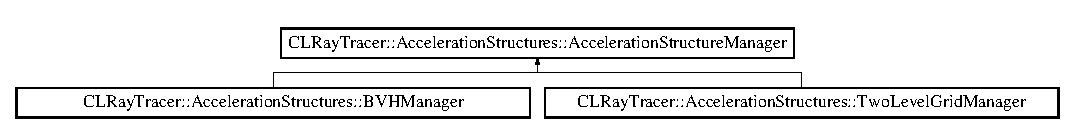
\includegraphics[height=1.355932cm]{class_c_l_ray_tracer_1_1_acceleration_structures_1_1_acceleration_structure_manager}
\end{center}
\end{figure}
\subsection*{Public Member Functions}
\begin{DoxyCompactItemize}
\item 
\hyperlink{class_c_l_ray_tracer_1_1_acceleration_structures_1_1_acceleration_structure_manager_a50ed7c8983555244b1c70728404156c0}{Acceleration\+Structure\+Manager} (const \hyperlink{class_c_l_ray_tracer_1_1_open_c_l_utils_1_1_c_l_execution_context}{Open\+C\+L\+Utils\+::\+C\+L\+Execution\+Context} \&context, const \hyperlink{class_c_l_ray_tracer_1_1_scene}{Scene} \&scene)
\item 
virtual \hyperlink{_errata_8h_a389396702f1aff6e71eb21328b0775c1}{Common\+::\+Result} \hyperlink{class_c_l_ray_tracer_1_1_acceleration_structures_1_1_acceleration_structure_manager_a14a5bacd261ea5c3e541ae531a128e4d}{initialize} (\hyperlink{class_c_l_ray_tracer_1_1_common_1_1_errata}{Common\+::\+Errata} \&err)=0
\item 
virtual \hyperlink{_errata_8h_a389396702f1aff6e71eb21328b0775c1}{Common\+::\+Result} \hyperlink{class_c_l_ray_tracer_1_1_acceleration_structures_1_1_acceleration_structure_manager_a3707d7588ce68855e6f086022025f1ea}{initialize\+Frame} (\hyperlink{class_c_l_ray_tracer_1_1_common_1_1_errata}{Common\+::\+Errata} \&err)=0
\item 
virtual \hyperlink{_errata_8h_a389396702f1aff6e71eb21328b0775c1}{Common\+::\+Result} \hyperlink{class_c_l_ray_tracer_1_1_acceleration_structures_1_1_acceleration_structure_manager_a29e770ee9fa4febf24f55ecf202d352b}{construct} (\hyperlink{class_c_l_ray_tracer_1_1_common_1_1_errata}{Common\+::\+Errata} \&err)=0
\item 
virtual \hyperlink{_errata_8h_a389396702f1aff6e71eb21328b0775c1}{Common\+::\+Result} \hyperlink{class_c_l_ray_tracer_1_1_acceleration_structures_1_1_acceleration_structure_manager_ab94dc605d1cee5c93de253bce69f21ca}{generate\+Contacts} (\hyperlink{struct_camera}{Camera} \&cam, \hyperlink{class_c_l_ray_tracer_1_1_common_1_1_errata}{Common\+::\+Errata} \&err)=0
\item 
virtual \hyperlink{_errata_8h_a389396702f1aff6e71eb21328b0775c1}{Common\+::\+Result} \hyperlink{class_c_l_ray_tracer_1_1_acceleration_structures_1_1_acceleration_structure_manager_aaa7b1d615a20126278ef27f0a5f3215c}{generate\+Contacts} (\hyperlink{class_c_l_ray_tracer_1_1_open_c_l_utils_1_1_c_l_buffer}{Open\+C\+L\+Utils\+::\+C\+L\+Buffer} \&rays, \hyperlink{class_c_l_ray_tracer_1_1_open_c_l_utils_1_1_c_l_buffer}{Open\+C\+L\+Utils\+::\+C\+L\+Buffer} \&contacts, const unsigned int ray\+Count, \hyperlink{class_c_l_ray_tracer_1_1_common_1_1_errata}{Common\+::\+Errata} \&err)=0
\item 
virtual const boost\+::shared\+\_\+ptr$<$ \hyperlink{class_c_l_ray_tracer_1_1_open_c_l_utils_1_1_c_l_buffer}{Open\+C\+L\+Utils\+::\+C\+L\+Buffer} $>$ \hyperlink{class_c_l_ray_tracer_1_1_acceleration_structures_1_1_acceleration_structure_manager_aeaaccc5dde154278325f1596b7bcde31}{get\+Primary\+Contacts} () const  =0
\item 
virtual \hyperlink{class_c_l_ray_tracer_1_1_acceleration_structures_1_1_acceleration_structure_manager_ae8cf037841560eab42f7e24825148dfa}{$\sim$\+Acceleration\+Structure\+Manager} ()
\end{DoxyCompactItemize}
\subsection*{Protected Attributes}
\begin{DoxyCompactItemize}
\item 
const \hyperlink{class_c_l_ray_tracer_1_1_open_c_l_utils_1_1_c_l_execution_context}{Open\+C\+L\+Utils\+::\+C\+L\+Execution\+Context} \& {\bfseries \+\_\+context}\hypertarget{class_c_l_ray_tracer_1_1_acceleration_structures_1_1_acceleration_structure_manager_a4c1c3733109f09d667356d2cf7ebfc02}{}\label{class_c_l_ray_tracer_1_1_acceleration_structures_1_1_acceleration_structure_manager_a4c1c3733109f09d667356d2cf7ebfc02}

\item 
const \hyperlink{class_c_l_ray_tracer_1_1_scene}{Scene} \& {\bfseries \+\_\+scene}\hypertarget{class_c_l_ray_tracer_1_1_acceleration_structures_1_1_acceleration_structure_manager_aed0c1306313fc485bd670ca76173af1c}{}\label{class_c_l_ray_tracer_1_1_acceleration_structures_1_1_acceleration_structure_manager_aed0c1306313fc485bd670ca76173af1c}

\end{DoxyCompactItemize}


\subsection{Detailed Description}
class \hyperlink{class_c_l_ray_tracer_1_1_acceleration_structures_1_1_acceleration_structure_manager}{Acceleration\+Structure\+Manager} -\/ The base class for acceleration structures for \hyperlink{struct_ray}{Ray} Tracing 

\subsection{Constructor \& Destructor Documentation}
\index{C\+L\+Ray\+Tracer\+::\+Acceleration\+Structures\+::\+Acceleration\+Structure\+Manager@{C\+L\+Ray\+Tracer\+::\+Acceleration\+Structures\+::\+Acceleration\+Structure\+Manager}!Acceleration\+Structure\+Manager@{Acceleration\+Structure\+Manager}}
\index{Acceleration\+Structure\+Manager@{Acceleration\+Structure\+Manager}!C\+L\+Ray\+Tracer\+::\+Acceleration\+Structures\+::\+Acceleration\+Structure\+Manager@{C\+L\+Ray\+Tracer\+::\+Acceleration\+Structures\+::\+Acceleration\+Structure\+Manager}}
\subsubsection[{\texorpdfstring{Acceleration\+Structure\+Manager(const Open\+C\+L\+Utils\+::\+C\+L\+Execution\+Context \&context, const Scene \&scene)}{AccelerationStructureManager(const OpenCLUtils::CLExecutionContext &context, const Scene &scene)}}]{\setlength{\rightskip}{0pt plus 5cm}C\+L\+Ray\+Tracer\+::\+Acceleration\+Structures\+::\+Acceleration\+Structure\+Manager\+::\+Acceleration\+Structure\+Manager (
\begin{DoxyParamCaption}
\item[{const {\bf Open\+C\+L\+Utils\+::\+C\+L\+Execution\+Context} \&}]{context, }
\item[{const {\bf Scene} \&}]{scene}
\end{DoxyParamCaption}
)\hspace{0.3cm}{\ttfamily [inline]}}\hypertarget{class_c_l_ray_tracer_1_1_acceleration_structures_1_1_acceleration_structure_manager_a50ed7c8983555244b1c70728404156c0}{}\label{class_c_l_ray_tracer_1_1_acceleration_structures_1_1_acceleration_structure_manager_a50ed7c8983555244b1c70728404156c0}
Constructor \index{C\+L\+Ray\+Tracer\+::\+Acceleration\+Structures\+::\+Acceleration\+Structure\+Manager@{C\+L\+Ray\+Tracer\+::\+Acceleration\+Structures\+::\+Acceleration\+Structure\+Manager}!````~Acceleration\+Structure\+Manager@{$\sim$\+Acceleration\+Structure\+Manager}}
\index{````~Acceleration\+Structure\+Manager@{$\sim$\+Acceleration\+Structure\+Manager}!C\+L\+Ray\+Tracer\+::\+Acceleration\+Structures\+::\+Acceleration\+Structure\+Manager@{C\+L\+Ray\+Tracer\+::\+Acceleration\+Structures\+::\+Acceleration\+Structure\+Manager}}
\subsubsection[{\texorpdfstring{$\sim$\+Acceleration\+Structure\+Manager()}{~AccelerationStructureManager()}}]{\setlength{\rightskip}{0pt plus 5cm}virtual C\+L\+Ray\+Tracer\+::\+Acceleration\+Structures\+::\+Acceleration\+Structure\+Manager\+::$\sim$\+Acceleration\+Structure\+Manager (
\begin{DoxyParamCaption}
{}
\end{DoxyParamCaption}
)\hspace{0.3cm}{\ttfamily [inline]}, {\ttfamily [virtual]}}\hypertarget{class_c_l_ray_tracer_1_1_acceleration_structures_1_1_acceleration_structure_manager_ae8cf037841560eab42f7e24825148dfa}{}\label{class_c_l_ray_tracer_1_1_acceleration_structures_1_1_acceleration_structure_manager_ae8cf037841560eab42f7e24825148dfa}
Destructor 

\subsection{Member Function Documentation}
\index{C\+L\+Ray\+Tracer\+::\+Acceleration\+Structures\+::\+Acceleration\+Structure\+Manager@{C\+L\+Ray\+Tracer\+::\+Acceleration\+Structures\+::\+Acceleration\+Structure\+Manager}!construct@{construct}}
\index{construct@{construct}!C\+L\+Ray\+Tracer\+::\+Acceleration\+Structures\+::\+Acceleration\+Structure\+Manager@{C\+L\+Ray\+Tracer\+::\+Acceleration\+Structures\+::\+Acceleration\+Structure\+Manager}}
\subsubsection[{\texorpdfstring{construct(\+Common\+::\+Errata \&err)=0}{construct(Common::Errata &err)=0}}]{\setlength{\rightskip}{0pt plus 5cm}virtual {\bf Common\+::\+Result} C\+L\+Ray\+Tracer\+::\+Acceleration\+Structures\+::\+Acceleration\+Structure\+Manager\+::construct (
\begin{DoxyParamCaption}
\item[{{\bf Common\+::\+Errata} \&}]{err}
\end{DoxyParamCaption}
)\hspace{0.3cm}{\ttfamily [pure virtual]}}\hypertarget{class_c_l_ray_tracer_1_1_acceleration_structures_1_1_acceleration_structure_manager_a29e770ee9fa4febf24f55ecf202d352b}{}\label{class_c_l_ray_tracer_1_1_acceleration_structures_1_1_acceleration_structure_manager_a29e770ee9fa4febf24f55ecf202d352b}
Constructs the acceleration structure according to the scene 

Implemented in \hyperlink{class_c_l_ray_tracer_1_1_acceleration_structures_1_1_two_level_grid_manager_a21edb29908807e8f2ba8c97d79758e05}{C\+L\+Ray\+Tracer\+::\+Acceleration\+Structures\+::\+Two\+Level\+Grid\+Manager}, and \hyperlink{class_c_l_ray_tracer_1_1_acceleration_structures_1_1_b_v_h_manager_a291018a731286a7f0d486b1cfc20bcdc}{C\+L\+Ray\+Tracer\+::\+Acceleration\+Structures\+::\+B\+V\+H\+Manager}.

\index{C\+L\+Ray\+Tracer\+::\+Acceleration\+Structures\+::\+Acceleration\+Structure\+Manager@{C\+L\+Ray\+Tracer\+::\+Acceleration\+Structures\+::\+Acceleration\+Structure\+Manager}!generate\+Contacts@{generate\+Contacts}}
\index{generate\+Contacts@{generate\+Contacts}!C\+L\+Ray\+Tracer\+::\+Acceleration\+Structures\+::\+Acceleration\+Structure\+Manager@{C\+L\+Ray\+Tracer\+::\+Acceleration\+Structures\+::\+Acceleration\+Structure\+Manager}}
\subsubsection[{\texorpdfstring{generate\+Contacts(\+Camera \&cam, Common\+::\+Errata \&err)=0}{generateContacts(Camera &cam, Common::Errata &err)=0}}]{\setlength{\rightskip}{0pt plus 5cm}virtual {\bf Common\+::\+Result} C\+L\+Ray\+Tracer\+::\+Acceleration\+Structures\+::\+Acceleration\+Structure\+Manager\+::generate\+Contacts (
\begin{DoxyParamCaption}
\item[{{\bf Camera} \&}]{cam, }
\item[{{\bf Common\+::\+Errata} \&}]{err}
\end{DoxyParamCaption}
)\hspace{0.3cm}{\ttfamily [pure virtual]}}\hypertarget{class_c_l_ray_tracer_1_1_acceleration_structures_1_1_acceleration_structure_manager_ab94dc605d1cee5c93de253bce69f21ca}{}\label{class_c_l_ray_tracer_1_1_acceleration_structures_1_1_acceleration_structure_manager_ab94dc605d1cee5c93de253bce69f21ca}
Generates contacts for viewing rays and fills the primary contacts array 

Implemented in \hyperlink{class_c_l_ray_tracer_1_1_acceleration_structures_1_1_two_level_grid_manager_a6a9f7a79568bfeb475a1ae9e1f88439d}{C\+L\+Ray\+Tracer\+::\+Acceleration\+Structures\+::\+Two\+Level\+Grid\+Manager}, and \hyperlink{class_c_l_ray_tracer_1_1_acceleration_structures_1_1_b_v_h_manager_acd5ef0664268cb587c5099b0994773a3}{C\+L\+Ray\+Tracer\+::\+Acceleration\+Structures\+::\+B\+V\+H\+Manager}.

\index{C\+L\+Ray\+Tracer\+::\+Acceleration\+Structures\+::\+Acceleration\+Structure\+Manager@{C\+L\+Ray\+Tracer\+::\+Acceleration\+Structures\+::\+Acceleration\+Structure\+Manager}!generate\+Contacts@{generate\+Contacts}}
\index{generate\+Contacts@{generate\+Contacts}!C\+L\+Ray\+Tracer\+::\+Acceleration\+Structures\+::\+Acceleration\+Structure\+Manager@{C\+L\+Ray\+Tracer\+::\+Acceleration\+Structures\+::\+Acceleration\+Structure\+Manager}}
\subsubsection[{\texorpdfstring{generate\+Contacts(\+Open\+C\+L\+Utils\+::\+C\+L\+Buffer \&rays, Open\+C\+L\+Utils\+::\+C\+L\+Buffer \&contacts, const unsigned int ray\+Count, Common\+::\+Errata \&err)=0}{generateContacts(OpenCLUtils::CLBuffer &rays, OpenCLUtils::CLBuffer &contacts, const unsigned int rayCount, Common::Errata &err)=0}}]{\setlength{\rightskip}{0pt plus 5cm}virtual {\bf Common\+::\+Result} C\+L\+Ray\+Tracer\+::\+Acceleration\+Structures\+::\+Acceleration\+Structure\+Manager\+::generate\+Contacts (
\begin{DoxyParamCaption}
\item[{{\bf Open\+C\+L\+Utils\+::\+C\+L\+Buffer} \&}]{rays, }
\item[{{\bf Open\+C\+L\+Utils\+::\+C\+L\+Buffer} \&}]{contacts, }
\item[{const unsigned int}]{ray\+Count, }
\item[{{\bf Common\+::\+Errata} \&}]{err}
\end{DoxyParamCaption}
)\hspace{0.3cm}{\ttfamily [pure virtual]}}\hypertarget{class_c_l_ray_tracer_1_1_acceleration_structures_1_1_acceleration_structure_manager_aaa7b1d615a20126278ef27f0a5f3215c}{}\label{class_c_l_ray_tracer_1_1_acceleration_structures_1_1_acceleration_structure_manager_aaa7b1d615a20126278ef27f0a5f3215c}
Generates contacts for rays and fills the contacts array 

Implemented in \hyperlink{class_c_l_ray_tracer_1_1_acceleration_structures_1_1_two_level_grid_manager_a186e22b86431d2b1c0fb92775bf6494b}{C\+L\+Ray\+Tracer\+::\+Acceleration\+Structures\+::\+Two\+Level\+Grid\+Manager}, and \hyperlink{class_c_l_ray_tracer_1_1_acceleration_structures_1_1_b_v_h_manager_a632bf0cb2fdf48ce3f04b16a4f64e615}{C\+L\+Ray\+Tracer\+::\+Acceleration\+Structures\+::\+B\+V\+H\+Manager}.

\index{C\+L\+Ray\+Tracer\+::\+Acceleration\+Structures\+::\+Acceleration\+Structure\+Manager@{C\+L\+Ray\+Tracer\+::\+Acceleration\+Structures\+::\+Acceleration\+Structure\+Manager}!get\+Primary\+Contacts@{get\+Primary\+Contacts}}
\index{get\+Primary\+Contacts@{get\+Primary\+Contacts}!C\+L\+Ray\+Tracer\+::\+Acceleration\+Structures\+::\+Acceleration\+Structure\+Manager@{C\+L\+Ray\+Tracer\+::\+Acceleration\+Structures\+::\+Acceleration\+Structure\+Manager}}
\subsubsection[{\texorpdfstring{get\+Primary\+Contacts() const  =0}{getPrimaryContacts() const  =0}}]{\setlength{\rightskip}{0pt plus 5cm}virtual const boost\+::shared\+\_\+ptr$<${\bf Open\+C\+L\+Utils\+::\+C\+L\+Buffer}$>$ C\+L\+Ray\+Tracer\+::\+Acceleration\+Structures\+::\+Acceleration\+Structure\+Manager\+::get\+Primary\+Contacts (
\begin{DoxyParamCaption}
{}
\end{DoxyParamCaption}
) const\hspace{0.3cm}{\ttfamily [pure virtual]}}\hypertarget{class_c_l_ray_tracer_1_1_acceleration_structures_1_1_acceleration_structure_manager_aeaaccc5dde154278325f1596b7bcde31}{}\label{class_c_l_ray_tracer_1_1_acceleration_structures_1_1_acceleration_structure_manager_aeaaccc5dde154278325f1596b7bcde31}
Retrieves the buffer of contacts that were the result of generate\+Contacts functions above 

Implemented in \hyperlink{class_c_l_ray_tracer_1_1_acceleration_structures_1_1_two_level_grid_manager_ac9a677d9c2085971cd4ba758ef4be43c}{C\+L\+Ray\+Tracer\+::\+Acceleration\+Structures\+::\+Two\+Level\+Grid\+Manager}, and \hyperlink{class_c_l_ray_tracer_1_1_acceleration_structures_1_1_b_v_h_manager_aedde0f4455f69e2b7854b1aae0e3583b}{C\+L\+Ray\+Tracer\+::\+Acceleration\+Structures\+::\+B\+V\+H\+Manager}.

\index{C\+L\+Ray\+Tracer\+::\+Acceleration\+Structures\+::\+Acceleration\+Structure\+Manager@{C\+L\+Ray\+Tracer\+::\+Acceleration\+Structures\+::\+Acceleration\+Structure\+Manager}!initialize@{initialize}}
\index{initialize@{initialize}!C\+L\+Ray\+Tracer\+::\+Acceleration\+Structures\+::\+Acceleration\+Structure\+Manager@{C\+L\+Ray\+Tracer\+::\+Acceleration\+Structures\+::\+Acceleration\+Structure\+Manager}}
\subsubsection[{\texorpdfstring{initialize(\+Common\+::\+Errata \&err)=0}{initialize(Common::Errata &err)=0}}]{\setlength{\rightskip}{0pt plus 5cm}virtual {\bf Common\+::\+Result} C\+L\+Ray\+Tracer\+::\+Acceleration\+Structures\+::\+Acceleration\+Structure\+Manager\+::initialize (
\begin{DoxyParamCaption}
\item[{{\bf Common\+::\+Errata} \&}]{err}
\end{DoxyParamCaption}
)\hspace{0.3cm}{\ttfamily [pure virtual]}}\hypertarget{class_c_l_ray_tracer_1_1_acceleration_structures_1_1_acceleration_structure_manager_a14a5bacd261ea5c3e541ae531a128e4d}{}\label{class_c_l_ray_tracer_1_1_acceleration_structures_1_1_acceleration_structure_manager_a14a5bacd261ea5c3e541ae531a128e4d}
General initialization of the acceleration structure managers -\/ Compiles kernels, etc 

Implemented in \hyperlink{class_c_l_ray_tracer_1_1_acceleration_structures_1_1_two_level_grid_manager_a98f2e5e78e14ebd09f23304b730d1696}{C\+L\+Ray\+Tracer\+::\+Acceleration\+Structures\+::\+Two\+Level\+Grid\+Manager}, and \hyperlink{class_c_l_ray_tracer_1_1_acceleration_structures_1_1_b_v_h_manager_aa84f753d471803ed8d7df36ecd384d3b}{C\+L\+Ray\+Tracer\+::\+Acceleration\+Structures\+::\+B\+V\+H\+Manager}.

\index{C\+L\+Ray\+Tracer\+::\+Acceleration\+Structures\+::\+Acceleration\+Structure\+Manager@{C\+L\+Ray\+Tracer\+::\+Acceleration\+Structures\+::\+Acceleration\+Structure\+Manager}!initialize\+Frame@{initialize\+Frame}}
\index{initialize\+Frame@{initialize\+Frame}!C\+L\+Ray\+Tracer\+::\+Acceleration\+Structures\+::\+Acceleration\+Structure\+Manager@{C\+L\+Ray\+Tracer\+::\+Acceleration\+Structures\+::\+Acceleration\+Structure\+Manager}}
\subsubsection[{\texorpdfstring{initialize\+Frame(\+Common\+::\+Errata \&err)=0}{initializeFrame(Common::Errata &err)=0}}]{\setlength{\rightskip}{0pt plus 5cm}virtual {\bf Common\+::\+Result} C\+L\+Ray\+Tracer\+::\+Acceleration\+Structures\+::\+Acceleration\+Structure\+Manager\+::initialize\+Frame (
\begin{DoxyParamCaption}
\item[{{\bf Common\+::\+Errata} \&}]{err}
\end{DoxyParamCaption}
)\hspace{0.3cm}{\ttfamily [pure virtual]}}\hypertarget{class_c_l_ray_tracer_1_1_acceleration_structures_1_1_acceleration_structure_manager_a3707d7588ce68855e6f086022025f1ea}{}\label{class_c_l_ray_tracer_1_1_acceleration_structures_1_1_acceleration_structure_manager_a3707d7588ce68855e6f086022025f1ea}
Prepares data for next frame -\/ Memory allocation, etc 

Implemented in \hyperlink{class_c_l_ray_tracer_1_1_acceleration_structures_1_1_two_level_grid_manager_a08dc7569f318a9422d69547331a31f16}{C\+L\+Ray\+Tracer\+::\+Acceleration\+Structures\+::\+Two\+Level\+Grid\+Manager}, and \hyperlink{class_c_l_ray_tracer_1_1_acceleration_structures_1_1_b_v_h_manager_a120b66507840a4e9b162ad4b3d863514}{C\+L\+Ray\+Tracer\+::\+Acceleration\+Structures\+::\+B\+V\+H\+Manager}.



The documentation for this class was generated from the following file\+:\begin{DoxyCompactItemize}
\item 
Include/\+Algorithms/\hyperlink{_acceleration_structure_manager_8h}{Acceleration\+Structure\+Manager.\+h}\end{DoxyCompactItemize}

\hypertarget{class_c_l_ray_tracer_1_1_common_1_1_bitonic_sort}{}\section{C\+L\+Ray\+Tracer\+:\+:Common\+:\+:Bitonic\+Sort Class Reference}
\label{class_c_l_ray_tracer_1_1_common_1_1_bitonic_sort}\index{C\+L\+Ray\+Tracer\+::\+Common\+::\+Bitonic\+Sort@{C\+L\+Ray\+Tracer\+::\+Common\+::\+Bitonic\+Sort}}


{\ttfamily \#include $<$Sorting.\+h$>$}

\subsection*{Public Member Functions}
\begin{DoxyCompactItemize}
\item 
\hyperlink{class_c_l_ray_tracer_1_1_common_1_1_bitonic_sort_afa3186a254bf1cc88bd5582f1ebc7f07}{Bitonic\+Sort} (const \hyperlink{class_c_l_ray_tracer_1_1_open_c_l_utils_1_1_c_l_execution_context}{Open\+C\+L\+Utils\+::\+C\+L\+Execution\+Context} \&context, const bool use\+Key\+Value)
\item 
\hyperlink{_errata_8h_a389396702f1aff6e71eb21328b0775c1}{Result} \hyperlink{class_c_l_ray_tracer_1_1_common_1_1_bitonic_sort_aa83725de0e4456f34f231efa8180adba}{initialize} (\hyperlink{class_c_l_ray_tracer_1_1_common_1_1_errata}{Errata} \&err)
\item 
\hyperlink{_errata_8h_a389396702f1aff6e71eb21328b0775c1}{Result} \hyperlink{class_c_l_ray_tracer_1_1_common_1_1_bitonic_sort_aef90e35777db561268d214d31104a160}{sort} (cl\+\_\+mem input, size\+\_\+t num\+\_\+items, \hyperlink{class_c_l_ray_tracer_1_1_common_1_1_errata}{Errata} \&err)
\end{DoxyCompactItemize}


\subsection{Detailed Description}
class \hyperlink{class_c_l_ray_tracer_1_1_common_1_1_bitonic_sort}{Bitonic\+Sort} Provides host interface for G\+PU implementation of Bitonic Sort 

\subsection{Constructor \& Destructor Documentation}
\index{C\+L\+Ray\+Tracer\+::\+Common\+::\+Bitonic\+Sort@{C\+L\+Ray\+Tracer\+::\+Common\+::\+Bitonic\+Sort}!Bitonic\+Sort@{Bitonic\+Sort}}
\index{Bitonic\+Sort@{Bitonic\+Sort}!C\+L\+Ray\+Tracer\+::\+Common\+::\+Bitonic\+Sort@{C\+L\+Ray\+Tracer\+::\+Common\+::\+Bitonic\+Sort}}
\subsubsection[{\texorpdfstring{Bitonic\+Sort(const Open\+C\+L\+Utils\+::\+C\+L\+Execution\+Context \&context, const bool use\+Key\+Value)}{BitonicSort(const OpenCLUtils::CLExecutionContext &context, const bool useKeyValue)}}]{\setlength{\rightskip}{0pt plus 5cm}C\+L\+Ray\+Tracer\+::\+Common\+::\+Bitonic\+Sort\+::\+Bitonic\+Sort (
\begin{DoxyParamCaption}
\item[{const {\bf Open\+C\+L\+Utils\+::\+C\+L\+Execution\+Context} \&}]{context, }
\item[{const bool}]{use\+Key\+Value}
\end{DoxyParamCaption}
)}\hypertarget{class_c_l_ray_tracer_1_1_common_1_1_bitonic_sort_afa3186a254bf1cc88bd5582f1ebc7f07}{}\label{class_c_l_ray_tracer_1_1_common_1_1_bitonic_sort_afa3186a254bf1cc88bd5582f1ebc7f07}
Constructor 
\begin{DoxyParams}{Parameters}
{\em context} & Open\+CL execution context \\
\hline
{\em use\+Key\+Value} & Indicates whether the sorted items are Key/\+Value pairs (C\+L\+\_\+\+U\+I\+N\+T2) or single values (C\+L\+\_\+\+U\+I\+NT) \\
\hline
\end{DoxyParams}


\subsection{Member Function Documentation}
\index{C\+L\+Ray\+Tracer\+::\+Common\+::\+Bitonic\+Sort@{C\+L\+Ray\+Tracer\+::\+Common\+::\+Bitonic\+Sort}!initialize@{initialize}}
\index{initialize@{initialize}!C\+L\+Ray\+Tracer\+::\+Common\+::\+Bitonic\+Sort@{C\+L\+Ray\+Tracer\+::\+Common\+::\+Bitonic\+Sort}}
\subsubsection[{\texorpdfstring{initialize(\+Errata \&err)}{initialize(Errata &err)}}]{\setlength{\rightskip}{0pt plus 5cm}{\bf Result} C\+L\+Ray\+Tracer\+::\+Common\+::\+Bitonic\+Sort\+::initialize (
\begin{DoxyParamCaption}
\item[{{\bf Errata} \&}]{err}
\end{DoxyParamCaption}
)}\hypertarget{class_c_l_ray_tracer_1_1_common_1_1_bitonic_sort_aa83725de0e4456f34f231efa8180adba}{}\label{class_c_l_ray_tracer_1_1_common_1_1_bitonic_sort_aa83725de0e4456f34f231efa8180adba}
Initialize Performs initialization of a \hyperlink{class_c_l_ray_tracer_1_1_common_1_1_bitonic_sort}{Bitonic\+Sort} instance. Must be called once per instance 
\begin{DoxyParams}[1]{Parameters}
\mbox{\tt out}  & {\em err} & Error info, in case error occurred \\
\hline
\end{DoxyParams}
\begin{DoxyReturn}{Returns}
Result, that indicates whether the operation succeeded or failed 
\end{DoxyReturn}
\index{C\+L\+Ray\+Tracer\+::\+Common\+::\+Bitonic\+Sort@{C\+L\+Ray\+Tracer\+::\+Common\+::\+Bitonic\+Sort}!sort@{sort}}
\index{sort@{sort}!C\+L\+Ray\+Tracer\+::\+Common\+::\+Bitonic\+Sort@{C\+L\+Ray\+Tracer\+::\+Common\+::\+Bitonic\+Sort}}
\subsubsection[{\texorpdfstring{sort(cl\+\_\+mem input, size\+\_\+t num\+\_\+items, Errata \&err)}{sort(cl_mem input, size_t num_items, Errata &err)}}]{\setlength{\rightskip}{0pt plus 5cm}{\bf Result} C\+L\+Ray\+Tracer\+::\+Common\+::\+Bitonic\+Sort\+::sort (
\begin{DoxyParamCaption}
\item[{cl\+\_\+mem}]{input, }
\item[{size\+\_\+t}]{num\+\_\+items, }
\item[{{\bf Errata} \&}]{err}
\end{DoxyParamCaption}
)}\hypertarget{class_c_l_ray_tracer_1_1_common_1_1_bitonic_sort_aef90e35777db561268d214d31104a160}{}\label{class_c_l_ray_tracer_1_1_common_1_1_bitonic_sort_aef90e35777db561268d214d31104a160}
Sorts the input array 
\begin{DoxyParams}[1]{Parameters}
 & {\em input} & Device pointer to array that shoud be sorted \\
\hline
 & {\em num\+\_\+items} & Number of items in array to be sorted -\/ Must be power of two \\
\hline
\mbox{\tt out}  & {\em err} & Error info, in case error occurred \\
\hline
\end{DoxyParams}
\begin{DoxyReturn}{Returns}
Result, that indicates whether the operation succeeded or failed 
\end{DoxyReturn}


The documentation for this class was generated from the following file\+:\begin{DoxyCompactItemize}
\item 
Include/\+Algorithms/\hyperlink{_sorting_8h}{Sorting.\+h}\end{DoxyCompactItemize}

\hypertarget{class_c_l_ray_tracer_1_1_acceleration_structures_1_1_b_v_h_manager}{}\section{C\+L\+Ray\+Tracer\+:\+:Acceleration\+Structures\+:\+:B\+V\+H\+Manager Class Reference}
\label{class_c_l_ray_tracer_1_1_acceleration_structures_1_1_b_v_h_manager}\index{C\+L\+Ray\+Tracer\+::\+Acceleration\+Structures\+::\+B\+V\+H\+Manager@{C\+L\+Ray\+Tracer\+::\+Acceleration\+Structures\+::\+B\+V\+H\+Manager}}


{\ttfamily \#include $<$B\+V\+H\+Manager.\+h$>$}

Inheritance diagram for C\+L\+Ray\+Tracer\+:\+:Acceleration\+Structures\+:\+:B\+V\+H\+Manager\+:\begin{figure}[H]
\begin{center}
\leavevmode
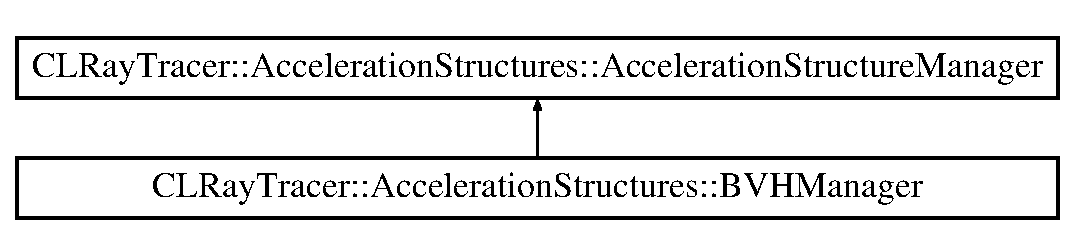
\includegraphics[height=2.000000cm]{class_c_l_ray_tracer_1_1_acceleration_structures_1_1_b_v_h_manager}
\end{center}
\end{figure}
\subsection*{Public Member Functions}
\begin{DoxyCompactItemize}
\item 
\hyperlink{class_c_l_ray_tracer_1_1_acceleration_structures_1_1_b_v_h_manager_a44c7d81fb8a8fbf07208219261233bf5}{B\+V\+H\+Manager} (const \hyperlink{class_c_l_ray_tracer_1_1_open_c_l_utils_1_1_c_l_execution_context}{Open\+C\+L\+Utils\+::\+C\+L\+Execution\+Context} \&context, const \hyperlink{class_c_l_ray_tracer_1_1_scene}{Scene} \&scene)
\item 
virtual \hyperlink{_errata_8h_a389396702f1aff6e71eb21328b0775c1}{Common\+::\+Result} \hyperlink{class_c_l_ray_tracer_1_1_acceleration_structures_1_1_b_v_h_manager_aa84f753d471803ed8d7df36ecd384d3b}{initialize} (\hyperlink{class_c_l_ray_tracer_1_1_common_1_1_errata}{Common\+::\+Errata} \&err)
\item 
virtual \hyperlink{_errata_8h_a389396702f1aff6e71eb21328b0775c1}{Common\+::\+Result} \hyperlink{class_c_l_ray_tracer_1_1_acceleration_structures_1_1_b_v_h_manager_a120b66507840a4e9b162ad4b3d863514}{initialize\+Frame} (\hyperlink{class_c_l_ray_tracer_1_1_common_1_1_errata}{Common\+::\+Errata} \&err)
\item 
virtual \hyperlink{_errata_8h_a389396702f1aff6e71eb21328b0775c1}{Common\+::\+Result} \hyperlink{class_c_l_ray_tracer_1_1_acceleration_structures_1_1_b_v_h_manager_a291018a731286a7f0d486b1cfc20bcdc}{construct} (\hyperlink{class_c_l_ray_tracer_1_1_common_1_1_errata}{Common\+::\+Errata} \&err)
\item 
virtual \hyperlink{_errata_8h_a389396702f1aff6e71eb21328b0775c1}{Common\+::\+Result} \hyperlink{class_c_l_ray_tracer_1_1_acceleration_structures_1_1_b_v_h_manager_acd5ef0664268cb587c5099b0994773a3}{generate\+Contacts} (\hyperlink{struct_camera}{Camera} \&cam, \hyperlink{class_c_l_ray_tracer_1_1_common_1_1_errata}{Common\+::\+Errata} \&err)
\item 
virtual \hyperlink{_errata_8h_a389396702f1aff6e71eb21328b0775c1}{Common\+::\+Result} \hyperlink{class_c_l_ray_tracer_1_1_acceleration_structures_1_1_b_v_h_manager_a632bf0cb2fdf48ce3f04b16a4f64e615}{generate\+Contacts} (\hyperlink{class_c_l_ray_tracer_1_1_open_c_l_utils_1_1_c_l_buffer}{Open\+C\+L\+Utils\+::\+C\+L\+Buffer} \&rays, \hyperlink{class_c_l_ray_tracer_1_1_open_c_l_utils_1_1_c_l_buffer}{Open\+C\+L\+Utils\+::\+C\+L\+Buffer} \&contacts, const unsigned int ray\+Count, \hyperlink{class_c_l_ray_tracer_1_1_common_1_1_errata}{Common\+::\+Errata} \&err)
\item 
virtual const boost\+::shared\+\_\+ptr$<$ \hyperlink{class_c_l_ray_tracer_1_1_open_c_l_utils_1_1_c_l_buffer}{Open\+C\+L\+Utils\+::\+C\+L\+Buffer} $>$ \hyperlink{class_c_l_ray_tracer_1_1_acceleration_structures_1_1_b_v_h_manager_aedde0f4455f69e2b7854b1aae0e3583b}{get\+Primary\+Contacts} () const 
\end{DoxyCompactItemize}
\subsection*{Protected Attributes}
\begin{DoxyCompactItemize}
\item 
C\+L\+\_\+\+U\+I\+NT {\bfseries \+\_\+morton\+Buffer\+Items}\hypertarget{class_c_l_ray_tracer_1_1_acceleration_structures_1_1_b_v_h_manager_a0860ba563afc7145e63b96657372f448}{}\label{class_c_l_ray_tracer_1_1_acceleration_structures_1_1_b_v_h_manager_a0860ba563afc7145e63b96657372f448}

\item 
C\+L\+\_\+\+U\+L\+O\+NG {\bfseries \+\_\+device\+Local\+Memory}\hypertarget{class_c_l_ray_tracer_1_1_acceleration_structures_1_1_b_v_h_manager_aafff3e0424c27db3cad4e90153459a1b}{}\label{class_c_l_ray_tracer_1_1_acceleration_structures_1_1_b_v_h_manager_aafff3e0424c27db3cad4e90153459a1b}

\item 
C\+L\+\_\+\+U\+I\+NT {\bfseries \+\_\+bvh\+Leaves\+Count}\hypertarget{class_c_l_ray_tracer_1_1_acceleration_structures_1_1_b_v_h_manager_a26cbdacbf7d0be22160438df6dcf5616}{}\label{class_c_l_ray_tracer_1_1_acceleration_structures_1_1_b_v_h_manager_a26cbdacbf7d0be22160438df6dcf5616}

\item 
boost\+::shared\+\_\+ptr$<$ \hyperlink{class_c_l_ray_tracer_1_1_common_1_1_bitonic_sort}{Common\+::\+Bitonic\+Sort} $>$ {\bfseries \+\_\+bitonic\+Sorter}\hypertarget{class_c_l_ray_tracer_1_1_acceleration_structures_1_1_b_v_h_manager_a687c33b2d71e8b5e5bcbface128b5719}{}\label{class_c_l_ray_tracer_1_1_acceleration_structures_1_1_b_v_h_manager_a687c33b2d71e8b5e5bcbface128b5719}

\item 
boost\+::shared\+\_\+ptr$<$ \hyperlink{class_c_l_ray_tracer_1_1_open_c_l_utils_1_1_c_l_buffer}{Open\+C\+L\+Utils\+::\+C\+L\+Buffer} $>$ {\bfseries \+\_\+bvh\+Nodes}\hypertarget{class_c_l_ray_tracer_1_1_acceleration_structures_1_1_b_v_h_manager_a9ea330778738a1e467c234e5c04edd9d}{}\label{class_c_l_ray_tracer_1_1_acceleration_structures_1_1_b_v_h_manager_a9ea330778738a1e467c234e5c04edd9d}

\item 
boost\+::shared\+\_\+ptr$<$ \hyperlink{class_c_l_ray_tracer_1_1_open_c_l_utils_1_1_c_l_buffer}{Open\+C\+L\+Utils\+::\+C\+L\+Buffer} $>$ {\bfseries \+\_\+sorted\+Morton\+Codes}\hypertarget{class_c_l_ray_tracer_1_1_acceleration_structures_1_1_b_v_h_manager_aa1dbd2e89b8079f7ba8c82030f1f338d}{}\label{class_c_l_ray_tracer_1_1_acceleration_structures_1_1_b_v_h_manager_aa1dbd2e89b8079f7ba8c82030f1f338d}

\item 
boost\+::shared\+\_\+ptr$<$ \hyperlink{class_c_l_ray_tracer_1_1_open_c_l_utils_1_1_c_l_buffer}{Open\+C\+L\+Utils\+::\+C\+L\+Buffer} $>$ {\bfseries \+\_\+node\+Visit\+Counters}\hypertarget{class_c_l_ray_tracer_1_1_acceleration_structures_1_1_b_v_h_manager_ace735a73db08ade00aca02fc4f85de83}{}\label{class_c_l_ray_tracer_1_1_acceleration_structures_1_1_b_v_h_manager_ace735a73db08ade00aca02fc4f85de83}

\item 
boost\+::shared\+\_\+ptr$<$ \hyperlink{class_c_l_ray_tracer_1_1_open_c_l_utils_1_1_c_l_buffer}{Open\+C\+L\+Utils\+::\+C\+L\+Buffer} $>$ {\bfseries \+\_\+primary\+Contacts\+Array}\hypertarget{class_c_l_ray_tracer_1_1_acceleration_structures_1_1_b_v_h_manager_aaee13b21f30e03f10cd686a8522fdbf9}{}\label{class_c_l_ray_tracer_1_1_acceleration_structures_1_1_b_v_h_manager_aaee13b21f30e03f10cd686a8522fdbf9}

\item 
boost\+::shared\+\_\+ptr$<$ \hyperlink{class_c_l_ray_tracer_1_1_open_c_l_utils_1_1_c_l_buffer}{Open\+C\+L\+Utils\+::\+C\+L\+Buffer} $>$ {\bfseries \+\_\+device\+Camera}\hypertarget{class_c_l_ray_tracer_1_1_acceleration_structures_1_1_b_v_h_manager_ab04c1e2bdc5f2431ebf11730ab175570}{}\label{class_c_l_ray_tracer_1_1_acceleration_structures_1_1_b_v_h_manager_ab04c1e2bdc5f2431ebf11730ab175570}

\item 
boost\+::shared\+\_\+ptr$<$ \hyperlink{class_c_l_ray_tracer_1_1_open_c_l_utils_1_1_c_l_program}{Open\+C\+L\+Utils\+::\+C\+L\+Program} $>$ {\bfseries \+\_\+bvh\+Program}\hypertarget{class_c_l_ray_tracer_1_1_acceleration_structures_1_1_b_v_h_manager_a5b3813130c50e428c4e3d482e2c78736}{}\label{class_c_l_ray_tracer_1_1_acceleration_structures_1_1_b_v_h_manager_a5b3813130c50e428c4e3d482e2c78736}

\item 
boost\+::shared\+\_\+ptr$<$ \hyperlink{class_c_l_ray_tracer_1_1_open_c_l_utils_1_1_c_l_kernel}{Open\+C\+L\+Utils\+::\+C\+L\+Kernel} $>$ {\bfseries \+\_\+morton\+Calc\+Kernel}\hypertarget{class_c_l_ray_tracer_1_1_acceleration_structures_1_1_b_v_h_manager_a45d2f052bcd80fd4a8f0c3d56fe0e96d}{}\label{class_c_l_ray_tracer_1_1_acceleration_structures_1_1_b_v_h_manager_a45d2f052bcd80fd4a8f0c3d56fe0e96d}

\item 
boost\+::shared\+\_\+ptr$<$ \hyperlink{class_c_l_ray_tracer_1_1_open_c_l_utils_1_1_c_l_kernel}{Open\+C\+L\+Utils\+::\+C\+L\+Kernel} $>$ {\bfseries \+\_\+radix\+Tree\+Build\+Kernel}\hypertarget{class_c_l_ray_tracer_1_1_acceleration_structures_1_1_b_v_h_manager_ad10eceea8e568086444e8a805c971ff8}{}\label{class_c_l_ray_tracer_1_1_acceleration_structures_1_1_b_v_h_manager_ad10eceea8e568086444e8a805c971ff8}

\item 
boost\+::shared\+\_\+ptr$<$ \hyperlink{class_c_l_ray_tracer_1_1_open_c_l_utils_1_1_c_l_kernel}{Open\+C\+L\+Utils\+::\+C\+L\+Kernel} $>$ {\bfseries \+\_\+bb\+Calc\+Kernel}\hypertarget{class_c_l_ray_tracer_1_1_acceleration_structures_1_1_b_v_h_manager_a0f8da82584c796cda7c3d29cca9df485}{}\label{class_c_l_ray_tracer_1_1_acceleration_structures_1_1_b_v_h_manager_a0f8da82584c796cda7c3d29cca9df485}

\item 
boost\+::shared\+\_\+ptr$<$ \hyperlink{class_c_l_ray_tracer_1_1_open_c_l_utils_1_1_c_l_kernel}{Open\+C\+L\+Utils\+::\+C\+L\+Kernel} $>$ {\bfseries \+\_\+contact\+Generate\+Kernel}\hypertarget{class_c_l_ray_tracer_1_1_acceleration_structures_1_1_b_v_h_manager_a0171f2a54bc88e68feb34d0a09548462}{}\label{class_c_l_ray_tracer_1_1_acceleration_structures_1_1_b_v_h_manager_a0171f2a54bc88e68feb34d0a09548462}

\item 
boost\+::shared\+\_\+ptr$<$ \hyperlink{class_c_l_ray_tracer_1_1_open_c_l_utils_1_1_c_l_kernel}{Open\+C\+L\+Utils\+::\+C\+L\+Kernel} $>$ {\bfseries \+\_\+contact\+Generate\+Kernel2}\hypertarget{class_c_l_ray_tracer_1_1_acceleration_structures_1_1_b_v_h_manager_aac462ea62721df4ac8266cc5ca24353d}{}\label{class_c_l_ray_tracer_1_1_acceleration_structures_1_1_b_v_h_manager_aac462ea62721df4ac8266cc5ca24353d}

\end{DoxyCompactItemize}


\subsection{Detailed Description}
class \hyperlink{class_c_l_ray_tracer_1_1_acceleration_structures_1_1_b_v_h_manager}{B\+V\+H\+Manager} -\/ The host interface to G\+PU implementation of B\+VH 

\subsection{Constructor \& Destructor Documentation}
\index{C\+L\+Ray\+Tracer\+::\+Acceleration\+Structures\+::\+B\+V\+H\+Manager@{C\+L\+Ray\+Tracer\+::\+Acceleration\+Structures\+::\+B\+V\+H\+Manager}!B\+V\+H\+Manager@{B\+V\+H\+Manager}}
\index{B\+V\+H\+Manager@{B\+V\+H\+Manager}!C\+L\+Ray\+Tracer\+::\+Acceleration\+Structures\+::\+B\+V\+H\+Manager@{C\+L\+Ray\+Tracer\+::\+Acceleration\+Structures\+::\+B\+V\+H\+Manager}}
\subsubsection[{\texorpdfstring{B\+V\+H\+Manager(const Open\+C\+L\+Utils\+::\+C\+L\+Execution\+Context \&context, const Scene \&scene)}{BVHManager(const OpenCLUtils::CLExecutionContext &context, const Scene &scene)}}]{\setlength{\rightskip}{0pt plus 5cm}C\+L\+Ray\+Tracer\+::\+Acceleration\+Structures\+::\+B\+V\+H\+Manager\+::\+B\+V\+H\+Manager (
\begin{DoxyParamCaption}
\item[{const {\bf Open\+C\+L\+Utils\+::\+C\+L\+Execution\+Context} \&}]{context, }
\item[{const {\bf Scene} \&}]{scene}
\end{DoxyParamCaption}
)}\hypertarget{class_c_l_ray_tracer_1_1_acceleration_structures_1_1_b_v_h_manager_a44c7d81fb8a8fbf07208219261233bf5}{}\label{class_c_l_ray_tracer_1_1_acceleration_structures_1_1_b_v_h_manager_a44c7d81fb8a8fbf07208219261233bf5}
Constructor 

\subsection{Member Function Documentation}
\index{C\+L\+Ray\+Tracer\+::\+Acceleration\+Structures\+::\+B\+V\+H\+Manager@{C\+L\+Ray\+Tracer\+::\+Acceleration\+Structures\+::\+B\+V\+H\+Manager}!construct@{construct}}
\index{construct@{construct}!C\+L\+Ray\+Tracer\+::\+Acceleration\+Structures\+::\+B\+V\+H\+Manager@{C\+L\+Ray\+Tracer\+::\+Acceleration\+Structures\+::\+B\+V\+H\+Manager}}
\subsubsection[{\texorpdfstring{construct(\+Common\+::\+Errata \&err)}{construct(Common::Errata &err)}}]{\setlength{\rightskip}{0pt plus 5cm}virtual {\bf Common\+::\+Result} C\+L\+Ray\+Tracer\+::\+Acceleration\+Structures\+::\+B\+V\+H\+Manager\+::construct (
\begin{DoxyParamCaption}
\item[{{\bf Common\+::\+Errata} \&}]{err}
\end{DoxyParamCaption}
)\hspace{0.3cm}{\ttfamily [virtual]}}\hypertarget{class_c_l_ray_tracer_1_1_acceleration_structures_1_1_b_v_h_manager_a291018a731286a7f0d486b1cfc20bcdc}{}\label{class_c_l_ray_tracer_1_1_acceleration_structures_1_1_b_v_h_manager_a291018a731286a7f0d486b1cfc20bcdc}
Constructs B\+VH acceleration structure, according to associated scene state 
\begin{DoxyParams}{Parameters}
{\em err} & Error info \\
\hline
\end{DoxyParams}
\begin{DoxyReturn}{Returns}
Result of the operation\+: Success or failure 
\end{DoxyReturn}


Implements \hyperlink{class_c_l_ray_tracer_1_1_acceleration_structures_1_1_acceleration_structure_manager_a29e770ee9fa4febf24f55ecf202d352b}{C\+L\+Ray\+Tracer\+::\+Acceleration\+Structures\+::\+Acceleration\+Structure\+Manager}.

\index{C\+L\+Ray\+Tracer\+::\+Acceleration\+Structures\+::\+B\+V\+H\+Manager@{C\+L\+Ray\+Tracer\+::\+Acceleration\+Structures\+::\+B\+V\+H\+Manager}!generate\+Contacts@{generate\+Contacts}}
\index{generate\+Contacts@{generate\+Contacts}!C\+L\+Ray\+Tracer\+::\+Acceleration\+Structures\+::\+B\+V\+H\+Manager@{C\+L\+Ray\+Tracer\+::\+Acceleration\+Structures\+::\+B\+V\+H\+Manager}}
\subsubsection[{\texorpdfstring{generate\+Contacts(\+Camera \&cam, Common\+::\+Errata \&err)}{generateContacts(Camera &cam, Common::Errata &err)}}]{\setlength{\rightskip}{0pt plus 5cm}virtual {\bf Common\+::\+Result} C\+L\+Ray\+Tracer\+::\+Acceleration\+Structures\+::\+B\+V\+H\+Manager\+::generate\+Contacts (
\begin{DoxyParamCaption}
\item[{{\bf Camera} \&}]{cam, }
\item[{{\bf Common\+::\+Errata} \&}]{err}
\end{DoxyParamCaption}
)\hspace{0.3cm}{\ttfamily [virtual]}}\hypertarget{class_c_l_ray_tracer_1_1_acceleration_structures_1_1_b_v_h_manager_acd5ef0664268cb587c5099b0994773a3}{}\label{class_c_l_ray_tracer_1_1_acceleration_structures_1_1_b_v_h_manager_acd5ef0664268cb587c5099b0994773a3}
Generates hit data for viewing rays, from the constructed B\+VH 
\begin{DoxyParams}{Parameters}
{\em err} & Error info \\
\hline
\end{DoxyParams}
\begin{DoxyReturn}{Returns}
Result of the operation\+: Success or failure 
\end{DoxyReturn}


Implements \hyperlink{class_c_l_ray_tracer_1_1_acceleration_structures_1_1_acceleration_structure_manager_ab94dc605d1cee5c93de253bce69f21ca}{C\+L\+Ray\+Tracer\+::\+Acceleration\+Structures\+::\+Acceleration\+Structure\+Manager}.

\index{C\+L\+Ray\+Tracer\+::\+Acceleration\+Structures\+::\+B\+V\+H\+Manager@{C\+L\+Ray\+Tracer\+::\+Acceleration\+Structures\+::\+B\+V\+H\+Manager}!generate\+Contacts@{generate\+Contacts}}
\index{generate\+Contacts@{generate\+Contacts}!C\+L\+Ray\+Tracer\+::\+Acceleration\+Structures\+::\+B\+V\+H\+Manager@{C\+L\+Ray\+Tracer\+::\+Acceleration\+Structures\+::\+B\+V\+H\+Manager}}
\subsubsection[{\texorpdfstring{generate\+Contacts(\+Open\+C\+L\+Utils\+::\+C\+L\+Buffer \&rays, Open\+C\+L\+Utils\+::\+C\+L\+Buffer \&contacts, const unsigned int ray\+Count, Common\+::\+Errata \&err)}{generateContacts(OpenCLUtils::CLBuffer &rays, OpenCLUtils::CLBuffer &contacts, const unsigned int rayCount, Common::Errata &err)}}]{\setlength{\rightskip}{0pt plus 5cm}virtual {\bf Common\+::\+Result} C\+L\+Ray\+Tracer\+::\+Acceleration\+Structures\+::\+B\+V\+H\+Manager\+::generate\+Contacts (
\begin{DoxyParamCaption}
\item[{{\bf Open\+C\+L\+Utils\+::\+C\+L\+Buffer} \&}]{rays, }
\item[{{\bf Open\+C\+L\+Utils\+::\+C\+L\+Buffer} \&}]{contacts, }
\item[{const unsigned int}]{ray\+Count, }
\item[{{\bf Common\+::\+Errata} \&}]{err}
\end{DoxyParamCaption}
)\hspace{0.3cm}{\ttfamily [virtual]}}\hypertarget{class_c_l_ray_tracer_1_1_acceleration_structures_1_1_b_v_h_manager_a632bf0cb2fdf48ce3f04b16a4f64e615}{}\label{class_c_l_ray_tracer_1_1_acceleration_structures_1_1_b_v_h_manager_a632bf0cb2fdf48ce3f04b16a4f64e615}
Generates contacts for rays and fills the contacts array 
\begin{DoxyParams}{Parameters}
{\em rays} & The rays to be traced -\/ A device memory buffer object that contains rays as struct \hyperlink{struct_ray}{Ray} \\
\hline
{\em contact} & The target device memory that will contain the result -\/ For each ray rays\mbox{[}i\mbox{]} the buffer will contain data about its closest intersection with object in the scene as contacts\mbox{[}i\mbox{]}. The contact data will be stored as struct \hyperlink{struct_contact}{Contact} \\
\hline
{\em ray\+Count} & The number of rays to trace \\
\hline
{\em err} & Error info \\
\hline
\end{DoxyParams}
\begin{DoxyReturn}{Returns}
Result of the operation\+: Success or failure 
\end{DoxyReturn}


Implements \hyperlink{class_c_l_ray_tracer_1_1_acceleration_structures_1_1_acceleration_structure_manager_aaa7b1d615a20126278ef27f0a5f3215c}{C\+L\+Ray\+Tracer\+::\+Acceleration\+Structures\+::\+Acceleration\+Structure\+Manager}.

\index{C\+L\+Ray\+Tracer\+::\+Acceleration\+Structures\+::\+B\+V\+H\+Manager@{C\+L\+Ray\+Tracer\+::\+Acceleration\+Structures\+::\+B\+V\+H\+Manager}!get\+Primary\+Contacts@{get\+Primary\+Contacts}}
\index{get\+Primary\+Contacts@{get\+Primary\+Contacts}!C\+L\+Ray\+Tracer\+::\+Acceleration\+Structures\+::\+B\+V\+H\+Manager@{C\+L\+Ray\+Tracer\+::\+Acceleration\+Structures\+::\+B\+V\+H\+Manager}}
\subsubsection[{\texorpdfstring{get\+Primary\+Contacts() const }{getPrimaryContacts() const }}]{\setlength{\rightskip}{0pt plus 5cm}virtual const boost\+::shared\+\_\+ptr$<${\bf Open\+C\+L\+Utils\+::\+C\+L\+Buffer}$>$ C\+L\+Ray\+Tracer\+::\+Acceleration\+Structures\+::\+B\+V\+H\+Manager\+::get\+Primary\+Contacts (
\begin{DoxyParamCaption}
{}
\end{DoxyParamCaption}
) const\hspace{0.3cm}{\ttfamily [inline]}, {\ttfamily [virtual]}}\hypertarget{class_c_l_ray_tracer_1_1_acceleration_structures_1_1_b_v_h_manager_aedde0f4455f69e2b7854b1aae0e3583b}{}\label{class_c_l_ray_tracer_1_1_acceleration_structures_1_1_b_v_h_manager_aedde0f4455f69e2b7854b1aae0e3583b}
Retrieves the buffer of contacts that were the result of generate\+Contacts functions above 

Implements \hyperlink{class_c_l_ray_tracer_1_1_acceleration_structures_1_1_acceleration_structure_manager_aeaaccc5dde154278325f1596b7bcde31}{C\+L\+Ray\+Tracer\+::\+Acceleration\+Structures\+::\+Acceleration\+Structure\+Manager}.

\index{C\+L\+Ray\+Tracer\+::\+Acceleration\+Structures\+::\+B\+V\+H\+Manager@{C\+L\+Ray\+Tracer\+::\+Acceleration\+Structures\+::\+B\+V\+H\+Manager}!initialize@{initialize}}
\index{initialize@{initialize}!C\+L\+Ray\+Tracer\+::\+Acceleration\+Structures\+::\+B\+V\+H\+Manager@{C\+L\+Ray\+Tracer\+::\+Acceleration\+Structures\+::\+B\+V\+H\+Manager}}
\subsubsection[{\texorpdfstring{initialize(\+Common\+::\+Errata \&err)}{initialize(Common::Errata &err)}}]{\setlength{\rightskip}{0pt plus 5cm}virtual {\bf Common\+::\+Result} C\+L\+Ray\+Tracer\+::\+Acceleration\+Structures\+::\+B\+V\+H\+Manager\+::initialize (
\begin{DoxyParamCaption}
\item[{{\bf Common\+::\+Errata} \&}]{err}
\end{DoxyParamCaption}
)\hspace{0.3cm}{\ttfamily [virtual]}}\hypertarget{class_c_l_ray_tracer_1_1_acceleration_structures_1_1_b_v_h_manager_aa84f753d471803ed8d7df36ecd384d3b}{}\label{class_c_l_ray_tracer_1_1_acceleration_structures_1_1_b_v_h_manager_aa84f753d471803ed8d7df36ecd384d3b}
Performs main initialization of the B\+VH structure. This initialization shoud be performed just once per instance. 
\begin{DoxyParams}{Parameters}
{\em err} & Error info \\
\hline
\end{DoxyParams}
\begin{DoxyReturn}{Returns}
Result of the operation\+: Success or failure 
\end{DoxyReturn}


Implements \hyperlink{class_c_l_ray_tracer_1_1_acceleration_structures_1_1_acceleration_structure_manager_a14a5bacd261ea5c3e541ae531a128e4d}{C\+L\+Ray\+Tracer\+::\+Acceleration\+Structures\+::\+Acceleration\+Structure\+Manager}.

\index{C\+L\+Ray\+Tracer\+::\+Acceleration\+Structures\+::\+B\+V\+H\+Manager@{C\+L\+Ray\+Tracer\+::\+Acceleration\+Structures\+::\+B\+V\+H\+Manager}!initialize\+Frame@{initialize\+Frame}}
\index{initialize\+Frame@{initialize\+Frame}!C\+L\+Ray\+Tracer\+::\+Acceleration\+Structures\+::\+B\+V\+H\+Manager@{C\+L\+Ray\+Tracer\+::\+Acceleration\+Structures\+::\+B\+V\+H\+Manager}}
\subsubsection[{\texorpdfstring{initialize\+Frame(\+Common\+::\+Errata \&err)}{initializeFrame(Common::Errata &err)}}]{\setlength{\rightskip}{0pt plus 5cm}virtual {\bf Common\+::\+Result} C\+L\+Ray\+Tracer\+::\+Acceleration\+Structures\+::\+B\+V\+H\+Manager\+::initialize\+Frame (
\begin{DoxyParamCaption}
\item[{{\bf Common\+::\+Errata} \&}]{err}
\end{DoxyParamCaption}
)\hspace{0.3cm}{\ttfamily [virtual]}}\hypertarget{class_c_l_ray_tracer_1_1_acceleration_structures_1_1_b_v_h_manager_a120b66507840a4e9b162ad4b3d863514}{}\label{class_c_l_ray_tracer_1_1_acceleration_structures_1_1_b_v_h_manager_a120b66507840a4e9b162ad4b3d863514}
Performs initialization of a frame for B\+VH acceleration structure This initialization shoud be performed before each frame. 
\begin{DoxyParams}{Parameters}
{\em err} & Error info \\
\hline
\end{DoxyParams}
\begin{DoxyReturn}{Returns}
Result of the operation\+: Success or failure 
\end{DoxyReturn}


Implements \hyperlink{class_c_l_ray_tracer_1_1_acceleration_structures_1_1_acceleration_structure_manager_a3707d7588ce68855e6f086022025f1ea}{C\+L\+Ray\+Tracer\+::\+Acceleration\+Structures\+::\+Acceleration\+Structure\+Manager}.



The documentation for this class was generated from the following file\+:\begin{DoxyCompactItemize}
\item 
Include/\+Algorithms/\hyperlink{_b_v_h_manager_8h}{B\+V\+H\+Manager.\+h}\end{DoxyCompactItemize}

\hypertarget{struct_camera}{}\section{Camera Struct Reference}
\label{struct_camera}\index{Camera@{Camera}}


{\ttfamily \#include $<$C\+L\+Structs.\+h$>$}

\subsection*{Public Attributes}
\begin{DoxyCompactItemize}
\item 
C\+L\+\_\+\+F\+L\+O\+AT {\bfseries F\+O\+V\+Distance}\hypertarget{struct_camera_a9d786bdace5814fc6c18ee3920d153a1}{}\label{struct_camera_a9d786bdace5814fc6c18ee3920d153a1}

\item 
C\+L\+\_\+\+U\+I\+NT {\bfseries resX}\hypertarget{struct_camera_a8d7a0dd86608b67a72aeeb8ee18e7c0b}{}\label{struct_camera_a8d7a0dd86608b67a72aeeb8ee18e7c0b}

\item 
C\+L\+\_\+\+U\+I\+NT {\bfseries resY}\hypertarget{struct_camera_adef827c5e833ab92627678486a8f173c}{}\label{struct_camera_adef827c5e833ab92627678486a8f173c}

\item 
C\+L\+\_\+\+U\+I\+NT {\bfseries supersampilng\+Factor}\hypertarget{struct_camera_ab0500168f5d4a9e8c946ea832bfa6d58}{}\label{struct_camera_ab0500168f5d4a9e8c946ea832bfa6d58}

\item 
struct \hyperlink{struct_matrix4}{Matrix4} {\bfseries view\+Transform}\hypertarget{struct_camera_a82e094e849ef83a7f6f6d43fa2819d9a}{}\label{struct_camera_a82e094e849ef83a7f6f6d43fa2819d9a}

\end{DoxyCompactItemize}


\subsection{Detailed Description}
struct \hyperlink{struct_camera}{Camera} -\/ Contains data about camera position, and other data needed for ray generation 

The documentation for this struct was generated from the following file\+:\begin{DoxyCompactItemize}
\item 
Include/\+C\+L\+Data/\hyperlink{_c_l_structs_8h}{C\+L\+Structs.\+h}\end{DoxyCompactItemize}

\hypertarget{class_c_l_ray_tracer_1_1_open_c_l_utils_1_1_c_l_buffer}{}\section{C\+L\+Ray\+Tracer\+:\+:Open\+C\+L\+Utils\+:\+:C\+L\+Buffer Class Reference}
\label{class_c_l_ray_tracer_1_1_open_c_l_utils_1_1_c_l_buffer}\index{C\+L\+Ray\+Tracer\+::\+Open\+C\+L\+Utils\+::\+C\+L\+Buffer@{C\+L\+Ray\+Tracer\+::\+Open\+C\+L\+Utils\+::\+C\+L\+Buffer}}


{\ttfamily \#include $<$C\+L\+Buffer.\+h$>$}

\subsection*{Public Member Functions}
\begin{DoxyCompactItemize}
\item 
\hyperlink{class_c_l_ray_tracer_1_1_open_c_l_utils_1_1_c_l_buffer_ab1c184568385b55a134656e303d333fc}{C\+L\+Buffer} (const \hyperlink{class_c_l_ray_tracer_1_1_open_c_l_utils_1_1_c_l_execution_context}{C\+L\+Execution\+Context} \&context, size\+\_\+t size, \hyperlink{_c_l_execution_context_8h_a354d4612d8d46b32eb5ad4a71f35694c}{C\+L\+Buffer\+Flags\+::\+C\+L\+Buffer\+Access} access)
\item 
\hyperlink{class_c_l_ray_tracer_1_1_open_c_l_utils_1_1_c_l_buffer_a9b9c5e69581dbc6ba85f309bf7f6a208}{C\+L\+Buffer} (const \hyperlink{class_c_l_ray_tracer_1_1_open_c_l_utils_1_1_c_l_execution_context}{C\+L\+Execution\+Context} \&context, size\+\_\+t size, void $\ast$source, \hyperlink{_c_l_execution_context_8h_a354d4612d8d46b32eb5ad4a71f35694c}{C\+L\+Buffer\+Flags\+::\+C\+L\+Buffer\+Access} access)
\item 
void \hyperlink{class_c_l_ray_tracer_1_1_open_c_l_utils_1_1_c_l_buffer_aaf79f25d32f359626fe3fb9682996411}{resize} (size\+\_\+t new\+Size)
\item 
size\+\_\+t \hyperlink{class_c_l_ray_tracer_1_1_open_c_l_utils_1_1_c_l_buffer_a003ca8fcdba1348bf69a53f7a9f74700}{get\+Size} () const 
\item 
size\+\_\+t \hyperlink{class_c_l_ray_tracer_1_1_open_c_l_utils_1_1_c_l_buffer_a741374ca2c85ccd3e5dfdccf861d1175}{get\+Actual\+Size} () const 
\item 
\hyperlink{_c_l_execution_context_8h_a354d4612d8d46b32eb5ad4a71f35694c}{C\+L\+Buffer\+Flags\+::\+C\+L\+Buffer\+Access} \hyperlink{class_c_l_ray_tracer_1_1_open_c_l_utils_1_1_c_l_buffer_a38e74df6a56d3f8975c396f6731183b9}{get\+Access} () const 
\item 
const cl\+\_\+mem \& \hyperlink{class_c_l_ray_tracer_1_1_open_c_l_utils_1_1_c_l_buffer_a5a79c7ed839e19fb118e84758b241276}{get\+C\+L\+Mem} () const 
\item 
\hyperlink{_errata_8h_a389396702f1aff6e71eb21328b0775c1}{Common\+::\+Result} \hyperlink{class_c_l_ray_tracer_1_1_open_c_l_utils_1_1_c_l_buffer_a08e9f3813a61b58defd4b206a0a4036a}{copy\+To\+Host} (void $\ast$target, \hyperlink{class_c_l_ray_tracer_1_1_common_1_1_errata}{Common\+::\+Errata} \&err) const 
\item 
\hyperlink{_errata_8h_a389396702f1aff6e71eb21328b0775c1}{Common\+::\+Result} \hyperlink{class_c_l_ray_tracer_1_1_open_c_l_utils_1_1_c_l_buffer_a9d187aabadc1ecfd023ae1c2e7638d33}{copy\+To\+Host} (void $\ast$target, size\+\_\+t offset, \hyperlink{class_c_l_ray_tracer_1_1_common_1_1_errata}{Common\+::\+Errata} \&err) const 
\item 
virtual \hyperlink{class_c_l_ray_tracer_1_1_open_c_l_utils_1_1_c_l_buffer_aa292571c35f1cf3c0124efc824641ada}{$\sim$\+C\+L\+Buffer} ()
\end{DoxyCompactItemize}


\subsection{Detailed Description}
class \hyperlink{class_c_l_ray_tracer_1_1_open_c_l_utils_1_1_c_l_buffer}{C\+L\+Buffer} Wrapper class for Open\+CL Device Memory 

\subsection{Constructor \& Destructor Documentation}
\index{C\+L\+Ray\+Tracer\+::\+Open\+C\+L\+Utils\+::\+C\+L\+Buffer@{C\+L\+Ray\+Tracer\+::\+Open\+C\+L\+Utils\+::\+C\+L\+Buffer}!C\+L\+Buffer@{C\+L\+Buffer}}
\index{C\+L\+Buffer@{C\+L\+Buffer}!C\+L\+Ray\+Tracer\+::\+Open\+C\+L\+Utils\+::\+C\+L\+Buffer@{C\+L\+Ray\+Tracer\+::\+Open\+C\+L\+Utils\+::\+C\+L\+Buffer}}
\subsubsection[{\texorpdfstring{C\+L\+Buffer(const C\+L\+Execution\+Context \&context, size\+\_\+t size, C\+L\+Buffer\+Flags\+::\+C\+L\+Buffer\+Access access)}{CLBuffer(const CLExecutionContext &context, size_t size, CLBufferFlags::CLBufferAccess access)}}]{\setlength{\rightskip}{0pt plus 5cm}C\+L\+Ray\+Tracer\+::\+Open\+C\+L\+Utils\+::\+C\+L\+Buffer\+::\+C\+L\+Buffer (
\begin{DoxyParamCaption}
\item[{const {\bf C\+L\+Execution\+Context} \&}]{context, }
\item[{size\+\_\+t}]{size, }
\item[{{\bf C\+L\+Buffer\+Flags\+::\+C\+L\+Buffer\+Access}}]{access}
\end{DoxyParamCaption}
)}\hypertarget{class_c_l_ray_tracer_1_1_open_c_l_utils_1_1_c_l_buffer_ab1c184568385b55a134656e303d333fc}{}\label{class_c_l_ray_tracer_1_1_open_c_l_utils_1_1_c_l_buffer_ab1c184568385b55a134656e303d333fc}
Constructor 
\begin{DoxyParams}{Parameters}
{\em context} & Open\+CL execution context \\
\hline
{\em size} & Size of buffer in bytes \\
\hline
{\em access} & Access flags\+: Read\+Only, Read\+Write,etc \\
\hline
\end{DoxyParams}
\index{C\+L\+Ray\+Tracer\+::\+Open\+C\+L\+Utils\+::\+C\+L\+Buffer@{C\+L\+Ray\+Tracer\+::\+Open\+C\+L\+Utils\+::\+C\+L\+Buffer}!C\+L\+Buffer@{C\+L\+Buffer}}
\index{C\+L\+Buffer@{C\+L\+Buffer}!C\+L\+Ray\+Tracer\+::\+Open\+C\+L\+Utils\+::\+C\+L\+Buffer@{C\+L\+Ray\+Tracer\+::\+Open\+C\+L\+Utils\+::\+C\+L\+Buffer}}
\subsubsection[{\texorpdfstring{C\+L\+Buffer(const C\+L\+Execution\+Context \&context, size\+\_\+t size, void $\ast$source, C\+L\+Buffer\+Flags\+::\+C\+L\+Buffer\+Access access)}{CLBuffer(const CLExecutionContext &context, size_t size, void *source, CLBufferFlags::CLBufferAccess access)}}]{\setlength{\rightskip}{0pt plus 5cm}C\+L\+Ray\+Tracer\+::\+Open\+C\+L\+Utils\+::\+C\+L\+Buffer\+::\+C\+L\+Buffer (
\begin{DoxyParamCaption}
\item[{const {\bf C\+L\+Execution\+Context} \&}]{context, }
\item[{size\+\_\+t}]{size, }
\item[{void $\ast$}]{source, }
\item[{{\bf C\+L\+Buffer\+Flags\+::\+C\+L\+Buffer\+Access}}]{access}
\end{DoxyParamCaption}
)}\hypertarget{class_c_l_ray_tracer_1_1_open_c_l_utils_1_1_c_l_buffer_a9b9c5e69581dbc6ba85f309bf7f6a208}{}\label{class_c_l_ray_tracer_1_1_open_c_l_utils_1_1_c_l_buffer_a9b9c5e69581dbc6ba85f309bf7f6a208}
Constructor 
\begin{DoxyParams}{Parameters}
{\em context} & Open\+CL execution context \\
\hline
{\em size} & Size of buffer in bytes \\
\hline
{\em source} & Host memory buffer that should be copied to device \\
\hline
{\em access} & Access flags\+: Read\+Only, Read\+Write,etc \\
\hline
\end{DoxyParams}
\index{C\+L\+Ray\+Tracer\+::\+Open\+C\+L\+Utils\+::\+C\+L\+Buffer@{C\+L\+Ray\+Tracer\+::\+Open\+C\+L\+Utils\+::\+C\+L\+Buffer}!````~C\+L\+Buffer@{$\sim$\+C\+L\+Buffer}}
\index{````~C\+L\+Buffer@{$\sim$\+C\+L\+Buffer}!C\+L\+Ray\+Tracer\+::\+Open\+C\+L\+Utils\+::\+C\+L\+Buffer@{C\+L\+Ray\+Tracer\+::\+Open\+C\+L\+Utils\+::\+C\+L\+Buffer}}
\subsubsection[{\texorpdfstring{$\sim$\+C\+L\+Buffer()}{~CLBuffer()}}]{\setlength{\rightskip}{0pt plus 5cm}virtual C\+L\+Ray\+Tracer\+::\+Open\+C\+L\+Utils\+::\+C\+L\+Buffer\+::$\sim$\+C\+L\+Buffer (
\begin{DoxyParamCaption}
{}
\end{DoxyParamCaption}
)\hspace{0.3cm}{\ttfamily [virtual]}}\hypertarget{class_c_l_ray_tracer_1_1_open_c_l_utils_1_1_c_l_buffer_aa292571c35f1cf3c0124efc824641ada}{}\label{class_c_l_ray_tracer_1_1_open_c_l_utils_1_1_c_l_buffer_aa292571c35f1cf3c0124efc824641ada}
Destructor 

\subsection{Member Function Documentation}
\index{C\+L\+Ray\+Tracer\+::\+Open\+C\+L\+Utils\+::\+C\+L\+Buffer@{C\+L\+Ray\+Tracer\+::\+Open\+C\+L\+Utils\+::\+C\+L\+Buffer}!copy\+To\+Host@{copy\+To\+Host}}
\index{copy\+To\+Host@{copy\+To\+Host}!C\+L\+Ray\+Tracer\+::\+Open\+C\+L\+Utils\+::\+C\+L\+Buffer@{C\+L\+Ray\+Tracer\+::\+Open\+C\+L\+Utils\+::\+C\+L\+Buffer}}
\subsubsection[{\texorpdfstring{copy\+To\+Host(void $\ast$target, Common\+::\+Errata \&err) const }{copyToHost(void *target, Common::Errata &err) const }}]{\setlength{\rightskip}{0pt plus 5cm}{\bf Common\+::\+Result} C\+L\+Ray\+Tracer\+::\+Open\+C\+L\+Utils\+::\+C\+L\+Buffer\+::copy\+To\+Host (
\begin{DoxyParamCaption}
\item[{void $\ast$}]{target, }
\item[{{\bf Common\+::\+Errata} \&}]{err}
\end{DoxyParamCaption}
) const}\hypertarget{class_c_l_ray_tracer_1_1_open_c_l_utils_1_1_c_l_buffer_a08e9f3813a61b58defd4b206a0a4036a}{}\label{class_c_l_ray_tracer_1_1_open_c_l_utils_1_1_c_l_buffer_a08e9f3813a61b58defd4b206a0a4036a}
Copies the Device memory associated with this buffer object to host memory 
\begin{DoxyParams}{Parameters}
{\em target} & Target host buffer to copy to \\
\hline
{\em err} & Error info \\
\hline
\end{DoxyParams}
\begin{DoxyReturn}{Returns}
Result of the operation\+: Success or failure 
\end{DoxyReturn}
\index{C\+L\+Ray\+Tracer\+::\+Open\+C\+L\+Utils\+::\+C\+L\+Buffer@{C\+L\+Ray\+Tracer\+::\+Open\+C\+L\+Utils\+::\+C\+L\+Buffer}!copy\+To\+Host@{copy\+To\+Host}}
\index{copy\+To\+Host@{copy\+To\+Host}!C\+L\+Ray\+Tracer\+::\+Open\+C\+L\+Utils\+::\+C\+L\+Buffer@{C\+L\+Ray\+Tracer\+::\+Open\+C\+L\+Utils\+::\+C\+L\+Buffer}}
\subsubsection[{\texorpdfstring{copy\+To\+Host(void $\ast$target, size\+\_\+t offset, Common\+::\+Errata \&err) const }{copyToHost(void *target, size_t offset, Common::Errata &err) const }}]{\setlength{\rightskip}{0pt plus 5cm}{\bf Common\+::\+Result} C\+L\+Ray\+Tracer\+::\+Open\+C\+L\+Utils\+::\+C\+L\+Buffer\+::copy\+To\+Host (
\begin{DoxyParamCaption}
\item[{void $\ast$}]{target, }
\item[{size\+\_\+t}]{offset, }
\item[{{\bf Common\+::\+Errata} \&}]{err}
\end{DoxyParamCaption}
) const}\hypertarget{class_c_l_ray_tracer_1_1_open_c_l_utils_1_1_c_l_buffer_a9d187aabadc1ecfd023ae1c2e7638d33}{}\label{class_c_l_ray_tracer_1_1_open_c_l_utils_1_1_c_l_buffer_a9d187aabadc1ecfd023ae1c2e7638d33}
Copies the Device memory associated with this buffer object to host memory 
\begin{DoxyParams}{Parameters}
{\em target} & Target host buffer to copy to \\
\hline
{\em offset} & Offset -\/ The starting index at which the copy should start \\
\hline
{\em err} & Error info \\
\hline
\end{DoxyParams}
\begin{DoxyReturn}{Returns}
Result of the operation\+: Success or failure 
\end{DoxyReturn}
\index{C\+L\+Ray\+Tracer\+::\+Open\+C\+L\+Utils\+::\+C\+L\+Buffer@{C\+L\+Ray\+Tracer\+::\+Open\+C\+L\+Utils\+::\+C\+L\+Buffer}!get\+Access@{get\+Access}}
\index{get\+Access@{get\+Access}!C\+L\+Ray\+Tracer\+::\+Open\+C\+L\+Utils\+::\+C\+L\+Buffer@{C\+L\+Ray\+Tracer\+::\+Open\+C\+L\+Utils\+::\+C\+L\+Buffer}}
\subsubsection[{\texorpdfstring{get\+Access() const }{getAccess() const }}]{\setlength{\rightskip}{0pt plus 5cm}{\bf C\+L\+Buffer\+Flags\+::\+C\+L\+Buffer\+Access} C\+L\+Ray\+Tracer\+::\+Open\+C\+L\+Utils\+::\+C\+L\+Buffer\+::get\+Access (
\begin{DoxyParamCaption}
{}
\end{DoxyParamCaption}
) const\hspace{0.3cm}{\ttfamily [inline]}}\hypertarget{class_c_l_ray_tracer_1_1_open_c_l_utils_1_1_c_l_buffer_a38e74df6a56d3f8975c396f6731183b9}{}\label{class_c_l_ray_tracer_1_1_open_c_l_utils_1_1_c_l_buffer_a38e74df6a56d3f8975c396f6731183b9}
Returns the access mode of this buffer \begin{DoxyReturn}{Returns}
Access mode of this buffer 
\end{DoxyReturn}
\index{C\+L\+Ray\+Tracer\+::\+Open\+C\+L\+Utils\+::\+C\+L\+Buffer@{C\+L\+Ray\+Tracer\+::\+Open\+C\+L\+Utils\+::\+C\+L\+Buffer}!get\+Actual\+Size@{get\+Actual\+Size}}
\index{get\+Actual\+Size@{get\+Actual\+Size}!C\+L\+Ray\+Tracer\+::\+Open\+C\+L\+Utils\+::\+C\+L\+Buffer@{C\+L\+Ray\+Tracer\+::\+Open\+C\+L\+Utils\+::\+C\+L\+Buffer}}
\subsubsection[{\texorpdfstring{get\+Actual\+Size() const }{getActualSize() const }}]{\setlength{\rightskip}{0pt plus 5cm}size\+\_\+t C\+L\+Ray\+Tracer\+::\+Open\+C\+L\+Utils\+::\+C\+L\+Buffer\+::get\+Actual\+Size (
\begin{DoxyParamCaption}
{}
\end{DoxyParamCaption}
) const\hspace{0.3cm}{\ttfamily [inline]}}\hypertarget{class_c_l_ray_tracer_1_1_open_c_l_utils_1_1_c_l_buffer_a741374ca2c85ccd3e5dfdccf861d1175}{}\label{class_c_l_ray_tracer_1_1_open_c_l_utils_1_1_c_l_buffer_a741374ca2c85ccd3e5dfdccf861d1175}
Returns the size of the actually allocated device memory for the buffer object \begin{DoxyReturn}{Returns}
Actual buffer size in bytes 
\end{DoxyReturn}
\index{C\+L\+Ray\+Tracer\+::\+Open\+C\+L\+Utils\+::\+C\+L\+Buffer@{C\+L\+Ray\+Tracer\+::\+Open\+C\+L\+Utils\+::\+C\+L\+Buffer}!get\+C\+L\+Mem@{get\+C\+L\+Mem}}
\index{get\+C\+L\+Mem@{get\+C\+L\+Mem}!C\+L\+Ray\+Tracer\+::\+Open\+C\+L\+Utils\+::\+C\+L\+Buffer@{C\+L\+Ray\+Tracer\+::\+Open\+C\+L\+Utils\+::\+C\+L\+Buffer}}
\subsubsection[{\texorpdfstring{get\+C\+L\+Mem() const }{getCLMem() const }}]{\setlength{\rightskip}{0pt plus 5cm}const cl\+\_\+mem\& C\+L\+Ray\+Tracer\+::\+Open\+C\+L\+Utils\+::\+C\+L\+Buffer\+::get\+C\+L\+Mem (
\begin{DoxyParamCaption}
{}
\end{DoxyParamCaption}
) const\hspace{0.3cm}{\ttfamily [inline]}}\hypertarget{class_c_l_ray_tracer_1_1_open_c_l_utils_1_1_c_l_buffer_a5a79c7ed839e19fb118e84758b241276}{}\label{class_c_l_ray_tracer_1_1_open_c_l_utils_1_1_c_l_buffer_a5a79c7ed839e19fb118e84758b241276}
Returns the underlying cl\+\_\+mem object of this buffer \begin{DoxyReturn}{Returns}
Underlying cl\+\_\+mem object of this buffer 
\end{DoxyReturn}
\begin{DoxySeeAlso}{See also}
Open\+CL buffer access modes enumeration 
\end{DoxySeeAlso}
\index{C\+L\+Ray\+Tracer\+::\+Open\+C\+L\+Utils\+::\+C\+L\+Buffer@{C\+L\+Ray\+Tracer\+::\+Open\+C\+L\+Utils\+::\+C\+L\+Buffer}!get\+Size@{get\+Size}}
\index{get\+Size@{get\+Size}!C\+L\+Ray\+Tracer\+::\+Open\+C\+L\+Utils\+::\+C\+L\+Buffer@{C\+L\+Ray\+Tracer\+::\+Open\+C\+L\+Utils\+::\+C\+L\+Buffer}}
\subsubsection[{\texorpdfstring{get\+Size() const }{getSize() const }}]{\setlength{\rightskip}{0pt plus 5cm}size\+\_\+t C\+L\+Ray\+Tracer\+::\+Open\+C\+L\+Utils\+::\+C\+L\+Buffer\+::get\+Size (
\begin{DoxyParamCaption}
{}
\end{DoxyParamCaption}
) const\hspace{0.3cm}{\ttfamily [inline]}}\hypertarget{class_c_l_ray_tracer_1_1_open_c_l_utils_1_1_c_l_buffer_a003ca8fcdba1348bf69a53f7a9f74700}{}\label{class_c_l_ray_tracer_1_1_open_c_l_utils_1_1_c_l_buffer_a003ca8fcdba1348bf69a53f7a9f74700}
Returns the used buffer size in bytes \begin{DoxyReturn}{Returns}
buffer size in bytes 
\end{DoxyReturn}
\index{C\+L\+Ray\+Tracer\+::\+Open\+C\+L\+Utils\+::\+C\+L\+Buffer@{C\+L\+Ray\+Tracer\+::\+Open\+C\+L\+Utils\+::\+C\+L\+Buffer}!resize@{resize}}
\index{resize@{resize}!C\+L\+Ray\+Tracer\+::\+Open\+C\+L\+Utils\+::\+C\+L\+Buffer@{C\+L\+Ray\+Tracer\+::\+Open\+C\+L\+Utils\+::\+C\+L\+Buffer}}
\subsubsection[{\texorpdfstring{resize(size\+\_\+t new\+Size)}{resize(size_t newSize)}}]{\setlength{\rightskip}{0pt plus 5cm}void C\+L\+Ray\+Tracer\+::\+Open\+C\+L\+Utils\+::\+C\+L\+Buffer\+::resize (
\begin{DoxyParamCaption}
\item[{size\+\_\+t}]{new\+Size}
\end{DoxyParamCaption}
)}\hypertarget{class_c_l_ray_tracer_1_1_open_c_l_utils_1_1_c_l_buffer_aaf79f25d32f359626fe3fb9682996411}{}\label{class_c_l_ray_tracer_1_1_open_c_l_utils_1_1_c_l_buffer_aaf79f25d32f359626fe3fb9682996411}
Resizes the buffer to the new size. The function actually expands the buffer when the buffer is smaller than the requested new size, and leaves the memory intact when buffer shrinking is requested. 
\begin{DoxyParams}{Parameters}
{\em new\+Size} & New size in bytes \\
\hline
\end{DoxyParams}
\begin{DoxyReturn}{Returns}

\end{DoxyReturn}
\begin{DoxySeeAlso}{See also}
Open\+CL buffer access modes enumeration 
\end{DoxySeeAlso}


The documentation for this class was generated from the following file\+:\begin{DoxyCompactItemize}
\item 
Include/\+Open\+C\+L\+Utils/\hyperlink{_c_l_buffer_8h}{C\+L\+Buffer.\+h}\end{DoxyCompactItemize}

\hypertarget{class_c_l_ray_tracer_1_1_open_c_l_utils_1_1_c_l_device}{}\section{C\+L\+Ray\+Tracer\+:\+:Open\+C\+L\+Utils\+:\+:C\+L\+Device Class Reference}
\label{class_c_l_ray_tracer_1_1_open_c_l_utils_1_1_c_l_device}\index{C\+L\+Ray\+Tracer\+::\+Open\+C\+L\+Utils\+::\+C\+L\+Device@{C\+L\+Ray\+Tracer\+::\+Open\+C\+L\+Utils\+::\+C\+L\+Device}}


{\ttfamily \#include $<$C\+L\+Interface.\+h$>$}

\subsection*{Classes}
\begin{DoxyCompactItemize}
\item 
class \hyperlink{class_c_l_ray_tracer_1_1_open_c_l_utils_1_1_c_l_device_1_1_execution_info}{Execution\+Info}
\item 
class \hyperlink{class_c_l_ray_tracer_1_1_open_c_l_utils_1_1_c_l_device_1_1_floating_point_config}{Floating\+Point\+Config}
\item 
class \hyperlink{class_c_l_ray_tracer_1_1_open_c_l_utils_1_1_c_l_device_1_1_image_support}{Image\+Support}
\item 
class \hyperlink{class_c_l_ray_tracer_1_1_open_c_l_utils_1_1_c_l_device_1_1_memory_info}{Memory\+Info}
\item 
class \hyperlink{class_c_l_ray_tracer_1_1_open_c_l_utils_1_1_c_l_device_1_1_preferred_vector_widths}{Preferred\+Vector\+Widths}
\item 
class \hyperlink{class_c_l_ray_tracer_1_1_open_c_l_utils_1_1_c_l_device_1_1_work_group_dimensions}{Work\+Group\+Dimensions}
\end{DoxyCompactItemize}
\subsection*{Public Member Functions}
\begin{DoxyCompactItemize}
\item 
bool \hyperlink{class_c_l_ray_tracer_1_1_open_c_l_utils_1_1_c_l_device_aeb49ed8a4b05a963fae850ba2c3983c2}{is\+G\+PU} () const 
\item 
const \hyperlink{class_c_l_ray_tracer_1_1_open_c_l_utils_1_1_c_l_device_1_1_work_group_dimensions}{Work\+Group\+Dimensions} \& \hyperlink{class_c_l_ray_tracer_1_1_open_c_l_utils_1_1_c_l_device_a9165ffcc56fe1202a3e9ed5ba0efe6ae}{get\+Work\+Group\+Dimensions} () const 
\item 
const \hyperlink{class_c_l_ray_tracer_1_1_open_c_l_utils_1_1_c_l_device_1_1_execution_info}{Execution\+Info} \& \hyperlink{class_c_l_ray_tracer_1_1_open_c_l_utils_1_1_c_l_device_a8e1055b82c73464ac146717eef6fe72d}{get\+Execution\+Info} () const 
\item 
const \hyperlink{class_c_l_ray_tracer_1_1_open_c_l_utils_1_1_c_l_device_1_1_memory_info}{Memory\+Info} \& \hyperlink{class_c_l_ray_tracer_1_1_open_c_l_utils_1_1_c_l_device_ad39bfa2a00d667bba6294beb41cc77fa}{get\+Memory\+Info} () const 
\item 
const \hyperlink{class_c_l_ray_tracer_1_1_open_c_l_utils_1_1_c_l_platform}{C\+L\+Platform} \& \hyperlink{class_c_l_ray_tracer_1_1_open_c_l_utils_1_1_c_l_device_a1cd107937ec0acdd9b3fb497597e1bca}{get\+Owner\+Platform} () const 
\item 
const cl\+\_\+device\+\_\+id \& \hyperlink{class_c_l_ray_tracer_1_1_open_c_l_utils_1_1_c_l_device_ae5c42514e53efb78c52bba80847d05bc}{get\+C\+L\+Device\+Id} () const 
\item 
\hyperlink{class_c_l_ray_tracer_1_1_open_c_l_utils_1_1_c_l_device_a18c1cc0cd87f53c41bbbeee5fb53912b}{D\+E\+V\+I\+C\+E\+\_\+\+S\+T\+R\+I\+N\+G\+\_\+\+P\+R\+O\+P\+E\+R\+T\+Y\+\_\+\+G\+E\+T\+T\+ER} (get\+Device\+Name, C\+L\+\_\+\+D\+E\+V\+I\+C\+E\+\_\+\+N\+A\+ME)
\item 
\hyperlink{class_c_l_ray_tracer_1_1_open_c_l_utils_1_1_c_l_device_afbd6d1360d032773b6eb3d1dfad881fd}{D\+E\+V\+I\+C\+E\+\_\+\+S\+T\+R\+I\+N\+G\+\_\+\+P\+R\+O\+P\+E\+R\+T\+Y\+\_\+\+G\+E\+T\+T\+ER} (get\+Device\+Vendor, C\+L\+\_\+\+D\+E\+V\+I\+C\+E\+\_\+\+V\+E\+N\+D\+OR)
\item 
\hyperlink{class_c_l_ray_tracer_1_1_open_c_l_utils_1_1_c_l_device_a5abcf8463c94670c32f49e77c1b19022}{D\+E\+V\+I\+C\+E\+\_\+\+S\+T\+R\+I\+N\+G\+\_\+\+P\+R\+O\+P\+E\+R\+T\+Y\+\_\+\+G\+E\+T\+T\+ER} (get\+Device\+C\+L\+Version, C\+L\+\_\+\+D\+E\+V\+I\+C\+E\+\_\+\+V\+E\+R\+S\+I\+ON)
\item 
\hyperlink{class_c_l_ray_tracer_1_1_open_c_l_utils_1_1_c_l_device_adb801df04a0df25fb8917e1e8445da74}{D\+E\+V\+I\+C\+E\+\_\+\+S\+T\+R\+I\+N\+G\+\_\+\+P\+R\+O\+P\+E\+R\+T\+Y\+\_\+\+G\+E\+T\+T\+ER} (get\+Device\+Extensions, C\+L\+\_\+\+D\+E\+V\+I\+C\+E\+\_\+\+E\+X\+T\+E\+N\+S\+I\+O\+NS)
\item 
\hyperlink{class_c_l_ray_tracer_1_1_open_c_l_utils_1_1_c_l_device_acfcc6e1639f77a443639876e7c7dc8eb}{D\+E\+V\+I\+C\+E\+\_\+\+S\+T\+R\+I\+N\+G\+\_\+\+P\+R\+O\+P\+E\+R\+T\+Y\+\_\+\+G\+E\+T\+T\+ER} (get\+Device\+Profile, C\+L\+\_\+\+D\+E\+V\+I\+C\+E\+\_\+\+P\+R\+O\+F\+I\+LE)
\item 
\hyperlink{class_c_l_ray_tracer_1_1_open_c_l_utils_1_1_c_l_device_a926f2555eb8cb788c74d2be990b286a3}{D\+E\+V\+I\+C\+E\+\_\+\+P\+R\+O\+P\+E\+R\+T\+Y\+\_\+\+G\+E\+T\+T\+ER} (get\+Device\+Vendor\+Id, C\+L\+\_\+\+D\+E\+V\+I\+C\+E\+\_\+\+V\+E\+N\+D\+O\+R\+\_\+\+ID, cl\+\_\+uint)
\item 
\hyperlink{class_c_l_ray_tracer_1_1_open_c_l_utils_1_1_c_l_device_a72694d79242e5e855b498a4377bda06d}{D\+E\+V\+I\+C\+E\+\_\+\+P\+R\+O\+P\+E\+R\+T\+Y\+\_\+\+G\+E\+T\+T\+ER} (get\+Device\+Type\+Flags, C\+L\+\_\+\+D\+E\+V\+I\+C\+E\+\_\+\+T\+Y\+PE, cl\+\_\+device\+\_\+type)
\item 
\hyperlink{class_c_l_ray_tracer_1_1_open_c_l_utils_1_1_c_l_device_ac2e8517d1524656fac8b6e785a386a73}{D\+E\+V\+I\+C\+E\+\_\+\+P\+R\+O\+P\+E\+R\+T\+Y\+\_\+\+G\+E\+T\+T\+ER} (get\+Device\+Address\+Bits, C\+L\+\_\+\+D\+E\+V\+I\+C\+E\+\_\+\+A\+D\+D\+R\+E\+S\+S\+\_\+\+B\+I\+TS, cl\+\_\+uint)
\item 
\hyperlink{class_c_l_ray_tracer_1_1_open_c_l_utils_1_1_c_l_device_ad35e10019225dc68875ece12b5206e7e}{D\+E\+V\+I\+C\+E\+\_\+\+P\+R\+O\+P\+E\+R\+T\+Y\+\_\+\+G\+E\+T\+T\+ER} (get\+Device\+Available, C\+L\+\_\+\+D\+E\+V\+I\+C\+E\+\_\+\+A\+V\+A\+I\+L\+A\+B\+LE, cl\+\_\+bool)
\item 
\hyperlink{class_c_l_ray_tracer_1_1_open_c_l_utils_1_1_c_l_device_adbd8ea9ea4d6350c6654c62756c828df}{D\+E\+V\+I\+C\+E\+\_\+\+P\+R\+O\+P\+E\+R\+T\+Y\+\_\+\+G\+E\+T\+T\+ER} (get\+Device\+Compiler\+Available, C\+L\+\_\+\+D\+E\+V\+I\+C\+E\+\_\+\+C\+O\+M\+P\+I\+L\+E\+R\+\_\+\+A\+V\+A\+I\+L\+A\+B\+LE, cl\+\_\+bool)
\item 
\hyperlink{class_c_l_ray_tracer_1_1_open_c_l_utils_1_1_c_l_device_ab9f7a62d26cd1ece0f7ec313b8c60030}{D\+E\+V\+I\+C\+E\+\_\+\+P\+R\+O\+P\+E\+R\+T\+Y\+\_\+\+G\+E\+T\+T\+ER} (get\+Device\+Is\+Little\+Endian, C\+L\+\_\+\+D\+E\+V\+I\+C\+E\+\_\+\+E\+N\+D\+I\+A\+N\+\_\+\+L\+I\+T\+T\+LE, cl\+\_\+bool)
\item 
\hyperlink{class_c_l_ray_tracer_1_1_open_c_l_utils_1_1_c_l_device_a04ef60e9fac8112191cc94d81397d594}{D\+E\+V\+I\+C\+E\+\_\+\+P\+R\+O\+P\+E\+R\+T\+Y\+\_\+\+G\+E\+T\+T\+ER} (get\+Device\+Exec\+Capabilities, C\+L\+\_\+\+D\+E\+V\+I\+C\+E\+\_\+\+E\+X\+E\+C\+U\+T\+I\+O\+N\+\_\+\+C\+A\+P\+A\+B\+I\+L\+I\+T\+I\+ES, cl\+\_\+device\+\_\+exec\+\_\+capabilities)
\end{DoxyCompactItemize}
\subsection*{Protected Member Functions}
\begin{DoxyCompactItemize}
\item 
{\bfseries C\+L\+Device} (cl\+\_\+device\+\_\+id device\+Id, const \hyperlink{class_c_l_ray_tracer_1_1_open_c_l_utils_1_1_c_l_platform}{C\+L\+Platform} \&owner\+Platform)\hypertarget{class_c_l_ray_tracer_1_1_open_c_l_utils_1_1_c_l_device_a2ecd77313c2be704d284629585b2bdbd}{}\label{class_c_l_ray_tracer_1_1_open_c_l_utils_1_1_c_l_device_a2ecd77313c2be704d284629585b2bdbd}

\end{DoxyCompactItemize}
\subsection*{Friends}
\begin{DoxyCompactItemize}
\item 
class {\bfseries C\+L\+Platform}\hypertarget{class_c_l_ray_tracer_1_1_open_c_l_utils_1_1_c_l_device_afc81804ecaae3987bb3db7b0479f5ee3}{}\label{class_c_l_ray_tracer_1_1_open_c_l_utils_1_1_c_l_device_afc81804ecaae3987bb3db7b0479f5ee3}

\end{DoxyCompactItemize}


\subsection{Detailed Description}
class \hyperlink{class_c_l_ray_tracer_1_1_open_c_l_utils_1_1_c_l_device}{C\+L\+Device} encapsulates an Open\+CL device 

\subsection{Member Function Documentation}
\index{C\+L\+Ray\+Tracer\+::\+Open\+C\+L\+Utils\+::\+C\+L\+Device@{C\+L\+Ray\+Tracer\+::\+Open\+C\+L\+Utils\+::\+C\+L\+Device}!D\+E\+V\+I\+C\+E\+\_\+\+P\+R\+O\+P\+E\+R\+T\+Y\+\_\+\+G\+E\+T\+T\+ER@{D\+E\+V\+I\+C\+E\+\_\+\+P\+R\+O\+P\+E\+R\+T\+Y\+\_\+\+G\+E\+T\+T\+ER}}
\index{D\+E\+V\+I\+C\+E\+\_\+\+P\+R\+O\+P\+E\+R\+T\+Y\+\_\+\+G\+E\+T\+T\+ER@{D\+E\+V\+I\+C\+E\+\_\+\+P\+R\+O\+P\+E\+R\+T\+Y\+\_\+\+G\+E\+T\+T\+ER}!C\+L\+Ray\+Tracer\+::\+Open\+C\+L\+Utils\+::\+C\+L\+Device@{C\+L\+Ray\+Tracer\+::\+Open\+C\+L\+Utils\+::\+C\+L\+Device}}
\subsubsection[{\texorpdfstring{D\+E\+V\+I\+C\+E\+\_\+\+P\+R\+O\+P\+E\+R\+T\+Y\+\_\+\+G\+E\+T\+T\+E\+R(get\+Device\+Vendor\+Id, C\+L\+\_\+\+D\+E\+V\+I\+C\+E\+\_\+\+V\+E\+N\+D\+O\+R\+\_\+\+I\+D, cl\+\_\+uint)}{DEVICE_PROPERTY_GETTER(getDeviceVendorId, CL_DEVICE_VENDOR_ID, cl_uint)}}]{\setlength{\rightskip}{0pt plus 5cm}C\+L\+Ray\+Tracer\+::\+Open\+C\+L\+Utils\+::\+C\+L\+Device\+::\+D\+E\+V\+I\+C\+E\+\_\+\+P\+R\+O\+P\+E\+R\+T\+Y\+\_\+\+G\+E\+T\+T\+ER (
\begin{DoxyParamCaption}
\item[{get\+Device\+Vendor\+Id}]{, }
\item[{C\+L\+\_\+\+D\+E\+V\+I\+C\+E\+\_\+\+V\+E\+N\+D\+O\+R\+\_\+\+ID}]{, }
\item[{cl\+\_\+uint}]{}
\end{DoxyParamCaption}
)}\hypertarget{class_c_l_ray_tracer_1_1_open_c_l_utils_1_1_c_l_device_a926f2555eb8cb788c74d2be990b286a3}{}\label{class_c_l_ray_tracer_1_1_open_c_l_utils_1_1_c_l_device_a926f2555eb8cb788c74d2be990b286a3}
Retrieves property of Open\+CL Device\+: Device Vendor Id 
\begin{DoxyParams}[1]{Parameters}
\mbox{\tt out}  & {\em } & \\
\hline
\end{DoxyParams}
\index{C\+L\+Ray\+Tracer\+::\+Open\+C\+L\+Utils\+::\+C\+L\+Device@{C\+L\+Ray\+Tracer\+::\+Open\+C\+L\+Utils\+::\+C\+L\+Device}!D\+E\+V\+I\+C\+E\+\_\+\+P\+R\+O\+P\+E\+R\+T\+Y\+\_\+\+G\+E\+T\+T\+ER@{D\+E\+V\+I\+C\+E\+\_\+\+P\+R\+O\+P\+E\+R\+T\+Y\+\_\+\+G\+E\+T\+T\+ER}}
\index{D\+E\+V\+I\+C\+E\+\_\+\+P\+R\+O\+P\+E\+R\+T\+Y\+\_\+\+G\+E\+T\+T\+ER@{D\+E\+V\+I\+C\+E\+\_\+\+P\+R\+O\+P\+E\+R\+T\+Y\+\_\+\+G\+E\+T\+T\+ER}!C\+L\+Ray\+Tracer\+::\+Open\+C\+L\+Utils\+::\+C\+L\+Device@{C\+L\+Ray\+Tracer\+::\+Open\+C\+L\+Utils\+::\+C\+L\+Device}}
\subsubsection[{\texorpdfstring{D\+E\+V\+I\+C\+E\+\_\+\+P\+R\+O\+P\+E\+R\+T\+Y\+\_\+\+G\+E\+T\+T\+E\+R(get\+Device\+Type\+Flags, C\+L\+\_\+\+D\+E\+V\+I\+C\+E\+\_\+\+T\+Y\+P\+E, cl\+\_\+device\+\_\+type)}{DEVICE_PROPERTY_GETTER(getDeviceTypeFlags, CL_DEVICE_TYPE, cl_device_type)}}]{\setlength{\rightskip}{0pt plus 5cm}C\+L\+Ray\+Tracer\+::\+Open\+C\+L\+Utils\+::\+C\+L\+Device\+::\+D\+E\+V\+I\+C\+E\+\_\+\+P\+R\+O\+P\+E\+R\+T\+Y\+\_\+\+G\+E\+T\+T\+ER (
\begin{DoxyParamCaption}
\item[{get\+Device\+Type\+Flags}]{, }
\item[{C\+L\+\_\+\+D\+E\+V\+I\+C\+E\+\_\+\+T\+Y\+PE}]{, }
\item[{cl\+\_\+device\+\_\+type}]{}
\end{DoxyParamCaption}
)}\hypertarget{class_c_l_ray_tracer_1_1_open_c_l_utils_1_1_c_l_device_a72694d79242e5e855b498a4377bda06d}{}\label{class_c_l_ray_tracer_1_1_open_c_l_utils_1_1_c_l_device_a72694d79242e5e855b498a4377bda06d}
Retrieves property of Open\+CL Device\+: Device Type 
\begin{DoxyParams}[1]{Parameters}
\mbox{\tt out}  & {\em } & \\
\hline
\end{DoxyParams}
\index{C\+L\+Ray\+Tracer\+::\+Open\+C\+L\+Utils\+::\+C\+L\+Device@{C\+L\+Ray\+Tracer\+::\+Open\+C\+L\+Utils\+::\+C\+L\+Device}!D\+E\+V\+I\+C\+E\+\_\+\+P\+R\+O\+P\+E\+R\+T\+Y\+\_\+\+G\+E\+T\+T\+ER@{D\+E\+V\+I\+C\+E\+\_\+\+P\+R\+O\+P\+E\+R\+T\+Y\+\_\+\+G\+E\+T\+T\+ER}}
\index{D\+E\+V\+I\+C\+E\+\_\+\+P\+R\+O\+P\+E\+R\+T\+Y\+\_\+\+G\+E\+T\+T\+ER@{D\+E\+V\+I\+C\+E\+\_\+\+P\+R\+O\+P\+E\+R\+T\+Y\+\_\+\+G\+E\+T\+T\+ER}!C\+L\+Ray\+Tracer\+::\+Open\+C\+L\+Utils\+::\+C\+L\+Device@{C\+L\+Ray\+Tracer\+::\+Open\+C\+L\+Utils\+::\+C\+L\+Device}}
\subsubsection[{\texorpdfstring{D\+E\+V\+I\+C\+E\+\_\+\+P\+R\+O\+P\+E\+R\+T\+Y\+\_\+\+G\+E\+T\+T\+E\+R(get\+Device\+Address\+Bits, C\+L\+\_\+\+D\+E\+V\+I\+C\+E\+\_\+\+A\+D\+D\+R\+E\+S\+S\+\_\+\+B\+I\+T\+S, cl\+\_\+uint)}{DEVICE_PROPERTY_GETTER(getDeviceAddressBits, CL_DEVICE_ADDRESS_BITS, cl_uint)}}]{\setlength{\rightskip}{0pt plus 5cm}C\+L\+Ray\+Tracer\+::\+Open\+C\+L\+Utils\+::\+C\+L\+Device\+::\+D\+E\+V\+I\+C\+E\+\_\+\+P\+R\+O\+P\+E\+R\+T\+Y\+\_\+\+G\+E\+T\+T\+ER (
\begin{DoxyParamCaption}
\item[{get\+Device\+Address\+Bits}]{, }
\item[{C\+L\+\_\+\+D\+E\+V\+I\+C\+E\+\_\+\+A\+D\+D\+R\+E\+S\+S\+\_\+\+B\+I\+TS}]{, }
\item[{cl\+\_\+uint}]{}
\end{DoxyParamCaption}
)}\hypertarget{class_c_l_ray_tracer_1_1_open_c_l_utils_1_1_c_l_device_ac2e8517d1524656fac8b6e785a386a73}{}\label{class_c_l_ray_tracer_1_1_open_c_l_utils_1_1_c_l_device_ac2e8517d1524656fac8b6e785a386a73}
Retrieves property of Open\+CL Device\+: Device Address Bits (64 or 32 bit) 
\begin{DoxyParams}[1]{Parameters}
\mbox{\tt out}  & {\em } & \\
\hline
\end{DoxyParams}
\index{C\+L\+Ray\+Tracer\+::\+Open\+C\+L\+Utils\+::\+C\+L\+Device@{C\+L\+Ray\+Tracer\+::\+Open\+C\+L\+Utils\+::\+C\+L\+Device}!D\+E\+V\+I\+C\+E\+\_\+\+P\+R\+O\+P\+E\+R\+T\+Y\+\_\+\+G\+E\+T\+T\+ER@{D\+E\+V\+I\+C\+E\+\_\+\+P\+R\+O\+P\+E\+R\+T\+Y\+\_\+\+G\+E\+T\+T\+ER}}
\index{D\+E\+V\+I\+C\+E\+\_\+\+P\+R\+O\+P\+E\+R\+T\+Y\+\_\+\+G\+E\+T\+T\+ER@{D\+E\+V\+I\+C\+E\+\_\+\+P\+R\+O\+P\+E\+R\+T\+Y\+\_\+\+G\+E\+T\+T\+ER}!C\+L\+Ray\+Tracer\+::\+Open\+C\+L\+Utils\+::\+C\+L\+Device@{C\+L\+Ray\+Tracer\+::\+Open\+C\+L\+Utils\+::\+C\+L\+Device}}
\subsubsection[{\texorpdfstring{D\+E\+V\+I\+C\+E\+\_\+\+P\+R\+O\+P\+E\+R\+T\+Y\+\_\+\+G\+E\+T\+T\+E\+R(get\+Device\+Available, C\+L\+\_\+\+D\+E\+V\+I\+C\+E\+\_\+\+A\+V\+A\+I\+L\+A\+B\+L\+E, cl\+\_\+bool)}{DEVICE_PROPERTY_GETTER(getDeviceAvailable, CL_DEVICE_AVAILABLE, cl_bool)}}]{\setlength{\rightskip}{0pt plus 5cm}C\+L\+Ray\+Tracer\+::\+Open\+C\+L\+Utils\+::\+C\+L\+Device\+::\+D\+E\+V\+I\+C\+E\+\_\+\+P\+R\+O\+P\+E\+R\+T\+Y\+\_\+\+G\+E\+T\+T\+ER (
\begin{DoxyParamCaption}
\item[{get\+Device\+Available}]{, }
\item[{C\+L\+\_\+\+D\+E\+V\+I\+C\+E\+\_\+\+A\+V\+A\+I\+L\+A\+B\+LE}]{, }
\item[{cl\+\_\+bool}]{}
\end{DoxyParamCaption}
)}\hypertarget{class_c_l_ray_tracer_1_1_open_c_l_utils_1_1_c_l_device_ad35e10019225dc68875ece12b5206e7e}{}\label{class_c_l_ray_tracer_1_1_open_c_l_utils_1_1_c_l_device_ad35e10019225dc68875ece12b5206e7e}
Retrieves property of Open\+CL Device\+: Whether device is available 
\begin{DoxyParams}[1]{Parameters}
\mbox{\tt out}  & {\em } & \\
\hline
\end{DoxyParams}
\index{C\+L\+Ray\+Tracer\+::\+Open\+C\+L\+Utils\+::\+C\+L\+Device@{C\+L\+Ray\+Tracer\+::\+Open\+C\+L\+Utils\+::\+C\+L\+Device}!D\+E\+V\+I\+C\+E\+\_\+\+P\+R\+O\+P\+E\+R\+T\+Y\+\_\+\+G\+E\+T\+T\+ER@{D\+E\+V\+I\+C\+E\+\_\+\+P\+R\+O\+P\+E\+R\+T\+Y\+\_\+\+G\+E\+T\+T\+ER}}
\index{D\+E\+V\+I\+C\+E\+\_\+\+P\+R\+O\+P\+E\+R\+T\+Y\+\_\+\+G\+E\+T\+T\+ER@{D\+E\+V\+I\+C\+E\+\_\+\+P\+R\+O\+P\+E\+R\+T\+Y\+\_\+\+G\+E\+T\+T\+ER}!C\+L\+Ray\+Tracer\+::\+Open\+C\+L\+Utils\+::\+C\+L\+Device@{C\+L\+Ray\+Tracer\+::\+Open\+C\+L\+Utils\+::\+C\+L\+Device}}
\subsubsection[{\texorpdfstring{D\+E\+V\+I\+C\+E\+\_\+\+P\+R\+O\+P\+E\+R\+T\+Y\+\_\+\+G\+E\+T\+T\+E\+R(get\+Device\+Compiler\+Available, C\+L\+\_\+\+D\+E\+V\+I\+C\+E\+\_\+\+C\+O\+M\+P\+I\+L\+E\+R\+\_\+\+A\+V\+A\+I\+L\+A\+B\+L\+E, cl\+\_\+bool)}{DEVICE_PROPERTY_GETTER(getDeviceCompilerAvailable, CL_DEVICE_COMPILER_AVAILABLE, cl_bool)}}]{\setlength{\rightskip}{0pt plus 5cm}C\+L\+Ray\+Tracer\+::\+Open\+C\+L\+Utils\+::\+C\+L\+Device\+::\+D\+E\+V\+I\+C\+E\+\_\+\+P\+R\+O\+P\+E\+R\+T\+Y\+\_\+\+G\+E\+T\+T\+ER (
\begin{DoxyParamCaption}
\item[{get\+Device\+Compiler\+Available}]{, }
\item[{C\+L\+\_\+\+D\+E\+V\+I\+C\+E\+\_\+\+C\+O\+M\+P\+I\+L\+E\+R\+\_\+\+A\+V\+A\+I\+L\+A\+B\+LE}]{, }
\item[{cl\+\_\+bool}]{}
\end{DoxyParamCaption}
)}\hypertarget{class_c_l_ray_tracer_1_1_open_c_l_utils_1_1_c_l_device_adbd8ea9ea4d6350c6654c62756c828df}{}\label{class_c_l_ray_tracer_1_1_open_c_l_utils_1_1_c_l_device_adbd8ea9ea4d6350c6654c62756c828df}
Retrieves property of Open\+CL Device\+: Whether device has a compiler available 
\begin{DoxyParams}[1]{Parameters}
\mbox{\tt out}  & {\em } & \\
\hline
\end{DoxyParams}
\index{C\+L\+Ray\+Tracer\+::\+Open\+C\+L\+Utils\+::\+C\+L\+Device@{C\+L\+Ray\+Tracer\+::\+Open\+C\+L\+Utils\+::\+C\+L\+Device}!D\+E\+V\+I\+C\+E\+\_\+\+P\+R\+O\+P\+E\+R\+T\+Y\+\_\+\+G\+E\+T\+T\+ER@{D\+E\+V\+I\+C\+E\+\_\+\+P\+R\+O\+P\+E\+R\+T\+Y\+\_\+\+G\+E\+T\+T\+ER}}
\index{D\+E\+V\+I\+C\+E\+\_\+\+P\+R\+O\+P\+E\+R\+T\+Y\+\_\+\+G\+E\+T\+T\+ER@{D\+E\+V\+I\+C\+E\+\_\+\+P\+R\+O\+P\+E\+R\+T\+Y\+\_\+\+G\+E\+T\+T\+ER}!C\+L\+Ray\+Tracer\+::\+Open\+C\+L\+Utils\+::\+C\+L\+Device@{C\+L\+Ray\+Tracer\+::\+Open\+C\+L\+Utils\+::\+C\+L\+Device}}
\subsubsection[{\texorpdfstring{D\+E\+V\+I\+C\+E\+\_\+\+P\+R\+O\+P\+E\+R\+T\+Y\+\_\+\+G\+E\+T\+T\+E\+R(get\+Device\+Is\+Little\+Endian, C\+L\+\_\+\+D\+E\+V\+I\+C\+E\+\_\+\+E\+N\+D\+I\+A\+N\+\_\+\+L\+I\+T\+T\+L\+E, cl\+\_\+bool)}{DEVICE_PROPERTY_GETTER(getDeviceIsLittleEndian, CL_DEVICE_ENDIAN_LITTLE, cl_bool)}}]{\setlength{\rightskip}{0pt plus 5cm}C\+L\+Ray\+Tracer\+::\+Open\+C\+L\+Utils\+::\+C\+L\+Device\+::\+D\+E\+V\+I\+C\+E\+\_\+\+P\+R\+O\+P\+E\+R\+T\+Y\+\_\+\+G\+E\+T\+T\+ER (
\begin{DoxyParamCaption}
\item[{get\+Device\+Is\+Little\+Endian}]{, }
\item[{C\+L\+\_\+\+D\+E\+V\+I\+C\+E\+\_\+\+E\+N\+D\+I\+A\+N\+\_\+\+L\+I\+T\+T\+LE}]{, }
\item[{cl\+\_\+bool}]{}
\end{DoxyParamCaption}
)}\hypertarget{class_c_l_ray_tracer_1_1_open_c_l_utils_1_1_c_l_device_ab9f7a62d26cd1ece0f7ec313b8c60030}{}\label{class_c_l_ray_tracer_1_1_open_c_l_utils_1_1_c_l_device_ab9f7a62d26cd1ece0f7ec313b8c60030}
Retrieves property of Open\+CL Device\+: Whether device endian-\/ness is Little Endian 
\begin{DoxyParams}[1]{Parameters}
\mbox{\tt out}  & {\em } & \\
\hline
\end{DoxyParams}
\index{C\+L\+Ray\+Tracer\+::\+Open\+C\+L\+Utils\+::\+C\+L\+Device@{C\+L\+Ray\+Tracer\+::\+Open\+C\+L\+Utils\+::\+C\+L\+Device}!D\+E\+V\+I\+C\+E\+\_\+\+P\+R\+O\+P\+E\+R\+T\+Y\+\_\+\+G\+E\+T\+T\+ER@{D\+E\+V\+I\+C\+E\+\_\+\+P\+R\+O\+P\+E\+R\+T\+Y\+\_\+\+G\+E\+T\+T\+ER}}
\index{D\+E\+V\+I\+C\+E\+\_\+\+P\+R\+O\+P\+E\+R\+T\+Y\+\_\+\+G\+E\+T\+T\+ER@{D\+E\+V\+I\+C\+E\+\_\+\+P\+R\+O\+P\+E\+R\+T\+Y\+\_\+\+G\+E\+T\+T\+ER}!C\+L\+Ray\+Tracer\+::\+Open\+C\+L\+Utils\+::\+C\+L\+Device@{C\+L\+Ray\+Tracer\+::\+Open\+C\+L\+Utils\+::\+C\+L\+Device}}
\subsubsection[{\texorpdfstring{D\+E\+V\+I\+C\+E\+\_\+\+P\+R\+O\+P\+E\+R\+T\+Y\+\_\+\+G\+E\+T\+T\+E\+R(get\+Device\+Exec\+Capabilities, C\+L\+\_\+\+D\+E\+V\+I\+C\+E\+\_\+\+E\+X\+E\+C\+U\+T\+I\+O\+N\+\_\+\+C\+A\+P\+A\+B\+I\+L\+I\+T\+I\+E\+S, cl\+\_\+device\+\_\+exec\+\_\+capabilities)}{DEVICE_PROPERTY_GETTER(getDeviceExecCapabilities, CL_DEVICE_EXECUTION_CAPABILITIES, cl_device_exec_capabilities)}}]{\setlength{\rightskip}{0pt plus 5cm}C\+L\+Ray\+Tracer\+::\+Open\+C\+L\+Utils\+::\+C\+L\+Device\+::\+D\+E\+V\+I\+C\+E\+\_\+\+P\+R\+O\+P\+E\+R\+T\+Y\+\_\+\+G\+E\+T\+T\+ER (
\begin{DoxyParamCaption}
\item[{get\+Device\+Exec\+Capabilities}]{, }
\item[{C\+L\+\_\+\+D\+E\+V\+I\+C\+E\+\_\+\+E\+X\+E\+C\+U\+T\+I\+O\+N\+\_\+\+C\+A\+P\+A\+B\+I\+L\+I\+T\+I\+ES}]{, }
\item[{cl\+\_\+device\+\_\+exec\+\_\+capabilities}]{}
\end{DoxyParamCaption}
)}\hypertarget{class_c_l_ray_tracer_1_1_open_c_l_utils_1_1_c_l_device_a04ef60e9fac8112191cc94d81397d594}{}\label{class_c_l_ray_tracer_1_1_open_c_l_utils_1_1_c_l_device_a04ef60e9fac8112191cc94d81397d594}
Retrieves property of Open\+CL Device\+: Device Name 
\begin{DoxyParams}[1]{Parameters}
\mbox{\tt out}  & {\em } & \\
\hline
\end{DoxyParams}
\index{C\+L\+Ray\+Tracer\+::\+Open\+C\+L\+Utils\+::\+C\+L\+Device@{C\+L\+Ray\+Tracer\+::\+Open\+C\+L\+Utils\+::\+C\+L\+Device}!D\+E\+V\+I\+C\+E\+\_\+\+S\+T\+R\+I\+N\+G\+\_\+\+P\+R\+O\+P\+E\+R\+T\+Y\+\_\+\+G\+E\+T\+T\+ER@{D\+E\+V\+I\+C\+E\+\_\+\+S\+T\+R\+I\+N\+G\+\_\+\+P\+R\+O\+P\+E\+R\+T\+Y\+\_\+\+G\+E\+T\+T\+ER}}
\index{D\+E\+V\+I\+C\+E\+\_\+\+S\+T\+R\+I\+N\+G\+\_\+\+P\+R\+O\+P\+E\+R\+T\+Y\+\_\+\+G\+E\+T\+T\+ER@{D\+E\+V\+I\+C\+E\+\_\+\+S\+T\+R\+I\+N\+G\+\_\+\+P\+R\+O\+P\+E\+R\+T\+Y\+\_\+\+G\+E\+T\+T\+ER}!C\+L\+Ray\+Tracer\+::\+Open\+C\+L\+Utils\+::\+C\+L\+Device@{C\+L\+Ray\+Tracer\+::\+Open\+C\+L\+Utils\+::\+C\+L\+Device}}
\subsubsection[{\texorpdfstring{D\+E\+V\+I\+C\+E\+\_\+\+S\+T\+R\+I\+N\+G\+\_\+\+P\+R\+O\+P\+E\+R\+T\+Y\+\_\+\+G\+E\+T\+T\+E\+R(get\+Device\+Name, C\+L\+\_\+\+D\+E\+V\+I\+C\+E\+\_\+\+N\+A\+M\+E)}{DEVICE_STRING_PROPERTY_GETTER(getDeviceName, CL_DEVICE_NAME)}}]{\setlength{\rightskip}{0pt plus 5cm}C\+L\+Ray\+Tracer\+::\+Open\+C\+L\+Utils\+::\+C\+L\+Device\+::\+D\+E\+V\+I\+C\+E\+\_\+\+S\+T\+R\+I\+N\+G\+\_\+\+P\+R\+O\+P\+E\+R\+T\+Y\+\_\+\+G\+E\+T\+T\+ER (
\begin{DoxyParamCaption}
\item[{get\+Device\+Name}]{, }
\item[{C\+L\+\_\+\+D\+E\+V\+I\+C\+E\+\_\+\+N\+A\+ME}]{}
\end{DoxyParamCaption}
)}\hypertarget{class_c_l_ray_tracer_1_1_open_c_l_utils_1_1_c_l_device_a18c1cc0cd87f53c41bbbeee5fb53912b}{}\label{class_c_l_ray_tracer_1_1_open_c_l_utils_1_1_c_l_device_a18c1cc0cd87f53c41bbbeee5fb53912b}
Retrieves property of Open\+CL Device\+: Device Name 
\begin{DoxyParams}[1]{Parameters}
\mbox{\tt out}  & {\em } & \\
\hline
\end{DoxyParams}
\index{C\+L\+Ray\+Tracer\+::\+Open\+C\+L\+Utils\+::\+C\+L\+Device@{C\+L\+Ray\+Tracer\+::\+Open\+C\+L\+Utils\+::\+C\+L\+Device}!D\+E\+V\+I\+C\+E\+\_\+\+S\+T\+R\+I\+N\+G\+\_\+\+P\+R\+O\+P\+E\+R\+T\+Y\+\_\+\+G\+E\+T\+T\+ER@{D\+E\+V\+I\+C\+E\+\_\+\+S\+T\+R\+I\+N\+G\+\_\+\+P\+R\+O\+P\+E\+R\+T\+Y\+\_\+\+G\+E\+T\+T\+ER}}
\index{D\+E\+V\+I\+C\+E\+\_\+\+S\+T\+R\+I\+N\+G\+\_\+\+P\+R\+O\+P\+E\+R\+T\+Y\+\_\+\+G\+E\+T\+T\+ER@{D\+E\+V\+I\+C\+E\+\_\+\+S\+T\+R\+I\+N\+G\+\_\+\+P\+R\+O\+P\+E\+R\+T\+Y\+\_\+\+G\+E\+T\+T\+ER}!C\+L\+Ray\+Tracer\+::\+Open\+C\+L\+Utils\+::\+C\+L\+Device@{C\+L\+Ray\+Tracer\+::\+Open\+C\+L\+Utils\+::\+C\+L\+Device}}
\subsubsection[{\texorpdfstring{D\+E\+V\+I\+C\+E\+\_\+\+S\+T\+R\+I\+N\+G\+\_\+\+P\+R\+O\+P\+E\+R\+T\+Y\+\_\+\+G\+E\+T\+T\+E\+R(get\+Device\+Vendor, C\+L\+\_\+\+D\+E\+V\+I\+C\+E\+\_\+\+V\+E\+N\+D\+O\+R)}{DEVICE_STRING_PROPERTY_GETTER(getDeviceVendor, CL_DEVICE_VENDOR)}}]{\setlength{\rightskip}{0pt plus 5cm}C\+L\+Ray\+Tracer\+::\+Open\+C\+L\+Utils\+::\+C\+L\+Device\+::\+D\+E\+V\+I\+C\+E\+\_\+\+S\+T\+R\+I\+N\+G\+\_\+\+P\+R\+O\+P\+E\+R\+T\+Y\+\_\+\+G\+E\+T\+T\+ER (
\begin{DoxyParamCaption}
\item[{get\+Device\+Vendor}]{, }
\item[{C\+L\+\_\+\+D\+E\+V\+I\+C\+E\+\_\+\+V\+E\+N\+D\+OR}]{}
\end{DoxyParamCaption}
)}\hypertarget{class_c_l_ray_tracer_1_1_open_c_l_utils_1_1_c_l_device_afbd6d1360d032773b6eb3d1dfad881fd}{}\label{class_c_l_ray_tracer_1_1_open_c_l_utils_1_1_c_l_device_afbd6d1360d032773b6eb3d1dfad881fd}
Retrieves property of Open\+CL Device\+: Device Vendor 
\begin{DoxyParams}[1]{Parameters}
\mbox{\tt out}  & {\em } & \\
\hline
\end{DoxyParams}
\index{C\+L\+Ray\+Tracer\+::\+Open\+C\+L\+Utils\+::\+C\+L\+Device@{C\+L\+Ray\+Tracer\+::\+Open\+C\+L\+Utils\+::\+C\+L\+Device}!D\+E\+V\+I\+C\+E\+\_\+\+S\+T\+R\+I\+N\+G\+\_\+\+P\+R\+O\+P\+E\+R\+T\+Y\+\_\+\+G\+E\+T\+T\+ER@{D\+E\+V\+I\+C\+E\+\_\+\+S\+T\+R\+I\+N\+G\+\_\+\+P\+R\+O\+P\+E\+R\+T\+Y\+\_\+\+G\+E\+T\+T\+ER}}
\index{D\+E\+V\+I\+C\+E\+\_\+\+S\+T\+R\+I\+N\+G\+\_\+\+P\+R\+O\+P\+E\+R\+T\+Y\+\_\+\+G\+E\+T\+T\+ER@{D\+E\+V\+I\+C\+E\+\_\+\+S\+T\+R\+I\+N\+G\+\_\+\+P\+R\+O\+P\+E\+R\+T\+Y\+\_\+\+G\+E\+T\+T\+ER}!C\+L\+Ray\+Tracer\+::\+Open\+C\+L\+Utils\+::\+C\+L\+Device@{C\+L\+Ray\+Tracer\+::\+Open\+C\+L\+Utils\+::\+C\+L\+Device}}
\subsubsection[{\texorpdfstring{D\+E\+V\+I\+C\+E\+\_\+\+S\+T\+R\+I\+N\+G\+\_\+\+P\+R\+O\+P\+E\+R\+T\+Y\+\_\+\+G\+E\+T\+T\+E\+R(get\+Device\+C\+L\+Version, C\+L\+\_\+\+D\+E\+V\+I\+C\+E\+\_\+\+V\+E\+R\+S\+I\+O\+N)}{DEVICE_STRING_PROPERTY_GETTER(getDeviceCLVersion, CL_DEVICE_VERSION)}}]{\setlength{\rightskip}{0pt plus 5cm}C\+L\+Ray\+Tracer\+::\+Open\+C\+L\+Utils\+::\+C\+L\+Device\+::\+D\+E\+V\+I\+C\+E\+\_\+\+S\+T\+R\+I\+N\+G\+\_\+\+P\+R\+O\+P\+E\+R\+T\+Y\+\_\+\+G\+E\+T\+T\+ER (
\begin{DoxyParamCaption}
\item[{get\+Device\+C\+L\+Version}]{, }
\item[{C\+L\+\_\+\+D\+E\+V\+I\+C\+E\+\_\+\+V\+E\+R\+S\+I\+ON}]{}
\end{DoxyParamCaption}
)}\hypertarget{class_c_l_ray_tracer_1_1_open_c_l_utils_1_1_c_l_device_a5abcf8463c94670c32f49e77c1b19022}{}\label{class_c_l_ray_tracer_1_1_open_c_l_utils_1_1_c_l_device_a5abcf8463c94670c32f49e77c1b19022}
Retrieves property of Open\+CL Device\+: Device Version 
\begin{DoxyParams}[1]{Parameters}
\mbox{\tt out}  & {\em } & \\
\hline
\end{DoxyParams}
\index{C\+L\+Ray\+Tracer\+::\+Open\+C\+L\+Utils\+::\+C\+L\+Device@{C\+L\+Ray\+Tracer\+::\+Open\+C\+L\+Utils\+::\+C\+L\+Device}!D\+E\+V\+I\+C\+E\+\_\+\+S\+T\+R\+I\+N\+G\+\_\+\+P\+R\+O\+P\+E\+R\+T\+Y\+\_\+\+G\+E\+T\+T\+ER@{D\+E\+V\+I\+C\+E\+\_\+\+S\+T\+R\+I\+N\+G\+\_\+\+P\+R\+O\+P\+E\+R\+T\+Y\+\_\+\+G\+E\+T\+T\+ER}}
\index{D\+E\+V\+I\+C\+E\+\_\+\+S\+T\+R\+I\+N\+G\+\_\+\+P\+R\+O\+P\+E\+R\+T\+Y\+\_\+\+G\+E\+T\+T\+ER@{D\+E\+V\+I\+C\+E\+\_\+\+S\+T\+R\+I\+N\+G\+\_\+\+P\+R\+O\+P\+E\+R\+T\+Y\+\_\+\+G\+E\+T\+T\+ER}!C\+L\+Ray\+Tracer\+::\+Open\+C\+L\+Utils\+::\+C\+L\+Device@{C\+L\+Ray\+Tracer\+::\+Open\+C\+L\+Utils\+::\+C\+L\+Device}}
\subsubsection[{\texorpdfstring{D\+E\+V\+I\+C\+E\+\_\+\+S\+T\+R\+I\+N\+G\+\_\+\+P\+R\+O\+P\+E\+R\+T\+Y\+\_\+\+G\+E\+T\+T\+E\+R(get\+Device\+Extensions, C\+L\+\_\+\+D\+E\+V\+I\+C\+E\+\_\+\+E\+X\+T\+E\+N\+S\+I\+O\+N\+S)}{DEVICE_STRING_PROPERTY_GETTER(getDeviceExtensions, CL_DEVICE_EXTENSIONS)}}]{\setlength{\rightskip}{0pt plus 5cm}C\+L\+Ray\+Tracer\+::\+Open\+C\+L\+Utils\+::\+C\+L\+Device\+::\+D\+E\+V\+I\+C\+E\+\_\+\+S\+T\+R\+I\+N\+G\+\_\+\+P\+R\+O\+P\+E\+R\+T\+Y\+\_\+\+G\+E\+T\+T\+ER (
\begin{DoxyParamCaption}
\item[{get\+Device\+Extensions}]{, }
\item[{C\+L\+\_\+\+D\+E\+V\+I\+C\+E\+\_\+\+E\+X\+T\+E\+N\+S\+I\+O\+NS}]{}
\end{DoxyParamCaption}
)}\hypertarget{class_c_l_ray_tracer_1_1_open_c_l_utils_1_1_c_l_device_adb801df04a0df25fb8917e1e8445da74}{}\label{class_c_l_ray_tracer_1_1_open_c_l_utils_1_1_c_l_device_adb801df04a0df25fb8917e1e8445da74}
Retrieves property of Open\+CL Device\+: Device Extensions 
\begin{DoxyParams}[1]{Parameters}
\mbox{\tt out}  & {\em } & \\
\hline
\end{DoxyParams}
\index{C\+L\+Ray\+Tracer\+::\+Open\+C\+L\+Utils\+::\+C\+L\+Device@{C\+L\+Ray\+Tracer\+::\+Open\+C\+L\+Utils\+::\+C\+L\+Device}!D\+E\+V\+I\+C\+E\+\_\+\+S\+T\+R\+I\+N\+G\+\_\+\+P\+R\+O\+P\+E\+R\+T\+Y\+\_\+\+G\+E\+T\+T\+ER@{D\+E\+V\+I\+C\+E\+\_\+\+S\+T\+R\+I\+N\+G\+\_\+\+P\+R\+O\+P\+E\+R\+T\+Y\+\_\+\+G\+E\+T\+T\+ER}}
\index{D\+E\+V\+I\+C\+E\+\_\+\+S\+T\+R\+I\+N\+G\+\_\+\+P\+R\+O\+P\+E\+R\+T\+Y\+\_\+\+G\+E\+T\+T\+ER@{D\+E\+V\+I\+C\+E\+\_\+\+S\+T\+R\+I\+N\+G\+\_\+\+P\+R\+O\+P\+E\+R\+T\+Y\+\_\+\+G\+E\+T\+T\+ER}!C\+L\+Ray\+Tracer\+::\+Open\+C\+L\+Utils\+::\+C\+L\+Device@{C\+L\+Ray\+Tracer\+::\+Open\+C\+L\+Utils\+::\+C\+L\+Device}}
\subsubsection[{\texorpdfstring{D\+E\+V\+I\+C\+E\+\_\+\+S\+T\+R\+I\+N\+G\+\_\+\+P\+R\+O\+P\+E\+R\+T\+Y\+\_\+\+G\+E\+T\+T\+E\+R(get\+Device\+Profile, C\+L\+\_\+\+D\+E\+V\+I\+C\+E\+\_\+\+P\+R\+O\+F\+I\+L\+E)}{DEVICE_STRING_PROPERTY_GETTER(getDeviceProfile, CL_DEVICE_PROFILE)}}]{\setlength{\rightskip}{0pt plus 5cm}C\+L\+Ray\+Tracer\+::\+Open\+C\+L\+Utils\+::\+C\+L\+Device\+::\+D\+E\+V\+I\+C\+E\+\_\+\+S\+T\+R\+I\+N\+G\+\_\+\+P\+R\+O\+P\+E\+R\+T\+Y\+\_\+\+G\+E\+T\+T\+ER (
\begin{DoxyParamCaption}
\item[{get\+Device\+Profile}]{, }
\item[{C\+L\+\_\+\+D\+E\+V\+I\+C\+E\+\_\+\+P\+R\+O\+F\+I\+LE}]{}
\end{DoxyParamCaption}
)}\hypertarget{class_c_l_ray_tracer_1_1_open_c_l_utils_1_1_c_l_device_acfcc6e1639f77a443639876e7c7dc8eb}{}\label{class_c_l_ray_tracer_1_1_open_c_l_utils_1_1_c_l_device_acfcc6e1639f77a443639876e7c7dc8eb}
Retrieves property of Open\+CL Device\+: Device Profile 
\begin{DoxyParams}[1]{Parameters}
\mbox{\tt out}  & {\em } & \\
\hline
\end{DoxyParams}
\index{C\+L\+Ray\+Tracer\+::\+Open\+C\+L\+Utils\+::\+C\+L\+Device@{C\+L\+Ray\+Tracer\+::\+Open\+C\+L\+Utils\+::\+C\+L\+Device}!get\+C\+L\+Device\+Id@{get\+C\+L\+Device\+Id}}
\index{get\+C\+L\+Device\+Id@{get\+C\+L\+Device\+Id}!C\+L\+Ray\+Tracer\+::\+Open\+C\+L\+Utils\+::\+C\+L\+Device@{C\+L\+Ray\+Tracer\+::\+Open\+C\+L\+Utils\+::\+C\+L\+Device}}
\subsubsection[{\texorpdfstring{get\+C\+L\+Device\+Id() const }{getCLDeviceId() const }}]{\setlength{\rightskip}{0pt plus 5cm}const cl\+\_\+device\+\_\+id\& C\+L\+Ray\+Tracer\+::\+Open\+C\+L\+Utils\+::\+C\+L\+Device\+::get\+C\+L\+Device\+Id (
\begin{DoxyParamCaption}
{}
\end{DoxyParamCaption}
) const\hspace{0.3cm}{\ttfamily [inline]}}\hypertarget{class_c_l_ray_tracer_1_1_open_c_l_utils_1_1_c_l_device_ae5c42514e53efb78c52bba80847d05bc}{}\label{class_c_l_ray_tracer_1_1_open_c_l_utils_1_1_c_l_device_ae5c42514e53efb78c52bba80847d05bc}
Returns Open\+CL Device ID for this device \begin{DoxyReturn}{Returns}
Open\+CL Device ID for this device 
\end{DoxyReturn}
\index{C\+L\+Ray\+Tracer\+::\+Open\+C\+L\+Utils\+::\+C\+L\+Device@{C\+L\+Ray\+Tracer\+::\+Open\+C\+L\+Utils\+::\+C\+L\+Device}!get\+Execution\+Info@{get\+Execution\+Info}}
\index{get\+Execution\+Info@{get\+Execution\+Info}!C\+L\+Ray\+Tracer\+::\+Open\+C\+L\+Utils\+::\+C\+L\+Device@{C\+L\+Ray\+Tracer\+::\+Open\+C\+L\+Utils\+::\+C\+L\+Device}}
\subsubsection[{\texorpdfstring{get\+Execution\+Info() const }{getExecutionInfo() const }}]{\setlength{\rightskip}{0pt plus 5cm}const {\bf Execution\+Info}\& C\+L\+Ray\+Tracer\+::\+Open\+C\+L\+Utils\+::\+C\+L\+Device\+::get\+Execution\+Info (
\begin{DoxyParamCaption}
{}
\end{DoxyParamCaption}
) const\hspace{0.3cm}{\ttfamily [inline]}}\hypertarget{class_c_l_ray_tracer_1_1_open_c_l_utils_1_1_c_l_device_a8e1055b82c73464ac146717eef6fe72d}{}\label{class_c_l_ray_tracer_1_1_open_c_l_utils_1_1_c_l_device_a8e1055b82c73464ac146717eef6fe72d}
Returns object that encapsulates Execution Info related properties of the device \begin{DoxyReturn}{Returns}
Object that encapsulates Execution Info related properties of the device 
\end{DoxyReturn}
\index{C\+L\+Ray\+Tracer\+::\+Open\+C\+L\+Utils\+::\+C\+L\+Device@{C\+L\+Ray\+Tracer\+::\+Open\+C\+L\+Utils\+::\+C\+L\+Device}!get\+Memory\+Info@{get\+Memory\+Info}}
\index{get\+Memory\+Info@{get\+Memory\+Info}!C\+L\+Ray\+Tracer\+::\+Open\+C\+L\+Utils\+::\+C\+L\+Device@{C\+L\+Ray\+Tracer\+::\+Open\+C\+L\+Utils\+::\+C\+L\+Device}}
\subsubsection[{\texorpdfstring{get\+Memory\+Info() const }{getMemoryInfo() const }}]{\setlength{\rightskip}{0pt plus 5cm}const {\bf Memory\+Info}\& C\+L\+Ray\+Tracer\+::\+Open\+C\+L\+Utils\+::\+C\+L\+Device\+::get\+Memory\+Info (
\begin{DoxyParamCaption}
{}
\end{DoxyParamCaption}
) const\hspace{0.3cm}{\ttfamily [inline]}}\hypertarget{class_c_l_ray_tracer_1_1_open_c_l_utils_1_1_c_l_device_ad39bfa2a00d667bba6294beb41cc77fa}{}\label{class_c_l_ray_tracer_1_1_open_c_l_utils_1_1_c_l_device_ad39bfa2a00d667bba6294beb41cc77fa}
Returns object that encapsulates memory related properties of the device \begin{DoxyReturn}{Returns}
Object that encapsulates memory related properties of the device 
\end{DoxyReturn}
\index{C\+L\+Ray\+Tracer\+::\+Open\+C\+L\+Utils\+::\+C\+L\+Device@{C\+L\+Ray\+Tracer\+::\+Open\+C\+L\+Utils\+::\+C\+L\+Device}!get\+Owner\+Platform@{get\+Owner\+Platform}}
\index{get\+Owner\+Platform@{get\+Owner\+Platform}!C\+L\+Ray\+Tracer\+::\+Open\+C\+L\+Utils\+::\+C\+L\+Device@{C\+L\+Ray\+Tracer\+::\+Open\+C\+L\+Utils\+::\+C\+L\+Device}}
\subsubsection[{\texorpdfstring{get\+Owner\+Platform() const }{getOwnerPlatform() const }}]{\setlength{\rightskip}{0pt plus 5cm}const {\bf C\+L\+Platform}\& C\+L\+Ray\+Tracer\+::\+Open\+C\+L\+Utils\+::\+C\+L\+Device\+::get\+Owner\+Platform (
\begin{DoxyParamCaption}
{}
\end{DoxyParamCaption}
) const\hspace{0.3cm}{\ttfamily [inline]}}\hypertarget{class_c_l_ray_tracer_1_1_open_c_l_utils_1_1_c_l_device_a1cd107937ec0acdd9b3fb497597e1bca}{}\label{class_c_l_ray_tracer_1_1_open_c_l_utils_1_1_c_l_device_a1cd107937ec0acdd9b3fb497597e1bca}
Returns Platform object that contains this device \begin{DoxyReturn}{Returns}
Platform object that contains this device 
\end{DoxyReturn}
\index{C\+L\+Ray\+Tracer\+::\+Open\+C\+L\+Utils\+::\+C\+L\+Device@{C\+L\+Ray\+Tracer\+::\+Open\+C\+L\+Utils\+::\+C\+L\+Device}!get\+Work\+Group\+Dimensions@{get\+Work\+Group\+Dimensions}}
\index{get\+Work\+Group\+Dimensions@{get\+Work\+Group\+Dimensions}!C\+L\+Ray\+Tracer\+::\+Open\+C\+L\+Utils\+::\+C\+L\+Device@{C\+L\+Ray\+Tracer\+::\+Open\+C\+L\+Utils\+::\+C\+L\+Device}}
\subsubsection[{\texorpdfstring{get\+Work\+Group\+Dimensions() const }{getWorkGroupDimensions() const }}]{\setlength{\rightskip}{0pt plus 5cm}const {\bf Work\+Group\+Dimensions}\& C\+L\+Ray\+Tracer\+::\+Open\+C\+L\+Utils\+::\+C\+L\+Device\+::get\+Work\+Group\+Dimensions (
\begin{DoxyParamCaption}
{}
\end{DoxyParamCaption}
) const\hspace{0.3cm}{\ttfamily [inline]}}\hypertarget{class_c_l_ray_tracer_1_1_open_c_l_utils_1_1_c_l_device_a9165ffcc56fe1202a3e9ed5ba0efe6ae}{}\label{class_c_l_ray_tracer_1_1_open_c_l_utils_1_1_c_l_device_a9165ffcc56fe1202a3e9ed5ba0efe6ae}
Returns object that encapsulates Work Dimension related properties of the device \begin{DoxyReturn}{Returns}
Object that encapsulates Work Dimension related properties of the device 
\end{DoxyReturn}
\index{C\+L\+Ray\+Tracer\+::\+Open\+C\+L\+Utils\+::\+C\+L\+Device@{C\+L\+Ray\+Tracer\+::\+Open\+C\+L\+Utils\+::\+C\+L\+Device}!is\+G\+PU@{is\+G\+PU}}
\index{is\+G\+PU@{is\+G\+PU}!C\+L\+Ray\+Tracer\+::\+Open\+C\+L\+Utils\+::\+C\+L\+Device@{C\+L\+Ray\+Tracer\+::\+Open\+C\+L\+Utils\+::\+C\+L\+Device}}
\subsubsection[{\texorpdfstring{is\+G\+P\+U() const }{isGPU() const }}]{\setlength{\rightskip}{0pt plus 5cm}bool C\+L\+Ray\+Tracer\+::\+Open\+C\+L\+Utils\+::\+C\+L\+Device\+::is\+G\+PU (
\begin{DoxyParamCaption}
{}
\end{DoxyParamCaption}
) const\hspace{0.3cm}{\ttfamily [inline]}}\hypertarget{class_c_l_ray_tracer_1_1_open_c_l_utils_1_1_c_l_device_aeb49ed8a4b05a963fae850ba2c3983c2}{}\label{class_c_l_ray_tracer_1_1_open_c_l_utils_1_1_c_l_device_aeb49ed8a4b05a963fae850ba2c3983c2}
Returns whether the given device is a G\+PU \begin{DoxyReturn}{Returns}
True if the device is a G\+PU 
\end{DoxyReturn}


The documentation for this class was generated from the following file\+:\begin{DoxyCompactItemize}
\item 
Include/\+Open\+C\+L\+Utils/C\+L\+Interface.\+h\end{DoxyCompactItemize}

\hypertarget{class_c_l_ray_tracer_1_1_open_c_l_utils_1_1_c_l_event}{}\section{C\+L\+Ray\+Tracer\+:\+:Open\+C\+L\+Utils\+:\+:C\+L\+Event Class Reference}
\label{class_c_l_ray_tracer_1_1_open_c_l_utils_1_1_c_l_event}\index{C\+L\+Ray\+Tracer\+::\+Open\+C\+L\+Utils\+::\+C\+L\+Event@{C\+L\+Ray\+Tracer\+::\+Open\+C\+L\+Utils\+::\+C\+L\+Event}}


{\ttfamily \#include $<$C\+L\+Execution\+Context.\+h$>$}

\subsection*{Public Member Functions}
\begin{DoxyCompactItemize}
\item 
\hyperlink{class_c_l_ray_tracer_1_1_open_c_l_utils_1_1_c_l_event_a3ad35804ee316b14c479ab511e61e35d}{C\+L\+Event} (cl\+\_\+event evt=N\+U\+LL)
\item 
cl\+\_\+event \& \hyperlink{class_c_l_ray_tracer_1_1_open_c_l_utils_1_1_c_l_event_ade18279a8b719358ad9c6895133a1f58}{get\+C\+L\+Event} ()
\item 
void \hyperlink{class_c_l_ray_tracer_1_1_open_c_l_utils_1_1_c_l_event_a755beac868756c6587e48a0ee752d8da}{reset} ()
\item 
\hyperlink{_errata_8h_a389396702f1aff6e71eb21328b0775c1}{Common\+::\+Result} \hyperlink{class_c_l_ray_tracer_1_1_open_c_l_utils_1_1_c_l_event_a8cc2dca0f1cd490a8f9e2cf4ad7c6d33}{wait} (\hyperlink{class_c_l_ray_tracer_1_1_common_1_1_errata}{Common\+::\+Errata} \&err)
\item 
virtual \hyperlink{class_c_l_ray_tracer_1_1_open_c_l_utils_1_1_c_l_event_a574105230c5f48321244e14a7d2e1fc0}{$\sim$\+C\+L\+Event} ()
\end{DoxyCompactItemize}
\subsection*{Static Public Member Functions}
\begin{DoxyCompactItemize}
\item 
static \hyperlink{_errata_8h_a389396702f1aff6e71eb21328b0775c1}{Common\+::\+Result} \hyperlink{class_c_l_ray_tracer_1_1_open_c_l_utils_1_1_c_l_event_abe75eadabc30a738f649712b48e09fb4}{wait} (std\+::vector$<$ boost\+::shared\+\_\+ptr$<$ \hyperlink{class_c_l_ray_tracer_1_1_open_c_l_utils_1_1_c_l_event}{C\+L\+Event} $>$ $>$ events, \hyperlink{class_c_l_ray_tracer_1_1_common_1_1_errata}{Common\+::\+Errata} \&err)
\end{DoxyCompactItemize}
\subsection*{Protected Attributes}
\begin{DoxyCompactItemize}
\item 
cl\+\_\+event {\bfseries cl\+Event}\hypertarget{class_c_l_ray_tracer_1_1_open_c_l_utils_1_1_c_l_event_a75b6b0fd3148b1f195b4e7a5fa4e9539}{}\label{class_c_l_ray_tracer_1_1_open_c_l_utils_1_1_c_l_event_a75b6b0fd3148b1f195b4e7a5fa4e9539}

\end{DoxyCompactItemize}


\subsection{Detailed Description}
class \hyperlink{class_c_l_ray_tracer_1_1_open_c_l_utils_1_1_c_l_event}{C\+L\+Event} encapsulates Open\+CL synchronization event 

\subsection{Constructor \& Destructor Documentation}
\index{C\+L\+Ray\+Tracer\+::\+Open\+C\+L\+Utils\+::\+C\+L\+Event@{C\+L\+Ray\+Tracer\+::\+Open\+C\+L\+Utils\+::\+C\+L\+Event}!C\+L\+Event@{C\+L\+Event}}
\index{C\+L\+Event@{C\+L\+Event}!C\+L\+Ray\+Tracer\+::\+Open\+C\+L\+Utils\+::\+C\+L\+Event@{C\+L\+Ray\+Tracer\+::\+Open\+C\+L\+Utils\+::\+C\+L\+Event}}
\subsubsection[{\texorpdfstring{C\+L\+Event(cl\+\_\+event evt=\+N\+U\+L\+L)}{CLEvent(cl_event evt=NULL)}}]{\setlength{\rightskip}{0pt plus 5cm}C\+L\+Ray\+Tracer\+::\+Open\+C\+L\+Utils\+::\+C\+L\+Event\+::\+C\+L\+Event (
\begin{DoxyParamCaption}
\item[{cl\+\_\+event}]{evt = {\ttfamily NULL}}
\end{DoxyParamCaption}
)\hspace{0.3cm}{\ttfamily [inline]}}\hypertarget{class_c_l_ray_tracer_1_1_open_c_l_utils_1_1_c_l_event_a3ad35804ee316b14c479ab511e61e35d}{}\label{class_c_l_ray_tracer_1_1_open_c_l_utils_1_1_c_l_event_a3ad35804ee316b14c479ab511e61e35d}
Constructor 
\begin{DoxyParams}{Parameters}
{\em evt} & Raw Open\+CL event object \\
\hline
\end{DoxyParams}
\index{C\+L\+Ray\+Tracer\+::\+Open\+C\+L\+Utils\+::\+C\+L\+Event@{C\+L\+Ray\+Tracer\+::\+Open\+C\+L\+Utils\+::\+C\+L\+Event}!````~C\+L\+Event@{$\sim$\+C\+L\+Event}}
\index{````~C\+L\+Event@{$\sim$\+C\+L\+Event}!C\+L\+Ray\+Tracer\+::\+Open\+C\+L\+Utils\+::\+C\+L\+Event@{C\+L\+Ray\+Tracer\+::\+Open\+C\+L\+Utils\+::\+C\+L\+Event}}
\subsubsection[{\texorpdfstring{$\sim$\+C\+L\+Event()}{~CLEvent()}}]{\setlength{\rightskip}{0pt plus 5cm}virtual C\+L\+Ray\+Tracer\+::\+Open\+C\+L\+Utils\+::\+C\+L\+Event\+::$\sim$\+C\+L\+Event (
\begin{DoxyParamCaption}
{}
\end{DoxyParamCaption}
)\hspace{0.3cm}{\ttfamily [virtual]}}\hypertarget{class_c_l_ray_tracer_1_1_open_c_l_utils_1_1_c_l_event_a574105230c5f48321244e14a7d2e1fc0}{}\label{class_c_l_ray_tracer_1_1_open_c_l_utils_1_1_c_l_event_a574105230c5f48321244e14a7d2e1fc0}
Destructor 

\subsection{Member Function Documentation}
\index{C\+L\+Ray\+Tracer\+::\+Open\+C\+L\+Utils\+::\+C\+L\+Event@{C\+L\+Ray\+Tracer\+::\+Open\+C\+L\+Utils\+::\+C\+L\+Event}!get\+C\+L\+Event@{get\+C\+L\+Event}}
\index{get\+C\+L\+Event@{get\+C\+L\+Event}!C\+L\+Ray\+Tracer\+::\+Open\+C\+L\+Utils\+::\+C\+L\+Event@{C\+L\+Ray\+Tracer\+::\+Open\+C\+L\+Utils\+::\+C\+L\+Event}}
\subsubsection[{\texorpdfstring{get\+C\+L\+Event()}{getCLEvent()}}]{\setlength{\rightskip}{0pt plus 5cm}cl\+\_\+event\& C\+L\+Ray\+Tracer\+::\+Open\+C\+L\+Utils\+::\+C\+L\+Event\+::get\+C\+L\+Event (
\begin{DoxyParamCaption}
{}
\end{DoxyParamCaption}
)\hspace{0.3cm}{\ttfamily [inline]}}\hypertarget{class_c_l_ray_tracer_1_1_open_c_l_utils_1_1_c_l_event_ade18279a8b719358ad9c6895133a1f58}{}\label{class_c_l_ray_tracer_1_1_open_c_l_utils_1_1_c_l_event_ade18279a8b719358ad9c6895133a1f58}
Returns the underlying Open\+CL event \begin{DoxyReturn}{Returns}
Underlying Open\+CL event 
\end{DoxyReturn}
\index{C\+L\+Ray\+Tracer\+::\+Open\+C\+L\+Utils\+::\+C\+L\+Event@{C\+L\+Ray\+Tracer\+::\+Open\+C\+L\+Utils\+::\+C\+L\+Event}!reset@{reset}}
\index{reset@{reset}!C\+L\+Ray\+Tracer\+::\+Open\+C\+L\+Utils\+::\+C\+L\+Event@{C\+L\+Ray\+Tracer\+::\+Open\+C\+L\+Utils\+::\+C\+L\+Event}}
\subsubsection[{\texorpdfstring{reset()}{reset()}}]{\setlength{\rightskip}{0pt plus 5cm}void C\+L\+Ray\+Tracer\+::\+Open\+C\+L\+Utils\+::\+C\+L\+Event\+::reset (
\begin{DoxyParamCaption}
{}
\end{DoxyParamCaption}
)}\hypertarget{class_c_l_ray_tracer_1_1_open_c_l_utils_1_1_c_l_event_a755beac868756c6587e48a0ee752d8da}{}\label{class_c_l_ray_tracer_1_1_open_c_l_utils_1_1_c_l_event_a755beac868756c6587e48a0ee752d8da}
Resets state of the event, should be called before reusing the event object \begin{DoxyReturn}{Returns}

\end{DoxyReturn}
\index{C\+L\+Ray\+Tracer\+::\+Open\+C\+L\+Utils\+::\+C\+L\+Event@{C\+L\+Ray\+Tracer\+::\+Open\+C\+L\+Utils\+::\+C\+L\+Event}!wait@{wait}}
\index{wait@{wait}!C\+L\+Ray\+Tracer\+::\+Open\+C\+L\+Utils\+::\+C\+L\+Event@{C\+L\+Ray\+Tracer\+::\+Open\+C\+L\+Utils\+::\+C\+L\+Event}}
\subsubsection[{\texorpdfstring{wait(\+Common\+::\+Errata \&err)}{wait(Common::Errata &err)}}]{\setlength{\rightskip}{0pt plus 5cm}{\bf Common\+::\+Result} C\+L\+Ray\+Tracer\+::\+Open\+C\+L\+Utils\+::\+C\+L\+Event\+::wait (
\begin{DoxyParamCaption}
\item[{{\bf Common\+::\+Errata} \&}]{err}
\end{DoxyParamCaption}
)}\hypertarget{class_c_l_ray_tracer_1_1_open_c_l_utils_1_1_c_l_event_a8cc2dca0f1cd490a8f9e2cf4ad7c6d33}{}\label{class_c_l_ray_tracer_1_1_open_c_l_utils_1_1_c_l_event_a8cc2dca0f1cd490a8f9e2cf4ad7c6d33}
Wait for Open\+CL operation that should be synchronized by this event to complete 
\begin{DoxyParams}{Parameters}
{\em err} & Error info \\
\hline
\end{DoxyParams}
\begin{DoxyReturn}{Returns}
Result of the operation\+: Success or failure 
\end{DoxyReturn}
\index{C\+L\+Ray\+Tracer\+::\+Open\+C\+L\+Utils\+::\+C\+L\+Event@{C\+L\+Ray\+Tracer\+::\+Open\+C\+L\+Utils\+::\+C\+L\+Event}!wait@{wait}}
\index{wait@{wait}!C\+L\+Ray\+Tracer\+::\+Open\+C\+L\+Utils\+::\+C\+L\+Event@{C\+L\+Ray\+Tracer\+::\+Open\+C\+L\+Utils\+::\+C\+L\+Event}}
\subsubsection[{\texorpdfstring{wait(std\+::vector$<$ boost\+::shared\+\_\+ptr$<$ C\+L\+Event $>$ $>$ events, Common\+::\+Errata \&err)}{wait(std::vector< boost::shared_ptr< CLEvent > > events, Common::Errata &err)}}]{\setlength{\rightskip}{0pt plus 5cm}static {\bf Common\+::\+Result} C\+L\+Ray\+Tracer\+::\+Open\+C\+L\+Utils\+::\+C\+L\+Event\+::wait (
\begin{DoxyParamCaption}
\item[{std\+::vector$<$ boost\+::shared\+\_\+ptr$<$ {\bf C\+L\+Event} $>$ $>$}]{events, }
\item[{{\bf Common\+::\+Errata} \&}]{err}
\end{DoxyParamCaption}
)\hspace{0.3cm}{\ttfamily [static]}}\hypertarget{class_c_l_ray_tracer_1_1_open_c_l_utils_1_1_c_l_event_abe75eadabc30a738f649712b48e09fb4}{}\label{class_c_l_ray_tracer_1_1_open_c_l_utils_1_1_c_l_event_abe75eadabc30a738f649712b48e09fb4}
Wait for Open\+CL operation that should be synchronized by all events in event list to complete 
\begin{DoxyParams}{Parameters}
{\em err} & Error info \\
\hline
\end{DoxyParams}
\begin{DoxyReturn}{Returns}
Result of the operation\+: Success or failure 
\end{DoxyReturn}


The documentation for this class was generated from the following file\+:\begin{DoxyCompactItemize}
\item 
Include/\+Open\+C\+L\+Utils/\hyperlink{_c_l_execution_context_8h}{C\+L\+Execution\+Context.\+h}\end{DoxyCompactItemize}

\hypertarget{class_c_l_ray_tracer_1_1_open_c_l_utils_1_1_c_l_execution_context}{}\section{C\+L\+Ray\+Tracer\+:\+:Open\+C\+L\+Utils\+:\+:C\+L\+Execution\+Context Class Reference}
\label{class_c_l_ray_tracer_1_1_open_c_l_utils_1_1_c_l_execution_context}\index{C\+L\+Ray\+Tracer\+::\+Open\+C\+L\+Utils\+::\+C\+L\+Execution\+Context@{C\+L\+Ray\+Tracer\+::\+Open\+C\+L\+Utils\+::\+C\+L\+Execution\+Context}}


{\ttfamily \#include $<$C\+L\+Execution\+Context.\+h$>$}

Inheritance diagram for C\+L\+Ray\+Tracer\+:\+:Open\+C\+L\+Utils\+:\+:C\+L\+Execution\+Context\+:\begin{figure}[H]
\begin{center}
\leavevmode
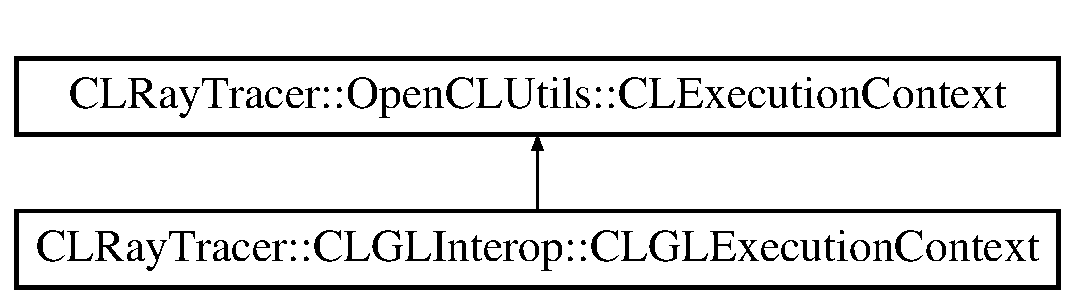
\includegraphics[height=2.000000cm]{class_c_l_ray_tracer_1_1_open_c_l_utils_1_1_c_l_execution_context}
\end{center}
\end{figure}
\subsection*{Public Member Functions}
\begin{DoxyCompactItemize}
\item 
\hyperlink{class_c_l_ray_tracer_1_1_open_c_l_utils_1_1_c_l_execution_context_a4c95e31f2a4dd4127406edbb0ba5edd1}{C\+L\+Execution\+Context} (const \hyperlink{class_c_l_ray_tracer_1_1_open_c_l_utils_1_1_c_l_device}{C\+L\+Device} \&device, const cl\+\_\+context\+\_\+properties $\ast$\+\_\+context\+Properties=N\+U\+LL)
\item 
\hyperlink{_errata_8h_a389396702f1aff6e71eb21328b0775c1}{Common\+::\+Result} \hyperlink{class_c_l_ray_tracer_1_1_open_c_l_utils_1_1_c_l_execution_context_a6b4b2a9f1e8bd3ff516c7bbae4848f61}{initialize} (\hyperlink{class_c_l_ray_tracer_1_1_common_1_1_errata}{Common\+::\+Errata} \&err) const 
\item 
\hyperlink{_errata_8h_a389396702f1aff6e71eb21328b0775c1}{Common\+::\+Result} \hyperlink{class_c_l_ray_tracer_1_1_open_c_l_utils_1_1_c_l_execution_context_a5a953bbfdd89bd898ad2e6ad55c9f634}{create\+Device\+Buffer} (\hyperlink{_c_l_execution_context_8h_a354d4612d8d46b32eb5ad4a71f35694c}{C\+L\+Buffer\+Flags\+::\+C\+L\+Buffer\+Access} access, \hyperlink{_c_l_execution_context_8h_a8e119b9b799e2e980fe86c8e6c93cca6}{C\+L\+Buffer\+Flags\+::\+C\+L\+Buffer\+Host\+Ptr\+Options} host\+Ptr\+Opts, size\+\_\+t size, cl\+\_\+mem \&output, \hyperlink{class_c_l_ray_tracer_1_1_common_1_1_errata}{Common\+::\+Errata} \&err, void $\ast$host\+Ptr=N\+U\+LL) const 
\item 
\hyperlink{_errata_8h_a389396702f1aff6e71eb21328b0775c1}{Common\+::\+Result} \hyperlink{class_c_l_ray_tracer_1_1_open_c_l_utils_1_1_c_l_execution_context_aa8d5e3b745f6c543f2a78c6fd514a79d}{create\+Device\+Buffer} (\hyperlink{_c_l_execution_context_8h_a354d4612d8d46b32eb5ad4a71f35694c}{C\+L\+Buffer\+Flags\+::\+C\+L\+Buffer\+Access} access, size\+\_\+t size, cl\+\_\+mem \&output, \hyperlink{class_c_l_ray_tracer_1_1_common_1_1_errata}{Common\+::\+Errata} \&err) const 
\item 
\hyperlink{_errata_8h_a389396702f1aff6e71eb21328b0775c1}{Common\+::\+Result} \hyperlink{class_c_l_ray_tracer_1_1_open_c_l_utils_1_1_c_l_execution_context_a01b25e47be24d16008b53e5f6431b807}{create\+Event} (boost\+::shared\+\_\+ptr$<$ \hyperlink{class_c_l_ray_tracer_1_1_open_c_l_utils_1_1_c_l_event}{C\+L\+Event} $>$ \&out\+Evt, \hyperlink{class_c_l_ray_tracer_1_1_common_1_1_errata}{Common\+::\+Errata} \&err) const 
\item 
\hyperlink{_errata_8h_a389396702f1aff6e71eb21328b0775c1}{Common\+::\+Result} \hyperlink{class_c_l_ray_tracer_1_1_open_c_l_utils_1_1_c_l_execution_context_a3370232aafe19ac17dc63cee8b8f5e42}{create\+Events} (int count, std\+::vector$<$ boost\+::shared\+\_\+ptr$<$ \hyperlink{class_c_l_ray_tracer_1_1_open_c_l_utils_1_1_c_l_event}{C\+L\+Event} $>$ $>$ \&events, \hyperlink{class_c_l_ray_tracer_1_1_common_1_1_errata}{Common\+::\+Errata} \&err) const 
\item 
\hyperlink{_errata_8h_a389396702f1aff6e71eb21328b0775c1}{Common\+::\+Result} \hyperlink{class_c_l_ray_tracer_1_1_open_c_l_utils_1_1_c_l_execution_context_ac7c1bf6d6ada5d4104e7d96dd0b15b8b}{enqueue\+Read\+Buffer} (const cl\+\_\+mem \&buffer, void $\ast$output\+Buffer, size\+\_\+t buffer\+Size, \hyperlink{class_c_l_ray_tracer_1_1_common_1_1_errata}{Common\+::\+Errata} \&err) const 
\item 
\hyperlink{_errata_8h_a389396702f1aff6e71eb21328b0775c1}{Common\+::\+Result} \hyperlink{class_c_l_ray_tracer_1_1_open_c_l_utils_1_1_c_l_execution_context_a8b5f64a7d034773c60e39a6f280ea9b9}{enqueue\+Read\+Buffer} (const cl\+\_\+mem \&buffer, void $\ast$output\+Buffer, size\+\_\+t offset, size\+\_\+t buffer\+Size, \hyperlink{class_c_l_ray_tracer_1_1_common_1_1_errata}{Common\+::\+Errata} \&err) const 
\item 
\hyperlink{_errata_8h_a389396702f1aff6e71eb21328b0775c1}{Common\+::\+Result} \hyperlink{class_c_l_ray_tracer_1_1_open_c_l_utils_1_1_c_l_execution_context_a091a8577503ecdb380805b2ca7cc2102}{enqueue\+Fill\+Buffer} (const cl\+\_\+mem \&buffer, void $\ast$pattern, size\+\_\+t buffer\+Size, size\+\_\+t pattern\+Size, \hyperlink{class_c_l_ray_tracer_1_1_common_1_1_errata}{Common\+::\+Errata} \&err) const 
\item 
\hyperlink{_errata_8h_a389396702f1aff6e71eb21328b0775c1}{Common\+::\+Result} \hyperlink{class_c_l_ray_tracer_1_1_open_c_l_utils_1_1_c_l_execution_context_a45252fc7bbdf285418220b04abdb135e}{enqueue\+Write\+Buffer} (void $\ast$buffer, const cl\+\_\+mem \&output\+Buffer, size\+\_\+t buffer\+Size, \hyperlink{class_c_l_ray_tracer_1_1_common_1_1_errata}{Common\+::\+Errata} \&err) const 
\item 
\hyperlink{_errata_8h_a389396702f1aff6e71eb21328b0775c1}{Common\+::\+Result} \hyperlink{class_c_l_ray_tracer_1_1_open_c_l_utils_1_1_c_l_execution_context_a1f9900b02109964463ce04ffa29153de}{enqueue\+Copy\+Buffer} (const cl\+\_\+mem \&buffer, const cl\+\_\+mem \&output\+Buffer, size\+\_\+t buffer\+Size, \hyperlink{class_c_l_ray_tracer_1_1_common_1_1_errata}{Common\+::\+Errata} \&err) const 
\item 
\hyperlink{_errata_8h_a389396702f1aff6e71eb21328b0775c1}{Common\+::\+Result} \hyperlink{class_c_l_ray_tracer_1_1_open_c_l_utils_1_1_c_l_execution_context_ab9ac2f839ca431acef0aeb197d17225a}{enqueue\+Kernel} (\hyperlink{class_c_l_ray_tracer_1_1_open_c_l_utils_1_1_c_l_kernel}{C\+L\+Kernel} \&kernel, \hyperlink{class_c_l_ray_tracer_1_1_open_c_l_utils_1_1_c_l_kernel_execute_params}{C\+L\+Kernel\+Execute\+Params} \&params, \hyperlink{class_c_l_ray_tracer_1_1_common_1_1_errata}{Common\+::\+Errata} \&err) const 
\item 
\hyperlink{_errata_8h_a389396702f1aff6e71eb21328b0775c1}{Common\+::\+Result} \hyperlink{class_c_l_ray_tracer_1_1_open_c_l_utils_1_1_c_l_execution_context_a0dbaf20006e360e34ddc52a85246855e}{flush\+Queue} (\hyperlink{class_c_l_ray_tracer_1_1_common_1_1_errata}{Common\+::\+Errata} \&err) const 
\item 
\hyperlink{_errata_8h_a389396702f1aff6e71eb21328b0775c1}{Common\+::\+Result} \hyperlink{class_c_l_ray_tracer_1_1_open_c_l_utils_1_1_c_l_execution_context_a19fb4b24a7d6a184bb5884909761df53}{finish\+Queue} (\hyperlink{class_c_l_ray_tracer_1_1_common_1_1_errata}{Common\+::\+Errata} \&err) const 
\item 
\hyperlink{_errata_8h_a389396702f1aff6e71eb21328b0775c1}{Common\+::\+Result} \hyperlink{class_c_l_ray_tracer_1_1_open_c_l_utils_1_1_c_l_execution_context_a0333381f7772462c72ffbe043d7dfeeb}{get\+Maximal\+Launch\+Exec\+Params} (const \hyperlink{class_c_l_ray_tracer_1_1_open_c_l_utils_1_1_c_l_kernel}{C\+L\+Kernel} \&kernel, size\+\_\+t \&compute\+Devices, size\+\_\+t \&preferred\+Workgroup\+Size, \hyperlink{class_c_l_ray_tracer_1_1_common_1_1_errata}{Common\+::\+Errata} \&err) const 
\item 
\hyperlink{_errata_8h_a389396702f1aff6e71eb21328b0775c1}{Common\+::\+Result} \hyperlink{class_c_l_ray_tracer_1_1_open_c_l_utils_1_1_c_l_execution_context_a16f52f081efa477b9c8f34d28ce272d8}{get\+Max\+Workgroup\+For\+Kernel} (const \hyperlink{class_c_l_ray_tracer_1_1_open_c_l_utils_1_1_c_l_kernel}{C\+L\+Kernel} \&kernel, size\+\_\+t \&max\+W\+G\+Size, \hyperlink{class_c_l_ray_tracer_1_1_common_1_1_errata}{Common\+::\+Errata} \&err) const 
\item 
const \hyperlink{class_c_l_ray_tracer_1_1_open_c_l_utils_1_1_c_l_device}{C\+L\+Device} \& \hyperlink{class_c_l_ray_tracer_1_1_open_c_l_utils_1_1_c_l_execution_context_afa781473cfa153504e5efbf2208faa99}{get\+Device} () const 
\item 
virtual \hyperlink{class_c_l_ray_tracer_1_1_open_c_l_utils_1_1_c_l_execution_context_aa06c0a22a6f773ccca68d4ca5c51704d}{$\sim$\+C\+L\+Execution\+Context} ()
\end{DoxyCompactItemize}
\subsection*{Protected Attributes}
\begin{DoxyCompactItemize}
\item 
const \hyperlink{class_c_l_ray_tracer_1_1_open_c_l_utils_1_1_c_l_platform}{C\+L\+Platform} \& {\bfseries \+\_\+platform}\hypertarget{class_c_l_ray_tracer_1_1_open_c_l_utils_1_1_c_l_execution_context_ad34dd30602a4379d71eaa4626a5633c7}{}\label{class_c_l_ray_tracer_1_1_open_c_l_utils_1_1_c_l_execution_context_ad34dd30602a4379d71eaa4626a5633c7}

\item 
const \hyperlink{class_c_l_ray_tracer_1_1_open_c_l_utils_1_1_c_l_device}{C\+L\+Device} \& {\bfseries \+\_\+device}\hypertarget{class_c_l_ray_tracer_1_1_open_c_l_utils_1_1_c_l_execution_context_ab427e8d09a800f1acc361852df128e55}{}\label{class_c_l_ray_tracer_1_1_open_c_l_utils_1_1_c_l_execution_context_ab427e8d09a800f1acc361852df128e55}

\item 
const cl\+\_\+context\+\_\+properties $\ast$ {\bfseries \+\_\+context\+Properties}\hypertarget{class_c_l_ray_tracer_1_1_open_c_l_utils_1_1_c_l_execution_context_a4971df1c7754dda8244afbc22693e6d5}{}\label{class_c_l_ray_tracer_1_1_open_c_l_utils_1_1_c_l_execution_context_a4971df1c7754dda8244afbc22693e6d5}

\item 
cl\+\_\+context {\bfseries \+\_\+cl\+Context}\hypertarget{class_c_l_ray_tracer_1_1_open_c_l_utils_1_1_c_l_execution_context_a6631dc137a2ac7ca7534581949c743f5}{}\label{class_c_l_ray_tracer_1_1_open_c_l_utils_1_1_c_l_execution_context_a6631dc137a2ac7ca7534581949c743f5}

\item 
cl\+\_\+command\+\_\+queue {\bfseries \+\_\+cl\+Command\+Queue}\hypertarget{class_c_l_ray_tracer_1_1_open_c_l_utils_1_1_c_l_execution_context_a0e8a021bab04d399b9c8abfb02f46353}{}\label{class_c_l_ray_tracer_1_1_open_c_l_utils_1_1_c_l_execution_context_a0e8a021bab04d399b9c8abfb02f46353}

\item 
bool {\bfseries \+\_\+initialized}\hypertarget{class_c_l_ray_tracer_1_1_open_c_l_utils_1_1_c_l_execution_context_a98b83d0951e39eb57c44c6fcd30f5f63}{}\label{class_c_l_ray_tracer_1_1_open_c_l_utils_1_1_c_l_execution_context_a98b83d0951e39eb57c44c6fcd30f5f63}

\end{DoxyCompactItemize}
\subsection*{Friends}
\begin{DoxyCompactItemize}
\item 
class {\bfseries C\+L\+Program}\hypertarget{class_c_l_ray_tracer_1_1_open_c_l_utils_1_1_c_l_execution_context_a5a2118afd420ad2f664e518740aa1e5d}{}\label{class_c_l_ray_tracer_1_1_open_c_l_utils_1_1_c_l_execution_context_a5a2118afd420ad2f664e518740aa1e5d}

\end{DoxyCompactItemize}


\subsection{Detailed Description}
class \hyperlink{class_c_l_ray_tracer_1_1_open_c_l_utils_1_1_c_l_execution_context}{C\+L\+Execution\+Context} encapsulates operations on Open\+CL command queue\+: Kernel executions, memory operations, creating synchronization events, etc. This class encapsulates partial set of those operations, and can be extended if needed 

\subsection{Constructor \& Destructor Documentation}
\index{C\+L\+Ray\+Tracer\+::\+Open\+C\+L\+Utils\+::\+C\+L\+Execution\+Context@{C\+L\+Ray\+Tracer\+::\+Open\+C\+L\+Utils\+::\+C\+L\+Execution\+Context}!C\+L\+Execution\+Context@{C\+L\+Execution\+Context}}
\index{C\+L\+Execution\+Context@{C\+L\+Execution\+Context}!C\+L\+Ray\+Tracer\+::\+Open\+C\+L\+Utils\+::\+C\+L\+Execution\+Context@{C\+L\+Ray\+Tracer\+::\+Open\+C\+L\+Utils\+::\+C\+L\+Execution\+Context}}
\subsubsection[{\texorpdfstring{C\+L\+Execution\+Context(const C\+L\+Device \&device, const cl\+\_\+context\+\_\+properties $\ast$\+\_\+context\+Properties=\+N\+U\+L\+L)}{CLExecutionContext(const CLDevice &device, const cl_context_properties *_contextProperties=NULL)}}]{\setlength{\rightskip}{0pt plus 5cm}C\+L\+Ray\+Tracer\+::\+Open\+C\+L\+Utils\+::\+C\+L\+Execution\+Context\+::\+C\+L\+Execution\+Context (
\begin{DoxyParamCaption}
\item[{const {\bf C\+L\+Device} \&}]{device, }
\item[{const cl\+\_\+context\+\_\+properties $\ast$}]{\+\_\+context\+Properties = {\ttfamily NULL}}
\end{DoxyParamCaption}
)}\hypertarget{class_c_l_ray_tracer_1_1_open_c_l_utils_1_1_c_l_execution_context_a4c95e31f2a4dd4127406edbb0ba5edd1}{}\label{class_c_l_ray_tracer_1_1_open_c_l_utils_1_1_c_l_execution_context_a4c95e31f2a4dd4127406edbb0ba5edd1}
Constructor 
\begin{DoxyParams}{Parameters}
{\em device} & Object that encapsulate the Open\+CL device in use \\
\hline
{\em context\+Properties\mbox{[}optional\mbox{]}} & The properties of context to be created \\
\hline
\end{DoxyParams}
\begin{DoxySeeAlso}{See also}
class \hyperlink{class_c_l_ray_tracer_1_1_open_c_l_utils_1_1_c_l_device}{C\+L\+Device} 

cl\+\_\+context\+\_\+properties in Open\+CL specification 
\end{DoxySeeAlso}
\index{C\+L\+Ray\+Tracer\+::\+Open\+C\+L\+Utils\+::\+C\+L\+Execution\+Context@{C\+L\+Ray\+Tracer\+::\+Open\+C\+L\+Utils\+::\+C\+L\+Execution\+Context}!````~C\+L\+Execution\+Context@{$\sim$\+C\+L\+Execution\+Context}}
\index{````~C\+L\+Execution\+Context@{$\sim$\+C\+L\+Execution\+Context}!C\+L\+Ray\+Tracer\+::\+Open\+C\+L\+Utils\+::\+C\+L\+Execution\+Context@{C\+L\+Ray\+Tracer\+::\+Open\+C\+L\+Utils\+::\+C\+L\+Execution\+Context}}
\subsubsection[{\texorpdfstring{$\sim$\+C\+L\+Execution\+Context()}{~CLExecutionContext()}}]{\setlength{\rightskip}{0pt plus 5cm}virtual C\+L\+Ray\+Tracer\+::\+Open\+C\+L\+Utils\+::\+C\+L\+Execution\+Context\+::$\sim$\+C\+L\+Execution\+Context (
\begin{DoxyParamCaption}
{}
\end{DoxyParamCaption}
)\hspace{0.3cm}{\ttfamily [virtual]}}\hypertarget{class_c_l_ray_tracer_1_1_open_c_l_utils_1_1_c_l_execution_context_aa06c0a22a6f773ccca68d4ca5c51704d}{}\label{class_c_l_ray_tracer_1_1_open_c_l_utils_1_1_c_l_execution_context_aa06c0a22a6f773ccca68d4ca5c51704d}
Destructor 

\subsection{Member Function Documentation}
\index{C\+L\+Ray\+Tracer\+::\+Open\+C\+L\+Utils\+::\+C\+L\+Execution\+Context@{C\+L\+Ray\+Tracer\+::\+Open\+C\+L\+Utils\+::\+C\+L\+Execution\+Context}!create\+Device\+Buffer@{create\+Device\+Buffer}}
\index{create\+Device\+Buffer@{create\+Device\+Buffer}!C\+L\+Ray\+Tracer\+::\+Open\+C\+L\+Utils\+::\+C\+L\+Execution\+Context@{C\+L\+Ray\+Tracer\+::\+Open\+C\+L\+Utils\+::\+C\+L\+Execution\+Context}}
\subsubsection[{\texorpdfstring{create\+Device\+Buffer(\+C\+L\+Buffer\+Flags\+::\+C\+L\+Buffer\+Access access, C\+L\+Buffer\+Flags\+::\+C\+L\+Buffer\+Host\+Ptr\+Options host\+Ptr\+Opts, size\+\_\+t size, cl\+\_\+mem \&output, Common\+::\+Errata \&err, void $\ast$host\+Ptr=\+N\+U\+L\+L) const }{createDeviceBuffer(CLBufferFlags::CLBufferAccess access, CLBufferFlags::CLBufferHostPtrOptions hostPtrOpts, size_t size, cl_mem &output, Common::Errata &err, void *hostPtr=NULL) const }}]{\setlength{\rightskip}{0pt plus 5cm}{\bf Common\+::\+Result} C\+L\+Ray\+Tracer\+::\+Open\+C\+L\+Utils\+::\+C\+L\+Execution\+Context\+::create\+Device\+Buffer (
\begin{DoxyParamCaption}
\item[{{\bf C\+L\+Buffer\+Flags\+::\+C\+L\+Buffer\+Access}}]{access, }
\item[{{\bf C\+L\+Buffer\+Flags\+::\+C\+L\+Buffer\+Host\+Ptr\+Options}}]{host\+Ptr\+Opts, }
\item[{size\+\_\+t}]{size, }
\item[{cl\+\_\+mem \&}]{output, }
\item[{{\bf Common\+::\+Errata} \&}]{err, }
\item[{void $\ast$}]{host\+Ptr = {\ttfamily NULL}}
\end{DoxyParamCaption}
) const}\hypertarget{class_c_l_ray_tracer_1_1_open_c_l_utils_1_1_c_l_execution_context_a5a953bbfdd89bd898ad2e6ad55c9f634}{}\label{class_c_l_ray_tracer_1_1_open_c_l_utils_1_1_c_l_execution_context_a5a953bbfdd89bd898ad2e6ad55c9f634}
Create Open\+CL memory object 
\begin{DoxyParams}[1]{Parameters}
 & {\em access} & Access mode \\
\hline
 & {\em host\+Ptr\+Opts} & Host pointer usage \\
\hline
 & {\em size} & Desired size of the buffer \\
\hline
\mbox{\tt out}  & {\em } & \\
\hline
\end{DoxyParams}
\index{C\+L\+Ray\+Tracer\+::\+Open\+C\+L\+Utils\+::\+C\+L\+Execution\+Context@{C\+L\+Ray\+Tracer\+::\+Open\+C\+L\+Utils\+::\+C\+L\+Execution\+Context}!create\+Device\+Buffer@{create\+Device\+Buffer}}
\index{create\+Device\+Buffer@{create\+Device\+Buffer}!C\+L\+Ray\+Tracer\+::\+Open\+C\+L\+Utils\+::\+C\+L\+Execution\+Context@{C\+L\+Ray\+Tracer\+::\+Open\+C\+L\+Utils\+::\+C\+L\+Execution\+Context}}
\subsubsection[{\texorpdfstring{create\+Device\+Buffer(\+C\+L\+Buffer\+Flags\+::\+C\+L\+Buffer\+Access access, size\+\_\+t size, cl\+\_\+mem \&output, Common\+::\+Errata \&err) const }{createDeviceBuffer(CLBufferFlags::CLBufferAccess access, size_t size, cl_mem &output, Common::Errata &err) const }}]{\setlength{\rightskip}{0pt plus 5cm}{\bf Common\+::\+Result} C\+L\+Ray\+Tracer\+::\+Open\+C\+L\+Utils\+::\+C\+L\+Execution\+Context\+::create\+Device\+Buffer (
\begin{DoxyParamCaption}
\item[{{\bf C\+L\+Buffer\+Flags\+::\+C\+L\+Buffer\+Access}}]{access, }
\item[{size\+\_\+t}]{size, }
\item[{cl\+\_\+mem \&}]{output, }
\item[{{\bf Common\+::\+Errata} \&}]{err}
\end{DoxyParamCaption}
) const}\hypertarget{class_c_l_ray_tracer_1_1_open_c_l_utils_1_1_c_l_execution_context_aa8d5e3b745f6c543f2a78c6fd514a79d}{}\label{class_c_l_ray_tracer_1_1_open_c_l_utils_1_1_c_l_execution_context_aa8d5e3b745f6c543f2a78c6fd514a79d}
Create Open\+CL memory object 
\begin{DoxyParams}[1]{Parameters}
 & {\em access} & Access mode \\
\hline
 & {\em size} & Desired size of the buffer \\
\hline
\mbox{\tt out}  & {\em } & \\
\hline
\end{DoxyParams}
\index{C\+L\+Ray\+Tracer\+::\+Open\+C\+L\+Utils\+::\+C\+L\+Execution\+Context@{C\+L\+Ray\+Tracer\+::\+Open\+C\+L\+Utils\+::\+C\+L\+Execution\+Context}!create\+Event@{create\+Event}}
\index{create\+Event@{create\+Event}!C\+L\+Ray\+Tracer\+::\+Open\+C\+L\+Utils\+::\+C\+L\+Execution\+Context@{C\+L\+Ray\+Tracer\+::\+Open\+C\+L\+Utils\+::\+C\+L\+Execution\+Context}}
\subsubsection[{\texorpdfstring{create\+Event(boost\+::shared\+\_\+ptr$<$ C\+L\+Event $>$ \&out\+Evt, Common\+::\+Errata \&err) const }{createEvent(boost::shared_ptr< CLEvent > &outEvt, Common::Errata &err) const }}]{\setlength{\rightskip}{0pt plus 5cm}{\bf Common\+::\+Result} C\+L\+Ray\+Tracer\+::\+Open\+C\+L\+Utils\+::\+C\+L\+Execution\+Context\+::create\+Event (
\begin{DoxyParamCaption}
\item[{boost\+::shared\+\_\+ptr$<$ {\bf C\+L\+Event} $>$ \&}]{out\+Evt, }
\item[{{\bf Common\+::\+Errata} \&}]{err}
\end{DoxyParamCaption}
) const}\hypertarget{class_c_l_ray_tracer_1_1_open_c_l_utils_1_1_c_l_execution_context_a01b25e47be24d16008b53e5f6431b807}{}\label{class_c_l_ray_tracer_1_1_open_c_l_utils_1_1_c_l_execution_context_a01b25e47be24d16008b53e5f6431b807}
Creates object that encapsulates Open\+CL synchronization event 
\begin{DoxyParams}[1]{Parameters}
\mbox{\tt out}  & {\em } & \\
\hline
\end{DoxyParams}
\index{C\+L\+Ray\+Tracer\+::\+Open\+C\+L\+Utils\+::\+C\+L\+Execution\+Context@{C\+L\+Ray\+Tracer\+::\+Open\+C\+L\+Utils\+::\+C\+L\+Execution\+Context}!create\+Events@{create\+Events}}
\index{create\+Events@{create\+Events}!C\+L\+Ray\+Tracer\+::\+Open\+C\+L\+Utils\+::\+C\+L\+Execution\+Context@{C\+L\+Ray\+Tracer\+::\+Open\+C\+L\+Utils\+::\+C\+L\+Execution\+Context}}
\subsubsection[{\texorpdfstring{create\+Events(int count, std\+::vector$<$ boost\+::shared\+\_\+ptr$<$ C\+L\+Event $>$ $>$ \&events, Common\+::\+Errata \&err) const }{createEvents(int count, std::vector< boost::shared_ptr< CLEvent > > &events, Common::Errata &err) const }}]{\setlength{\rightskip}{0pt plus 5cm}{\bf Common\+::\+Result} C\+L\+Ray\+Tracer\+::\+Open\+C\+L\+Utils\+::\+C\+L\+Execution\+Context\+::create\+Events (
\begin{DoxyParamCaption}
\item[{int}]{count, }
\item[{std\+::vector$<$ boost\+::shared\+\_\+ptr$<$ {\bf C\+L\+Event} $>$ $>$ \&}]{events, }
\item[{{\bf Common\+::\+Errata} \&}]{err}
\end{DoxyParamCaption}
) const}\hypertarget{class_c_l_ray_tracer_1_1_open_c_l_utils_1_1_c_l_execution_context_a3370232aafe19ac17dc63cee8b8f5e42}{}\label{class_c_l_ray_tracer_1_1_open_c_l_utils_1_1_c_l_execution_context_a3370232aafe19ac17dc63cee8b8f5e42}
Creates multiple objects that encapsulates Open\+CL synchronization event 
\begin{DoxyParams}{Parameters}
{\em count} & Count of desired events \\
\hline
{\em events} & Vector that shall be filled with created events \\
\hline
{\em err} & Error info \\
\hline
\end{DoxyParams}
\begin{DoxyReturn}{Returns}
Result of the operation\+: Success or failure 
\end{DoxyReturn}
\index{C\+L\+Ray\+Tracer\+::\+Open\+C\+L\+Utils\+::\+C\+L\+Execution\+Context@{C\+L\+Ray\+Tracer\+::\+Open\+C\+L\+Utils\+::\+C\+L\+Execution\+Context}!enqueue\+Copy\+Buffer@{enqueue\+Copy\+Buffer}}
\index{enqueue\+Copy\+Buffer@{enqueue\+Copy\+Buffer}!C\+L\+Ray\+Tracer\+::\+Open\+C\+L\+Utils\+::\+C\+L\+Execution\+Context@{C\+L\+Ray\+Tracer\+::\+Open\+C\+L\+Utils\+::\+C\+L\+Execution\+Context}}
\subsubsection[{\texorpdfstring{enqueue\+Copy\+Buffer(const cl\+\_\+mem \&buffer, const cl\+\_\+mem \&output\+Buffer, size\+\_\+t buffer\+Size, Common\+::\+Errata \&err) const }{enqueueCopyBuffer(const cl_mem &buffer, const cl_mem &outputBuffer, size_t bufferSize, Common::Errata &err) const }}]{\setlength{\rightskip}{0pt plus 5cm}{\bf Common\+::\+Result} C\+L\+Ray\+Tracer\+::\+Open\+C\+L\+Utils\+::\+C\+L\+Execution\+Context\+::enqueue\+Copy\+Buffer (
\begin{DoxyParamCaption}
\item[{const cl\+\_\+mem \&}]{buffer, }
\item[{const cl\+\_\+mem \&}]{output\+Buffer, }
\item[{size\+\_\+t}]{buffer\+Size, }
\item[{{\bf Common\+::\+Errata} \&}]{err}
\end{DoxyParamCaption}
) const}\hypertarget{class_c_l_ray_tracer_1_1_open_c_l_utils_1_1_c_l_execution_context_a1f9900b02109964463ce04ffa29153de}{}\label{class_c_l_ray_tracer_1_1_open_c_l_utils_1_1_c_l_execution_context_a1f9900b02109964463ce04ffa29153de}
Copies Open\+CL device memory into destination memory on device 
\begin{DoxyParams}{Parameters}
{\em buffer} & Source Open\+CL device buffer \\
\hline
{\em output\+Buffer} & Destination Open\+CL device buffer \\
\hline
{\em buffer\+Size} & The size of the buffer that should be copied \\
\hline
{\em err} & Error info \\
\hline
\end{DoxyParams}
\begin{DoxyReturn}{Returns}
Result of the operation\+: Success or failure 
\end{DoxyReturn}
\index{C\+L\+Ray\+Tracer\+::\+Open\+C\+L\+Utils\+::\+C\+L\+Execution\+Context@{C\+L\+Ray\+Tracer\+::\+Open\+C\+L\+Utils\+::\+C\+L\+Execution\+Context}!enqueue\+Fill\+Buffer@{enqueue\+Fill\+Buffer}}
\index{enqueue\+Fill\+Buffer@{enqueue\+Fill\+Buffer}!C\+L\+Ray\+Tracer\+::\+Open\+C\+L\+Utils\+::\+C\+L\+Execution\+Context@{C\+L\+Ray\+Tracer\+::\+Open\+C\+L\+Utils\+::\+C\+L\+Execution\+Context}}
\subsubsection[{\texorpdfstring{enqueue\+Fill\+Buffer(const cl\+\_\+mem \&buffer, void $\ast$pattern, size\+\_\+t buffer\+Size, size\+\_\+t pattern\+Size, Common\+::\+Errata \&err) const }{enqueueFillBuffer(const cl_mem &buffer, void *pattern, size_t bufferSize, size_t patternSize, Common::Errata &err) const }}]{\setlength{\rightskip}{0pt plus 5cm}{\bf Common\+::\+Result} C\+L\+Ray\+Tracer\+::\+Open\+C\+L\+Utils\+::\+C\+L\+Execution\+Context\+::enqueue\+Fill\+Buffer (
\begin{DoxyParamCaption}
\item[{const cl\+\_\+mem \&}]{buffer, }
\item[{void $\ast$}]{pattern, }
\item[{size\+\_\+t}]{buffer\+Size, }
\item[{size\+\_\+t}]{pattern\+Size, }
\item[{{\bf Common\+::\+Errata} \&}]{err}
\end{DoxyParamCaption}
) const}\hypertarget{class_c_l_ray_tracer_1_1_open_c_l_utils_1_1_c_l_execution_context_a091a8577503ecdb380805b2ca7cc2102}{}\label{class_c_l_ray_tracer_1_1_open_c_l_utils_1_1_c_l_execution_context_a091a8577503ecdb380805b2ca7cc2102}
Fills Open\+CL device memory with defined pattern, same principle as Win32 memset 
\begin{DoxyParams}{Parameters}
{\em buffer} & Open\+CL device buffer \\
\hline
{\em pattern} & The pattern that should be filled \\
\hline
{\em buffer\+Size} & The size of the buffer that should be copied. Must be a multiple of pattern\+Size \\
\hline
{\em pattern\+Size} & pattern\+Size The size of pattern -\/ According to Open\+CL specs can be \{1, 2, 4, 8, 16, 32, 64, 128\} \\
\hline
{\em err} & Error info \\
\hline
\end{DoxyParams}
\begin{DoxyReturn}{Returns}
Result of the operation\+: Success or failure 
\end{DoxyReturn}
\index{C\+L\+Ray\+Tracer\+::\+Open\+C\+L\+Utils\+::\+C\+L\+Execution\+Context@{C\+L\+Ray\+Tracer\+::\+Open\+C\+L\+Utils\+::\+C\+L\+Execution\+Context}!enqueue\+Kernel@{enqueue\+Kernel}}
\index{enqueue\+Kernel@{enqueue\+Kernel}!C\+L\+Ray\+Tracer\+::\+Open\+C\+L\+Utils\+::\+C\+L\+Execution\+Context@{C\+L\+Ray\+Tracer\+::\+Open\+C\+L\+Utils\+::\+C\+L\+Execution\+Context}}
\subsubsection[{\texorpdfstring{enqueue\+Kernel(\+C\+L\+Kernel \&kernel, C\+L\+Kernel\+Execute\+Params \&params, Common\+::\+Errata \&err) const }{enqueueKernel(CLKernel &kernel, CLKernelExecuteParams &params, Common::Errata &err) const }}]{\setlength{\rightskip}{0pt plus 5cm}{\bf Common\+::\+Result} C\+L\+Ray\+Tracer\+::\+Open\+C\+L\+Utils\+::\+C\+L\+Execution\+Context\+::enqueue\+Kernel (
\begin{DoxyParamCaption}
\item[{{\bf C\+L\+Kernel} \&}]{kernel, }
\item[{{\bf C\+L\+Kernel\+Execute\+Params} \&}]{params, }
\item[{{\bf Common\+::\+Errata} \&}]{err}
\end{DoxyParamCaption}
) const}\hypertarget{class_c_l_ray_tracer_1_1_open_c_l_utils_1_1_c_l_execution_context_ab9ac2f839ca431acef0aeb197d17225a}{}\label{class_c_l_ray_tracer_1_1_open_c_l_utils_1_1_c_l_execution_context_ab9ac2f839ca431acef0aeb197d17225a}
Enqueues kernel execution on underlying Open\+CL command queue -\/ In simple terms, executes the kernel 
\begin{DoxyParams}{Parameters}
{\em Object} & that encapsulates the kernel to execute \\
\hline
{\em Object} & that encapsulates data about dimensions and syncronization events for kernel execution \\
\hline
{\em err} & Error info \\
\hline
\end{DoxyParams}
\begin{DoxyReturn}{Returns}
Result of the operation\+: Success or failure 
\end{DoxyReturn}
\index{C\+L\+Ray\+Tracer\+::\+Open\+C\+L\+Utils\+::\+C\+L\+Execution\+Context@{C\+L\+Ray\+Tracer\+::\+Open\+C\+L\+Utils\+::\+C\+L\+Execution\+Context}!enqueue\+Read\+Buffer@{enqueue\+Read\+Buffer}}
\index{enqueue\+Read\+Buffer@{enqueue\+Read\+Buffer}!C\+L\+Ray\+Tracer\+::\+Open\+C\+L\+Utils\+::\+C\+L\+Execution\+Context@{C\+L\+Ray\+Tracer\+::\+Open\+C\+L\+Utils\+::\+C\+L\+Execution\+Context}}
\subsubsection[{\texorpdfstring{enqueue\+Read\+Buffer(const cl\+\_\+mem \&buffer, void $\ast$output\+Buffer, size\+\_\+t buffer\+Size, Common\+::\+Errata \&err) const }{enqueueReadBuffer(const cl_mem &buffer, void *outputBuffer, size_t bufferSize, Common::Errata &err) const }}]{\setlength{\rightskip}{0pt plus 5cm}{\bf Common\+::\+Result} C\+L\+Ray\+Tracer\+::\+Open\+C\+L\+Utils\+::\+C\+L\+Execution\+Context\+::enqueue\+Read\+Buffer (
\begin{DoxyParamCaption}
\item[{const cl\+\_\+mem \&}]{buffer, }
\item[{void $\ast$}]{output\+Buffer, }
\item[{size\+\_\+t}]{buffer\+Size, }
\item[{{\bf Common\+::\+Errata} \&}]{err}
\end{DoxyParamCaption}
) const}\hypertarget{class_c_l_ray_tracer_1_1_open_c_l_utils_1_1_c_l_execution_context_ac7c1bf6d6ada5d4104e7d96dd0b15b8b}{}\label{class_c_l_ray_tracer_1_1_open_c_l_utils_1_1_c_l_execution_context_ac7c1bf6d6ada5d4104e7d96dd0b15b8b}
Reads Open\+CL device memory contents and writes them into host memory buffer 
\begin{DoxyParams}{Parameters}
{\em buffer} & Open\+CL device buffer \\
\hline
{\em output\+Buffer} & Host memory pointer to destination, where memory should be copied \\
\hline
{\em buffer\+Size} & The size of the buffer that should be copied \\
\hline
{\em err} & Error info \\
\hline
\end{DoxyParams}
\begin{DoxyReturn}{Returns}
Result of the operation\+: Success or failure 
\end{DoxyReturn}
\index{C\+L\+Ray\+Tracer\+::\+Open\+C\+L\+Utils\+::\+C\+L\+Execution\+Context@{C\+L\+Ray\+Tracer\+::\+Open\+C\+L\+Utils\+::\+C\+L\+Execution\+Context}!enqueue\+Read\+Buffer@{enqueue\+Read\+Buffer}}
\index{enqueue\+Read\+Buffer@{enqueue\+Read\+Buffer}!C\+L\+Ray\+Tracer\+::\+Open\+C\+L\+Utils\+::\+C\+L\+Execution\+Context@{C\+L\+Ray\+Tracer\+::\+Open\+C\+L\+Utils\+::\+C\+L\+Execution\+Context}}
\subsubsection[{\texorpdfstring{enqueue\+Read\+Buffer(const cl\+\_\+mem \&buffer, void $\ast$output\+Buffer, size\+\_\+t offset, size\+\_\+t buffer\+Size, Common\+::\+Errata \&err) const }{enqueueReadBuffer(const cl_mem &buffer, void *outputBuffer, size_t offset, size_t bufferSize, Common::Errata &err) const }}]{\setlength{\rightskip}{0pt plus 5cm}{\bf Common\+::\+Result} C\+L\+Ray\+Tracer\+::\+Open\+C\+L\+Utils\+::\+C\+L\+Execution\+Context\+::enqueue\+Read\+Buffer (
\begin{DoxyParamCaption}
\item[{const cl\+\_\+mem \&}]{buffer, }
\item[{void $\ast$}]{output\+Buffer, }
\item[{size\+\_\+t}]{offset, }
\item[{size\+\_\+t}]{buffer\+Size, }
\item[{{\bf Common\+::\+Errata} \&}]{err}
\end{DoxyParamCaption}
) const}\hypertarget{class_c_l_ray_tracer_1_1_open_c_l_utils_1_1_c_l_execution_context_a8b5f64a7d034773c60e39a6f280ea9b9}{}\label{class_c_l_ray_tracer_1_1_open_c_l_utils_1_1_c_l_execution_context_a8b5f64a7d034773c60e39a6f280ea9b9}
Reads Open\+CL device memory contents and writes them into host memory buffer 
\begin{DoxyParams}{Parameters}
{\em buffer} & Open\+CL device buffer \\
\hline
{\em output\+Buffer} & Host memory pointer to destination, where memory should be copied \\
\hline
{\em offset} & Offset index (In bytes), from which the copying should start \\
\hline
{\em buffer\+Size} & The size of the buffer that should be copied \\
\hline
{\em err} & Error info \\
\hline
\end{DoxyParams}
\begin{DoxyReturn}{Returns}
Result of the operation\+: Success or failure 
\end{DoxyReturn}
\index{C\+L\+Ray\+Tracer\+::\+Open\+C\+L\+Utils\+::\+C\+L\+Execution\+Context@{C\+L\+Ray\+Tracer\+::\+Open\+C\+L\+Utils\+::\+C\+L\+Execution\+Context}!enqueue\+Write\+Buffer@{enqueue\+Write\+Buffer}}
\index{enqueue\+Write\+Buffer@{enqueue\+Write\+Buffer}!C\+L\+Ray\+Tracer\+::\+Open\+C\+L\+Utils\+::\+C\+L\+Execution\+Context@{C\+L\+Ray\+Tracer\+::\+Open\+C\+L\+Utils\+::\+C\+L\+Execution\+Context}}
\subsubsection[{\texorpdfstring{enqueue\+Write\+Buffer(void $\ast$buffer, const cl\+\_\+mem \&output\+Buffer, size\+\_\+t buffer\+Size, Common\+::\+Errata \&err) const }{enqueueWriteBuffer(void *buffer, const cl_mem &outputBuffer, size_t bufferSize, Common::Errata &err) const }}]{\setlength{\rightskip}{0pt plus 5cm}{\bf Common\+::\+Result} C\+L\+Ray\+Tracer\+::\+Open\+C\+L\+Utils\+::\+C\+L\+Execution\+Context\+::enqueue\+Write\+Buffer (
\begin{DoxyParamCaption}
\item[{void $\ast$}]{buffer, }
\item[{const cl\+\_\+mem \&}]{output\+Buffer, }
\item[{size\+\_\+t}]{buffer\+Size, }
\item[{{\bf Common\+::\+Errata} \&}]{err}
\end{DoxyParamCaption}
) const}\hypertarget{class_c_l_ray_tracer_1_1_open_c_l_utils_1_1_c_l_execution_context_a45252fc7bbdf285418220b04abdb135e}{}\label{class_c_l_ray_tracer_1_1_open_c_l_utils_1_1_c_l_execution_context_a45252fc7bbdf285418220b04abdb135e}
Fills Open\+CL device memory with contents of host memory buffer 
\begin{DoxyParams}{Parameters}
{\em buffer} & Host buffer -\/ The source \\
\hline
{\em output\+Buffer} & Open\+CL device buffer -\/ The destination \\
\hline
{\em buffer\+Size} & The size of the buffer that should be copied \\
\hline
{\em err} & Error info \\
\hline
\end{DoxyParams}
\begin{DoxyReturn}{Returns}
Result of the operation\+: Success or failure 
\end{DoxyReturn}
\index{C\+L\+Ray\+Tracer\+::\+Open\+C\+L\+Utils\+::\+C\+L\+Execution\+Context@{C\+L\+Ray\+Tracer\+::\+Open\+C\+L\+Utils\+::\+C\+L\+Execution\+Context}!finish\+Queue@{finish\+Queue}}
\index{finish\+Queue@{finish\+Queue}!C\+L\+Ray\+Tracer\+::\+Open\+C\+L\+Utils\+::\+C\+L\+Execution\+Context@{C\+L\+Ray\+Tracer\+::\+Open\+C\+L\+Utils\+::\+C\+L\+Execution\+Context}}
\subsubsection[{\texorpdfstring{finish\+Queue(\+Common\+::\+Errata \&err) const }{finishQueue(Common::Errata &err) const }}]{\setlength{\rightskip}{0pt plus 5cm}{\bf Common\+::\+Result} C\+L\+Ray\+Tracer\+::\+Open\+C\+L\+Utils\+::\+C\+L\+Execution\+Context\+::finish\+Queue (
\begin{DoxyParamCaption}
\item[{{\bf Common\+::\+Errata} \&}]{err}
\end{DoxyParamCaption}
) const}\hypertarget{class_c_l_ray_tracer_1_1_open_c_l_utils_1_1_c_l_execution_context_a19fb4b24a7d6a184bb5884909761df53}{}\label{class_c_l_ray_tracer_1_1_open_c_l_utils_1_1_c_l_execution_context_a19fb4b24a7d6a184bb5884909761df53}
Blocks until all commands on the queue are completed. Encapsulates the cl\+Finish Open\+CL method 
\begin{DoxyParams}{Parameters}
{\em err} & Error info \\
\hline
\end{DoxyParams}
\begin{DoxyReturn}{Returns}
Result of the operation\+: Success or failure 
\end{DoxyReturn}
\begin{DoxySeeAlso}{See also}
cl\+Finish 
\end{DoxySeeAlso}
\index{C\+L\+Ray\+Tracer\+::\+Open\+C\+L\+Utils\+::\+C\+L\+Execution\+Context@{C\+L\+Ray\+Tracer\+::\+Open\+C\+L\+Utils\+::\+C\+L\+Execution\+Context}!flush\+Queue@{flush\+Queue}}
\index{flush\+Queue@{flush\+Queue}!C\+L\+Ray\+Tracer\+::\+Open\+C\+L\+Utils\+::\+C\+L\+Execution\+Context@{C\+L\+Ray\+Tracer\+::\+Open\+C\+L\+Utils\+::\+C\+L\+Execution\+Context}}
\subsubsection[{\texorpdfstring{flush\+Queue(\+Common\+::\+Errata \&err) const }{flushQueue(Common::Errata &err) const }}]{\setlength{\rightskip}{0pt plus 5cm}{\bf Common\+::\+Result} C\+L\+Ray\+Tracer\+::\+Open\+C\+L\+Utils\+::\+C\+L\+Execution\+Context\+::flush\+Queue (
\begin{DoxyParamCaption}
\item[{{\bf Common\+::\+Errata} \&}]{err}
\end{DoxyParamCaption}
) const}\hypertarget{class_c_l_ray_tracer_1_1_open_c_l_utils_1_1_c_l_execution_context_a0dbaf20006e360e34ddc52a85246855e}{}\label{class_c_l_ray_tracer_1_1_open_c_l_utils_1_1_c_l_execution_context_a0dbaf20006e360e34ddc52a85246855e}
Issues all queues operations to the device. Encapsulates the cl\+Flush Open\+CL method 
\begin{DoxyParams}{Parameters}
{\em err} & Error info \\
\hline
\end{DoxyParams}
\begin{DoxyReturn}{Returns}
Result of the operation\+: Success or failure 
\end{DoxyReturn}
\begin{DoxySeeAlso}{See also}
cl\+Flush 
\end{DoxySeeAlso}
\index{C\+L\+Ray\+Tracer\+::\+Open\+C\+L\+Utils\+::\+C\+L\+Execution\+Context@{C\+L\+Ray\+Tracer\+::\+Open\+C\+L\+Utils\+::\+C\+L\+Execution\+Context}!get\+Device@{get\+Device}}
\index{get\+Device@{get\+Device}!C\+L\+Ray\+Tracer\+::\+Open\+C\+L\+Utils\+::\+C\+L\+Execution\+Context@{C\+L\+Ray\+Tracer\+::\+Open\+C\+L\+Utils\+::\+C\+L\+Execution\+Context}}
\subsubsection[{\texorpdfstring{get\+Device() const }{getDevice() const }}]{\setlength{\rightskip}{0pt plus 5cm}const {\bf C\+L\+Device}\& C\+L\+Ray\+Tracer\+::\+Open\+C\+L\+Utils\+::\+C\+L\+Execution\+Context\+::get\+Device (
\begin{DoxyParamCaption}
{}
\end{DoxyParamCaption}
) const\hspace{0.3cm}{\ttfamily [inline]}}\hypertarget{class_c_l_ray_tracer_1_1_open_c_l_utils_1_1_c_l_execution_context_afa781473cfa153504e5efbf2208faa99}{}\label{class_c_l_ray_tracer_1_1_open_c_l_utils_1_1_c_l_execution_context_afa781473cfa153504e5efbf2208faa99}
Retrieves the object that encapsulates the used Open\+CL device \begin{DoxyReturn}{Returns}
Object that encapsulates the used Open\+CL device 
\end{DoxyReturn}
\index{C\+L\+Ray\+Tracer\+::\+Open\+C\+L\+Utils\+::\+C\+L\+Execution\+Context@{C\+L\+Ray\+Tracer\+::\+Open\+C\+L\+Utils\+::\+C\+L\+Execution\+Context}!get\+Maximal\+Launch\+Exec\+Params@{get\+Maximal\+Launch\+Exec\+Params}}
\index{get\+Maximal\+Launch\+Exec\+Params@{get\+Maximal\+Launch\+Exec\+Params}!C\+L\+Ray\+Tracer\+::\+Open\+C\+L\+Utils\+::\+C\+L\+Execution\+Context@{C\+L\+Ray\+Tracer\+::\+Open\+C\+L\+Utils\+::\+C\+L\+Execution\+Context}}
\subsubsection[{\texorpdfstring{get\+Maximal\+Launch\+Exec\+Params(const C\+L\+Kernel \&kernel, size\+\_\+t \&compute\+Devices, size\+\_\+t \&preferred\+Workgroup\+Size, Common\+::\+Errata \&err) const }{getMaximalLaunchExecParams(const CLKernel &kernel, size_t &computeDevices, size_t &preferredWorkgroupSize, Common::Errata &err) const }}]{\setlength{\rightskip}{0pt plus 5cm}{\bf Common\+::\+Result} C\+L\+Ray\+Tracer\+::\+Open\+C\+L\+Utils\+::\+C\+L\+Execution\+Context\+::get\+Maximal\+Launch\+Exec\+Params (
\begin{DoxyParamCaption}
\item[{const {\bf C\+L\+Kernel} \&}]{kernel, }
\item[{size\+\_\+t \&}]{compute\+Devices, }
\item[{size\+\_\+t \&}]{preferred\+Workgroup\+Size, }
\item[{{\bf Common\+::\+Errata} \&}]{err}
\end{DoxyParamCaption}
) const}\hypertarget{class_c_l_ray_tracer_1_1_open_c_l_utils_1_1_c_l_execution_context_a0333381f7772462c72ffbe043d7dfeeb}{}\label{class_c_l_ray_tracer_1_1_open_c_l_utils_1_1_c_l_execution_context_a0333381f7772462c72ffbe043d7dfeeb}
Retrieves the work group size and number of work groups for Maximal Launch -\/ that is, the exact local workgroup size and exact number of workgroups to fill the device (Number of multiprocessors). This is useful for Persistent Thread programming style -\/ That\textquotesingle{}s where the term \char`\"{}\+Maximal Launch\char`\"{} comes from 
\begin{DoxyParams}[1]{Parameters}
 & {\em Kernel} & The kernel to check \\
\hline
\mbox{\tt out}  & {\em } & \\
\hline
\end{DoxyParams}
\index{C\+L\+Ray\+Tracer\+::\+Open\+C\+L\+Utils\+::\+C\+L\+Execution\+Context@{C\+L\+Ray\+Tracer\+::\+Open\+C\+L\+Utils\+::\+C\+L\+Execution\+Context}!get\+Max\+Workgroup\+For\+Kernel@{get\+Max\+Workgroup\+For\+Kernel}}
\index{get\+Max\+Workgroup\+For\+Kernel@{get\+Max\+Workgroup\+For\+Kernel}!C\+L\+Ray\+Tracer\+::\+Open\+C\+L\+Utils\+::\+C\+L\+Execution\+Context@{C\+L\+Ray\+Tracer\+::\+Open\+C\+L\+Utils\+::\+C\+L\+Execution\+Context}}
\subsubsection[{\texorpdfstring{get\+Max\+Workgroup\+For\+Kernel(const C\+L\+Kernel \&kernel, size\+\_\+t \&max\+W\+G\+Size, Common\+::\+Errata \&err) const }{getMaxWorkgroupForKernel(const CLKernel &kernel, size_t &maxWGSize, Common::Errata &err) const }}]{\setlength{\rightskip}{0pt plus 5cm}{\bf Common\+::\+Result} C\+L\+Ray\+Tracer\+::\+Open\+C\+L\+Utils\+::\+C\+L\+Execution\+Context\+::get\+Max\+Workgroup\+For\+Kernel (
\begin{DoxyParamCaption}
\item[{const {\bf C\+L\+Kernel} \&}]{kernel, }
\item[{size\+\_\+t \&}]{max\+W\+G\+Size, }
\item[{{\bf Common\+::\+Errata} \&}]{err}
\end{DoxyParamCaption}
) const}\hypertarget{class_c_l_ray_tracer_1_1_open_c_l_utils_1_1_c_l_execution_context_a16f52f081efa477b9c8f34d28ce272d8}{}\label{class_c_l_ray_tracer_1_1_open_c_l_utils_1_1_c_l_execution_context_a16f52f081efa477b9c8f34d28ce272d8}
Retrieves the max allowed workgroup size for the specified kernel 
\begin{DoxyParams}[1]{Parameters}
 & {\em kernel} & The kernel to check \\
\hline
\mbox{\tt out}  & {\em } & \\
\hline
\end{DoxyParams}
\index{C\+L\+Ray\+Tracer\+::\+Open\+C\+L\+Utils\+::\+C\+L\+Execution\+Context@{C\+L\+Ray\+Tracer\+::\+Open\+C\+L\+Utils\+::\+C\+L\+Execution\+Context}!initialize@{initialize}}
\index{initialize@{initialize}!C\+L\+Ray\+Tracer\+::\+Open\+C\+L\+Utils\+::\+C\+L\+Execution\+Context@{C\+L\+Ray\+Tracer\+::\+Open\+C\+L\+Utils\+::\+C\+L\+Execution\+Context}}
\subsubsection[{\texorpdfstring{initialize(\+Common\+::\+Errata \&err) const }{initialize(Common::Errata &err) const }}]{\setlength{\rightskip}{0pt plus 5cm}{\bf Common\+::\+Result} C\+L\+Ray\+Tracer\+::\+Open\+C\+L\+Utils\+::\+C\+L\+Execution\+Context\+::initialize (
\begin{DoxyParamCaption}
\item[{{\bf Common\+::\+Errata} \&}]{err}
\end{DoxyParamCaption}
) const}\hypertarget{class_c_l_ray_tracer_1_1_open_c_l_utils_1_1_c_l_execution_context_a6b4b2a9f1e8bd3ff516c7bbae4848f61}{}\label{class_c_l_ray_tracer_1_1_open_c_l_utils_1_1_c_l_execution_context_a6b4b2a9f1e8bd3ff516c7bbae4848f61}
Initialize the context object -\/ Should be called once per instance 
\begin{DoxyParams}{Parameters}
{\em err} & Error info \\
\hline
\end{DoxyParams}
\begin{DoxyReturn}{Returns}
Result of the operation\+: Success or failure 
\end{DoxyReturn}


The documentation for this class was generated from the following file\+:\begin{DoxyCompactItemize}
\item 
Include/\+Open\+C\+L\+Utils/\hyperlink{_c_l_execution_context_8h}{C\+L\+Execution\+Context.\+h}\end{DoxyCompactItemize}

\hypertarget{class_c_l_ray_tracer_1_1_c_l_g_l_interop_1_1_c_l_g_l_execution_context}{}\section{C\+L\+Ray\+Tracer\+:\+:C\+L\+G\+L\+Interop\+:\+:C\+L\+G\+L\+Execution\+Context Class Reference}
\label{class_c_l_ray_tracer_1_1_c_l_g_l_interop_1_1_c_l_g_l_execution_context}\index{C\+L\+Ray\+Tracer\+::\+C\+L\+G\+L\+Interop\+::\+C\+L\+G\+L\+Execution\+Context@{C\+L\+Ray\+Tracer\+::\+C\+L\+G\+L\+Interop\+::\+C\+L\+G\+L\+Execution\+Context}}


{\ttfamily \#include $<$C\+L\+G\+L\+Execution\+Context.\+h$>$}

Inheritance diagram for C\+L\+Ray\+Tracer\+:\+:C\+L\+G\+L\+Interop\+:\+:C\+L\+G\+L\+Execution\+Context\+:\begin{figure}[H]
\begin{center}
\leavevmode
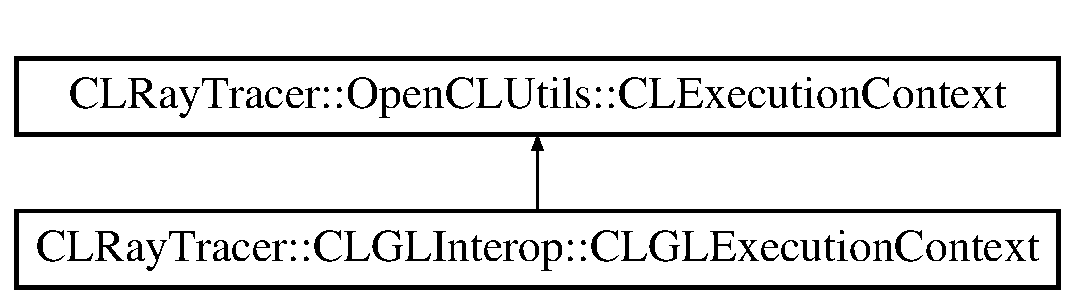
\includegraphics[height=2.000000cm]{class_c_l_ray_tracer_1_1_c_l_g_l_interop_1_1_c_l_g_l_execution_context}
\end{center}
\end{figure}
\subsection*{Public Member Functions}
\begin{DoxyCompactItemize}
\item 
\hyperlink{class_c_l_ray_tracer_1_1_c_l_g_l_interop_1_1_c_l_g_l_execution_context_af723c8184d47e2a41f72cb2690824121}{C\+L\+G\+L\+Execution\+Context} (const \hyperlink{class_c_l_ray_tracer_1_1_open_c_l_utils_1_1_c_l_device}{Open\+C\+L\+Utils\+::\+C\+L\+Device} \&device, const cl\+\_\+context\+\_\+properties $\ast$\+\_\+context\+Properties=N\+U\+LL)
\item 
virtual \hyperlink{class_c_l_ray_tracer_1_1_c_l_g_l_interop_1_1_c_l_g_l_execution_context_a177101743f53442a579e33864368458a}{$\sim$\+C\+L\+G\+L\+Execution\+Context} ()
\item 
\hyperlink{_errata_8h_a389396702f1aff6e71eb21328b0775c1}{Common\+::\+Result} \hyperlink{class_c_l_ray_tracer_1_1_c_l_g_l_interop_1_1_c_l_g_l_execution_context_a9168c916f733e28118b0f19acb97573e}{create\+C\+L\+G\+L\+Buffer} (void $\ast$data, size\+\_\+t size, boost\+::shared\+\_\+ptr$<$ \hyperlink{class_c_l_ray_tracer_1_1_c_l_g_l_interop_1_1_c_l_g_l_memory_buffer}{C\+L\+G\+L\+Memory\+Buffer} $>$ \&out\+\_\+buffer, \hyperlink{class_c_l_ray_tracer_1_1_common_1_1_errata}{Common\+::\+Errata} \&err) const 
\item 
\hyperlink{_errata_8h_a389396702f1aff6e71eb21328b0775c1}{Common\+::\+Result} \hyperlink{class_c_l_ray_tracer_1_1_c_l_g_l_interop_1_1_c_l_g_l_execution_context_ada8a14d2f88ff743e65242a39536cf5e}{create\+C\+L\+G\+L\+Buffer} (size\+\_\+t size, boost\+::shared\+\_\+ptr$<$ \hyperlink{class_c_l_ray_tracer_1_1_c_l_g_l_interop_1_1_c_l_g_l_memory_buffer}{C\+L\+G\+L\+Memory\+Buffer} $>$ \&out\+\_\+buffer, \hyperlink{class_c_l_ray_tracer_1_1_common_1_1_errata}{Common\+::\+Errata} \&err) const 
\item 
\hyperlink{_errata_8h_a389396702f1aff6e71eb21328b0775c1}{Common\+::\+Result} \hyperlink{class_c_l_ray_tracer_1_1_c_l_g_l_interop_1_1_c_l_g_l_execution_context_a6aa0a4371ced825dbf1ad15bc731c344}{enqueue\+Acquire\+G\+L\+Object} (std\+::vector$<$ cl\+\_\+mem $>$ objects, \hyperlink{class_c_l_ray_tracer_1_1_open_c_l_utils_1_1_c_l_event}{Open\+C\+L\+Utils\+::\+C\+L\+Event} \&evt, \hyperlink{class_c_l_ray_tracer_1_1_common_1_1_errata}{Common\+::\+Errata} \&err) const 
\item 
\hyperlink{_errata_8h_a389396702f1aff6e71eb21328b0775c1}{Common\+::\+Result} \hyperlink{class_c_l_ray_tracer_1_1_c_l_g_l_interop_1_1_c_l_g_l_execution_context_ab10596b7db9da5e60e095a6d5ed91ce4}{enqueue\+Acquire\+G\+L\+Object} (std\+::vector$<$ cl\+\_\+mem $>$ objects, \hyperlink{class_c_l_ray_tracer_1_1_common_1_1_errata}{Common\+::\+Errata} \&err) const 
\item 
\hyperlink{_errata_8h_a389396702f1aff6e71eb21328b0775c1}{Common\+::\+Result} \hyperlink{class_c_l_ray_tracer_1_1_c_l_g_l_interop_1_1_c_l_g_l_execution_context_a0af4a2fceda62535297fb5b70033826b}{enqueue\+Release\+G\+L\+Object} (std\+::vector$<$ cl\+\_\+mem $>$ objects, \hyperlink{class_c_l_ray_tracer_1_1_open_c_l_utils_1_1_c_l_event}{Open\+C\+L\+Utils\+::\+C\+L\+Event} \&evt, \hyperlink{class_c_l_ray_tracer_1_1_common_1_1_errata}{Common\+::\+Errata} \&err) const 
\item 
\hyperlink{_errata_8h_a389396702f1aff6e71eb21328b0775c1}{Common\+::\+Result} \hyperlink{class_c_l_ray_tracer_1_1_c_l_g_l_interop_1_1_c_l_g_l_execution_context_ab127d4b7e70b2e5b8431e6e615003597}{enqueue\+Release\+G\+L\+Object} (std\+::vector$<$ cl\+\_\+mem $>$ objects, \hyperlink{class_c_l_ray_tracer_1_1_common_1_1_errata}{Common\+::\+Errata} \&err) const 
\end{DoxyCompactItemize}
\subsection*{Additional Inherited Members}


\subsection{Detailed Description}
class \hyperlink{class_c_l_ray_tracer_1_1_c_l_g_l_interop_1_1_c_l_g_l_execution_context}{C\+L\+G\+L\+Execution\+Context} Extends C\+L\+Execution\+Context with Open\+C\+L/\+Open\+GL interop functions. 

\subsection{Constructor \& Destructor Documentation}
\index{C\+L\+Ray\+Tracer\+::\+C\+L\+G\+L\+Interop\+::\+C\+L\+G\+L\+Execution\+Context@{C\+L\+Ray\+Tracer\+::\+C\+L\+G\+L\+Interop\+::\+C\+L\+G\+L\+Execution\+Context}!C\+L\+G\+L\+Execution\+Context@{C\+L\+G\+L\+Execution\+Context}}
\index{C\+L\+G\+L\+Execution\+Context@{C\+L\+G\+L\+Execution\+Context}!C\+L\+Ray\+Tracer\+::\+C\+L\+G\+L\+Interop\+::\+C\+L\+G\+L\+Execution\+Context@{C\+L\+Ray\+Tracer\+::\+C\+L\+G\+L\+Interop\+::\+C\+L\+G\+L\+Execution\+Context}}
\subsubsection[{\texorpdfstring{C\+L\+G\+L\+Execution\+Context(const Open\+C\+L\+Utils\+::\+C\+L\+Device \&device, const cl\+\_\+context\+\_\+properties $\ast$\+\_\+context\+Properties=\+N\+U\+L\+L)}{CLGLExecutionContext(const OpenCLUtils::CLDevice &device, const cl_context_properties *_contextProperties=NULL)}}]{\setlength{\rightskip}{0pt plus 5cm}C\+L\+Ray\+Tracer\+::\+C\+L\+G\+L\+Interop\+::\+C\+L\+G\+L\+Execution\+Context\+::\+C\+L\+G\+L\+Execution\+Context (
\begin{DoxyParamCaption}
\item[{const {\bf Open\+C\+L\+Utils\+::\+C\+L\+Device} \&}]{device, }
\item[{const cl\+\_\+context\+\_\+properties $\ast$}]{\+\_\+context\+Properties = {\ttfamily NULL}}
\end{DoxyParamCaption}
)\hspace{0.3cm}{\ttfamily [inline]}}\hypertarget{class_c_l_ray_tracer_1_1_c_l_g_l_interop_1_1_c_l_g_l_execution_context_af723c8184d47e2a41f72cb2690824121}{}\label{class_c_l_ray_tracer_1_1_c_l_g_l_interop_1_1_c_l_g_l_execution_context_af723c8184d47e2a41f72cb2690824121}
Constructor 
\begin{DoxyParams}{Parameters}
{\em device} & Object that encapsulate the Open\+CL device in use \\
\hline
{\em context\+Properties\mbox{[}optional\mbox{]}} & The properties of context to be created \\
\hline
\end{DoxyParams}
\begin{DoxySeeAlso}{See also}
class C\+L\+Device 

cl\+\_\+context\+\_\+properties in Open\+CL specification 
\end{DoxySeeAlso}
\index{C\+L\+Ray\+Tracer\+::\+C\+L\+G\+L\+Interop\+::\+C\+L\+G\+L\+Execution\+Context@{C\+L\+Ray\+Tracer\+::\+C\+L\+G\+L\+Interop\+::\+C\+L\+G\+L\+Execution\+Context}!````~C\+L\+G\+L\+Execution\+Context@{$\sim$\+C\+L\+G\+L\+Execution\+Context}}
\index{````~C\+L\+G\+L\+Execution\+Context@{$\sim$\+C\+L\+G\+L\+Execution\+Context}!C\+L\+Ray\+Tracer\+::\+C\+L\+G\+L\+Interop\+::\+C\+L\+G\+L\+Execution\+Context@{C\+L\+Ray\+Tracer\+::\+C\+L\+G\+L\+Interop\+::\+C\+L\+G\+L\+Execution\+Context}}
\subsubsection[{\texorpdfstring{$\sim$\+C\+L\+G\+L\+Execution\+Context()}{~CLGLExecutionContext()}}]{\setlength{\rightskip}{0pt plus 5cm}virtual C\+L\+Ray\+Tracer\+::\+C\+L\+G\+L\+Interop\+::\+C\+L\+G\+L\+Execution\+Context\+::$\sim$\+C\+L\+G\+L\+Execution\+Context (
\begin{DoxyParamCaption}
{}
\end{DoxyParamCaption}
)\hspace{0.3cm}{\ttfamily [virtual]}}\hypertarget{class_c_l_ray_tracer_1_1_c_l_g_l_interop_1_1_c_l_g_l_execution_context_a177101743f53442a579e33864368458a}{}\label{class_c_l_ray_tracer_1_1_c_l_g_l_interop_1_1_c_l_g_l_execution_context_a177101743f53442a579e33864368458a}
Destructor 

\subsection{Member Function Documentation}
\index{C\+L\+Ray\+Tracer\+::\+C\+L\+G\+L\+Interop\+::\+C\+L\+G\+L\+Execution\+Context@{C\+L\+Ray\+Tracer\+::\+C\+L\+G\+L\+Interop\+::\+C\+L\+G\+L\+Execution\+Context}!create\+C\+L\+G\+L\+Buffer@{create\+C\+L\+G\+L\+Buffer}}
\index{create\+C\+L\+G\+L\+Buffer@{create\+C\+L\+G\+L\+Buffer}!C\+L\+Ray\+Tracer\+::\+C\+L\+G\+L\+Interop\+::\+C\+L\+G\+L\+Execution\+Context@{C\+L\+Ray\+Tracer\+::\+C\+L\+G\+L\+Interop\+::\+C\+L\+G\+L\+Execution\+Context}}
\subsubsection[{\texorpdfstring{create\+C\+L\+G\+L\+Buffer(void $\ast$data, size\+\_\+t size, boost\+::shared\+\_\+ptr$<$ C\+L\+G\+L\+Memory\+Buffer $>$ \&out\+\_\+buffer, Common\+::\+Errata \&err) const }{createCLGLBuffer(void *data, size_t size, boost::shared_ptr< CLGLMemoryBuffer > &out_buffer, Common::Errata &err) const }}]{\setlength{\rightskip}{0pt plus 5cm}{\bf Common\+::\+Result} C\+L\+Ray\+Tracer\+::\+C\+L\+G\+L\+Interop\+::\+C\+L\+G\+L\+Execution\+Context\+::create\+C\+L\+G\+L\+Buffer (
\begin{DoxyParamCaption}
\item[{void $\ast$}]{data, }
\item[{size\+\_\+t}]{size, }
\item[{boost\+::shared\+\_\+ptr$<$ {\bf C\+L\+G\+L\+Memory\+Buffer} $>$ \&}]{out\+\_\+buffer, }
\item[{{\bf Common\+::\+Errata} \&}]{err}
\end{DoxyParamCaption}
) const}\hypertarget{class_c_l_ray_tracer_1_1_c_l_g_l_interop_1_1_c_l_g_l_execution_context_a9168c916f733e28118b0f19acb97573e}{}\label{class_c_l_ray_tracer_1_1_c_l_g_l_interop_1_1_c_l_g_l_execution_context_a9168c916f733e28118b0f19acb97573e}
Create Open\+C\+L/\+Open\+GL memory object for inter-\/operation 
\begin{DoxyParams}[1]{Parameters}
 & {\em data} & The host data that should be copied to the Open\+G\+L/\+Open\+CL buffer on creation \\
\hline
 & {\em size} & Desired size of the buffer \\
\hline
\mbox{\tt out}  & {\em } & \\
\hline
\end{DoxyParams}
\index{C\+L\+Ray\+Tracer\+::\+C\+L\+G\+L\+Interop\+::\+C\+L\+G\+L\+Execution\+Context@{C\+L\+Ray\+Tracer\+::\+C\+L\+G\+L\+Interop\+::\+C\+L\+G\+L\+Execution\+Context}!create\+C\+L\+G\+L\+Buffer@{create\+C\+L\+G\+L\+Buffer}}
\index{create\+C\+L\+G\+L\+Buffer@{create\+C\+L\+G\+L\+Buffer}!C\+L\+Ray\+Tracer\+::\+C\+L\+G\+L\+Interop\+::\+C\+L\+G\+L\+Execution\+Context@{C\+L\+Ray\+Tracer\+::\+C\+L\+G\+L\+Interop\+::\+C\+L\+G\+L\+Execution\+Context}}
\subsubsection[{\texorpdfstring{create\+C\+L\+G\+L\+Buffer(size\+\_\+t size, boost\+::shared\+\_\+ptr$<$ C\+L\+G\+L\+Memory\+Buffer $>$ \&out\+\_\+buffer, Common\+::\+Errata \&err) const }{createCLGLBuffer(size_t size, boost::shared_ptr< CLGLMemoryBuffer > &out_buffer, Common::Errata &err) const }}]{\setlength{\rightskip}{0pt plus 5cm}{\bf Common\+::\+Result} C\+L\+Ray\+Tracer\+::\+C\+L\+G\+L\+Interop\+::\+C\+L\+G\+L\+Execution\+Context\+::create\+C\+L\+G\+L\+Buffer (
\begin{DoxyParamCaption}
\item[{size\+\_\+t}]{size, }
\item[{boost\+::shared\+\_\+ptr$<$ {\bf C\+L\+G\+L\+Memory\+Buffer} $>$ \&}]{out\+\_\+buffer, }
\item[{{\bf Common\+::\+Errata} \&}]{err}
\end{DoxyParamCaption}
) const}\hypertarget{class_c_l_ray_tracer_1_1_c_l_g_l_interop_1_1_c_l_g_l_execution_context_ada8a14d2f88ff743e65242a39536cf5e}{}\label{class_c_l_ray_tracer_1_1_c_l_g_l_interop_1_1_c_l_g_l_execution_context_ada8a14d2f88ff743e65242a39536cf5e}
Create Open\+C\+L/\+Open\+GL memory object for inter-\/operation 
\begin{DoxyParams}[1]{Parameters}
 & {\em size} & Desired size of the buffer \\
\hline
\mbox{\tt out}  & {\em } & \\
\hline
\end{DoxyParams}
\index{C\+L\+Ray\+Tracer\+::\+C\+L\+G\+L\+Interop\+::\+C\+L\+G\+L\+Execution\+Context@{C\+L\+Ray\+Tracer\+::\+C\+L\+G\+L\+Interop\+::\+C\+L\+G\+L\+Execution\+Context}!enqueue\+Acquire\+G\+L\+Object@{enqueue\+Acquire\+G\+L\+Object}}
\index{enqueue\+Acquire\+G\+L\+Object@{enqueue\+Acquire\+G\+L\+Object}!C\+L\+Ray\+Tracer\+::\+C\+L\+G\+L\+Interop\+::\+C\+L\+G\+L\+Execution\+Context@{C\+L\+Ray\+Tracer\+::\+C\+L\+G\+L\+Interop\+::\+C\+L\+G\+L\+Execution\+Context}}
\subsubsection[{\texorpdfstring{enqueue\+Acquire\+G\+L\+Object(std\+::vector$<$ cl\+\_\+mem $>$ objects, Open\+C\+L\+Utils\+::\+C\+L\+Event \&evt, Common\+::\+Errata \&err) const }{enqueueAcquireGLObject(std::vector< cl_mem > objects, OpenCLUtils::CLEvent &evt, Common::Errata &err) const }}]{\setlength{\rightskip}{0pt plus 5cm}{\bf Common\+::\+Result} C\+L\+Ray\+Tracer\+::\+C\+L\+G\+L\+Interop\+::\+C\+L\+G\+L\+Execution\+Context\+::enqueue\+Acquire\+G\+L\+Object (
\begin{DoxyParamCaption}
\item[{std\+::vector$<$ cl\+\_\+mem $>$}]{objects, }
\item[{{\bf Open\+C\+L\+Utils\+::\+C\+L\+Event} \&}]{evt, }
\item[{{\bf Common\+::\+Errata} \&}]{err}
\end{DoxyParamCaption}
) const}\hypertarget{class_c_l_ray_tracer_1_1_c_l_g_l_interop_1_1_c_l_g_l_execution_context_a6aa0a4371ced825dbf1ad15bc731c344}{}\label{class_c_l_ray_tracer_1_1_c_l_g_l_interop_1_1_c_l_g_l_execution_context_a6aa0a4371ced825dbf1ad15bc731c344}
Acquire memory object for use with Open\+CL memory operations 
\begin{DoxyParams}{Parameters}
{\em object} & Memory objects list \\
\hline
{\em evt} & Events to wait for, before proceeding to this operation \\
\hline
{\em err} & Error info \\
\hline
\end{DoxyParams}
\begin{DoxyReturn}{Returns}
Result of the operation\+: Success or failure 
\end{DoxyReturn}
\index{C\+L\+Ray\+Tracer\+::\+C\+L\+G\+L\+Interop\+::\+C\+L\+G\+L\+Execution\+Context@{C\+L\+Ray\+Tracer\+::\+C\+L\+G\+L\+Interop\+::\+C\+L\+G\+L\+Execution\+Context}!enqueue\+Acquire\+G\+L\+Object@{enqueue\+Acquire\+G\+L\+Object}}
\index{enqueue\+Acquire\+G\+L\+Object@{enqueue\+Acquire\+G\+L\+Object}!C\+L\+Ray\+Tracer\+::\+C\+L\+G\+L\+Interop\+::\+C\+L\+G\+L\+Execution\+Context@{C\+L\+Ray\+Tracer\+::\+C\+L\+G\+L\+Interop\+::\+C\+L\+G\+L\+Execution\+Context}}
\subsubsection[{\texorpdfstring{enqueue\+Acquire\+G\+L\+Object(std\+::vector$<$ cl\+\_\+mem $>$ objects, Common\+::\+Errata \&err) const }{enqueueAcquireGLObject(std::vector< cl_mem > objects, Common::Errata &err) const }}]{\setlength{\rightskip}{0pt plus 5cm}{\bf Common\+::\+Result} C\+L\+Ray\+Tracer\+::\+C\+L\+G\+L\+Interop\+::\+C\+L\+G\+L\+Execution\+Context\+::enqueue\+Acquire\+G\+L\+Object (
\begin{DoxyParamCaption}
\item[{std\+::vector$<$ cl\+\_\+mem $>$}]{objects, }
\item[{{\bf Common\+::\+Errata} \&}]{err}
\end{DoxyParamCaption}
) const}\hypertarget{class_c_l_ray_tracer_1_1_c_l_g_l_interop_1_1_c_l_g_l_execution_context_ab10596b7db9da5e60e095a6d5ed91ce4}{}\label{class_c_l_ray_tracer_1_1_c_l_g_l_interop_1_1_c_l_g_l_execution_context_ab10596b7db9da5e60e095a6d5ed91ce4}
Acquire memory object for use with Open\+CL memory operations 
\begin{DoxyParams}{Parameters}
{\em object} & Memory objects list \\
\hline
{\em err} & Error info \\
\hline
\end{DoxyParams}
\begin{DoxyReturn}{Returns}
Result of the operation\+: Success or failure 
\end{DoxyReturn}
\index{C\+L\+Ray\+Tracer\+::\+C\+L\+G\+L\+Interop\+::\+C\+L\+G\+L\+Execution\+Context@{C\+L\+Ray\+Tracer\+::\+C\+L\+G\+L\+Interop\+::\+C\+L\+G\+L\+Execution\+Context}!enqueue\+Release\+G\+L\+Object@{enqueue\+Release\+G\+L\+Object}}
\index{enqueue\+Release\+G\+L\+Object@{enqueue\+Release\+G\+L\+Object}!C\+L\+Ray\+Tracer\+::\+C\+L\+G\+L\+Interop\+::\+C\+L\+G\+L\+Execution\+Context@{C\+L\+Ray\+Tracer\+::\+C\+L\+G\+L\+Interop\+::\+C\+L\+G\+L\+Execution\+Context}}
\subsubsection[{\texorpdfstring{enqueue\+Release\+G\+L\+Object(std\+::vector$<$ cl\+\_\+mem $>$ objects, Open\+C\+L\+Utils\+::\+C\+L\+Event \&evt, Common\+::\+Errata \&err) const }{enqueueReleaseGLObject(std::vector< cl_mem > objects, OpenCLUtils::CLEvent &evt, Common::Errata &err) const }}]{\setlength{\rightskip}{0pt plus 5cm}{\bf Common\+::\+Result} C\+L\+Ray\+Tracer\+::\+C\+L\+G\+L\+Interop\+::\+C\+L\+G\+L\+Execution\+Context\+::enqueue\+Release\+G\+L\+Object (
\begin{DoxyParamCaption}
\item[{std\+::vector$<$ cl\+\_\+mem $>$}]{objects, }
\item[{{\bf Open\+C\+L\+Utils\+::\+C\+L\+Event} \&}]{evt, }
\item[{{\bf Common\+::\+Errata} \&}]{err}
\end{DoxyParamCaption}
) const}\hypertarget{class_c_l_ray_tracer_1_1_c_l_g_l_interop_1_1_c_l_g_l_execution_context_a0af4a2fceda62535297fb5b70033826b}{}\label{class_c_l_ray_tracer_1_1_c_l_g_l_interop_1_1_c_l_g_l_execution_context_a0af4a2fceda62535297fb5b70033826b}
Release memory object for use by Open\+GL 
\begin{DoxyParams}{Parameters}
{\em object} & Memory objects list \\
\hline
{\em evt} & Events to wait for, before proceeding to this operation \\
\hline
{\em err} & Error info \\
\hline
\end{DoxyParams}
\begin{DoxyReturn}{Returns}
Result of the operation\+: Success or failure 
\end{DoxyReturn}
\index{C\+L\+Ray\+Tracer\+::\+C\+L\+G\+L\+Interop\+::\+C\+L\+G\+L\+Execution\+Context@{C\+L\+Ray\+Tracer\+::\+C\+L\+G\+L\+Interop\+::\+C\+L\+G\+L\+Execution\+Context}!enqueue\+Release\+G\+L\+Object@{enqueue\+Release\+G\+L\+Object}}
\index{enqueue\+Release\+G\+L\+Object@{enqueue\+Release\+G\+L\+Object}!C\+L\+Ray\+Tracer\+::\+C\+L\+G\+L\+Interop\+::\+C\+L\+G\+L\+Execution\+Context@{C\+L\+Ray\+Tracer\+::\+C\+L\+G\+L\+Interop\+::\+C\+L\+G\+L\+Execution\+Context}}
\subsubsection[{\texorpdfstring{enqueue\+Release\+G\+L\+Object(std\+::vector$<$ cl\+\_\+mem $>$ objects, Common\+::\+Errata \&err) const }{enqueueReleaseGLObject(std::vector< cl_mem > objects, Common::Errata &err) const }}]{\setlength{\rightskip}{0pt plus 5cm}{\bf Common\+::\+Result} C\+L\+Ray\+Tracer\+::\+C\+L\+G\+L\+Interop\+::\+C\+L\+G\+L\+Execution\+Context\+::enqueue\+Release\+G\+L\+Object (
\begin{DoxyParamCaption}
\item[{std\+::vector$<$ cl\+\_\+mem $>$}]{objects, }
\item[{{\bf Common\+::\+Errata} \&}]{err}
\end{DoxyParamCaption}
) const}\hypertarget{class_c_l_ray_tracer_1_1_c_l_g_l_interop_1_1_c_l_g_l_execution_context_ab127d4b7e70b2e5b8431e6e615003597}{}\label{class_c_l_ray_tracer_1_1_c_l_g_l_interop_1_1_c_l_g_l_execution_context_ab127d4b7e70b2e5b8431e6e615003597}
Release memory object for use by Open\+GL 
\begin{DoxyParams}{Parameters}
{\em object} & Memory objects list \\
\hline
{\em err} & Error info \\
\hline
\end{DoxyParams}
\begin{DoxyReturn}{Returns}
Result of the operation\+: Success or failure 
\end{DoxyReturn}


The documentation for this class was generated from the following file\+:\begin{DoxyCompactItemize}
\item 
Include/\+Open\+C\+L\+Utils/\hyperlink{_c_l_g_l_execution_context_8h}{C\+L\+G\+L\+Execution\+Context.\+h}\end{DoxyCompactItemize}

\hypertarget{class_c_l_ray_tracer_1_1_c_l_g_l_interop_1_1_c_l_g_l_interop_context}{}\section{C\+L\+Ray\+Tracer\+:\+:C\+L\+G\+L\+Interop\+:\+:C\+L\+G\+L\+Interop\+Context Class Reference}
\label{class_c_l_ray_tracer_1_1_c_l_g_l_interop_1_1_c_l_g_l_interop_context}\index{C\+L\+Ray\+Tracer\+::\+C\+L\+G\+L\+Interop\+::\+C\+L\+G\+L\+Interop\+Context@{C\+L\+Ray\+Tracer\+::\+C\+L\+G\+L\+Interop\+::\+C\+L\+G\+L\+Interop\+Context}}


{\ttfamily \#include $<$C\+L\+G\+L\+Interop\+Context.\+h$>$}

\subsection*{Public Member Functions}
\begin{DoxyCompactItemize}
\item 
\hyperlink{_errata_8h_a389396702f1aff6e71eb21328b0775c1}{Common\+::\+Result} \hyperlink{class_c_l_ray_tracer_1_1_c_l_g_l_interop_1_1_c_l_g_l_interop_context_a4f391524b83a921d711403ee443a11a7}{initialize} (const \hyperlink{class_c_l_ray_tracer_1_1_open_c_l_utils_1_1_c_l_platform}{Open\+C\+L\+Utils\+::\+C\+L\+Platform} \&platform, \hyperlink{class_c_l_ray_tracer_1_1_common_1_1_errata}{Common\+::\+Errata} \&err)
\item 
\hyperlink{_errata_8h_a389396702f1aff6e71eb21328b0775c1}{Common\+::\+Result} \hyperlink{class_c_l_ray_tracer_1_1_c_l_g_l_interop_1_1_c_l_g_l_interop_context_a1e08d7458413f12c8a7547813c8b1b82}{initialize} (const \hyperlink{class_c_l_ray_tracer_1_1_open_c_l_utils_1_1_c_l_interface}{Open\+C\+L\+Utils\+::\+C\+L\+Interface} \&cl\+Interface, \hyperlink{class_c_l_ray_tracer_1_1_common_1_1_errata}{Common\+::\+Errata} \&err)
\item 
const \hyperlink{class_c_l_ray_tracer_1_1_c_l_g_l_interop_1_1_c_l_g_l_execution_context}{C\+L\+G\+L\+Execution\+Context} $\ast$ \hyperlink{class_c_l_ray_tracer_1_1_c_l_g_l_interop_1_1_c_l_g_l_interop_context_a025373c5027d96fa8024c2fc3e1a7eea}{get\+Execution\+Context} () const 
\item 
const \hyperlink{class_c_l_ray_tracer_1_1_open_c_l_utils_1_1_c_l_platform}{Open\+C\+L\+Utils\+::\+C\+L\+Platform} $\ast$ \hyperlink{class_c_l_ray_tracer_1_1_c_l_g_l_interop_1_1_c_l_g_l_interop_context_a978b5f6a69cfbc54991c1b71db66e6b3}{get\+Interop\+Platform} () const 
\item 
const \hyperlink{class_c_l_ray_tracer_1_1_open_c_l_utils_1_1_c_l_device}{Open\+C\+L\+Utils\+::\+C\+L\+Device} $\ast$ \hyperlink{class_c_l_ray_tracer_1_1_c_l_g_l_interop_1_1_c_l_g_l_interop_context_aa62034aeda5335d2fc1933186457d408}{get\+Interop\+Device} () const 
\item 
\hyperlink{class_c_l_ray_tracer_1_1_c_l_g_l_interop_1_1_c_l_g_l_interop_context_a836720a22d2c13a846d18cbde819f5e9}{C\+L\+G\+L\+Interop\+Context} ()
\item 
virtual \hyperlink{class_c_l_ray_tracer_1_1_c_l_g_l_interop_1_1_c_l_g_l_interop_context_a2be07d7835bbad957b12145d49b8afcc}{$\sim$\+C\+L\+G\+L\+Interop\+Context} ()
\end{DoxyCompactItemize}


\subsection{Detailed Description}
class \hyperlink{class_c_l_ray_tracer_1_1_c_l_g_l_interop_1_1_c_l_g_l_interop_context}{C\+L\+G\+L\+Interop\+Context} exposes functionality for Open\+G\+L/\+Open\+CL interop 

\subsection{Constructor \& Destructor Documentation}
\index{C\+L\+Ray\+Tracer\+::\+C\+L\+G\+L\+Interop\+::\+C\+L\+G\+L\+Interop\+Context@{C\+L\+Ray\+Tracer\+::\+C\+L\+G\+L\+Interop\+::\+C\+L\+G\+L\+Interop\+Context}!C\+L\+G\+L\+Interop\+Context@{C\+L\+G\+L\+Interop\+Context}}
\index{C\+L\+G\+L\+Interop\+Context@{C\+L\+G\+L\+Interop\+Context}!C\+L\+Ray\+Tracer\+::\+C\+L\+G\+L\+Interop\+::\+C\+L\+G\+L\+Interop\+Context@{C\+L\+Ray\+Tracer\+::\+C\+L\+G\+L\+Interop\+::\+C\+L\+G\+L\+Interop\+Context}}
\subsubsection[{\texorpdfstring{C\+L\+G\+L\+Interop\+Context()}{CLGLInteropContext()}}]{\setlength{\rightskip}{0pt plus 5cm}C\+L\+Ray\+Tracer\+::\+C\+L\+G\+L\+Interop\+::\+C\+L\+G\+L\+Interop\+Context\+::\+C\+L\+G\+L\+Interop\+Context (
\begin{DoxyParamCaption}
{}
\end{DoxyParamCaption}
)}\hypertarget{class_c_l_ray_tracer_1_1_c_l_g_l_interop_1_1_c_l_g_l_interop_context_a836720a22d2c13a846d18cbde819f5e9}{}\label{class_c_l_ray_tracer_1_1_c_l_g_l_interop_1_1_c_l_g_l_interop_context_a836720a22d2c13a846d18cbde819f5e9}
Constructor \index{C\+L\+Ray\+Tracer\+::\+C\+L\+G\+L\+Interop\+::\+C\+L\+G\+L\+Interop\+Context@{C\+L\+Ray\+Tracer\+::\+C\+L\+G\+L\+Interop\+::\+C\+L\+G\+L\+Interop\+Context}!````~C\+L\+G\+L\+Interop\+Context@{$\sim$\+C\+L\+G\+L\+Interop\+Context}}
\index{````~C\+L\+G\+L\+Interop\+Context@{$\sim$\+C\+L\+G\+L\+Interop\+Context}!C\+L\+Ray\+Tracer\+::\+C\+L\+G\+L\+Interop\+::\+C\+L\+G\+L\+Interop\+Context@{C\+L\+Ray\+Tracer\+::\+C\+L\+G\+L\+Interop\+::\+C\+L\+G\+L\+Interop\+Context}}
\subsubsection[{\texorpdfstring{$\sim$\+C\+L\+G\+L\+Interop\+Context()}{~CLGLInteropContext()}}]{\setlength{\rightskip}{0pt plus 5cm}virtual C\+L\+Ray\+Tracer\+::\+C\+L\+G\+L\+Interop\+::\+C\+L\+G\+L\+Interop\+Context\+::$\sim$\+C\+L\+G\+L\+Interop\+Context (
\begin{DoxyParamCaption}
{}
\end{DoxyParamCaption}
)\hspace{0.3cm}{\ttfamily [virtual]}}\hypertarget{class_c_l_ray_tracer_1_1_c_l_g_l_interop_1_1_c_l_g_l_interop_context_a2be07d7835bbad957b12145d49b8afcc}{}\label{class_c_l_ray_tracer_1_1_c_l_g_l_interop_1_1_c_l_g_l_interop_context_a2be07d7835bbad957b12145d49b8afcc}
Destructor 

\subsection{Member Function Documentation}
\index{C\+L\+Ray\+Tracer\+::\+C\+L\+G\+L\+Interop\+::\+C\+L\+G\+L\+Interop\+Context@{C\+L\+Ray\+Tracer\+::\+C\+L\+G\+L\+Interop\+::\+C\+L\+G\+L\+Interop\+Context}!get\+Execution\+Context@{get\+Execution\+Context}}
\index{get\+Execution\+Context@{get\+Execution\+Context}!C\+L\+Ray\+Tracer\+::\+C\+L\+G\+L\+Interop\+::\+C\+L\+G\+L\+Interop\+Context@{C\+L\+Ray\+Tracer\+::\+C\+L\+G\+L\+Interop\+::\+C\+L\+G\+L\+Interop\+Context}}
\subsubsection[{\texorpdfstring{get\+Execution\+Context() const }{getExecutionContext() const }}]{\setlength{\rightskip}{0pt plus 5cm}const {\bf C\+L\+G\+L\+Execution\+Context}$\ast$ C\+L\+Ray\+Tracer\+::\+C\+L\+G\+L\+Interop\+::\+C\+L\+G\+L\+Interop\+Context\+::get\+Execution\+Context (
\begin{DoxyParamCaption}
{}
\end{DoxyParamCaption}
) const\hspace{0.3cm}{\ttfamily [inline]}}\hypertarget{class_c_l_ray_tracer_1_1_c_l_g_l_interop_1_1_c_l_g_l_interop_context_a025373c5027d96fa8024c2fc3e1a7eea}{}\label{class_c_l_ray_tracer_1_1_c_l_g_l_interop_1_1_c_l_g_l_interop_context_a025373c5027d96fa8024c2fc3e1a7eea}
Retrieves the associated Execution Context object \begin{DoxyReturn}{Returns}
The associated Execution Context object 
\end{DoxyReturn}
\index{C\+L\+Ray\+Tracer\+::\+C\+L\+G\+L\+Interop\+::\+C\+L\+G\+L\+Interop\+Context@{C\+L\+Ray\+Tracer\+::\+C\+L\+G\+L\+Interop\+::\+C\+L\+G\+L\+Interop\+Context}!get\+Interop\+Device@{get\+Interop\+Device}}
\index{get\+Interop\+Device@{get\+Interop\+Device}!C\+L\+Ray\+Tracer\+::\+C\+L\+G\+L\+Interop\+::\+C\+L\+G\+L\+Interop\+Context@{C\+L\+Ray\+Tracer\+::\+C\+L\+G\+L\+Interop\+::\+C\+L\+G\+L\+Interop\+Context}}
\subsubsection[{\texorpdfstring{get\+Interop\+Device() const }{getInteropDevice() const }}]{\setlength{\rightskip}{0pt plus 5cm}const {\bf Open\+C\+L\+Utils\+::\+C\+L\+Device}$\ast$ C\+L\+Ray\+Tracer\+::\+C\+L\+G\+L\+Interop\+::\+C\+L\+G\+L\+Interop\+Context\+::get\+Interop\+Device (
\begin{DoxyParamCaption}
{}
\end{DoxyParamCaption}
) const\hspace{0.3cm}{\ttfamily [inline]}}\hypertarget{class_c_l_ray_tracer_1_1_c_l_g_l_interop_1_1_c_l_g_l_interop_context_aa62034aeda5335d2fc1933186457d408}{}\label{class_c_l_ray_tracer_1_1_c_l_g_l_interop_1_1_c_l_g_l_interop_context_aa62034aeda5335d2fc1933186457d408}
Retrieves the associated Open\+CL device \begin{DoxyReturn}{Returns}
The associated Open\+CL device 
\end{DoxyReturn}
\index{C\+L\+Ray\+Tracer\+::\+C\+L\+G\+L\+Interop\+::\+C\+L\+G\+L\+Interop\+Context@{C\+L\+Ray\+Tracer\+::\+C\+L\+G\+L\+Interop\+::\+C\+L\+G\+L\+Interop\+Context}!get\+Interop\+Platform@{get\+Interop\+Platform}}
\index{get\+Interop\+Platform@{get\+Interop\+Platform}!C\+L\+Ray\+Tracer\+::\+C\+L\+G\+L\+Interop\+::\+C\+L\+G\+L\+Interop\+Context@{C\+L\+Ray\+Tracer\+::\+C\+L\+G\+L\+Interop\+::\+C\+L\+G\+L\+Interop\+Context}}
\subsubsection[{\texorpdfstring{get\+Interop\+Platform() const }{getInteropPlatform() const }}]{\setlength{\rightskip}{0pt plus 5cm}const {\bf Open\+C\+L\+Utils\+::\+C\+L\+Platform}$\ast$ C\+L\+Ray\+Tracer\+::\+C\+L\+G\+L\+Interop\+::\+C\+L\+G\+L\+Interop\+Context\+::get\+Interop\+Platform (
\begin{DoxyParamCaption}
{}
\end{DoxyParamCaption}
) const\hspace{0.3cm}{\ttfamily [inline]}}\hypertarget{class_c_l_ray_tracer_1_1_c_l_g_l_interop_1_1_c_l_g_l_interop_context_a978b5f6a69cfbc54991c1b71db66e6b3}{}\label{class_c_l_ray_tracer_1_1_c_l_g_l_interop_1_1_c_l_g_l_interop_context_a978b5f6a69cfbc54991c1b71db66e6b3}
Retrieves the associated Open\+CL platform \begin{DoxyReturn}{Returns}
The associated Open\+CL platform 
\end{DoxyReturn}
\index{C\+L\+Ray\+Tracer\+::\+C\+L\+G\+L\+Interop\+::\+C\+L\+G\+L\+Interop\+Context@{C\+L\+Ray\+Tracer\+::\+C\+L\+G\+L\+Interop\+::\+C\+L\+G\+L\+Interop\+Context}!initialize@{initialize}}
\index{initialize@{initialize}!C\+L\+Ray\+Tracer\+::\+C\+L\+G\+L\+Interop\+::\+C\+L\+G\+L\+Interop\+Context@{C\+L\+Ray\+Tracer\+::\+C\+L\+G\+L\+Interop\+::\+C\+L\+G\+L\+Interop\+Context}}
\subsubsection[{\texorpdfstring{initialize(const Open\+C\+L\+Utils\+::\+C\+L\+Platform \&platform, Common\+::\+Errata \&err)}{initialize(const OpenCLUtils::CLPlatform &platform, Common::Errata &err)}}]{\setlength{\rightskip}{0pt plus 5cm}{\bf Common\+::\+Result} C\+L\+Ray\+Tracer\+::\+C\+L\+G\+L\+Interop\+::\+C\+L\+G\+L\+Interop\+Context\+::initialize (
\begin{DoxyParamCaption}
\item[{const {\bf Open\+C\+L\+Utils\+::\+C\+L\+Platform} \&}]{platform, }
\item[{{\bf Common\+::\+Errata} \&}]{err}
\end{DoxyParamCaption}
)}\hypertarget{class_c_l_ray_tracer_1_1_c_l_g_l_interop_1_1_c_l_g_l_interop_context_a4f391524b83a921d711403ee443a11a7}{}\label{class_c_l_ray_tracer_1_1_c_l_g_l_interop_1_1_c_l_g_l_interop_context_a4f391524b83a921d711403ee443a11a7}
Initializes the object instance 
\begin{DoxyParams}{Parameters}
{\em platform} & Object that encapsulates the used Open\+CL platform \\
\hline
{\em err} & Error info \\
\hline
\end{DoxyParams}
\begin{DoxyReturn}{Returns}
Result of the operation\+: Success or failure 
\end{DoxyReturn}
\index{C\+L\+Ray\+Tracer\+::\+C\+L\+G\+L\+Interop\+::\+C\+L\+G\+L\+Interop\+Context@{C\+L\+Ray\+Tracer\+::\+C\+L\+G\+L\+Interop\+::\+C\+L\+G\+L\+Interop\+Context}!initialize@{initialize}}
\index{initialize@{initialize}!C\+L\+Ray\+Tracer\+::\+C\+L\+G\+L\+Interop\+::\+C\+L\+G\+L\+Interop\+Context@{C\+L\+Ray\+Tracer\+::\+C\+L\+G\+L\+Interop\+::\+C\+L\+G\+L\+Interop\+Context}}
\subsubsection[{\texorpdfstring{initialize(const Open\+C\+L\+Utils\+::\+C\+L\+Interface \&cl\+Interface, Common\+::\+Errata \&err)}{initialize(const OpenCLUtils::CLInterface &clInterface, Common::Errata &err)}}]{\setlength{\rightskip}{0pt plus 5cm}{\bf Common\+::\+Result} C\+L\+Ray\+Tracer\+::\+C\+L\+G\+L\+Interop\+::\+C\+L\+G\+L\+Interop\+Context\+::initialize (
\begin{DoxyParamCaption}
\item[{const {\bf Open\+C\+L\+Utils\+::\+C\+L\+Interface} \&}]{cl\+Interface, }
\item[{{\bf Common\+::\+Errata} \&}]{err}
\end{DoxyParamCaption}
)}\hypertarget{class_c_l_ray_tracer_1_1_c_l_g_l_interop_1_1_c_l_g_l_interop_context_a1e08d7458413f12c8a7547813c8b1b82}{}\label{class_c_l_ray_tracer_1_1_c_l_g_l_interop_1_1_c_l_g_l_interop_context_a1e08d7458413f12c8a7547813c8b1b82}
Initializes the object instance. Unlike the function that takes platform as parameter, this function automatically finds the first platform and device that support Open\+G\+L/\+Open\+CL interop and use that platform and device 
\begin{DoxyParams}{Parameters}
{\em C\+L\+Interface} & Object that encapsulates Open\+CL interface \\
\hline
{\em err} & Error info \\
\hline
\end{DoxyParams}
\begin{DoxyReturn}{Returns}
Result of the operation\+: Success or failure 
\end{DoxyReturn}


The documentation for this class was generated from the following file\+:\begin{DoxyCompactItemize}
\item 
Include/\+Open\+C\+L\+Utils/C\+L\+G\+L\+Interop\+Context.\+h\end{DoxyCompactItemize}

\hypertarget{class_c_l_ray_tracer_1_1_c_l_g_l_interop_1_1_c_l_g_l_memory_buffer}{}\section{C\+L\+Ray\+Tracer\+:\+:C\+L\+G\+L\+Interop\+:\+:C\+L\+G\+L\+Memory\+Buffer Class Reference}
\label{class_c_l_ray_tracer_1_1_c_l_g_l_interop_1_1_c_l_g_l_memory_buffer}\index{C\+L\+Ray\+Tracer\+::\+C\+L\+G\+L\+Interop\+::\+C\+L\+G\+L\+Memory\+Buffer@{C\+L\+Ray\+Tracer\+::\+C\+L\+G\+L\+Interop\+::\+C\+L\+G\+L\+Memory\+Buffer}}


{\ttfamily \#include $<$C\+L\+G\+L\+Execution\+Context.\+h$>$}

\subsection*{Public Member Functions}
\begin{DoxyCompactItemize}
\item 
size\+\_\+t \hyperlink{class_c_l_ray_tracer_1_1_c_l_g_l_interop_1_1_c_l_g_l_memory_buffer_abf722d7bcc5039959b9e9d78d8fb4c64}{get\+Size} () const 
\item 
G\+Lint \hyperlink{class_c_l_ray_tracer_1_1_c_l_g_l_interop_1_1_c_l_g_l_memory_buffer_a1290eecf62cd3993502fcfab444b5c85}{get\+V\+B\+O\+Id} () const 
\item 
cl\+\_\+mem \hyperlink{class_c_l_ray_tracer_1_1_c_l_g_l_interop_1_1_c_l_g_l_memory_buffer_a510151294f0649cd93534ea76cc7945b}{get\+C\+L\+Buffer} () const 
\item 
virtual \hyperlink{class_c_l_ray_tracer_1_1_c_l_g_l_interop_1_1_c_l_g_l_memory_buffer_a66eee68f74304cc40457c331e2965256}{$\sim$\+C\+L\+G\+L\+Memory\+Buffer} ()
\end{DoxyCompactItemize}
\subsection*{Protected Member Functions}
\begin{DoxyCompactItemize}
\item 
{\bfseries C\+L\+G\+L\+Memory\+Buffer} (size\+\_\+t size, G\+Luint vbo\+\_\+id, cl\+\_\+mem clbuffer)\hypertarget{class_c_l_ray_tracer_1_1_c_l_g_l_interop_1_1_c_l_g_l_memory_buffer_ac066616c6f6f86893b6d8f245389b03f}{}\label{class_c_l_ray_tracer_1_1_c_l_g_l_interop_1_1_c_l_g_l_memory_buffer_ac066616c6f6f86893b6d8f245389b03f}

\end{DoxyCompactItemize}
\subsection*{Protected Attributes}
\begin{DoxyCompactItemize}
\item 
size\+\_\+t {\bfseries \+\_\+size}\hypertarget{class_c_l_ray_tracer_1_1_c_l_g_l_interop_1_1_c_l_g_l_memory_buffer_aaf133114e332eb6d7b5ada43e8e0edea}{}\label{class_c_l_ray_tracer_1_1_c_l_g_l_interop_1_1_c_l_g_l_memory_buffer_aaf133114e332eb6d7b5ada43e8e0edea}

\item 
G\+Luint {\bfseries \+\_\+vbo\+Id}\hypertarget{class_c_l_ray_tracer_1_1_c_l_g_l_interop_1_1_c_l_g_l_memory_buffer_a78b6c593dd1aa2f215da7671d3960c3b}{}\label{class_c_l_ray_tracer_1_1_c_l_g_l_interop_1_1_c_l_g_l_memory_buffer_a78b6c593dd1aa2f215da7671d3960c3b}

\item 
cl\+\_\+mem {\bfseries \+\_\+cl\+Buffer}\hypertarget{class_c_l_ray_tracer_1_1_c_l_g_l_interop_1_1_c_l_g_l_memory_buffer_a6a8c999b4e44b02afdadfa1782902ef7}{}\label{class_c_l_ray_tracer_1_1_c_l_g_l_interop_1_1_c_l_g_l_memory_buffer_a6a8c999b4e44b02afdadfa1782902ef7}

\end{DoxyCompactItemize}
\subsection*{Friends}
\begin{DoxyCompactItemize}
\item 
class {\bfseries C\+L\+G\+L\+Execution\+Context}\hypertarget{class_c_l_ray_tracer_1_1_c_l_g_l_interop_1_1_c_l_g_l_memory_buffer_a3ec7ab73a14f35286e64dee51678d3b6}{}\label{class_c_l_ray_tracer_1_1_c_l_g_l_interop_1_1_c_l_g_l_memory_buffer_a3ec7ab73a14f35286e64dee51678d3b6}

\end{DoxyCompactItemize}


\subsection{Detailed Description}
class \hyperlink{class_c_l_ray_tracer_1_1_c_l_g_l_interop_1_1_c_l_g_l_memory_buffer}{C\+L\+G\+L\+Memory\+Buffer} encapsulates the V\+BO and cl memory operations 

\subsection{Constructor \& Destructor Documentation}
\index{C\+L\+Ray\+Tracer\+::\+C\+L\+G\+L\+Interop\+::\+C\+L\+G\+L\+Memory\+Buffer@{C\+L\+Ray\+Tracer\+::\+C\+L\+G\+L\+Interop\+::\+C\+L\+G\+L\+Memory\+Buffer}!````~C\+L\+G\+L\+Memory\+Buffer@{$\sim$\+C\+L\+G\+L\+Memory\+Buffer}}
\index{````~C\+L\+G\+L\+Memory\+Buffer@{$\sim$\+C\+L\+G\+L\+Memory\+Buffer}!C\+L\+Ray\+Tracer\+::\+C\+L\+G\+L\+Interop\+::\+C\+L\+G\+L\+Memory\+Buffer@{C\+L\+Ray\+Tracer\+::\+C\+L\+G\+L\+Interop\+::\+C\+L\+G\+L\+Memory\+Buffer}}
\subsubsection[{\texorpdfstring{$\sim$\+C\+L\+G\+L\+Memory\+Buffer()}{~CLGLMemoryBuffer()}}]{\setlength{\rightskip}{0pt plus 5cm}virtual C\+L\+Ray\+Tracer\+::\+C\+L\+G\+L\+Interop\+::\+C\+L\+G\+L\+Memory\+Buffer\+::$\sim$\+C\+L\+G\+L\+Memory\+Buffer (
\begin{DoxyParamCaption}
{}
\end{DoxyParamCaption}
)\hspace{0.3cm}{\ttfamily [virtual]}}\hypertarget{class_c_l_ray_tracer_1_1_c_l_g_l_interop_1_1_c_l_g_l_memory_buffer_a66eee68f74304cc40457c331e2965256}{}\label{class_c_l_ray_tracer_1_1_c_l_g_l_interop_1_1_c_l_g_l_memory_buffer_a66eee68f74304cc40457c331e2965256}
Destructor 

\subsection{Member Function Documentation}
\index{C\+L\+Ray\+Tracer\+::\+C\+L\+G\+L\+Interop\+::\+C\+L\+G\+L\+Memory\+Buffer@{C\+L\+Ray\+Tracer\+::\+C\+L\+G\+L\+Interop\+::\+C\+L\+G\+L\+Memory\+Buffer}!get\+C\+L\+Buffer@{get\+C\+L\+Buffer}}
\index{get\+C\+L\+Buffer@{get\+C\+L\+Buffer}!C\+L\+Ray\+Tracer\+::\+C\+L\+G\+L\+Interop\+::\+C\+L\+G\+L\+Memory\+Buffer@{C\+L\+Ray\+Tracer\+::\+C\+L\+G\+L\+Interop\+::\+C\+L\+G\+L\+Memory\+Buffer}}
\subsubsection[{\texorpdfstring{get\+C\+L\+Buffer() const }{getCLBuffer() const }}]{\setlength{\rightskip}{0pt plus 5cm}cl\+\_\+mem C\+L\+Ray\+Tracer\+::\+C\+L\+G\+L\+Interop\+::\+C\+L\+G\+L\+Memory\+Buffer\+::get\+C\+L\+Buffer (
\begin{DoxyParamCaption}
{}
\end{DoxyParamCaption}
) const\hspace{0.3cm}{\ttfamily [inline]}}\hypertarget{class_c_l_ray_tracer_1_1_c_l_g_l_interop_1_1_c_l_g_l_memory_buffer_a510151294f0649cd93534ea76cc7945b}{}\label{class_c_l_ray_tracer_1_1_c_l_g_l_interop_1_1_c_l_g_l_memory_buffer_a510151294f0649cd93534ea76cc7945b}
Returns the Open\+CL device memory pointer to the buffer \begin{DoxyReturn}{Returns}
Open\+CL device memory pointer to the buffer 
\end{DoxyReturn}
\index{C\+L\+Ray\+Tracer\+::\+C\+L\+G\+L\+Interop\+::\+C\+L\+G\+L\+Memory\+Buffer@{C\+L\+Ray\+Tracer\+::\+C\+L\+G\+L\+Interop\+::\+C\+L\+G\+L\+Memory\+Buffer}!get\+Size@{get\+Size}}
\index{get\+Size@{get\+Size}!C\+L\+Ray\+Tracer\+::\+C\+L\+G\+L\+Interop\+::\+C\+L\+G\+L\+Memory\+Buffer@{C\+L\+Ray\+Tracer\+::\+C\+L\+G\+L\+Interop\+::\+C\+L\+G\+L\+Memory\+Buffer}}
\subsubsection[{\texorpdfstring{get\+Size() const }{getSize() const }}]{\setlength{\rightskip}{0pt plus 5cm}size\+\_\+t C\+L\+Ray\+Tracer\+::\+C\+L\+G\+L\+Interop\+::\+C\+L\+G\+L\+Memory\+Buffer\+::get\+Size (
\begin{DoxyParamCaption}
{}
\end{DoxyParamCaption}
) const\hspace{0.3cm}{\ttfamily [inline]}}\hypertarget{class_c_l_ray_tracer_1_1_c_l_g_l_interop_1_1_c_l_g_l_memory_buffer_abf722d7bcc5039959b9e9d78d8fb4c64}{}\label{class_c_l_ray_tracer_1_1_c_l_g_l_interop_1_1_c_l_g_l_memory_buffer_abf722d7bcc5039959b9e9d78d8fb4c64}
Returns the buffer size \begin{DoxyReturn}{Returns}
Buffer size in bytes 
\end{DoxyReturn}
\index{C\+L\+Ray\+Tracer\+::\+C\+L\+G\+L\+Interop\+::\+C\+L\+G\+L\+Memory\+Buffer@{C\+L\+Ray\+Tracer\+::\+C\+L\+G\+L\+Interop\+::\+C\+L\+G\+L\+Memory\+Buffer}!get\+V\+B\+O\+Id@{get\+V\+B\+O\+Id}}
\index{get\+V\+B\+O\+Id@{get\+V\+B\+O\+Id}!C\+L\+Ray\+Tracer\+::\+C\+L\+G\+L\+Interop\+::\+C\+L\+G\+L\+Memory\+Buffer@{C\+L\+Ray\+Tracer\+::\+C\+L\+G\+L\+Interop\+::\+C\+L\+G\+L\+Memory\+Buffer}}
\subsubsection[{\texorpdfstring{get\+V\+B\+O\+Id() const }{getVBOId() const }}]{\setlength{\rightskip}{0pt plus 5cm}G\+Lint C\+L\+Ray\+Tracer\+::\+C\+L\+G\+L\+Interop\+::\+C\+L\+G\+L\+Memory\+Buffer\+::get\+V\+B\+O\+Id (
\begin{DoxyParamCaption}
{}
\end{DoxyParamCaption}
) const\hspace{0.3cm}{\ttfamily [inline]}}\hypertarget{class_c_l_ray_tracer_1_1_c_l_g_l_interop_1_1_c_l_g_l_memory_buffer_a1290eecf62cd3993502fcfab444b5c85}{}\label{class_c_l_ray_tracer_1_1_c_l_g_l_interop_1_1_c_l_g_l_memory_buffer_a1290eecf62cd3993502fcfab444b5c85}
Returns the Open\+GL V\+BO Id for the buffer \begin{DoxyReturn}{Returns}
Open\+GL V\+BO id 
\end{DoxyReturn}


The documentation for this class was generated from the following file\+:\begin{DoxyCompactItemize}
\item 
Include/\+Open\+C\+L\+Utils/\hyperlink{_c_l_g_l_execution_context_8h}{C\+L\+G\+L\+Execution\+Context.\+h}\end{DoxyCompactItemize}

\hypertarget{class_c_l_ray_tracer_1_1_open_c_l_utils_1_1_c_l_interface}{}\section{C\+L\+Ray\+Tracer\+:\+:Open\+C\+L\+Utils\+:\+:C\+L\+Interface Class Reference}
\label{class_c_l_ray_tracer_1_1_open_c_l_utils_1_1_c_l_interface}\index{C\+L\+Ray\+Tracer\+::\+Open\+C\+L\+Utils\+::\+C\+L\+Interface@{C\+L\+Ray\+Tracer\+::\+Open\+C\+L\+Utils\+::\+C\+L\+Interface}}


{\ttfamily \#include $<$C\+L\+Interface.\+h$>$}

\subsection*{Public Member Functions}
\begin{DoxyCompactItemize}
\item 
\hyperlink{class_c_l_ray_tracer_1_1_open_c_l_utils_1_1_c_l_interface_abb053408e3b3c14ee5fae46ae5b35a99}{C\+L\+Interface} ()
\item 
\hyperlink{_errata_8h_a389396702f1aff6e71eb21328b0775c1}{Common\+::\+Result} \hyperlink{class_c_l_ray_tracer_1_1_open_c_l_utils_1_1_c_l_interface_a8a1291f633475c8ac0741f003779b49f}{init\+CL} (\hyperlink{class_c_l_ray_tracer_1_1_common_1_1_errata}{Common\+::\+Errata} \&err)
\item 
cl\+\_\+uint \hyperlink{class_c_l_ray_tracer_1_1_open_c_l_utils_1_1_c_l_interface_a9e64a480f2c7cfcec67876574957fb6e}{num\+Of\+Platforms} () const 
\item 
const \hyperlink{class_c_l_ray_tracer_1_1_open_c_l_utils_1_1_c_l_platform}{C\+L\+Platform} $\ast$ \hyperlink{class_c_l_ray_tracer_1_1_open_c_l_utils_1_1_c_l_interface_aedaeb0bc1cdc1b41fd39282a3270bf39}{get\+Platform\+By\+Index} (const int index) const 
\end{DoxyCompactItemize}


\subsection{Detailed Description}
class \hyperlink{class_c_l_ray_tracer_1_1_open_c_l_utils_1_1_c_l_interface}{C\+L\+Interface} provides functionality for initializing Open\+CL and retrieval of Open\+CL Platforms and devices 

\subsection{Constructor \& Destructor Documentation}
\index{C\+L\+Ray\+Tracer\+::\+Open\+C\+L\+Utils\+::\+C\+L\+Interface@{C\+L\+Ray\+Tracer\+::\+Open\+C\+L\+Utils\+::\+C\+L\+Interface}!C\+L\+Interface@{C\+L\+Interface}}
\index{C\+L\+Interface@{C\+L\+Interface}!C\+L\+Ray\+Tracer\+::\+Open\+C\+L\+Utils\+::\+C\+L\+Interface@{C\+L\+Ray\+Tracer\+::\+Open\+C\+L\+Utils\+::\+C\+L\+Interface}}
\subsubsection[{\texorpdfstring{C\+L\+Interface()}{CLInterface()}}]{\setlength{\rightskip}{0pt plus 5cm}C\+L\+Ray\+Tracer\+::\+Open\+C\+L\+Utils\+::\+C\+L\+Interface\+::\+C\+L\+Interface (
\begin{DoxyParamCaption}
{}
\end{DoxyParamCaption}
)}\hypertarget{class_c_l_ray_tracer_1_1_open_c_l_utils_1_1_c_l_interface_abb053408e3b3c14ee5fae46ae5b35a99}{}\label{class_c_l_ray_tracer_1_1_open_c_l_utils_1_1_c_l_interface_abb053408e3b3c14ee5fae46ae5b35a99}
Constructor 

\subsection{Member Function Documentation}
\index{C\+L\+Ray\+Tracer\+::\+Open\+C\+L\+Utils\+::\+C\+L\+Interface@{C\+L\+Ray\+Tracer\+::\+Open\+C\+L\+Utils\+::\+C\+L\+Interface}!get\+Platform\+By\+Index@{get\+Platform\+By\+Index}}
\index{get\+Platform\+By\+Index@{get\+Platform\+By\+Index}!C\+L\+Ray\+Tracer\+::\+Open\+C\+L\+Utils\+::\+C\+L\+Interface@{C\+L\+Ray\+Tracer\+::\+Open\+C\+L\+Utils\+::\+C\+L\+Interface}}
\subsubsection[{\texorpdfstring{get\+Platform\+By\+Index(const int index) const }{getPlatformByIndex(const int index) const }}]{\setlength{\rightskip}{0pt plus 5cm}const {\bf C\+L\+Platform}$\ast$ C\+L\+Ray\+Tracer\+::\+Open\+C\+L\+Utils\+::\+C\+L\+Interface\+::get\+Platform\+By\+Index (
\begin{DoxyParamCaption}
\item[{const int}]{index}
\end{DoxyParamCaption}
) const\hspace{0.3cm}{\ttfamily [inline]}}\hypertarget{class_c_l_ray_tracer_1_1_open_c_l_utils_1_1_c_l_interface_aedaeb0bc1cdc1b41fd39282a3270bf39}{}\label{class_c_l_ray_tracer_1_1_open_c_l_utils_1_1_c_l_interface_aedaeb0bc1cdc1b41fd39282a3270bf39}
Retrieves Open\+CL Platform by index 
\begin{DoxyParams}{Parameters}
{\em index} & Index of the desired platform \\
\hline
\end{DoxyParams}
\begin{DoxyReturn}{Returns}
Object that encapsulates Open\+CL platform at specified index 
\end{DoxyReturn}
\index{C\+L\+Ray\+Tracer\+::\+Open\+C\+L\+Utils\+::\+C\+L\+Interface@{C\+L\+Ray\+Tracer\+::\+Open\+C\+L\+Utils\+::\+C\+L\+Interface}!init\+CL@{init\+CL}}
\index{init\+CL@{init\+CL}!C\+L\+Ray\+Tracer\+::\+Open\+C\+L\+Utils\+::\+C\+L\+Interface@{C\+L\+Ray\+Tracer\+::\+Open\+C\+L\+Utils\+::\+C\+L\+Interface}}
\subsubsection[{\texorpdfstring{init\+C\+L(\+Common\+::\+Errata \&err)}{initCL(Common::Errata &err)}}]{\setlength{\rightskip}{0pt plus 5cm}{\bf Common\+::\+Result} C\+L\+Ray\+Tracer\+::\+Open\+C\+L\+Utils\+::\+C\+L\+Interface\+::init\+CL (
\begin{DoxyParamCaption}
\item[{{\bf Common\+::\+Errata} \&}]{err}
\end{DoxyParamCaption}
)}\hypertarget{class_c_l_ray_tracer_1_1_open_c_l_utils_1_1_c_l_interface_a8a1291f633475c8ac0741f003779b49f}{}\label{class_c_l_ray_tracer_1_1_open_c_l_utils_1_1_c_l_interface_a8a1291f633475c8ac0741f003779b49f}
Initializes Open\+CL. Must be called before any Open\+CL operation 
\begin{DoxyParams}[1]{Parameters}
\mbox{\tt out}  & {\em } & \\
\hline
\end{DoxyParams}
\index{C\+L\+Ray\+Tracer\+::\+Open\+C\+L\+Utils\+::\+C\+L\+Interface@{C\+L\+Ray\+Tracer\+::\+Open\+C\+L\+Utils\+::\+C\+L\+Interface}!num\+Of\+Platforms@{num\+Of\+Platforms}}
\index{num\+Of\+Platforms@{num\+Of\+Platforms}!C\+L\+Ray\+Tracer\+::\+Open\+C\+L\+Utils\+::\+C\+L\+Interface@{C\+L\+Ray\+Tracer\+::\+Open\+C\+L\+Utils\+::\+C\+L\+Interface}}
\subsubsection[{\texorpdfstring{num\+Of\+Platforms() const }{numOfPlatforms() const }}]{\setlength{\rightskip}{0pt plus 5cm}cl\+\_\+uint C\+L\+Ray\+Tracer\+::\+Open\+C\+L\+Utils\+::\+C\+L\+Interface\+::num\+Of\+Platforms (
\begin{DoxyParamCaption}
{}
\end{DoxyParamCaption}
) const\hspace{0.3cm}{\ttfamily [inline]}}\hypertarget{class_c_l_ray_tracer_1_1_open_c_l_utils_1_1_c_l_interface_a9e64a480f2c7cfcec67876574957fb6e}{}\label{class_c_l_ray_tracer_1_1_open_c_l_utils_1_1_c_l_interface_a9e64a480f2c7cfcec67876574957fb6e}
Returns number of Open\+CL platforms on this computer \begin{DoxyReturn}{Returns}
Number of Open\+CL platforms on this computer 
\end{DoxyReturn}


The documentation for this class was generated from the following file\+:\begin{DoxyCompactItemize}
\item 
Include/\+Open\+C\+L\+Utils/C\+L\+Interface.\+h\end{DoxyCompactItemize}

\hypertarget{class_c_l_ray_tracer_1_1_common_1_1_c_l_interface_exception}{}\section{C\+L\+Ray\+Tracer\+:\+:Common\+:\+:C\+L\+Interface\+Exception Class Reference}
\label{class_c_l_ray_tracer_1_1_common_1_1_c_l_interface_exception}\index{C\+L\+Ray\+Tracer\+::\+Common\+::\+C\+L\+Interface\+Exception@{C\+L\+Ray\+Tracer\+::\+Common\+::\+C\+L\+Interface\+Exception}}


{\ttfamily \#include $<$Errata.\+h$>$}

Inheritance diagram for C\+L\+Ray\+Tracer\+:\+:Common\+:\+:C\+L\+Interface\+Exception\+:\begin{figure}[H]
\begin{center}
\leavevmode
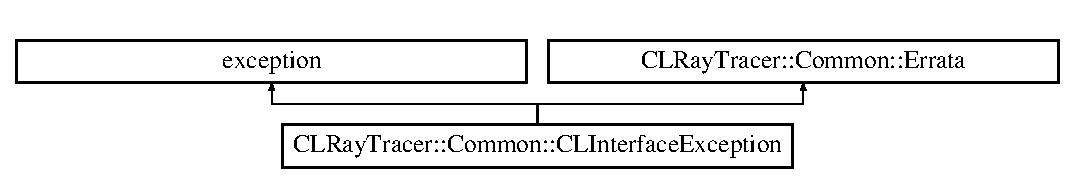
\includegraphics[height=2.000000cm]{class_c_l_ray_tracer_1_1_common_1_1_c_l_interface_exception}
\end{center}
\end{figure}
\subsection*{Public Member Functions}
\begin{DoxyCompactItemize}
\item 
\hyperlink{class_c_l_ray_tracer_1_1_common_1_1_c_l_interface_exception_a9d5f6bb82221341eb9ac7288d32af05b}{C\+L\+Interface\+Exception} (const std\+::string \&error\+Message, const std\+::string \&\hyperlink{class_c_l_ray_tracer_1_1_common_1_1_errata_ab02c644698211e5b40a9eb8504c4ebfa}{file}, const std\+::string \&\hyperlink{class_c_l_ray_tracer_1_1_common_1_1_errata_ac591fef29757e5309cefa5f96e2f647f}{function}, int \hyperlink{class_c_l_ray_tracer_1_1_common_1_1_errata_ae53b458949d7a8b1438f72086dee9d6d}{line}, std\+::exception $\ast$ex=N\+U\+LL)
\item 
\hyperlink{class_c_l_ray_tracer_1_1_common_1_1_c_l_interface_exception_a6cc2e89ab7ff12ace94e1ccc5678ca9d}{C\+L\+Interface\+Exception} (const \hyperlink{class_c_l_ray_tracer_1_1_common_1_1_errata}{Errata} \&err)
\end{DoxyCompactItemize}
\subsection*{Additional Inherited Members}


\subsection{Detailed Description}
class \hyperlink{class_c_l_ray_tracer_1_1_common_1_1_c_l_interface_exception}{C\+L\+Interface\+Exception} extends class \hyperlink{class_c_l_ray_tracer_1_1_common_1_1_errata}{Errata} to be throwable as exception 

\subsection{Constructor \& Destructor Documentation}
\index{C\+L\+Ray\+Tracer\+::\+Common\+::\+C\+L\+Interface\+Exception@{C\+L\+Ray\+Tracer\+::\+Common\+::\+C\+L\+Interface\+Exception}!C\+L\+Interface\+Exception@{C\+L\+Interface\+Exception}}
\index{C\+L\+Interface\+Exception@{C\+L\+Interface\+Exception}!C\+L\+Ray\+Tracer\+::\+Common\+::\+C\+L\+Interface\+Exception@{C\+L\+Ray\+Tracer\+::\+Common\+::\+C\+L\+Interface\+Exception}}
\subsubsection[{\texorpdfstring{C\+L\+Interface\+Exception(const std\+::string \&error\+Message, const std\+::string \&file, const std\+::string \&function, int line, std\+::exception $\ast$ex=\+N\+U\+L\+L)}{CLInterfaceException(const std::string &errorMessage, const std::string &file, const std::string &function, int line, std::exception *ex=NULL)}}]{\setlength{\rightskip}{0pt plus 5cm}C\+L\+Ray\+Tracer\+::\+Common\+::\+C\+L\+Interface\+Exception\+::\+C\+L\+Interface\+Exception (
\begin{DoxyParamCaption}
\item[{const std\+::string \&}]{error\+Message, }
\item[{const std\+::string \&}]{file, }
\item[{const std\+::string \&}]{function, }
\item[{int}]{line, }
\item[{std\+::exception $\ast$}]{ex = {\ttfamily NULL}}
\end{DoxyParamCaption}
)\hspace{0.3cm}{\ttfamily [inline]}}\hypertarget{class_c_l_ray_tracer_1_1_common_1_1_c_l_interface_exception_a9d5f6bb82221341eb9ac7288d32af05b}{}\label{class_c_l_ray_tracer_1_1_common_1_1_c_l_interface_exception_a9d5f6bb82221341eb9ac7288d32af05b}
Constructor 
\begin{DoxyParams}{Parameters}
{\em error\+Message} & The error message \\
\hline
{\em file} & Code file name, in which the error had occurred \\
\hline
{\em function} & Function in which the error occurred \\
\hline
{\em line} & Line in which the error had occurred \\
\hline
{\em \mbox{[}optional\mbox{]}exception} & Exception that caused the error \\
\hline
\end{DoxyParams}
\index{C\+L\+Ray\+Tracer\+::\+Common\+::\+C\+L\+Interface\+Exception@{C\+L\+Ray\+Tracer\+::\+Common\+::\+C\+L\+Interface\+Exception}!C\+L\+Interface\+Exception@{C\+L\+Interface\+Exception}}
\index{C\+L\+Interface\+Exception@{C\+L\+Interface\+Exception}!C\+L\+Ray\+Tracer\+::\+Common\+::\+C\+L\+Interface\+Exception@{C\+L\+Ray\+Tracer\+::\+Common\+::\+C\+L\+Interface\+Exception}}
\subsubsection[{\texorpdfstring{C\+L\+Interface\+Exception(const Errata \&err)}{CLInterfaceException(const Errata &err)}}]{\setlength{\rightskip}{0pt plus 5cm}C\+L\+Ray\+Tracer\+::\+Common\+::\+C\+L\+Interface\+Exception\+::\+C\+L\+Interface\+Exception (
\begin{DoxyParamCaption}
\item[{const {\bf Errata} \&}]{err}
\end{DoxyParamCaption}
)\hspace{0.3cm}{\ttfamily [inline]}}\hypertarget{class_c_l_ray_tracer_1_1_common_1_1_c_l_interface_exception_a6cc2e89ab7ff12ace94e1ccc5678ca9d}{}\label{class_c_l_ray_tracer_1_1_common_1_1_c_l_interface_exception_a6cc2e89ab7ff12ace94e1ccc5678ca9d}
Constructor that creates Exception from \hyperlink{class_c_l_ray_tracer_1_1_common_1_1_errata}{Errata} object 

The documentation for this class was generated from the following file\+:\begin{DoxyCompactItemize}
\item 
Include/\+Common/\hyperlink{_errata_8h}{Errata.\+h}\end{DoxyCompactItemize}

\hypertarget{class_c_l_ray_tracer_1_1_open_c_l_utils_1_1_c_l_kernel}{}\section{C\+L\+Ray\+Tracer\+:\+:Open\+C\+L\+Utils\+:\+:C\+L\+Kernel Class Reference}
\label{class_c_l_ray_tracer_1_1_open_c_l_utils_1_1_c_l_kernel}\index{C\+L\+Ray\+Tracer\+::\+Open\+C\+L\+Utils\+::\+C\+L\+Kernel@{C\+L\+Ray\+Tracer\+::\+Open\+C\+L\+Utils\+::\+C\+L\+Kernel}}


{\ttfamily \#include $<$C\+L\+Execution\+Context.\+h$>$}

\subsection*{Public Member Functions}
\begin{DoxyCompactItemize}
\item 
\hyperlink{class_c_l_ray_tracer_1_1_open_c_l_utils_1_1_c_l_kernel_a8c5fdaeb3a112507faf5c9a95b02ef8d}{C\+L\+Kernel} (cl\+\_\+kernel kernel)
\item 
\hyperlink{_errata_8h_a389396702f1aff6e71eb21328b0775c1}{Common\+::\+Result} \hyperlink{class_c_l_ray_tracer_1_1_open_c_l_utils_1_1_c_l_kernel_a126513da641d225be2ba05244305b74d}{set\+Kernel\+Argument} (const \hyperlink{class_c_l_ray_tracer_1_1_open_c_l_utils_1_1_c_l_kernel_argument}{C\+L\+Kernel\+Argument} \&arg\+Obj, cl\+\_\+uint index, \hyperlink{class_c_l_ray_tracer_1_1_common_1_1_errata}{Common\+::\+Errata} \&err)
\item 
virtual \hyperlink{class_c_l_ray_tracer_1_1_open_c_l_utils_1_1_c_l_kernel_ae21951d1144d8d39a88a1f1974c8b49d}{$\sim$\+C\+L\+Kernel} ()
\end{DoxyCompactItemize}
\subsection*{Protected Attributes}
\begin{DoxyCompactItemize}
\item 
cl\+\_\+kernel {\bfseries \+\_\+cl\+Kernel}\hypertarget{class_c_l_ray_tracer_1_1_open_c_l_utils_1_1_c_l_kernel_a7efb48091487bd104b949e18fa8785b1}{}\label{class_c_l_ray_tracer_1_1_open_c_l_utils_1_1_c_l_kernel_a7efb48091487bd104b949e18fa8785b1}

\end{DoxyCompactItemize}
\subsection*{Friends}
\begin{DoxyCompactItemize}
\item 
class {\bfseries C\+L\+Execution\+Context}\hypertarget{class_c_l_ray_tracer_1_1_open_c_l_utils_1_1_c_l_kernel_a778f7cdb701cc5559fd9c919558d70e7}{}\label{class_c_l_ray_tracer_1_1_open_c_l_utils_1_1_c_l_kernel_a778f7cdb701cc5559fd9c919558d70e7}

\end{DoxyCompactItemize}


\subsection{Detailed Description}
class \hyperlink{class_c_l_ray_tracer_1_1_open_c_l_utils_1_1_c_l_kernel}{C\+L\+Kernel} encapsulates the Open\+CL kernel 

\subsection{Constructor \& Destructor Documentation}
\index{C\+L\+Ray\+Tracer\+::\+Open\+C\+L\+Utils\+::\+C\+L\+Kernel@{C\+L\+Ray\+Tracer\+::\+Open\+C\+L\+Utils\+::\+C\+L\+Kernel}!C\+L\+Kernel@{C\+L\+Kernel}}
\index{C\+L\+Kernel@{C\+L\+Kernel}!C\+L\+Ray\+Tracer\+::\+Open\+C\+L\+Utils\+::\+C\+L\+Kernel@{C\+L\+Ray\+Tracer\+::\+Open\+C\+L\+Utils\+::\+C\+L\+Kernel}}
\subsubsection[{\texorpdfstring{C\+L\+Kernel(cl\+\_\+kernel kernel)}{CLKernel(cl_kernel kernel)}}]{\setlength{\rightskip}{0pt plus 5cm}C\+L\+Ray\+Tracer\+::\+Open\+C\+L\+Utils\+::\+C\+L\+Kernel\+::\+C\+L\+Kernel (
\begin{DoxyParamCaption}
\item[{cl\+\_\+kernel}]{kernel}
\end{DoxyParamCaption}
)}\hypertarget{class_c_l_ray_tracer_1_1_open_c_l_utils_1_1_c_l_kernel_a8c5fdaeb3a112507faf5c9a95b02ef8d}{}\label{class_c_l_ray_tracer_1_1_open_c_l_utils_1_1_c_l_kernel_a8c5fdaeb3a112507faf5c9a95b02ef8d}
Constructor 
\begin{DoxyParams}{Parameters}
{\em kernel} & The raw Open\+CL kernel object \\
\hline
\end{DoxyParams}
\index{C\+L\+Ray\+Tracer\+::\+Open\+C\+L\+Utils\+::\+C\+L\+Kernel@{C\+L\+Ray\+Tracer\+::\+Open\+C\+L\+Utils\+::\+C\+L\+Kernel}!````~C\+L\+Kernel@{$\sim$\+C\+L\+Kernel}}
\index{````~C\+L\+Kernel@{$\sim$\+C\+L\+Kernel}!C\+L\+Ray\+Tracer\+::\+Open\+C\+L\+Utils\+::\+C\+L\+Kernel@{C\+L\+Ray\+Tracer\+::\+Open\+C\+L\+Utils\+::\+C\+L\+Kernel}}
\subsubsection[{\texorpdfstring{$\sim$\+C\+L\+Kernel()}{~CLKernel()}}]{\setlength{\rightskip}{0pt plus 5cm}virtual C\+L\+Ray\+Tracer\+::\+Open\+C\+L\+Utils\+::\+C\+L\+Kernel\+::$\sim$\+C\+L\+Kernel (
\begin{DoxyParamCaption}
{}
\end{DoxyParamCaption}
)\hspace{0.3cm}{\ttfamily [virtual]}}\hypertarget{class_c_l_ray_tracer_1_1_open_c_l_utils_1_1_c_l_kernel_ae21951d1144d8d39a88a1f1974c8b49d}{}\label{class_c_l_ray_tracer_1_1_open_c_l_utils_1_1_c_l_kernel_ae21951d1144d8d39a88a1f1974c8b49d}
Destructor 

\subsection{Member Function Documentation}
\index{C\+L\+Ray\+Tracer\+::\+Open\+C\+L\+Utils\+::\+C\+L\+Kernel@{C\+L\+Ray\+Tracer\+::\+Open\+C\+L\+Utils\+::\+C\+L\+Kernel}!set\+Kernel\+Argument@{set\+Kernel\+Argument}}
\index{set\+Kernel\+Argument@{set\+Kernel\+Argument}!C\+L\+Ray\+Tracer\+::\+Open\+C\+L\+Utils\+::\+C\+L\+Kernel@{C\+L\+Ray\+Tracer\+::\+Open\+C\+L\+Utils\+::\+C\+L\+Kernel}}
\subsubsection[{\texorpdfstring{set\+Kernel\+Argument(const C\+L\+Kernel\+Argument \&arg\+Obj, cl\+\_\+uint index, Common\+::\+Errata \&err)}{setKernelArgument(const CLKernelArgument &argObj, cl_uint index, Common::Errata &err)}}]{\setlength{\rightskip}{0pt plus 5cm}{\bf Common\+::\+Result} C\+L\+Ray\+Tracer\+::\+Open\+C\+L\+Utils\+::\+C\+L\+Kernel\+::set\+Kernel\+Argument (
\begin{DoxyParamCaption}
\item[{const {\bf C\+L\+Kernel\+Argument} \&}]{arg\+Obj, }
\item[{cl\+\_\+uint}]{index, }
\item[{{\bf Common\+::\+Errata} \&}]{err}
\end{DoxyParamCaption}
)}\hypertarget{class_c_l_ray_tracer_1_1_open_c_l_utils_1_1_c_l_kernel_a126513da641d225be2ba05244305b74d}{}\label{class_c_l_ray_tracer_1_1_open_c_l_utils_1_1_c_l_kernel_a126513da641d225be2ba05244305b74d}
Sets argument value for this kernel 
\begin{DoxyParams}{Parameters}
{\em arg\+Obj} & Object that encapsulates the argument value \\
\hline
{\em Index} & at which the argument should be set \\
\hline
{\em err} & Error info \\
\hline
\end{DoxyParams}
\begin{DoxyReturn}{Returns}
Result of the operation\+: Success or failure 
\end{DoxyReturn}


The documentation for this class was generated from the following file\+:\begin{DoxyCompactItemize}
\item 
Include/\+Open\+C\+L\+Utils/\hyperlink{_c_l_execution_context_8h}{C\+L\+Execution\+Context.\+h}\end{DoxyCompactItemize}

\hypertarget{class_c_l_ray_tracer_1_1_open_c_l_utils_1_1_c_l_kernel_argument}{}\section{C\+L\+Ray\+Tracer\+:\+:Open\+C\+L\+Utils\+:\+:C\+L\+Kernel\+Argument Class Reference}
\label{class_c_l_ray_tracer_1_1_open_c_l_utils_1_1_c_l_kernel_argument}\index{C\+L\+Ray\+Tracer\+::\+Open\+C\+L\+Utils\+::\+C\+L\+Kernel\+Argument@{C\+L\+Ray\+Tracer\+::\+Open\+C\+L\+Utils\+::\+C\+L\+Kernel\+Argument}}


{\ttfamily \#include $<$C\+L\+Execution\+Context.\+h$>$}

\subsection*{Public Member Functions}
\begin{DoxyCompactItemize}
\item 
{\footnotesize template$<$class T $>$ }\\\hyperlink{class_c_l_ray_tracer_1_1_open_c_l_utils_1_1_c_l_kernel_argument_ad4a2f6eeb0021cc7af9bffed5ffad0f0}{C\+L\+Kernel\+Argument} (const T \&data)
\item 
\hyperlink{class_c_l_ray_tracer_1_1_open_c_l_utils_1_1_c_l_kernel_argument_a8c1b6453792f8623bb9e03f112ce48ae}{C\+L\+Kernel\+Argument} (cl\+\_\+uint local\+Mem\+Size)
\item 
void $\ast$ \hyperlink{class_c_l_ray_tracer_1_1_open_c_l_utils_1_1_c_l_kernel_argument_a9a9131d7c5dbdfcae7187e559ef18bd8}{get\+Void\+Ptr} () const 
\item 
size\+\_\+t \hyperlink{class_c_l_ray_tracer_1_1_open_c_l_utils_1_1_c_l_kernel_argument_ac563b112959bf8b66e875e017b60f196}{get\+Data\+Size} () const 
\item 
bool \hyperlink{class_c_l_ray_tracer_1_1_open_c_l_utils_1_1_c_l_kernel_argument_aa32628bdad331d091ca2b31b053dabff}{is\+Dummy} () const 
\end{DoxyCompactItemize}
\subsection*{Static Public Attributes}
\begin{DoxyCompactItemize}
\item 
static const char $\ast$ \hyperlink{class_c_l_ray_tracer_1_1_open_c_l_utils_1_1_c_l_kernel_argument_a08d988445003da2332783b18eef8f23f}{Dummy\+Arg}
\end{DoxyCompactItemize}


\subsection{Detailed Description}
class \hyperlink{class_c_l_ray_tracer_1_1_open_c_l_utils_1_1_c_l_kernel_argument}{C\+L\+Kernel\+Argument} encapsulates an argument to Open\+CL kernel 

\subsection{Constructor \& Destructor Documentation}
\index{C\+L\+Ray\+Tracer\+::\+Open\+C\+L\+Utils\+::\+C\+L\+Kernel\+Argument@{C\+L\+Ray\+Tracer\+::\+Open\+C\+L\+Utils\+::\+C\+L\+Kernel\+Argument}!C\+L\+Kernel\+Argument@{C\+L\+Kernel\+Argument}}
\index{C\+L\+Kernel\+Argument@{C\+L\+Kernel\+Argument}!C\+L\+Ray\+Tracer\+::\+Open\+C\+L\+Utils\+::\+C\+L\+Kernel\+Argument@{C\+L\+Ray\+Tracer\+::\+Open\+C\+L\+Utils\+::\+C\+L\+Kernel\+Argument}}
\subsubsection[{\texorpdfstring{C\+L\+Kernel\+Argument(const T \&data)}{CLKernelArgument(const T &data)}}]{\setlength{\rightskip}{0pt plus 5cm}template$<$class T $>$ C\+L\+Ray\+Tracer\+::\+Open\+C\+L\+Utils\+::\+C\+L\+Kernel\+Argument\+::\+C\+L\+Kernel\+Argument (
\begin{DoxyParamCaption}
\item[{const T \&}]{data}
\end{DoxyParamCaption}
)\hspace{0.3cm}{\ttfamily [inline]}}\hypertarget{class_c_l_ray_tracer_1_1_open_c_l_utils_1_1_c_l_kernel_argument_ad4a2f6eeb0021cc7af9bffed5ffad0f0}{}\label{class_c_l_ray_tracer_1_1_open_c_l_utils_1_1_c_l_kernel_argument_ad4a2f6eeb0021cc7af9bffed5ffad0f0}
Constructor -\/ Allows implicit initialization with any type \index{C\+L\+Ray\+Tracer\+::\+Open\+C\+L\+Utils\+::\+C\+L\+Kernel\+Argument@{C\+L\+Ray\+Tracer\+::\+Open\+C\+L\+Utils\+::\+C\+L\+Kernel\+Argument}!C\+L\+Kernel\+Argument@{C\+L\+Kernel\+Argument}}
\index{C\+L\+Kernel\+Argument@{C\+L\+Kernel\+Argument}!C\+L\+Ray\+Tracer\+::\+Open\+C\+L\+Utils\+::\+C\+L\+Kernel\+Argument@{C\+L\+Ray\+Tracer\+::\+Open\+C\+L\+Utils\+::\+C\+L\+Kernel\+Argument}}
\subsubsection[{\texorpdfstring{C\+L\+Kernel\+Argument(cl\+\_\+uint local\+Mem\+Size)}{CLKernelArgument(cl_uint localMemSize)}}]{\setlength{\rightskip}{0pt plus 5cm}C\+L\+Ray\+Tracer\+::\+Open\+C\+L\+Utils\+::\+C\+L\+Kernel\+Argument\+::\+C\+L\+Kernel\+Argument (
\begin{DoxyParamCaption}
\item[{cl\+\_\+uint}]{local\+Mem\+Size}
\end{DoxyParamCaption}
)\hspace{0.3cm}{\ttfamily [inline]}, {\ttfamily [explicit]}}\hypertarget{class_c_l_ray_tracer_1_1_open_c_l_utils_1_1_c_l_kernel_argument_a8c1b6453792f8623bb9e03f112ce48ae}{}\label{class_c_l_ray_tracer_1_1_open_c_l_utils_1_1_c_l_kernel_argument_a8c1b6453792f8623bb9e03f112ce48ae}
Constructor for local memory allocation 

\subsection{Member Function Documentation}
\index{C\+L\+Ray\+Tracer\+::\+Open\+C\+L\+Utils\+::\+C\+L\+Kernel\+Argument@{C\+L\+Ray\+Tracer\+::\+Open\+C\+L\+Utils\+::\+C\+L\+Kernel\+Argument}!get\+Data\+Size@{get\+Data\+Size}}
\index{get\+Data\+Size@{get\+Data\+Size}!C\+L\+Ray\+Tracer\+::\+Open\+C\+L\+Utils\+::\+C\+L\+Kernel\+Argument@{C\+L\+Ray\+Tracer\+::\+Open\+C\+L\+Utils\+::\+C\+L\+Kernel\+Argument}}
\subsubsection[{\texorpdfstring{get\+Data\+Size() const }{getDataSize() const }}]{\setlength{\rightskip}{0pt plus 5cm}size\+\_\+t C\+L\+Ray\+Tracer\+::\+Open\+C\+L\+Utils\+::\+C\+L\+Kernel\+Argument\+::get\+Data\+Size (
\begin{DoxyParamCaption}
{}
\end{DoxyParamCaption}
) const\hspace{0.3cm}{\ttfamily [inline]}}\hypertarget{class_c_l_ray_tracer_1_1_open_c_l_utils_1_1_c_l_kernel_argument_ac563b112959bf8b66e875e017b60f196}{}\label{class_c_l_ray_tracer_1_1_open_c_l_utils_1_1_c_l_kernel_argument_ac563b112959bf8b66e875e017b60f196}
Returns argument data size in bytes \begin{DoxyReturn}{Returns}
Argument data size in bytes 
\end{DoxyReturn}
\index{C\+L\+Ray\+Tracer\+::\+Open\+C\+L\+Utils\+::\+C\+L\+Kernel\+Argument@{C\+L\+Ray\+Tracer\+::\+Open\+C\+L\+Utils\+::\+C\+L\+Kernel\+Argument}!get\+Void\+Ptr@{get\+Void\+Ptr}}
\index{get\+Void\+Ptr@{get\+Void\+Ptr}!C\+L\+Ray\+Tracer\+::\+Open\+C\+L\+Utils\+::\+C\+L\+Kernel\+Argument@{C\+L\+Ray\+Tracer\+::\+Open\+C\+L\+Utils\+::\+C\+L\+Kernel\+Argument}}
\subsubsection[{\texorpdfstring{get\+Void\+Ptr() const }{getVoidPtr() const }}]{\setlength{\rightskip}{0pt plus 5cm}void$\ast$ C\+L\+Ray\+Tracer\+::\+Open\+C\+L\+Utils\+::\+C\+L\+Kernel\+Argument\+::get\+Void\+Ptr (
\begin{DoxyParamCaption}
{}
\end{DoxyParamCaption}
) const\hspace{0.3cm}{\ttfamily [inline]}}\hypertarget{class_c_l_ray_tracer_1_1_open_c_l_utils_1_1_c_l_kernel_argument_a9a9131d7c5dbdfcae7187e559ef18bd8}{}\label{class_c_l_ray_tracer_1_1_open_c_l_utils_1_1_c_l_kernel_argument_a9a9131d7c5dbdfcae7187e559ef18bd8}
Returns pointer to data encapsulated in the kernel argument wrapper \begin{DoxyReturn}{Returns}
Pointer to data encapsulated in the kernel argument wrapper 
\end{DoxyReturn}
\index{C\+L\+Ray\+Tracer\+::\+Open\+C\+L\+Utils\+::\+C\+L\+Kernel\+Argument@{C\+L\+Ray\+Tracer\+::\+Open\+C\+L\+Utils\+::\+C\+L\+Kernel\+Argument}!is\+Dummy@{is\+Dummy}}
\index{is\+Dummy@{is\+Dummy}!C\+L\+Ray\+Tracer\+::\+Open\+C\+L\+Utils\+::\+C\+L\+Kernel\+Argument@{C\+L\+Ray\+Tracer\+::\+Open\+C\+L\+Utils\+::\+C\+L\+Kernel\+Argument}}
\subsubsection[{\texorpdfstring{is\+Dummy() const }{isDummy() const }}]{\setlength{\rightskip}{0pt plus 5cm}bool C\+L\+Ray\+Tracer\+::\+Open\+C\+L\+Utils\+::\+C\+L\+Kernel\+Argument\+::is\+Dummy (
\begin{DoxyParamCaption}
{}
\end{DoxyParamCaption}
) const\hspace{0.3cm}{\ttfamily [inline]}}\hypertarget{class_c_l_ray_tracer_1_1_open_c_l_utils_1_1_c_l_kernel_argument_aa32628bdad331d091ca2b31b053dabff}{}\label{class_c_l_ray_tracer_1_1_open_c_l_utils_1_1_c_l_kernel_argument_aa32628bdad331d091ca2b31b053dabff}
Indicates whether this argument is a dummy argument \begin{DoxyReturn}{Returns}
True if the argument is a Dummy argument 
\end{DoxyReturn}


\subsection{Member Data Documentation}
\index{C\+L\+Ray\+Tracer\+::\+Open\+C\+L\+Utils\+::\+C\+L\+Kernel\+Argument@{C\+L\+Ray\+Tracer\+::\+Open\+C\+L\+Utils\+::\+C\+L\+Kernel\+Argument}!Dummy\+Arg@{Dummy\+Arg}}
\index{Dummy\+Arg@{Dummy\+Arg}!C\+L\+Ray\+Tracer\+::\+Open\+C\+L\+Utils\+::\+C\+L\+Kernel\+Argument@{C\+L\+Ray\+Tracer\+::\+Open\+C\+L\+Utils\+::\+C\+L\+Kernel\+Argument}}
\subsubsection[{\texorpdfstring{Dummy\+Arg}{DummyArg}}]{\setlength{\rightskip}{0pt plus 5cm}const char$\ast$ C\+L\+Ray\+Tracer\+::\+Open\+C\+L\+Utils\+::\+C\+L\+Kernel\+Argument\+::\+Dummy\+Arg\hspace{0.3cm}{\ttfamily [static]}}\hypertarget{class_c_l_ray_tracer_1_1_open_c_l_utils_1_1_c_l_kernel_argument_a08d988445003da2332783b18eef8f23f}{}\label{class_c_l_ray_tracer_1_1_open_c_l_utils_1_1_c_l_kernel_argument_a08d988445003da2332783b18eef8f23f}
Dummy argument 

The documentation for this class was generated from the following file\+:\begin{DoxyCompactItemize}
\item 
Include/\+Open\+C\+L\+Utils/\hyperlink{_c_l_execution_context_8h}{C\+L\+Execution\+Context.\+h}\end{DoxyCompactItemize}

\hypertarget{class_c_l_ray_tracer_1_1_open_c_l_utils_1_1_c_l_kernel_execute_params}{}\section{C\+L\+Ray\+Tracer\+:\+:Open\+C\+L\+Utils\+:\+:C\+L\+Kernel\+Execute\+Params Class Reference}
\label{class_c_l_ray_tracer_1_1_open_c_l_utils_1_1_c_l_kernel_execute_params}\index{C\+L\+Ray\+Tracer\+::\+Open\+C\+L\+Utils\+::\+C\+L\+Kernel\+Execute\+Params@{C\+L\+Ray\+Tracer\+::\+Open\+C\+L\+Utils\+::\+C\+L\+Kernel\+Execute\+Params}}


{\ttfamily \#include $<$C\+L\+Execution\+Context.\+h$>$}

\subsection*{Public Member Functions}
\begin{DoxyCompactItemize}
\item 
\hyperlink{class_c_l_ray_tracer_1_1_open_c_l_utils_1_1_c_l_kernel_execute_params_a3b459bbfe18d2659f172c451a30107a5}{C\+L\+Kernel\+Execute\+Params} (\hyperlink{class_c_l_ray_tracer_1_1_open_c_l_utils_1_1_c_l_kernel_work_dimension}{C\+L\+Kernel\+Work\+Dimension} $\ast$global\+WD, \hyperlink{class_c_l_ray_tracer_1_1_open_c_l_utils_1_1_c_l_kernel_work_dimension}{C\+L\+Kernel\+Work\+Dimension} $\ast$local\+WD, \hyperlink{class_c_l_ray_tracer_1_1_open_c_l_utils_1_1_c_l_event}{C\+L\+Event} $\ast$evt=N\+U\+LL)
\item 
void \hyperlink{class_c_l_ray_tracer_1_1_open_c_l_utils_1_1_c_l_kernel_execute_params_a862d87802bc433ac8acf1cd3eeed71d4}{add\+Event\+To\+Wait\+List} (\hyperlink{class_c_l_ray_tracer_1_1_open_c_l_utils_1_1_c_l_event}{C\+L\+Event} evt)
\end{DoxyCompactItemize}
\subsection*{Public Attributes}
\begin{DoxyCompactItemize}
\item 
\hyperlink{class_c_l_ray_tracer_1_1_open_c_l_utils_1_1_c_l_event}{C\+L\+Event} $\ast$ \hyperlink{class_c_l_ray_tracer_1_1_open_c_l_utils_1_1_c_l_kernel_execute_params_a8debf260792693a64c01904ed43004c3}{event}
\item 
\hyperlink{class_c_l_ray_tracer_1_1_open_c_l_utils_1_1_c_l_kernel_work_dimension}{C\+L\+Kernel\+Work\+Dimension} $\ast$ \hyperlink{class_c_l_ray_tracer_1_1_open_c_l_utils_1_1_c_l_kernel_execute_params_ae0daedd4a1726c9ffa43b38f8e6c9920}{local\+Work\+Dimension}
\item 
\hyperlink{class_c_l_ray_tracer_1_1_open_c_l_utils_1_1_c_l_kernel_work_dimension}{C\+L\+Kernel\+Work\+Dimension} $\ast$ \hyperlink{class_c_l_ray_tracer_1_1_open_c_l_utils_1_1_c_l_kernel_execute_params_af62889e5fd651360d69ee92e23977bda}{global\+Work\+Dimension}
\item 
\hyperlink{class_c_l_ray_tracer_1_1_open_c_l_utils_1_1_c_l_kernel_work_dimension}{C\+L\+Kernel\+Work\+Dimension} $\ast$ \hyperlink{class_c_l_ray_tracer_1_1_open_c_l_utils_1_1_c_l_kernel_execute_params_aeaddbee87bcc68e36a78b517c8cddbd8}{global\+Work\+Offset}
\item 
std\+::vector$<$ cl\+\_\+event $>$ \hyperlink{class_c_l_ray_tracer_1_1_open_c_l_utils_1_1_c_l_kernel_execute_params_a2319b0deec1732ec481a75d4b188f789}{event\+Wait\+List}
\end{DoxyCompactItemize}


\subsection{Detailed Description}
class C\+L\+Kernel\+Execution\+Params encapsulates the work dimensions for kernel execution 

\subsection{Constructor \& Destructor Documentation}
\index{C\+L\+Ray\+Tracer\+::\+Open\+C\+L\+Utils\+::\+C\+L\+Kernel\+Execute\+Params@{C\+L\+Ray\+Tracer\+::\+Open\+C\+L\+Utils\+::\+C\+L\+Kernel\+Execute\+Params}!C\+L\+Kernel\+Execute\+Params@{C\+L\+Kernel\+Execute\+Params}}
\index{C\+L\+Kernel\+Execute\+Params@{C\+L\+Kernel\+Execute\+Params}!C\+L\+Ray\+Tracer\+::\+Open\+C\+L\+Utils\+::\+C\+L\+Kernel\+Execute\+Params@{C\+L\+Ray\+Tracer\+::\+Open\+C\+L\+Utils\+::\+C\+L\+Kernel\+Execute\+Params}}
\subsubsection[{\texorpdfstring{C\+L\+Kernel\+Execute\+Params(\+C\+L\+Kernel\+Work\+Dimension $\ast$global\+W\+D, C\+L\+Kernel\+Work\+Dimension $\ast$local\+W\+D, C\+L\+Event $\ast$evt=\+N\+U\+L\+L)}{CLKernelExecuteParams(CLKernelWorkDimension *globalWD, CLKernelWorkDimension *localWD, CLEvent *evt=NULL)}}]{\setlength{\rightskip}{0pt plus 5cm}C\+L\+Ray\+Tracer\+::\+Open\+C\+L\+Utils\+::\+C\+L\+Kernel\+Execute\+Params\+::\+C\+L\+Kernel\+Execute\+Params (
\begin{DoxyParamCaption}
\item[{{\bf C\+L\+Kernel\+Work\+Dimension} $\ast$}]{global\+WD, }
\item[{{\bf C\+L\+Kernel\+Work\+Dimension} $\ast$}]{local\+WD, }
\item[{{\bf C\+L\+Event} $\ast$}]{evt = {\ttfamily NULL}}
\end{DoxyParamCaption}
)\hspace{0.3cm}{\ttfamily [inline]}}\hypertarget{class_c_l_ray_tracer_1_1_open_c_l_utils_1_1_c_l_kernel_execute_params_a3b459bbfe18d2659f172c451a30107a5}{}\label{class_c_l_ray_tracer_1_1_open_c_l_utils_1_1_c_l_kernel_execute_params_a3b459bbfe18d2659f172c451a30107a5}
Constructor 
\begin{DoxyParams}{Parameters}
{\em global\+WD} & Global work dimension \\
\hline
{\em local\+WD} & Local work dimension \\
\hline
{\em \mbox{[}optional\mbox{]}evt} & Synchronization event associated with kernel execution \\
\hline
\end{DoxyParams}


\subsection{Member Function Documentation}
\index{C\+L\+Ray\+Tracer\+::\+Open\+C\+L\+Utils\+::\+C\+L\+Kernel\+Execute\+Params@{C\+L\+Ray\+Tracer\+::\+Open\+C\+L\+Utils\+::\+C\+L\+Kernel\+Execute\+Params}!add\+Event\+To\+Wait\+List@{add\+Event\+To\+Wait\+List}}
\index{add\+Event\+To\+Wait\+List@{add\+Event\+To\+Wait\+List}!C\+L\+Ray\+Tracer\+::\+Open\+C\+L\+Utils\+::\+C\+L\+Kernel\+Execute\+Params@{C\+L\+Ray\+Tracer\+::\+Open\+C\+L\+Utils\+::\+C\+L\+Kernel\+Execute\+Params}}
\subsubsection[{\texorpdfstring{add\+Event\+To\+Wait\+List(\+C\+L\+Event evt)}{addEventToWaitList(CLEvent evt)}}]{\setlength{\rightskip}{0pt plus 5cm}void C\+L\+Ray\+Tracer\+::\+Open\+C\+L\+Utils\+::\+C\+L\+Kernel\+Execute\+Params\+::add\+Event\+To\+Wait\+List (
\begin{DoxyParamCaption}
\item[{{\bf C\+L\+Event}}]{evt}
\end{DoxyParamCaption}
)\hspace{0.3cm}{\ttfamily [inline]}}\hypertarget{class_c_l_ray_tracer_1_1_open_c_l_utils_1_1_c_l_kernel_execute_params_a862d87802bc433ac8acf1cd3eeed71d4}{}\label{class_c_l_ray_tracer_1_1_open_c_l_utils_1_1_c_l_kernel_execute_params_a862d87802bc433ac8acf1cd3eeed71d4}
Adds the input event to event wait list for kernel execution 
\begin{DoxyParams}{Parameters}
{\em evt} & Event to add \\
\hline
\end{DoxyParams}
\begin{DoxyReturn}{Returns}

\end{DoxyReturn}


\subsection{Member Data Documentation}
\index{C\+L\+Ray\+Tracer\+::\+Open\+C\+L\+Utils\+::\+C\+L\+Kernel\+Execute\+Params@{C\+L\+Ray\+Tracer\+::\+Open\+C\+L\+Utils\+::\+C\+L\+Kernel\+Execute\+Params}!event@{event}}
\index{event@{event}!C\+L\+Ray\+Tracer\+::\+Open\+C\+L\+Utils\+::\+C\+L\+Kernel\+Execute\+Params@{C\+L\+Ray\+Tracer\+::\+Open\+C\+L\+Utils\+::\+C\+L\+Kernel\+Execute\+Params}}
\subsubsection[{\texorpdfstring{event}{event}}]{\setlength{\rightskip}{0pt plus 5cm}{\bf C\+L\+Event}$\ast$ C\+L\+Ray\+Tracer\+::\+Open\+C\+L\+Utils\+::\+C\+L\+Kernel\+Execute\+Params\+::event}\hypertarget{class_c_l_ray_tracer_1_1_open_c_l_utils_1_1_c_l_kernel_execute_params_a8debf260792693a64c01904ed43004c3}{}\label{class_c_l_ray_tracer_1_1_open_c_l_utils_1_1_c_l_kernel_execute_params_a8debf260792693a64c01904ed43004c3}
Event object (This class doesn\textquotesingle{}t have ownership on the object) \index{C\+L\+Ray\+Tracer\+::\+Open\+C\+L\+Utils\+::\+C\+L\+Kernel\+Execute\+Params@{C\+L\+Ray\+Tracer\+::\+Open\+C\+L\+Utils\+::\+C\+L\+Kernel\+Execute\+Params}!event\+Wait\+List@{event\+Wait\+List}}
\index{event\+Wait\+List@{event\+Wait\+List}!C\+L\+Ray\+Tracer\+::\+Open\+C\+L\+Utils\+::\+C\+L\+Kernel\+Execute\+Params@{C\+L\+Ray\+Tracer\+::\+Open\+C\+L\+Utils\+::\+C\+L\+Kernel\+Execute\+Params}}
\subsubsection[{\texorpdfstring{event\+Wait\+List}{eventWaitList}}]{\setlength{\rightskip}{0pt plus 5cm}std\+::vector$<$cl\+\_\+event$>$ C\+L\+Ray\+Tracer\+::\+Open\+C\+L\+Utils\+::\+C\+L\+Kernel\+Execute\+Params\+::event\+Wait\+List}\hypertarget{class_c_l_ray_tracer_1_1_open_c_l_utils_1_1_c_l_kernel_execute_params_a2319b0deec1732ec481a75d4b188f789}{}\label{class_c_l_ray_tracer_1_1_open_c_l_utils_1_1_c_l_kernel_execute_params_a2319b0deec1732ec481a75d4b188f789}
Event wait list for kernel execution \index{C\+L\+Ray\+Tracer\+::\+Open\+C\+L\+Utils\+::\+C\+L\+Kernel\+Execute\+Params@{C\+L\+Ray\+Tracer\+::\+Open\+C\+L\+Utils\+::\+C\+L\+Kernel\+Execute\+Params}!global\+Work\+Dimension@{global\+Work\+Dimension}}
\index{global\+Work\+Dimension@{global\+Work\+Dimension}!C\+L\+Ray\+Tracer\+::\+Open\+C\+L\+Utils\+::\+C\+L\+Kernel\+Execute\+Params@{C\+L\+Ray\+Tracer\+::\+Open\+C\+L\+Utils\+::\+C\+L\+Kernel\+Execute\+Params}}
\subsubsection[{\texorpdfstring{global\+Work\+Dimension}{globalWorkDimension}}]{\setlength{\rightskip}{0pt plus 5cm}{\bf C\+L\+Kernel\+Work\+Dimension}$\ast$ C\+L\+Ray\+Tracer\+::\+Open\+C\+L\+Utils\+::\+C\+L\+Kernel\+Execute\+Params\+::global\+Work\+Dimension}\hypertarget{class_c_l_ray_tracer_1_1_open_c_l_utils_1_1_c_l_kernel_execute_params_af62889e5fd651360d69ee92e23977bda}{}\label{class_c_l_ray_tracer_1_1_open_c_l_utils_1_1_c_l_kernel_execute_params_af62889e5fd651360d69ee92e23977bda}
Global work dimension (This class doesn\textquotesingle{}t have ownership on the object) \index{C\+L\+Ray\+Tracer\+::\+Open\+C\+L\+Utils\+::\+C\+L\+Kernel\+Execute\+Params@{C\+L\+Ray\+Tracer\+::\+Open\+C\+L\+Utils\+::\+C\+L\+Kernel\+Execute\+Params}!global\+Work\+Offset@{global\+Work\+Offset}}
\index{global\+Work\+Offset@{global\+Work\+Offset}!C\+L\+Ray\+Tracer\+::\+Open\+C\+L\+Utils\+::\+C\+L\+Kernel\+Execute\+Params@{C\+L\+Ray\+Tracer\+::\+Open\+C\+L\+Utils\+::\+C\+L\+Kernel\+Execute\+Params}}
\subsubsection[{\texorpdfstring{global\+Work\+Offset}{globalWorkOffset}}]{\setlength{\rightskip}{0pt plus 5cm}{\bf C\+L\+Kernel\+Work\+Dimension}$\ast$ C\+L\+Ray\+Tracer\+::\+Open\+C\+L\+Utils\+::\+C\+L\+Kernel\+Execute\+Params\+::global\+Work\+Offset}\hypertarget{class_c_l_ray_tracer_1_1_open_c_l_utils_1_1_c_l_kernel_execute_params_aeaddbee87bcc68e36a78b517c8cddbd8}{}\label{class_c_l_ray_tracer_1_1_open_c_l_utils_1_1_c_l_kernel_execute_params_aeaddbee87bcc68e36a78b517c8cddbd8}
Global work offset (This class doesn\textquotesingle{}t have ownership on the object) \index{C\+L\+Ray\+Tracer\+::\+Open\+C\+L\+Utils\+::\+C\+L\+Kernel\+Execute\+Params@{C\+L\+Ray\+Tracer\+::\+Open\+C\+L\+Utils\+::\+C\+L\+Kernel\+Execute\+Params}!local\+Work\+Dimension@{local\+Work\+Dimension}}
\index{local\+Work\+Dimension@{local\+Work\+Dimension}!C\+L\+Ray\+Tracer\+::\+Open\+C\+L\+Utils\+::\+C\+L\+Kernel\+Execute\+Params@{C\+L\+Ray\+Tracer\+::\+Open\+C\+L\+Utils\+::\+C\+L\+Kernel\+Execute\+Params}}
\subsubsection[{\texorpdfstring{local\+Work\+Dimension}{localWorkDimension}}]{\setlength{\rightskip}{0pt plus 5cm}{\bf C\+L\+Kernel\+Work\+Dimension}$\ast$ C\+L\+Ray\+Tracer\+::\+Open\+C\+L\+Utils\+::\+C\+L\+Kernel\+Execute\+Params\+::local\+Work\+Dimension}\hypertarget{class_c_l_ray_tracer_1_1_open_c_l_utils_1_1_c_l_kernel_execute_params_ae0daedd4a1726c9ffa43b38f8e6c9920}{}\label{class_c_l_ray_tracer_1_1_open_c_l_utils_1_1_c_l_kernel_execute_params_ae0daedd4a1726c9ffa43b38f8e6c9920}
Local work dimension (This class doesn\textquotesingle{}t have ownership on the object) 

The documentation for this class was generated from the following file\+:\begin{DoxyCompactItemize}
\item 
Include/\+Open\+C\+L\+Utils/\hyperlink{_c_l_execution_context_8h}{C\+L\+Execution\+Context.\+h}\end{DoxyCompactItemize}

\hypertarget{class_c_l_ray_tracer_1_1_open_c_l_utils_1_1_c_l_kernel_work_dimension}{}\section{C\+L\+Ray\+Tracer\+:\+:Open\+C\+L\+Utils\+:\+:C\+L\+Kernel\+Work\+Dimension Class Reference}
\label{class_c_l_ray_tracer_1_1_open_c_l_utils_1_1_c_l_kernel_work_dimension}\index{C\+L\+Ray\+Tracer\+::\+Open\+C\+L\+Utils\+::\+C\+L\+Kernel\+Work\+Dimension@{C\+L\+Ray\+Tracer\+::\+Open\+C\+L\+Utils\+::\+C\+L\+Kernel\+Work\+Dimension}}


{\ttfamily \#include $<$C\+L\+Execution\+Context.\+h$>$}

\subsection*{Public Member Functions}
\begin{DoxyCompactItemize}
\item 
\hyperlink{class_c_l_ray_tracer_1_1_open_c_l_utils_1_1_c_l_kernel_work_dimension_a16bab2ce5ac4dcc1f62072222af09a21}{C\+L\+Kernel\+Work\+Dimension} (cl\+\_\+uint work\+Dim,...)
\item 
unsigned int \hyperlink{class_c_l_ray_tracer_1_1_open_c_l_utils_1_1_c_l_kernel_work_dimension_a855d1646e6140f8a832b3bcffbcf0fb4}{total\+Items} () const 
\end{DoxyCompactItemize}
\subsection*{Public Attributes}
\begin{DoxyCompactItemize}
\item 
const cl\+\_\+uint \hyperlink{class_c_l_ray_tracer_1_1_open_c_l_utils_1_1_c_l_kernel_work_dimension_affd23924899b196276bedd7010af3e30}{work\+Dimensions}
\item 
const boost\+::shared\+\_\+array$<$ size\+\_\+t $>$ \hyperlink{class_c_l_ray_tracer_1_1_open_c_l_utils_1_1_c_l_kernel_work_dimension_aabe343f3cd0fb5a0320c73bb50a77ff0}{dimension\+Values}
\end{DoxyCompactItemize}


\subsection{Detailed Description}
class \hyperlink{class_c_l_ray_tracer_1_1_open_c_l_utils_1_1_c_l_kernel_work_dimension}{C\+L\+Kernel\+Work\+Dimension} encapsulates the work dimensions for Open\+CL kernel execution 

\subsection{Constructor \& Destructor Documentation}
\index{C\+L\+Ray\+Tracer\+::\+Open\+C\+L\+Utils\+::\+C\+L\+Kernel\+Work\+Dimension@{C\+L\+Ray\+Tracer\+::\+Open\+C\+L\+Utils\+::\+C\+L\+Kernel\+Work\+Dimension}!C\+L\+Kernel\+Work\+Dimension@{C\+L\+Kernel\+Work\+Dimension}}
\index{C\+L\+Kernel\+Work\+Dimension@{C\+L\+Kernel\+Work\+Dimension}!C\+L\+Ray\+Tracer\+::\+Open\+C\+L\+Utils\+::\+C\+L\+Kernel\+Work\+Dimension@{C\+L\+Ray\+Tracer\+::\+Open\+C\+L\+Utils\+::\+C\+L\+Kernel\+Work\+Dimension}}
\subsubsection[{\texorpdfstring{C\+L\+Kernel\+Work\+Dimension(cl\+\_\+uint work\+Dim,...)}{CLKernelWorkDimension(cl_uint workDim,...)}}]{\setlength{\rightskip}{0pt plus 5cm}C\+L\+Ray\+Tracer\+::\+Open\+C\+L\+Utils\+::\+C\+L\+Kernel\+Work\+Dimension\+::\+C\+L\+Kernel\+Work\+Dimension (
\begin{DoxyParamCaption}
\item[{cl\+\_\+uint}]{work\+Dim, }
\item[{}]{...}
\end{DoxyParamCaption}
)\hspace{0.3cm}{\ttfamily [inline]}}\hypertarget{class_c_l_ray_tracer_1_1_open_c_l_utils_1_1_c_l_kernel_work_dimension_a16bab2ce5ac4dcc1f62072222af09a21}{}\label{class_c_l_ray_tracer_1_1_open_c_l_utils_1_1_c_l_kernel_work_dimension_a16bab2ce5ac4dcc1f62072222af09a21}
Constructor 
\begin{DoxyParams}{Parameters}
{\em work\+Dim} & Number of work dimensions \\
\hline
{\em va\+\_\+arg} & Size of the work group along corresponding dimension \\
\hline
\end{DoxyParams}


\subsection{Member Function Documentation}
\index{C\+L\+Ray\+Tracer\+::\+Open\+C\+L\+Utils\+::\+C\+L\+Kernel\+Work\+Dimension@{C\+L\+Ray\+Tracer\+::\+Open\+C\+L\+Utils\+::\+C\+L\+Kernel\+Work\+Dimension}!total\+Items@{total\+Items}}
\index{total\+Items@{total\+Items}!C\+L\+Ray\+Tracer\+::\+Open\+C\+L\+Utils\+::\+C\+L\+Kernel\+Work\+Dimension@{C\+L\+Ray\+Tracer\+::\+Open\+C\+L\+Utils\+::\+C\+L\+Kernel\+Work\+Dimension}}
\subsubsection[{\texorpdfstring{total\+Items() const }{totalItems() const }}]{\setlength{\rightskip}{0pt plus 5cm}unsigned int C\+L\+Ray\+Tracer\+::\+Open\+C\+L\+Utils\+::\+C\+L\+Kernel\+Work\+Dimension\+::total\+Items (
\begin{DoxyParamCaption}
{}
\end{DoxyParamCaption}
) const\hspace{0.3cm}{\ttfamily [inline]}}\hypertarget{class_c_l_ray_tracer_1_1_open_c_l_utils_1_1_c_l_kernel_work_dimension_a855d1646e6140f8a832b3bcffbcf0fb4}{}\label{class_c_l_ray_tracer_1_1_open_c_l_utils_1_1_c_l_kernel_work_dimension_a855d1646e6140f8a832b3bcffbcf0fb4}
Counts total work items for Dimension object \begin{DoxyReturn}{Returns}
Sum of all items in all dimensions 
\end{DoxyReturn}


\subsection{Member Data Documentation}
\index{C\+L\+Ray\+Tracer\+::\+Open\+C\+L\+Utils\+::\+C\+L\+Kernel\+Work\+Dimension@{C\+L\+Ray\+Tracer\+::\+Open\+C\+L\+Utils\+::\+C\+L\+Kernel\+Work\+Dimension}!dimension\+Values@{dimension\+Values}}
\index{dimension\+Values@{dimension\+Values}!C\+L\+Ray\+Tracer\+::\+Open\+C\+L\+Utils\+::\+C\+L\+Kernel\+Work\+Dimension@{C\+L\+Ray\+Tracer\+::\+Open\+C\+L\+Utils\+::\+C\+L\+Kernel\+Work\+Dimension}}
\subsubsection[{\texorpdfstring{dimension\+Values}{dimensionValues}}]{\setlength{\rightskip}{0pt plus 5cm}const boost\+::shared\+\_\+array$<$size\+\_\+t$>$ C\+L\+Ray\+Tracer\+::\+Open\+C\+L\+Utils\+::\+C\+L\+Kernel\+Work\+Dimension\+::dimension\+Values}\hypertarget{class_c_l_ray_tracer_1_1_open_c_l_utils_1_1_c_l_kernel_work_dimension_aabe343f3cd0fb5a0320c73bb50a77ff0}{}\label{class_c_l_ray_tracer_1_1_open_c_l_utils_1_1_c_l_kernel_work_dimension_aabe343f3cd0fb5a0320c73bb50a77ff0}
Dimension extents \index{C\+L\+Ray\+Tracer\+::\+Open\+C\+L\+Utils\+::\+C\+L\+Kernel\+Work\+Dimension@{C\+L\+Ray\+Tracer\+::\+Open\+C\+L\+Utils\+::\+C\+L\+Kernel\+Work\+Dimension}!work\+Dimensions@{work\+Dimensions}}
\index{work\+Dimensions@{work\+Dimensions}!C\+L\+Ray\+Tracer\+::\+Open\+C\+L\+Utils\+::\+C\+L\+Kernel\+Work\+Dimension@{C\+L\+Ray\+Tracer\+::\+Open\+C\+L\+Utils\+::\+C\+L\+Kernel\+Work\+Dimension}}
\subsubsection[{\texorpdfstring{work\+Dimensions}{workDimensions}}]{\setlength{\rightskip}{0pt plus 5cm}const cl\+\_\+uint C\+L\+Ray\+Tracer\+::\+Open\+C\+L\+Utils\+::\+C\+L\+Kernel\+Work\+Dimension\+::work\+Dimensions}\hypertarget{class_c_l_ray_tracer_1_1_open_c_l_utils_1_1_c_l_kernel_work_dimension_affd23924899b196276bedd7010af3e30}{}\label{class_c_l_ray_tracer_1_1_open_c_l_utils_1_1_c_l_kernel_work_dimension_affd23924899b196276bedd7010af3e30}
Number of work dimensions 

The documentation for this class was generated from the following file\+:\begin{DoxyCompactItemize}
\item 
Include/\+Open\+C\+L\+Utils/\hyperlink{_c_l_execution_context_8h}{C\+L\+Execution\+Context.\+h}\end{DoxyCompactItemize}

\hypertarget{class_c_l_ray_tracer_1_1_open_c_l_utils_1_1_c_l_platform}{}\section{C\+L\+Ray\+Tracer\+:\+:Open\+C\+L\+Utils\+:\+:C\+L\+Platform Class Reference}
\label{class_c_l_ray_tracer_1_1_open_c_l_utils_1_1_c_l_platform}\index{C\+L\+Ray\+Tracer\+::\+Open\+C\+L\+Utils\+::\+C\+L\+Platform@{C\+L\+Ray\+Tracer\+::\+Open\+C\+L\+Utils\+::\+C\+L\+Platform}}


{\ttfamily \#include $<$C\+L\+Interface.\+h$>$}

\subsection*{Public Member Functions}
\begin{DoxyCompactItemize}
\item 
std\+::string \hyperlink{class_c_l_ray_tracer_1_1_open_c_l_utils_1_1_c_l_platform_a2a06417446f80c99b965a3195d56bc96}{get\+Platform\+Vendor} () const 
\item 
std\+::string \hyperlink{class_c_l_ray_tracer_1_1_open_c_l_utils_1_1_c_l_platform_a40181506f0437304fa5aed612692694b}{get\+Platform\+Name} () const 
\item 
std\+::string \hyperlink{class_c_l_ray_tracer_1_1_open_c_l_utils_1_1_c_l_platform_a04d906c241a534e4dc42239f7ac74758}{get\+Platform\+Profile} () const 
\item 
std\+::string \hyperlink{class_c_l_ray_tracer_1_1_open_c_l_utils_1_1_c_l_platform_a25e19fc3360361a89d5ff632db1433ee}{get\+Platform\+Extensions} () const 
\item 
std\+::string \hyperlink{class_c_l_ray_tracer_1_1_open_c_l_utils_1_1_c_l_platform_a1bd75c01dd72e49cb2e900dc1c03e07c}{get\+Platform\+Supported\+C\+L\+Version} () const 
\item 
int \hyperlink{class_c_l_ray_tracer_1_1_open_c_l_utils_1_1_c_l_platform_a21bf865ef948fcffe2b76e52c899f1d6}{get\+Num\+Of\+Devices} () const 
\item 
const \hyperlink{class_c_l_ray_tracer_1_1_open_c_l_utils_1_1_c_l_device}{C\+L\+Device} $\ast$ \hyperlink{class_c_l_ray_tracer_1_1_open_c_l_utils_1_1_c_l_platform_a52a78c49e84ac4813e10b590d045a3e9}{get\+Device\+By\+Index} (int index) const 
\item 
\hyperlink{_errata_8h_a389396702f1aff6e71eb21328b0775c1}{Common\+::\+Result} \hyperlink{class_c_l_ray_tracer_1_1_open_c_l_utils_1_1_c_l_platform_ae521775717f3b8e708e0e839d912f7c0}{create\+C\+L\+Context} (cl\+\_\+context\+\_\+properties $\ast$props, int device\+Index, cl\+\_\+context \&output\+Context, \hyperlink{class_c_l_ray_tracer_1_1_common_1_1_errata}{Common\+::\+Errata} \&err) const 
\item 
const cl\+\_\+platform\+\_\+id \& \hyperlink{class_c_l_ray_tracer_1_1_open_c_l_utils_1_1_c_l_platform_aa967f14b85bcd28f17db4e8527df0146}{get\+C\+L\+Platform\+Id} () const 
\item 
virtual \hyperlink{class_c_l_ray_tracer_1_1_open_c_l_utils_1_1_c_l_platform_a2f8a44f1863605f5e4716ee9fa495583}{$\sim$\+C\+L\+Platform} ()
\end{DoxyCompactItemize}
\subsection*{Friends}
\begin{DoxyCompactItemize}
\item 
class {\bfseries C\+L\+Interface}\hypertarget{class_c_l_ray_tracer_1_1_open_c_l_utils_1_1_c_l_platform_a5fc9f0bcd6f72497582dc939d72f0013}{}\label{class_c_l_ray_tracer_1_1_open_c_l_utils_1_1_c_l_platform_a5fc9f0bcd6f72497582dc939d72f0013}

\item 
std\+::ostream \& {\bfseries operator$<$$<$} (std\+::ostream \&o, const \hyperlink{class_c_l_ray_tracer_1_1_open_c_l_utils_1_1_c_l_platform}{C\+L\+Platform} \&p)\hypertarget{class_c_l_ray_tracer_1_1_open_c_l_utils_1_1_c_l_platform_aacc996ed74765009f4e9c4e67d8afa66}{}\label{class_c_l_ray_tracer_1_1_open_c_l_utils_1_1_c_l_platform_aacc996ed74765009f4e9c4e67d8afa66}

\end{DoxyCompactItemize}


\subsection{Detailed Description}
class Platform encapsulates a Open\+CL platform 

\subsection{Constructor \& Destructor Documentation}
\index{C\+L\+Ray\+Tracer\+::\+Open\+C\+L\+Utils\+::\+C\+L\+Platform@{C\+L\+Ray\+Tracer\+::\+Open\+C\+L\+Utils\+::\+C\+L\+Platform}!````~C\+L\+Platform@{$\sim$\+C\+L\+Platform}}
\index{````~C\+L\+Platform@{$\sim$\+C\+L\+Platform}!C\+L\+Ray\+Tracer\+::\+Open\+C\+L\+Utils\+::\+C\+L\+Platform@{C\+L\+Ray\+Tracer\+::\+Open\+C\+L\+Utils\+::\+C\+L\+Platform}}
\subsubsection[{\texorpdfstring{$\sim$\+C\+L\+Platform()}{~CLPlatform()}}]{\setlength{\rightskip}{0pt plus 5cm}virtual C\+L\+Ray\+Tracer\+::\+Open\+C\+L\+Utils\+::\+C\+L\+Platform\+::$\sim$\+C\+L\+Platform (
\begin{DoxyParamCaption}
{}
\end{DoxyParamCaption}
)\hspace{0.3cm}{\ttfamily [virtual]}}\hypertarget{class_c_l_ray_tracer_1_1_open_c_l_utils_1_1_c_l_platform_a2f8a44f1863605f5e4716ee9fa495583}{}\label{class_c_l_ray_tracer_1_1_open_c_l_utils_1_1_c_l_platform_a2f8a44f1863605f5e4716ee9fa495583}
Destructor 

\subsection{Member Function Documentation}
\index{C\+L\+Ray\+Tracer\+::\+Open\+C\+L\+Utils\+::\+C\+L\+Platform@{C\+L\+Ray\+Tracer\+::\+Open\+C\+L\+Utils\+::\+C\+L\+Platform}!create\+C\+L\+Context@{create\+C\+L\+Context}}
\index{create\+C\+L\+Context@{create\+C\+L\+Context}!C\+L\+Ray\+Tracer\+::\+Open\+C\+L\+Utils\+::\+C\+L\+Platform@{C\+L\+Ray\+Tracer\+::\+Open\+C\+L\+Utils\+::\+C\+L\+Platform}}
\subsubsection[{\texorpdfstring{create\+C\+L\+Context(cl\+\_\+context\+\_\+properties $\ast$props, int device\+Index, cl\+\_\+context \&output\+Context, Common\+::\+Errata \&err) const }{createCLContext(cl_context_properties *props, int deviceIndex, cl_context &outputContext, Common::Errata &err) const }}]{\setlength{\rightskip}{0pt plus 5cm}{\bf Common\+::\+Result} C\+L\+Ray\+Tracer\+::\+Open\+C\+L\+Utils\+::\+C\+L\+Platform\+::create\+C\+L\+Context (
\begin{DoxyParamCaption}
\item[{cl\+\_\+context\+\_\+properties $\ast$}]{props, }
\item[{int}]{device\+Index, }
\item[{cl\+\_\+context \&}]{output\+Context, }
\item[{{\bf Common\+::\+Errata} \&}]{err}
\end{DoxyParamCaption}
) const}\hypertarget{class_c_l_ray_tracer_1_1_open_c_l_utils_1_1_c_l_platform_ae521775717f3b8e708e0e839d912f7c0}{}\label{class_c_l_ray_tracer_1_1_open_c_l_utils_1_1_c_l_platform_ae521775717f3b8e708e0e839d912f7c0}
Creates an object that encapsulates Open\+CL context for specified device associated with this platform 
\begin{DoxyParams}[1]{Parameters}
 & {\em props} & Context properties \\
\hline
 & {\em device\+Index} & Index of device within the platform, to create context for \\
\hline
\mbox{\tt out}  & {\em } & \\
\hline
\end{DoxyParams}
\index{C\+L\+Ray\+Tracer\+::\+Open\+C\+L\+Utils\+::\+C\+L\+Platform@{C\+L\+Ray\+Tracer\+::\+Open\+C\+L\+Utils\+::\+C\+L\+Platform}!get\+C\+L\+Platform\+Id@{get\+C\+L\+Platform\+Id}}
\index{get\+C\+L\+Platform\+Id@{get\+C\+L\+Platform\+Id}!C\+L\+Ray\+Tracer\+::\+Open\+C\+L\+Utils\+::\+C\+L\+Platform@{C\+L\+Ray\+Tracer\+::\+Open\+C\+L\+Utils\+::\+C\+L\+Platform}}
\subsubsection[{\texorpdfstring{get\+C\+L\+Platform\+Id() const }{getCLPlatformId() const }}]{\setlength{\rightskip}{0pt plus 5cm}const cl\+\_\+platform\+\_\+id\& C\+L\+Ray\+Tracer\+::\+Open\+C\+L\+Utils\+::\+C\+L\+Platform\+::get\+C\+L\+Platform\+Id (
\begin{DoxyParamCaption}
{}
\end{DoxyParamCaption}
) const\hspace{0.3cm}{\ttfamily [inline]}}\hypertarget{class_c_l_ray_tracer_1_1_open_c_l_utils_1_1_c_l_platform_aa967f14b85bcd28f17db4e8527df0146}{}\label{class_c_l_ray_tracer_1_1_open_c_l_utils_1_1_c_l_platform_aa967f14b85bcd28f17db4e8527df0146}
Returns ID of this platform \begin{DoxyReturn}{Returns}
Platform ID 
\end{DoxyReturn}
\index{C\+L\+Ray\+Tracer\+::\+Open\+C\+L\+Utils\+::\+C\+L\+Platform@{C\+L\+Ray\+Tracer\+::\+Open\+C\+L\+Utils\+::\+C\+L\+Platform}!get\+Device\+By\+Index@{get\+Device\+By\+Index}}
\index{get\+Device\+By\+Index@{get\+Device\+By\+Index}!C\+L\+Ray\+Tracer\+::\+Open\+C\+L\+Utils\+::\+C\+L\+Platform@{C\+L\+Ray\+Tracer\+::\+Open\+C\+L\+Utils\+::\+C\+L\+Platform}}
\subsubsection[{\texorpdfstring{get\+Device\+By\+Index(int index) const }{getDeviceByIndex(int index) const }}]{\setlength{\rightskip}{0pt plus 5cm}const {\bf C\+L\+Device}$\ast$ C\+L\+Ray\+Tracer\+::\+Open\+C\+L\+Utils\+::\+C\+L\+Platform\+::get\+Device\+By\+Index (
\begin{DoxyParamCaption}
\item[{int}]{index}
\end{DoxyParamCaption}
) const\hspace{0.3cm}{\ttfamily [inline]}}\hypertarget{class_c_l_ray_tracer_1_1_open_c_l_utils_1_1_c_l_platform_a52a78c49e84ac4813e10b590d045a3e9}{}\label{class_c_l_ray_tracer_1_1_open_c_l_utils_1_1_c_l_platform_a52a78c49e84ac4813e10b590d045a3e9}
Retrieves device object by device index 
\begin{DoxyParams}{Parameters}
{\em index} & Desired device index \\
\hline
\end{DoxyParams}
\begin{DoxyReturn}{Returns}
Object that encapsulates a Device at the specified index 
\end{DoxyReturn}
\index{C\+L\+Ray\+Tracer\+::\+Open\+C\+L\+Utils\+::\+C\+L\+Platform@{C\+L\+Ray\+Tracer\+::\+Open\+C\+L\+Utils\+::\+C\+L\+Platform}!get\+Num\+Of\+Devices@{get\+Num\+Of\+Devices}}
\index{get\+Num\+Of\+Devices@{get\+Num\+Of\+Devices}!C\+L\+Ray\+Tracer\+::\+Open\+C\+L\+Utils\+::\+C\+L\+Platform@{C\+L\+Ray\+Tracer\+::\+Open\+C\+L\+Utils\+::\+C\+L\+Platform}}
\subsubsection[{\texorpdfstring{get\+Num\+Of\+Devices() const }{getNumOfDevices() const }}]{\setlength{\rightskip}{0pt plus 5cm}int C\+L\+Ray\+Tracer\+::\+Open\+C\+L\+Utils\+::\+C\+L\+Platform\+::get\+Num\+Of\+Devices (
\begin{DoxyParamCaption}
{}
\end{DoxyParamCaption}
) const\hspace{0.3cm}{\ttfamily [inline]}}\hypertarget{class_c_l_ray_tracer_1_1_open_c_l_utils_1_1_c_l_platform_a21bf865ef948fcffe2b76e52c899f1d6}{}\label{class_c_l_ray_tracer_1_1_open_c_l_utils_1_1_c_l_platform_a21bf865ef948fcffe2b76e52c899f1d6}
Returns number of devices associated with this platform \begin{DoxyReturn}{Returns}
Number of devices associated with this platform 
\end{DoxyReturn}
\index{C\+L\+Ray\+Tracer\+::\+Open\+C\+L\+Utils\+::\+C\+L\+Platform@{C\+L\+Ray\+Tracer\+::\+Open\+C\+L\+Utils\+::\+C\+L\+Platform}!get\+Platform\+Extensions@{get\+Platform\+Extensions}}
\index{get\+Platform\+Extensions@{get\+Platform\+Extensions}!C\+L\+Ray\+Tracer\+::\+Open\+C\+L\+Utils\+::\+C\+L\+Platform@{C\+L\+Ray\+Tracer\+::\+Open\+C\+L\+Utils\+::\+C\+L\+Platform}}
\subsubsection[{\texorpdfstring{get\+Platform\+Extensions() const }{getPlatformExtensions() const }}]{\setlength{\rightskip}{0pt plus 5cm}std\+::string C\+L\+Ray\+Tracer\+::\+Open\+C\+L\+Utils\+::\+C\+L\+Platform\+::get\+Platform\+Extensions (
\begin{DoxyParamCaption}
{}
\end{DoxyParamCaption}
) const\hspace{0.3cm}{\ttfamily [inline]}}\hypertarget{class_c_l_ray_tracer_1_1_open_c_l_utils_1_1_c_l_platform_a25e19fc3360361a89d5ff632db1433ee}{}\label{class_c_l_ray_tracer_1_1_open_c_l_utils_1_1_c_l_platform_a25e19fc3360361a89d5ff632db1433ee}
Returns platform extensions \begin{DoxyReturn}{Returns}
Platform extensions 
\end{DoxyReturn}
\index{C\+L\+Ray\+Tracer\+::\+Open\+C\+L\+Utils\+::\+C\+L\+Platform@{C\+L\+Ray\+Tracer\+::\+Open\+C\+L\+Utils\+::\+C\+L\+Platform}!get\+Platform\+Name@{get\+Platform\+Name}}
\index{get\+Platform\+Name@{get\+Platform\+Name}!C\+L\+Ray\+Tracer\+::\+Open\+C\+L\+Utils\+::\+C\+L\+Platform@{C\+L\+Ray\+Tracer\+::\+Open\+C\+L\+Utils\+::\+C\+L\+Platform}}
\subsubsection[{\texorpdfstring{get\+Platform\+Name() const }{getPlatformName() const }}]{\setlength{\rightskip}{0pt plus 5cm}std\+::string C\+L\+Ray\+Tracer\+::\+Open\+C\+L\+Utils\+::\+C\+L\+Platform\+::get\+Platform\+Name (
\begin{DoxyParamCaption}
{}
\end{DoxyParamCaption}
) const\hspace{0.3cm}{\ttfamily [inline]}}\hypertarget{class_c_l_ray_tracer_1_1_open_c_l_utils_1_1_c_l_platform_a40181506f0437304fa5aed612692694b}{}\label{class_c_l_ray_tracer_1_1_open_c_l_utils_1_1_c_l_platform_a40181506f0437304fa5aed612692694b}
Returns platform Name \begin{DoxyReturn}{Returns}
Platform Name 
\end{DoxyReturn}
\index{C\+L\+Ray\+Tracer\+::\+Open\+C\+L\+Utils\+::\+C\+L\+Platform@{C\+L\+Ray\+Tracer\+::\+Open\+C\+L\+Utils\+::\+C\+L\+Platform}!get\+Platform\+Profile@{get\+Platform\+Profile}}
\index{get\+Platform\+Profile@{get\+Platform\+Profile}!C\+L\+Ray\+Tracer\+::\+Open\+C\+L\+Utils\+::\+C\+L\+Platform@{C\+L\+Ray\+Tracer\+::\+Open\+C\+L\+Utils\+::\+C\+L\+Platform}}
\subsubsection[{\texorpdfstring{get\+Platform\+Profile() const }{getPlatformProfile() const }}]{\setlength{\rightskip}{0pt plus 5cm}std\+::string C\+L\+Ray\+Tracer\+::\+Open\+C\+L\+Utils\+::\+C\+L\+Platform\+::get\+Platform\+Profile (
\begin{DoxyParamCaption}
{}
\end{DoxyParamCaption}
) const\hspace{0.3cm}{\ttfamily [inline]}}\hypertarget{class_c_l_ray_tracer_1_1_open_c_l_utils_1_1_c_l_platform_a04d906c241a534e4dc42239f7ac74758}{}\label{class_c_l_ray_tracer_1_1_open_c_l_utils_1_1_c_l_platform_a04d906c241a534e4dc42239f7ac74758}
Returns platform Profile \begin{DoxyReturn}{Returns}
Platform Profile 
\end{DoxyReturn}
\index{C\+L\+Ray\+Tracer\+::\+Open\+C\+L\+Utils\+::\+C\+L\+Platform@{C\+L\+Ray\+Tracer\+::\+Open\+C\+L\+Utils\+::\+C\+L\+Platform}!get\+Platform\+Supported\+C\+L\+Version@{get\+Platform\+Supported\+C\+L\+Version}}
\index{get\+Platform\+Supported\+C\+L\+Version@{get\+Platform\+Supported\+C\+L\+Version}!C\+L\+Ray\+Tracer\+::\+Open\+C\+L\+Utils\+::\+C\+L\+Platform@{C\+L\+Ray\+Tracer\+::\+Open\+C\+L\+Utils\+::\+C\+L\+Platform}}
\subsubsection[{\texorpdfstring{get\+Platform\+Supported\+C\+L\+Version() const }{getPlatformSupportedCLVersion() const }}]{\setlength{\rightskip}{0pt plus 5cm}std\+::string C\+L\+Ray\+Tracer\+::\+Open\+C\+L\+Utils\+::\+C\+L\+Platform\+::get\+Platform\+Supported\+C\+L\+Version (
\begin{DoxyParamCaption}
{}
\end{DoxyParamCaption}
) const\hspace{0.3cm}{\ttfamily [inline]}}\hypertarget{class_c_l_ray_tracer_1_1_open_c_l_utils_1_1_c_l_platform_a1bd75c01dd72e49cb2e900dc1c03e07c}{}\label{class_c_l_ray_tracer_1_1_open_c_l_utils_1_1_c_l_platform_a1bd75c01dd72e49cb2e900dc1c03e07c}
Returns Open\+CL version supported by this platform \begin{DoxyReturn}{Returns}
Open\+CL version supported by this platform 
\end{DoxyReturn}
\index{C\+L\+Ray\+Tracer\+::\+Open\+C\+L\+Utils\+::\+C\+L\+Platform@{C\+L\+Ray\+Tracer\+::\+Open\+C\+L\+Utils\+::\+C\+L\+Platform}!get\+Platform\+Vendor@{get\+Platform\+Vendor}}
\index{get\+Platform\+Vendor@{get\+Platform\+Vendor}!C\+L\+Ray\+Tracer\+::\+Open\+C\+L\+Utils\+::\+C\+L\+Platform@{C\+L\+Ray\+Tracer\+::\+Open\+C\+L\+Utils\+::\+C\+L\+Platform}}
\subsubsection[{\texorpdfstring{get\+Platform\+Vendor() const }{getPlatformVendor() const }}]{\setlength{\rightskip}{0pt plus 5cm}std\+::string C\+L\+Ray\+Tracer\+::\+Open\+C\+L\+Utils\+::\+C\+L\+Platform\+::get\+Platform\+Vendor (
\begin{DoxyParamCaption}
{}
\end{DoxyParamCaption}
) const\hspace{0.3cm}{\ttfamily [inline]}}\hypertarget{class_c_l_ray_tracer_1_1_open_c_l_utils_1_1_c_l_platform_a2a06417446f80c99b965a3195d56bc96}{}\label{class_c_l_ray_tracer_1_1_open_c_l_utils_1_1_c_l_platform_a2a06417446f80c99b965a3195d56bc96}
Returns platform vendor \begin{DoxyReturn}{Returns}
Platform Vendor 
\end{DoxyReturn}


The documentation for this class was generated from the following file\+:\begin{DoxyCompactItemize}
\item 
Include/\+Open\+C\+L\+Utils/C\+L\+Interface.\+h\end{DoxyCompactItemize}

\hypertarget{class_c_l_ray_tracer_1_1_open_c_l_utils_1_1_c_l_program}{}\section{C\+L\+Ray\+Tracer\+:\+:Open\+C\+L\+Utils\+:\+:C\+L\+Program Class Reference}
\label{class_c_l_ray_tracer_1_1_open_c_l_utils_1_1_c_l_program}\index{C\+L\+Ray\+Tracer\+::\+Open\+C\+L\+Utils\+::\+C\+L\+Program@{C\+L\+Ray\+Tracer\+::\+Open\+C\+L\+Utils\+::\+C\+L\+Program}}


{\ttfamily \#include $<$C\+L\+Execution\+Context.\+h$>$}

\subsection*{Public Member Functions}
\begin{DoxyCompactItemize}
\item 
\hyperlink{class_c_l_ray_tracer_1_1_open_c_l_utils_1_1_c_l_program_aea0f85e2bbe14154ef35e76a0b2d4bfc}{C\+L\+Program} (const \hyperlink{class_c_l_ray_tracer_1_1_open_c_l_utils_1_1_c_l_execution_context}{C\+L\+Execution\+Context} \&context)
\item 
virtual \hyperlink{class_c_l_ray_tracer_1_1_open_c_l_utils_1_1_c_l_program_ad6635a77afc39084c1121976bf56dc30}{$\sim$\+C\+L\+Program} ()
\item 
\hyperlink{_errata_8h_a389396702f1aff6e71eb21328b0775c1}{Common\+::\+Result} \hyperlink{class_c_l_ray_tracer_1_1_open_c_l_utils_1_1_c_l_program_a5ca4ca6e15831c1a15288d15c6fc468f}{load\+And\+Compile} (const std\+::string \&file\+Name, \hyperlink{class_c_l_ray_tracer_1_1_common_1_1_errata}{Common\+::\+Errata} \&err)
\item 
\hyperlink{_errata_8h_a389396702f1aff6e71eb21328b0775c1}{Common\+::\+Result} \hyperlink{class_c_l_ray_tracer_1_1_open_c_l_utils_1_1_c_l_program_ae5d8b838fbbd1634cab210aa8f0ac4f3}{load\+And\+Compile} (const std\+::string \&file\+Name, const std\+::string \&compiler\+Params, \hyperlink{class_c_l_ray_tracer_1_1_common_1_1_errata}{Common\+::\+Errata} \&err)
\item 
\hyperlink{_errata_8h_a389396702f1aff6e71eb21328b0775c1}{Common\+::\+Result} \hyperlink{class_c_l_ray_tracer_1_1_open_c_l_utils_1_1_c_l_program_ae89ea8f8a4183e82b8378f6239c4cdc1}{compile} (const std\+::string \&kernel\+Str, \hyperlink{class_c_l_ray_tracer_1_1_common_1_1_errata}{Common\+::\+Errata} \&err)
\item 
\hyperlink{_errata_8h_a389396702f1aff6e71eb21328b0775c1}{Common\+::\+Result} \hyperlink{class_c_l_ray_tracer_1_1_open_c_l_utils_1_1_c_l_program_a55d7feb88a44ccc9e75ada4a570e2660}{compile} (const std\+::string \&kernel\+Str, const std\+::string \&compiler\+Params, \hyperlink{class_c_l_ray_tracer_1_1_common_1_1_errata}{Common\+::\+Errata} \&err)
\item 
\hyperlink{_errata_8h_a389396702f1aff6e71eb21328b0775c1}{Common\+::\+Result} \hyperlink{class_c_l_ray_tracer_1_1_open_c_l_utils_1_1_c_l_program_aa965656025b0b514a8d23d08a306539a}{get\+Kernel} (const std\+::string \&kernel\+Name, \hyperlink{class_c_l_ray_tracer_1_1_open_c_l_utils_1_1_c_l_kernel}{C\+L\+Kernel} $\ast$\&kernel\+Obj, \hyperlink{class_c_l_ray_tracer_1_1_common_1_1_errata}{Common\+::\+Errata} \&err)
\end{DoxyCompactItemize}


\subsection{Detailed Description}
class \hyperlink{class_c_l_ray_tracer_1_1_open_c_l_utils_1_1_c_l_program}{C\+L\+Program} encapsulates Open\+CL program -\/ A compiled Open\+CL object that may contain multiple kernels 

\subsection{Constructor \& Destructor Documentation}
\index{C\+L\+Ray\+Tracer\+::\+Open\+C\+L\+Utils\+::\+C\+L\+Program@{C\+L\+Ray\+Tracer\+::\+Open\+C\+L\+Utils\+::\+C\+L\+Program}!C\+L\+Program@{C\+L\+Program}}
\index{C\+L\+Program@{C\+L\+Program}!C\+L\+Ray\+Tracer\+::\+Open\+C\+L\+Utils\+::\+C\+L\+Program@{C\+L\+Ray\+Tracer\+::\+Open\+C\+L\+Utils\+::\+C\+L\+Program}}
\subsubsection[{\texorpdfstring{C\+L\+Program(const C\+L\+Execution\+Context \&context)}{CLProgram(const CLExecutionContext &context)}}]{\setlength{\rightskip}{0pt plus 5cm}C\+L\+Ray\+Tracer\+::\+Open\+C\+L\+Utils\+::\+C\+L\+Program\+::\+C\+L\+Program (
\begin{DoxyParamCaption}
\item[{const {\bf C\+L\+Execution\+Context} \&}]{context}
\end{DoxyParamCaption}
)}\hypertarget{class_c_l_ray_tracer_1_1_open_c_l_utils_1_1_c_l_program_aea0f85e2bbe14154ef35e76a0b2d4bfc}{}\label{class_c_l_ray_tracer_1_1_open_c_l_utils_1_1_c_l_program_aea0f85e2bbe14154ef35e76a0b2d4bfc}
Constructor 
\begin{DoxyParams}{Parameters}
{\em context} & Open\+CL execution context \\
\hline
\end{DoxyParams}
\index{C\+L\+Ray\+Tracer\+::\+Open\+C\+L\+Utils\+::\+C\+L\+Program@{C\+L\+Ray\+Tracer\+::\+Open\+C\+L\+Utils\+::\+C\+L\+Program}!````~C\+L\+Program@{$\sim$\+C\+L\+Program}}
\index{````~C\+L\+Program@{$\sim$\+C\+L\+Program}!C\+L\+Ray\+Tracer\+::\+Open\+C\+L\+Utils\+::\+C\+L\+Program@{C\+L\+Ray\+Tracer\+::\+Open\+C\+L\+Utils\+::\+C\+L\+Program}}
\subsubsection[{\texorpdfstring{$\sim$\+C\+L\+Program()}{~CLProgram()}}]{\setlength{\rightskip}{0pt plus 5cm}virtual C\+L\+Ray\+Tracer\+::\+Open\+C\+L\+Utils\+::\+C\+L\+Program\+::$\sim$\+C\+L\+Program (
\begin{DoxyParamCaption}
{}
\end{DoxyParamCaption}
)\hspace{0.3cm}{\ttfamily [virtual]}}\hypertarget{class_c_l_ray_tracer_1_1_open_c_l_utils_1_1_c_l_program_ad6635a77afc39084c1121976bf56dc30}{}\label{class_c_l_ray_tracer_1_1_open_c_l_utils_1_1_c_l_program_ad6635a77afc39084c1121976bf56dc30}
Destructor 

\subsection{Member Function Documentation}
\index{C\+L\+Ray\+Tracer\+::\+Open\+C\+L\+Utils\+::\+C\+L\+Program@{C\+L\+Ray\+Tracer\+::\+Open\+C\+L\+Utils\+::\+C\+L\+Program}!compile@{compile}}
\index{compile@{compile}!C\+L\+Ray\+Tracer\+::\+Open\+C\+L\+Utils\+::\+C\+L\+Program@{C\+L\+Ray\+Tracer\+::\+Open\+C\+L\+Utils\+::\+C\+L\+Program}}
\subsubsection[{\texorpdfstring{compile(const std\+::string \&kernel\+Str, Common\+::\+Errata \&err)}{compile(const std::string &kernelStr, Common::Errata &err)}}]{\setlength{\rightskip}{0pt plus 5cm}{\bf Common\+::\+Result} C\+L\+Ray\+Tracer\+::\+Open\+C\+L\+Utils\+::\+C\+L\+Program\+::compile (
\begin{DoxyParamCaption}
\item[{const std\+::string \&}]{kernel\+Str, }
\item[{{\bf Common\+::\+Errata} \&}]{err}
\end{DoxyParamCaption}
)}\hypertarget{class_c_l_ray_tracer_1_1_open_c_l_utils_1_1_c_l_program_ae89ea8f8a4183e82b8378f6239c4cdc1}{}\label{class_c_l_ray_tracer_1_1_open_c_l_utils_1_1_c_l_program_ae89ea8f8a4183e82b8378f6239c4cdc1}
Compiles program stored in a string. Creates a log file in case error occurred. 
\begin{DoxyParams}{Parameters}
{\em kernel\+Str} & the string that contains the program \\
\hline
{\em err} & Error info \\
\hline
\end{DoxyParams}
\begin{DoxyReturn}{Returns}
Result of the operation\+: Success or failure 
\end{DoxyReturn}
\index{C\+L\+Ray\+Tracer\+::\+Open\+C\+L\+Utils\+::\+C\+L\+Program@{C\+L\+Ray\+Tracer\+::\+Open\+C\+L\+Utils\+::\+C\+L\+Program}!compile@{compile}}
\index{compile@{compile}!C\+L\+Ray\+Tracer\+::\+Open\+C\+L\+Utils\+::\+C\+L\+Program@{C\+L\+Ray\+Tracer\+::\+Open\+C\+L\+Utils\+::\+C\+L\+Program}}
\subsubsection[{\texorpdfstring{compile(const std\+::string \&kernel\+Str, const std\+::string \&compiler\+Params, Common\+::\+Errata \&err)}{compile(const std::string &kernelStr, const std::string &compilerParams, Common::Errata &err)}}]{\setlength{\rightskip}{0pt plus 5cm}{\bf Common\+::\+Result} C\+L\+Ray\+Tracer\+::\+Open\+C\+L\+Utils\+::\+C\+L\+Program\+::compile (
\begin{DoxyParamCaption}
\item[{const std\+::string \&}]{kernel\+Str, }
\item[{const std\+::string \&}]{compiler\+Params, }
\item[{{\bf Common\+::\+Errata} \&}]{err}
\end{DoxyParamCaption}
)}\hypertarget{class_c_l_ray_tracer_1_1_open_c_l_utils_1_1_c_l_program_a55d7feb88a44ccc9e75ada4a570e2660}{}\label{class_c_l_ray_tracer_1_1_open_c_l_utils_1_1_c_l_program_a55d7feb88a44ccc9e75ada4a570e2660}
Compiles program stored in a string. Creates a log file in case error occurred 
\begin{DoxyParams}{Parameters}
{\em kernel\+Str} & the string that contains the program \\
\hline
{\em compiler\+Params} & string that contains compiler options for the compiler \\
\hline
{\em err} & Error info \\
\hline
\end{DoxyParams}
\begin{DoxyReturn}{Returns}
Result of the operation\+: Success or failure 
\end{DoxyReturn}
\index{C\+L\+Ray\+Tracer\+::\+Open\+C\+L\+Utils\+::\+C\+L\+Program@{C\+L\+Ray\+Tracer\+::\+Open\+C\+L\+Utils\+::\+C\+L\+Program}!get\+Kernel@{get\+Kernel}}
\index{get\+Kernel@{get\+Kernel}!C\+L\+Ray\+Tracer\+::\+Open\+C\+L\+Utils\+::\+C\+L\+Program@{C\+L\+Ray\+Tracer\+::\+Open\+C\+L\+Utils\+::\+C\+L\+Program}}
\subsubsection[{\texorpdfstring{get\+Kernel(const std\+::string \&kernel\+Name, C\+L\+Kernel $\ast$\&kernel\+Obj, Common\+::\+Errata \&err)}{getKernel(const std::string &kernelName, CLKernel *&kernelObj, Common::Errata &err)}}]{\setlength{\rightskip}{0pt plus 5cm}{\bf Common\+::\+Result} C\+L\+Ray\+Tracer\+::\+Open\+C\+L\+Utils\+::\+C\+L\+Program\+::get\+Kernel (
\begin{DoxyParamCaption}
\item[{const std\+::string \&}]{kernel\+Name, }
\item[{{\bf C\+L\+Kernel} $\ast$\&}]{kernel\+Obj, }
\item[{{\bf Common\+::\+Errata} \&}]{err}
\end{DoxyParamCaption}
)}\hypertarget{class_c_l_ray_tracer_1_1_open_c_l_utils_1_1_c_l_program_aa965656025b0b514a8d23d08a306539a}{}\label{class_c_l_ray_tracer_1_1_open_c_l_utils_1_1_c_l_program_aa965656025b0b514a8d23d08a306539a}
Creates Kernel object from program, by kernel name 
\begin{DoxyParams}[1]{Parameters}
 & {\em kernel\+Name} & Desired kernel name \\
\hline
\mbox{\tt out}  & {\em kernel\+Obj} & Resulting kernel object \\
\hline
 & {\em err} & Error info \\
\hline
\end{DoxyParams}
\begin{DoxyReturn}{Returns}
Result of the operation\+: Success or failure 
\end{DoxyReturn}
\index{C\+L\+Ray\+Tracer\+::\+Open\+C\+L\+Utils\+::\+C\+L\+Program@{C\+L\+Ray\+Tracer\+::\+Open\+C\+L\+Utils\+::\+C\+L\+Program}!load\+And\+Compile@{load\+And\+Compile}}
\index{load\+And\+Compile@{load\+And\+Compile}!C\+L\+Ray\+Tracer\+::\+Open\+C\+L\+Utils\+::\+C\+L\+Program@{C\+L\+Ray\+Tracer\+::\+Open\+C\+L\+Utils\+::\+C\+L\+Program}}
\subsubsection[{\texorpdfstring{load\+And\+Compile(const std\+::string \&file\+Name, Common\+::\+Errata \&err)}{loadAndCompile(const std::string &fileName, Common::Errata &err)}}]{\setlength{\rightskip}{0pt plus 5cm}{\bf Common\+::\+Result} C\+L\+Ray\+Tracer\+::\+Open\+C\+L\+Utils\+::\+C\+L\+Program\+::load\+And\+Compile (
\begin{DoxyParamCaption}
\item[{const std\+::string \&}]{file\+Name, }
\item[{{\bf Common\+::\+Errata} \&}]{err}
\end{DoxyParamCaption}
)}\hypertarget{class_c_l_ray_tracer_1_1_open_c_l_utils_1_1_c_l_program_a5ca4ca6e15831c1a15288d15c6fc468f}{}\label{class_c_l_ray_tracer_1_1_open_c_l_utils_1_1_c_l_program_a5ca4ca6e15831c1a15288d15c6fc468f}
Loads Open\+CL program (cl file) and compiles the source. Creates a log file in case error occurred. 
\begin{DoxyParams}{Parameters}
{\em file\+Name} & file name and path \\
\hline
{\em err} & Error info \\
\hline
\end{DoxyParams}
\begin{DoxyReturn}{Returns}
Result of the operation\+: Success or failure 
\end{DoxyReturn}
\index{C\+L\+Ray\+Tracer\+::\+Open\+C\+L\+Utils\+::\+C\+L\+Program@{C\+L\+Ray\+Tracer\+::\+Open\+C\+L\+Utils\+::\+C\+L\+Program}!load\+And\+Compile@{load\+And\+Compile}}
\index{load\+And\+Compile@{load\+And\+Compile}!C\+L\+Ray\+Tracer\+::\+Open\+C\+L\+Utils\+::\+C\+L\+Program@{C\+L\+Ray\+Tracer\+::\+Open\+C\+L\+Utils\+::\+C\+L\+Program}}
\subsubsection[{\texorpdfstring{load\+And\+Compile(const std\+::string \&file\+Name, const std\+::string \&compiler\+Params, Common\+::\+Errata \&err)}{loadAndCompile(const std::string &fileName, const std::string &compilerParams, Common::Errata &err)}}]{\setlength{\rightskip}{0pt plus 5cm}{\bf Common\+::\+Result} C\+L\+Ray\+Tracer\+::\+Open\+C\+L\+Utils\+::\+C\+L\+Program\+::load\+And\+Compile (
\begin{DoxyParamCaption}
\item[{const std\+::string \&}]{file\+Name, }
\item[{const std\+::string \&}]{compiler\+Params, }
\item[{{\bf Common\+::\+Errata} \&}]{err}
\end{DoxyParamCaption}
)}\hypertarget{class_c_l_ray_tracer_1_1_open_c_l_utils_1_1_c_l_program_ae5d8b838fbbd1634cab210aa8f0ac4f3}{}\label{class_c_l_ray_tracer_1_1_open_c_l_utils_1_1_c_l_program_ae5d8b838fbbd1634cab210aa8f0ac4f3}
Loads Open\+CL program (cl file) and compiles the source. Creates a log file in case error occurred. 
\begin{DoxyParams}{Parameters}
{\em file\+Name} & file name and path \\
\hline
{\em compiler\+Params} & string that contains compiler options for the compiler \\
\hline
{\em err} & Error info \\
\hline
\end{DoxyParams}
\begin{DoxyReturn}{Returns}
Result of the operation\+: Success or failure 
\end{DoxyReturn}


The documentation for this class was generated from the following file\+:\begin{DoxyCompactItemize}
\item 
Include/\+Open\+C\+L\+Utils/\hyperlink{_c_l_execution_context_8h}{C\+L\+Execution\+Context.\+h}\end{DoxyCompactItemize}

\hypertarget{struct_contact}{}\section{Contact Struct Reference}
\label{struct_contact}\index{Contact@{Contact}}


{\ttfamily \#include $<$C\+L\+Structs.\+h$>$}

\subsection*{Public Attributes}
\begin{DoxyCompactItemize}
\item 
C\+L\+\_\+\+U\+I\+NT {\bfseries pixel\+Index}\hypertarget{struct_contact_adba5ee574753821840cfead3a1676221}{}\label{struct_contact_adba5ee574753821840cfead3a1676221}

\item 
C\+L\+\_\+\+U\+I\+NT {\bfseries material\+Index}\hypertarget{struct_contact_ae85e41cc90cd2fc094f96ef819903958}{}\label{struct_contact_ae85e41cc90cd2fc094f96ef819903958}

\item 
C\+L\+\_\+\+U\+I\+NT {\bfseries pad} \mbox{[}2\mbox{]}\hypertarget{struct_contact_a4b7796bb30a27ab70fe8c8d260b0e947}{}\label{struct_contact_a4b7796bb30a27ab70fe8c8d260b0e947}

\item 
C\+L\+\_\+\+F\+L\+O\+A\+T4 {\bfseries normal\+Andintersection\+Distance}\hypertarget{struct_contact_aad6c018e0e4777e79ba28c98a7493372}{}\label{struct_contact_aad6c018e0e4777e79ba28c98a7493372}

\end{DoxyCompactItemize}


\subsection{Detailed Description}
struct \hyperlink{struct_contact}{Contact} -\/ Contains data about ray/object hit 

The documentation for this struct was generated from the following file\+:\begin{DoxyCompactItemize}
\item 
Include/\+C\+L\+Data/\hyperlink{_c_l_structs_8h}{C\+L\+Structs.\+h}\end{DoxyCompactItemize}

\hypertarget{class_c_l_ray_tracer_1_1_common_1_1_errata}{}\section{C\+L\+Ray\+Tracer\+:\+:Common\+:\+:Errata Class Reference}
\label{class_c_l_ray_tracer_1_1_common_1_1_errata}\index{C\+L\+Ray\+Tracer\+::\+Common\+::\+Errata@{C\+L\+Ray\+Tracer\+::\+Common\+::\+Errata}}


{\ttfamily \#include $<$Errata.\+h$>$}

Inheritance diagram for C\+L\+Ray\+Tracer\+:\+:Common\+:\+:Errata\+:\begin{figure}[H]
\begin{center}
\leavevmode
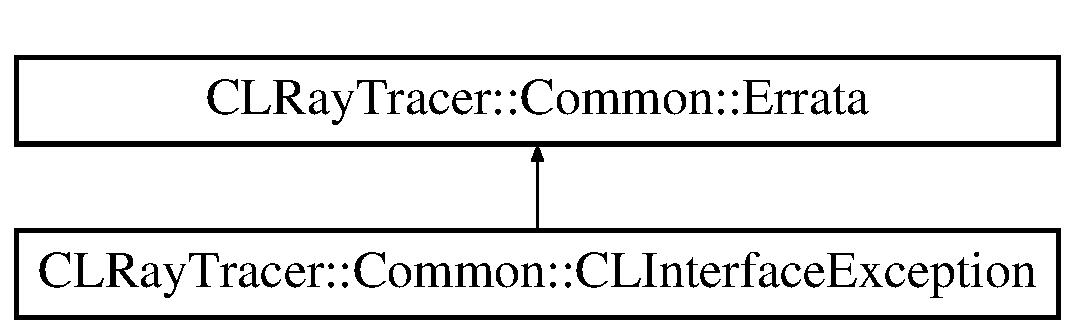
\includegraphics[height=2.000000cm]{class_c_l_ray_tracer_1_1_common_1_1_errata}
\end{center}
\end{figure}
\subsection*{Public Member Functions}
\begin{DoxyCompactItemize}
\item 
\hyperlink{class_c_l_ray_tracer_1_1_common_1_1_errata_a9b1f1e49c3415661fabd8aaa1cfd5534}{Errata} (const std\+::string \&error\+Message, const std\+::string \&\hyperlink{class_c_l_ray_tracer_1_1_common_1_1_errata_ab02c644698211e5b40a9eb8504c4ebfa}{file}, const std\+::string \&\hyperlink{class_c_l_ray_tracer_1_1_common_1_1_errata_ac591fef29757e5309cefa5f96e2f647f}{function}, int \hyperlink{class_c_l_ray_tracer_1_1_common_1_1_errata_ae53b458949d7a8b1438f72086dee9d6d}{line}, const std\+::exception $\ast$ex=N\+U\+LL)
\item 
\hyperlink{class_c_l_ray_tracer_1_1_common_1_1_errata_af49c6b9944517bc3ef964fb9ef71b8f8}{Errata} ()
\item 
std\+::string \hyperlink{class_c_l_ray_tracer_1_1_common_1_1_errata_ac2ea1fe3bebe8db7b6e0e0bf7ca68fb6}{message} () const 
\item 
std\+::string \hyperlink{class_c_l_ray_tracer_1_1_common_1_1_errata_ab02c644698211e5b40a9eb8504c4ebfa}{file} () const 
\item 
std\+::string \hyperlink{class_c_l_ray_tracer_1_1_common_1_1_errata_ac591fef29757e5309cefa5f96e2f647f}{function} () const 
\item 
int \hyperlink{class_c_l_ray_tracer_1_1_common_1_1_errata_ae53b458949d7a8b1438f72086dee9d6d}{line} () const 
\item 
const std\+::exception $\ast$ \hyperlink{class_c_l_ray_tracer_1_1_common_1_1_errata_a46e07afff80d38698637dff13edff67f}{exception} () const 
\end{DoxyCompactItemize}
\subsection*{Protected Attributes}
\begin{DoxyCompactItemize}
\item 
std\+::string {\bfseries \+\_\+message}\hypertarget{class_c_l_ray_tracer_1_1_common_1_1_errata_a7f0e72789382e50ca6e2d3ca4a2b8baf}{}\label{class_c_l_ray_tracer_1_1_common_1_1_errata_a7f0e72789382e50ca6e2d3ca4a2b8baf}

\item 
std\+::string {\bfseries \+\_\+file}\hypertarget{class_c_l_ray_tracer_1_1_common_1_1_errata_a242971b1502aff099c0e4d3b8fea0ea4}{}\label{class_c_l_ray_tracer_1_1_common_1_1_errata_a242971b1502aff099c0e4d3b8fea0ea4}

\item 
std\+::string {\bfseries \+\_\+function}\hypertarget{class_c_l_ray_tracer_1_1_common_1_1_errata_a7bda3dff0ec7f87a6ec98a02e245577e}{}\label{class_c_l_ray_tracer_1_1_common_1_1_errata_a7bda3dff0ec7f87a6ec98a02e245577e}

\item 
int {\bfseries \+\_\+line}\hypertarget{class_c_l_ray_tracer_1_1_common_1_1_errata_afdad0aa0eb34bc2d3ae5a091ddf941bd}{}\label{class_c_l_ray_tracer_1_1_common_1_1_errata_afdad0aa0eb34bc2d3ae5a091ddf941bd}

\item 
const std\+::exception $\ast$ {\bfseries \+\_\+exception}\hypertarget{class_c_l_ray_tracer_1_1_common_1_1_errata_aa0259f6c7a94ddd36ba05aec55ed04d4}{}\label{class_c_l_ray_tracer_1_1_common_1_1_errata_aa0259f6c7a94ddd36ba05aec55ed04d4}

\end{DoxyCompactItemize}
\subsection*{Friends}
\begin{DoxyCompactItemize}
\item 
std\+::ostream \& \hyperlink{class_c_l_ray_tracer_1_1_common_1_1_errata_a1b48ba32371d5121491672883a100d43}{operator$<$$<$} (std\+::ostream \&o, const \hyperlink{class_c_l_ray_tracer_1_1_common_1_1_errata}{Errata} \&err)
\end{DoxyCompactItemize}


\subsection{Detailed Description}
class \hyperlink{class_c_l_ray_tracer_1_1_common_1_1_errata}{Errata} contains error information 

\subsection{Constructor \& Destructor Documentation}
\index{C\+L\+Ray\+Tracer\+::\+Common\+::\+Errata@{C\+L\+Ray\+Tracer\+::\+Common\+::\+Errata}!Errata@{Errata}}
\index{Errata@{Errata}!C\+L\+Ray\+Tracer\+::\+Common\+::\+Errata@{C\+L\+Ray\+Tracer\+::\+Common\+::\+Errata}}
\subsubsection[{\texorpdfstring{Errata(const std\+::string \&error\+Message, const std\+::string \&file, const std\+::string \&function, int line, const std\+::exception $\ast$ex=\+N\+U\+L\+L)}{Errata(const std::string &errorMessage, const std::string &file, const std::string &function, int line, const std::exception *ex=NULL)}}]{\setlength{\rightskip}{0pt plus 5cm}C\+L\+Ray\+Tracer\+::\+Common\+::\+Errata\+::\+Errata (
\begin{DoxyParamCaption}
\item[{const std\+::string \&}]{error\+Message, }
\item[{const std\+::string \&}]{file, }
\item[{const std\+::string \&}]{function, }
\item[{int}]{line, }
\item[{const std\+::exception $\ast$}]{ex = {\ttfamily NULL}}
\end{DoxyParamCaption}
)\hspace{0.3cm}{\ttfamily [inline]}}\hypertarget{class_c_l_ray_tracer_1_1_common_1_1_errata_a9b1f1e49c3415661fabd8aaa1cfd5534}{}\label{class_c_l_ray_tracer_1_1_common_1_1_errata_a9b1f1e49c3415661fabd8aaa1cfd5534}
Constructor 
\begin{DoxyParams}{Parameters}
{\em error\+Message} & The error message \\
\hline
{\em file} & Code file name, in which the error had occurred \\
\hline
{\em function} & Function in which the error occurred \\
\hline
{\em line} & Line in which the error had occurred \\
\hline
{\em \mbox{[}optional\mbox{]}exception} & Exception that caused the error \\
\hline
\end{DoxyParams}
\index{C\+L\+Ray\+Tracer\+::\+Common\+::\+Errata@{C\+L\+Ray\+Tracer\+::\+Common\+::\+Errata}!Errata@{Errata}}
\index{Errata@{Errata}!C\+L\+Ray\+Tracer\+::\+Common\+::\+Errata@{C\+L\+Ray\+Tracer\+::\+Common\+::\+Errata}}
\subsubsection[{\texorpdfstring{Errata()}{Errata()}}]{\setlength{\rightskip}{0pt plus 5cm}C\+L\+Ray\+Tracer\+::\+Common\+::\+Errata\+::\+Errata (
\begin{DoxyParamCaption}
{}
\end{DoxyParamCaption}
)\hspace{0.3cm}{\ttfamily [inline]}}\hypertarget{class_c_l_ray_tracer_1_1_common_1_1_errata_af49c6b9944517bc3ef964fb9ef71b8f8}{}\label{class_c_l_ray_tracer_1_1_common_1_1_errata_af49c6b9944517bc3ef964fb9ef71b8f8}
Default constructor 

\subsection{Member Function Documentation}
\index{C\+L\+Ray\+Tracer\+::\+Common\+::\+Errata@{C\+L\+Ray\+Tracer\+::\+Common\+::\+Errata}!exception@{exception}}
\index{exception@{exception}!C\+L\+Ray\+Tracer\+::\+Common\+::\+Errata@{C\+L\+Ray\+Tracer\+::\+Common\+::\+Errata}}
\subsubsection[{\texorpdfstring{exception() const }{exception() const }}]{\setlength{\rightskip}{0pt plus 5cm}const std\+::exception$\ast$ C\+L\+Ray\+Tracer\+::\+Common\+::\+Errata\+::exception (
\begin{DoxyParamCaption}
{}
\end{DoxyParamCaption}
) const\hspace{0.3cm}{\ttfamily [inline]}}\hypertarget{class_c_l_ray_tracer_1_1_common_1_1_errata_a46e07afff80d38698637dff13edff67f}{}\label{class_c_l_ray_tracer_1_1_common_1_1_errata_a46e07afff80d38698637dff13edff67f}
Returns the exception object that caused the error \begin{DoxyReturn}{Returns}
Exception object that caused the error 
\end{DoxyReturn}
\index{C\+L\+Ray\+Tracer\+::\+Common\+::\+Errata@{C\+L\+Ray\+Tracer\+::\+Common\+::\+Errata}!file@{file}}
\index{file@{file}!C\+L\+Ray\+Tracer\+::\+Common\+::\+Errata@{C\+L\+Ray\+Tracer\+::\+Common\+::\+Errata}}
\subsubsection[{\texorpdfstring{file() const }{file() const }}]{\setlength{\rightskip}{0pt plus 5cm}std\+::string C\+L\+Ray\+Tracer\+::\+Common\+::\+Errata\+::file (
\begin{DoxyParamCaption}
{}
\end{DoxyParamCaption}
) const\hspace{0.3cm}{\ttfamily [inline]}}\hypertarget{class_c_l_ray_tracer_1_1_common_1_1_errata_ab02c644698211e5b40a9eb8504c4ebfa}{}\label{class_c_l_ray_tracer_1_1_common_1_1_errata_ab02c644698211e5b40a9eb8504c4ebfa}
Returns the code file name in which the error occurred \begin{DoxyReturn}{Returns}
Code file name in which the error occurred 
\end{DoxyReturn}
\index{C\+L\+Ray\+Tracer\+::\+Common\+::\+Errata@{C\+L\+Ray\+Tracer\+::\+Common\+::\+Errata}!function@{function}}
\index{function@{function}!C\+L\+Ray\+Tracer\+::\+Common\+::\+Errata@{C\+L\+Ray\+Tracer\+::\+Common\+::\+Errata}}
\subsubsection[{\texorpdfstring{function() const }{function() const }}]{\setlength{\rightskip}{0pt plus 5cm}std\+::string C\+L\+Ray\+Tracer\+::\+Common\+::\+Errata\+::function (
\begin{DoxyParamCaption}
{}
\end{DoxyParamCaption}
) const\hspace{0.3cm}{\ttfamily [inline]}}\hypertarget{class_c_l_ray_tracer_1_1_common_1_1_errata_ac591fef29757e5309cefa5f96e2f647f}{}\label{class_c_l_ray_tracer_1_1_common_1_1_errata_ac591fef29757e5309cefa5f96e2f647f}
Returns the function in which the error occurred \begin{DoxyReturn}{Returns}
Function in which the error occurred 
\end{DoxyReturn}
\index{C\+L\+Ray\+Tracer\+::\+Common\+::\+Errata@{C\+L\+Ray\+Tracer\+::\+Common\+::\+Errata}!line@{line}}
\index{line@{line}!C\+L\+Ray\+Tracer\+::\+Common\+::\+Errata@{C\+L\+Ray\+Tracer\+::\+Common\+::\+Errata}}
\subsubsection[{\texorpdfstring{line() const }{line() const }}]{\setlength{\rightskip}{0pt plus 5cm}int C\+L\+Ray\+Tracer\+::\+Common\+::\+Errata\+::line (
\begin{DoxyParamCaption}
{}
\end{DoxyParamCaption}
) const\hspace{0.3cm}{\ttfamily [inline]}}\hypertarget{class_c_l_ray_tracer_1_1_common_1_1_errata_ae53b458949d7a8b1438f72086dee9d6d}{}\label{class_c_l_ray_tracer_1_1_common_1_1_errata_ae53b458949d7a8b1438f72086dee9d6d}
Returns the line number in code file, where the error occurred \begin{DoxyReturn}{Returns}
Line number in code file, where the error occurred 
\end{DoxyReturn}
\index{C\+L\+Ray\+Tracer\+::\+Common\+::\+Errata@{C\+L\+Ray\+Tracer\+::\+Common\+::\+Errata}!message@{message}}
\index{message@{message}!C\+L\+Ray\+Tracer\+::\+Common\+::\+Errata@{C\+L\+Ray\+Tracer\+::\+Common\+::\+Errata}}
\subsubsection[{\texorpdfstring{message() const }{message() const }}]{\setlength{\rightskip}{0pt plus 5cm}std\+::string C\+L\+Ray\+Tracer\+::\+Common\+::\+Errata\+::message (
\begin{DoxyParamCaption}
{}
\end{DoxyParamCaption}
) const\hspace{0.3cm}{\ttfamily [inline]}}\hypertarget{class_c_l_ray_tracer_1_1_common_1_1_errata_ac2ea1fe3bebe8db7b6e0e0bf7ca68fb6}{}\label{class_c_l_ray_tracer_1_1_common_1_1_errata_ac2ea1fe3bebe8db7b6e0e0bf7ca68fb6}
Returns the error message \begin{DoxyReturn}{Returns}
Error message 
\end{DoxyReturn}


\subsection{Friends And Related Function Documentation}
\index{C\+L\+Ray\+Tracer\+::\+Common\+::\+Errata@{C\+L\+Ray\+Tracer\+::\+Common\+::\+Errata}!operator$<$$<$@{operator$<$$<$}}
\index{operator$<$$<$@{operator$<$$<$}!C\+L\+Ray\+Tracer\+::\+Common\+::\+Errata@{C\+L\+Ray\+Tracer\+::\+Common\+::\+Errata}}
\subsubsection[{\texorpdfstring{operator$<$$<$}{operator<<}}]{\setlength{\rightskip}{0pt plus 5cm}std\+::ostream\& operator$<$$<$ (
\begin{DoxyParamCaption}
\item[{std\+::ostream \&}]{o, }
\item[{const {\bf Errata} \&}]{err}
\end{DoxyParamCaption}
)\hspace{0.3cm}{\ttfamily [friend]}}\hypertarget{class_c_l_ray_tracer_1_1_common_1_1_errata_a1b48ba32371d5121491672883a100d43}{}\label{class_c_l_ray_tracer_1_1_common_1_1_errata_a1b48ba32371d5121491672883a100d43}
Allows easy output of \hyperlink{class_c_l_ray_tracer_1_1_common_1_1_errata}{Errata} object

Operator for easy output of error objects 

The documentation for this class was generated from the following file\+:\begin{DoxyCompactItemize}
\item 
Include/\+Common/\hyperlink{_errata_8h}{Errata.\+h}\end{DoxyCompactItemize}

\hypertarget{class_c_l_ray_tracer_1_1_open_c_l_utils_1_1_c_l_device_1_1_execution_info}{}\section{C\+L\+Ray\+Tracer\+:\+:Open\+C\+L\+Utils\+:\+:C\+L\+Device\+:\+:Execution\+Info Class Reference}
\label{class_c_l_ray_tracer_1_1_open_c_l_utils_1_1_c_l_device_1_1_execution_info}\index{C\+L\+Ray\+Tracer\+::\+Open\+C\+L\+Utils\+::\+C\+L\+Device\+::\+Execution\+Info@{C\+L\+Ray\+Tracer\+::\+Open\+C\+L\+Utils\+::\+C\+L\+Device\+::\+Execution\+Info}}


{\ttfamily \#include $<$C\+L\+Interface.\+h$>$}

\subsection*{Public Member Functions}
\begin{DoxyCompactItemize}
\item 
\hyperlink{class_c_l_ray_tracer_1_1_open_c_l_utils_1_1_c_l_device_1_1_execution_info_a8b180abf92896a1d249b9596881a97b9}{Execution\+Info} (cl\+\_\+device\+\_\+id device\+Id)
\item 
\hyperlink{class_c_l_ray_tracer_1_1_open_c_l_utils_1_1_c_l_device_1_1_execution_info_a4151b2470b4e44ce9c2526c2c3a94f95}{D\+E\+V\+I\+C\+E\+\_\+\+P\+R\+O\+P\+E\+R\+T\+Y\+\_\+\+G\+E\+T\+T\+ER} (get\+Max\+Parameter\+Size, C\+L\+\_\+\+D\+E\+V\+I\+C\+E\+\_\+\+M\+A\+X\+\_\+\+P\+A\+R\+A\+M\+E\+T\+E\+R\+\_\+\+S\+I\+ZE, size\+\_\+t)
\item 
\hyperlink{class_c_l_ray_tracer_1_1_open_c_l_utils_1_1_c_l_device_1_1_execution_info_a61ccac3726f090580c18895ec508c499}{D\+E\+V\+I\+C\+E\+\_\+\+P\+R\+O\+P\+E\+R\+T\+Y\+\_\+\+G\+E\+T\+T\+ER} (get\+Profiling\+Timer\+Resolution, C\+L\+\_\+\+D\+E\+V\+I\+C\+E\+\_\+\+P\+R\+O\+F\+I\+L\+I\+N\+G\+\_\+\+T\+I\+M\+E\+R\+\_\+\+R\+E\+S\+O\+L\+U\+T\+I\+ON, size\+\_\+t)
\item 
\hyperlink{class_c_l_ray_tracer_1_1_open_c_l_utils_1_1_c_l_device_1_1_execution_info_af68dd449ebc085c4ecfc3d51a7f6ef63}{D\+E\+V\+I\+C\+E\+\_\+\+P\+R\+O\+P\+E\+R\+T\+Y\+\_\+\+G\+E\+T\+T\+ER} (get\+Max\+Clock\+Frequency, C\+L\+\_\+\+D\+E\+V\+I\+C\+E\+\_\+\+M\+A\+X\+\_\+\+C\+L\+O\+C\+K\+\_\+\+F\+R\+E\+Q\+U\+E\+N\+CY, cl\+\_\+uint)
\item 
\hyperlink{class_c_l_ray_tracer_1_1_open_c_l_utils_1_1_c_l_device_1_1_execution_info_ab43b721775b5e30d81c6d74981b7379a}{D\+E\+V\+I\+C\+E\+\_\+\+P\+R\+O\+P\+E\+R\+T\+Y\+\_\+\+G\+E\+T\+T\+ER} (get\+Max\+Compute\+Units, C\+L\+\_\+\+D\+E\+V\+I\+C\+E\+\_\+\+M\+A\+X\+\_\+\+C\+O\+M\+P\+U\+T\+E\+\_\+\+U\+N\+I\+TS, cl\+\_\+uint)
\item 
\hyperlink{class_c_l_ray_tracer_1_1_open_c_l_utils_1_1_c_l_device_1_1_execution_info_a4488367d64bd92f4057e270bfaac0b6c}{D\+E\+V\+I\+C\+E\+\_\+\+P\+R\+O\+P\+E\+R\+T\+Y\+\_\+\+G\+E\+T\+T\+ER} (get\+Max\+Constant\+Args, C\+L\+\_\+\+D\+E\+V\+I\+C\+E\+\_\+\+M\+A\+X\+\_\+\+C\+O\+N\+S\+T\+A\+N\+T\+\_\+\+A\+R\+GS, cl\+\_\+uint)
\item 
\hyperlink{class_c_l_ray_tracer_1_1_open_c_l_utils_1_1_c_l_device_1_1_execution_info_aa7faa21a7c6595c17b41e4ac4d55d1b4}{D\+E\+V\+I\+C\+E\+\_\+\+P\+R\+O\+P\+E\+R\+T\+Y\+\_\+\+G\+E\+T\+T\+ER} (get\+Mem\+Base\+Addr\+Align, C\+L\+\_\+\+D\+E\+V\+I\+C\+E\+\_\+\+M\+E\+M\+\_\+\+B\+A\+S\+E\+\_\+\+A\+D\+D\+R\+\_\+\+A\+L\+I\+GN, cl\+\_\+uint)
\item 
\hyperlink{class_c_l_ray_tracer_1_1_open_c_l_utils_1_1_c_l_device_1_1_execution_info_a791fd2f611c60d4b1640c6b60cc22bdf}{D\+E\+V\+I\+C\+E\+\_\+\+P\+R\+O\+P\+E\+R\+T\+Y\+\_\+\+G\+E\+T\+T\+ER} (get\+Min\+Data\+Type\+Align\+Size, C\+L\+\_\+\+D\+E\+V\+I\+C\+E\+\_\+\+M\+I\+N\+\_\+\+D\+A\+T\+A\+\_\+\+T\+Y\+P\+E\+\_\+\+A\+L\+I\+G\+N\+\_\+\+S\+I\+ZE, cl\+\_\+uint)
\item 
\hyperlink{class_c_l_ray_tracer_1_1_open_c_l_utils_1_1_c_l_device_1_1_execution_info_ab57138db2a1e4f56187549f8f569974a}{D\+E\+V\+I\+C\+E\+\_\+\+P\+R\+O\+P\+E\+R\+T\+Y\+\_\+\+G\+E\+T\+T\+ER} (get\+Max\+Constant\+Buffer\+Size, C\+L\+\_\+\+D\+E\+V\+I\+C\+E\+\_\+\+M\+A\+X\+\_\+\+C\+O\+N\+S\+T\+A\+N\+T\+\_\+\+B\+U\+F\+F\+E\+R\+\_\+\+S\+I\+ZE, cl\+\_\+ulong)
\item 
\hyperlink{class_c_l_ray_tracer_1_1_open_c_l_utils_1_1_c_l_device_1_1_execution_info_a6169e3e4eb0af6d68f6b09999aadc33e}{D\+E\+V\+I\+C\+E\+\_\+\+P\+R\+O\+P\+E\+R\+T\+Y\+\_\+\+G\+E\+T\+T\+ER} (get\+Device\+Queue\+Properties, C\+L\+\_\+\+D\+E\+V\+I\+C\+E\+\_\+\+Q\+U\+E\+U\+E\+\_\+\+P\+R\+O\+P\+E\+R\+T\+I\+ES, cl\+\_\+command\+\_\+queue\+\_\+properties)
\end{DoxyCompactItemize}


\subsection{Detailed Description}
Class \hyperlink{class_c_l_ray_tracer_1_1_open_c_l_utils_1_1_c_l_device_1_1_execution_info}{Execution\+Info} groups device properties related to kernel execution 

\subsection{Constructor \& Destructor Documentation}
\index{C\+L\+Ray\+Tracer\+::\+Open\+C\+L\+Utils\+::\+C\+L\+Device\+::\+Execution\+Info@{C\+L\+Ray\+Tracer\+::\+Open\+C\+L\+Utils\+::\+C\+L\+Device\+::\+Execution\+Info}!Execution\+Info@{Execution\+Info}}
\index{Execution\+Info@{Execution\+Info}!C\+L\+Ray\+Tracer\+::\+Open\+C\+L\+Utils\+::\+C\+L\+Device\+::\+Execution\+Info@{C\+L\+Ray\+Tracer\+::\+Open\+C\+L\+Utils\+::\+C\+L\+Device\+::\+Execution\+Info}}
\subsubsection[{\texorpdfstring{Execution\+Info(cl\+\_\+device\+\_\+id device\+Id)}{ExecutionInfo(cl_device_id deviceId)}}]{\setlength{\rightskip}{0pt plus 5cm}C\+L\+Ray\+Tracer\+::\+Open\+C\+L\+Utils\+::\+C\+L\+Device\+::\+Execution\+Info\+::\+Execution\+Info (
\begin{DoxyParamCaption}
\item[{cl\+\_\+device\+\_\+id}]{device\+Id}
\end{DoxyParamCaption}
)\hspace{0.3cm}{\ttfamily [inline]}}\hypertarget{class_c_l_ray_tracer_1_1_open_c_l_utils_1_1_c_l_device_1_1_execution_info_a8b180abf92896a1d249b9596881a97b9}{}\label{class_c_l_ray_tracer_1_1_open_c_l_utils_1_1_c_l_device_1_1_execution_info_a8b180abf92896a1d249b9596881a97b9}
Constructor 

\subsection{Member Function Documentation}
\index{C\+L\+Ray\+Tracer\+::\+Open\+C\+L\+Utils\+::\+C\+L\+Device\+::\+Execution\+Info@{C\+L\+Ray\+Tracer\+::\+Open\+C\+L\+Utils\+::\+C\+L\+Device\+::\+Execution\+Info}!D\+E\+V\+I\+C\+E\+\_\+\+P\+R\+O\+P\+E\+R\+T\+Y\+\_\+\+G\+E\+T\+T\+ER@{D\+E\+V\+I\+C\+E\+\_\+\+P\+R\+O\+P\+E\+R\+T\+Y\+\_\+\+G\+E\+T\+T\+ER}}
\index{D\+E\+V\+I\+C\+E\+\_\+\+P\+R\+O\+P\+E\+R\+T\+Y\+\_\+\+G\+E\+T\+T\+ER@{D\+E\+V\+I\+C\+E\+\_\+\+P\+R\+O\+P\+E\+R\+T\+Y\+\_\+\+G\+E\+T\+T\+ER}!C\+L\+Ray\+Tracer\+::\+Open\+C\+L\+Utils\+::\+C\+L\+Device\+::\+Execution\+Info@{C\+L\+Ray\+Tracer\+::\+Open\+C\+L\+Utils\+::\+C\+L\+Device\+::\+Execution\+Info}}
\subsubsection[{\texorpdfstring{D\+E\+V\+I\+C\+E\+\_\+\+P\+R\+O\+P\+E\+R\+T\+Y\+\_\+\+G\+E\+T\+T\+E\+R(get\+Max\+Parameter\+Size, C\+L\+\_\+\+D\+E\+V\+I\+C\+E\+\_\+\+M\+A\+X\+\_\+\+P\+A\+R\+A\+M\+E\+T\+E\+R\+\_\+\+S\+I\+Z\+E, size\+\_\+t)}{DEVICE_PROPERTY_GETTER(getMaxParameterSize, CL_DEVICE_MAX_PARAMETER_SIZE, size_t)}}]{\setlength{\rightskip}{0pt plus 5cm}C\+L\+Ray\+Tracer\+::\+Open\+C\+L\+Utils\+::\+C\+L\+Device\+::\+Execution\+Info\+::\+D\+E\+V\+I\+C\+E\+\_\+\+P\+R\+O\+P\+E\+R\+T\+Y\+\_\+\+G\+E\+T\+T\+ER (
\begin{DoxyParamCaption}
\item[{get\+Max\+Parameter\+Size}]{, }
\item[{C\+L\+\_\+\+D\+E\+V\+I\+C\+E\+\_\+\+M\+A\+X\+\_\+\+P\+A\+R\+A\+M\+E\+T\+E\+R\+\_\+\+S\+I\+ZE}]{, }
\item[{size\+\_\+t}]{}
\end{DoxyParamCaption}
)}\hypertarget{class_c_l_ray_tracer_1_1_open_c_l_utils_1_1_c_l_device_1_1_execution_info_a4151b2470b4e44ce9c2526c2c3a94f95}{}\label{class_c_l_ray_tracer_1_1_open_c_l_utils_1_1_c_l_device_1_1_execution_info_a4151b2470b4e44ce9c2526c2c3a94f95}
Retrieves property of Open\+CL Device\+: Max size in bytes of the arguments that can be passed to a kernel 
\begin{DoxyParams}[1]{Parameters}
\mbox{\tt out}  & {\em } & \\
\hline
\end{DoxyParams}
\index{C\+L\+Ray\+Tracer\+::\+Open\+C\+L\+Utils\+::\+C\+L\+Device\+::\+Execution\+Info@{C\+L\+Ray\+Tracer\+::\+Open\+C\+L\+Utils\+::\+C\+L\+Device\+::\+Execution\+Info}!D\+E\+V\+I\+C\+E\+\_\+\+P\+R\+O\+P\+E\+R\+T\+Y\+\_\+\+G\+E\+T\+T\+ER@{D\+E\+V\+I\+C\+E\+\_\+\+P\+R\+O\+P\+E\+R\+T\+Y\+\_\+\+G\+E\+T\+T\+ER}}
\index{D\+E\+V\+I\+C\+E\+\_\+\+P\+R\+O\+P\+E\+R\+T\+Y\+\_\+\+G\+E\+T\+T\+ER@{D\+E\+V\+I\+C\+E\+\_\+\+P\+R\+O\+P\+E\+R\+T\+Y\+\_\+\+G\+E\+T\+T\+ER}!C\+L\+Ray\+Tracer\+::\+Open\+C\+L\+Utils\+::\+C\+L\+Device\+::\+Execution\+Info@{C\+L\+Ray\+Tracer\+::\+Open\+C\+L\+Utils\+::\+C\+L\+Device\+::\+Execution\+Info}}
\subsubsection[{\texorpdfstring{D\+E\+V\+I\+C\+E\+\_\+\+P\+R\+O\+P\+E\+R\+T\+Y\+\_\+\+G\+E\+T\+T\+E\+R(get\+Profiling\+Timer\+Resolution, C\+L\+\_\+\+D\+E\+V\+I\+C\+E\+\_\+\+P\+R\+O\+F\+I\+L\+I\+N\+G\+\_\+\+T\+I\+M\+E\+R\+\_\+\+R\+E\+S\+O\+L\+U\+T\+I\+O\+N, size\+\_\+t)}{DEVICE_PROPERTY_GETTER(getProfilingTimerResolution, CL_DEVICE_PROFILING_TIMER_RESOLUTION, size_t)}}]{\setlength{\rightskip}{0pt plus 5cm}C\+L\+Ray\+Tracer\+::\+Open\+C\+L\+Utils\+::\+C\+L\+Device\+::\+Execution\+Info\+::\+D\+E\+V\+I\+C\+E\+\_\+\+P\+R\+O\+P\+E\+R\+T\+Y\+\_\+\+G\+E\+T\+T\+ER (
\begin{DoxyParamCaption}
\item[{get\+Profiling\+Timer\+Resolution}]{, }
\item[{C\+L\+\_\+\+D\+E\+V\+I\+C\+E\+\_\+\+P\+R\+O\+F\+I\+L\+I\+N\+G\+\_\+\+T\+I\+M\+E\+R\+\_\+\+R\+E\+S\+O\+L\+U\+T\+I\+ON}]{, }
\item[{size\+\_\+t}]{}
\end{DoxyParamCaption}
)}\hypertarget{class_c_l_ray_tracer_1_1_open_c_l_utils_1_1_c_l_device_1_1_execution_info_a61ccac3726f090580c18895ec508c499}{}\label{class_c_l_ray_tracer_1_1_open_c_l_utils_1_1_c_l_device_1_1_execution_info_a61ccac3726f090580c18895ec508c499}
Retrieves property of Open\+CL Device\+: Resolution of device timer in nanoseconds 
\begin{DoxyParams}[1]{Parameters}
\mbox{\tt out}  & {\em } & \\
\hline
\end{DoxyParams}
\index{C\+L\+Ray\+Tracer\+::\+Open\+C\+L\+Utils\+::\+C\+L\+Device\+::\+Execution\+Info@{C\+L\+Ray\+Tracer\+::\+Open\+C\+L\+Utils\+::\+C\+L\+Device\+::\+Execution\+Info}!D\+E\+V\+I\+C\+E\+\_\+\+P\+R\+O\+P\+E\+R\+T\+Y\+\_\+\+G\+E\+T\+T\+ER@{D\+E\+V\+I\+C\+E\+\_\+\+P\+R\+O\+P\+E\+R\+T\+Y\+\_\+\+G\+E\+T\+T\+ER}}
\index{D\+E\+V\+I\+C\+E\+\_\+\+P\+R\+O\+P\+E\+R\+T\+Y\+\_\+\+G\+E\+T\+T\+ER@{D\+E\+V\+I\+C\+E\+\_\+\+P\+R\+O\+P\+E\+R\+T\+Y\+\_\+\+G\+E\+T\+T\+ER}!C\+L\+Ray\+Tracer\+::\+Open\+C\+L\+Utils\+::\+C\+L\+Device\+::\+Execution\+Info@{C\+L\+Ray\+Tracer\+::\+Open\+C\+L\+Utils\+::\+C\+L\+Device\+::\+Execution\+Info}}
\subsubsection[{\texorpdfstring{D\+E\+V\+I\+C\+E\+\_\+\+P\+R\+O\+P\+E\+R\+T\+Y\+\_\+\+G\+E\+T\+T\+E\+R(get\+Max\+Clock\+Frequency, C\+L\+\_\+\+D\+E\+V\+I\+C\+E\+\_\+\+M\+A\+X\+\_\+\+C\+L\+O\+C\+K\+\_\+\+F\+R\+E\+Q\+U\+E\+N\+C\+Y, cl\+\_\+uint)}{DEVICE_PROPERTY_GETTER(getMaxClockFrequency, CL_DEVICE_MAX_CLOCK_FREQUENCY, cl_uint)}}]{\setlength{\rightskip}{0pt plus 5cm}C\+L\+Ray\+Tracer\+::\+Open\+C\+L\+Utils\+::\+C\+L\+Device\+::\+Execution\+Info\+::\+D\+E\+V\+I\+C\+E\+\_\+\+P\+R\+O\+P\+E\+R\+T\+Y\+\_\+\+G\+E\+T\+T\+ER (
\begin{DoxyParamCaption}
\item[{get\+Max\+Clock\+Frequency}]{, }
\item[{C\+L\+\_\+\+D\+E\+V\+I\+C\+E\+\_\+\+M\+A\+X\+\_\+\+C\+L\+O\+C\+K\+\_\+\+F\+R\+E\+Q\+U\+E\+N\+CY}]{, }
\item[{cl\+\_\+uint}]{}
\end{DoxyParamCaption}
)}\hypertarget{class_c_l_ray_tracer_1_1_open_c_l_utils_1_1_c_l_device_1_1_execution_info_af68dd449ebc085c4ecfc3d51a7f6ef63}{}\label{class_c_l_ray_tracer_1_1_open_c_l_utils_1_1_c_l_device_1_1_execution_info_af68dd449ebc085c4ecfc3d51a7f6ef63}
Retrieves property of Open\+CL Device\+: Maximum configured clock frequency of the device in M\+Hz. 
\begin{DoxyParams}[1]{Parameters}
\mbox{\tt out}  & {\em } & \\
\hline
\end{DoxyParams}
\index{C\+L\+Ray\+Tracer\+::\+Open\+C\+L\+Utils\+::\+C\+L\+Device\+::\+Execution\+Info@{C\+L\+Ray\+Tracer\+::\+Open\+C\+L\+Utils\+::\+C\+L\+Device\+::\+Execution\+Info}!D\+E\+V\+I\+C\+E\+\_\+\+P\+R\+O\+P\+E\+R\+T\+Y\+\_\+\+G\+E\+T\+T\+ER@{D\+E\+V\+I\+C\+E\+\_\+\+P\+R\+O\+P\+E\+R\+T\+Y\+\_\+\+G\+E\+T\+T\+ER}}
\index{D\+E\+V\+I\+C\+E\+\_\+\+P\+R\+O\+P\+E\+R\+T\+Y\+\_\+\+G\+E\+T\+T\+ER@{D\+E\+V\+I\+C\+E\+\_\+\+P\+R\+O\+P\+E\+R\+T\+Y\+\_\+\+G\+E\+T\+T\+ER}!C\+L\+Ray\+Tracer\+::\+Open\+C\+L\+Utils\+::\+C\+L\+Device\+::\+Execution\+Info@{C\+L\+Ray\+Tracer\+::\+Open\+C\+L\+Utils\+::\+C\+L\+Device\+::\+Execution\+Info}}
\subsubsection[{\texorpdfstring{D\+E\+V\+I\+C\+E\+\_\+\+P\+R\+O\+P\+E\+R\+T\+Y\+\_\+\+G\+E\+T\+T\+E\+R(get\+Max\+Compute\+Units, C\+L\+\_\+\+D\+E\+V\+I\+C\+E\+\_\+\+M\+A\+X\+\_\+\+C\+O\+M\+P\+U\+T\+E\+\_\+\+U\+N\+I\+T\+S, cl\+\_\+uint)}{DEVICE_PROPERTY_GETTER(getMaxComputeUnits, CL_DEVICE_MAX_COMPUTE_UNITS, cl_uint)}}]{\setlength{\rightskip}{0pt plus 5cm}C\+L\+Ray\+Tracer\+::\+Open\+C\+L\+Utils\+::\+C\+L\+Device\+::\+Execution\+Info\+::\+D\+E\+V\+I\+C\+E\+\_\+\+P\+R\+O\+P\+E\+R\+T\+Y\+\_\+\+G\+E\+T\+T\+ER (
\begin{DoxyParamCaption}
\item[{get\+Max\+Compute\+Units}]{, }
\item[{C\+L\+\_\+\+D\+E\+V\+I\+C\+E\+\_\+\+M\+A\+X\+\_\+\+C\+O\+M\+P\+U\+T\+E\+\_\+\+U\+N\+I\+TS}]{, }
\item[{cl\+\_\+uint}]{}
\end{DoxyParamCaption}
)}\hypertarget{class_c_l_ray_tracer_1_1_open_c_l_utils_1_1_c_l_device_1_1_execution_info_ab43b721775b5e30d81c6d74981b7379a}{}\label{class_c_l_ray_tracer_1_1_open_c_l_utils_1_1_c_l_device_1_1_execution_info_ab43b721775b5e30d81c6d74981b7379a}
Retrieves property of Open\+CL Device\+: The number of parallel compute cores on the Open\+CL device. 
\begin{DoxyParams}[1]{Parameters}
\mbox{\tt out}  & {\em } & \\
\hline
\end{DoxyParams}
\index{C\+L\+Ray\+Tracer\+::\+Open\+C\+L\+Utils\+::\+C\+L\+Device\+::\+Execution\+Info@{C\+L\+Ray\+Tracer\+::\+Open\+C\+L\+Utils\+::\+C\+L\+Device\+::\+Execution\+Info}!D\+E\+V\+I\+C\+E\+\_\+\+P\+R\+O\+P\+E\+R\+T\+Y\+\_\+\+G\+E\+T\+T\+ER@{D\+E\+V\+I\+C\+E\+\_\+\+P\+R\+O\+P\+E\+R\+T\+Y\+\_\+\+G\+E\+T\+T\+ER}}
\index{D\+E\+V\+I\+C\+E\+\_\+\+P\+R\+O\+P\+E\+R\+T\+Y\+\_\+\+G\+E\+T\+T\+ER@{D\+E\+V\+I\+C\+E\+\_\+\+P\+R\+O\+P\+E\+R\+T\+Y\+\_\+\+G\+E\+T\+T\+ER}!C\+L\+Ray\+Tracer\+::\+Open\+C\+L\+Utils\+::\+C\+L\+Device\+::\+Execution\+Info@{C\+L\+Ray\+Tracer\+::\+Open\+C\+L\+Utils\+::\+C\+L\+Device\+::\+Execution\+Info}}
\subsubsection[{\texorpdfstring{D\+E\+V\+I\+C\+E\+\_\+\+P\+R\+O\+P\+E\+R\+T\+Y\+\_\+\+G\+E\+T\+T\+E\+R(get\+Max\+Constant\+Args, C\+L\+\_\+\+D\+E\+V\+I\+C\+E\+\_\+\+M\+A\+X\+\_\+\+C\+O\+N\+S\+T\+A\+N\+T\+\_\+\+A\+R\+G\+S, cl\+\_\+uint)}{DEVICE_PROPERTY_GETTER(getMaxConstantArgs, CL_DEVICE_MAX_CONSTANT_ARGS, cl_uint)}}]{\setlength{\rightskip}{0pt plus 5cm}C\+L\+Ray\+Tracer\+::\+Open\+C\+L\+Utils\+::\+C\+L\+Device\+::\+Execution\+Info\+::\+D\+E\+V\+I\+C\+E\+\_\+\+P\+R\+O\+P\+E\+R\+T\+Y\+\_\+\+G\+E\+T\+T\+ER (
\begin{DoxyParamCaption}
\item[{get\+Max\+Constant\+Args}]{, }
\item[{C\+L\+\_\+\+D\+E\+V\+I\+C\+E\+\_\+\+M\+A\+X\+\_\+\+C\+O\+N\+S\+T\+A\+N\+T\+\_\+\+A\+R\+GS}]{, }
\item[{cl\+\_\+uint}]{}
\end{DoxyParamCaption}
)}\hypertarget{class_c_l_ray_tracer_1_1_open_c_l_utils_1_1_c_l_device_1_1_execution_info_a4488367d64bd92f4057e270bfaac0b6c}{}\label{class_c_l_ray_tracer_1_1_open_c_l_utils_1_1_c_l_device_1_1_execution_info_a4488367d64bd92f4057e270bfaac0b6c}
Retrieves property of Open\+CL Device\+: Max number of arguments declared with the \+\_\+\+\_\+constant qualifier in a kernel 
\begin{DoxyParams}[1]{Parameters}
\mbox{\tt out}  & {\em } & \\
\hline
\end{DoxyParams}
\index{C\+L\+Ray\+Tracer\+::\+Open\+C\+L\+Utils\+::\+C\+L\+Device\+::\+Execution\+Info@{C\+L\+Ray\+Tracer\+::\+Open\+C\+L\+Utils\+::\+C\+L\+Device\+::\+Execution\+Info}!D\+E\+V\+I\+C\+E\+\_\+\+P\+R\+O\+P\+E\+R\+T\+Y\+\_\+\+G\+E\+T\+T\+ER@{D\+E\+V\+I\+C\+E\+\_\+\+P\+R\+O\+P\+E\+R\+T\+Y\+\_\+\+G\+E\+T\+T\+ER}}
\index{D\+E\+V\+I\+C\+E\+\_\+\+P\+R\+O\+P\+E\+R\+T\+Y\+\_\+\+G\+E\+T\+T\+ER@{D\+E\+V\+I\+C\+E\+\_\+\+P\+R\+O\+P\+E\+R\+T\+Y\+\_\+\+G\+E\+T\+T\+ER}!C\+L\+Ray\+Tracer\+::\+Open\+C\+L\+Utils\+::\+C\+L\+Device\+::\+Execution\+Info@{C\+L\+Ray\+Tracer\+::\+Open\+C\+L\+Utils\+::\+C\+L\+Device\+::\+Execution\+Info}}
\subsubsection[{\texorpdfstring{D\+E\+V\+I\+C\+E\+\_\+\+P\+R\+O\+P\+E\+R\+T\+Y\+\_\+\+G\+E\+T\+T\+E\+R(get\+Mem\+Base\+Addr\+Align, C\+L\+\_\+\+D\+E\+V\+I\+C\+E\+\_\+\+M\+E\+M\+\_\+\+B\+A\+S\+E\+\_\+\+A\+D\+D\+R\+\_\+\+A\+L\+I\+G\+N, cl\+\_\+uint)}{DEVICE_PROPERTY_GETTER(getMemBaseAddrAlign, CL_DEVICE_MEM_BASE_ADDR_ALIGN, cl_uint)}}]{\setlength{\rightskip}{0pt plus 5cm}C\+L\+Ray\+Tracer\+::\+Open\+C\+L\+Utils\+::\+C\+L\+Device\+::\+Execution\+Info\+::\+D\+E\+V\+I\+C\+E\+\_\+\+P\+R\+O\+P\+E\+R\+T\+Y\+\_\+\+G\+E\+T\+T\+ER (
\begin{DoxyParamCaption}
\item[{get\+Mem\+Base\+Addr\+Align}]{, }
\item[{C\+L\+\_\+\+D\+E\+V\+I\+C\+E\+\_\+\+M\+E\+M\+\_\+\+B\+A\+S\+E\+\_\+\+A\+D\+D\+R\+\_\+\+A\+L\+I\+GN}]{, }
\item[{cl\+\_\+uint}]{}
\end{DoxyParamCaption}
)}\hypertarget{class_c_l_ray_tracer_1_1_open_c_l_utils_1_1_c_l_device_1_1_execution_info_aa7faa21a7c6595c17b41e4ac4d55d1b4}{}\label{class_c_l_ray_tracer_1_1_open_c_l_utils_1_1_c_l_device_1_1_execution_info_aa7faa21a7c6595c17b41e4ac4d55d1b4}
Retrieves property of Open\+CL Device\+: Describes the alignment in bits of the base address of any allocated memory object. 
\begin{DoxyParams}[1]{Parameters}
\mbox{\tt out}  & {\em } & \\
\hline
\end{DoxyParams}
\index{C\+L\+Ray\+Tracer\+::\+Open\+C\+L\+Utils\+::\+C\+L\+Device\+::\+Execution\+Info@{C\+L\+Ray\+Tracer\+::\+Open\+C\+L\+Utils\+::\+C\+L\+Device\+::\+Execution\+Info}!D\+E\+V\+I\+C\+E\+\_\+\+P\+R\+O\+P\+E\+R\+T\+Y\+\_\+\+G\+E\+T\+T\+ER@{D\+E\+V\+I\+C\+E\+\_\+\+P\+R\+O\+P\+E\+R\+T\+Y\+\_\+\+G\+E\+T\+T\+ER}}
\index{D\+E\+V\+I\+C\+E\+\_\+\+P\+R\+O\+P\+E\+R\+T\+Y\+\_\+\+G\+E\+T\+T\+ER@{D\+E\+V\+I\+C\+E\+\_\+\+P\+R\+O\+P\+E\+R\+T\+Y\+\_\+\+G\+E\+T\+T\+ER}!C\+L\+Ray\+Tracer\+::\+Open\+C\+L\+Utils\+::\+C\+L\+Device\+::\+Execution\+Info@{C\+L\+Ray\+Tracer\+::\+Open\+C\+L\+Utils\+::\+C\+L\+Device\+::\+Execution\+Info}}
\subsubsection[{\texorpdfstring{D\+E\+V\+I\+C\+E\+\_\+\+P\+R\+O\+P\+E\+R\+T\+Y\+\_\+\+G\+E\+T\+T\+E\+R(get\+Min\+Data\+Type\+Align\+Size, C\+L\+\_\+\+D\+E\+V\+I\+C\+E\+\_\+\+M\+I\+N\+\_\+\+D\+A\+T\+A\+\_\+\+T\+Y\+P\+E\+\_\+\+A\+L\+I\+G\+N\+\_\+\+S\+I\+Z\+E, cl\+\_\+uint)}{DEVICE_PROPERTY_GETTER(getMinDataTypeAlignSize, CL_DEVICE_MIN_DATA_TYPE_ALIGN_SIZE, cl_uint)}}]{\setlength{\rightskip}{0pt plus 5cm}C\+L\+Ray\+Tracer\+::\+Open\+C\+L\+Utils\+::\+C\+L\+Device\+::\+Execution\+Info\+::\+D\+E\+V\+I\+C\+E\+\_\+\+P\+R\+O\+P\+E\+R\+T\+Y\+\_\+\+G\+E\+T\+T\+ER (
\begin{DoxyParamCaption}
\item[{get\+Min\+Data\+Type\+Align\+Size}]{, }
\item[{C\+L\+\_\+\+D\+E\+V\+I\+C\+E\+\_\+\+M\+I\+N\+\_\+\+D\+A\+T\+A\+\_\+\+T\+Y\+P\+E\+\_\+\+A\+L\+I\+G\+N\+\_\+\+S\+I\+ZE}]{, }
\item[{cl\+\_\+uint}]{}
\end{DoxyParamCaption}
)}\hypertarget{class_c_l_ray_tracer_1_1_open_c_l_utils_1_1_c_l_device_1_1_execution_info_a791fd2f611c60d4b1640c6b60cc22bdf}{}\label{class_c_l_ray_tracer_1_1_open_c_l_utils_1_1_c_l_device_1_1_execution_info_a791fd2f611c60d4b1640c6b60cc22bdf}
Retrieves property of Open\+CL Device\+: The smallest alignment in bytes which can be used for any data type 
\begin{DoxyParams}[1]{Parameters}
\mbox{\tt out}  & {\em } & \\
\hline
\end{DoxyParams}
\index{C\+L\+Ray\+Tracer\+::\+Open\+C\+L\+Utils\+::\+C\+L\+Device\+::\+Execution\+Info@{C\+L\+Ray\+Tracer\+::\+Open\+C\+L\+Utils\+::\+C\+L\+Device\+::\+Execution\+Info}!D\+E\+V\+I\+C\+E\+\_\+\+P\+R\+O\+P\+E\+R\+T\+Y\+\_\+\+G\+E\+T\+T\+ER@{D\+E\+V\+I\+C\+E\+\_\+\+P\+R\+O\+P\+E\+R\+T\+Y\+\_\+\+G\+E\+T\+T\+ER}}
\index{D\+E\+V\+I\+C\+E\+\_\+\+P\+R\+O\+P\+E\+R\+T\+Y\+\_\+\+G\+E\+T\+T\+ER@{D\+E\+V\+I\+C\+E\+\_\+\+P\+R\+O\+P\+E\+R\+T\+Y\+\_\+\+G\+E\+T\+T\+ER}!C\+L\+Ray\+Tracer\+::\+Open\+C\+L\+Utils\+::\+C\+L\+Device\+::\+Execution\+Info@{C\+L\+Ray\+Tracer\+::\+Open\+C\+L\+Utils\+::\+C\+L\+Device\+::\+Execution\+Info}}
\subsubsection[{\texorpdfstring{D\+E\+V\+I\+C\+E\+\_\+\+P\+R\+O\+P\+E\+R\+T\+Y\+\_\+\+G\+E\+T\+T\+E\+R(get\+Max\+Constant\+Buffer\+Size, C\+L\+\_\+\+D\+E\+V\+I\+C\+E\+\_\+\+M\+A\+X\+\_\+\+C\+O\+N\+S\+T\+A\+N\+T\+\_\+\+B\+U\+F\+F\+E\+R\+\_\+\+S\+I\+Z\+E, cl\+\_\+ulong)}{DEVICE_PROPERTY_GETTER(getMaxConstantBufferSize, CL_DEVICE_MAX_CONSTANT_BUFFER_SIZE, cl_ulong)}}]{\setlength{\rightskip}{0pt plus 5cm}C\+L\+Ray\+Tracer\+::\+Open\+C\+L\+Utils\+::\+C\+L\+Device\+::\+Execution\+Info\+::\+D\+E\+V\+I\+C\+E\+\_\+\+P\+R\+O\+P\+E\+R\+T\+Y\+\_\+\+G\+E\+T\+T\+ER (
\begin{DoxyParamCaption}
\item[{get\+Max\+Constant\+Buffer\+Size}]{, }
\item[{C\+L\+\_\+\+D\+E\+V\+I\+C\+E\+\_\+\+M\+A\+X\+\_\+\+C\+O\+N\+S\+T\+A\+N\+T\+\_\+\+B\+U\+F\+F\+E\+R\+\_\+\+S\+I\+ZE}]{, }
\item[{cl\+\_\+ulong}]{}
\end{DoxyParamCaption}
)}\hypertarget{class_c_l_ray_tracer_1_1_open_c_l_utils_1_1_c_l_device_1_1_execution_info_ab57138db2a1e4f56187549f8f569974a}{}\label{class_c_l_ray_tracer_1_1_open_c_l_utils_1_1_c_l_device_1_1_execution_info_ab57138db2a1e4f56187549f8f569974a}
Retrieves property of Open\+CL Device\+: Max size in bytes of a constant buffer allocation 
\begin{DoxyParams}[1]{Parameters}
\mbox{\tt out}  & {\em } & \\
\hline
\end{DoxyParams}
\index{C\+L\+Ray\+Tracer\+::\+Open\+C\+L\+Utils\+::\+C\+L\+Device\+::\+Execution\+Info@{C\+L\+Ray\+Tracer\+::\+Open\+C\+L\+Utils\+::\+C\+L\+Device\+::\+Execution\+Info}!D\+E\+V\+I\+C\+E\+\_\+\+P\+R\+O\+P\+E\+R\+T\+Y\+\_\+\+G\+E\+T\+T\+ER@{D\+E\+V\+I\+C\+E\+\_\+\+P\+R\+O\+P\+E\+R\+T\+Y\+\_\+\+G\+E\+T\+T\+ER}}
\index{D\+E\+V\+I\+C\+E\+\_\+\+P\+R\+O\+P\+E\+R\+T\+Y\+\_\+\+G\+E\+T\+T\+ER@{D\+E\+V\+I\+C\+E\+\_\+\+P\+R\+O\+P\+E\+R\+T\+Y\+\_\+\+G\+E\+T\+T\+ER}!C\+L\+Ray\+Tracer\+::\+Open\+C\+L\+Utils\+::\+C\+L\+Device\+::\+Execution\+Info@{C\+L\+Ray\+Tracer\+::\+Open\+C\+L\+Utils\+::\+C\+L\+Device\+::\+Execution\+Info}}
\subsubsection[{\texorpdfstring{D\+E\+V\+I\+C\+E\+\_\+\+P\+R\+O\+P\+E\+R\+T\+Y\+\_\+\+G\+E\+T\+T\+E\+R(get\+Device\+Queue\+Properties, C\+L\+\_\+\+D\+E\+V\+I\+C\+E\+\_\+\+Q\+U\+E\+U\+E\+\_\+\+P\+R\+O\+P\+E\+R\+T\+I\+E\+S, cl\+\_\+command\+\_\+queue\+\_\+properties)}{DEVICE_PROPERTY_GETTER(getDeviceQueueProperties, CL_DEVICE_QUEUE_PROPERTIES, cl_command_queue_properties)}}]{\setlength{\rightskip}{0pt plus 5cm}C\+L\+Ray\+Tracer\+::\+Open\+C\+L\+Utils\+::\+C\+L\+Device\+::\+Execution\+Info\+::\+D\+E\+V\+I\+C\+E\+\_\+\+P\+R\+O\+P\+E\+R\+T\+Y\+\_\+\+G\+E\+T\+T\+ER (
\begin{DoxyParamCaption}
\item[{get\+Device\+Queue\+Properties}]{, }
\item[{C\+L\+\_\+\+D\+E\+V\+I\+C\+E\+\_\+\+Q\+U\+E\+U\+E\+\_\+\+P\+R\+O\+P\+E\+R\+T\+I\+ES}]{, }
\item[{cl\+\_\+command\+\_\+queue\+\_\+properties}]{}
\end{DoxyParamCaption}
)}\hypertarget{class_c_l_ray_tracer_1_1_open_c_l_utils_1_1_c_l_device_1_1_execution_info_a6169e3e4eb0af6d68f6b09999aadc33e}{}\label{class_c_l_ray_tracer_1_1_open_c_l_utils_1_1_c_l_device_1_1_execution_info_a6169e3e4eb0af6d68f6b09999aadc33e}
Retrieves property of Open\+CL Device\+: Describes the command-\/queue properties supported by the device. 
\begin{DoxyParams}[1]{Parameters}
\mbox{\tt out}  & {\em } & \\
\hline
\end{DoxyParams}


The documentation for this class was generated from the following file\+:\begin{DoxyCompactItemize}
\item 
Include/\+Open\+C\+L\+Utils/C\+L\+Interface.\+h\end{DoxyCompactItemize}

\hypertarget{class_c_l_ray_tracer_1_1_open_c_l_utils_1_1_c_l_device_1_1_floating_point_config}{}\section{C\+L\+Ray\+Tracer\+:\+:Open\+C\+L\+Utils\+:\+:C\+L\+Device\+:\+:Floating\+Point\+Config Class Reference}
\label{class_c_l_ray_tracer_1_1_open_c_l_utils_1_1_c_l_device_1_1_floating_point_config}\index{C\+L\+Ray\+Tracer\+::\+Open\+C\+L\+Utils\+::\+C\+L\+Device\+::\+Floating\+Point\+Config@{C\+L\+Ray\+Tracer\+::\+Open\+C\+L\+Utils\+::\+C\+L\+Device\+::\+Floating\+Point\+Config}}


{\ttfamily \#include $<$C\+L\+Interface.\+h$>$}

\subsection*{Public Member Functions}
\begin{DoxyCompactItemize}
\item 
\hyperlink{class_c_l_ray_tracer_1_1_open_c_l_utils_1_1_c_l_device_1_1_floating_point_config_a748826546a7d54bc90f9fed13c65bb7b}{Floating\+Point\+Config} (cl\+\_\+device\+\_\+id device\+Id)
\item 
\hyperlink{class_c_l_ray_tracer_1_1_open_c_l_utils_1_1_c_l_device_1_1_floating_point_config_a839e27c7d2ee35c0e375fbb31cdc829e}{D\+E\+V\+I\+C\+E\+\_\+\+P\+R\+O\+P\+E\+R\+T\+Y\+\_\+\+G\+E\+T\+T\+ER} (get\+F\+P\+Config\+Double, C\+L\+\_\+\+D\+E\+V\+I\+C\+E\+\_\+\+D\+O\+U\+B\+L\+E\+\_\+\+F\+P\+\_\+\+C\+O\+N\+F\+IG, cl\+\_\+device\+\_\+fp\+\_\+config)
\item 
\hyperlink{class_c_l_ray_tracer_1_1_open_c_l_utils_1_1_c_l_device_1_1_floating_point_config_a6429248cc2e9f877033c841ee3a1448a}{D\+E\+V\+I\+C\+E\+\_\+\+P\+R\+O\+P\+E\+R\+T\+Y\+\_\+\+G\+E\+T\+T\+ER} (get\+F\+P\+Config\+Single, C\+L\+\_\+\+D\+E\+V\+I\+C\+E\+\_\+\+S\+I\+N\+G\+L\+E\+\_\+\+F\+P\+\_\+\+C\+O\+N\+F\+IG, cl\+\_\+device\+\_\+fp\+\_\+config)
\item 
\hyperlink{class_c_l_ray_tracer_1_1_open_c_l_utils_1_1_c_l_device_1_1_floating_point_config_ad5d941dd74af6c5b2d7d3cd68e95555a}{D\+E\+V\+I\+C\+E\+\_\+\+P\+R\+O\+P\+E\+R\+T\+Y\+\_\+\+G\+E\+T\+T\+ER} (get\+F\+P\+Config\+Half, C\+L\+\_\+\+D\+E\+V\+I\+C\+E\+\_\+\+H\+A\+L\+F\+\_\+\+F\+P\+\_\+\+C\+O\+N\+F\+IG, cl\+\_\+device\+\_\+fp\+\_\+config)
\end{DoxyCompactItemize}


\subsection{Detailed Description}
Class \hyperlink{class_c_l_ray_tracer_1_1_open_c_l_utils_1_1_c_l_device_1_1_floating_point_config}{Floating\+Point\+Config} groups device properties related to FP config 

\subsection{Constructor \& Destructor Documentation}
\index{C\+L\+Ray\+Tracer\+::\+Open\+C\+L\+Utils\+::\+C\+L\+Device\+::\+Floating\+Point\+Config@{C\+L\+Ray\+Tracer\+::\+Open\+C\+L\+Utils\+::\+C\+L\+Device\+::\+Floating\+Point\+Config}!Floating\+Point\+Config@{Floating\+Point\+Config}}
\index{Floating\+Point\+Config@{Floating\+Point\+Config}!C\+L\+Ray\+Tracer\+::\+Open\+C\+L\+Utils\+::\+C\+L\+Device\+::\+Floating\+Point\+Config@{C\+L\+Ray\+Tracer\+::\+Open\+C\+L\+Utils\+::\+C\+L\+Device\+::\+Floating\+Point\+Config}}
\subsubsection[{\texorpdfstring{Floating\+Point\+Config(cl\+\_\+device\+\_\+id device\+Id)}{FloatingPointConfig(cl_device_id deviceId)}}]{\setlength{\rightskip}{0pt plus 5cm}C\+L\+Ray\+Tracer\+::\+Open\+C\+L\+Utils\+::\+C\+L\+Device\+::\+Floating\+Point\+Config\+::\+Floating\+Point\+Config (
\begin{DoxyParamCaption}
\item[{cl\+\_\+device\+\_\+id}]{device\+Id}
\end{DoxyParamCaption}
)\hspace{0.3cm}{\ttfamily [inline]}}\hypertarget{class_c_l_ray_tracer_1_1_open_c_l_utils_1_1_c_l_device_1_1_floating_point_config_a748826546a7d54bc90f9fed13c65bb7b}{}\label{class_c_l_ray_tracer_1_1_open_c_l_utils_1_1_c_l_device_1_1_floating_point_config_a748826546a7d54bc90f9fed13c65bb7b}
Constructor 

\subsection{Member Function Documentation}
\index{C\+L\+Ray\+Tracer\+::\+Open\+C\+L\+Utils\+::\+C\+L\+Device\+::\+Floating\+Point\+Config@{C\+L\+Ray\+Tracer\+::\+Open\+C\+L\+Utils\+::\+C\+L\+Device\+::\+Floating\+Point\+Config}!D\+E\+V\+I\+C\+E\+\_\+\+P\+R\+O\+P\+E\+R\+T\+Y\+\_\+\+G\+E\+T\+T\+ER@{D\+E\+V\+I\+C\+E\+\_\+\+P\+R\+O\+P\+E\+R\+T\+Y\+\_\+\+G\+E\+T\+T\+ER}}
\index{D\+E\+V\+I\+C\+E\+\_\+\+P\+R\+O\+P\+E\+R\+T\+Y\+\_\+\+G\+E\+T\+T\+ER@{D\+E\+V\+I\+C\+E\+\_\+\+P\+R\+O\+P\+E\+R\+T\+Y\+\_\+\+G\+E\+T\+T\+ER}!C\+L\+Ray\+Tracer\+::\+Open\+C\+L\+Utils\+::\+C\+L\+Device\+::\+Floating\+Point\+Config@{C\+L\+Ray\+Tracer\+::\+Open\+C\+L\+Utils\+::\+C\+L\+Device\+::\+Floating\+Point\+Config}}
\subsubsection[{\texorpdfstring{D\+E\+V\+I\+C\+E\+\_\+\+P\+R\+O\+P\+E\+R\+T\+Y\+\_\+\+G\+E\+T\+T\+E\+R(get\+F\+P\+Config\+Double, C\+L\+\_\+\+D\+E\+V\+I\+C\+E\+\_\+\+D\+O\+U\+B\+L\+E\+\_\+\+F\+P\+\_\+\+C\+O\+N\+F\+I\+G, cl\+\_\+device\+\_\+fp\+\_\+config)}{DEVICE_PROPERTY_GETTER(getFPConfigDouble, CL_DEVICE_DOUBLE_FP_CONFIG, cl_device_fp_config)}}]{\setlength{\rightskip}{0pt plus 5cm}C\+L\+Ray\+Tracer\+::\+Open\+C\+L\+Utils\+::\+C\+L\+Device\+::\+Floating\+Point\+Config\+::\+D\+E\+V\+I\+C\+E\+\_\+\+P\+R\+O\+P\+E\+R\+T\+Y\+\_\+\+G\+E\+T\+T\+ER (
\begin{DoxyParamCaption}
\item[{get\+F\+P\+Config\+Double}]{, }
\item[{C\+L\+\_\+\+D\+E\+V\+I\+C\+E\+\_\+\+D\+O\+U\+B\+L\+E\+\_\+\+F\+P\+\_\+\+C\+O\+N\+F\+IG}]{, }
\item[{cl\+\_\+device\+\_\+fp\+\_\+config}]{}
\end{DoxyParamCaption}
)}\hypertarget{class_c_l_ray_tracer_1_1_open_c_l_utils_1_1_c_l_device_1_1_floating_point_config_a839e27c7d2ee35c0e375fbb31cdc829e}{}\label{class_c_l_ray_tracer_1_1_open_c_l_utils_1_1_c_l_device_1_1_floating_point_config_a839e27c7d2ee35c0e375fbb31cdc829e}
Retrieves property of Open\+CL Device\+: Describes the O\+P\+T\+I\+O\+N\+AL double precision floating-\/point capability of the Open\+CL device 
\begin{DoxyParams}[1]{Parameters}
\mbox{\tt out}  & {\em } & \\
\hline
\end{DoxyParams}
\index{C\+L\+Ray\+Tracer\+::\+Open\+C\+L\+Utils\+::\+C\+L\+Device\+::\+Floating\+Point\+Config@{C\+L\+Ray\+Tracer\+::\+Open\+C\+L\+Utils\+::\+C\+L\+Device\+::\+Floating\+Point\+Config}!D\+E\+V\+I\+C\+E\+\_\+\+P\+R\+O\+P\+E\+R\+T\+Y\+\_\+\+G\+E\+T\+T\+ER@{D\+E\+V\+I\+C\+E\+\_\+\+P\+R\+O\+P\+E\+R\+T\+Y\+\_\+\+G\+E\+T\+T\+ER}}
\index{D\+E\+V\+I\+C\+E\+\_\+\+P\+R\+O\+P\+E\+R\+T\+Y\+\_\+\+G\+E\+T\+T\+ER@{D\+E\+V\+I\+C\+E\+\_\+\+P\+R\+O\+P\+E\+R\+T\+Y\+\_\+\+G\+E\+T\+T\+ER}!C\+L\+Ray\+Tracer\+::\+Open\+C\+L\+Utils\+::\+C\+L\+Device\+::\+Floating\+Point\+Config@{C\+L\+Ray\+Tracer\+::\+Open\+C\+L\+Utils\+::\+C\+L\+Device\+::\+Floating\+Point\+Config}}
\subsubsection[{\texorpdfstring{D\+E\+V\+I\+C\+E\+\_\+\+P\+R\+O\+P\+E\+R\+T\+Y\+\_\+\+G\+E\+T\+T\+E\+R(get\+F\+P\+Config\+Single, C\+L\+\_\+\+D\+E\+V\+I\+C\+E\+\_\+\+S\+I\+N\+G\+L\+E\+\_\+\+F\+P\+\_\+\+C\+O\+N\+F\+I\+G, cl\+\_\+device\+\_\+fp\+\_\+config)}{DEVICE_PROPERTY_GETTER(getFPConfigSingle, CL_DEVICE_SINGLE_FP_CONFIG, cl_device_fp_config)}}]{\setlength{\rightskip}{0pt plus 5cm}C\+L\+Ray\+Tracer\+::\+Open\+C\+L\+Utils\+::\+C\+L\+Device\+::\+Floating\+Point\+Config\+::\+D\+E\+V\+I\+C\+E\+\_\+\+P\+R\+O\+P\+E\+R\+T\+Y\+\_\+\+G\+E\+T\+T\+ER (
\begin{DoxyParamCaption}
\item[{get\+F\+P\+Config\+Single}]{, }
\item[{C\+L\+\_\+\+D\+E\+V\+I\+C\+E\+\_\+\+S\+I\+N\+G\+L\+E\+\_\+\+F\+P\+\_\+\+C\+O\+N\+F\+IG}]{, }
\item[{cl\+\_\+device\+\_\+fp\+\_\+config}]{}
\end{DoxyParamCaption}
)}\hypertarget{class_c_l_ray_tracer_1_1_open_c_l_utils_1_1_c_l_device_1_1_floating_point_config_a6429248cc2e9f877033c841ee3a1448a}{}\label{class_c_l_ray_tracer_1_1_open_c_l_utils_1_1_c_l_device_1_1_floating_point_config_a6429248cc2e9f877033c841ee3a1448a}
Retrieves property of Open\+CL Device\+: Describes single precision floating-\/point capability of the device. 
\begin{DoxyParams}[1]{Parameters}
\mbox{\tt out}  & {\em } & \\
\hline
\end{DoxyParams}
\index{C\+L\+Ray\+Tracer\+::\+Open\+C\+L\+Utils\+::\+C\+L\+Device\+::\+Floating\+Point\+Config@{C\+L\+Ray\+Tracer\+::\+Open\+C\+L\+Utils\+::\+C\+L\+Device\+::\+Floating\+Point\+Config}!D\+E\+V\+I\+C\+E\+\_\+\+P\+R\+O\+P\+E\+R\+T\+Y\+\_\+\+G\+E\+T\+T\+ER@{D\+E\+V\+I\+C\+E\+\_\+\+P\+R\+O\+P\+E\+R\+T\+Y\+\_\+\+G\+E\+T\+T\+ER}}
\index{D\+E\+V\+I\+C\+E\+\_\+\+P\+R\+O\+P\+E\+R\+T\+Y\+\_\+\+G\+E\+T\+T\+ER@{D\+E\+V\+I\+C\+E\+\_\+\+P\+R\+O\+P\+E\+R\+T\+Y\+\_\+\+G\+E\+T\+T\+ER}!C\+L\+Ray\+Tracer\+::\+Open\+C\+L\+Utils\+::\+C\+L\+Device\+::\+Floating\+Point\+Config@{C\+L\+Ray\+Tracer\+::\+Open\+C\+L\+Utils\+::\+C\+L\+Device\+::\+Floating\+Point\+Config}}
\subsubsection[{\texorpdfstring{D\+E\+V\+I\+C\+E\+\_\+\+P\+R\+O\+P\+E\+R\+T\+Y\+\_\+\+G\+E\+T\+T\+E\+R(get\+F\+P\+Config\+Half, C\+L\+\_\+\+D\+E\+V\+I\+C\+E\+\_\+\+H\+A\+L\+F\+\_\+\+F\+P\+\_\+\+C\+O\+N\+F\+I\+G, cl\+\_\+device\+\_\+fp\+\_\+config)}{DEVICE_PROPERTY_GETTER(getFPConfigHalf, CL_DEVICE_HALF_FP_CONFIG, cl_device_fp_config)}}]{\setlength{\rightskip}{0pt plus 5cm}C\+L\+Ray\+Tracer\+::\+Open\+C\+L\+Utils\+::\+C\+L\+Device\+::\+Floating\+Point\+Config\+::\+D\+E\+V\+I\+C\+E\+\_\+\+P\+R\+O\+P\+E\+R\+T\+Y\+\_\+\+G\+E\+T\+T\+ER (
\begin{DoxyParamCaption}
\item[{get\+F\+P\+Config\+Half}]{, }
\item[{C\+L\+\_\+\+D\+E\+V\+I\+C\+E\+\_\+\+H\+A\+L\+F\+\_\+\+F\+P\+\_\+\+C\+O\+N\+F\+IG}]{, }
\item[{cl\+\_\+device\+\_\+fp\+\_\+config}]{}
\end{DoxyParamCaption}
)}\hypertarget{class_c_l_ray_tracer_1_1_open_c_l_utils_1_1_c_l_device_1_1_floating_point_config_ad5d941dd74af6c5b2d7d3cd68e95555a}{}\label{class_c_l_ray_tracer_1_1_open_c_l_utils_1_1_c_l_device_1_1_floating_point_config_ad5d941dd74af6c5b2d7d3cd68e95555a}
Retrieves property of Open\+CL Device\+: Describes the O\+P\+T\+I\+O\+N\+AL half precision floating-\/point capability of the Open\+CL device. 
\begin{DoxyParams}[1]{Parameters}
\mbox{\tt out}  & {\em } & \\
\hline
\end{DoxyParams}


The documentation for this class was generated from the following file\+:\begin{DoxyCompactItemize}
\item 
Include/\+Open\+C\+L\+Utils/C\+L\+Interface.\+h\end{DoxyCompactItemize}

\hypertarget{class_c_l_ray_tracer_1_1_open_c_l_utils_1_1_c_l_device_1_1_image_support}{}\section{C\+L\+Ray\+Tracer\+:\+:Open\+C\+L\+Utils\+:\+:C\+L\+Device\+:\+:Image\+Support Class Reference}
\label{class_c_l_ray_tracer_1_1_open_c_l_utils_1_1_c_l_device_1_1_image_support}\index{C\+L\+Ray\+Tracer\+::\+Open\+C\+L\+Utils\+::\+C\+L\+Device\+::\+Image\+Support@{C\+L\+Ray\+Tracer\+::\+Open\+C\+L\+Utils\+::\+C\+L\+Device\+::\+Image\+Support}}


{\ttfamily \#include $<$C\+L\+Interface.\+h$>$}

\subsection*{Public Member Functions}
\begin{DoxyCompactItemize}
\item 
\hyperlink{class_c_l_ray_tracer_1_1_open_c_l_utils_1_1_c_l_device_1_1_image_support_af41cef106f156a7e6363418a344ff3a8}{Image\+Support} (cl\+\_\+device\+\_\+id device\+Id)
\item 
\hyperlink{class_c_l_ray_tracer_1_1_open_c_l_utils_1_1_c_l_device_1_1_image_support_a008a16d48e7fd608cb4a4918d15b5fed}{D\+E\+V\+I\+C\+E\+\_\+\+P\+R\+O\+P\+E\+R\+T\+Y\+\_\+\+G\+E\+T\+T\+ER} (get\+Image\+Support, C\+L\+\_\+\+D\+E\+V\+I\+C\+E\+\_\+\+I\+M\+A\+G\+E\+\_\+\+S\+U\+P\+P\+O\+RT, cl\+\_\+bool)
\item 
\hyperlink{class_c_l_ray_tracer_1_1_open_c_l_utils_1_1_c_l_device_1_1_image_support_a134837e08223a01db3a5b1bced800491}{D\+E\+V\+I\+C\+E\+\_\+\+P\+R\+O\+P\+E\+R\+T\+Y\+\_\+\+G\+E\+T\+T\+ER} (get\+Image2\+D\+Max\+Height, C\+L\+\_\+\+D\+E\+V\+I\+C\+E\+\_\+\+I\+M\+A\+G\+E2\+D\+\_\+\+M\+A\+X\+\_\+\+H\+E\+I\+G\+HT, size\+\_\+t)
\item 
\hyperlink{class_c_l_ray_tracer_1_1_open_c_l_utils_1_1_c_l_device_1_1_image_support_a27577edb37e0a058e5be469424c78134}{D\+E\+V\+I\+C\+E\+\_\+\+P\+R\+O\+P\+E\+R\+T\+Y\+\_\+\+G\+E\+T\+T\+ER} (get\+Image2\+D\+Max\+Width, C\+L\+\_\+\+D\+E\+V\+I\+C\+E\+\_\+\+I\+M\+A\+G\+E2\+D\+\_\+\+M\+A\+X\+\_\+\+W\+I\+D\+TH, size\+\_\+t)
\item 
\hyperlink{class_c_l_ray_tracer_1_1_open_c_l_utils_1_1_c_l_device_1_1_image_support_af6dc80ecacfe425444d6e1ce2c27cdd3}{D\+E\+V\+I\+C\+E\+\_\+\+P\+R\+O\+P\+E\+R\+T\+Y\+\_\+\+G\+E\+T\+T\+ER} (get\+Image3\+D\+Max\+Height, C\+L\+\_\+\+D\+E\+V\+I\+C\+E\+\_\+\+I\+M\+A\+G\+E3\+D\+\_\+\+M\+A\+X\+\_\+\+H\+E\+I\+G\+HT, size\+\_\+t)
\item 
\hyperlink{class_c_l_ray_tracer_1_1_open_c_l_utils_1_1_c_l_device_1_1_image_support_a6db34fe9722a47e2f685b26245fb8a8b}{D\+E\+V\+I\+C\+E\+\_\+\+P\+R\+O\+P\+E\+R\+T\+Y\+\_\+\+G\+E\+T\+T\+ER} (get\+Image3\+D\+Max\+Width, C\+L\+\_\+\+D\+E\+V\+I\+C\+E\+\_\+\+I\+M\+A\+G\+E3\+D\+\_\+\+M\+A\+X\+\_\+\+W\+I\+D\+TH, size\+\_\+t)
\item 
\hyperlink{class_c_l_ray_tracer_1_1_open_c_l_utils_1_1_c_l_device_1_1_image_support_a68c540992f3c6ce2a8733b0551317b76}{D\+E\+V\+I\+C\+E\+\_\+\+P\+R\+O\+P\+E\+R\+T\+Y\+\_\+\+G\+E\+T\+T\+ER} (get\+Image3\+D\+Max\+Depth, C\+L\+\_\+\+D\+E\+V\+I\+C\+E\+\_\+\+I\+M\+A\+G\+E3\+D\+\_\+\+M\+A\+X\+\_\+\+D\+E\+P\+TH, size\+\_\+t)
\item 
\hyperlink{class_c_l_ray_tracer_1_1_open_c_l_utils_1_1_c_l_device_1_1_image_support_a70d74e6ad237e489d16c814148172d9a}{D\+E\+V\+I\+C\+E\+\_\+\+P\+R\+O\+P\+E\+R\+T\+Y\+\_\+\+G\+E\+T\+T\+ER} (get\+Max\+Read\+Image\+Args, C\+L\+\_\+\+D\+E\+V\+I\+C\+E\+\_\+\+M\+A\+X\+\_\+\+R\+E\+A\+D\+\_\+\+I\+M\+A\+G\+E\+\_\+\+A\+R\+GS, cl\+\_\+uint)
\item 
\hyperlink{class_c_l_ray_tracer_1_1_open_c_l_utils_1_1_c_l_device_1_1_image_support_afebbd332780f5d83affaa1a6202b86fe}{D\+E\+V\+I\+C\+E\+\_\+\+P\+R\+O\+P\+E\+R\+T\+Y\+\_\+\+G\+E\+T\+T\+ER} (get\+Max\+Write\+Image\+Args, C\+L\+\_\+\+D\+E\+V\+I\+C\+E\+\_\+\+M\+A\+X\+\_\+\+W\+R\+I\+T\+E\+\_\+\+I\+M\+A\+G\+E\+\_\+\+A\+R\+GS, cl\+\_\+uint)
\item 
\hyperlink{class_c_l_ray_tracer_1_1_open_c_l_utils_1_1_c_l_device_1_1_image_support_a38823136579c3b625746825d3ba8706e}{D\+E\+V\+I\+C\+E\+\_\+\+P\+R\+O\+P\+E\+R\+T\+Y\+\_\+\+G\+E\+T\+T\+ER} (get\+Max\+Samplers, C\+L\+\_\+\+D\+E\+V\+I\+C\+E\+\_\+\+M\+A\+X\+\_\+\+S\+A\+M\+P\+L\+E\+RS, cl\+\_\+uint)
\end{DoxyCompactItemize}


\subsection{Detailed Description}
class \hyperlink{class_c_l_ray_tracer_1_1_open_c_l_utils_1_1_c_l_device_1_1_image_support}{Image\+Support} provides group of Open\+CL device properties related to Open\+CL image support 

\subsection{Constructor \& Destructor Documentation}
\index{C\+L\+Ray\+Tracer\+::\+Open\+C\+L\+Utils\+::\+C\+L\+Device\+::\+Image\+Support@{C\+L\+Ray\+Tracer\+::\+Open\+C\+L\+Utils\+::\+C\+L\+Device\+::\+Image\+Support}!Image\+Support@{Image\+Support}}
\index{Image\+Support@{Image\+Support}!C\+L\+Ray\+Tracer\+::\+Open\+C\+L\+Utils\+::\+C\+L\+Device\+::\+Image\+Support@{C\+L\+Ray\+Tracer\+::\+Open\+C\+L\+Utils\+::\+C\+L\+Device\+::\+Image\+Support}}
\subsubsection[{\texorpdfstring{Image\+Support(cl\+\_\+device\+\_\+id device\+Id)}{ImageSupport(cl_device_id deviceId)}}]{\setlength{\rightskip}{0pt plus 5cm}C\+L\+Ray\+Tracer\+::\+Open\+C\+L\+Utils\+::\+C\+L\+Device\+::\+Image\+Support\+::\+Image\+Support (
\begin{DoxyParamCaption}
\item[{cl\+\_\+device\+\_\+id}]{device\+Id}
\end{DoxyParamCaption}
)\hspace{0.3cm}{\ttfamily [inline]}}\hypertarget{class_c_l_ray_tracer_1_1_open_c_l_utils_1_1_c_l_device_1_1_image_support_af41cef106f156a7e6363418a344ff3a8}{}\label{class_c_l_ray_tracer_1_1_open_c_l_utils_1_1_c_l_device_1_1_image_support_af41cef106f156a7e6363418a344ff3a8}
Constructor 

\subsection{Member Function Documentation}
\index{C\+L\+Ray\+Tracer\+::\+Open\+C\+L\+Utils\+::\+C\+L\+Device\+::\+Image\+Support@{C\+L\+Ray\+Tracer\+::\+Open\+C\+L\+Utils\+::\+C\+L\+Device\+::\+Image\+Support}!D\+E\+V\+I\+C\+E\+\_\+\+P\+R\+O\+P\+E\+R\+T\+Y\+\_\+\+G\+E\+T\+T\+ER@{D\+E\+V\+I\+C\+E\+\_\+\+P\+R\+O\+P\+E\+R\+T\+Y\+\_\+\+G\+E\+T\+T\+ER}}
\index{D\+E\+V\+I\+C\+E\+\_\+\+P\+R\+O\+P\+E\+R\+T\+Y\+\_\+\+G\+E\+T\+T\+ER@{D\+E\+V\+I\+C\+E\+\_\+\+P\+R\+O\+P\+E\+R\+T\+Y\+\_\+\+G\+E\+T\+T\+ER}!C\+L\+Ray\+Tracer\+::\+Open\+C\+L\+Utils\+::\+C\+L\+Device\+::\+Image\+Support@{C\+L\+Ray\+Tracer\+::\+Open\+C\+L\+Utils\+::\+C\+L\+Device\+::\+Image\+Support}}
\subsubsection[{\texorpdfstring{D\+E\+V\+I\+C\+E\+\_\+\+P\+R\+O\+P\+E\+R\+T\+Y\+\_\+\+G\+E\+T\+T\+E\+R(get\+Image\+Support, C\+L\+\_\+\+D\+E\+V\+I\+C\+E\+\_\+\+I\+M\+A\+G\+E\+\_\+\+S\+U\+P\+P\+O\+R\+T, cl\+\_\+bool)}{DEVICE_PROPERTY_GETTER(getImageSupport, CL_DEVICE_IMAGE_SUPPORT, cl_bool)}}]{\setlength{\rightskip}{0pt plus 5cm}C\+L\+Ray\+Tracer\+::\+Open\+C\+L\+Utils\+::\+C\+L\+Device\+::\+Image\+Support\+::\+D\+E\+V\+I\+C\+E\+\_\+\+P\+R\+O\+P\+E\+R\+T\+Y\+\_\+\+G\+E\+T\+T\+ER (
\begin{DoxyParamCaption}
\item[{get\+Image\+Support}]{, }
\item[{C\+L\+\_\+\+D\+E\+V\+I\+C\+E\+\_\+\+I\+M\+A\+G\+E\+\_\+\+S\+U\+P\+P\+O\+RT}]{, }
\item[{cl\+\_\+bool}]{}
\end{DoxyParamCaption}
)}\hypertarget{class_c_l_ray_tracer_1_1_open_c_l_utils_1_1_c_l_device_1_1_image_support_a008a16d48e7fd608cb4a4918d15b5fed}{}\label{class_c_l_ray_tracer_1_1_open_c_l_utils_1_1_c_l_device_1_1_image_support_a008a16d48e7fd608cb4a4918d15b5fed}
Retrieves property of Open\+CL Device\+: Whether Images are supported by device 
\begin{DoxyParams}[1]{Parameters}
\mbox{\tt out}  & {\em } & \\
\hline
\end{DoxyParams}
\index{C\+L\+Ray\+Tracer\+::\+Open\+C\+L\+Utils\+::\+C\+L\+Device\+::\+Image\+Support@{C\+L\+Ray\+Tracer\+::\+Open\+C\+L\+Utils\+::\+C\+L\+Device\+::\+Image\+Support}!D\+E\+V\+I\+C\+E\+\_\+\+P\+R\+O\+P\+E\+R\+T\+Y\+\_\+\+G\+E\+T\+T\+ER@{D\+E\+V\+I\+C\+E\+\_\+\+P\+R\+O\+P\+E\+R\+T\+Y\+\_\+\+G\+E\+T\+T\+ER}}
\index{D\+E\+V\+I\+C\+E\+\_\+\+P\+R\+O\+P\+E\+R\+T\+Y\+\_\+\+G\+E\+T\+T\+ER@{D\+E\+V\+I\+C\+E\+\_\+\+P\+R\+O\+P\+E\+R\+T\+Y\+\_\+\+G\+E\+T\+T\+ER}!C\+L\+Ray\+Tracer\+::\+Open\+C\+L\+Utils\+::\+C\+L\+Device\+::\+Image\+Support@{C\+L\+Ray\+Tracer\+::\+Open\+C\+L\+Utils\+::\+C\+L\+Device\+::\+Image\+Support}}
\subsubsection[{\texorpdfstring{D\+E\+V\+I\+C\+E\+\_\+\+P\+R\+O\+P\+E\+R\+T\+Y\+\_\+\+G\+E\+T\+T\+E\+R(get\+Image2\+D\+Max\+Height, C\+L\+\_\+\+D\+E\+V\+I\+C\+E\+\_\+\+I\+M\+A\+G\+E2\+D\+\_\+\+M\+A\+X\+\_\+\+H\+E\+I\+G\+H\+T, size\+\_\+t)}{DEVICE_PROPERTY_GETTER(getImage2DMaxHeight, CL_DEVICE_IMAGE2D_MAX_HEIGHT, size_t)}}]{\setlength{\rightskip}{0pt plus 5cm}C\+L\+Ray\+Tracer\+::\+Open\+C\+L\+Utils\+::\+C\+L\+Device\+::\+Image\+Support\+::\+D\+E\+V\+I\+C\+E\+\_\+\+P\+R\+O\+P\+E\+R\+T\+Y\+\_\+\+G\+E\+T\+T\+ER (
\begin{DoxyParamCaption}
\item[{get\+Image2\+D\+Max\+Height}]{, }
\item[{C\+L\+\_\+\+D\+E\+V\+I\+C\+E\+\_\+\+I\+M\+A\+G\+E2\+D\+\_\+\+M\+A\+X\+\_\+\+H\+E\+I\+G\+HT}]{, }
\item[{size\+\_\+t}]{}
\end{DoxyParamCaption}
)}\hypertarget{class_c_l_ray_tracer_1_1_open_c_l_utils_1_1_c_l_device_1_1_image_support_a134837e08223a01db3a5b1bced800491}{}\label{class_c_l_ray_tracer_1_1_open_c_l_utils_1_1_c_l_device_1_1_image_support_a134837e08223a01db3a5b1bced800491}
Retrieves property of Open\+CL Device\+: Max height of 2D image in pixels. The minimum value is 8192 if C\+L\+\_\+\+D\+E\+V\+I\+C\+E\+\_\+\+I\+M\+A\+G\+E\+\_\+\+S\+U\+P\+P\+O\+RT is C\+L\+\_\+\+T\+R\+UE. 
\begin{DoxyParams}[1]{Parameters}
\mbox{\tt out}  & {\em } & \\
\hline
\end{DoxyParams}
\index{C\+L\+Ray\+Tracer\+::\+Open\+C\+L\+Utils\+::\+C\+L\+Device\+::\+Image\+Support@{C\+L\+Ray\+Tracer\+::\+Open\+C\+L\+Utils\+::\+C\+L\+Device\+::\+Image\+Support}!D\+E\+V\+I\+C\+E\+\_\+\+P\+R\+O\+P\+E\+R\+T\+Y\+\_\+\+G\+E\+T\+T\+ER@{D\+E\+V\+I\+C\+E\+\_\+\+P\+R\+O\+P\+E\+R\+T\+Y\+\_\+\+G\+E\+T\+T\+ER}}
\index{D\+E\+V\+I\+C\+E\+\_\+\+P\+R\+O\+P\+E\+R\+T\+Y\+\_\+\+G\+E\+T\+T\+ER@{D\+E\+V\+I\+C\+E\+\_\+\+P\+R\+O\+P\+E\+R\+T\+Y\+\_\+\+G\+E\+T\+T\+ER}!C\+L\+Ray\+Tracer\+::\+Open\+C\+L\+Utils\+::\+C\+L\+Device\+::\+Image\+Support@{C\+L\+Ray\+Tracer\+::\+Open\+C\+L\+Utils\+::\+C\+L\+Device\+::\+Image\+Support}}
\subsubsection[{\texorpdfstring{D\+E\+V\+I\+C\+E\+\_\+\+P\+R\+O\+P\+E\+R\+T\+Y\+\_\+\+G\+E\+T\+T\+E\+R(get\+Image2\+D\+Max\+Width, C\+L\+\_\+\+D\+E\+V\+I\+C\+E\+\_\+\+I\+M\+A\+G\+E2\+D\+\_\+\+M\+A\+X\+\_\+\+W\+I\+D\+T\+H, size\+\_\+t)}{DEVICE_PROPERTY_GETTER(getImage2DMaxWidth, CL_DEVICE_IMAGE2D_MAX_WIDTH, size_t)}}]{\setlength{\rightskip}{0pt plus 5cm}C\+L\+Ray\+Tracer\+::\+Open\+C\+L\+Utils\+::\+C\+L\+Device\+::\+Image\+Support\+::\+D\+E\+V\+I\+C\+E\+\_\+\+P\+R\+O\+P\+E\+R\+T\+Y\+\_\+\+G\+E\+T\+T\+ER (
\begin{DoxyParamCaption}
\item[{get\+Image2\+D\+Max\+Width}]{, }
\item[{C\+L\+\_\+\+D\+E\+V\+I\+C\+E\+\_\+\+I\+M\+A\+G\+E2\+D\+\_\+\+M\+A\+X\+\_\+\+W\+I\+D\+TH}]{, }
\item[{size\+\_\+t}]{}
\end{DoxyParamCaption}
)}\hypertarget{class_c_l_ray_tracer_1_1_open_c_l_utils_1_1_c_l_device_1_1_image_support_a27577edb37e0a058e5be469424c78134}{}\label{class_c_l_ray_tracer_1_1_open_c_l_utils_1_1_c_l_device_1_1_image_support_a27577edb37e0a058e5be469424c78134}
Retrieves property of Open\+CL Device\+: Max width of 2D image in pixels. The minimum value is 8192 if C\+L\+\_\+\+D\+E\+V\+I\+C\+E\+\_\+\+I\+M\+A\+G\+E\+\_\+\+S\+U\+P\+P\+O\+RT is C\+L\+\_\+\+T\+R\+UE. 
\begin{DoxyParams}[1]{Parameters}
\mbox{\tt out}  & {\em } & \\
\hline
\end{DoxyParams}
\index{C\+L\+Ray\+Tracer\+::\+Open\+C\+L\+Utils\+::\+C\+L\+Device\+::\+Image\+Support@{C\+L\+Ray\+Tracer\+::\+Open\+C\+L\+Utils\+::\+C\+L\+Device\+::\+Image\+Support}!D\+E\+V\+I\+C\+E\+\_\+\+P\+R\+O\+P\+E\+R\+T\+Y\+\_\+\+G\+E\+T\+T\+ER@{D\+E\+V\+I\+C\+E\+\_\+\+P\+R\+O\+P\+E\+R\+T\+Y\+\_\+\+G\+E\+T\+T\+ER}}
\index{D\+E\+V\+I\+C\+E\+\_\+\+P\+R\+O\+P\+E\+R\+T\+Y\+\_\+\+G\+E\+T\+T\+ER@{D\+E\+V\+I\+C\+E\+\_\+\+P\+R\+O\+P\+E\+R\+T\+Y\+\_\+\+G\+E\+T\+T\+ER}!C\+L\+Ray\+Tracer\+::\+Open\+C\+L\+Utils\+::\+C\+L\+Device\+::\+Image\+Support@{C\+L\+Ray\+Tracer\+::\+Open\+C\+L\+Utils\+::\+C\+L\+Device\+::\+Image\+Support}}
\subsubsection[{\texorpdfstring{D\+E\+V\+I\+C\+E\+\_\+\+P\+R\+O\+P\+E\+R\+T\+Y\+\_\+\+G\+E\+T\+T\+E\+R(get\+Image3\+D\+Max\+Height, C\+L\+\_\+\+D\+E\+V\+I\+C\+E\+\_\+\+I\+M\+A\+G\+E3\+D\+\_\+\+M\+A\+X\+\_\+\+H\+E\+I\+G\+H\+T, size\+\_\+t)}{DEVICE_PROPERTY_GETTER(getImage3DMaxHeight, CL_DEVICE_IMAGE3D_MAX_HEIGHT, size_t)}}]{\setlength{\rightskip}{0pt plus 5cm}C\+L\+Ray\+Tracer\+::\+Open\+C\+L\+Utils\+::\+C\+L\+Device\+::\+Image\+Support\+::\+D\+E\+V\+I\+C\+E\+\_\+\+P\+R\+O\+P\+E\+R\+T\+Y\+\_\+\+G\+E\+T\+T\+ER (
\begin{DoxyParamCaption}
\item[{get\+Image3\+D\+Max\+Height}]{, }
\item[{C\+L\+\_\+\+D\+E\+V\+I\+C\+E\+\_\+\+I\+M\+A\+G\+E3\+D\+\_\+\+M\+A\+X\+\_\+\+H\+E\+I\+G\+HT}]{, }
\item[{size\+\_\+t}]{}
\end{DoxyParamCaption}
)}\hypertarget{class_c_l_ray_tracer_1_1_open_c_l_utils_1_1_c_l_device_1_1_image_support_af6dc80ecacfe425444d6e1ce2c27cdd3}{}\label{class_c_l_ray_tracer_1_1_open_c_l_utils_1_1_c_l_device_1_1_image_support_af6dc80ecacfe425444d6e1ce2c27cdd3}
Retrieves property of Open\+CL Device\+: Max height of 3D image in pixels. The minimum value is 2048 if C\+L\+\_\+\+D\+E\+V\+I\+C\+E\+\_\+\+I\+M\+A\+G\+E\+\_\+\+S\+U\+P\+P\+O\+RT is C\+L\+\_\+\+T\+R\+UE. 
\begin{DoxyParams}[1]{Parameters}
\mbox{\tt out}  & {\em } & \\
\hline
\end{DoxyParams}
\index{C\+L\+Ray\+Tracer\+::\+Open\+C\+L\+Utils\+::\+C\+L\+Device\+::\+Image\+Support@{C\+L\+Ray\+Tracer\+::\+Open\+C\+L\+Utils\+::\+C\+L\+Device\+::\+Image\+Support}!D\+E\+V\+I\+C\+E\+\_\+\+P\+R\+O\+P\+E\+R\+T\+Y\+\_\+\+G\+E\+T\+T\+ER@{D\+E\+V\+I\+C\+E\+\_\+\+P\+R\+O\+P\+E\+R\+T\+Y\+\_\+\+G\+E\+T\+T\+ER}}
\index{D\+E\+V\+I\+C\+E\+\_\+\+P\+R\+O\+P\+E\+R\+T\+Y\+\_\+\+G\+E\+T\+T\+ER@{D\+E\+V\+I\+C\+E\+\_\+\+P\+R\+O\+P\+E\+R\+T\+Y\+\_\+\+G\+E\+T\+T\+ER}!C\+L\+Ray\+Tracer\+::\+Open\+C\+L\+Utils\+::\+C\+L\+Device\+::\+Image\+Support@{C\+L\+Ray\+Tracer\+::\+Open\+C\+L\+Utils\+::\+C\+L\+Device\+::\+Image\+Support}}
\subsubsection[{\texorpdfstring{D\+E\+V\+I\+C\+E\+\_\+\+P\+R\+O\+P\+E\+R\+T\+Y\+\_\+\+G\+E\+T\+T\+E\+R(get\+Image3\+D\+Max\+Width, C\+L\+\_\+\+D\+E\+V\+I\+C\+E\+\_\+\+I\+M\+A\+G\+E3\+D\+\_\+\+M\+A\+X\+\_\+\+W\+I\+D\+T\+H, size\+\_\+t)}{DEVICE_PROPERTY_GETTER(getImage3DMaxWidth, CL_DEVICE_IMAGE3D_MAX_WIDTH, size_t)}}]{\setlength{\rightskip}{0pt plus 5cm}C\+L\+Ray\+Tracer\+::\+Open\+C\+L\+Utils\+::\+C\+L\+Device\+::\+Image\+Support\+::\+D\+E\+V\+I\+C\+E\+\_\+\+P\+R\+O\+P\+E\+R\+T\+Y\+\_\+\+G\+E\+T\+T\+ER (
\begin{DoxyParamCaption}
\item[{get\+Image3\+D\+Max\+Width}]{, }
\item[{C\+L\+\_\+\+D\+E\+V\+I\+C\+E\+\_\+\+I\+M\+A\+G\+E3\+D\+\_\+\+M\+A\+X\+\_\+\+W\+I\+D\+TH}]{, }
\item[{size\+\_\+t}]{}
\end{DoxyParamCaption}
)}\hypertarget{class_c_l_ray_tracer_1_1_open_c_l_utils_1_1_c_l_device_1_1_image_support_a6db34fe9722a47e2f685b26245fb8a8b}{}\label{class_c_l_ray_tracer_1_1_open_c_l_utils_1_1_c_l_device_1_1_image_support_a6db34fe9722a47e2f685b26245fb8a8b}
Retrieves property of Open\+CL Device\+:Max width of 3D image in pixels. The minimum value is 2048 if C\+L\+\_\+\+D\+E\+V\+I\+C\+E\+\_\+\+I\+M\+A\+G\+E\+\_\+\+S\+U\+P\+P\+O\+RT is C\+L\+\_\+\+T\+R\+UE. 
\begin{DoxyParams}[1]{Parameters}
\mbox{\tt out}  & {\em } & \\
\hline
\end{DoxyParams}
\index{C\+L\+Ray\+Tracer\+::\+Open\+C\+L\+Utils\+::\+C\+L\+Device\+::\+Image\+Support@{C\+L\+Ray\+Tracer\+::\+Open\+C\+L\+Utils\+::\+C\+L\+Device\+::\+Image\+Support}!D\+E\+V\+I\+C\+E\+\_\+\+P\+R\+O\+P\+E\+R\+T\+Y\+\_\+\+G\+E\+T\+T\+ER@{D\+E\+V\+I\+C\+E\+\_\+\+P\+R\+O\+P\+E\+R\+T\+Y\+\_\+\+G\+E\+T\+T\+ER}}
\index{D\+E\+V\+I\+C\+E\+\_\+\+P\+R\+O\+P\+E\+R\+T\+Y\+\_\+\+G\+E\+T\+T\+ER@{D\+E\+V\+I\+C\+E\+\_\+\+P\+R\+O\+P\+E\+R\+T\+Y\+\_\+\+G\+E\+T\+T\+ER}!C\+L\+Ray\+Tracer\+::\+Open\+C\+L\+Utils\+::\+C\+L\+Device\+::\+Image\+Support@{C\+L\+Ray\+Tracer\+::\+Open\+C\+L\+Utils\+::\+C\+L\+Device\+::\+Image\+Support}}
\subsubsection[{\texorpdfstring{D\+E\+V\+I\+C\+E\+\_\+\+P\+R\+O\+P\+E\+R\+T\+Y\+\_\+\+G\+E\+T\+T\+E\+R(get\+Image3\+D\+Max\+Depth, C\+L\+\_\+\+D\+E\+V\+I\+C\+E\+\_\+\+I\+M\+A\+G\+E3\+D\+\_\+\+M\+A\+X\+\_\+\+D\+E\+P\+T\+H, size\+\_\+t)}{DEVICE_PROPERTY_GETTER(getImage3DMaxDepth, CL_DEVICE_IMAGE3D_MAX_DEPTH, size_t)}}]{\setlength{\rightskip}{0pt plus 5cm}C\+L\+Ray\+Tracer\+::\+Open\+C\+L\+Utils\+::\+C\+L\+Device\+::\+Image\+Support\+::\+D\+E\+V\+I\+C\+E\+\_\+\+P\+R\+O\+P\+E\+R\+T\+Y\+\_\+\+G\+E\+T\+T\+ER (
\begin{DoxyParamCaption}
\item[{get\+Image3\+D\+Max\+Depth}]{, }
\item[{C\+L\+\_\+\+D\+E\+V\+I\+C\+E\+\_\+\+I\+M\+A\+G\+E3\+D\+\_\+\+M\+A\+X\+\_\+\+D\+E\+P\+TH}]{, }
\item[{size\+\_\+t}]{}
\end{DoxyParamCaption}
)}\hypertarget{class_c_l_ray_tracer_1_1_open_c_l_utils_1_1_c_l_device_1_1_image_support_a68c540992f3c6ce2a8733b0551317b76}{}\label{class_c_l_ray_tracer_1_1_open_c_l_utils_1_1_c_l_device_1_1_image_support_a68c540992f3c6ce2a8733b0551317b76}
Retrieves property of Open\+CL Device\+: Max depth of 3D image in pixels. The minimum value is 2048 if C\+L\+\_\+\+D\+E\+V\+I\+C\+E\+\_\+\+I\+M\+A\+G\+E\+\_\+\+S\+U\+P\+P\+O\+RT is C\+L\+\_\+\+T\+R\+UE. 
\begin{DoxyParams}[1]{Parameters}
\mbox{\tt out}  & {\em } & \\
\hline
\end{DoxyParams}
\index{C\+L\+Ray\+Tracer\+::\+Open\+C\+L\+Utils\+::\+C\+L\+Device\+::\+Image\+Support@{C\+L\+Ray\+Tracer\+::\+Open\+C\+L\+Utils\+::\+C\+L\+Device\+::\+Image\+Support}!D\+E\+V\+I\+C\+E\+\_\+\+P\+R\+O\+P\+E\+R\+T\+Y\+\_\+\+G\+E\+T\+T\+ER@{D\+E\+V\+I\+C\+E\+\_\+\+P\+R\+O\+P\+E\+R\+T\+Y\+\_\+\+G\+E\+T\+T\+ER}}
\index{D\+E\+V\+I\+C\+E\+\_\+\+P\+R\+O\+P\+E\+R\+T\+Y\+\_\+\+G\+E\+T\+T\+ER@{D\+E\+V\+I\+C\+E\+\_\+\+P\+R\+O\+P\+E\+R\+T\+Y\+\_\+\+G\+E\+T\+T\+ER}!C\+L\+Ray\+Tracer\+::\+Open\+C\+L\+Utils\+::\+C\+L\+Device\+::\+Image\+Support@{C\+L\+Ray\+Tracer\+::\+Open\+C\+L\+Utils\+::\+C\+L\+Device\+::\+Image\+Support}}
\subsubsection[{\texorpdfstring{D\+E\+V\+I\+C\+E\+\_\+\+P\+R\+O\+P\+E\+R\+T\+Y\+\_\+\+G\+E\+T\+T\+E\+R(get\+Max\+Read\+Image\+Args, C\+L\+\_\+\+D\+E\+V\+I\+C\+E\+\_\+\+M\+A\+X\+\_\+\+R\+E\+A\+D\+\_\+\+I\+M\+A\+G\+E\+\_\+\+A\+R\+G\+S, cl\+\_\+uint)}{DEVICE_PROPERTY_GETTER(getMaxReadImageArgs, CL_DEVICE_MAX_READ_IMAGE_ARGS, cl_uint)}}]{\setlength{\rightskip}{0pt plus 5cm}C\+L\+Ray\+Tracer\+::\+Open\+C\+L\+Utils\+::\+C\+L\+Device\+::\+Image\+Support\+::\+D\+E\+V\+I\+C\+E\+\_\+\+P\+R\+O\+P\+E\+R\+T\+Y\+\_\+\+G\+E\+T\+T\+ER (
\begin{DoxyParamCaption}
\item[{get\+Max\+Read\+Image\+Args}]{, }
\item[{C\+L\+\_\+\+D\+E\+V\+I\+C\+E\+\_\+\+M\+A\+X\+\_\+\+R\+E\+A\+D\+\_\+\+I\+M\+A\+G\+E\+\_\+\+A\+R\+GS}]{, }
\item[{cl\+\_\+uint}]{}
\end{DoxyParamCaption}
)}\hypertarget{class_c_l_ray_tracer_1_1_open_c_l_utils_1_1_c_l_device_1_1_image_support_a70d74e6ad237e489d16c814148172d9a}{}\label{class_c_l_ray_tracer_1_1_open_c_l_utils_1_1_c_l_device_1_1_image_support_a70d74e6ad237e489d16c814148172d9a}
Retrieves property of Open\+CL Device\+: Max number of simultaneous image objects that can be read by a kernel. The minimum value is 128 if C\+L\+\_\+\+D\+E\+V\+I\+C\+E\+\_\+\+I\+M\+A\+G\+E\+\_\+\+S\+U\+P\+P\+O\+RT is C\+L\+\_\+\+T\+R\+UE. 
\begin{DoxyParams}[1]{Parameters}
\mbox{\tt out}  & {\em } & \\
\hline
\end{DoxyParams}
\index{C\+L\+Ray\+Tracer\+::\+Open\+C\+L\+Utils\+::\+C\+L\+Device\+::\+Image\+Support@{C\+L\+Ray\+Tracer\+::\+Open\+C\+L\+Utils\+::\+C\+L\+Device\+::\+Image\+Support}!D\+E\+V\+I\+C\+E\+\_\+\+P\+R\+O\+P\+E\+R\+T\+Y\+\_\+\+G\+E\+T\+T\+ER@{D\+E\+V\+I\+C\+E\+\_\+\+P\+R\+O\+P\+E\+R\+T\+Y\+\_\+\+G\+E\+T\+T\+ER}}
\index{D\+E\+V\+I\+C\+E\+\_\+\+P\+R\+O\+P\+E\+R\+T\+Y\+\_\+\+G\+E\+T\+T\+ER@{D\+E\+V\+I\+C\+E\+\_\+\+P\+R\+O\+P\+E\+R\+T\+Y\+\_\+\+G\+E\+T\+T\+ER}!C\+L\+Ray\+Tracer\+::\+Open\+C\+L\+Utils\+::\+C\+L\+Device\+::\+Image\+Support@{C\+L\+Ray\+Tracer\+::\+Open\+C\+L\+Utils\+::\+C\+L\+Device\+::\+Image\+Support}}
\subsubsection[{\texorpdfstring{D\+E\+V\+I\+C\+E\+\_\+\+P\+R\+O\+P\+E\+R\+T\+Y\+\_\+\+G\+E\+T\+T\+E\+R(get\+Max\+Write\+Image\+Args, C\+L\+\_\+\+D\+E\+V\+I\+C\+E\+\_\+\+M\+A\+X\+\_\+\+W\+R\+I\+T\+E\+\_\+\+I\+M\+A\+G\+E\+\_\+\+A\+R\+G\+S, cl\+\_\+uint)}{DEVICE_PROPERTY_GETTER(getMaxWriteImageArgs, CL_DEVICE_MAX_WRITE_IMAGE_ARGS, cl_uint)}}]{\setlength{\rightskip}{0pt plus 5cm}C\+L\+Ray\+Tracer\+::\+Open\+C\+L\+Utils\+::\+C\+L\+Device\+::\+Image\+Support\+::\+D\+E\+V\+I\+C\+E\+\_\+\+P\+R\+O\+P\+E\+R\+T\+Y\+\_\+\+G\+E\+T\+T\+ER (
\begin{DoxyParamCaption}
\item[{get\+Max\+Write\+Image\+Args}]{, }
\item[{C\+L\+\_\+\+D\+E\+V\+I\+C\+E\+\_\+\+M\+A\+X\+\_\+\+W\+R\+I\+T\+E\+\_\+\+I\+M\+A\+G\+E\+\_\+\+A\+R\+GS}]{, }
\item[{cl\+\_\+uint}]{}
\end{DoxyParamCaption}
)}\hypertarget{class_c_l_ray_tracer_1_1_open_c_l_utils_1_1_c_l_device_1_1_image_support_afebbd332780f5d83affaa1a6202b86fe}{}\label{class_c_l_ray_tracer_1_1_open_c_l_utils_1_1_c_l_device_1_1_image_support_afebbd332780f5d83affaa1a6202b86fe}
Retrieves property of Open\+CL Device\+: Max number of simultaneous image objects that can be written to by a kernel. The minimum value is 8 if C\+L\+\_\+\+D\+E\+V\+I\+C\+E\+\_\+\+I\+M\+A\+G\+E\+\_\+\+S\+U\+P\+P\+O\+RT is C\+L\+\_\+\+T\+R\+UE. 
\begin{DoxyParams}[1]{Parameters}
\mbox{\tt out}  & {\em } & \\
\hline
\end{DoxyParams}
\index{C\+L\+Ray\+Tracer\+::\+Open\+C\+L\+Utils\+::\+C\+L\+Device\+::\+Image\+Support@{C\+L\+Ray\+Tracer\+::\+Open\+C\+L\+Utils\+::\+C\+L\+Device\+::\+Image\+Support}!D\+E\+V\+I\+C\+E\+\_\+\+P\+R\+O\+P\+E\+R\+T\+Y\+\_\+\+G\+E\+T\+T\+ER@{D\+E\+V\+I\+C\+E\+\_\+\+P\+R\+O\+P\+E\+R\+T\+Y\+\_\+\+G\+E\+T\+T\+ER}}
\index{D\+E\+V\+I\+C\+E\+\_\+\+P\+R\+O\+P\+E\+R\+T\+Y\+\_\+\+G\+E\+T\+T\+ER@{D\+E\+V\+I\+C\+E\+\_\+\+P\+R\+O\+P\+E\+R\+T\+Y\+\_\+\+G\+E\+T\+T\+ER}!C\+L\+Ray\+Tracer\+::\+Open\+C\+L\+Utils\+::\+C\+L\+Device\+::\+Image\+Support@{C\+L\+Ray\+Tracer\+::\+Open\+C\+L\+Utils\+::\+C\+L\+Device\+::\+Image\+Support}}
\subsubsection[{\texorpdfstring{D\+E\+V\+I\+C\+E\+\_\+\+P\+R\+O\+P\+E\+R\+T\+Y\+\_\+\+G\+E\+T\+T\+E\+R(get\+Max\+Samplers, C\+L\+\_\+\+D\+E\+V\+I\+C\+E\+\_\+\+M\+A\+X\+\_\+\+S\+A\+M\+P\+L\+E\+R\+S, cl\+\_\+uint)}{DEVICE_PROPERTY_GETTER(getMaxSamplers, CL_DEVICE_MAX_SAMPLERS, cl_uint)}}]{\setlength{\rightskip}{0pt plus 5cm}C\+L\+Ray\+Tracer\+::\+Open\+C\+L\+Utils\+::\+C\+L\+Device\+::\+Image\+Support\+::\+D\+E\+V\+I\+C\+E\+\_\+\+P\+R\+O\+P\+E\+R\+T\+Y\+\_\+\+G\+E\+T\+T\+ER (
\begin{DoxyParamCaption}
\item[{get\+Max\+Samplers}]{, }
\item[{C\+L\+\_\+\+D\+E\+V\+I\+C\+E\+\_\+\+M\+A\+X\+\_\+\+S\+A\+M\+P\+L\+E\+RS}]{, }
\item[{cl\+\_\+uint}]{}
\end{DoxyParamCaption}
)}\hypertarget{class_c_l_ray_tracer_1_1_open_c_l_utils_1_1_c_l_device_1_1_image_support_a38823136579c3b625746825d3ba8706e}{}\label{class_c_l_ray_tracer_1_1_open_c_l_utils_1_1_c_l_device_1_1_image_support_a38823136579c3b625746825d3ba8706e}
Retrieves property of Open\+CL Device\+: Maximum number of samplers that can be used in a kernel. The minimum value is 16 if C\+L\+\_\+\+D\+E\+V\+I\+C\+E\+\_\+\+I\+M\+A\+G\+E\+\_\+\+S\+U\+P\+P\+O\+RT is C\+L\+\_\+\+T\+R\+UE. 
\begin{DoxyParams}[1]{Parameters}
\mbox{\tt out}  & {\em } & \\
\hline
\end{DoxyParams}


The documentation for this class was generated from the following file\+:\begin{DoxyCompactItemize}
\item 
Include/\+Open\+C\+L\+Utils/C\+L\+Interface.\+h\end{DoxyCompactItemize}

\hypertarget{struct_light}{}\section{Light Struct Reference}
\label{struct_light}\index{Light@{Light}}


{\ttfamily \#include $<$Light.\+h$>$}

\subsection*{Public Attributes}
\begin{DoxyCompactItemize}
\item 
C\+L\+\_\+\+F\+L\+O\+A\+T4 {\bfseries pos\+And\+Energy}\hypertarget{struct_light_aabb8fcf923d39542298810f2add8e71e}{}\label{struct_light_aabb8fcf923d39542298810f2add8e71e}

\end{DoxyCompactItemize}


\subsection{Detailed Description}
struct \hyperlink{struct_light}{Light} -\/ Represents a light in a scene 

The documentation for this struct was generated from the following file\+:\begin{DoxyCompactItemize}
\item 
Include/\+C\+L\+Data/\+Primitives/\hyperlink{_light_8h}{Light.\+h}\end{DoxyCompactItemize}

\hypertarget{struct_material}{}\section{Material Struct Reference}
\label{struct_material}\index{Material@{Material}}


{\ttfamily \#include $<$Material.\+h$>$}

\subsection*{Public Attributes}
\begin{DoxyCompactItemize}
\item 
C\+L\+\_\+\+F\+L\+O\+A\+T3 {\bfseries ambient}\hypertarget{struct_material_a752c15ce1c7b70928bdfb70463393b92}{}\label{struct_material_a752c15ce1c7b70928bdfb70463393b92}

\item 
C\+L\+\_\+\+F\+L\+O\+A\+T3 {\bfseries diffuse}\hypertarget{struct_material_ab9a4bcacdfddb29b4fe3076077e58e58}{}\label{struct_material_ab9a4bcacdfddb29b4fe3076077e58e58}

\item 
C\+L\+\_\+\+F\+L\+O\+A\+T3 {\bfseries specular}\hypertarget{struct_material_aae5e3367aebdc370f57360e14ad02ff7}{}\label{struct_material_aae5e3367aebdc370f57360e14ad02ff7}

\item 
C\+L\+\_\+\+F\+L\+O\+A\+T3 {\bfseries transmittance}\hypertarget{struct_material_aa911dac1218c7b9be77a3e2dff7f8fa4}{}\label{struct_material_aa911dac1218c7b9be77a3e2dff7f8fa4}

\item 
C\+L\+\_\+\+F\+L\+O\+A\+T3 {\bfseries emission}\hypertarget{struct_material_ab35f6e0a2286dc0ce2a003b6dbc475e5}{}\label{struct_material_ab35f6e0a2286dc0ce2a003b6dbc475e5}

\item 
C\+L\+\_\+\+F\+L\+O\+AT {\bfseries shininess}\hypertarget{struct_material_a9b2957a1acfa8618f4281d011b793499}{}\label{struct_material_a9b2957a1acfa8618f4281d011b793499}

\item 
C\+L\+\_\+\+F\+L\+O\+AT {\bfseries ior}\hypertarget{struct_material_a285eead3d684534d814a035183a12bc0}{}\label{struct_material_a285eead3d684534d814a035183a12bc0}

\item 
C\+L\+\_\+\+F\+L\+O\+AT {\bfseries dissolve}\hypertarget{struct_material_ae3af1c65ddacef527ab57b1bde8b385b}{}\label{struct_material_ae3af1c65ddacef527ab57b1bde8b385b}

\item 
C\+L\+\_\+\+F\+L\+O\+AT {\bfseries illum}\hypertarget{struct_material_ae1234ae2cd2ebd791a8c31cda49f067b}{}\label{struct_material_ae1234ae2cd2ebd791a8c31cda49f067b}

\end{DoxyCompactItemize}


\subsection{Detailed Description}
struct \hyperlink{struct_material}{Material} -\/ Contains data about a material for 3D model 

The documentation for this struct was generated from the following file\+:\begin{DoxyCompactItemize}
\item 
Include/\+C\+L\+Data/\+Primitives/\hyperlink{_material_8h}{Material.\+h}\end{DoxyCompactItemize}

\hypertarget{struct_matrix4}{}\section{Matrix4 Struct Reference}
\label{struct_matrix4}\index{Matrix4@{Matrix4}}


{\ttfamily \#include $<$Transform.\+h$>$}

\subsection*{Public Attributes}
\begin{DoxyCompactItemize}
\item 
C\+L\+\_\+\+F\+L\+O\+AT {\bfseries data} \mbox{[}12\mbox{]}\hypertarget{struct_matrix4_aa05e355ee533bd48f15215057e77dea1}{}\label{struct_matrix4_aa05e355ee533bd48f15215057e77dea1}

\end{DoxyCompactItemize}


\subsection{Detailed Description}
struct \hyperlink{struct_matrix4}{Matrix4} -\/ Stores the transform matrix 

The documentation for this struct was generated from the following file\+:\begin{DoxyCompactItemize}
\item 
Include/\+C\+L\+Data/\hyperlink{_transform_8h}{Transform.\+h}\end{DoxyCompactItemize}

\hypertarget{class_c_l_ray_tracer_1_1_open_c_l_utils_1_1_c_l_device_1_1_memory_info}{}\section{C\+L\+Ray\+Tracer\+:\+:Open\+C\+L\+Utils\+:\+:C\+L\+Device\+:\+:Memory\+Info Class Reference}
\label{class_c_l_ray_tracer_1_1_open_c_l_utils_1_1_c_l_device_1_1_memory_info}\index{C\+L\+Ray\+Tracer\+::\+Open\+C\+L\+Utils\+::\+C\+L\+Device\+::\+Memory\+Info@{C\+L\+Ray\+Tracer\+::\+Open\+C\+L\+Utils\+::\+C\+L\+Device\+::\+Memory\+Info}}


{\ttfamily \#include $<$C\+L\+Interface.\+h$>$}

\subsection*{Public Member Functions}
\begin{DoxyCompactItemize}
\item 
\hyperlink{class_c_l_ray_tracer_1_1_open_c_l_utils_1_1_c_l_device_1_1_memory_info_a1f9e9a78cff368d8b48347091aa2ce74}{Memory\+Info} (cl\+\_\+device\+\_\+id device\+Id)
\item 
\hyperlink{class_c_l_ray_tracer_1_1_open_c_l_utils_1_1_c_l_device_1_1_memory_info_a3c3f29d75482d433ca18f48fb3e32236}{D\+E\+V\+I\+C\+E\+\_\+\+P\+R\+O\+P\+E\+R\+T\+Y\+\_\+\+G\+E\+T\+T\+ER} (get\+Local\+Mem\+Size, C\+L\+\_\+\+D\+E\+V\+I\+C\+E\+\_\+\+L\+O\+C\+A\+L\+\_\+\+M\+E\+M\+\_\+\+S\+I\+ZE, cl\+\_\+ulong)
\item 
\hyperlink{class_c_l_ray_tracer_1_1_open_c_l_utils_1_1_c_l_device_1_1_memory_info_ab8ff0ceffee5579cdda8c03c857de47b}{D\+E\+V\+I\+C\+E\+\_\+\+P\+R\+O\+P\+E\+R\+T\+Y\+\_\+\+G\+E\+T\+T\+ER} (get\+Global\+Mem\+Size, C\+L\+\_\+\+D\+E\+V\+I\+C\+E\+\_\+\+G\+L\+O\+B\+A\+L\+\_\+\+M\+E\+M\+\_\+\+S\+I\+ZE, cl\+\_\+ulong)
\item 
\hyperlink{class_c_l_ray_tracer_1_1_open_c_l_utils_1_1_c_l_device_1_1_memory_info_aeccafbace780f9bc1ec1dc372712110f}{D\+E\+V\+I\+C\+E\+\_\+\+P\+R\+O\+P\+E\+R\+T\+Y\+\_\+\+G\+E\+T\+T\+ER} (get\+Global\+Mem\+Cache\+Size, C\+L\+\_\+\+D\+E\+V\+I\+C\+E\+\_\+\+G\+L\+O\+B\+A\+L\+\_\+\+M\+E\+M\+\_\+\+C\+A\+C\+H\+E\+\_\+\+S\+I\+ZE, cl\+\_\+ulong)
\item 
\hyperlink{class_c_l_ray_tracer_1_1_open_c_l_utils_1_1_c_l_device_1_1_memory_info_a02a687ef4b08a7377185609141c21b4e}{D\+E\+V\+I\+C\+E\+\_\+\+P\+R\+O\+P\+E\+R\+T\+Y\+\_\+\+G\+E\+T\+T\+ER} (get\+Max\+Mem\+Alloc\+Size, C\+L\+\_\+\+D\+E\+V\+I\+C\+E\+\_\+\+M\+A\+X\+\_\+\+M\+E\+M\+\_\+\+A\+L\+L\+O\+C\+\_\+\+S\+I\+ZE, cl\+\_\+ulong)
\item 
\hyperlink{class_c_l_ray_tracer_1_1_open_c_l_utils_1_1_c_l_device_1_1_memory_info_a81f3d65edcee9245f6d0e08dacffc6cd}{D\+E\+V\+I\+C\+E\+\_\+\+P\+R\+O\+P\+E\+R\+T\+Y\+\_\+\+G\+E\+T\+T\+ER} (get\+Global\+Mem\+Cache\+Line\+Size, C\+L\+\_\+\+D\+E\+V\+I\+C\+E\+\_\+\+G\+L\+O\+B\+A\+L\+\_\+\+M\+E\+M\+\_\+\+C\+A\+C\+H\+E\+L\+I\+N\+E\+\_\+\+S\+I\+ZE, cl\+\_\+uint)
\item 
\hyperlink{class_c_l_ray_tracer_1_1_open_c_l_utils_1_1_c_l_device_1_1_memory_info_ac2739749bd79c9a42c69cb84b29b7114}{D\+E\+V\+I\+C\+E\+\_\+\+P\+R\+O\+P\+E\+R\+T\+Y\+\_\+\+G\+E\+T\+T\+ER} (get\+Local\+Mem\+Type, C\+L\+\_\+\+D\+E\+V\+I\+C\+E\+\_\+\+L\+O\+C\+A\+L\+\_\+\+M\+E\+M\+\_\+\+T\+Y\+PE, cl\+\_\+device\+\_\+local\+\_\+mem\+\_\+type)
\item 
\hyperlink{class_c_l_ray_tracer_1_1_open_c_l_utils_1_1_c_l_device_1_1_memory_info_a0c3978d29b3ef632792a19ead7a9c05e}{D\+E\+V\+I\+C\+E\+\_\+\+P\+R\+O\+P\+E\+R\+T\+Y\+\_\+\+G\+E\+T\+T\+ER} (get\+Global\+Mem\+Cache\+Type, C\+L\+\_\+\+D\+E\+V\+I\+C\+E\+\_\+\+G\+L\+O\+B\+A\+L\+\_\+\+M\+E\+M\+\_\+\+C\+A\+C\+H\+E\+\_\+\+T\+Y\+PE, cl\+\_\+device\+\_\+mem\+\_\+cache\+\_\+type)
\item 
\hyperlink{class_c_l_ray_tracer_1_1_open_c_l_utils_1_1_c_l_device_1_1_memory_info_a57157f3a1232f1acfaee82d9b2ccf710}{D\+E\+V\+I\+C\+E\+\_\+\+P\+R\+O\+P\+E\+R\+T\+Y\+\_\+\+G\+E\+T\+T\+ER} (get\+Error\+Correction\+Support, C\+L\+\_\+\+D\+E\+V\+I\+C\+E\+\_\+\+E\+R\+R\+O\+R\+\_\+\+C\+O\+R\+R\+E\+C\+T\+I\+O\+N\+\_\+\+S\+U\+P\+P\+O\+RT, cl\+\_\+bool)
\end{DoxyCompactItemize}


\subsection{Detailed Description}
Class \hyperlink{class_c_l_ray_tracer_1_1_open_c_l_utils_1_1_c_l_device_1_1_memory_info}{Memory\+Info} groups device properties related to memory 

\subsection{Constructor \& Destructor Documentation}
\index{C\+L\+Ray\+Tracer\+::\+Open\+C\+L\+Utils\+::\+C\+L\+Device\+::\+Memory\+Info@{C\+L\+Ray\+Tracer\+::\+Open\+C\+L\+Utils\+::\+C\+L\+Device\+::\+Memory\+Info}!Memory\+Info@{Memory\+Info}}
\index{Memory\+Info@{Memory\+Info}!C\+L\+Ray\+Tracer\+::\+Open\+C\+L\+Utils\+::\+C\+L\+Device\+::\+Memory\+Info@{C\+L\+Ray\+Tracer\+::\+Open\+C\+L\+Utils\+::\+C\+L\+Device\+::\+Memory\+Info}}
\subsubsection[{\texorpdfstring{Memory\+Info(cl\+\_\+device\+\_\+id device\+Id)}{MemoryInfo(cl_device_id deviceId)}}]{\setlength{\rightskip}{0pt plus 5cm}C\+L\+Ray\+Tracer\+::\+Open\+C\+L\+Utils\+::\+C\+L\+Device\+::\+Memory\+Info\+::\+Memory\+Info (
\begin{DoxyParamCaption}
\item[{cl\+\_\+device\+\_\+id}]{device\+Id}
\end{DoxyParamCaption}
)\hspace{0.3cm}{\ttfamily [inline]}}\hypertarget{class_c_l_ray_tracer_1_1_open_c_l_utils_1_1_c_l_device_1_1_memory_info_a1f9e9a78cff368d8b48347091aa2ce74}{}\label{class_c_l_ray_tracer_1_1_open_c_l_utils_1_1_c_l_device_1_1_memory_info_a1f9e9a78cff368d8b48347091aa2ce74}
Constructor 

\subsection{Member Function Documentation}
\index{C\+L\+Ray\+Tracer\+::\+Open\+C\+L\+Utils\+::\+C\+L\+Device\+::\+Memory\+Info@{C\+L\+Ray\+Tracer\+::\+Open\+C\+L\+Utils\+::\+C\+L\+Device\+::\+Memory\+Info}!D\+E\+V\+I\+C\+E\+\_\+\+P\+R\+O\+P\+E\+R\+T\+Y\+\_\+\+G\+E\+T\+T\+ER@{D\+E\+V\+I\+C\+E\+\_\+\+P\+R\+O\+P\+E\+R\+T\+Y\+\_\+\+G\+E\+T\+T\+ER}}
\index{D\+E\+V\+I\+C\+E\+\_\+\+P\+R\+O\+P\+E\+R\+T\+Y\+\_\+\+G\+E\+T\+T\+ER@{D\+E\+V\+I\+C\+E\+\_\+\+P\+R\+O\+P\+E\+R\+T\+Y\+\_\+\+G\+E\+T\+T\+ER}!C\+L\+Ray\+Tracer\+::\+Open\+C\+L\+Utils\+::\+C\+L\+Device\+::\+Memory\+Info@{C\+L\+Ray\+Tracer\+::\+Open\+C\+L\+Utils\+::\+C\+L\+Device\+::\+Memory\+Info}}
\subsubsection[{\texorpdfstring{D\+E\+V\+I\+C\+E\+\_\+\+P\+R\+O\+P\+E\+R\+T\+Y\+\_\+\+G\+E\+T\+T\+E\+R(get\+Local\+Mem\+Size, C\+L\+\_\+\+D\+E\+V\+I\+C\+E\+\_\+\+L\+O\+C\+A\+L\+\_\+\+M\+E\+M\+\_\+\+S\+I\+Z\+E, cl\+\_\+ulong)}{DEVICE_PROPERTY_GETTER(getLocalMemSize, CL_DEVICE_LOCAL_MEM_SIZE, cl_ulong)}}]{\setlength{\rightskip}{0pt plus 5cm}C\+L\+Ray\+Tracer\+::\+Open\+C\+L\+Utils\+::\+C\+L\+Device\+::\+Memory\+Info\+::\+D\+E\+V\+I\+C\+E\+\_\+\+P\+R\+O\+P\+E\+R\+T\+Y\+\_\+\+G\+E\+T\+T\+ER (
\begin{DoxyParamCaption}
\item[{get\+Local\+Mem\+Size}]{, }
\item[{C\+L\+\_\+\+D\+E\+V\+I\+C\+E\+\_\+\+L\+O\+C\+A\+L\+\_\+\+M\+E\+M\+\_\+\+S\+I\+ZE}]{, }
\item[{cl\+\_\+ulong}]{}
\end{DoxyParamCaption}
)}\hypertarget{class_c_l_ray_tracer_1_1_open_c_l_utils_1_1_c_l_device_1_1_memory_info_a3c3f29d75482d433ca18f48fb3e32236}{}\label{class_c_l_ray_tracer_1_1_open_c_l_utils_1_1_c_l_device_1_1_memory_info_a3c3f29d75482d433ca18f48fb3e32236}
Retrieves property of Open\+CL Device\+: Size of local memory in bytes. 
\begin{DoxyParams}[1]{Parameters}
\mbox{\tt out}  & {\em } & \\
\hline
\end{DoxyParams}
\index{C\+L\+Ray\+Tracer\+::\+Open\+C\+L\+Utils\+::\+C\+L\+Device\+::\+Memory\+Info@{C\+L\+Ray\+Tracer\+::\+Open\+C\+L\+Utils\+::\+C\+L\+Device\+::\+Memory\+Info}!D\+E\+V\+I\+C\+E\+\_\+\+P\+R\+O\+P\+E\+R\+T\+Y\+\_\+\+G\+E\+T\+T\+ER@{D\+E\+V\+I\+C\+E\+\_\+\+P\+R\+O\+P\+E\+R\+T\+Y\+\_\+\+G\+E\+T\+T\+ER}}
\index{D\+E\+V\+I\+C\+E\+\_\+\+P\+R\+O\+P\+E\+R\+T\+Y\+\_\+\+G\+E\+T\+T\+ER@{D\+E\+V\+I\+C\+E\+\_\+\+P\+R\+O\+P\+E\+R\+T\+Y\+\_\+\+G\+E\+T\+T\+ER}!C\+L\+Ray\+Tracer\+::\+Open\+C\+L\+Utils\+::\+C\+L\+Device\+::\+Memory\+Info@{C\+L\+Ray\+Tracer\+::\+Open\+C\+L\+Utils\+::\+C\+L\+Device\+::\+Memory\+Info}}
\subsubsection[{\texorpdfstring{D\+E\+V\+I\+C\+E\+\_\+\+P\+R\+O\+P\+E\+R\+T\+Y\+\_\+\+G\+E\+T\+T\+E\+R(get\+Global\+Mem\+Size, C\+L\+\_\+\+D\+E\+V\+I\+C\+E\+\_\+\+G\+L\+O\+B\+A\+L\+\_\+\+M\+E\+M\+\_\+\+S\+I\+Z\+E, cl\+\_\+ulong)}{DEVICE_PROPERTY_GETTER(getGlobalMemSize, CL_DEVICE_GLOBAL_MEM_SIZE, cl_ulong)}}]{\setlength{\rightskip}{0pt plus 5cm}C\+L\+Ray\+Tracer\+::\+Open\+C\+L\+Utils\+::\+C\+L\+Device\+::\+Memory\+Info\+::\+D\+E\+V\+I\+C\+E\+\_\+\+P\+R\+O\+P\+E\+R\+T\+Y\+\_\+\+G\+E\+T\+T\+ER (
\begin{DoxyParamCaption}
\item[{get\+Global\+Mem\+Size}]{, }
\item[{C\+L\+\_\+\+D\+E\+V\+I\+C\+E\+\_\+\+G\+L\+O\+B\+A\+L\+\_\+\+M\+E\+M\+\_\+\+S\+I\+ZE}]{, }
\item[{cl\+\_\+ulong}]{}
\end{DoxyParamCaption}
)}\hypertarget{class_c_l_ray_tracer_1_1_open_c_l_utils_1_1_c_l_device_1_1_memory_info_ab8ff0ceffee5579cdda8c03c857de47b}{}\label{class_c_l_ray_tracer_1_1_open_c_l_utils_1_1_c_l_device_1_1_memory_info_ab8ff0ceffee5579cdda8c03c857de47b}
Retrieves property of Open\+CL Device\+: Size of global memory in bytes. 
\begin{DoxyParams}[1]{Parameters}
\mbox{\tt out}  & {\em } & \\
\hline
\end{DoxyParams}
\index{C\+L\+Ray\+Tracer\+::\+Open\+C\+L\+Utils\+::\+C\+L\+Device\+::\+Memory\+Info@{C\+L\+Ray\+Tracer\+::\+Open\+C\+L\+Utils\+::\+C\+L\+Device\+::\+Memory\+Info}!D\+E\+V\+I\+C\+E\+\_\+\+P\+R\+O\+P\+E\+R\+T\+Y\+\_\+\+G\+E\+T\+T\+ER@{D\+E\+V\+I\+C\+E\+\_\+\+P\+R\+O\+P\+E\+R\+T\+Y\+\_\+\+G\+E\+T\+T\+ER}}
\index{D\+E\+V\+I\+C\+E\+\_\+\+P\+R\+O\+P\+E\+R\+T\+Y\+\_\+\+G\+E\+T\+T\+ER@{D\+E\+V\+I\+C\+E\+\_\+\+P\+R\+O\+P\+E\+R\+T\+Y\+\_\+\+G\+E\+T\+T\+ER}!C\+L\+Ray\+Tracer\+::\+Open\+C\+L\+Utils\+::\+C\+L\+Device\+::\+Memory\+Info@{C\+L\+Ray\+Tracer\+::\+Open\+C\+L\+Utils\+::\+C\+L\+Device\+::\+Memory\+Info}}
\subsubsection[{\texorpdfstring{D\+E\+V\+I\+C\+E\+\_\+\+P\+R\+O\+P\+E\+R\+T\+Y\+\_\+\+G\+E\+T\+T\+E\+R(get\+Global\+Mem\+Cache\+Size, C\+L\+\_\+\+D\+E\+V\+I\+C\+E\+\_\+\+G\+L\+O\+B\+A\+L\+\_\+\+M\+E\+M\+\_\+\+C\+A\+C\+H\+E\+\_\+\+S\+I\+Z\+E, cl\+\_\+ulong)}{DEVICE_PROPERTY_GETTER(getGlobalMemCacheSize, CL_DEVICE_GLOBAL_MEM_CACHE_SIZE, cl_ulong)}}]{\setlength{\rightskip}{0pt plus 5cm}C\+L\+Ray\+Tracer\+::\+Open\+C\+L\+Utils\+::\+C\+L\+Device\+::\+Memory\+Info\+::\+D\+E\+V\+I\+C\+E\+\_\+\+P\+R\+O\+P\+E\+R\+T\+Y\+\_\+\+G\+E\+T\+T\+ER (
\begin{DoxyParamCaption}
\item[{get\+Global\+Mem\+Cache\+Size}]{, }
\item[{C\+L\+\_\+\+D\+E\+V\+I\+C\+E\+\_\+\+G\+L\+O\+B\+A\+L\+\_\+\+M\+E\+M\+\_\+\+C\+A\+C\+H\+E\+\_\+\+S\+I\+ZE}]{, }
\item[{cl\+\_\+ulong}]{}
\end{DoxyParamCaption}
)}\hypertarget{class_c_l_ray_tracer_1_1_open_c_l_utils_1_1_c_l_device_1_1_memory_info_aeccafbace780f9bc1ec1dc372712110f}{}\label{class_c_l_ray_tracer_1_1_open_c_l_utils_1_1_c_l_device_1_1_memory_info_aeccafbace780f9bc1ec1dc372712110f}
Retrieves property of Open\+CL Device\+: Size of global memory cache in bytes. 
\begin{DoxyParams}[1]{Parameters}
\mbox{\tt out}  & {\em } & \\
\hline
\end{DoxyParams}
\index{C\+L\+Ray\+Tracer\+::\+Open\+C\+L\+Utils\+::\+C\+L\+Device\+::\+Memory\+Info@{C\+L\+Ray\+Tracer\+::\+Open\+C\+L\+Utils\+::\+C\+L\+Device\+::\+Memory\+Info}!D\+E\+V\+I\+C\+E\+\_\+\+P\+R\+O\+P\+E\+R\+T\+Y\+\_\+\+G\+E\+T\+T\+ER@{D\+E\+V\+I\+C\+E\+\_\+\+P\+R\+O\+P\+E\+R\+T\+Y\+\_\+\+G\+E\+T\+T\+ER}}
\index{D\+E\+V\+I\+C\+E\+\_\+\+P\+R\+O\+P\+E\+R\+T\+Y\+\_\+\+G\+E\+T\+T\+ER@{D\+E\+V\+I\+C\+E\+\_\+\+P\+R\+O\+P\+E\+R\+T\+Y\+\_\+\+G\+E\+T\+T\+ER}!C\+L\+Ray\+Tracer\+::\+Open\+C\+L\+Utils\+::\+C\+L\+Device\+::\+Memory\+Info@{C\+L\+Ray\+Tracer\+::\+Open\+C\+L\+Utils\+::\+C\+L\+Device\+::\+Memory\+Info}}
\subsubsection[{\texorpdfstring{D\+E\+V\+I\+C\+E\+\_\+\+P\+R\+O\+P\+E\+R\+T\+Y\+\_\+\+G\+E\+T\+T\+E\+R(get\+Max\+Mem\+Alloc\+Size, C\+L\+\_\+\+D\+E\+V\+I\+C\+E\+\_\+\+M\+A\+X\+\_\+\+M\+E\+M\+\_\+\+A\+L\+L\+O\+C\+\_\+\+S\+I\+Z\+E, cl\+\_\+ulong)}{DEVICE_PROPERTY_GETTER(getMaxMemAllocSize, CL_DEVICE_MAX_MEM_ALLOC_SIZE, cl_ulong)}}]{\setlength{\rightskip}{0pt plus 5cm}C\+L\+Ray\+Tracer\+::\+Open\+C\+L\+Utils\+::\+C\+L\+Device\+::\+Memory\+Info\+::\+D\+E\+V\+I\+C\+E\+\_\+\+P\+R\+O\+P\+E\+R\+T\+Y\+\_\+\+G\+E\+T\+T\+ER (
\begin{DoxyParamCaption}
\item[{get\+Max\+Mem\+Alloc\+Size}]{, }
\item[{C\+L\+\_\+\+D\+E\+V\+I\+C\+E\+\_\+\+M\+A\+X\+\_\+\+M\+E\+M\+\_\+\+A\+L\+L\+O\+C\+\_\+\+S\+I\+ZE}]{, }
\item[{cl\+\_\+ulong}]{}
\end{DoxyParamCaption}
)}\hypertarget{class_c_l_ray_tracer_1_1_open_c_l_utils_1_1_c_l_device_1_1_memory_info_a02a687ef4b08a7377185609141c21b4e}{}\label{class_c_l_ray_tracer_1_1_open_c_l_utils_1_1_c_l_device_1_1_memory_info_a02a687ef4b08a7377185609141c21b4e}
Retrieves property of Open\+CL Device\+: Max size of memory object allocation in bytes 
\begin{DoxyParams}[1]{Parameters}
\mbox{\tt out}  & {\em } & \\
\hline
\end{DoxyParams}
\index{C\+L\+Ray\+Tracer\+::\+Open\+C\+L\+Utils\+::\+C\+L\+Device\+::\+Memory\+Info@{C\+L\+Ray\+Tracer\+::\+Open\+C\+L\+Utils\+::\+C\+L\+Device\+::\+Memory\+Info}!D\+E\+V\+I\+C\+E\+\_\+\+P\+R\+O\+P\+E\+R\+T\+Y\+\_\+\+G\+E\+T\+T\+ER@{D\+E\+V\+I\+C\+E\+\_\+\+P\+R\+O\+P\+E\+R\+T\+Y\+\_\+\+G\+E\+T\+T\+ER}}
\index{D\+E\+V\+I\+C\+E\+\_\+\+P\+R\+O\+P\+E\+R\+T\+Y\+\_\+\+G\+E\+T\+T\+ER@{D\+E\+V\+I\+C\+E\+\_\+\+P\+R\+O\+P\+E\+R\+T\+Y\+\_\+\+G\+E\+T\+T\+ER}!C\+L\+Ray\+Tracer\+::\+Open\+C\+L\+Utils\+::\+C\+L\+Device\+::\+Memory\+Info@{C\+L\+Ray\+Tracer\+::\+Open\+C\+L\+Utils\+::\+C\+L\+Device\+::\+Memory\+Info}}
\subsubsection[{\texorpdfstring{D\+E\+V\+I\+C\+E\+\_\+\+P\+R\+O\+P\+E\+R\+T\+Y\+\_\+\+G\+E\+T\+T\+E\+R(get\+Global\+Mem\+Cache\+Line\+Size, C\+L\+\_\+\+D\+E\+V\+I\+C\+E\+\_\+\+G\+L\+O\+B\+A\+L\+\_\+\+M\+E\+M\+\_\+\+C\+A\+C\+H\+E\+L\+I\+N\+E\+\_\+\+S\+I\+Z\+E, cl\+\_\+uint)}{DEVICE_PROPERTY_GETTER(getGlobalMemCacheLineSize, CL_DEVICE_GLOBAL_MEM_CACHELINE_SIZE, cl_uint)}}]{\setlength{\rightskip}{0pt plus 5cm}C\+L\+Ray\+Tracer\+::\+Open\+C\+L\+Utils\+::\+C\+L\+Device\+::\+Memory\+Info\+::\+D\+E\+V\+I\+C\+E\+\_\+\+P\+R\+O\+P\+E\+R\+T\+Y\+\_\+\+G\+E\+T\+T\+ER (
\begin{DoxyParamCaption}
\item[{get\+Global\+Mem\+Cache\+Line\+Size}]{, }
\item[{C\+L\+\_\+\+D\+E\+V\+I\+C\+E\+\_\+\+G\+L\+O\+B\+A\+L\+\_\+\+M\+E\+M\+\_\+\+C\+A\+C\+H\+E\+L\+I\+N\+E\+\_\+\+S\+I\+ZE}]{, }
\item[{cl\+\_\+uint}]{}
\end{DoxyParamCaption}
)}\hypertarget{class_c_l_ray_tracer_1_1_open_c_l_utils_1_1_c_l_device_1_1_memory_info_a81f3d65edcee9245f6d0e08dacffc6cd}{}\label{class_c_l_ray_tracer_1_1_open_c_l_utils_1_1_c_l_device_1_1_memory_info_a81f3d65edcee9245f6d0e08dacffc6cd}
Retrieves property of Open\+CL Device\+: Size of global memory cache line in bytes. 
\begin{DoxyParams}[1]{Parameters}
\mbox{\tt out}  & {\em } & \\
\hline
\end{DoxyParams}
\index{C\+L\+Ray\+Tracer\+::\+Open\+C\+L\+Utils\+::\+C\+L\+Device\+::\+Memory\+Info@{C\+L\+Ray\+Tracer\+::\+Open\+C\+L\+Utils\+::\+C\+L\+Device\+::\+Memory\+Info}!D\+E\+V\+I\+C\+E\+\_\+\+P\+R\+O\+P\+E\+R\+T\+Y\+\_\+\+G\+E\+T\+T\+ER@{D\+E\+V\+I\+C\+E\+\_\+\+P\+R\+O\+P\+E\+R\+T\+Y\+\_\+\+G\+E\+T\+T\+ER}}
\index{D\+E\+V\+I\+C\+E\+\_\+\+P\+R\+O\+P\+E\+R\+T\+Y\+\_\+\+G\+E\+T\+T\+ER@{D\+E\+V\+I\+C\+E\+\_\+\+P\+R\+O\+P\+E\+R\+T\+Y\+\_\+\+G\+E\+T\+T\+ER}!C\+L\+Ray\+Tracer\+::\+Open\+C\+L\+Utils\+::\+C\+L\+Device\+::\+Memory\+Info@{C\+L\+Ray\+Tracer\+::\+Open\+C\+L\+Utils\+::\+C\+L\+Device\+::\+Memory\+Info}}
\subsubsection[{\texorpdfstring{D\+E\+V\+I\+C\+E\+\_\+\+P\+R\+O\+P\+E\+R\+T\+Y\+\_\+\+G\+E\+T\+T\+E\+R(get\+Local\+Mem\+Type, C\+L\+\_\+\+D\+E\+V\+I\+C\+E\+\_\+\+L\+O\+C\+A\+L\+\_\+\+M\+E\+M\+\_\+\+T\+Y\+P\+E, cl\+\_\+device\+\_\+local\+\_\+mem\+\_\+type)}{DEVICE_PROPERTY_GETTER(getLocalMemType, CL_DEVICE_LOCAL_MEM_TYPE, cl_device_local_mem_type)}}]{\setlength{\rightskip}{0pt plus 5cm}C\+L\+Ray\+Tracer\+::\+Open\+C\+L\+Utils\+::\+C\+L\+Device\+::\+Memory\+Info\+::\+D\+E\+V\+I\+C\+E\+\_\+\+P\+R\+O\+P\+E\+R\+T\+Y\+\_\+\+G\+E\+T\+T\+ER (
\begin{DoxyParamCaption}
\item[{get\+Local\+Mem\+Type}]{, }
\item[{C\+L\+\_\+\+D\+E\+V\+I\+C\+E\+\_\+\+L\+O\+C\+A\+L\+\_\+\+M\+E\+M\+\_\+\+T\+Y\+PE}]{, }
\item[{cl\+\_\+device\+\_\+local\+\_\+mem\+\_\+type}]{}
\end{DoxyParamCaption}
)}\hypertarget{class_c_l_ray_tracer_1_1_open_c_l_utils_1_1_c_l_device_1_1_memory_info_ac2739749bd79c9a42c69cb84b29b7114}{}\label{class_c_l_ray_tracer_1_1_open_c_l_utils_1_1_c_l_device_1_1_memory_info_ac2739749bd79c9a42c69cb84b29b7114}
Retrieves property of Open\+CL Device\+: Type of local memory supported. 
\begin{DoxyParams}[1]{Parameters}
\mbox{\tt out}  & {\em } & \\
\hline
\end{DoxyParams}
\index{C\+L\+Ray\+Tracer\+::\+Open\+C\+L\+Utils\+::\+C\+L\+Device\+::\+Memory\+Info@{C\+L\+Ray\+Tracer\+::\+Open\+C\+L\+Utils\+::\+C\+L\+Device\+::\+Memory\+Info}!D\+E\+V\+I\+C\+E\+\_\+\+P\+R\+O\+P\+E\+R\+T\+Y\+\_\+\+G\+E\+T\+T\+ER@{D\+E\+V\+I\+C\+E\+\_\+\+P\+R\+O\+P\+E\+R\+T\+Y\+\_\+\+G\+E\+T\+T\+ER}}
\index{D\+E\+V\+I\+C\+E\+\_\+\+P\+R\+O\+P\+E\+R\+T\+Y\+\_\+\+G\+E\+T\+T\+ER@{D\+E\+V\+I\+C\+E\+\_\+\+P\+R\+O\+P\+E\+R\+T\+Y\+\_\+\+G\+E\+T\+T\+ER}!C\+L\+Ray\+Tracer\+::\+Open\+C\+L\+Utils\+::\+C\+L\+Device\+::\+Memory\+Info@{C\+L\+Ray\+Tracer\+::\+Open\+C\+L\+Utils\+::\+C\+L\+Device\+::\+Memory\+Info}}
\subsubsection[{\texorpdfstring{D\+E\+V\+I\+C\+E\+\_\+\+P\+R\+O\+P\+E\+R\+T\+Y\+\_\+\+G\+E\+T\+T\+E\+R(get\+Global\+Mem\+Cache\+Type, C\+L\+\_\+\+D\+E\+V\+I\+C\+E\+\_\+\+G\+L\+O\+B\+A\+L\+\_\+\+M\+E\+M\+\_\+\+C\+A\+C\+H\+E\+\_\+\+T\+Y\+P\+E, cl\+\_\+device\+\_\+mem\+\_\+cache\+\_\+type)}{DEVICE_PROPERTY_GETTER(getGlobalMemCacheType, CL_DEVICE_GLOBAL_MEM_CACHE_TYPE, cl_device_mem_cache_type)}}]{\setlength{\rightskip}{0pt plus 5cm}C\+L\+Ray\+Tracer\+::\+Open\+C\+L\+Utils\+::\+C\+L\+Device\+::\+Memory\+Info\+::\+D\+E\+V\+I\+C\+E\+\_\+\+P\+R\+O\+P\+E\+R\+T\+Y\+\_\+\+G\+E\+T\+T\+ER (
\begin{DoxyParamCaption}
\item[{get\+Global\+Mem\+Cache\+Type}]{, }
\item[{C\+L\+\_\+\+D\+E\+V\+I\+C\+E\+\_\+\+G\+L\+O\+B\+A\+L\+\_\+\+M\+E\+M\+\_\+\+C\+A\+C\+H\+E\+\_\+\+T\+Y\+PE}]{, }
\item[{cl\+\_\+device\+\_\+mem\+\_\+cache\+\_\+type}]{}
\end{DoxyParamCaption}
)}\hypertarget{class_c_l_ray_tracer_1_1_open_c_l_utils_1_1_c_l_device_1_1_memory_info_a0c3978d29b3ef632792a19ead7a9c05e}{}\label{class_c_l_ray_tracer_1_1_open_c_l_utils_1_1_c_l_device_1_1_memory_info_a0c3978d29b3ef632792a19ead7a9c05e}
Retrieves property of Open\+CL Device\+: Type of global memory cache supported. 
\begin{DoxyParams}[1]{Parameters}
\mbox{\tt out}  & {\em } & \\
\hline
\end{DoxyParams}
\index{C\+L\+Ray\+Tracer\+::\+Open\+C\+L\+Utils\+::\+C\+L\+Device\+::\+Memory\+Info@{C\+L\+Ray\+Tracer\+::\+Open\+C\+L\+Utils\+::\+C\+L\+Device\+::\+Memory\+Info}!D\+E\+V\+I\+C\+E\+\_\+\+P\+R\+O\+P\+E\+R\+T\+Y\+\_\+\+G\+E\+T\+T\+ER@{D\+E\+V\+I\+C\+E\+\_\+\+P\+R\+O\+P\+E\+R\+T\+Y\+\_\+\+G\+E\+T\+T\+ER}}
\index{D\+E\+V\+I\+C\+E\+\_\+\+P\+R\+O\+P\+E\+R\+T\+Y\+\_\+\+G\+E\+T\+T\+ER@{D\+E\+V\+I\+C\+E\+\_\+\+P\+R\+O\+P\+E\+R\+T\+Y\+\_\+\+G\+E\+T\+T\+ER}!C\+L\+Ray\+Tracer\+::\+Open\+C\+L\+Utils\+::\+C\+L\+Device\+::\+Memory\+Info@{C\+L\+Ray\+Tracer\+::\+Open\+C\+L\+Utils\+::\+C\+L\+Device\+::\+Memory\+Info}}
\subsubsection[{\texorpdfstring{D\+E\+V\+I\+C\+E\+\_\+\+P\+R\+O\+P\+E\+R\+T\+Y\+\_\+\+G\+E\+T\+T\+E\+R(get\+Error\+Correction\+Support, C\+L\+\_\+\+D\+E\+V\+I\+C\+E\+\_\+\+E\+R\+R\+O\+R\+\_\+\+C\+O\+R\+R\+E\+C\+T\+I\+O\+N\+\_\+\+S\+U\+P\+P\+O\+R\+T, cl\+\_\+bool)}{DEVICE_PROPERTY_GETTER(getErrorCorrectionSupport, CL_DEVICE_ERROR_CORRECTION_SUPPORT, cl_bool)}}]{\setlength{\rightskip}{0pt plus 5cm}C\+L\+Ray\+Tracer\+::\+Open\+C\+L\+Utils\+::\+C\+L\+Device\+::\+Memory\+Info\+::\+D\+E\+V\+I\+C\+E\+\_\+\+P\+R\+O\+P\+E\+R\+T\+Y\+\_\+\+G\+E\+T\+T\+ER (
\begin{DoxyParamCaption}
\item[{get\+Error\+Correction\+Support}]{, }
\item[{C\+L\+\_\+\+D\+E\+V\+I\+C\+E\+\_\+\+E\+R\+R\+O\+R\+\_\+\+C\+O\+R\+R\+E\+C\+T\+I\+O\+N\+\_\+\+S\+U\+P\+P\+O\+RT}]{, }
\item[{cl\+\_\+bool}]{}
\end{DoxyParamCaption}
)}\hypertarget{class_c_l_ray_tracer_1_1_open_c_l_utils_1_1_c_l_device_1_1_memory_info_a57157f3a1232f1acfaee82d9b2ccf710}{}\label{class_c_l_ray_tracer_1_1_open_c_l_utils_1_1_c_l_device_1_1_memory_info_a57157f3a1232f1acfaee82d9b2ccf710}
Retrieves property of Open\+CL Device\+: Is C\+L\+\_\+\+T\+R\+UE if the device implements error correction for the memories, caches, registers etc. in the device. Is C\+L\+\_\+\+F\+A\+L\+SE if the device does not implement error correction. This can be a requirement for certain clients of Open\+CL. 
\begin{DoxyParams}[1]{Parameters}
\mbox{\tt out}  & {\em } & \\
\hline
\end{DoxyParams}


The documentation for this class was generated from the following file\+:\begin{DoxyCompactItemize}
\item 
Include/\+Open\+C\+L\+Utils/C\+L\+Interface.\+h\end{DoxyCompactItemize}

\hypertarget{struct_mesh_header}{}\section{Mesh\+Header Struct Reference}
\label{struct_mesh_header}\index{Mesh\+Header@{Mesh\+Header}}


{\ttfamily \#include $<$Scene\+Buffer\+Parser.\+h$>$}

\subsection*{Public Attributes}
\begin{DoxyCompactItemize}
\item 
C\+L\+\_\+\+U\+L\+O\+NG {\bfseries data\+Size}\hypertarget{struct_mesh_header_a9ec0e9dba13790f028793c2b33aba487}{}\label{struct_mesh_header_a9ec0e9dba13790f028793c2b33aba487}

\item 
C\+L\+\_\+\+U\+L\+O\+NG {\bfseries number\+Of\+Triangles}\hypertarget{struct_mesh_header_a339e9543de6e033ff66b612ce1e8d308}{}\label{struct_mesh_header_a339e9543de6e033ff66b612ce1e8d308}

\item 
C\+L\+\_\+\+U\+L\+O\+NG {\bfseries number\+Of\+Vertices}\hypertarget{struct_mesh_header_a2fb7f49356512709de01811b39a35077}{}\label{struct_mesh_header_a2fb7f49356512709de01811b39a35077}

\item 
C\+L\+\_\+\+U\+L\+O\+NG {\bfseries number\+Of\+Indices}\hypertarget{struct_mesh_header_a9f6369c33910455e60ad7b931d92c197}{}\label{struct_mesh_header_a9f6369c33910455e60ad7b931d92c197}

\item 
C\+L\+\_\+\+U\+L\+O\+NG {\bfseries material\+Index}\hypertarget{struct_mesh_header_a375a65107f5c72cb8d82c1cd94ce4780}{}\label{struct_mesh_header_a375a65107f5c72cb8d82c1cd94ce4780}

\item 
C\+L\+\_\+\+U\+L\+O\+NG {\bfseries pad}\hypertarget{struct_mesh_header_a9a13116095a64b501761941224f48ede}{}\label{struct_mesh_header_a9a13116095a64b501761941224f48ede}

\end{DoxyCompactItemize}


\subsection{Detailed Description}
struct \hyperlink{struct_mesh_header}{Mesh\+Header} -\/ Contains basic information about 3D Mesh 

The documentation for this struct was generated from the following file\+:\begin{DoxyCompactItemize}
\item 
Include/\+C\+L\+Data/\hyperlink{_scene_buffer_parser_8h}{Scene\+Buffer\+Parser.\+h}\end{DoxyCompactItemize}

\hypertarget{struct_model_header}{}\section{Model\+Header Struct Reference}
\label{struct_model_header}\index{Model\+Header@{Model\+Header}}


{\ttfamily \#include $<$Scene\+Buffer\+Parser.\+h$>$}

\subsection*{Public Attributes}
\begin{DoxyCompactItemize}
\item 
C\+L\+\_\+\+U\+L\+O\+NG {\bfseries data\+Size}\hypertarget{struct_model_header_ae12a5c1713b2e8aee9fbcd036119f843}{}\label{struct_model_header_ae12a5c1713b2e8aee9fbcd036119f843}

\item 
C\+L\+\_\+\+U\+L\+O\+NG {\bfseries number\+Of\+Submeshes}\hypertarget{struct_model_header_a033e15876ee52cdbe2163f6e7487fef3}{}\label{struct_model_header_a033e15876ee52cdbe2163f6e7487fef3}

\item 
C\+L\+\_\+\+U\+L\+O\+NG {\bfseries number\+Of\+Triangles}\hypertarget{struct_model_header_a773d3cf256a57628e32d4992164a2f10}{}\label{struct_model_header_a773d3cf256a57628e32d4992164a2f10}

\item 
C\+L\+\_\+\+U\+L\+O\+NG {\bfseries pad}\hypertarget{struct_model_header_aab14a6b80307cc60a7aaecb31c5ad51d}{}\label{struct_model_header_aab14a6b80307cc60a7aaecb31c5ad51d}

\item 
struct \hyperlink{struct_a_a_b_b}{A\+A\+BB} {\bfseries bounding\+Box}\hypertarget{struct_model_header_a53c0f7818563dd40ddd54af216de5be0}{}\label{struct_model_header_a53c0f7818563dd40ddd54af216de5be0}

\end{DoxyCompactItemize}


\subsection{Detailed Description}
struct \hyperlink{struct_model_header}{Model\+Header} -\/ Contains basic information about 3D Model

---Model Object--- 8 bytes(long)-\/\+Model data size(including header) 8 bytes(long)-\/number of sumbeshes -\/---Mesh Object-\/--- 8 bytes(long)-\/buffer size(incuding header) 4 bytes(uint)-\/num of vertices 4 bytes(uint)-\/num of indices Dynamic data -\/ $\ast$ Vertices(float4)
\begin{DoxyItemize}
\item Indices-\/(ushort) 
\end{DoxyItemize}

The documentation for this struct was generated from the following file\+:\begin{DoxyCompactItemize}
\item 
Include/\+C\+L\+Data/\hyperlink{_scene_buffer_parser_8h}{Scene\+Buffer\+Parser.\+h}\end{DoxyCompactItemize}

\hypertarget{class_c_l_ray_tracer_1_1_open_c_l_utils_1_1_c_l_device_1_1_preferred_vector_widths}{}\section{C\+L\+Ray\+Tracer\+:\+:Open\+C\+L\+Utils\+:\+:C\+L\+Device\+:\+:Preferred\+Vector\+Widths Class Reference}
\label{class_c_l_ray_tracer_1_1_open_c_l_utils_1_1_c_l_device_1_1_preferred_vector_widths}\index{C\+L\+Ray\+Tracer\+::\+Open\+C\+L\+Utils\+::\+C\+L\+Device\+::\+Preferred\+Vector\+Widths@{C\+L\+Ray\+Tracer\+::\+Open\+C\+L\+Utils\+::\+C\+L\+Device\+::\+Preferred\+Vector\+Widths}}


{\ttfamily \#include $<$C\+L\+Interface.\+h$>$}

\subsection*{Public Member Functions}
\begin{DoxyCompactItemize}
\item 
\hyperlink{class_c_l_ray_tracer_1_1_open_c_l_utils_1_1_c_l_device_1_1_preferred_vector_widths_abb7ee59a82cf40f583d770544793297e}{Preferred\+Vector\+Widths} (cl\+\_\+device\+\_\+id device\+Id)
\item 
\hyperlink{class_c_l_ray_tracer_1_1_open_c_l_utils_1_1_c_l_device_1_1_preferred_vector_widths_a76785c1853c2efce91cb876dc64a480e}{D\+E\+V\+I\+C\+E\+\_\+\+P\+R\+O\+P\+E\+R\+T\+Y\+\_\+\+G\+E\+T\+T\+ER} (get\+Preferred\+Vector\+Width\+Char, C\+L\+\_\+\+D\+E\+V\+I\+C\+E\+\_\+\+P\+R\+E\+F\+E\+R\+R\+E\+D\+\_\+\+V\+E\+C\+T\+O\+R\+\_\+\+W\+I\+D\+T\+H\+\_\+\+C\+H\+AR, cl\+\_\+uint)
\item 
\hyperlink{class_c_l_ray_tracer_1_1_open_c_l_utils_1_1_c_l_device_1_1_preferred_vector_widths_ae76d693378c533cabe99b6eaa5d1f1bd}{D\+E\+V\+I\+C\+E\+\_\+\+P\+R\+O\+P\+E\+R\+T\+Y\+\_\+\+G\+E\+T\+T\+ER} (get\+Preferred\+Vector\+Width\+Sort, C\+L\+\_\+\+D\+E\+V\+I\+C\+E\+\_\+\+P\+R\+E\+F\+E\+R\+R\+E\+D\+\_\+\+V\+E\+C\+T\+O\+R\+\_\+\+W\+I\+D\+T\+H\+\_\+\+S\+H\+O\+RT, cl\+\_\+uint)
\item 
\hyperlink{class_c_l_ray_tracer_1_1_open_c_l_utils_1_1_c_l_device_1_1_preferred_vector_widths_a3ebfcdbb49378b4ed9a7c1efd62705e9}{D\+E\+V\+I\+C\+E\+\_\+\+P\+R\+O\+P\+E\+R\+T\+Y\+\_\+\+G\+E\+T\+T\+ER} (get\+Preferred\+Vector\+Width\+Int, C\+L\+\_\+\+D\+E\+V\+I\+C\+E\+\_\+\+P\+R\+E\+F\+E\+R\+R\+E\+D\+\_\+\+V\+E\+C\+T\+O\+R\+\_\+\+W\+I\+D\+T\+H\+\_\+\+I\+NT, cl\+\_\+uint)
\item 
\hyperlink{class_c_l_ray_tracer_1_1_open_c_l_utils_1_1_c_l_device_1_1_preferred_vector_widths_a47e8526908835296a9b4319a1709437a}{D\+E\+V\+I\+C\+E\+\_\+\+P\+R\+O\+P\+E\+R\+T\+Y\+\_\+\+G\+E\+T\+T\+ER} (get\+Preferred\+Vector\+Width\+Double, C\+L\+\_\+\+D\+E\+V\+I\+C\+E\+\_\+\+P\+R\+E\+F\+E\+R\+R\+E\+D\+\_\+\+V\+E\+C\+T\+O\+R\+\_\+\+W\+I\+D\+T\+H\+\_\+\+D\+O\+U\+B\+LE, cl\+\_\+uint)
\item 
\hyperlink{class_c_l_ray_tracer_1_1_open_c_l_utils_1_1_c_l_device_1_1_preferred_vector_widths_ad279f752224ed31399d82cdd57d7189a}{D\+E\+V\+I\+C\+E\+\_\+\+P\+R\+O\+P\+E\+R\+T\+Y\+\_\+\+G\+E\+T\+T\+ER} (get\+Preferred\+Vector\+Width\+Long, C\+L\+\_\+\+D\+E\+V\+I\+C\+E\+\_\+\+P\+R\+E\+F\+E\+R\+R\+E\+D\+\_\+\+V\+E\+C\+T\+O\+R\+\_\+\+W\+I\+D\+T\+H\+\_\+\+L\+O\+NG, cl\+\_\+uint)
\item 
\hyperlink{class_c_l_ray_tracer_1_1_open_c_l_utils_1_1_c_l_device_1_1_preferred_vector_widths_a9663d1b5221f88ce7534d35294dffcce}{D\+E\+V\+I\+C\+E\+\_\+\+P\+R\+O\+P\+E\+R\+T\+Y\+\_\+\+G\+E\+T\+T\+ER} (get\+Preferred\+Vector\+Width\+Float, C\+L\+\_\+\+D\+E\+V\+I\+C\+E\+\_\+\+P\+R\+E\+F\+E\+R\+R\+E\+D\+\_\+\+V\+E\+C\+T\+O\+R\+\_\+\+W\+I\+D\+T\+H\+\_\+\+F\+L\+O\+AT, cl\+\_\+uint)
\end{DoxyCompactItemize}


\subsection{Detailed Description}
Class \hyperlink{class_c_l_ray_tracer_1_1_open_c_l_utils_1_1_c_l_device_1_1_preferred_vector_widths}{Preferred\+Vector\+Widths} groups device properties related to vector widths 

\subsection{Constructor \& Destructor Documentation}
\index{C\+L\+Ray\+Tracer\+::\+Open\+C\+L\+Utils\+::\+C\+L\+Device\+::\+Preferred\+Vector\+Widths@{C\+L\+Ray\+Tracer\+::\+Open\+C\+L\+Utils\+::\+C\+L\+Device\+::\+Preferred\+Vector\+Widths}!Preferred\+Vector\+Widths@{Preferred\+Vector\+Widths}}
\index{Preferred\+Vector\+Widths@{Preferred\+Vector\+Widths}!C\+L\+Ray\+Tracer\+::\+Open\+C\+L\+Utils\+::\+C\+L\+Device\+::\+Preferred\+Vector\+Widths@{C\+L\+Ray\+Tracer\+::\+Open\+C\+L\+Utils\+::\+C\+L\+Device\+::\+Preferred\+Vector\+Widths}}
\subsubsection[{\texorpdfstring{Preferred\+Vector\+Widths(cl\+\_\+device\+\_\+id device\+Id)}{PreferredVectorWidths(cl_device_id deviceId)}}]{\setlength{\rightskip}{0pt plus 5cm}C\+L\+Ray\+Tracer\+::\+Open\+C\+L\+Utils\+::\+C\+L\+Device\+::\+Preferred\+Vector\+Widths\+::\+Preferred\+Vector\+Widths (
\begin{DoxyParamCaption}
\item[{cl\+\_\+device\+\_\+id}]{device\+Id}
\end{DoxyParamCaption}
)\hspace{0.3cm}{\ttfamily [inline]}}\hypertarget{class_c_l_ray_tracer_1_1_open_c_l_utils_1_1_c_l_device_1_1_preferred_vector_widths_abb7ee59a82cf40f583d770544793297e}{}\label{class_c_l_ray_tracer_1_1_open_c_l_utils_1_1_c_l_device_1_1_preferred_vector_widths_abb7ee59a82cf40f583d770544793297e}
Constructor 

\subsection{Member Function Documentation}
\index{C\+L\+Ray\+Tracer\+::\+Open\+C\+L\+Utils\+::\+C\+L\+Device\+::\+Preferred\+Vector\+Widths@{C\+L\+Ray\+Tracer\+::\+Open\+C\+L\+Utils\+::\+C\+L\+Device\+::\+Preferred\+Vector\+Widths}!D\+E\+V\+I\+C\+E\+\_\+\+P\+R\+O\+P\+E\+R\+T\+Y\+\_\+\+G\+E\+T\+T\+ER@{D\+E\+V\+I\+C\+E\+\_\+\+P\+R\+O\+P\+E\+R\+T\+Y\+\_\+\+G\+E\+T\+T\+ER}}
\index{D\+E\+V\+I\+C\+E\+\_\+\+P\+R\+O\+P\+E\+R\+T\+Y\+\_\+\+G\+E\+T\+T\+ER@{D\+E\+V\+I\+C\+E\+\_\+\+P\+R\+O\+P\+E\+R\+T\+Y\+\_\+\+G\+E\+T\+T\+ER}!C\+L\+Ray\+Tracer\+::\+Open\+C\+L\+Utils\+::\+C\+L\+Device\+::\+Preferred\+Vector\+Widths@{C\+L\+Ray\+Tracer\+::\+Open\+C\+L\+Utils\+::\+C\+L\+Device\+::\+Preferred\+Vector\+Widths}}
\subsubsection[{\texorpdfstring{D\+E\+V\+I\+C\+E\+\_\+\+P\+R\+O\+P\+E\+R\+T\+Y\+\_\+\+G\+E\+T\+T\+E\+R(get\+Preferred\+Vector\+Width\+Char, C\+L\+\_\+\+D\+E\+V\+I\+C\+E\+\_\+\+P\+R\+E\+F\+E\+R\+R\+E\+D\+\_\+\+V\+E\+C\+T\+O\+R\+\_\+\+W\+I\+D\+T\+H\+\_\+\+C\+H\+A\+R, cl\+\_\+uint)}{DEVICE_PROPERTY_GETTER(getPreferredVectorWidthChar, CL_DEVICE_PREFERRED_VECTOR_WIDTH_CHAR, cl_uint)}}]{\setlength{\rightskip}{0pt plus 5cm}C\+L\+Ray\+Tracer\+::\+Open\+C\+L\+Utils\+::\+C\+L\+Device\+::\+Preferred\+Vector\+Widths\+::\+D\+E\+V\+I\+C\+E\+\_\+\+P\+R\+O\+P\+E\+R\+T\+Y\+\_\+\+G\+E\+T\+T\+ER (
\begin{DoxyParamCaption}
\item[{get\+Preferred\+Vector\+Width\+Char}]{, }
\item[{C\+L\+\_\+\+D\+E\+V\+I\+C\+E\+\_\+\+P\+R\+E\+F\+E\+R\+R\+E\+D\+\_\+\+V\+E\+C\+T\+O\+R\+\_\+\+W\+I\+D\+T\+H\+\_\+\+C\+H\+AR}]{, }
\item[{cl\+\_\+uint}]{}
\end{DoxyParamCaption}
)}\hypertarget{class_c_l_ray_tracer_1_1_open_c_l_utils_1_1_c_l_device_1_1_preferred_vector_widths_a76785c1853c2efce91cb876dc64a480e}{}\label{class_c_l_ray_tracer_1_1_open_c_l_utils_1_1_c_l_device_1_1_preferred_vector_widths_a76785c1853c2efce91cb876dc64a480e}
Retrieves property of Open\+CL Device\+: Preferred native vector width size for built-\/in scalar types that can be put into vectors. The vector width is defined as the number of scalar elements that can be stored in the vector. 
\begin{DoxyParams}[1]{Parameters}
\mbox{\tt out}  & {\em } & \\
\hline
\end{DoxyParams}
\index{C\+L\+Ray\+Tracer\+::\+Open\+C\+L\+Utils\+::\+C\+L\+Device\+::\+Preferred\+Vector\+Widths@{C\+L\+Ray\+Tracer\+::\+Open\+C\+L\+Utils\+::\+C\+L\+Device\+::\+Preferred\+Vector\+Widths}!D\+E\+V\+I\+C\+E\+\_\+\+P\+R\+O\+P\+E\+R\+T\+Y\+\_\+\+G\+E\+T\+T\+ER@{D\+E\+V\+I\+C\+E\+\_\+\+P\+R\+O\+P\+E\+R\+T\+Y\+\_\+\+G\+E\+T\+T\+ER}}
\index{D\+E\+V\+I\+C\+E\+\_\+\+P\+R\+O\+P\+E\+R\+T\+Y\+\_\+\+G\+E\+T\+T\+ER@{D\+E\+V\+I\+C\+E\+\_\+\+P\+R\+O\+P\+E\+R\+T\+Y\+\_\+\+G\+E\+T\+T\+ER}!C\+L\+Ray\+Tracer\+::\+Open\+C\+L\+Utils\+::\+C\+L\+Device\+::\+Preferred\+Vector\+Widths@{C\+L\+Ray\+Tracer\+::\+Open\+C\+L\+Utils\+::\+C\+L\+Device\+::\+Preferred\+Vector\+Widths}}
\subsubsection[{\texorpdfstring{D\+E\+V\+I\+C\+E\+\_\+\+P\+R\+O\+P\+E\+R\+T\+Y\+\_\+\+G\+E\+T\+T\+E\+R(get\+Preferred\+Vector\+Width\+Sort, C\+L\+\_\+\+D\+E\+V\+I\+C\+E\+\_\+\+P\+R\+E\+F\+E\+R\+R\+E\+D\+\_\+\+V\+E\+C\+T\+O\+R\+\_\+\+W\+I\+D\+T\+H\+\_\+\+S\+H\+O\+R\+T, cl\+\_\+uint)}{DEVICE_PROPERTY_GETTER(getPreferredVectorWidthSort, CL_DEVICE_PREFERRED_VECTOR_WIDTH_SHORT, cl_uint)}}]{\setlength{\rightskip}{0pt plus 5cm}C\+L\+Ray\+Tracer\+::\+Open\+C\+L\+Utils\+::\+C\+L\+Device\+::\+Preferred\+Vector\+Widths\+::\+D\+E\+V\+I\+C\+E\+\_\+\+P\+R\+O\+P\+E\+R\+T\+Y\+\_\+\+G\+E\+T\+T\+ER (
\begin{DoxyParamCaption}
\item[{get\+Preferred\+Vector\+Width\+Sort}]{, }
\item[{C\+L\+\_\+\+D\+E\+V\+I\+C\+E\+\_\+\+P\+R\+E\+F\+E\+R\+R\+E\+D\+\_\+\+V\+E\+C\+T\+O\+R\+\_\+\+W\+I\+D\+T\+H\+\_\+\+S\+H\+O\+RT}]{, }
\item[{cl\+\_\+uint}]{}
\end{DoxyParamCaption}
)}\hypertarget{class_c_l_ray_tracer_1_1_open_c_l_utils_1_1_c_l_device_1_1_preferred_vector_widths_ae76d693378c533cabe99b6eaa5d1f1bd}{}\label{class_c_l_ray_tracer_1_1_open_c_l_utils_1_1_c_l_device_1_1_preferred_vector_widths_ae76d693378c533cabe99b6eaa5d1f1bd}
Retrieves property of Open\+CL Device\+: Preferred native vector width size for built-\/in scalar types that can be put into vectors. The vector width is defined as the number of scalar elements that can be stored in the vector. 
\begin{DoxyParams}[1]{Parameters}
\mbox{\tt out}  & {\em } & \\
\hline
\end{DoxyParams}
\index{C\+L\+Ray\+Tracer\+::\+Open\+C\+L\+Utils\+::\+C\+L\+Device\+::\+Preferred\+Vector\+Widths@{C\+L\+Ray\+Tracer\+::\+Open\+C\+L\+Utils\+::\+C\+L\+Device\+::\+Preferred\+Vector\+Widths}!D\+E\+V\+I\+C\+E\+\_\+\+P\+R\+O\+P\+E\+R\+T\+Y\+\_\+\+G\+E\+T\+T\+ER@{D\+E\+V\+I\+C\+E\+\_\+\+P\+R\+O\+P\+E\+R\+T\+Y\+\_\+\+G\+E\+T\+T\+ER}}
\index{D\+E\+V\+I\+C\+E\+\_\+\+P\+R\+O\+P\+E\+R\+T\+Y\+\_\+\+G\+E\+T\+T\+ER@{D\+E\+V\+I\+C\+E\+\_\+\+P\+R\+O\+P\+E\+R\+T\+Y\+\_\+\+G\+E\+T\+T\+ER}!C\+L\+Ray\+Tracer\+::\+Open\+C\+L\+Utils\+::\+C\+L\+Device\+::\+Preferred\+Vector\+Widths@{C\+L\+Ray\+Tracer\+::\+Open\+C\+L\+Utils\+::\+C\+L\+Device\+::\+Preferred\+Vector\+Widths}}
\subsubsection[{\texorpdfstring{D\+E\+V\+I\+C\+E\+\_\+\+P\+R\+O\+P\+E\+R\+T\+Y\+\_\+\+G\+E\+T\+T\+E\+R(get\+Preferred\+Vector\+Width\+Int, C\+L\+\_\+\+D\+E\+V\+I\+C\+E\+\_\+\+P\+R\+E\+F\+E\+R\+R\+E\+D\+\_\+\+V\+E\+C\+T\+O\+R\+\_\+\+W\+I\+D\+T\+H\+\_\+\+I\+N\+T, cl\+\_\+uint)}{DEVICE_PROPERTY_GETTER(getPreferredVectorWidthInt, CL_DEVICE_PREFERRED_VECTOR_WIDTH_INT, cl_uint)}}]{\setlength{\rightskip}{0pt plus 5cm}C\+L\+Ray\+Tracer\+::\+Open\+C\+L\+Utils\+::\+C\+L\+Device\+::\+Preferred\+Vector\+Widths\+::\+D\+E\+V\+I\+C\+E\+\_\+\+P\+R\+O\+P\+E\+R\+T\+Y\+\_\+\+G\+E\+T\+T\+ER (
\begin{DoxyParamCaption}
\item[{get\+Preferred\+Vector\+Width\+Int}]{, }
\item[{C\+L\+\_\+\+D\+E\+V\+I\+C\+E\+\_\+\+P\+R\+E\+F\+E\+R\+R\+E\+D\+\_\+\+V\+E\+C\+T\+O\+R\+\_\+\+W\+I\+D\+T\+H\+\_\+\+I\+NT}]{, }
\item[{cl\+\_\+uint}]{}
\end{DoxyParamCaption}
)}\hypertarget{class_c_l_ray_tracer_1_1_open_c_l_utils_1_1_c_l_device_1_1_preferred_vector_widths_a3ebfcdbb49378b4ed9a7c1efd62705e9}{}\label{class_c_l_ray_tracer_1_1_open_c_l_utils_1_1_c_l_device_1_1_preferred_vector_widths_a3ebfcdbb49378b4ed9a7c1efd62705e9}
Retrieves property of Open\+CL Device\+: Preferred native vector width size for built-\/in scalar types that can be put into vectors. The vector width is defined as the number of scalar elements that can be stored in the vector. 
\begin{DoxyParams}[1]{Parameters}
\mbox{\tt out}  & {\em } & \\
\hline
\end{DoxyParams}
\index{C\+L\+Ray\+Tracer\+::\+Open\+C\+L\+Utils\+::\+C\+L\+Device\+::\+Preferred\+Vector\+Widths@{C\+L\+Ray\+Tracer\+::\+Open\+C\+L\+Utils\+::\+C\+L\+Device\+::\+Preferred\+Vector\+Widths}!D\+E\+V\+I\+C\+E\+\_\+\+P\+R\+O\+P\+E\+R\+T\+Y\+\_\+\+G\+E\+T\+T\+ER@{D\+E\+V\+I\+C\+E\+\_\+\+P\+R\+O\+P\+E\+R\+T\+Y\+\_\+\+G\+E\+T\+T\+ER}}
\index{D\+E\+V\+I\+C\+E\+\_\+\+P\+R\+O\+P\+E\+R\+T\+Y\+\_\+\+G\+E\+T\+T\+ER@{D\+E\+V\+I\+C\+E\+\_\+\+P\+R\+O\+P\+E\+R\+T\+Y\+\_\+\+G\+E\+T\+T\+ER}!C\+L\+Ray\+Tracer\+::\+Open\+C\+L\+Utils\+::\+C\+L\+Device\+::\+Preferred\+Vector\+Widths@{C\+L\+Ray\+Tracer\+::\+Open\+C\+L\+Utils\+::\+C\+L\+Device\+::\+Preferred\+Vector\+Widths}}
\subsubsection[{\texorpdfstring{D\+E\+V\+I\+C\+E\+\_\+\+P\+R\+O\+P\+E\+R\+T\+Y\+\_\+\+G\+E\+T\+T\+E\+R(get\+Preferred\+Vector\+Width\+Double, C\+L\+\_\+\+D\+E\+V\+I\+C\+E\+\_\+\+P\+R\+E\+F\+E\+R\+R\+E\+D\+\_\+\+V\+E\+C\+T\+O\+R\+\_\+\+W\+I\+D\+T\+H\+\_\+\+D\+O\+U\+B\+L\+E, cl\+\_\+uint)}{DEVICE_PROPERTY_GETTER(getPreferredVectorWidthDouble, CL_DEVICE_PREFERRED_VECTOR_WIDTH_DOUBLE, cl_uint)}}]{\setlength{\rightskip}{0pt plus 5cm}C\+L\+Ray\+Tracer\+::\+Open\+C\+L\+Utils\+::\+C\+L\+Device\+::\+Preferred\+Vector\+Widths\+::\+D\+E\+V\+I\+C\+E\+\_\+\+P\+R\+O\+P\+E\+R\+T\+Y\+\_\+\+G\+E\+T\+T\+ER (
\begin{DoxyParamCaption}
\item[{get\+Preferred\+Vector\+Width\+Double}]{, }
\item[{C\+L\+\_\+\+D\+E\+V\+I\+C\+E\+\_\+\+P\+R\+E\+F\+E\+R\+R\+E\+D\+\_\+\+V\+E\+C\+T\+O\+R\+\_\+\+W\+I\+D\+T\+H\+\_\+\+D\+O\+U\+B\+LE}]{, }
\item[{cl\+\_\+uint}]{}
\end{DoxyParamCaption}
)}\hypertarget{class_c_l_ray_tracer_1_1_open_c_l_utils_1_1_c_l_device_1_1_preferred_vector_widths_a47e8526908835296a9b4319a1709437a}{}\label{class_c_l_ray_tracer_1_1_open_c_l_utils_1_1_c_l_device_1_1_preferred_vector_widths_a47e8526908835296a9b4319a1709437a}
Retrieves property of Open\+CL Device\+: Preferred native vector width size for built-\/in scalar types that can be put into vectors. The vector width is defined as the number of scalar elements that can be stored in the vector. 
\begin{DoxyParams}[1]{Parameters}
\mbox{\tt out}  & {\em } & \\
\hline
\end{DoxyParams}
\index{C\+L\+Ray\+Tracer\+::\+Open\+C\+L\+Utils\+::\+C\+L\+Device\+::\+Preferred\+Vector\+Widths@{C\+L\+Ray\+Tracer\+::\+Open\+C\+L\+Utils\+::\+C\+L\+Device\+::\+Preferred\+Vector\+Widths}!D\+E\+V\+I\+C\+E\+\_\+\+P\+R\+O\+P\+E\+R\+T\+Y\+\_\+\+G\+E\+T\+T\+ER@{D\+E\+V\+I\+C\+E\+\_\+\+P\+R\+O\+P\+E\+R\+T\+Y\+\_\+\+G\+E\+T\+T\+ER}}
\index{D\+E\+V\+I\+C\+E\+\_\+\+P\+R\+O\+P\+E\+R\+T\+Y\+\_\+\+G\+E\+T\+T\+ER@{D\+E\+V\+I\+C\+E\+\_\+\+P\+R\+O\+P\+E\+R\+T\+Y\+\_\+\+G\+E\+T\+T\+ER}!C\+L\+Ray\+Tracer\+::\+Open\+C\+L\+Utils\+::\+C\+L\+Device\+::\+Preferred\+Vector\+Widths@{C\+L\+Ray\+Tracer\+::\+Open\+C\+L\+Utils\+::\+C\+L\+Device\+::\+Preferred\+Vector\+Widths}}
\subsubsection[{\texorpdfstring{D\+E\+V\+I\+C\+E\+\_\+\+P\+R\+O\+P\+E\+R\+T\+Y\+\_\+\+G\+E\+T\+T\+E\+R(get\+Preferred\+Vector\+Width\+Long, C\+L\+\_\+\+D\+E\+V\+I\+C\+E\+\_\+\+P\+R\+E\+F\+E\+R\+R\+E\+D\+\_\+\+V\+E\+C\+T\+O\+R\+\_\+\+W\+I\+D\+T\+H\+\_\+\+L\+O\+N\+G, cl\+\_\+uint)}{DEVICE_PROPERTY_GETTER(getPreferredVectorWidthLong, CL_DEVICE_PREFERRED_VECTOR_WIDTH_LONG, cl_uint)}}]{\setlength{\rightskip}{0pt plus 5cm}C\+L\+Ray\+Tracer\+::\+Open\+C\+L\+Utils\+::\+C\+L\+Device\+::\+Preferred\+Vector\+Widths\+::\+D\+E\+V\+I\+C\+E\+\_\+\+P\+R\+O\+P\+E\+R\+T\+Y\+\_\+\+G\+E\+T\+T\+ER (
\begin{DoxyParamCaption}
\item[{get\+Preferred\+Vector\+Width\+Long}]{, }
\item[{C\+L\+\_\+\+D\+E\+V\+I\+C\+E\+\_\+\+P\+R\+E\+F\+E\+R\+R\+E\+D\+\_\+\+V\+E\+C\+T\+O\+R\+\_\+\+W\+I\+D\+T\+H\+\_\+\+L\+O\+NG}]{, }
\item[{cl\+\_\+uint}]{}
\end{DoxyParamCaption}
)}\hypertarget{class_c_l_ray_tracer_1_1_open_c_l_utils_1_1_c_l_device_1_1_preferred_vector_widths_ad279f752224ed31399d82cdd57d7189a}{}\label{class_c_l_ray_tracer_1_1_open_c_l_utils_1_1_c_l_device_1_1_preferred_vector_widths_ad279f752224ed31399d82cdd57d7189a}
Retrieves property of Open\+CL Device\+: Preferred native vector width size for built-\/in scalar types that can be put into vectors. The vector width is defined as the number of scalar elements that can be stored in the vector. 
\begin{DoxyParams}[1]{Parameters}
\mbox{\tt out}  & {\em } & \\
\hline
\end{DoxyParams}
\index{C\+L\+Ray\+Tracer\+::\+Open\+C\+L\+Utils\+::\+C\+L\+Device\+::\+Preferred\+Vector\+Widths@{C\+L\+Ray\+Tracer\+::\+Open\+C\+L\+Utils\+::\+C\+L\+Device\+::\+Preferred\+Vector\+Widths}!D\+E\+V\+I\+C\+E\+\_\+\+P\+R\+O\+P\+E\+R\+T\+Y\+\_\+\+G\+E\+T\+T\+ER@{D\+E\+V\+I\+C\+E\+\_\+\+P\+R\+O\+P\+E\+R\+T\+Y\+\_\+\+G\+E\+T\+T\+ER}}
\index{D\+E\+V\+I\+C\+E\+\_\+\+P\+R\+O\+P\+E\+R\+T\+Y\+\_\+\+G\+E\+T\+T\+ER@{D\+E\+V\+I\+C\+E\+\_\+\+P\+R\+O\+P\+E\+R\+T\+Y\+\_\+\+G\+E\+T\+T\+ER}!C\+L\+Ray\+Tracer\+::\+Open\+C\+L\+Utils\+::\+C\+L\+Device\+::\+Preferred\+Vector\+Widths@{C\+L\+Ray\+Tracer\+::\+Open\+C\+L\+Utils\+::\+C\+L\+Device\+::\+Preferred\+Vector\+Widths}}
\subsubsection[{\texorpdfstring{D\+E\+V\+I\+C\+E\+\_\+\+P\+R\+O\+P\+E\+R\+T\+Y\+\_\+\+G\+E\+T\+T\+E\+R(get\+Preferred\+Vector\+Width\+Float, C\+L\+\_\+\+D\+E\+V\+I\+C\+E\+\_\+\+P\+R\+E\+F\+E\+R\+R\+E\+D\+\_\+\+V\+E\+C\+T\+O\+R\+\_\+\+W\+I\+D\+T\+H\+\_\+\+F\+L\+O\+A\+T, cl\+\_\+uint)}{DEVICE_PROPERTY_GETTER(getPreferredVectorWidthFloat, CL_DEVICE_PREFERRED_VECTOR_WIDTH_FLOAT, cl_uint)}}]{\setlength{\rightskip}{0pt plus 5cm}C\+L\+Ray\+Tracer\+::\+Open\+C\+L\+Utils\+::\+C\+L\+Device\+::\+Preferred\+Vector\+Widths\+::\+D\+E\+V\+I\+C\+E\+\_\+\+P\+R\+O\+P\+E\+R\+T\+Y\+\_\+\+G\+E\+T\+T\+ER (
\begin{DoxyParamCaption}
\item[{get\+Preferred\+Vector\+Width\+Float}]{, }
\item[{C\+L\+\_\+\+D\+E\+V\+I\+C\+E\+\_\+\+P\+R\+E\+F\+E\+R\+R\+E\+D\+\_\+\+V\+E\+C\+T\+O\+R\+\_\+\+W\+I\+D\+T\+H\+\_\+\+F\+L\+O\+AT}]{, }
\item[{cl\+\_\+uint}]{}
\end{DoxyParamCaption}
)}\hypertarget{class_c_l_ray_tracer_1_1_open_c_l_utils_1_1_c_l_device_1_1_preferred_vector_widths_a9663d1b5221f88ce7534d35294dffcce}{}\label{class_c_l_ray_tracer_1_1_open_c_l_utils_1_1_c_l_device_1_1_preferred_vector_widths_a9663d1b5221f88ce7534d35294dffcce}
Retrieves property of Open\+CL Device\+: Preferred native vector width size for built-\/in scalar types that can be put into vectors. The vector width is defined as the number of scalar elements that can be stored in the vector. 
\begin{DoxyParams}[1]{Parameters}
\mbox{\tt out}  & {\em } & \\
\hline
\end{DoxyParams}


The documentation for this class was generated from the following file\+:\begin{DoxyCompactItemize}
\item 
Include/\+Open\+C\+L\+Utils/C\+L\+Interface.\+h\end{DoxyCompactItemize}

\hypertarget{class_c_l_ray_tracer_1_1_common_1_1_prefix_sum}{}\section{C\+L\+Ray\+Tracer\+:\+:Common\+:\+:Prefix\+Sum Class Reference}
\label{class_c_l_ray_tracer_1_1_common_1_1_prefix_sum}\index{C\+L\+Ray\+Tracer\+::\+Common\+::\+Prefix\+Sum@{C\+L\+Ray\+Tracer\+::\+Common\+::\+Prefix\+Sum}}


{\ttfamily \#include $<$Prefix\+Sum.\+h$>$}

\subsection*{Public Member Functions}
\begin{DoxyCompactItemize}
\item 
\hyperlink{class_c_l_ray_tracer_1_1_common_1_1_prefix_sum_a141860443551d0dc02946f863faaf604}{Prefix\+Sum} (const \hyperlink{class_c_l_ray_tracer_1_1_open_c_l_utils_1_1_c_l_execution_context}{Open\+C\+L\+Utils\+::\+C\+L\+Execution\+Context} \&context)
\item 
\hyperlink{_errata_8h_a389396702f1aff6e71eb21328b0775c1}{Common\+::\+Result} \hyperlink{class_c_l_ray_tracer_1_1_common_1_1_prefix_sum_a783f06c122a3081f4c955526c3524b67}{initialize} (\hyperlink{class_c_l_ray_tracer_1_1_common_1_1_errata}{Common\+::\+Errata} \&err)
\item 
\hyperlink{_errata_8h_a389396702f1aff6e71eb21328b0775c1}{Common\+::\+Result} \hyperlink{class_c_l_ray_tracer_1_1_common_1_1_prefix_sum_aed77ff0d3567b7672fd449e6326f9c77}{compute\+Prefix\+Sum} (cl\+\_\+mem input\+Buffer, cl\+\_\+mem output\+Buffer, size\+\_\+t size, \hyperlink{class_c_l_ray_tracer_1_1_common_1_1_errata}{Common\+::\+Errata} \&err)
\end{DoxyCompactItemize}


\subsection{Detailed Description}
class \hyperlink{class_c_l_ray_tracer_1_1_common_1_1_prefix_sum}{Prefix\+Sum} -\/ Exposes functions for running the G\+PU parallel Prefix Sum algorithm 

\subsection{Constructor \& Destructor Documentation}
\index{C\+L\+Ray\+Tracer\+::\+Common\+::\+Prefix\+Sum@{C\+L\+Ray\+Tracer\+::\+Common\+::\+Prefix\+Sum}!Prefix\+Sum@{Prefix\+Sum}}
\index{Prefix\+Sum@{Prefix\+Sum}!C\+L\+Ray\+Tracer\+::\+Common\+::\+Prefix\+Sum@{C\+L\+Ray\+Tracer\+::\+Common\+::\+Prefix\+Sum}}
\subsubsection[{\texorpdfstring{Prefix\+Sum(const Open\+C\+L\+Utils\+::\+C\+L\+Execution\+Context \&context)}{PrefixSum(const OpenCLUtils::CLExecutionContext &context)}}]{\setlength{\rightskip}{0pt plus 5cm}C\+L\+Ray\+Tracer\+::\+Common\+::\+Prefix\+Sum\+::\+Prefix\+Sum (
\begin{DoxyParamCaption}
\item[{const {\bf Open\+C\+L\+Utils\+::\+C\+L\+Execution\+Context} \&}]{context}
\end{DoxyParamCaption}
)}\hypertarget{class_c_l_ray_tracer_1_1_common_1_1_prefix_sum_a141860443551d0dc02946f863faaf604}{}\label{class_c_l_ray_tracer_1_1_common_1_1_prefix_sum_a141860443551d0dc02946f863faaf604}
constructor 

\subsection{Member Function Documentation}
\index{C\+L\+Ray\+Tracer\+::\+Common\+::\+Prefix\+Sum@{C\+L\+Ray\+Tracer\+::\+Common\+::\+Prefix\+Sum}!compute\+Prefix\+Sum@{compute\+Prefix\+Sum}}
\index{compute\+Prefix\+Sum@{compute\+Prefix\+Sum}!C\+L\+Ray\+Tracer\+::\+Common\+::\+Prefix\+Sum@{C\+L\+Ray\+Tracer\+::\+Common\+::\+Prefix\+Sum}}
\subsubsection[{\texorpdfstring{compute\+Prefix\+Sum(cl\+\_\+mem input\+Buffer, cl\+\_\+mem output\+Buffer, size\+\_\+t size, Common\+::\+Errata \&err)}{computePrefixSum(cl_mem inputBuffer, cl_mem outputBuffer, size_t size, Common::Errata &err)}}]{\setlength{\rightskip}{0pt plus 5cm}{\bf Common\+::\+Result} C\+L\+Ray\+Tracer\+::\+Common\+::\+Prefix\+Sum\+::compute\+Prefix\+Sum (
\begin{DoxyParamCaption}
\item[{cl\+\_\+mem}]{input\+Buffer, }
\item[{cl\+\_\+mem}]{output\+Buffer, }
\item[{size\+\_\+t}]{size, }
\item[{{\bf Common\+::\+Errata} \&}]{err}
\end{DoxyParamCaption}
)}\hypertarget{class_c_l_ray_tracer_1_1_common_1_1_prefix_sum_aed77ff0d3567b7672fd449e6326f9c77}{}\label{class_c_l_ray_tracer_1_1_common_1_1_prefix_sum_aed77ff0d3567b7672fd449e6326f9c77}
Computes prefix sun of device array By default, this futnction assumes that the values are unsigned ints 
\begin{DoxyParams}[1]{Parameters}
 & {\em input\+Buffer} & The input for the algorithm -\/ Array of unsigned integers \\
\hline
 & {\em output\+Buffer} & The output of the algorithm -\/ The prefix sum \\
\hline
 & {\em size} & Number of items in the input array -\/ Must be power of two \\
\hline
\mbox{\tt out}  & {\em } & \\
\hline
\end{DoxyParams}
\index{C\+L\+Ray\+Tracer\+::\+Common\+::\+Prefix\+Sum@{C\+L\+Ray\+Tracer\+::\+Common\+::\+Prefix\+Sum}!initialize@{initialize}}
\index{initialize@{initialize}!C\+L\+Ray\+Tracer\+::\+Common\+::\+Prefix\+Sum@{C\+L\+Ray\+Tracer\+::\+Common\+::\+Prefix\+Sum}}
\subsubsection[{\texorpdfstring{initialize(\+Common\+::\+Errata \&err)}{initialize(Common::Errata &err)}}]{\setlength{\rightskip}{0pt plus 5cm}{\bf Common\+::\+Result} C\+L\+Ray\+Tracer\+::\+Common\+::\+Prefix\+Sum\+::initialize (
\begin{DoxyParamCaption}
\item[{{\bf Common\+::\+Errata} \&}]{err}
\end{DoxyParamCaption}
)}\hypertarget{class_c_l_ray_tracer_1_1_common_1_1_prefix_sum_a783f06c122a3081f4c955526c3524b67}{}\label{class_c_l_ray_tracer_1_1_common_1_1_prefix_sum_a783f06c122a3081f4c955526c3524b67}
Initializes the instance of \hyperlink{class_c_l_ray_tracer_1_1_common_1_1_prefix_sum}{Prefix\+Sum} wrapper 
\begin{DoxyParams}[1]{Parameters}
\mbox{\tt out}  & {\em } & \\
\hline
\end{DoxyParams}


The documentation for this class was generated from the following file\+:\begin{DoxyCompactItemize}
\item 
Include/\+Algorithms/\hyperlink{_prefix_sum_8h}{Prefix\+Sum.\+h}\end{DoxyCompactItemize}

\hypertarget{struct_quaternion}{}\section{Quaternion Struct Reference}
\label{struct_quaternion}\index{Quaternion@{Quaternion}}


{\ttfamily \#include $<$Transform.\+h$>$}

\subsection*{Public Attributes}
\begin{DoxyCompactItemize}
\item 
C\+L\+\_\+\+F\+L\+O\+AT \hyperlink{struct_quaternion_ae01fc1079dd08eb5d439540e1af277e7}{r}
\item 
C\+L\+\_\+\+F\+L\+O\+AT \hyperlink{struct_quaternion_a009b8d0f303bd0224af3a963a2da9a34}{i}
\item 
C\+L\+\_\+\+F\+L\+O\+AT \hyperlink{struct_quaternion_a8d22eacc9d29338e0174fbd359427127}{j}
\item 
C\+L\+\_\+\+F\+L\+O\+AT \hyperlink{struct_quaternion_afcd8190c91b99d7b267860a6aa2c5bce}{k}
\end{DoxyCompactItemize}


\subsection{Detailed Description}
Helper class for representing orientation 

\subsection{Member Data Documentation}
\index{Quaternion@{Quaternion}!i@{i}}
\index{i@{i}!Quaternion@{Quaternion}}
\subsubsection[{\texorpdfstring{i}{i}}]{\setlength{\rightskip}{0pt plus 5cm}C\+L\+\_\+\+F\+L\+O\+AT Quaternion\+::i}\hypertarget{struct_quaternion_a009b8d0f303bd0224af3a963a2da9a34}{}\label{struct_quaternion_a009b8d0f303bd0224af3a963a2da9a34}
Holds the first complex component of the quaternion. \index{Quaternion@{Quaternion}!j@{j}}
\index{j@{j}!Quaternion@{Quaternion}}
\subsubsection[{\texorpdfstring{j}{j}}]{\setlength{\rightskip}{0pt plus 5cm}C\+L\+\_\+\+F\+L\+O\+AT Quaternion\+::j}\hypertarget{struct_quaternion_a8d22eacc9d29338e0174fbd359427127}{}\label{struct_quaternion_a8d22eacc9d29338e0174fbd359427127}
Holds the second complex component of the quaternion. \index{Quaternion@{Quaternion}!k@{k}}
\index{k@{k}!Quaternion@{Quaternion}}
\subsubsection[{\texorpdfstring{k}{k}}]{\setlength{\rightskip}{0pt plus 5cm}C\+L\+\_\+\+F\+L\+O\+AT Quaternion\+::k}\hypertarget{struct_quaternion_afcd8190c91b99d7b267860a6aa2c5bce}{}\label{struct_quaternion_afcd8190c91b99d7b267860a6aa2c5bce}
Holds the third complex component of the quaternion. \index{Quaternion@{Quaternion}!r@{r}}
\index{r@{r}!Quaternion@{Quaternion}}
\subsubsection[{\texorpdfstring{r}{r}}]{\setlength{\rightskip}{0pt plus 5cm}C\+L\+\_\+\+F\+L\+O\+AT Quaternion\+::r}\hypertarget{struct_quaternion_ae01fc1079dd08eb5d439540e1af277e7}{}\label{struct_quaternion_ae01fc1079dd08eb5d439540e1af277e7}
Holds the real component of the quaternion. 

The documentation for this struct was generated from the following file\+:\begin{DoxyCompactItemize}
\item 
Include/\+C\+L\+Data/\hyperlink{_transform_8h}{Transform.\+h}\end{DoxyCompactItemize}

\hypertarget{struct_ray}{}\section{Ray Struct Reference}
\label{struct_ray}\index{Ray@{Ray}}


{\ttfamily \#include $<$C\+L\+Structs.\+h$>$}

\subsection*{Public Attributes}
\begin{DoxyCompactItemize}
\item 
C\+L\+\_\+\+U\+I\+NT {\bfseries idx}\hypertarget{struct_ray_a14ab0eef9ea21e009bbd5b2fbf13ed6c}{}\label{struct_ray_a14ab0eef9ea21e009bbd5b2fbf13ed6c}

\item 
C\+L\+\_\+\+F\+L\+O\+A\+T3 {\bfseries origin}\hypertarget{struct_ray_a9950e112e3a5b9ba0bef0782540934e9}{}\label{struct_ray_a9950e112e3a5b9ba0bef0782540934e9}

\item 
C\+L\+\_\+\+F\+L\+O\+A\+T3 {\bfseries direction}\hypertarget{struct_ray_a7b4fd22121ac9b69d8085920f8f8ef4c}{}\label{struct_ray_a7b4fd22121ac9b69d8085920f8f8ef4c}

\end{DoxyCompactItemize}


\subsection{Detailed Description}
struct \hyperlink{struct_ray}{Ray} -\/ Contains information about given ray 

The documentation for this struct was generated from the following file\+:\begin{DoxyCompactItemize}
\item 
Include/\+C\+L\+Data/\hyperlink{_c_l_structs_8h}{C\+L\+Structs.\+h}\end{DoxyCompactItemize}

\hypertarget{class_c_l_ray_tracer_1_1_scene}{}\section{C\+L\+Ray\+Tracer\+:\+:Scene Class Reference}
\label{class_c_l_ray_tracer_1_1_scene}\index{C\+L\+Ray\+Tracer\+::\+Scene@{C\+L\+Ray\+Tracer\+::\+Scene}}


{\ttfamily \#include $<$Scene.\+h$>$}

\subsection*{Public Member Functions}
\begin{DoxyCompactItemize}
\item 
\hyperlink{class_c_l_ray_tracer_1_1_scene_a89b9159336331ea6c675c7864ed3c888}{Scene} ()
\item 
virtual \hyperlink{class_c_l_ray_tracer_1_1_scene_aa871fdaa2b3880416e5c502392a7e964}{$\sim$\+Scene} ()
\item 
\hyperlink{_errata_8h_a389396702f1aff6e71eb21328b0775c1}{Common\+::\+Result} \hyperlink{class_c_l_ray_tracer_1_1_scene_a60570e67d059a4f003994b481a5643b9}{load} (const char $\ast$filename, \hyperlink{class_c_l_ray_tracer_1_1_common_1_1_errata}{Common\+::\+Errata} \&err)
\item 
\hyperlink{_errata_8h_a389396702f1aff6e71eb21328b0775c1}{Common\+::\+Result} \hyperlink{class_c_l_ray_tracer_1_1_scene_ae7a6da6258542c4bcd4d456e3bd12c67}{load\+To\+G\+PU} (const \hyperlink{class_c_l_ray_tracer_1_1_open_c_l_utils_1_1_c_l_execution_context}{Open\+C\+L\+Utils\+::\+C\+L\+Execution\+Context} \&context, \hyperlink{class_c_l_ray_tracer_1_1_common_1_1_errata}{Common\+::\+Errata} \&err)
\item 
const cl\+\_\+mem \& \hyperlink{class_c_l_ray_tracer_1_1_scene_ac45c15ae0972741cc364cbb6f816ba75}{get\+Device\+Scene\+Data} () const 
\item 
const char $\ast$const \hyperlink{class_c_l_ray_tracer_1_1_scene_a5de09da0e638e6a309b3cf36da570b48}{get\+Host\+Scene\+Data} () const 
\item 
cl\+\_\+ulong \hyperlink{class_c_l_ray_tracer_1_1_scene_a6ac5b3cba63cee7d19245d35d1aebb80}{get\+Scene\+Data\+Size} () const 
\end{DoxyCompactItemize}


\subsection{Detailed Description}
Class \hyperlink{class_c_l_ray_tracer_1_1_scene}{Scene} -\/ Contains operation for loading a 3D scene from file, formatting the data and uploading to G\+PU memory 

\subsection{Constructor \& Destructor Documentation}
\index{C\+L\+Ray\+Tracer\+::\+Scene@{C\+L\+Ray\+Tracer\+::\+Scene}!Scene@{Scene}}
\index{Scene@{Scene}!C\+L\+Ray\+Tracer\+::\+Scene@{C\+L\+Ray\+Tracer\+::\+Scene}}
\subsubsection[{\texorpdfstring{Scene()}{Scene()}}]{\setlength{\rightskip}{0pt plus 5cm}C\+L\+Ray\+Tracer\+::\+Scene\+::\+Scene (
\begin{DoxyParamCaption}
{}
\end{DoxyParamCaption}
)}\hypertarget{class_c_l_ray_tracer_1_1_scene_a89b9159336331ea6c675c7864ed3c888}{}\label{class_c_l_ray_tracer_1_1_scene_a89b9159336331ea6c675c7864ed3c888}
constructor \index{C\+L\+Ray\+Tracer\+::\+Scene@{C\+L\+Ray\+Tracer\+::\+Scene}!````~Scene@{$\sim$\+Scene}}
\index{````~Scene@{$\sim$\+Scene}!C\+L\+Ray\+Tracer\+::\+Scene@{C\+L\+Ray\+Tracer\+::\+Scene}}
\subsubsection[{\texorpdfstring{$\sim$\+Scene()}{~Scene()}}]{\setlength{\rightskip}{0pt plus 5cm}virtual C\+L\+Ray\+Tracer\+::\+Scene\+::$\sim$\+Scene (
\begin{DoxyParamCaption}
{}
\end{DoxyParamCaption}
)\hspace{0.3cm}{\ttfamily [virtual]}}\hypertarget{class_c_l_ray_tracer_1_1_scene_aa871fdaa2b3880416e5c502392a7e964}{}\label{class_c_l_ray_tracer_1_1_scene_aa871fdaa2b3880416e5c502392a7e964}
destructor 

\subsection{Member Function Documentation}
\index{C\+L\+Ray\+Tracer\+::\+Scene@{C\+L\+Ray\+Tracer\+::\+Scene}!get\+Device\+Scene\+Data@{get\+Device\+Scene\+Data}}
\index{get\+Device\+Scene\+Data@{get\+Device\+Scene\+Data}!C\+L\+Ray\+Tracer\+::\+Scene@{C\+L\+Ray\+Tracer\+::\+Scene}}
\subsubsection[{\texorpdfstring{get\+Device\+Scene\+Data() const }{getDeviceSceneData() const }}]{\setlength{\rightskip}{0pt plus 5cm}const cl\+\_\+mem\& C\+L\+Ray\+Tracer\+::\+Scene\+::get\+Device\+Scene\+Data (
\begin{DoxyParamCaption}
{}
\end{DoxyParamCaption}
) const\hspace{0.3cm}{\ttfamily [inline]}}\hypertarget{class_c_l_ray_tracer_1_1_scene_ac45c15ae0972741cc364cbb6f816ba75}{}\label{class_c_l_ray_tracer_1_1_scene_ac45c15ae0972741cc364cbb6f816ba75}
Returns pointer to Device memory, that contains the scene \begin{DoxyReturn}{Returns}
Returns pointer to Device memory, that contains the scene 
\end{DoxyReturn}
\index{C\+L\+Ray\+Tracer\+::\+Scene@{C\+L\+Ray\+Tracer\+::\+Scene}!get\+Host\+Scene\+Data@{get\+Host\+Scene\+Data}}
\index{get\+Host\+Scene\+Data@{get\+Host\+Scene\+Data}!C\+L\+Ray\+Tracer\+::\+Scene@{C\+L\+Ray\+Tracer\+::\+Scene}}
\subsubsection[{\texorpdfstring{get\+Host\+Scene\+Data() const }{getHostSceneData() const }}]{\setlength{\rightskip}{0pt plus 5cm}const char$\ast$ const C\+L\+Ray\+Tracer\+::\+Scene\+::get\+Host\+Scene\+Data (
\begin{DoxyParamCaption}
{}
\end{DoxyParamCaption}
) const\hspace{0.3cm}{\ttfamily [inline]}}\hypertarget{class_c_l_ray_tracer_1_1_scene_a5de09da0e638e6a309b3cf36da570b48}{}\label{class_c_l_ray_tracer_1_1_scene_a5de09da0e638e6a309b3cf36da570b48}
Returns pointer to Host memory, that contains the scene \begin{DoxyReturn}{Returns}
Returns pointer to Host memory, that contains the scene 
\end{DoxyReturn}
\index{C\+L\+Ray\+Tracer\+::\+Scene@{C\+L\+Ray\+Tracer\+::\+Scene}!get\+Scene\+Data\+Size@{get\+Scene\+Data\+Size}}
\index{get\+Scene\+Data\+Size@{get\+Scene\+Data\+Size}!C\+L\+Ray\+Tracer\+::\+Scene@{C\+L\+Ray\+Tracer\+::\+Scene}}
\subsubsection[{\texorpdfstring{get\+Scene\+Data\+Size() const }{getSceneDataSize() const }}]{\setlength{\rightskip}{0pt plus 5cm}cl\+\_\+ulong C\+L\+Ray\+Tracer\+::\+Scene\+::get\+Scene\+Data\+Size (
\begin{DoxyParamCaption}
{}
\end{DoxyParamCaption}
) const\hspace{0.3cm}{\ttfamily [inline]}}\hypertarget{class_c_l_ray_tracer_1_1_scene_a6ac5b3cba63cee7d19245d35d1aebb80}{}\label{class_c_l_ray_tracer_1_1_scene_a6ac5b3cba63cee7d19245d35d1aebb80}
Returns size of scene data in bytes \begin{DoxyReturn}{Returns}
Size of scene data in bytes 
\end{DoxyReturn}
\index{C\+L\+Ray\+Tracer\+::\+Scene@{C\+L\+Ray\+Tracer\+::\+Scene}!load@{load}}
\index{load@{load}!C\+L\+Ray\+Tracer\+::\+Scene@{C\+L\+Ray\+Tracer\+::\+Scene}}
\subsubsection[{\texorpdfstring{load(const char $\ast$filename, Common\+::\+Errata \&err)}{load(const char *filename, Common::Errata &err)}}]{\setlength{\rightskip}{0pt plus 5cm}{\bf Common\+::\+Result} C\+L\+Ray\+Tracer\+::\+Scene\+::load (
\begin{DoxyParamCaption}
\item[{const char $\ast$}]{filename, }
\item[{{\bf Common\+::\+Errata} \&}]{err}
\end{DoxyParamCaption}
)}\hypertarget{class_c_l_ray_tracer_1_1_scene_a60570e67d059a4f003994b481a5643b9}{}\label{class_c_l_ray_tracer_1_1_scene_a60570e67d059a4f003994b481a5643b9}
Loads scene from file. The expected scene file format is explained above 
\begin{DoxyParams}[1]{Parameters}
 & {\em filename} & \hyperlink{class_c_l_ray_tracer_1_1_scene}{Scene} file to load \\
\hline
\mbox{\tt out}  & {\em } & \\
\hline
\end{DoxyParams}
\index{C\+L\+Ray\+Tracer\+::\+Scene@{C\+L\+Ray\+Tracer\+::\+Scene}!load\+To\+G\+PU@{load\+To\+G\+PU}}
\index{load\+To\+G\+PU@{load\+To\+G\+PU}!C\+L\+Ray\+Tracer\+::\+Scene@{C\+L\+Ray\+Tracer\+::\+Scene}}
\subsubsection[{\texorpdfstring{load\+To\+G\+P\+U(const Open\+C\+L\+Utils\+::\+C\+L\+Execution\+Context \&context, Common\+::\+Errata \&err)}{loadToGPU(const OpenCLUtils::CLExecutionContext &context, Common::Errata &err)}}]{\setlength{\rightskip}{0pt plus 5cm}{\bf Common\+::\+Result} C\+L\+Ray\+Tracer\+::\+Scene\+::load\+To\+G\+PU (
\begin{DoxyParamCaption}
\item[{const {\bf Open\+C\+L\+Utils\+::\+C\+L\+Execution\+Context} \&}]{context, }
\item[{{\bf Common\+::\+Errata} \&}]{err}
\end{DoxyParamCaption}
)}\hypertarget{class_c_l_ray_tracer_1_1_scene_ae7a6da6258542c4bcd4d456e3bd12c67}{}\label{class_c_l_ray_tracer_1_1_scene_ae7a6da6258542c4bcd4d456e3bd12c67}
Loads scene from host memory to device memory 
\begin{DoxyParams}[1]{Parameters}
 & {\em Open\+CL} & context \\
\hline
\mbox{\tt out}  & {\em } & \\
\hline
\end{DoxyParams}


The documentation for this class was generated from the following file\+:\begin{DoxyCompactItemize}
\item 
Include/\+Scene/\hyperlink{_scene_8h}{Scene.\+h}\end{DoxyCompactItemize}

\hypertarget{struct_scene_header}{}\section{Scene\+Header Struct Reference}
\label{struct_scene_header}\index{Scene\+Header@{Scene\+Header}}


{\ttfamily \#include $<$Scene\+Buffer\+Parser.\+h$>$}

\subsection*{Public Attributes}
\begin{DoxyCompactItemize}
\item 
C\+L\+\_\+\+U\+L\+O\+NG {\bfseries total\+Data\+Size}\hypertarget{struct_scene_header_a60fd32c121bbb1ac75cac5f783558586}{}\label{struct_scene_header_a60fd32c121bbb1ac75cac5f783558586}

\item 
C\+L\+\_\+\+U\+L\+O\+NG {\bfseries number\+Of\+Primitives}\hypertarget{struct_scene_header_a68993e6972f7ad653fdb36b6fb3304a5}{}\label{struct_scene_header_a68993e6972f7ad653fdb36b6fb3304a5}

\item 
C\+L\+\_\+\+U\+L\+O\+NG {\bfseries number\+Of\+Lights}\hypertarget{struct_scene_header_a48f5e43d46f37a45ea17caafa0ca33d0}{}\label{struct_scene_header_a48f5e43d46f37a45ea17caafa0ca33d0}

\item 
C\+L\+\_\+\+U\+L\+O\+NG {\bfseries number\+Of\+Spheres}\hypertarget{struct_scene_header_af6009f8c2271185c62135a2293b4370a}{}\label{struct_scene_header_af6009f8c2271185c62135a2293b4370a}

\item 
C\+L\+\_\+\+U\+L\+O\+NG {\bfseries number\+Of\+Materials}\hypertarget{struct_scene_header_aa630cc77a77027d6658d107da2670b1b}{}\label{struct_scene_header_aa630cc77a77027d6658d107da2670b1b}

\item 
C\+L\+\_\+\+U\+L\+O\+NG {\bfseries model\+Buffer\+Size}\hypertarget{struct_scene_header_abae8be6cdef1572493cbde778d014289}{}\label{struct_scene_header_abae8be6cdef1572493cbde778d014289}

\item 
C\+L\+\_\+\+U\+L\+O\+NG {\bfseries number\+Of\+Models}\hypertarget{struct_scene_header_a779b057b0e9eb873069856727dc98d0b}{}\label{struct_scene_header_a779b057b0e9eb873069856727dc98d0b}

\item 
C\+L\+\_\+\+U\+L\+O\+NG {\bfseries total\+Number\+Of\+Triangles}\hypertarget{struct_scene_header_a05525cfb5dffb7c220f83d1301148a8c}{}\label{struct_scene_header_a05525cfb5dffb7c220f83d1301148a8c}

\item 
struct \hyperlink{struct_a_a_b_b}{A\+A\+BB} {\bfseries models\+Bounding\+Box}\hypertarget{struct_scene_header_af23a8ead4117e8e5e84ece1577569c2e}{}\label{struct_scene_header_af23a8ead4117e8e5e84ece1577569c2e}

\end{DoxyCompactItemize}


\subsection{Detailed Description}
struct \hyperlink{struct_scene_header}{Scene\+Header} -\/ Contains basic information about the scene 

The documentation for this struct was generated from the following file\+:\begin{DoxyCompactItemize}
\item 
Include/\+C\+L\+Data/\hyperlink{_scene_buffer_parser_8h}{Scene\+Buffer\+Parser.\+h}\end{DoxyCompactItemize}

\hypertarget{struct_sphere}{}\section{Sphere Struct Reference}
\label{struct_sphere}\index{Sphere@{Sphere}}


{\ttfamily \#include $<$Sphere.\+h$>$}

\subsection*{Public Attributes}
\begin{DoxyCompactItemize}
\item 
C\+L\+\_\+\+F\+L\+O\+A\+T4 {\bfseries data}\hypertarget{struct_sphere_abeacdd8485f6bbe5685ce6669856ee07}{}\label{struct_sphere_abeacdd8485f6bbe5685ce6669856ee07}

\end{DoxyCompactItemize}


\subsection{Detailed Description}
struct \hyperlink{struct_sphere}{Sphere} -\/ Represents a sphere in 3D 

The documentation for this struct was generated from the following file\+:\begin{DoxyCompactItemize}
\item 
Include/\+C\+L\+Data/\+Primitives/\hyperlink{_sphere_8h}{Sphere.\+h}\end{DoxyCompactItemize}

\hypertarget{struct_triangle}{}\section{Triangle Struct Reference}
\label{struct_triangle}\index{Triangle@{Triangle}}


{\ttfamily \#include $<$Triangle.\+h$>$}

\subsection*{Public Attributes}
\begin{DoxyCompactItemize}
\item 
C\+L\+\_\+\+F\+L\+O\+A\+T3 {\bfseries vertexes} \mbox{[}3\mbox{]}\hypertarget{struct_triangle_aa22bb0d7c2d7922803e146e5c618ae43}{}\label{struct_triangle_aa22bb0d7c2d7922803e146e5c618ae43}

\item 
C\+L\+\_\+\+U\+I\+NT {\bfseries material\+Index}\hypertarget{struct_triangle_a4d8ceacbb622cab55b946ffd75af2bd2}{}\label{struct_triangle_a4d8ceacbb622cab55b946ffd75af2bd2}

\end{DoxyCompactItemize}


\subsection{Detailed Description}
struct \hyperlink{struct_triangle}{Triangle} -\/ Represents a triangle in 3D space and its related material index 

The documentation for this struct was generated from the following file\+:\begin{DoxyCompactItemize}
\item 
Include/\+C\+L\+Data/\+Primitives/\hyperlink{_triangle_8h}{Triangle.\+h}\end{DoxyCompactItemize}

\hypertarget{class_c_l_ray_tracer_1_1_acceleration_structures_1_1_two_level_grid_manager}{}\section{C\+L\+Ray\+Tracer\+:\+:Acceleration\+Structures\+:\+:Two\+Level\+Grid\+Manager Class Reference}
\label{class_c_l_ray_tracer_1_1_acceleration_structures_1_1_two_level_grid_manager}\index{C\+L\+Ray\+Tracer\+::\+Acceleration\+Structures\+::\+Two\+Level\+Grid\+Manager@{C\+L\+Ray\+Tracer\+::\+Acceleration\+Structures\+::\+Two\+Level\+Grid\+Manager}}


{\ttfamily \#include $<$Two\+Level\+Grid\+Manager.\+h$>$}

Inheritance diagram for C\+L\+Ray\+Tracer\+:\+:Acceleration\+Structures\+:\+:Two\+Level\+Grid\+Manager\+:\begin{figure}[H]
\begin{center}
\leavevmode
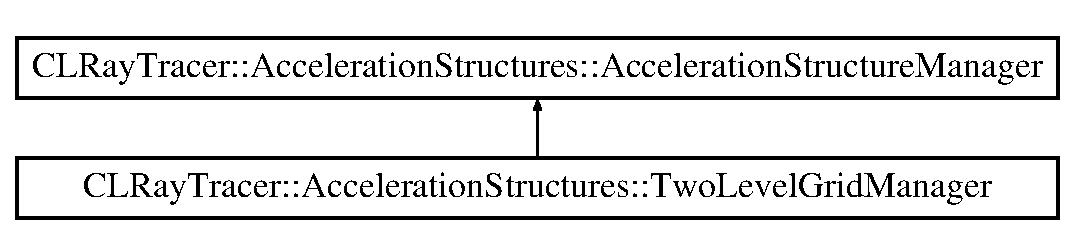
\includegraphics[height=2.000000cm]{class_c_l_ray_tracer_1_1_acceleration_structures_1_1_two_level_grid_manager}
\end{center}
\end{figure}
\subsection*{Public Member Functions}
\begin{DoxyCompactItemize}
\item 
\hyperlink{class_c_l_ray_tracer_1_1_acceleration_structures_1_1_two_level_grid_manager_ab91e464f681a2287febdb27674b82d2b}{Two\+Level\+Grid\+Manager} (const \hyperlink{class_c_l_ray_tracer_1_1_open_c_l_utils_1_1_c_l_execution_context}{Open\+C\+L\+Utils\+::\+C\+L\+Execution\+Context} \&context, const \hyperlink{class_c_l_ray_tracer_1_1_scene}{Scene} \&scene)
\item 
virtual \hyperlink{_errata_8h_a389396702f1aff6e71eb21328b0775c1}{Common\+::\+Result} \hyperlink{class_c_l_ray_tracer_1_1_acceleration_structures_1_1_two_level_grid_manager_a98f2e5e78e14ebd09f23304b730d1696}{initialize} (\hyperlink{class_c_l_ray_tracer_1_1_common_1_1_errata}{Common\+::\+Errata} \&err)
\item 
virtual \hyperlink{_errata_8h_a389396702f1aff6e71eb21328b0775c1}{Common\+::\+Result} \hyperlink{class_c_l_ray_tracer_1_1_acceleration_structures_1_1_two_level_grid_manager_a08dc7569f318a9422d69547331a31f16}{initialize\+Frame} (\hyperlink{class_c_l_ray_tracer_1_1_common_1_1_errata}{Common\+::\+Errata} \&err)
\item 
virtual \hyperlink{_errata_8h_a389396702f1aff6e71eb21328b0775c1}{Common\+::\+Result} \hyperlink{class_c_l_ray_tracer_1_1_acceleration_structures_1_1_two_level_grid_manager_a21edb29908807e8f2ba8c97d79758e05}{construct} (\hyperlink{class_c_l_ray_tracer_1_1_common_1_1_errata}{Common\+::\+Errata} \&err)
\item 
virtual \hyperlink{_errata_8h_a389396702f1aff6e71eb21328b0775c1}{Common\+::\+Result} \hyperlink{class_c_l_ray_tracer_1_1_acceleration_structures_1_1_two_level_grid_manager_a6a9f7a79568bfeb475a1ae9e1f88439d}{generate\+Contacts} (\hyperlink{struct_camera}{Camera} \&cam, \hyperlink{class_c_l_ray_tracer_1_1_common_1_1_errata}{Common\+::\+Errata} \&err)
\item 
virtual \hyperlink{_errata_8h_a389396702f1aff6e71eb21328b0775c1}{Common\+::\+Result} \hyperlink{class_c_l_ray_tracer_1_1_acceleration_structures_1_1_two_level_grid_manager_a186e22b86431d2b1c0fb92775bf6494b}{generate\+Contacts} (\hyperlink{class_c_l_ray_tracer_1_1_open_c_l_utils_1_1_c_l_buffer}{Open\+C\+L\+Utils\+::\+C\+L\+Buffer} \&rays, \hyperlink{class_c_l_ray_tracer_1_1_open_c_l_utils_1_1_c_l_buffer}{Open\+C\+L\+Utils\+::\+C\+L\+Buffer} \&contacts, const unsigned int ray\+Count, \hyperlink{class_c_l_ray_tracer_1_1_common_1_1_errata}{Common\+::\+Errata} \&err)
\item 
void \hyperlink{class_c_l_ray_tracer_1_1_acceleration_structures_1_1_two_level_grid_manager_a8781999cec61fa55d570ed5cfcafa9b0}{set\+Top\+Level\+Density} (C\+L\+\_\+\+F\+L\+O\+AT value)
\item 
void \hyperlink{class_c_l_ray_tracer_1_1_acceleration_structures_1_1_two_level_grid_manager_a22293999d15138ef66661198a926d716}{set\+Leaf\+Density} (C\+L\+\_\+\+F\+L\+O\+AT value)
\item 
C\+L\+\_\+\+F\+L\+O\+AT \hyperlink{class_c_l_ray_tracer_1_1_acceleration_structures_1_1_two_level_grid_manager_a91ff6c8c8bf49f0a1c6f474d71bd1f35}{get\+Top\+Level\+Density} () const 
\item 
C\+L\+\_\+\+F\+L\+O\+AT \hyperlink{class_c_l_ray_tracer_1_1_acceleration_structures_1_1_two_level_grid_manager_ae6a04da5ee4f28eb5402499c9055e1c7}{get\+Leaf\+Density} () const 
\item 
virtual const boost\+::shared\+\_\+ptr$<$ \hyperlink{class_c_l_ray_tracer_1_1_open_c_l_utils_1_1_c_l_buffer}{Open\+C\+L\+Utils\+::\+C\+L\+Buffer} $>$ \hyperlink{class_c_l_ray_tracer_1_1_acceleration_structures_1_1_two_level_grid_manager_ac9a677d9c2085971cd4ba758ef4be43c}{get\+Primary\+Contacts} () const 
\item 
C\+L\+\_\+\+U\+I\+N\+T3 \hyperlink{class_c_l_ray_tracer_1_1_acceleration_structures_1_1_two_level_grid_manager_a2dd1f43ec8af99c8a4fc93fcb0cab5dd}{get\+Resolution} () const 
\item 
struct \hyperlink{struct_a_a_b_b}{A\+A\+BB} \hyperlink{class_c_l_ray_tracer_1_1_acceleration_structures_1_1_two_level_grid_manager_a26228fa56e267cf336cfe26e1b278f73}{get\+Bounds} () const 
\end{DoxyCompactItemize}
\subsection*{Additional Inherited Members}


\subsection{Detailed Description}
class \hyperlink{class_c_l_ray_tracer_1_1_acceleration_structures_1_1_two_level_grid_manager}{Two\+Level\+Grid\+Manager} -\/ Provides interface for G\+PU implementation of acceleration structure\+: Two Level Grid 

\subsection{Constructor \& Destructor Documentation}
\index{C\+L\+Ray\+Tracer\+::\+Acceleration\+Structures\+::\+Two\+Level\+Grid\+Manager@{C\+L\+Ray\+Tracer\+::\+Acceleration\+Structures\+::\+Two\+Level\+Grid\+Manager}!Two\+Level\+Grid\+Manager@{Two\+Level\+Grid\+Manager}}
\index{Two\+Level\+Grid\+Manager@{Two\+Level\+Grid\+Manager}!C\+L\+Ray\+Tracer\+::\+Acceleration\+Structures\+::\+Two\+Level\+Grid\+Manager@{C\+L\+Ray\+Tracer\+::\+Acceleration\+Structures\+::\+Two\+Level\+Grid\+Manager}}
\subsubsection[{\texorpdfstring{Two\+Level\+Grid\+Manager(const Open\+C\+L\+Utils\+::\+C\+L\+Execution\+Context \&context, const Scene \&scene)}{TwoLevelGridManager(const OpenCLUtils::CLExecutionContext &context, const Scene &scene)}}]{\setlength{\rightskip}{0pt plus 5cm}C\+L\+Ray\+Tracer\+::\+Acceleration\+Structures\+::\+Two\+Level\+Grid\+Manager\+::\+Two\+Level\+Grid\+Manager (
\begin{DoxyParamCaption}
\item[{const {\bf Open\+C\+L\+Utils\+::\+C\+L\+Execution\+Context} \&}]{context, }
\item[{const {\bf Scene} \&}]{scene}
\end{DoxyParamCaption}
)}\hypertarget{class_c_l_ray_tracer_1_1_acceleration_structures_1_1_two_level_grid_manager_ab91e464f681a2287febdb27674b82d2b}{}\label{class_c_l_ray_tracer_1_1_acceleration_structures_1_1_two_level_grid_manager_ab91e464f681a2287febdb27674b82d2b}
Constructor 

\subsection{Member Function Documentation}
\index{C\+L\+Ray\+Tracer\+::\+Acceleration\+Structures\+::\+Two\+Level\+Grid\+Manager@{C\+L\+Ray\+Tracer\+::\+Acceleration\+Structures\+::\+Two\+Level\+Grid\+Manager}!construct@{construct}}
\index{construct@{construct}!C\+L\+Ray\+Tracer\+::\+Acceleration\+Structures\+::\+Two\+Level\+Grid\+Manager@{C\+L\+Ray\+Tracer\+::\+Acceleration\+Structures\+::\+Two\+Level\+Grid\+Manager}}
\subsubsection[{\texorpdfstring{construct(\+Common\+::\+Errata \&err)}{construct(Common::Errata &err)}}]{\setlength{\rightskip}{0pt plus 5cm}virtual {\bf Common\+::\+Result} C\+L\+Ray\+Tracer\+::\+Acceleration\+Structures\+::\+Two\+Level\+Grid\+Manager\+::construct (
\begin{DoxyParamCaption}
\item[{{\bf Common\+::\+Errata} \&}]{err}
\end{DoxyParamCaption}
)\hspace{0.3cm}{\ttfamily [virtual]}}\hypertarget{class_c_l_ray_tracer_1_1_acceleration_structures_1_1_two_level_grid_manager_a21edb29908807e8f2ba8c97d79758e05}{}\label{class_c_l_ray_tracer_1_1_acceleration_structures_1_1_two_level_grid_manager_a21edb29908807e8f2ba8c97d79758e05}
Constructs Two-\/\+Level Grid acceleration structure, according to associated scene state 
\begin{DoxyParams}{Parameters}
{\em err} & Error info \\
\hline
\end{DoxyParams}
\begin{DoxyReturn}{Returns}
Result of the operation\+: Success or failure 
\end{DoxyReturn}


Implements \hyperlink{class_c_l_ray_tracer_1_1_acceleration_structures_1_1_acceleration_structure_manager_a29e770ee9fa4febf24f55ecf202d352b}{C\+L\+Ray\+Tracer\+::\+Acceleration\+Structures\+::\+Acceleration\+Structure\+Manager}.

\index{C\+L\+Ray\+Tracer\+::\+Acceleration\+Structures\+::\+Two\+Level\+Grid\+Manager@{C\+L\+Ray\+Tracer\+::\+Acceleration\+Structures\+::\+Two\+Level\+Grid\+Manager}!generate\+Contacts@{generate\+Contacts}}
\index{generate\+Contacts@{generate\+Contacts}!C\+L\+Ray\+Tracer\+::\+Acceleration\+Structures\+::\+Two\+Level\+Grid\+Manager@{C\+L\+Ray\+Tracer\+::\+Acceleration\+Structures\+::\+Two\+Level\+Grid\+Manager}}
\subsubsection[{\texorpdfstring{generate\+Contacts(\+Camera \&cam, Common\+::\+Errata \&err)}{generateContacts(Camera &cam, Common::Errata &err)}}]{\setlength{\rightskip}{0pt plus 5cm}virtual {\bf Common\+::\+Result} C\+L\+Ray\+Tracer\+::\+Acceleration\+Structures\+::\+Two\+Level\+Grid\+Manager\+::generate\+Contacts (
\begin{DoxyParamCaption}
\item[{{\bf Camera} \&}]{cam, }
\item[{{\bf Common\+::\+Errata} \&}]{err}
\end{DoxyParamCaption}
)\hspace{0.3cm}{\ttfamily [virtual]}}\hypertarget{class_c_l_ray_tracer_1_1_acceleration_structures_1_1_two_level_grid_manager_a6a9f7a79568bfeb475a1ae9e1f88439d}{}\label{class_c_l_ray_tracer_1_1_acceleration_structures_1_1_two_level_grid_manager_a6a9f7a79568bfeb475a1ae9e1f88439d}
Generates hit data for viewing rays, from the constructed Two-\/\+Level Grid 
\begin{DoxyParams}{Parameters}
{\em err} & Error info \\
\hline
\end{DoxyParams}
\begin{DoxyReturn}{Returns}
Result of the operation\+: Success or failure 
\end{DoxyReturn}


Implements \hyperlink{class_c_l_ray_tracer_1_1_acceleration_structures_1_1_acceleration_structure_manager_ab94dc605d1cee5c93de253bce69f21ca}{C\+L\+Ray\+Tracer\+::\+Acceleration\+Structures\+::\+Acceleration\+Structure\+Manager}.

\index{C\+L\+Ray\+Tracer\+::\+Acceleration\+Structures\+::\+Two\+Level\+Grid\+Manager@{C\+L\+Ray\+Tracer\+::\+Acceleration\+Structures\+::\+Two\+Level\+Grid\+Manager}!generate\+Contacts@{generate\+Contacts}}
\index{generate\+Contacts@{generate\+Contacts}!C\+L\+Ray\+Tracer\+::\+Acceleration\+Structures\+::\+Two\+Level\+Grid\+Manager@{C\+L\+Ray\+Tracer\+::\+Acceleration\+Structures\+::\+Two\+Level\+Grid\+Manager}}
\subsubsection[{\texorpdfstring{generate\+Contacts(\+Open\+C\+L\+Utils\+::\+C\+L\+Buffer \&rays, Open\+C\+L\+Utils\+::\+C\+L\+Buffer \&contacts, const unsigned int ray\+Count, Common\+::\+Errata \&err)}{generateContacts(OpenCLUtils::CLBuffer &rays, OpenCLUtils::CLBuffer &contacts, const unsigned int rayCount, Common::Errata &err)}}]{\setlength{\rightskip}{0pt plus 5cm}virtual {\bf Common\+::\+Result} C\+L\+Ray\+Tracer\+::\+Acceleration\+Structures\+::\+Two\+Level\+Grid\+Manager\+::generate\+Contacts (
\begin{DoxyParamCaption}
\item[{{\bf Open\+C\+L\+Utils\+::\+C\+L\+Buffer} \&}]{rays, }
\item[{{\bf Open\+C\+L\+Utils\+::\+C\+L\+Buffer} \&}]{contacts, }
\item[{const unsigned int}]{ray\+Count, }
\item[{{\bf Common\+::\+Errata} \&}]{err}
\end{DoxyParamCaption}
)\hspace{0.3cm}{\ttfamily [virtual]}}\hypertarget{class_c_l_ray_tracer_1_1_acceleration_structures_1_1_two_level_grid_manager_a186e22b86431d2b1c0fb92775bf6494b}{}\label{class_c_l_ray_tracer_1_1_acceleration_structures_1_1_two_level_grid_manager_a186e22b86431d2b1c0fb92775bf6494b}
Generates contacts for rays and fills the contacts array 
\begin{DoxyParams}{Parameters}
{\em rays} & The rays to be traced -\/ A device memory buffer object that contains rays as struct \hyperlink{struct_ray}{Ray} \\
\hline
{\em contact} & The target device memory that will contain the result -\/ For each ray rays\mbox{[}i\mbox{]} the buffer will contain data about its closest intersection with object in the scene as contacts\mbox{[}i\mbox{]}. The contact data will be stored as struct \hyperlink{struct_contact}{Contact} \\
\hline
{\em ray\+Count} & The number of rays to trace \\
\hline
{\em err} & Error info \\
\hline
\end{DoxyParams}
\begin{DoxyReturn}{Returns}
Result of the operation\+: Success or failure 
\end{DoxyReturn}


Implements \hyperlink{class_c_l_ray_tracer_1_1_acceleration_structures_1_1_acceleration_structure_manager_aaa7b1d615a20126278ef27f0a5f3215c}{C\+L\+Ray\+Tracer\+::\+Acceleration\+Structures\+::\+Acceleration\+Structure\+Manager}.

\index{C\+L\+Ray\+Tracer\+::\+Acceleration\+Structures\+::\+Two\+Level\+Grid\+Manager@{C\+L\+Ray\+Tracer\+::\+Acceleration\+Structures\+::\+Two\+Level\+Grid\+Manager}!get\+Bounds@{get\+Bounds}}
\index{get\+Bounds@{get\+Bounds}!C\+L\+Ray\+Tracer\+::\+Acceleration\+Structures\+::\+Two\+Level\+Grid\+Manager@{C\+L\+Ray\+Tracer\+::\+Acceleration\+Structures\+::\+Two\+Level\+Grid\+Manager}}
\subsubsection[{\texorpdfstring{get\+Bounds() const }{getBounds() const }}]{\setlength{\rightskip}{0pt plus 5cm}struct {\bf A\+A\+BB} C\+L\+Ray\+Tracer\+::\+Acceleration\+Structures\+::\+Two\+Level\+Grid\+Manager\+::get\+Bounds (
\begin{DoxyParamCaption}
{}
\end{DoxyParamCaption}
) const}\hypertarget{class_c_l_ray_tracer_1_1_acceleration_structures_1_1_two_level_grid_manager_a26228fa56e267cf336cfe26e1b278f73}{}\label{class_c_l_ray_tracer_1_1_acceleration_structures_1_1_two_level_grid_manager_a26228fa56e267cf336cfe26e1b278f73}
Calculates internal grid data for use on G\+PU \begin{DoxyReturn}{Returns}

\end{DoxyReturn}
\index{C\+L\+Ray\+Tracer\+::\+Acceleration\+Structures\+::\+Two\+Level\+Grid\+Manager@{C\+L\+Ray\+Tracer\+::\+Acceleration\+Structures\+::\+Two\+Level\+Grid\+Manager}!get\+Leaf\+Density@{get\+Leaf\+Density}}
\index{get\+Leaf\+Density@{get\+Leaf\+Density}!C\+L\+Ray\+Tracer\+::\+Acceleration\+Structures\+::\+Two\+Level\+Grid\+Manager@{C\+L\+Ray\+Tracer\+::\+Acceleration\+Structures\+::\+Two\+Level\+Grid\+Manager}}
\subsubsection[{\texorpdfstring{get\+Leaf\+Density() const }{getLeafDensity() const }}]{\setlength{\rightskip}{0pt plus 5cm}C\+L\+\_\+\+F\+L\+O\+AT C\+L\+Ray\+Tracer\+::\+Acceleration\+Structures\+::\+Two\+Level\+Grid\+Manager\+::get\+Leaf\+Density (
\begin{DoxyParamCaption}
{}
\end{DoxyParamCaption}
) const\hspace{0.3cm}{\ttfamily [inline]}}\hypertarget{class_c_l_ray_tracer_1_1_acceleration_structures_1_1_two_level_grid_manager_ae6a04da5ee4f28eb5402499c9055e1c7}{}\label{class_c_l_ray_tracer_1_1_acceleration_structures_1_1_two_level_grid_manager_ae6a04da5ee4f28eb5402499c9055e1c7}
Gets the leaf level density parameter of the grid, for leaf level resolution calculation \index{C\+L\+Ray\+Tracer\+::\+Acceleration\+Structures\+::\+Two\+Level\+Grid\+Manager@{C\+L\+Ray\+Tracer\+::\+Acceleration\+Structures\+::\+Two\+Level\+Grid\+Manager}!get\+Primary\+Contacts@{get\+Primary\+Contacts}}
\index{get\+Primary\+Contacts@{get\+Primary\+Contacts}!C\+L\+Ray\+Tracer\+::\+Acceleration\+Structures\+::\+Two\+Level\+Grid\+Manager@{C\+L\+Ray\+Tracer\+::\+Acceleration\+Structures\+::\+Two\+Level\+Grid\+Manager}}
\subsubsection[{\texorpdfstring{get\+Primary\+Contacts() const }{getPrimaryContacts() const }}]{\setlength{\rightskip}{0pt plus 5cm}virtual const boost\+::shared\+\_\+ptr$<${\bf Open\+C\+L\+Utils\+::\+C\+L\+Buffer}$>$ C\+L\+Ray\+Tracer\+::\+Acceleration\+Structures\+::\+Two\+Level\+Grid\+Manager\+::get\+Primary\+Contacts (
\begin{DoxyParamCaption}
{}
\end{DoxyParamCaption}
) const\hspace{0.3cm}{\ttfamily [inline]}, {\ttfamily [virtual]}}\hypertarget{class_c_l_ray_tracer_1_1_acceleration_structures_1_1_two_level_grid_manager_ac9a677d9c2085971cd4ba758ef4be43c}{}\label{class_c_l_ray_tracer_1_1_acceleration_structures_1_1_two_level_grid_manager_ac9a677d9c2085971cd4ba758ef4be43c}
Gets the device memory buffer for primary rays -\/ result of generate\+Contacts function 

Implements \hyperlink{class_c_l_ray_tracer_1_1_acceleration_structures_1_1_acceleration_structure_manager_aeaaccc5dde154278325f1596b7bcde31}{C\+L\+Ray\+Tracer\+::\+Acceleration\+Structures\+::\+Acceleration\+Structure\+Manager}.

\index{C\+L\+Ray\+Tracer\+::\+Acceleration\+Structures\+::\+Two\+Level\+Grid\+Manager@{C\+L\+Ray\+Tracer\+::\+Acceleration\+Structures\+::\+Two\+Level\+Grid\+Manager}!get\+Resolution@{get\+Resolution}}
\index{get\+Resolution@{get\+Resolution}!C\+L\+Ray\+Tracer\+::\+Acceleration\+Structures\+::\+Two\+Level\+Grid\+Manager@{C\+L\+Ray\+Tracer\+::\+Acceleration\+Structures\+::\+Two\+Level\+Grid\+Manager}}
\subsubsection[{\texorpdfstring{get\+Resolution() const }{getResolution() const }}]{\setlength{\rightskip}{0pt plus 5cm}C\+L\+\_\+\+U\+I\+N\+T3 C\+L\+Ray\+Tracer\+::\+Acceleration\+Structures\+::\+Two\+Level\+Grid\+Manager\+::get\+Resolution (
\begin{DoxyParamCaption}
{}
\end{DoxyParamCaption}
) const}\hypertarget{class_c_l_ray_tracer_1_1_acceleration_structures_1_1_two_level_grid_manager_a2dd1f43ec8af99c8a4fc93fcb0cab5dd}{}\label{class_c_l_ray_tracer_1_1_acceleration_structures_1_1_two_level_grid_manager_a2dd1f43ec8af99c8a4fc93fcb0cab5dd}
Calculates grid resolution according to grid properties \begin{DoxyReturn}{Returns}
Grid resolution 
\end{DoxyReturn}
\index{C\+L\+Ray\+Tracer\+::\+Acceleration\+Structures\+::\+Two\+Level\+Grid\+Manager@{C\+L\+Ray\+Tracer\+::\+Acceleration\+Structures\+::\+Two\+Level\+Grid\+Manager}!get\+Top\+Level\+Density@{get\+Top\+Level\+Density}}
\index{get\+Top\+Level\+Density@{get\+Top\+Level\+Density}!C\+L\+Ray\+Tracer\+::\+Acceleration\+Structures\+::\+Two\+Level\+Grid\+Manager@{C\+L\+Ray\+Tracer\+::\+Acceleration\+Structures\+::\+Two\+Level\+Grid\+Manager}}
\subsubsection[{\texorpdfstring{get\+Top\+Level\+Density() const }{getTopLevelDensity() const }}]{\setlength{\rightskip}{0pt plus 5cm}C\+L\+\_\+\+F\+L\+O\+AT C\+L\+Ray\+Tracer\+::\+Acceleration\+Structures\+::\+Two\+Level\+Grid\+Manager\+::get\+Top\+Level\+Density (
\begin{DoxyParamCaption}
{}
\end{DoxyParamCaption}
) const\hspace{0.3cm}{\ttfamily [inline]}}\hypertarget{class_c_l_ray_tracer_1_1_acceleration_structures_1_1_two_level_grid_manager_a91ff6c8c8bf49f0a1c6f474d71bd1f35}{}\label{class_c_l_ray_tracer_1_1_acceleration_structures_1_1_two_level_grid_manager_a91ff6c8c8bf49f0a1c6f474d71bd1f35}
Gets the top level density parameter of the grid, for top level resolution calculation \index{C\+L\+Ray\+Tracer\+::\+Acceleration\+Structures\+::\+Two\+Level\+Grid\+Manager@{C\+L\+Ray\+Tracer\+::\+Acceleration\+Structures\+::\+Two\+Level\+Grid\+Manager}!initialize@{initialize}}
\index{initialize@{initialize}!C\+L\+Ray\+Tracer\+::\+Acceleration\+Structures\+::\+Two\+Level\+Grid\+Manager@{C\+L\+Ray\+Tracer\+::\+Acceleration\+Structures\+::\+Two\+Level\+Grid\+Manager}}
\subsubsection[{\texorpdfstring{initialize(\+Common\+::\+Errata \&err)}{initialize(Common::Errata &err)}}]{\setlength{\rightskip}{0pt plus 5cm}virtual {\bf Common\+::\+Result} C\+L\+Ray\+Tracer\+::\+Acceleration\+Structures\+::\+Two\+Level\+Grid\+Manager\+::initialize (
\begin{DoxyParamCaption}
\item[{{\bf Common\+::\+Errata} \&}]{err}
\end{DoxyParamCaption}
)\hspace{0.3cm}{\ttfamily [virtual]}}\hypertarget{class_c_l_ray_tracer_1_1_acceleration_structures_1_1_two_level_grid_manager_a98f2e5e78e14ebd09f23304b730d1696}{}\label{class_c_l_ray_tracer_1_1_acceleration_structures_1_1_two_level_grid_manager_a98f2e5e78e14ebd09f23304b730d1696}
Performs main initialization of the Two Level Grid structure. This initialization shoud be performed just once per instance. 
\begin{DoxyParams}{Parameters}
{\em err} & Error info \\
\hline
\end{DoxyParams}
\begin{DoxyReturn}{Returns}
Result of the operation\+: Success or failure 
\end{DoxyReturn}


Implements \hyperlink{class_c_l_ray_tracer_1_1_acceleration_structures_1_1_acceleration_structure_manager_a14a5bacd261ea5c3e541ae531a128e4d}{C\+L\+Ray\+Tracer\+::\+Acceleration\+Structures\+::\+Acceleration\+Structure\+Manager}.

\index{C\+L\+Ray\+Tracer\+::\+Acceleration\+Structures\+::\+Two\+Level\+Grid\+Manager@{C\+L\+Ray\+Tracer\+::\+Acceleration\+Structures\+::\+Two\+Level\+Grid\+Manager}!initialize\+Frame@{initialize\+Frame}}
\index{initialize\+Frame@{initialize\+Frame}!C\+L\+Ray\+Tracer\+::\+Acceleration\+Structures\+::\+Two\+Level\+Grid\+Manager@{C\+L\+Ray\+Tracer\+::\+Acceleration\+Structures\+::\+Two\+Level\+Grid\+Manager}}
\subsubsection[{\texorpdfstring{initialize\+Frame(\+Common\+::\+Errata \&err)}{initializeFrame(Common::Errata &err)}}]{\setlength{\rightskip}{0pt plus 5cm}virtual {\bf Common\+::\+Result} C\+L\+Ray\+Tracer\+::\+Acceleration\+Structures\+::\+Two\+Level\+Grid\+Manager\+::initialize\+Frame (
\begin{DoxyParamCaption}
\item[{{\bf Common\+::\+Errata} \&}]{err}
\end{DoxyParamCaption}
)\hspace{0.3cm}{\ttfamily [virtual]}}\hypertarget{class_c_l_ray_tracer_1_1_acceleration_structures_1_1_two_level_grid_manager_a08dc7569f318a9422d69547331a31f16}{}\label{class_c_l_ray_tracer_1_1_acceleration_structures_1_1_two_level_grid_manager_a08dc7569f318a9422d69547331a31f16}
Performs initialization of a frame for Two Level Grid acceleration structure This initialization shoud be performed before each frame. Grid property change will take effect only after execution of this function. 
\begin{DoxyParams}{Parameters}
{\em err} & Error info \\
\hline
\end{DoxyParams}
\begin{DoxyReturn}{Returns}
Result of the operation\+: Success or failure 
\end{DoxyReturn}


Implements \hyperlink{class_c_l_ray_tracer_1_1_acceleration_structures_1_1_acceleration_structure_manager_a3707d7588ce68855e6f086022025f1ea}{C\+L\+Ray\+Tracer\+::\+Acceleration\+Structures\+::\+Acceleration\+Structure\+Manager}.

\index{C\+L\+Ray\+Tracer\+::\+Acceleration\+Structures\+::\+Two\+Level\+Grid\+Manager@{C\+L\+Ray\+Tracer\+::\+Acceleration\+Structures\+::\+Two\+Level\+Grid\+Manager}!set\+Leaf\+Density@{set\+Leaf\+Density}}
\index{set\+Leaf\+Density@{set\+Leaf\+Density}!C\+L\+Ray\+Tracer\+::\+Acceleration\+Structures\+::\+Two\+Level\+Grid\+Manager@{C\+L\+Ray\+Tracer\+::\+Acceleration\+Structures\+::\+Two\+Level\+Grid\+Manager}}
\subsubsection[{\texorpdfstring{set\+Leaf\+Density(\+C\+L\+\_\+\+F\+L\+O\+A\+T value)}{setLeafDensity(CL_FLOAT value)}}]{\setlength{\rightskip}{0pt plus 5cm}void C\+L\+Ray\+Tracer\+::\+Acceleration\+Structures\+::\+Two\+Level\+Grid\+Manager\+::set\+Leaf\+Density (
\begin{DoxyParamCaption}
\item[{C\+L\+\_\+\+F\+L\+O\+AT}]{value}
\end{DoxyParamCaption}
)\hspace{0.3cm}{\ttfamily [inline]}}\hypertarget{class_c_l_ray_tracer_1_1_acceleration_structures_1_1_two_level_grid_manager_a22293999d15138ef66661198a926d716}{}\label{class_c_l_ray_tracer_1_1_acceleration_structures_1_1_two_level_grid_manager_a22293999d15138ef66661198a926d716}
Sets the leaf level density parameter of the grid, for leaf level resolution calculation \index{C\+L\+Ray\+Tracer\+::\+Acceleration\+Structures\+::\+Two\+Level\+Grid\+Manager@{C\+L\+Ray\+Tracer\+::\+Acceleration\+Structures\+::\+Two\+Level\+Grid\+Manager}!set\+Top\+Level\+Density@{set\+Top\+Level\+Density}}
\index{set\+Top\+Level\+Density@{set\+Top\+Level\+Density}!C\+L\+Ray\+Tracer\+::\+Acceleration\+Structures\+::\+Two\+Level\+Grid\+Manager@{C\+L\+Ray\+Tracer\+::\+Acceleration\+Structures\+::\+Two\+Level\+Grid\+Manager}}
\subsubsection[{\texorpdfstring{set\+Top\+Level\+Density(\+C\+L\+\_\+\+F\+L\+O\+A\+T value)}{setTopLevelDensity(CL_FLOAT value)}}]{\setlength{\rightskip}{0pt plus 5cm}void C\+L\+Ray\+Tracer\+::\+Acceleration\+Structures\+::\+Two\+Level\+Grid\+Manager\+::set\+Top\+Level\+Density (
\begin{DoxyParamCaption}
\item[{C\+L\+\_\+\+F\+L\+O\+AT}]{value}
\end{DoxyParamCaption}
)\hspace{0.3cm}{\ttfamily [inline]}}\hypertarget{class_c_l_ray_tracer_1_1_acceleration_structures_1_1_two_level_grid_manager_a8781999cec61fa55d570ed5cfcafa9b0}{}\label{class_c_l_ray_tracer_1_1_acceleration_structures_1_1_two_level_grid_manager_a8781999cec61fa55d570ed5cfcafa9b0}
Sets the top level density parameter of the grid, for top level resolution calculation 

The documentation for this class was generated from the following file\+:\begin{DoxyCompactItemize}
\item 
Include/\+Algorithms/\hyperlink{_two_level_grid_manager_8h}{Two\+Level\+Grid\+Manager.\+h}\end{DoxyCompactItemize}

\hypertarget{class_c_l_ray_tracer_1_1_open_c_l_utils_1_1_c_l_device_1_1_work_group_dimensions}{}\section{C\+L\+Ray\+Tracer\+:\+:Open\+C\+L\+Utils\+:\+:C\+L\+Device\+:\+:Work\+Group\+Dimensions Class Reference}
\label{class_c_l_ray_tracer_1_1_open_c_l_utils_1_1_c_l_device_1_1_work_group_dimensions}\index{C\+L\+Ray\+Tracer\+::\+Open\+C\+L\+Utils\+::\+C\+L\+Device\+::\+Work\+Group\+Dimensions@{C\+L\+Ray\+Tracer\+::\+Open\+C\+L\+Utils\+::\+C\+L\+Device\+::\+Work\+Group\+Dimensions}}


{\ttfamily \#include $<$C\+L\+Interface.\+h$>$}

\subsection*{Public Member Functions}
\begin{DoxyCompactItemize}
\item 
\hyperlink{class_c_l_ray_tracer_1_1_open_c_l_utils_1_1_c_l_device_1_1_work_group_dimensions_ae5cf1324551c302c61241ee3f4546fd8}{Work\+Group\+Dimensions} (cl\+\_\+device\+\_\+id device\+Id)
\item 
\hyperlink{class_c_l_ray_tracer_1_1_open_c_l_utils_1_1_c_l_device_1_1_work_group_dimensions_ac609b4c595f2eafaa7426b0af8fa75a7}{D\+E\+V\+I\+C\+E\+\_\+\+P\+R\+O\+P\+E\+R\+T\+Y\+\_\+\+G\+E\+T\+T\+ER} (get\+Max\+Work\+Group\+Size, C\+L\+\_\+\+D\+E\+V\+I\+C\+E\+\_\+\+M\+A\+X\+\_\+\+W\+O\+R\+K\+\_\+\+G\+R\+O\+U\+P\+\_\+\+S\+I\+ZE, size\+\_\+t)
\item 
\hyperlink{class_c_l_ray_tracer_1_1_open_c_l_utils_1_1_c_l_device_1_1_work_group_dimensions_a22779ba8b6eb8f80a61a1500c89b3fc2}{D\+E\+V\+I\+C\+E\+\_\+\+P\+R\+O\+P\+E\+R\+T\+Y\+\_\+\+G\+E\+T\+T\+ER} (get\+Max\+Work\+Item\+Dimensions, C\+L\+\_\+\+D\+E\+V\+I\+C\+E\+\_\+\+M\+A\+X\+\_\+\+W\+O\+R\+K\+\_\+\+I\+T\+E\+M\+\_\+\+D\+I\+M\+E\+N\+S\+I\+O\+NS, cl\+\_\+uint)
\item 
\hyperlink{_errata_8h_a389396702f1aff6e71eb21328b0775c1}{Common\+::\+Result} \hyperlink{class_c_l_ray_tracer_1_1_open_c_l_utils_1_1_c_l_device_1_1_work_group_dimensions_ae54257325fdf3e13bac148d01ba5e0bb}{get\+Max\+Work\+Item\+Sizes} (boost\+::shared\+\_\+array$<$ size\+\_\+t $>$ \&value, \hyperlink{class_c_l_ray_tracer_1_1_common_1_1_errata}{Common\+::\+Errata} \&err) const 
\end{DoxyCompactItemize}


\subsection{Detailed Description}
Class \hyperlink{class_c_l_ray_tracer_1_1_open_c_l_utils_1_1_c_l_device_1_1_work_group_dimensions}{Work\+Group\+Dimensions} groups device properties related to work group dimensions constrainsts on this device 

\subsection{Constructor \& Destructor Documentation}
\index{C\+L\+Ray\+Tracer\+::\+Open\+C\+L\+Utils\+::\+C\+L\+Device\+::\+Work\+Group\+Dimensions@{C\+L\+Ray\+Tracer\+::\+Open\+C\+L\+Utils\+::\+C\+L\+Device\+::\+Work\+Group\+Dimensions}!Work\+Group\+Dimensions@{Work\+Group\+Dimensions}}
\index{Work\+Group\+Dimensions@{Work\+Group\+Dimensions}!C\+L\+Ray\+Tracer\+::\+Open\+C\+L\+Utils\+::\+C\+L\+Device\+::\+Work\+Group\+Dimensions@{C\+L\+Ray\+Tracer\+::\+Open\+C\+L\+Utils\+::\+C\+L\+Device\+::\+Work\+Group\+Dimensions}}
\subsubsection[{\texorpdfstring{Work\+Group\+Dimensions(cl\+\_\+device\+\_\+id device\+Id)}{WorkGroupDimensions(cl_device_id deviceId)}}]{\setlength{\rightskip}{0pt plus 5cm}C\+L\+Ray\+Tracer\+::\+Open\+C\+L\+Utils\+::\+C\+L\+Device\+::\+Work\+Group\+Dimensions\+::\+Work\+Group\+Dimensions (
\begin{DoxyParamCaption}
\item[{cl\+\_\+device\+\_\+id}]{device\+Id}
\end{DoxyParamCaption}
)\hspace{0.3cm}{\ttfamily [inline]}}\hypertarget{class_c_l_ray_tracer_1_1_open_c_l_utils_1_1_c_l_device_1_1_work_group_dimensions_ae5cf1324551c302c61241ee3f4546fd8}{}\label{class_c_l_ray_tracer_1_1_open_c_l_utils_1_1_c_l_device_1_1_work_group_dimensions_ae5cf1324551c302c61241ee3f4546fd8}
Constructor 

\subsection{Member Function Documentation}
\index{C\+L\+Ray\+Tracer\+::\+Open\+C\+L\+Utils\+::\+C\+L\+Device\+::\+Work\+Group\+Dimensions@{C\+L\+Ray\+Tracer\+::\+Open\+C\+L\+Utils\+::\+C\+L\+Device\+::\+Work\+Group\+Dimensions}!D\+E\+V\+I\+C\+E\+\_\+\+P\+R\+O\+P\+E\+R\+T\+Y\+\_\+\+G\+E\+T\+T\+ER@{D\+E\+V\+I\+C\+E\+\_\+\+P\+R\+O\+P\+E\+R\+T\+Y\+\_\+\+G\+E\+T\+T\+ER}}
\index{D\+E\+V\+I\+C\+E\+\_\+\+P\+R\+O\+P\+E\+R\+T\+Y\+\_\+\+G\+E\+T\+T\+ER@{D\+E\+V\+I\+C\+E\+\_\+\+P\+R\+O\+P\+E\+R\+T\+Y\+\_\+\+G\+E\+T\+T\+ER}!C\+L\+Ray\+Tracer\+::\+Open\+C\+L\+Utils\+::\+C\+L\+Device\+::\+Work\+Group\+Dimensions@{C\+L\+Ray\+Tracer\+::\+Open\+C\+L\+Utils\+::\+C\+L\+Device\+::\+Work\+Group\+Dimensions}}
\subsubsection[{\texorpdfstring{D\+E\+V\+I\+C\+E\+\_\+\+P\+R\+O\+P\+E\+R\+T\+Y\+\_\+\+G\+E\+T\+T\+E\+R(get\+Max\+Work\+Group\+Size, C\+L\+\_\+\+D\+E\+V\+I\+C\+E\+\_\+\+M\+A\+X\+\_\+\+W\+O\+R\+K\+\_\+\+G\+R\+O\+U\+P\+\_\+\+S\+I\+Z\+E, size\+\_\+t)}{DEVICE_PROPERTY_GETTER(getMaxWorkGroupSize, CL_DEVICE_MAX_WORK_GROUP_SIZE, size_t)}}]{\setlength{\rightskip}{0pt plus 5cm}C\+L\+Ray\+Tracer\+::\+Open\+C\+L\+Utils\+::\+C\+L\+Device\+::\+Work\+Group\+Dimensions\+::\+D\+E\+V\+I\+C\+E\+\_\+\+P\+R\+O\+P\+E\+R\+T\+Y\+\_\+\+G\+E\+T\+T\+ER (
\begin{DoxyParamCaption}
\item[{get\+Max\+Work\+Group\+Size}]{, }
\item[{C\+L\+\_\+\+D\+E\+V\+I\+C\+E\+\_\+\+M\+A\+X\+\_\+\+W\+O\+R\+K\+\_\+\+G\+R\+O\+U\+P\+\_\+\+S\+I\+ZE}]{, }
\item[{size\+\_\+t}]{}
\end{DoxyParamCaption}
)}\hypertarget{class_c_l_ray_tracer_1_1_open_c_l_utils_1_1_c_l_device_1_1_work_group_dimensions_ac609b4c595f2eafaa7426b0af8fa75a7}{}\label{class_c_l_ray_tracer_1_1_open_c_l_utils_1_1_c_l_device_1_1_work_group_dimensions_ac609b4c595f2eafaa7426b0af8fa75a7}
Retrieves property of Open\+CL Device\+: Maximum number of work-\/items in a work-\/group executing a kernel using the data parallel execution model. 
\begin{DoxyParams}[1]{Parameters}
\mbox{\tt out}  & {\em } & \\
\hline
\end{DoxyParams}
\index{C\+L\+Ray\+Tracer\+::\+Open\+C\+L\+Utils\+::\+C\+L\+Device\+::\+Work\+Group\+Dimensions@{C\+L\+Ray\+Tracer\+::\+Open\+C\+L\+Utils\+::\+C\+L\+Device\+::\+Work\+Group\+Dimensions}!D\+E\+V\+I\+C\+E\+\_\+\+P\+R\+O\+P\+E\+R\+T\+Y\+\_\+\+G\+E\+T\+T\+ER@{D\+E\+V\+I\+C\+E\+\_\+\+P\+R\+O\+P\+E\+R\+T\+Y\+\_\+\+G\+E\+T\+T\+ER}}
\index{D\+E\+V\+I\+C\+E\+\_\+\+P\+R\+O\+P\+E\+R\+T\+Y\+\_\+\+G\+E\+T\+T\+ER@{D\+E\+V\+I\+C\+E\+\_\+\+P\+R\+O\+P\+E\+R\+T\+Y\+\_\+\+G\+E\+T\+T\+ER}!C\+L\+Ray\+Tracer\+::\+Open\+C\+L\+Utils\+::\+C\+L\+Device\+::\+Work\+Group\+Dimensions@{C\+L\+Ray\+Tracer\+::\+Open\+C\+L\+Utils\+::\+C\+L\+Device\+::\+Work\+Group\+Dimensions}}
\subsubsection[{\texorpdfstring{D\+E\+V\+I\+C\+E\+\_\+\+P\+R\+O\+P\+E\+R\+T\+Y\+\_\+\+G\+E\+T\+T\+E\+R(get\+Max\+Work\+Item\+Dimensions, C\+L\+\_\+\+D\+E\+V\+I\+C\+E\+\_\+\+M\+A\+X\+\_\+\+W\+O\+R\+K\+\_\+\+I\+T\+E\+M\+\_\+\+D\+I\+M\+E\+N\+S\+I\+O\+N\+S, cl\+\_\+uint)}{DEVICE_PROPERTY_GETTER(getMaxWorkItemDimensions, CL_DEVICE_MAX_WORK_ITEM_DIMENSIONS, cl_uint)}}]{\setlength{\rightskip}{0pt plus 5cm}C\+L\+Ray\+Tracer\+::\+Open\+C\+L\+Utils\+::\+C\+L\+Device\+::\+Work\+Group\+Dimensions\+::\+D\+E\+V\+I\+C\+E\+\_\+\+P\+R\+O\+P\+E\+R\+T\+Y\+\_\+\+G\+E\+T\+T\+ER (
\begin{DoxyParamCaption}
\item[{get\+Max\+Work\+Item\+Dimensions}]{, }
\item[{C\+L\+\_\+\+D\+E\+V\+I\+C\+E\+\_\+\+M\+A\+X\+\_\+\+W\+O\+R\+K\+\_\+\+I\+T\+E\+M\+\_\+\+D\+I\+M\+E\+N\+S\+I\+O\+NS}]{, }
\item[{cl\+\_\+uint}]{}
\end{DoxyParamCaption}
)}\hypertarget{class_c_l_ray_tracer_1_1_open_c_l_utils_1_1_c_l_device_1_1_work_group_dimensions_a22779ba8b6eb8f80a61a1500c89b3fc2}{}\label{class_c_l_ray_tracer_1_1_open_c_l_utils_1_1_c_l_device_1_1_work_group_dimensions_a22779ba8b6eb8f80a61a1500c89b3fc2}
Retrieves property of Open\+CL Device\+: Maximum dimensions that specify the global and local work-\/item I\+Ds used by the data parallel execution model. 
\begin{DoxyParams}[1]{Parameters}
\mbox{\tt out}  & {\em } & \\
\hline
\end{DoxyParams}
\index{C\+L\+Ray\+Tracer\+::\+Open\+C\+L\+Utils\+::\+C\+L\+Device\+::\+Work\+Group\+Dimensions@{C\+L\+Ray\+Tracer\+::\+Open\+C\+L\+Utils\+::\+C\+L\+Device\+::\+Work\+Group\+Dimensions}!get\+Max\+Work\+Item\+Sizes@{get\+Max\+Work\+Item\+Sizes}}
\index{get\+Max\+Work\+Item\+Sizes@{get\+Max\+Work\+Item\+Sizes}!C\+L\+Ray\+Tracer\+::\+Open\+C\+L\+Utils\+::\+C\+L\+Device\+::\+Work\+Group\+Dimensions@{C\+L\+Ray\+Tracer\+::\+Open\+C\+L\+Utils\+::\+C\+L\+Device\+::\+Work\+Group\+Dimensions}}
\subsubsection[{\texorpdfstring{get\+Max\+Work\+Item\+Sizes(boost\+::shared\+\_\+array$<$ size\+\_\+t $>$ \&value, Common\+::\+Errata \&err) const }{getMaxWorkItemSizes(boost::shared_array< size_t > &value, Common::Errata &err) const }}]{\setlength{\rightskip}{0pt plus 5cm}{\bf Common\+::\+Result} C\+L\+Ray\+Tracer\+::\+Open\+C\+L\+Utils\+::\+C\+L\+Device\+::\+Work\+Group\+Dimensions\+::get\+Max\+Work\+Item\+Sizes (
\begin{DoxyParamCaption}
\item[{boost\+::shared\+\_\+array$<$ size\+\_\+t $>$ \&}]{value, }
\item[{{\bf Common\+::\+Errata} \&}]{err}
\end{DoxyParamCaption}
) const\hspace{0.3cm}{\ttfamily [inline]}}\hypertarget{class_c_l_ray_tracer_1_1_open_c_l_utils_1_1_c_l_device_1_1_work_group_dimensions_ae54257325fdf3e13bac148d01ba5e0bb}{}\label{class_c_l_ray_tracer_1_1_open_c_l_utils_1_1_c_l_device_1_1_work_group_dimensions_ae54257325fdf3e13bac148d01ba5e0bb}
Retrieves property of Open\+CL Device\+: Maximum number of work-\/items that can be specified in each dimension of the work-\/group 
\begin{DoxyParams}[1]{Parameters}
\mbox{\tt out}  & {\em } & \\
\hline
\end{DoxyParams}


The documentation for this class was generated from the following file\+:\begin{DoxyCompactItemize}
\item 
Include/\+Open\+C\+L\+Utils/C\+L\+Interface.\+h\end{DoxyCompactItemize}

\chapter{File Documentation}
\hypertarget{_acceleration_structure_manager_8h}{}\section{Include/\+Algorithms/\+Acceleration\+Structure\+Manager.h File Reference}
\label{_acceleration_structure_manager_8h}\index{Include/\+Algorithms/\+Acceleration\+Structure\+Manager.\+h@{Include/\+Algorithms/\+Acceleration\+Structure\+Manager.\+h}}
{\ttfamily \#include $<$common\textbackslash{}\+Errata.\+h$>$}\\*
\subsection*{Classes}
\begin{DoxyCompactItemize}
\item 
class \hyperlink{class_c_l_ray_tracer_1_1_acceleration_structures_1_1_acceleration_structure_manager}{C\+L\+Ray\+Tracer\+::\+Acceleration\+Structures\+::\+Acceleration\+Structure\+Manager}
\end{DoxyCompactItemize}


\subsection{Detailed Description}
\begin{DoxyAuthor}{Author}
Timur Sizov \href{mailto:timorgizer@gmail.com}{\tt timorgizer@gmail.\+com} 
\end{DoxyAuthor}
\begin{DoxyVersion}{Version}
0.\+6
\end{DoxyVersion}
\hypertarget{_scene_8h_LICENSE}{}\subsection{L\+I\+C\+E\+N\+SE}\label{_scene_8h_LICENSE}
Copyright (c) 2016 Timur Sizov

Permission is hereby granted, free of charge, to any person obtaining a copy of this software and associated documentation files (the \char`\"{}\+Software\char`\"{}), to deal in the Software without restriction, including without limitation the rights to use, copy, modify, merge, publish, distribute, sublicense, and/or sell copies of the Software, and to permit persons to whom the Software is furnished to do so, subject to the following conditions\+: The above copyright notice and this permission notice shall be included in all copies or substantial portions of the Software.

T\+HE S\+O\+F\+T\+W\+A\+RE IS P\+R\+O\+V\+I\+D\+ED \char`\"{}\+A\+S I\+S\char`\"{}, W\+I\+T\+H\+O\+UT W\+A\+R\+R\+A\+N\+TY OF A\+NY K\+I\+ND, E\+X\+P\+R\+E\+SS OR I\+M\+P\+L\+I\+ED, I\+N\+C\+L\+U\+D\+I\+NG B\+UT N\+OT L\+I\+M\+I\+T\+ED TO T\+HE W\+A\+R\+R\+A\+N\+T\+I\+ES OF M\+E\+R\+C\+H\+A\+N\+T\+A\+B\+I\+L\+I\+TY, F\+I\+T\+N\+E\+SS F\+OR A P\+A\+R\+T\+I\+C\+U\+L\+AR P\+U\+R\+P\+O\+SE A\+ND N\+O\+N\+I\+N\+F\+R\+I\+N\+G\+E\+M\+E\+NT. IN NO E\+V\+E\+NT S\+H\+A\+LL T\+HE A\+U\+T\+H\+O\+RS OR C\+O\+P\+Y\+R\+I\+G\+HT H\+O\+L\+D\+E\+RS BE L\+I\+A\+B\+LE F\+OR A\+NY C\+L\+A\+IM, D\+A\+M\+A\+G\+ES OR O\+T\+H\+ER L\+I\+A\+B\+I\+L\+I\+TY, W\+H\+E\+T\+H\+ER IN AN A\+C\+T\+I\+ON OF C\+O\+N\+T\+R\+A\+CT, T\+O\+RT OR O\+T\+H\+E\+R\+W\+I\+SE, A\+R\+I\+S\+I\+NG F\+R\+OM, O\+UT OF OR IN C\+O\+N\+N\+E\+C\+T\+I\+ON W\+I\+TH T\+HE S\+O\+F\+T\+W\+A\+RE OR T\+HE U\+SE OR O\+T\+H\+ER D\+E\+A\+L\+I\+N\+GS IN T\+HE S\+O\+F\+T\+W\+A\+RE.\hypertarget{_scene_8h_DESCRIPTION}{}\subsection{D\+E\+S\+C\+R\+I\+P\+T\+I\+ON}\label{_scene_8h_DESCRIPTION}
class Acceleration\+Structure\+Manager -\/ The base class for acceleration structures for \hyperlink{struct_ray}{Ray} Tracing 
\hypertarget{_b_v_h_manager_8h}{}\section{Include/\+Algorithms/\+B\+V\+H\+Manager.h File Reference}
\label{_b_v_h_manager_8h}\index{Include/\+Algorithms/\+B\+V\+H\+Manager.\+h@{Include/\+Algorithms/\+B\+V\+H\+Manager.\+h}}
{\ttfamily \#include $<$Algorithms/\+Acceleration\+Structure\+Manager.\+h$>$}\\*
{\ttfamily \#include $<$boost\textbackslash{}smart\+\_\+ptr.\+hpp$>$}\\*
{\ttfamily \#include $<$Open\+C\+L\+Utils\textbackslash{}\+C\+L\+Interface.\+h$>$}\\*
\subsection*{Classes}
\begin{DoxyCompactItemize}
\item 
class \hyperlink{class_c_l_ray_tracer_1_1_acceleration_structures_1_1_b_v_h_manager}{C\+L\+Ray\+Tracer\+::\+Acceleration\+Structures\+::\+B\+V\+H\+Manager}
\end{DoxyCompactItemize}


\subsection{Detailed Description}
\begin{DoxyAuthor}{Author}
Timur Sizov \href{mailto:timorgizer@gmail.com}{\tt timorgizer@gmail.\+com} 
\end{DoxyAuthor}
\begin{DoxyVersion}{Version}
0.\+6
\end{DoxyVersion}
\hypertarget{_scene_8h_LICENSE}{}\subsection{L\+I\+C\+E\+N\+SE}\label{_scene_8h_LICENSE}
Copyright (c) 2016 Timur Sizov

Permission is hereby granted, free of charge, to any person obtaining a copy of this software and associated documentation files (the \char`\"{}\+Software\char`\"{}), to deal in the Software without restriction, including without limitation the rights to use, copy, modify, merge, publish, distribute, sublicense, and/or sell copies of the Software, and to permit persons to whom the Software is furnished to do so, subject to the following conditions\+: The above copyright notice and this permission notice shall be included in all copies or substantial portions of the Software.

T\+HE S\+O\+F\+T\+W\+A\+RE IS P\+R\+O\+V\+I\+D\+ED \char`\"{}\+A\+S I\+S\char`\"{}, W\+I\+T\+H\+O\+UT W\+A\+R\+R\+A\+N\+TY OF A\+NY K\+I\+ND, E\+X\+P\+R\+E\+SS OR I\+M\+P\+L\+I\+ED, I\+N\+C\+L\+U\+D\+I\+NG B\+UT N\+OT L\+I\+M\+I\+T\+ED TO T\+HE W\+A\+R\+R\+A\+N\+T\+I\+ES OF M\+E\+R\+C\+H\+A\+N\+T\+A\+B\+I\+L\+I\+TY, F\+I\+T\+N\+E\+SS F\+OR A P\+A\+R\+T\+I\+C\+U\+L\+AR P\+U\+R\+P\+O\+SE A\+ND N\+O\+N\+I\+N\+F\+R\+I\+N\+G\+E\+M\+E\+NT. IN NO E\+V\+E\+NT S\+H\+A\+LL T\+HE A\+U\+T\+H\+O\+RS OR C\+O\+P\+Y\+R\+I\+G\+HT H\+O\+L\+D\+E\+RS BE L\+I\+A\+B\+LE F\+OR A\+NY C\+L\+A\+IM, D\+A\+M\+A\+G\+ES OR O\+T\+H\+ER L\+I\+A\+B\+I\+L\+I\+TY, W\+H\+E\+T\+H\+ER IN AN A\+C\+T\+I\+ON OF C\+O\+N\+T\+R\+A\+CT, T\+O\+RT OR O\+T\+H\+E\+R\+W\+I\+SE, A\+R\+I\+S\+I\+NG F\+R\+OM, O\+UT OF OR IN C\+O\+N\+N\+E\+C\+T\+I\+ON W\+I\+TH T\+HE S\+O\+F\+T\+W\+A\+RE OR T\+HE U\+SE OR O\+T\+H\+ER D\+E\+A\+L\+I\+N\+GS IN T\+HE S\+O\+F\+T\+W\+A\+RE.\hypertarget{_scene_8h_DESCRIPTION}{}\subsection{D\+E\+S\+C\+R\+I\+P\+T\+I\+ON}\label{_scene_8h_DESCRIPTION}
class B\+V\+H\+Manager -\/ The host interface to G\+PU implementation of B\+VH 
\hypertarget{_prefix_sum_8h}{}\section{Include/\+Algorithms/\+Prefix\+Sum.h File Reference}
\label{_prefix_sum_8h}\index{Include/\+Algorithms/\+Prefix\+Sum.\+h@{Include/\+Algorithms/\+Prefix\+Sum.\+h}}
{\ttfamily \#include $<$boost\textbackslash{}smart\+\_\+ptr.\+hpp$>$}\\*
{\ttfamily \#include $<$Open\+C\+L\+Utils\textbackslash{}\+C\+L\+Interface.\+h$>$}\\*
{\ttfamily \#include $<$C\+L\+Data\textbackslash{}\+C\+L\+Portability.\+h$>$}\\*
\subsection*{Classes}
\begin{DoxyCompactItemize}
\item 
class \hyperlink{class_c_l_ray_tracer_1_1_common_1_1_prefix_sum}{C\+L\+Ray\+Tracer\+::\+Common\+::\+Prefix\+Sum}
\end{DoxyCompactItemize}


\subsection{Detailed Description}
\begin{DoxyAuthor}{Author}
Timur Sizov \href{mailto:timorgizer@gmail.com}{\tt timorgizer@gmail.\+com} 
\end{DoxyAuthor}
\begin{DoxyVersion}{Version}
0.\+6
\end{DoxyVersion}
\hypertarget{_scene_8h_LICENSE}{}\subsection{L\+I\+C\+E\+N\+SE}\label{_scene_8h_LICENSE}
Copyright (c) 2016 Timur Sizov

Permission is hereby granted, free of charge, to any person obtaining a copy of this software and associated documentation files (the \char`\"{}\+Software\char`\"{}), to deal in the Software without restriction, including without limitation the rights to use, copy, modify, merge, publish, distribute, sublicense, and/or sell copies of the Software, and to permit persons to whom the Software is furnished to do so, subject to the following conditions\+: The above copyright notice and this permission notice shall be included in all copies or substantial portions of the Software.

T\+HE S\+O\+F\+T\+W\+A\+RE IS P\+R\+O\+V\+I\+D\+ED \char`\"{}\+A\+S I\+S\char`\"{}, W\+I\+T\+H\+O\+UT W\+A\+R\+R\+A\+N\+TY OF A\+NY K\+I\+ND, E\+X\+P\+R\+E\+SS OR I\+M\+P\+L\+I\+ED, I\+N\+C\+L\+U\+D\+I\+NG B\+UT N\+OT L\+I\+M\+I\+T\+ED TO T\+HE W\+A\+R\+R\+A\+N\+T\+I\+ES OF M\+E\+R\+C\+H\+A\+N\+T\+A\+B\+I\+L\+I\+TY, F\+I\+T\+N\+E\+SS F\+OR A P\+A\+R\+T\+I\+C\+U\+L\+AR P\+U\+R\+P\+O\+SE A\+ND N\+O\+N\+I\+N\+F\+R\+I\+N\+G\+E\+M\+E\+NT. IN NO E\+V\+E\+NT S\+H\+A\+LL T\+HE A\+U\+T\+H\+O\+RS OR C\+O\+P\+Y\+R\+I\+G\+HT H\+O\+L\+D\+E\+RS BE L\+I\+A\+B\+LE F\+OR A\+NY C\+L\+A\+IM, D\+A\+M\+A\+G\+ES OR O\+T\+H\+ER L\+I\+A\+B\+I\+L\+I\+TY, W\+H\+E\+T\+H\+ER IN AN A\+C\+T\+I\+ON OF C\+O\+N\+T\+R\+A\+CT, T\+O\+RT OR O\+T\+H\+E\+R\+W\+I\+SE, A\+R\+I\+S\+I\+NG F\+R\+OM, O\+UT OF OR IN C\+O\+N\+N\+E\+C\+T\+I\+ON W\+I\+TH T\+HE S\+O\+F\+T\+W\+A\+RE OR T\+HE U\+SE OR O\+T\+H\+ER D\+E\+A\+L\+I\+N\+GS IN T\+HE S\+O\+F\+T\+W\+A\+RE.\hypertarget{_scene_8h_DESCRIPTION}{}\subsection{D\+E\+S\+C\+R\+I\+P\+T\+I\+ON}\label{_scene_8h_DESCRIPTION}
class Prefix\+Sum -\/ Host interface class to G\+PU implementation of Prefix Sum algorithm 
\hypertarget{_sorting_8h}{}\section{Include/\+Algorithms/\+Sorting.h File Reference}
\label{_sorting_8h}\index{Include/\+Algorithms/\+Sorting.\+h@{Include/\+Algorithms/\+Sorting.\+h}}
{\ttfamily \#include $<$typeinfo$>$}\\*
{\ttfamily \#include $<$Open\+C\+L\+Utils\textbackslash{}\+C\+L\+Interface.\+h$>$}\\*
{\ttfamily \#include $<$C\+L\+Data\textbackslash{}\+C\+L\+Portability.\+h$>$}\\*
\subsection*{Classes}
\begin{DoxyCompactItemize}
\item 
class \hyperlink{class_c_l_ray_tracer_1_1_common_1_1_bitonic_sort}{C\+L\+Ray\+Tracer\+::\+Common\+::\+Bitonic\+Sort}
\end{DoxyCompactItemize}


\subsection{Detailed Description}
\begin{DoxyAuthor}{Author}
Timur Sizov \href{mailto:timorgizer@gmail.com}{\tt timorgizer@gmail.\+com} 
\end{DoxyAuthor}
\begin{DoxyVersion}{Version}
0.\+6
\end{DoxyVersion}
\hypertarget{_scene_8h_LICENSE}{}\subsection{L\+I\+C\+E\+N\+SE}\label{_scene_8h_LICENSE}
Copyright (c) 2016 Timur Sizov

Permission is hereby granted, free of charge, to any person obtaining a copy of this software and associated documentation files (the \char`\"{}\+Software\char`\"{}), to deal in the Software without restriction, including without limitation the rights to use, copy, modify, merge, publish, distribute, sublicense, and/or sell copies of the Software, and to permit persons to whom the Software is furnished to do so, subject to the following conditions\+: The above copyright notice and this permission notice shall be included in all copies or substantial portions of the Software.

T\+HE S\+O\+F\+T\+W\+A\+RE IS P\+R\+O\+V\+I\+D\+ED \char`\"{}\+A\+S I\+S\char`\"{}, W\+I\+T\+H\+O\+UT W\+A\+R\+R\+A\+N\+TY OF A\+NY K\+I\+ND, E\+X\+P\+R\+E\+SS OR I\+M\+P\+L\+I\+ED, I\+N\+C\+L\+U\+D\+I\+NG B\+UT N\+OT L\+I\+M\+I\+T\+ED TO T\+HE W\+A\+R\+R\+A\+N\+T\+I\+ES OF M\+E\+R\+C\+H\+A\+N\+T\+A\+B\+I\+L\+I\+TY, F\+I\+T\+N\+E\+SS F\+OR A P\+A\+R\+T\+I\+C\+U\+L\+AR P\+U\+R\+P\+O\+SE A\+ND N\+O\+N\+I\+N\+F\+R\+I\+N\+G\+E\+M\+E\+NT. IN NO E\+V\+E\+NT S\+H\+A\+LL T\+HE A\+U\+T\+H\+O\+RS OR C\+O\+P\+Y\+R\+I\+G\+HT H\+O\+L\+D\+E\+RS BE L\+I\+A\+B\+LE F\+OR A\+NY C\+L\+A\+IM, D\+A\+M\+A\+G\+ES OR O\+T\+H\+ER L\+I\+A\+B\+I\+L\+I\+TY, W\+H\+E\+T\+H\+ER IN AN A\+C\+T\+I\+ON OF C\+O\+N\+T\+R\+A\+CT, T\+O\+RT OR O\+T\+H\+E\+R\+W\+I\+SE, A\+R\+I\+S\+I\+NG F\+R\+OM, O\+UT OF OR IN C\+O\+N\+N\+E\+C\+T\+I\+ON W\+I\+TH T\+HE S\+O\+F\+T\+W\+A\+RE OR T\+HE U\+SE OR O\+T\+H\+ER D\+E\+A\+L\+I\+N\+GS IN T\+HE S\+O\+F\+T\+W\+A\+RE.\hypertarget{_scene_8h_DESCRIPTION}{}\subsection{D\+E\+S\+C\+R\+I\+P\+T\+I\+ON}\label{_scene_8h_DESCRIPTION}
class Bitonic\+Sort -\/ Provides interface for G\+PU implementation of Bitonic Sort

The G\+PU kernels were taken from this source\+: \href{http://www.bealto.com/gpu-sorting_parallel-merge-local.html}{\tt http\+://www.\+bealto.\+com/gpu-\/sorting\+\_\+parallel-\/merge-\/local.\+html} and the interface class was implemented according to the source above. 
\hypertarget{_two_level_grid_manager_8h}{}\section{Include/\+Algorithms/\+Two\+Level\+Grid\+Manager.h File Reference}
\label{_two_level_grid_manager_8h}\index{Include/\+Algorithms/\+Two\+Level\+Grid\+Manager.\+h@{Include/\+Algorithms/\+Two\+Level\+Grid\+Manager.\+h}}
{\ttfamily \#include $<$Algorithms/\+Acceleration\+Structure\+Manager.\+h$>$}\\*
{\ttfamily \#include $<$C\+L\+Data\textbackslash{}\+Acceleration\+Structs\textbackslash{}\+Two\+Level\+Grid\+Data.\+h$>$}\\*
{\ttfamily \#include $<$boost\textbackslash{}smart\+\_\+ptr.\+hpp$>$}\\*
{\ttfamily \#include $<$Open\+C\+L\+Utils\textbackslash{}\+C\+L\+Interface.\+h$>$}\\*
\subsection*{Classes}
\begin{DoxyCompactItemize}
\item 
class \hyperlink{class_c_l_ray_tracer_1_1_acceleration_structures_1_1_two_level_grid_manager}{C\+L\+Ray\+Tracer\+::\+Acceleration\+Structures\+::\+Two\+Level\+Grid\+Manager}
\end{DoxyCompactItemize}


\subsection{Detailed Description}
\begin{DoxyAuthor}{Author}
Timur Sizov \href{mailto:timorgizer@gmail.com}{\tt timorgizer@gmail.\+com} 
\end{DoxyAuthor}
\begin{DoxyVersion}{Version}
0.\+6
\end{DoxyVersion}
\hypertarget{_scene_8h_LICENSE}{}\subsection{L\+I\+C\+E\+N\+SE}\label{_scene_8h_LICENSE}
Copyright (c) 2016 Timur Sizov

Permission is hereby granted, free of charge, to any person obtaining a copy of this software and associated documentation files (the \char`\"{}\+Software\char`\"{}), to deal in the Software without restriction, including without limitation the rights to use, copy, modify, merge, publish, distribute, sublicense, and/or sell copies of the Software, and to permit persons to whom the Software is furnished to do so, subject to the following conditions\+: The above copyright notice and this permission notice shall be included in all copies or substantial portions of the Software.

T\+HE S\+O\+F\+T\+W\+A\+RE IS P\+R\+O\+V\+I\+D\+ED \char`\"{}\+A\+S I\+S\char`\"{}, W\+I\+T\+H\+O\+UT W\+A\+R\+R\+A\+N\+TY OF A\+NY K\+I\+ND, E\+X\+P\+R\+E\+SS OR I\+M\+P\+L\+I\+ED, I\+N\+C\+L\+U\+D\+I\+NG B\+UT N\+OT L\+I\+M\+I\+T\+ED TO T\+HE W\+A\+R\+R\+A\+N\+T\+I\+ES OF M\+E\+R\+C\+H\+A\+N\+T\+A\+B\+I\+L\+I\+TY, F\+I\+T\+N\+E\+SS F\+OR A P\+A\+R\+T\+I\+C\+U\+L\+AR P\+U\+R\+P\+O\+SE A\+ND N\+O\+N\+I\+N\+F\+R\+I\+N\+G\+E\+M\+E\+NT. IN NO E\+V\+E\+NT S\+H\+A\+LL T\+HE A\+U\+T\+H\+O\+RS OR C\+O\+P\+Y\+R\+I\+G\+HT H\+O\+L\+D\+E\+RS BE L\+I\+A\+B\+LE F\+OR A\+NY C\+L\+A\+IM, D\+A\+M\+A\+G\+ES OR O\+T\+H\+ER L\+I\+A\+B\+I\+L\+I\+TY, W\+H\+E\+T\+H\+ER IN AN A\+C\+T\+I\+ON OF C\+O\+N\+T\+R\+A\+CT, T\+O\+RT OR O\+T\+H\+E\+R\+W\+I\+SE, A\+R\+I\+S\+I\+NG F\+R\+OM, O\+UT OF OR IN C\+O\+N\+N\+E\+C\+T\+I\+ON W\+I\+TH T\+HE S\+O\+F\+T\+W\+A\+RE OR T\+HE U\+SE OR O\+T\+H\+ER D\+E\+A\+L\+I\+N\+GS IN T\+HE S\+O\+F\+T\+W\+A\+RE.\hypertarget{_scene_8h_DESCRIPTION}{}\subsection{D\+E\+S\+C\+R\+I\+P\+T\+I\+ON}\label{_scene_8h_DESCRIPTION}
class Two\+Level\+Grid\+Manager -\/ Provides interface for G\+PU implementation of acceleration structure\+: Two Level Grid 
\hypertarget{_c_l_portability_8h}{}\section{Include/\+C\+L\+Data/\+C\+L\+Portability.h File Reference}
\label{_c_l_portability_8h}\index{Include/\+C\+L\+Data/\+C\+L\+Portability.\+h@{Include/\+C\+L\+Data/\+C\+L\+Portability.\+h}}
\subsection*{Macros}
\begin{DoxyCompactItemize}
\item 
\#define {\bfseries A\+L\+I\+G\+N\+ED}(X)~\+\_\+\+\_\+attribute\+\_\+\+\_\+ ((aligned (X)))
\item 
\#define {\bfseries C\+L\+\_\+\+S\+H\+O\+RT}~short
\item 
\#define {\bfseries C\+L\+\_\+\+S\+H\+O\+R\+T2}~short2
\item 
\#define {\bfseries C\+L\+\_\+\+S\+H\+O\+R\+T3}~short3
\item 
\#define {\bfseries C\+L\+\_\+\+S\+H\+O\+R\+T4}~short4
\item 
\#define {\bfseries C\+L\+\_\+\+U\+S\+H\+O\+RT}~ushort
\item 
\#define {\bfseries C\+L\+\_\+\+U\+S\+H\+O\+R\+T2}~ushort2
\item 
\#define {\bfseries C\+L\+\_\+\+U\+S\+H\+O\+R\+T3}~ushort3
\item 
\#define {\bfseries C\+L\+\_\+\+U\+S\+H\+O\+R\+T4}~ushort4
\item 
\#define {\bfseries C\+L\+\_\+\+I\+NT}~int
\item 
\#define {\bfseries C\+L\+\_\+\+I\+N\+T2}~int2
\item 
\#define {\bfseries C\+L\+\_\+\+I\+N\+T3}~int3
\item 
\#define {\bfseries C\+L\+\_\+\+I\+N\+T4}~int4
\item 
\#define {\bfseries C\+L\+\_\+\+U\+I\+NT}~uint
\item 
\#define {\bfseries C\+L\+\_\+\+U\+I\+N\+T2}~uint2
\item 
\#define {\bfseries C\+L\+\_\+\+U\+I\+N\+T3}~uint3
\item 
\#define {\bfseries C\+L\+\_\+\+U\+I\+N\+T4}~uint4
\item 
\#define {\bfseries C\+L\+\_\+\+L\+O\+NG}~long
\item 
\#define {\bfseries C\+L\+\_\+\+L\+O\+N\+G2}~long2
\item 
\#define {\bfseries C\+L\+\_\+\+L\+O\+N\+G3}~long3
\item 
\#define {\bfseries C\+L\+\_\+\+L\+O\+N\+G4}~long4
\item 
\#define {\bfseries C\+L\+\_\+\+U\+L\+O\+NG}~ulong
\item 
\#define {\bfseries C\+L\+\_\+\+U\+L\+O\+N\+G2}~ulong2
\item 
\#define {\bfseries C\+L\+\_\+\+U\+L\+O\+N\+G3}~ulong3
\item 
\#define {\bfseries C\+L\+\_\+\+U\+L\+O\+N\+G4}~ulong4
\item 
\#define {\bfseries C\+L\+\_\+\+F\+L\+O\+AT}~float
\item 
\#define {\bfseries C\+L\+\_\+\+F\+L\+O\+A\+T2}~float2
\item 
\#define {\bfseries C\+L\+\_\+\+F\+L\+O\+A\+T3}~float3
\item 
\#define {\bfseries C\+L\+\_\+\+F\+L\+O\+A\+T4}~float4
\item 
\#define {\bfseries C\+L\+\_\+\+G\+L\+O\+B\+AL}~\+\_\+\+\_\+global
\item 
\#define {\bfseries C\+L\+\_\+\+L\+O\+C\+AL}~\+\_\+\+\_\+local
\item 
\#define {\bfseries C\+L\+\_\+\+C\+O\+N\+S\+T\+A\+NT}~\+\_\+\+\_\+constant
\item 
\#define {\bfseries normalize}(vec)~fast\+\_\+normalize(vec);
\item 
\#define {\bfseries C\+LZ}~clz
\item 
\#define {\bfseries M\+I\+N2}~min
\item 
\#define {\bfseries M\+I\+N3}~min
\item 
\#define {\bfseries M\+I\+N4}~min
\item 
\#define {\bfseries M\+A\+X2}~max
\item 
\#define {\bfseries M\+A\+X3}~max
\item 
\#define {\bfseries M\+A\+X4}~max
\item 
\#define {\bfseries F\+L\+O\+O\+R3}~floor
\item 
\#define {\bfseries combine\+To\+Vector}
\item 
\#define {\bfseries R\+EF}(type)~type
\end{DoxyCompactItemize}


\subsection{Detailed Description}
\begin{DoxyAuthor}{Author}
Timur Sizov \href{mailto:timorgizer@gmail.com}{\tt timorgizer@gmail.\+com} 
\end{DoxyAuthor}
\begin{DoxyVersion}{Version}
0.\+6
\end{DoxyVersion}
\hypertarget{_scene_8h_LICENSE}{}\subsection{L\+I\+C\+E\+N\+SE}\label{_scene_8h_LICENSE}
Copyright (c) 2016 Timur Sizov

Permission is hereby granted, free of charge, to any person obtaining a copy of this software and associated documentation files (the \char`\"{}\+Software\char`\"{}), to deal in the Software without restriction, including without limitation the rights to use, copy, modify, merge, publish, distribute, sublicense, and/or sell copies of the Software, and to permit persons to whom the Software is furnished to do so, subject to the following conditions\+: The above copyright notice and this permission notice shall be included in all copies or substantial portions of the Software.

T\+HE S\+O\+F\+T\+W\+A\+RE IS P\+R\+O\+V\+I\+D\+ED \char`\"{}\+A\+S I\+S\char`\"{}, W\+I\+T\+H\+O\+UT W\+A\+R\+R\+A\+N\+TY OF A\+NY K\+I\+ND, E\+X\+P\+R\+E\+SS OR I\+M\+P\+L\+I\+ED, I\+N\+C\+L\+U\+D\+I\+NG B\+UT N\+OT L\+I\+M\+I\+T\+ED TO T\+HE W\+A\+R\+R\+A\+N\+T\+I\+ES OF M\+E\+R\+C\+H\+A\+N\+T\+A\+B\+I\+L\+I\+TY, F\+I\+T\+N\+E\+SS F\+OR A P\+A\+R\+T\+I\+C\+U\+L\+AR P\+U\+R\+P\+O\+SE A\+ND N\+O\+N\+I\+N\+F\+R\+I\+N\+G\+E\+M\+E\+NT. IN NO E\+V\+E\+NT S\+H\+A\+LL T\+HE A\+U\+T\+H\+O\+RS OR C\+O\+P\+Y\+R\+I\+G\+HT H\+O\+L\+D\+E\+RS BE L\+I\+A\+B\+LE F\+OR A\+NY C\+L\+A\+IM, D\+A\+M\+A\+G\+ES OR O\+T\+H\+ER L\+I\+A\+B\+I\+L\+I\+TY, W\+H\+E\+T\+H\+ER IN AN A\+C\+T\+I\+ON OF C\+O\+N\+T\+R\+A\+CT, T\+O\+RT OR O\+T\+H\+E\+R\+W\+I\+SE, A\+R\+I\+S\+I\+NG F\+R\+OM, O\+UT OF OR IN C\+O\+N\+N\+E\+C\+T\+I\+ON W\+I\+TH T\+HE S\+O\+F\+T\+W\+A\+RE OR T\+HE U\+SE OR O\+T\+H\+ER D\+E\+A\+L\+I\+N\+GS IN T\+HE S\+O\+F\+T\+W\+A\+RE.\hypertarget{_scene_8h_DESCRIPTION}{}\subsection{D\+E\+S\+C\+R\+I\+P\+T\+I\+ON}\label{_scene_8h_DESCRIPTION}
Header file that contains macros and functions for portability between Open\+CL and Win32 compilers 
\hypertarget{_c_l_structs_8h}{}\section{Include/\+C\+L\+Data/\+C\+L\+Structs.h File Reference}
\label{_c_l_structs_8h}\index{Include/\+C\+L\+Data/\+C\+L\+Structs.\+h@{Include/\+C\+L\+Data/\+C\+L\+Structs.\+h}}
{\ttfamily \#include $<$C\+L\+Data\textbackslash{}\+Transform.\+h$>$}\\*
\subsection*{Classes}
\begin{DoxyCompactItemize}
\item 
struct \hyperlink{struct_camera}{Camera}
\item 
struct \hyperlink{struct_ray}{Ray}
\item 
struct \hyperlink{struct_contact}{Contact}
\end{DoxyCompactItemize}
\subsection*{Macros}
\begin{DoxyCompactItemize}
\item 
\#define {\bfseries cam\+Position}(cam)~\hyperlink{group__g12_gaf7c337bbc999d8405021f3aaf6b98906}{get\+Translate}(\&((cam).view\+Transform))
\item 
\#define {\bfseries cam\+Position\+\_\+const}(cam)~\hyperlink{group__g12_ga5d10bde3877494a1a9bc98ecd48f8748}{get\+Translate\+\_\+const}(\&((cam).view\+Transform))
\item 
\#define {\bfseries contact\+Dist}~normal\+Andintersection\+Distance.\+w
\end{DoxyCompactItemize}
\subsection*{Functions}
\begin{DoxyCompactItemize}
\item 
struct \hyperlink{struct_camera}{Camera} {\bfseries A\+L\+I\+G\+N\+ED} (16)
\item 
struct \hyperlink{struct_ray}{Ray} \hyperlink{group__g12_ga058f44d2ffec7f4fb4c6d7bdb978f4c6}{generate\+Ray} (C\+L\+\_\+\+C\+O\+N\+S\+T\+A\+NT struct \hyperlink{struct_camera}{Camera} $\ast$camera, C\+L\+\_\+\+U\+I\+NT pixel\+Index)
\end{DoxyCompactItemize}
\subsection*{Variables}
\begin{DoxyCompactItemize}
\item 
C\+L\+\_\+\+F\+L\+O\+AT {\bfseries F\+O\+V\+Distance}\hypertarget{_c_l_structs_8h_aced08249b32c3bc8238345c157423137}{}\label{_c_l_structs_8h_aced08249b32c3bc8238345c157423137}

\item 
C\+L\+\_\+\+U\+I\+NT {\bfseries resX}\hypertarget{_c_l_structs_8h_a1d27cd9609f3b073eadd618490cbaf7f}{}\label{_c_l_structs_8h_a1d27cd9609f3b073eadd618490cbaf7f}

\item 
C\+L\+\_\+\+U\+I\+NT {\bfseries resY}\hypertarget{_c_l_structs_8h_af935cc2387e6e7182d795d577a4da2ef}{}\label{_c_l_structs_8h_af935cc2387e6e7182d795d577a4da2ef}

\item 
C\+L\+\_\+\+U\+I\+NT {\bfseries supersampilng\+Factor}\hypertarget{_c_l_structs_8h_a53b326912f6b98616e901e389320063e}{}\label{_c_l_structs_8h_a53b326912f6b98616e901e389320063e}

\item 
struct \hyperlink{struct_matrix4}{Matrix4} {\bfseries view\+Transform}\hypertarget{_c_l_structs_8h_a30171b6633a48a79ca98d4386b2ae969}{}\label{_c_l_structs_8h_a30171b6633a48a79ca98d4386b2ae969}

\item 
C\+L\+\_\+\+U\+I\+NT {\bfseries idx}\hypertarget{_c_l_structs_8h_af8169b838dbb7634ca09621f92ddf145}{}\label{_c_l_structs_8h_af8169b838dbb7634ca09621f92ddf145}

\item 
C\+L\+\_\+\+F\+L\+O\+A\+T3 {\bfseries origin}\hypertarget{_c_l_structs_8h_a7247c0de818d4c0f9c1900408a4c7f7e}{}\label{_c_l_structs_8h_a7247c0de818d4c0f9c1900408a4c7f7e}

\item 
C\+L\+\_\+\+F\+L\+O\+A\+T3 {\bfseries direction}\hypertarget{_c_l_structs_8h_a7409ec9748b3ebab03cfcb5ca1891695}{}\label{_c_l_structs_8h_a7409ec9748b3ebab03cfcb5ca1891695}

\item 
C\+L\+\_\+\+U\+I\+NT {\bfseries pixel\+Index}\hypertarget{_c_l_structs_8h_a908358343448d84ff2920d2bc0344d9f}{}\label{_c_l_structs_8h_a908358343448d84ff2920d2bc0344d9f}

\item 
C\+L\+\_\+\+U\+I\+NT {\bfseries material\+Index}\hypertarget{_c_l_structs_8h_a6e71637fe06749a4c595a7395de267b0}{}\label{_c_l_structs_8h_a6e71637fe06749a4c595a7395de267b0}

\item 
C\+L\+\_\+\+U\+I\+NT {\bfseries pad} \mbox{[}2\mbox{]}\hypertarget{_c_l_structs_8h_a2708be82486c56b957ad5f61b354bc6b}{}\label{_c_l_structs_8h_a2708be82486c56b957ad5f61b354bc6b}

\item 
C\+L\+\_\+\+F\+L\+O\+A\+T4 {\bfseries normal\+Andintersection\+Distance}\hypertarget{_c_l_structs_8h_a53cd17eef53fccde7aefaac18b33f71f}{}\label{_c_l_structs_8h_a53cd17eef53fccde7aefaac18b33f71f}

\item 
C\+L\+\_\+\+C\+O\+N\+S\+T\+A\+NT const struct \hyperlink{struct_contact}{Contact} {\bfseries N\+O\+\_\+\+C\+O\+N\+T\+A\+CT} = \{ 0, 0, \{0,0\},\{0,0,0,0\}\}
\end{DoxyCompactItemize}


\subsection{Detailed Description}
\begin{DoxyAuthor}{Author}
Timur Sizov \href{mailto:timorgizer@gmail.com}{\tt timorgizer@gmail.\+com} 
\end{DoxyAuthor}
\begin{DoxyVersion}{Version}
0.\+6
\end{DoxyVersion}
\hypertarget{_scene_8h_LICENSE}{}\subsection{L\+I\+C\+E\+N\+SE}\label{_scene_8h_LICENSE}
Copyright (c) 2016 Timur Sizov

Permission is hereby granted, free of charge, to any person obtaining a copy of this software and associated documentation files (the \char`\"{}\+Software\char`\"{}), to deal in the Software without restriction, including without limitation the rights to use, copy, modify, merge, publish, distribute, sublicense, and/or sell copies of the Software, and to permit persons to whom the Software is furnished to do so, subject to the following conditions\+: The above copyright notice and this permission notice shall be included in all copies or substantial portions of the Software.

T\+HE S\+O\+F\+T\+W\+A\+RE IS P\+R\+O\+V\+I\+D\+ED \char`\"{}\+A\+S I\+S\char`\"{}, W\+I\+T\+H\+O\+UT W\+A\+R\+R\+A\+N\+TY OF A\+NY K\+I\+ND, E\+X\+P\+R\+E\+SS OR I\+M\+P\+L\+I\+ED, I\+N\+C\+L\+U\+D\+I\+NG B\+UT N\+OT L\+I\+M\+I\+T\+ED TO T\+HE W\+A\+R\+R\+A\+N\+T\+I\+ES OF M\+E\+R\+C\+H\+A\+N\+T\+A\+B\+I\+L\+I\+TY, F\+I\+T\+N\+E\+SS F\+OR A P\+A\+R\+T\+I\+C\+U\+L\+AR P\+U\+R\+P\+O\+SE A\+ND N\+O\+N\+I\+N\+F\+R\+I\+N\+G\+E\+M\+E\+NT. IN NO E\+V\+E\+NT S\+H\+A\+LL T\+HE A\+U\+T\+H\+O\+RS OR C\+O\+P\+Y\+R\+I\+G\+HT H\+O\+L\+D\+E\+RS BE L\+I\+A\+B\+LE F\+OR A\+NY C\+L\+A\+IM, D\+A\+M\+A\+G\+ES OR O\+T\+H\+ER L\+I\+A\+B\+I\+L\+I\+TY, W\+H\+E\+T\+H\+ER IN AN A\+C\+T\+I\+ON OF C\+O\+N\+T\+R\+A\+CT, T\+O\+RT OR O\+T\+H\+E\+R\+W\+I\+SE, A\+R\+I\+S\+I\+NG F\+R\+OM, O\+UT OF OR IN C\+O\+N\+N\+E\+C\+T\+I\+ON W\+I\+TH T\+HE S\+O\+F\+T\+W\+A\+RE OR T\+HE U\+SE OR O\+T\+H\+ER D\+E\+A\+L\+I\+N\+GS IN T\+HE S\+O\+F\+T\+W\+A\+RE.\hypertarget{_scene_8h_DESCRIPTION}{}\subsection{D\+E\+S\+C\+R\+I\+P\+T\+I\+ON}\label{_scene_8h_DESCRIPTION}
Miscellaneous \hyperlink{struct_ray}{Ray} Tracing helper classes and functions 
\hypertarget{_mesh_utils_8h}{}\section{Include/\+C\+L\+Data/\+Mesh\+Utils.h File Reference}
\label{_mesh_utils_8h}\index{Include/\+C\+L\+Data/\+Mesh\+Utils.\+h@{Include/\+C\+L\+Data/\+Mesh\+Utils.\+h}}
{\ttfamily \#include $<$C\+L\+Data/\+Scene\+Buffer\+Parser.\+h$>$}\\*
{\ttfamily \#include $<$C\+L\+Data/\+Primitives/\+A\+A\+B\+B.\+h$>$}\\*
\subsection*{Functions}
\begin{DoxyCompactItemize}
\item 
struct \hyperlink{struct_a_a_b_b}{A\+A\+BB} \hyperlink{group__g13_ga6fd2da32e675bdc51c669deaa8fc2a72}{calculate\+A\+A\+BB} (C\+L\+\_\+\+G\+L\+O\+B\+AL char $\ast$model\+Buffer)
\end{DoxyCompactItemize}


\subsection{Detailed Description}
\begin{DoxyAuthor}{Author}
Timur Sizov \href{mailto:timorgizer@gmail.com}{\tt timorgizer@gmail.\+com} 
\end{DoxyAuthor}
\begin{DoxyVersion}{Version}
0.\+6
\end{DoxyVersion}
\hypertarget{_scene_8h_LICENSE}{}\subsection{L\+I\+C\+E\+N\+SE}\label{_scene_8h_LICENSE}
Copyright (c) 2016 Timur Sizov

Permission is hereby granted, free of charge, to any person obtaining a copy of this software and associated documentation files (the \char`\"{}\+Software\char`\"{}), to deal in the Software without restriction, including without limitation the rights to use, copy, modify, merge, publish, distribute, sublicense, and/or sell copies of the Software, and to permit persons to whom the Software is furnished to do so, subject to the following conditions\+: The above copyright notice and this permission notice shall be included in all copies or substantial portions of the Software.

T\+HE S\+O\+F\+T\+W\+A\+RE IS P\+R\+O\+V\+I\+D\+ED \char`\"{}\+A\+S I\+S\char`\"{}, W\+I\+T\+H\+O\+UT W\+A\+R\+R\+A\+N\+TY OF A\+NY K\+I\+ND, E\+X\+P\+R\+E\+SS OR I\+M\+P\+L\+I\+ED, I\+N\+C\+L\+U\+D\+I\+NG B\+UT N\+OT L\+I\+M\+I\+T\+ED TO T\+HE W\+A\+R\+R\+A\+N\+T\+I\+ES OF M\+E\+R\+C\+H\+A\+N\+T\+A\+B\+I\+L\+I\+TY, F\+I\+T\+N\+E\+SS F\+OR A P\+A\+R\+T\+I\+C\+U\+L\+AR P\+U\+R\+P\+O\+SE A\+ND N\+O\+N\+I\+N\+F\+R\+I\+N\+G\+E\+M\+E\+NT. IN NO E\+V\+E\+NT S\+H\+A\+LL T\+HE A\+U\+T\+H\+O\+RS OR C\+O\+P\+Y\+R\+I\+G\+HT H\+O\+L\+D\+E\+RS BE L\+I\+A\+B\+LE F\+OR A\+NY C\+L\+A\+IM, D\+A\+M\+A\+G\+ES OR O\+T\+H\+ER L\+I\+A\+B\+I\+L\+I\+TY, W\+H\+E\+T\+H\+ER IN AN A\+C\+T\+I\+ON OF C\+O\+N\+T\+R\+A\+CT, T\+O\+RT OR O\+T\+H\+E\+R\+W\+I\+SE, A\+R\+I\+S\+I\+NG F\+R\+OM, O\+UT OF OR IN C\+O\+N\+N\+E\+C\+T\+I\+ON W\+I\+TH T\+HE S\+O\+F\+T\+W\+A\+RE OR T\+HE U\+SE OR O\+T\+H\+ER D\+E\+A\+L\+I\+N\+GS IN T\+HE S\+O\+F\+T\+W\+A\+RE.\hypertarget{_scene_8h_DESCRIPTION}{}\subsection{D\+E\+S\+C\+R\+I\+P\+T\+I\+ON}\label{_scene_8h_DESCRIPTION}
Utility functions for triangle meshes 
\hypertarget{_a_a_b_b_8h}{}\section{Include/\+C\+L\+Data/\+Primitives/\+A\+A\+BB.h File Reference}
\label{_a_a_b_b_8h}\index{Include/\+C\+L\+Data/\+Primitives/\+A\+A\+B\+B.\+h@{Include/\+C\+L\+Data/\+Primitives/\+A\+A\+B\+B.\+h}}
{\ttfamily \#include $<$C\+L\+Data\textbackslash{}\+R\+T\+Kernel\+Utils.\+h$>$}\\*
\subsection*{Classes}
\begin{DoxyCompactItemize}
\item 
struct \hyperlink{struct_a_a_b_b}{A\+A\+BB}
\end{DoxyCompactItemize}
\subsection*{Macros}
\begin{DoxyCompactItemize}
\item 
\#define {\bfseries default\+A\+A\+BB}(aabb)~struct \hyperlink{struct_a_a_b_b}{A\+A\+BB} aabb; fill\+Vector3(\hyperlink{_a_a_b_b_8h_aa6c25d25b398477f624c7658b78a70d4}{aabb.\+bounds}\mbox{[}0\mbox{]}, F\+L\+T\+\_\+\+M\+AX,F\+L\+T\+\_\+\+M\+AX,F\+L\+T\+\_\+\+M\+AX); fill\+Vector3(\hyperlink{_a_a_b_b_8h_aa6c25d25b398477f624c7658b78a70d4}{aabb.\+bounds}\mbox{[}1\mbox{]},F\+L\+T\+\_\+\+M\+IN,F\+L\+T\+\_\+\+M\+IN,F\+L\+T\+\_\+\+M\+IN);
\item 
\#define {\bfseries zero\+A\+A\+BB}(aabb)~struct \hyperlink{struct_a_a_b_b}{A\+A\+BB} aabb; fill\+Vector3(\hyperlink{_a_a_b_b_8h_aa6c25d25b398477f624c7658b78a70d4}{aabb.\+bounds}\mbox{[}0\mbox{]},0.\+0f,0.\+0f,0.\+0f); fill\+Vector3(aabb.\+bounds\mbox{[}1\mbox{]},0.\+0f,0.\+0f,0.\+0f);
\item 
\#define {\bfseries I\+N\+V\+\_\+\+D\+I\+R\+\_\+X}(dir)~1.\+0f/(dir).\+x
\item 
\#define {\bfseries I\+N\+V\+\_\+\+D\+I\+R\+\_\+Y}(dir)~1.\+0f/(dir).\+y
\item 
\#define {\bfseries I\+N\+V\+\_\+\+D\+I\+R\+\_\+Z}(dir)~1.\+0f/(dir).\+z
\item 
\#define {\bfseries A\+X\+I\+S\+T\+E\+S\+T\+\_\+\+X01}(a,  b,  fa,  fb)  
\item 
\#define {\bfseries A\+X\+I\+S\+T\+E\+S\+T\+\_\+\+X2}(a,  b,  fa,  fb)  
\item 
\#define {\bfseries A\+X\+I\+S\+T\+E\+S\+T\+\_\+\+Y02}(a,  b,  fa,  fb)  
\item 
\#define {\bfseries A\+X\+I\+S\+T\+E\+S\+T\+\_\+\+Y1}(a,  b,  fa,  fb)  
\item 
\#define {\bfseries A\+X\+I\+S\+T\+E\+S\+T\+\_\+\+Z12}(a,  b,  fa,  fb)  
\item 
\#define {\bfseries A\+X\+I\+S\+T\+E\+S\+T\+\_\+\+Z0}(a,  b,  fa,  fb)  
\end{DoxyCompactItemize}
\subsection*{Functions}
\begin{DoxyCompactItemize}
\item 
struct \hyperlink{struct_a_a_b_b}{A\+A\+BB} {\bfseries A\+L\+I\+G\+N\+ED} (16)
\item 
struct \hyperlink{struct_a_a_b_b}{A\+A\+BB} \hyperlink{group__g11_ga8627c42e218efdd10747f8b512d25035}{calculate\+Triangle\+A\+A\+BB} (C\+L\+\_\+\+F\+L\+O\+A\+T3 v1, C\+L\+\_\+\+F\+L\+O\+A\+T3 v2, C\+L\+\_\+\+F\+L\+O\+A\+T3 v3)
\item 
struct \hyperlink{struct_a_a_b_b}{A\+A\+BB} \hyperlink{group__g11_gac2da14ffb4b72e1333d2dd4c473930c6}{merge} (R\+EF(struct \hyperlink{struct_a_a_b_b}{A\+A\+BB}) a, R\+EF(struct \hyperlink{struct_a_a_b_b}{A\+A\+BB}) b)
\item 
struct \hyperlink{struct_a_a_b_b}{A\+A\+BB} \hyperlink{group__g11_ga97d7d3e9ba937b926a2203da642439e5}{merge3} (R\+EF(struct \hyperlink{struct_a_a_b_b}{A\+A\+BB}) a, R\+EF(struct \hyperlink{struct_a_a_b_b}{A\+A\+BB}) b, R\+EF(struct \hyperlink{struct_a_a_b_b}{A\+A\+BB}) c)
\item 
C\+L\+\_\+\+F\+L\+O\+AT \hyperlink{group__g11_ga0250138cf6d4bb5c915ef6b5abed12ef}{A\+A\+B\+B\+Intersect} (const R\+EF(struct \hyperlink{struct_a_a_b_b}{A\+A\+BB}) aabb, C\+L\+\_\+\+F\+L\+O\+A\+T3 ro, C\+L\+\_\+\+F\+L\+O\+A\+T3 rd)
\item 
C\+L\+\_\+\+F\+L\+O\+A\+T2 \hyperlink{group__g11_ga85d0265d7b57d02084d8992c88c061ee}{find\+T\+Range} (const R\+EF(struct \hyperlink{struct_a_a_b_b}{A\+A\+BB}) aabb, C\+L\+\_\+\+F\+L\+O\+A\+T3 ro, C\+L\+\_\+\+F\+L\+O\+A\+T3 rd)
\item 
bool \hyperlink{group__g11_ga5a4fb2271cfab333894518a428bff56f}{is\+Point\+Inside} (const R\+EF(struct \hyperlink{struct_a_a_b_b}{A\+A\+BB}) aabb, C\+L\+\_\+\+F\+L\+O\+A\+T3 point)
\item 
bool {\bfseries A\+A\+B\+B\+Contains} (R\+EF(struct \hyperlink{struct_a_a_b_b}{A\+A\+BB}) container, R\+EF(struct \hyperlink{struct_a_a_b_b}{A\+A\+BB}) contained)
\item 
bool \hyperlink{group__g11_ga62fd7d801fbcac08fe1ae521b3aa6807}{A\+A\+B\+B\+Overlaps} (R\+EF(struct \hyperlink{struct_a_a_b_b}{A\+A\+BB}) a, R\+EF(struct \hyperlink{struct_a_a_b_b}{A\+A\+BB}) b)
\item 
float \hyperlink{group__g11_ga4b47e6b8ba1882a00b7fd38a23472a40}{diagonal\+Length} (R\+EF(struct \hyperlink{struct_a_a_b_b}{A\+A\+BB}) aabb)
\item 
float \hyperlink{group__g11_ga412e039493a87f2567e0e1b183fff568}{box\+Volume} (R\+EF(struct \hyperlink{struct_a_a_b_b}{A\+A\+BB}) aabb)
\item 
C\+L\+\_\+\+F\+L\+O\+A\+T3 \hyperlink{group__g11_ga7d7ccd70c8a5cf7752ed34398081c607}{box\+Centroid} (R\+EF(struct \hyperlink{struct_a_a_b_b}{A\+A\+BB}) aabb)
\item 
C\+L\+\_\+\+F\+L\+O\+A\+T2 \hyperlink{group__g11_ga1ffa48cc95c3fa9e290d3adc8338398b}{project\+Triangle} (C\+L\+\_\+\+F\+L\+O\+A\+T3 v0, C\+L\+\_\+\+F\+L\+O\+A\+T3 v1, C\+L\+\_\+\+F\+L\+O\+A\+T3 v2, C\+L\+\_\+\+F\+L\+O\+A\+T3 axis)
\item 
C\+L\+\_\+\+F\+L\+O\+A\+T2 \hyperlink{group__g11_gaa4001e65e8afe90e90945723654fcefa}{project\+Box} (R\+EF(struct \hyperlink{struct_a_a_b_b}{A\+A\+BB}) aabb, C\+L\+\_\+\+F\+L\+O\+A\+T3 axis)
\item 
bool {\bfseries plane\+Box\+Overlap} (C\+L\+\_\+\+F\+L\+O\+A\+T3 normal, C\+L\+\_\+\+F\+L\+O\+A\+T3 vert, C\+L\+\_\+\+F\+L\+O\+A\+T3 maxbox)
\item 
bool \hyperlink{group__g11_ga2b69374423be904cfe32c41bb8c1b75c}{A\+A\+B\+B\+Triangle\+Intersect} (C\+L\+\_\+\+F\+L\+O\+A\+T3 boxcenter, C\+L\+\_\+\+F\+L\+O\+A\+T3 boxhalfsize, C\+L\+\_\+\+F\+L\+O\+A\+T3 v0, C\+L\+\_\+\+F\+L\+O\+A\+T3 v1, C\+L\+\_\+\+F\+L\+O\+A\+T3 v2)
\end{DoxyCompactItemize}
\subsection*{Variables}
\begin{DoxyCompactItemize}
\item 
C\+L\+\_\+\+F\+L\+O\+A\+T4 \hyperlink{_a_a_b_b_8h_aa6c25d25b398477f624c7658b78a70d4}{bounds} \mbox{[}2\mbox{]}
\item 
const C\+L\+\_\+\+C\+O\+N\+S\+T\+A\+NT C\+L\+\_\+\+F\+L\+O\+A\+T3 \hyperlink{group__g11_gadb5234dc4adddee61354eb8d193da854}{aabb\+Axes} \mbox{[}3\mbox{]}
\end{DoxyCompactItemize}


\subsection{Detailed Description}
\begin{DoxyAuthor}{Author}
Timur Sizov \href{mailto:timorgizer@gmail.com}{\tt timorgizer@gmail.\+com} 
\end{DoxyAuthor}
\begin{DoxyVersion}{Version}
0.\+6
\end{DoxyVersion}
\hypertarget{_scene_8h_LICENSE}{}\subsection{L\+I\+C\+E\+N\+SE}\label{_scene_8h_LICENSE}
Copyright (c) 2016 Timur Sizov

Permission is hereby granted, free of charge, to any person obtaining a copy of this software and associated documentation files (the \char`\"{}\+Software\char`\"{}), to deal in the Software without restriction, including without limitation the rights to use, copy, modify, merge, publish, distribute, sublicense, and/or sell copies of the Software, and to permit persons to whom the Software is furnished to do so, subject to the following conditions\+: The above copyright notice and this permission notice shall be included in all copies or substantial portions of the Software.

T\+HE S\+O\+F\+T\+W\+A\+RE IS P\+R\+O\+V\+I\+D\+ED \char`\"{}\+A\+S I\+S\char`\"{}, W\+I\+T\+H\+O\+UT W\+A\+R\+R\+A\+N\+TY OF A\+NY K\+I\+ND, E\+X\+P\+R\+E\+SS OR I\+M\+P\+L\+I\+ED, I\+N\+C\+L\+U\+D\+I\+NG B\+UT N\+OT L\+I\+M\+I\+T\+ED TO T\+HE W\+A\+R\+R\+A\+N\+T\+I\+ES OF M\+E\+R\+C\+H\+A\+N\+T\+A\+B\+I\+L\+I\+TY, F\+I\+T\+N\+E\+SS F\+OR A P\+A\+R\+T\+I\+C\+U\+L\+AR P\+U\+R\+P\+O\+SE A\+ND N\+O\+N\+I\+N\+F\+R\+I\+N\+G\+E\+M\+E\+NT. IN NO E\+V\+E\+NT S\+H\+A\+LL T\+HE A\+U\+T\+H\+O\+RS OR C\+O\+P\+Y\+R\+I\+G\+HT H\+O\+L\+D\+E\+RS BE L\+I\+A\+B\+LE F\+OR A\+NY C\+L\+A\+IM, D\+A\+M\+A\+G\+ES OR O\+T\+H\+ER L\+I\+A\+B\+I\+L\+I\+TY, W\+H\+E\+T\+H\+ER IN AN A\+C\+T\+I\+ON OF C\+O\+N\+T\+R\+A\+CT, T\+O\+RT OR O\+T\+H\+E\+R\+W\+I\+SE, A\+R\+I\+S\+I\+NG F\+R\+OM, O\+UT OF OR IN C\+O\+N\+N\+E\+C\+T\+I\+ON W\+I\+TH T\+HE S\+O\+F\+T\+W\+A\+RE OR T\+HE U\+SE OR O\+T\+H\+ER D\+E\+A\+L\+I\+N\+GS IN T\+HE S\+O\+F\+T\+W\+A\+RE.\hypertarget{_scene_8h_DESCRIPTION}{}\subsection{D\+E\+S\+C\+R\+I\+P\+T\+I\+ON}\label{_scene_8h_DESCRIPTION}
Data structures and functions related to Axis Aligned Bounding Box (\hyperlink{struct_a_a_b_b}{A\+A\+BB}) 

\subsection{Variable Documentation}
\index{A\+A\+B\+B.\+h@{A\+A\+B\+B.\+h}!bounds@{bounds}}
\index{bounds@{bounds}!A\+A\+B\+B.\+h@{A\+A\+B\+B.\+h}}
\subsubsection[{\texorpdfstring{bounds}{bounds}}]{\setlength{\rightskip}{0pt plus 5cm}C\+L\+\_\+\+F\+L\+O\+A\+T4 bounds\mbox{[}2\mbox{]}}\hypertarget{_a_a_b_b_8h_aa6c25d25b398477f624c7658b78a70d4}{}\label{_a_a_b_b_8h_aa6c25d25b398477f624c7658b78a70d4}
Contains the bounds of the box -\/ Min bounds at index 0 and max bounds at index 1 
\hypertarget{_light_8h}{}\section{Include/\+C\+L\+Data/\+Primitives/\+Light.h File Reference}
\label{_light_8h}\index{Include/\+C\+L\+Data/\+Primitives/\+Light.\+h@{Include/\+C\+L\+Data/\+Primitives/\+Light.\+h}}
{\ttfamily \#include $<$C\+L\+Data/\+C\+L\+Portability.\+h$>$}\\*
\subsection*{Classes}
\begin{DoxyCompactItemize}
\item 
struct \hyperlink{struct_light}{Light}
\end{DoxyCompactItemize}
\subsection*{Functions}
\begin{DoxyCompactItemize}
\item 
struct \hyperlink{struct_a_a_b_b}{A\+A\+BB} {\bfseries A\+L\+I\+G\+N\+ED} (16)
\item 
float \hyperlink{group__g11_gadddf7735ad6bfbc41d484d8d3719b9dd}{light\+Energy\+Percentage} (float distance, float light\+Energy)
\end{DoxyCompactItemize}
\subsection*{Variables}
\begin{DoxyCompactItemize}
\item 
C\+L\+\_\+\+F\+L\+O\+A\+T4 {\bfseries pos\+And\+Energy}\hypertarget{_light_8h_a2f797af46913d211ff194b934787dfe7}{}\label{_light_8h_a2f797af46913d211ff194b934787dfe7}

\end{DoxyCompactItemize}


\subsection{Detailed Description}
\begin{DoxyAuthor}{Author}
Timur Sizov \href{mailto:timorgizer@gmail.com}{\tt timorgizer@gmail.\+com} 
\end{DoxyAuthor}
\begin{DoxyVersion}{Version}
0.\+6
\end{DoxyVersion}
\hypertarget{_scene_8h_LICENSE}{}\subsection{L\+I\+C\+E\+N\+SE}\label{_scene_8h_LICENSE}
Copyright (c) 2016 Timur Sizov

Permission is hereby granted, free of charge, to any person obtaining a copy of this software and associated documentation files (the \char`\"{}\+Software\char`\"{}), to deal in the Software without restriction, including without limitation the rights to use, copy, modify, merge, publish, distribute, sublicense, and/or sell copies of the Software, and to permit persons to whom the Software is furnished to do so, subject to the following conditions\+: The above copyright notice and this permission notice shall be included in all copies or substantial portions of the Software.

T\+HE S\+O\+F\+T\+W\+A\+RE IS P\+R\+O\+V\+I\+D\+ED \char`\"{}\+A\+S I\+S\char`\"{}, W\+I\+T\+H\+O\+UT W\+A\+R\+R\+A\+N\+TY OF A\+NY K\+I\+ND, E\+X\+P\+R\+E\+SS OR I\+M\+P\+L\+I\+ED, I\+N\+C\+L\+U\+D\+I\+NG B\+UT N\+OT L\+I\+M\+I\+T\+ED TO T\+HE W\+A\+R\+R\+A\+N\+T\+I\+ES OF M\+E\+R\+C\+H\+A\+N\+T\+A\+B\+I\+L\+I\+TY, F\+I\+T\+N\+E\+SS F\+OR A P\+A\+R\+T\+I\+C\+U\+L\+AR P\+U\+R\+P\+O\+SE A\+ND N\+O\+N\+I\+N\+F\+R\+I\+N\+G\+E\+M\+E\+NT. IN NO E\+V\+E\+NT S\+H\+A\+LL T\+HE A\+U\+T\+H\+O\+RS OR C\+O\+P\+Y\+R\+I\+G\+HT H\+O\+L\+D\+E\+RS BE L\+I\+A\+B\+LE F\+OR A\+NY C\+L\+A\+IM, D\+A\+M\+A\+G\+ES OR O\+T\+H\+ER L\+I\+A\+B\+I\+L\+I\+TY, W\+H\+E\+T\+H\+ER IN AN A\+C\+T\+I\+ON OF C\+O\+N\+T\+R\+A\+CT, T\+O\+RT OR O\+T\+H\+E\+R\+W\+I\+SE, A\+R\+I\+S\+I\+NG F\+R\+OM, O\+UT OF OR IN C\+O\+N\+N\+E\+C\+T\+I\+ON W\+I\+TH T\+HE S\+O\+F\+T\+W\+A\+RE OR T\+HE U\+SE OR O\+T\+H\+ER D\+E\+A\+L\+I\+N\+GS IN T\+HE S\+O\+F\+T\+W\+A\+RE.\hypertarget{_scene_8h_DESCRIPTION}{}\subsection{D\+E\+S\+C\+R\+I\+P\+T\+I\+ON}\label{_scene_8h_DESCRIPTION}
Data structures and functions related to \hyperlink{struct_light}{Light}, used for shading 
\hypertarget{_material_8h}{}\section{Include/\+C\+L\+Data/\+Primitives/\+Material.h File Reference}
\label{_material_8h}\index{Include/\+C\+L\+Data/\+Primitives/\+Material.\+h@{Include/\+C\+L\+Data/\+Primitives/\+Material.\+h}}
{\ttfamily \#include $<$C\+L\+Data\textbackslash{}\+R\+T\+Kernel\+Utils.\+h$>$}\\*
\subsection*{Classes}
\begin{DoxyCompactItemize}
\item 
struct \hyperlink{struct_material}{Material}
\end{DoxyCompactItemize}
\subsection*{Functions}
\begin{DoxyCompactItemize}
\item 
struct \hyperlink{struct_a_a_b_b}{A\+A\+BB} {\bfseries A\+L\+I\+G\+N\+ED} (16)
\end{DoxyCompactItemize}
\subsection*{Variables}
\begin{DoxyCompactItemize}
\item 
C\+L\+\_\+\+F\+L\+O\+A\+T3 {\bfseries ambient}\hypertarget{_material_8h_af46459546622ffc786c9e149016b917f}{}\label{_material_8h_af46459546622ffc786c9e149016b917f}

\item 
C\+L\+\_\+\+F\+L\+O\+A\+T3 {\bfseries diffuse}\hypertarget{_material_8h_a664521adacb8077fb0773e140d16a0dc}{}\label{_material_8h_a664521adacb8077fb0773e140d16a0dc}

\item 
C\+L\+\_\+\+F\+L\+O\+A\+T3 {\bfseries specular}\hypertarget{_material_8h_a4ef536dbdb3cb8e52846b25aa711ccc6}{}\label{_material_8h_a4ef536dbdb3cb8e52846b25aa711ccc6}

\item 
C\+L\+\_\+\+F\+L\+O\+A\+T3 {\bfseries transmittance}\hypertarget{_material_8h_a6286a85df269910c6c2910ac6ceaf841}{}\label{_material_8h_a6286a85df269910c6c2910ac6ceaf841}

\item 
C\+L\+\_\+\+F\+L\+O\+A\+T3 {\bfseries emission}\hypertarget{_material_8h_a8ee49eba5d5aa59f968d07c80826a1fb}{}\label{_material_8h_a8ee49eba5d5aa59f968d07c80826a1fb}

\item 
C\+L\+\_\+\+F\+L\+O\+AT {\bfseries shininess}\hypertarget{_material_8h_a2111aba63f60dacba904afddac1ad0c8}{}\label{_material_8h_a2111aba63f60dacba904afddac1ad0c8}

\item 
C\+L\+\_\+\+F\+L\+O\+AT {\bfseries ior}\hypertarget{_material_8h_a0e184db5acf409b0d7716d0ceaf78b65}{}\label{_material_8h_a0e184db5acf409b0d7716d0ceaf78b65}

\item 
C\+L\+\_\+\+F\+L\+O\+AT {\bfseries dissolve}\hypertarget{_material_8h_a15fa1a4573b685072e74e84ecb5ca709}{}\label{_material_8h_a15fa1a4573b685072e74e84ecb5ca709}

\item 
C\+L\+\_\+\+F\+L\+O\+AT {\bfseries illum}\hypertarget{_material_8h_ac2d60177422a655e5eece3fa5edf46b3}{}\label{_material_8h_ac2d60177422a655e5eece3fa5edf46b3}

\end{DoxyCompactItemize}


\subsection{Detailed Description}
\begin{DoxyAuthor}{Author}
Timur Sizov \href{mailto:timorgizer@gmail.com}{\tt timorgizer@gmail.\+com} 
\end{DoxyAuthor}
\begin{DoxyVersion}{Version}
0.\+6
\end{DoxyVersion}
\hypertarget{_scene_8h_LICENSE}{}\subsection{L\+I\+C\+E\+N\+SE}\label{_scene_8h_LICENSE}
Copyright (c) 2016 Timur Sizov

Permission is hereby granted, free of charge, to any person obtaining a copy of this software and associated documentation files (the \char`\"{}\+Software\char`\"{}), to deal in the Software without restriction, including without limitation the rights to use, copy, modify, merge, publish, distribute, sublicense, and/or sell copies of the Software, and to permit persons to whom the Software is furnished to do so, subject to the following conditions\+: The above copyright notice and this permission notice shall be included in all copies or substantial portions of the Software.

T\+HE S\+O\+F\+T\+W\+A\+RE IS P\+R\+O\+V\+I\+D\+ED \char`\"{}\+A\+S I\+S\char`\"{}, W\+I\+T\+H\+O\+UT W\+A\+R\+R\+A\+N\+TY OF A\+NY K\+I\+ND, E\+X\+P\+R\+E\+SS OR I\+M\+P\+L\+I\+ED, I\+N\+C\+L\+U\+D\+I\+NG B\+UT N\+OT L\+I\+M\+I\+T\+ED TO T\+HE W\+A\+R\+R\+A\+N\+T\+I\+ES OF M\+E\+R\+C\+H\+A\+N\+T\+A\+B\+I\+L\+I\+TY, F\+I\+T\+N\+E\+SS F\+OR A P\+A\+R\+T\+I\+C\+U\+L\+AR P\+U\+R\+P\+O\+SE A\+ND N\+O\+N\+I\+N\+F\+R\+I\+N\+G\+E\+M\+E\+NT. IN NO E\+V\+E\+NT S\+H\+A\+LL T\+HE A\+U\+T\+H\+O\+RS OR C\+O\+P\+Y\+R\+I\+G\+HT H\+O\+L\+D\+E\+RS BE L\+I\+A\+B\+LE F\+OR A\+NY C\+L\+A\+IM, D\+A\+M\+A\+G\+ES OR O\+T\+H\+ER L\+I\+A\+B\+I\+L\+I\+TY, W\+H\+E\+T\+H\+ER IN AN A\+C\+T\+I\+ON OF C\+O\+N\+T\+R\+A\+CT, T\+O\+RT OR O\+T\+H\+E\+R\+W\+I\+SE, A\+R\+I\+S\+I\+NG F\+R\+OM, O\+UT OF OR IN C\+O\+N\+N\+E\+C\+T\+I\+ON W\+I\+TH T\+HE S\+O\+F\+T\+W\+A\+RE OR T\+HE U\+SE OR O\+T\+H\+ER D\+E\+A\+L\+I\+N\+GS IN T\+HE S\+O\+F\+T\+W\+A\+RE.\hypertarget{_scene_8h_DESCRIPTION}{}\subsection{D\+E\+S\+C\+R\+I\+P\+T\+I\+ON}\label{_scene_8h_DESCRIPTION}
Data structures and functions related to representation of \hyperlink{struct_material}{Material} of a 3D model 
\hypertarget{_sphere_8h}{}\section{Include/\+C\+L\+Data/\+Primitives/\+Sphere.h File Reference}
\label{_sphere_8h}\index{Include/\+C\+L\+Data/\+Primitives/\+Sphere.\+h@{Include/\+C\+L\+Data/\+Primitives/\+Sphere.\+h}}
{\ttfamily \#include $<$C\+L\+Data/\+C\+L\+Portability.\+h$>$}\\*
\subsection*{Classes}
\begin{DoxyCompactItemize}
\item 
struct \hyperlink{struct_sphere}{Sphere}
\end{DoxyCompactItemize}
\subsection*{Functions}
\begin{DoxyCompactItemize}
\item 
struct \hyperlink{struct_a_a_b_b}{A\+A\+BB} {\bfseries A\+L\+I\+G\+N\+ED} (16)
\item 
C\+L\+\_\+\+F\+L\+O\+A\+T4 \hyperlink{group__g11_ga58f6a1b6a599338c9a6fcb5a6d029bd6}{sphere\+Intersect} (C\+L\+\_\+\+F\+L\+O\+A\+T4 cr, C\+L\+\_\+\+F\+L\+O\+A\+T3 ro, C\+L\+\_\+\+F\+L\+O\+A\+T3 rd)
\end{DoxyCompactItemize}
\subsection*{Variables}
\begin{DoxyCompactItemize}
\item 
C\+L\+\_\+\+F\+L\+O\+A\+T4 {\bfseries data}\hypertarget{_sphere_8h_a1cf05325cf108160767c00372113acfa}{}\label{_sphere_8h_a1cf05325cf108160767c00372113acfa}

\end{DoxyCompactItemize}


\subsection{Detailed Description}
\begin{DoxyAuthor}{Author}
Timur Sizov \href{mailto:timorgizer@gmail.com}{\tt timorgizer@gmail.\+com} 
\end{DoxyAuthor}
\begin{DoxyVersion}{Version}
0.\+6
\end{DoxyVersion}
\hypertarget{_scene_8h_LICENSE}{}\subsection{L\+I\+C\+E\+N\+SE}\label{_scene_8h_LICENSE}
Copyright (c) 2016 Timur Sizov

Permission is hereby granted, free of charge, to any person obtaining a copy of this software and associated documentation files (the \char`\"{}\+Software\char`\"{}), to deal in the Software without restriction, including without limitation the rights to use, copy, modify, merge, publish, distribute, sublicense, and/or sell copies of the Software, and to permit persons to whom the Software is furnished to do so, subject to the following conditions\+: The above copyright notice and this permission notice shall be included in all copies or substantial portions of the Software.

T\+HE S\+O\+F\+T\+W\+A\+RE IS P\+R\+O\+V\+I\+D\+ED \char`\"{}\+A\+S I\+S\char`\"{}, W\+I\+T\+H\+O\+UT W\+A\+R\+R\+A\+N\+TY OF A\+NY K\+I\+ND, E\+X\+P\+R\+E\+SS OR I\+M\+P\+L\+I\+ED, I\+N\+C\+L\+U\+D\+I\+NG B\+UT N\+OT L\+I\+M\+I\+T\+ED TO T\+HE W\+A\+R\+R\+A\+N\+T\+I\+ES OF M\+E\+R\+C\+H\+A\+N\+T\+A\+B\+I\+L\+I\+TY, F\+I\+T\+N\+E\+SS F\+OR A P\+A\+R\+T\+I\+C\+U\+L\+AR P\+U\+R\+P\+O\+SE A\+ND N\+O\+N\+I\+N\+F\+R\+I\+N\+G\+E\+M\+E\+NT. IN NO E\+V\+E\+NT S\+H\+A\+LL T\+HE A\+U\+T\+H\+O\+RS OR C\+O\+P\+Y\+R\+I\+G\+HT H\+O\+L\+D\+E\+RS BE L\+I\+A\+B\+LE F\+OR A\+NY C\+L\+A\+IM, D\+A\+M\+A\+G\+ES OR O\+T\+H\+ER L\+I\+A\+B\+I\+L\+I\+TY, W\+H\+E\+T\+H\+ER IN AN A\+C\+T\+I\+ON OF C\+O\+N\+T\+R\+A\+CT, T\+O\+RT OR O\+T\+H\+E\+R\+W\+I\+SE, A\+R\+I\+S\+I\+NG F\+R\+OM, O\+UT OF OR IN C\+O\+N\+N\+E\+C\+T\+I\+ON W\+I\+TH T\+HE S\+O\+F\+T\+W\+A\+RE OR T\+HE U\+SE OR O\+T\+H\+ER D\+E\+A\+L\+I\+N\+GS IN T\+HE S\+O\+F\+T\+W\+A\+RE.\hypertarget{_scene_8h_DESCRIPTION}{}\subsection{D\+E\+S\+C\+R\+I\+P\+T\+I\+ON}\label{_scene_8h_DESCRIPTION}
Data structures and functions related to representation of a sphere in 3D 
\hypertarget{_triangle_8h}{}\section{Include/\+C\+L\+Data/\+Primitives/\+Triangle.h File Reference}
\label{_triangle_8h}\index{Include/\+C\+L\+Data/\+Primitives/\+Triangle.\+h@{Include/\+C\+L\+Data/\+Primitives/\+Triangle.\+h}}
{\ttfamily \#include $<$C\+L\+Data/\+C\+L\+Portability.\+h$>$}\\*
{\ttfamily \#include $<$C\+L\+Data/\+Scene\+Buffer\+Parser.\+h$>$}\\*
{\ttfamily \#include $<$C\+L\+Data/\+R\+T\+Kernel\+Utils.\+h$>$}\\*
\subsection*{Classes}
\begin{DoxyCompactItemize}
\item 
struct \hyperlink{struct_triangle}{Triangle}
\end{DoxyCompactItemize}
\subsection*{Functions}
\begin{DoxyCompactItemize}
\item 
struct \hyperlink{struct_a_a_b_b}{A\+A\+BB} {\bfseries A\+L\+I\+G\+N\+ED} (16)
\item 
C\+L\+\_\+\+F\+L\+O\+A\+T4 \hyperlink{group__g11_ga0f8b89073bf883b72ec999c14f4f99d8}{triangle\+Intersect} (V\+E\+R\+T\+E\+X\+\_\+\+T\+Y\+PE vert0, V\+E\+R\+T\+E\+X\+\_\+\+T\+Y\+PE vert1, V\+E\+R\+T\+E\+X\+\_\+\+T\+Y\+PE vert2, C\+L\+\_\+\+F\+L\+O\+A\+T3 orig, C\+L\+\_\+\+F\+L\+O\+A\+T3 dir)
\item 
C\+L\+\_\+\+F\+L\+O\+A\+T3 {\bfseries triangle\+Centroid} (C\+L\+\_\+\+F\+L\+O\+A\+T3 v0, C\+L\+\_\+\+F\+L\+O\+A\+T3 v1, C\+L\+\_\+\+F\+L\+O\+A\+T3 v2)
\end{DoxyCompactItemize}
\subsection*{Variables}
\begin{DoxyCompactItemize}
\item 
C\+L\+\_\+\+F\+L\+O\+A\+T3 {\bfseries vertexes} \mbox{[}3\mbox{]}\hypertarget{_triangle_8h_ac739a31a1b01b40cd787cdcac051d35a}{}\label{_triangle_8h_ac739a31a1b01b40cd787cdcac051d35a}

\item 
C\+L\+\_\+\+U\+I\+NT {\bfseries material\+Index}\hypertarget{_triangle_8h_a6e71637fe06749a4c595a7395de267b0}{}\label{_triangle_8h_a6e71637fe06749a4c595a7395de267b0}

\end{DoxyCompactItemize}


\subsection{Detailed Description}
\begin{DoxyAuthor}{Author}
Timur Sizov \href{mailto:timorgizer@gmail.com}{\tt timorgizer@gmail.\+com} 
\end{DoxyAuthor}
\begin{DoxyVersion}{Version}
0.\+6
\end{DoxyVersion}
\hypertarget{_scene_8h_LICENSE}{}\subsection{L\+I\+C\+E\+N\+SE}\label{_scene_8h_LICENSE}
Copyright (c) 2016 Timur Sizov

Permission is hereby granted, free of charge, to any person obtaining a copy of this software and associated documentation files (the \char`\"{}\+Software\char`\"{}), to deal in the Software without restriction, including without limitation the rights to use, copy, modify, merge, publish, distribute, sublicense, and/or sell copies of the Software, and to permit persons to whom the Software is furnished to do so, subject to the following conditions\+: The above copyright notice and this permission notice shall be included in all copies or substantial portions of the Software.

T\+HE S\+O\+F\+T\+W\+A\+RE IS P\+R\+O\+V\+I\+D\+ED \char`\"{}\+A\+S I\+S\char`\"{}, W\+I\+T\+H\+O\+UT W\+A\+R\+R\+A\+N\+TY OF A\+NY K\+I\+ND, E\+X\+P\+R\+E\+SS OR I\+M\+P\+L\+I\+ED, I\+N\+C\+L\+U\+D\+I\+NG B\+UT N\+OT L\+I\+M\+I\+T\+ED TO T\+HE W\+A\+R\+R\+A\+N\+T\+I\+ES OF M\+E\+R\+C\+H\+A\+N\+T\+A\+B\+I\+L\+I\+TY, F\+I\+T\+N\+E\+SS F\+OR A P\+A\+R\+T\+I\+C\+U\+L\+AR P\+U\+R\+P\+O\+SE A\+ND N\+O\+N\+I\+N\+F\+R\+I\+N\+G\+E\+M\+E\+NT. IN NO E\+V\+E\+NT S\+H\+A\+LL T\+HE A\+U\+T\+H\+O\+RS OR C\+O\+P\+Y\+R\+I\+G\+HT H\+O\+L\+D\+E\+RS BE L\+I\+A\+B\+LE F\+OR A\+NY C\+L\+A\+IM, D\+A\+M\+A\+G\+ES OR O\+T\+H\+ER L\+I\+A\+B\+I\+L\+I\+TY, W\+H\+E\+T\+H\+ER IN AN A\+C\+T\+I\+ON OF C\+O\+N\+T\+R\+A\+CT, T\+O\+RT OR O\+T\+H\+E\+R\+W\+I\+SE, A\+R\+I\+S\+I\+NG F\+R\+OM, O\+UT OF OR IN C\+O\+N\+N\+E\+C\+T\+I\+ON W\+I\+TH T\+HE S\+O\+F\+T\+W\+A\+RE OR T\+HE U\+SE OR O\+T\+H\+ER D\+E\+A\+L\+I\+N\+GS IN T\+HE S\+O\+F\+T\+W\+A\+RE.\hypertarget{_scene_8h_DESCRIPTION}{}\subsection{D\+E\+S\+C\+R\+I\+P\+T\+I\+ON}\label{_scene_8h_DESCRIPTION}
Data structures and functions related to representation of a triangle in 3D 
\hypertarget{_scene_buffer_parser_8h}{}\section{Include/\+C\+L\+Data/\+Scene\+Buffer\+Parser.h File Reference}
\label{_scene_buffer_parser_8h}\index{Include/\+C\+L\+Data/\+Scene\+Buffer\+Parser.\+h@{Include/\+C\+L\+Data/\+Scene\+Buffer\+Parser.\+h}}
{\ttfamily \#include \char`\"{}C\+L\+Data\textbackslash{}\+C\+L\+Portability.\+h\char`\"{}}\\*
{\ttfamily \#include \char`\"{}C\+L\+Data\textbackslash{}\+Primitives\textbackslash{}\+Sphere.\+h\char`\"{}}\\*
{\ttfamily \#include \char`\"{}C\+L\+Data\textbackslash{}\+Primitives\textbackslash{}\+Light.\+h\char`\"{}}\\*
{\ttfamily \#include \char`\"{}C\+L\+Data\textbackslash{}\+Primitives\textbackslash{}\+Material.\+h\char`\"{}}\\*
{\ttfamily \#include \char`\"{}C\+L\+Data\textbackslash{}\+Primitives\textbackslash{}\+A\+A\+B\+B.\+h\char`\"{}}\\*
\subsection*{Classes}
\begin{DoxyCompactItemize}
\item 
struct \hyperlink{struct_scene_header}{Scene\+Header}
\item 
struct \hyperlink{struct_model_header}{Model\+Header}
\item 
struct \hyperlink{struct_mesh_header}{Mesh\+Header}
\end{DoxyCompactItemize}
\subsection*{Macros}
\begin{DoxyCompactItemize}
\item 
\#define {\bfseries S\+C\+E\+N\+E\+\_\+\+H\+E\+A\+D\+E\+R\+\_\+\+S\+I\+ZE}~(sizeof(struct \hyperlink{struct_scene_header}{Scene\+Header}))
\item 
\#define {\bfseries S\+C\+E\+N\+E\+\_\+\+H\+E\+A\+D\+ER}(buf)~((C\+L\+\_\+\+G\+L\+O\+B\+AL struct \hyperlink{struct_scene_header}{Scene\+Header}$\ast$)(buf))
\item 
\#define {\bfseries L\+I\+G\+H\+T\+S\+\_\+\+P\+TR}(buf)~(buf + S\+C\+E\+N\+E\+\_\+\+H\+E\+A\+D\+E\+R\+\_\+\+S\+I\+ZE)
\item 
\#define {\bfseries S\+P\+H\+E\+R\+E\+S\+\_\+\+P\+TR}(buf)~((L\+I\+G\+H\+T\+S\+\_\+\+P\+TR(buf)) + S\+C\+E\+N\+E\+\_\+\+H\+E\+A\+D\+ER(buf)-\/$>$number\+Of\+Lights $\ast$ sizeof(struct \hyperlink{struct_light}{Light}))
\item 
\#define {\bfseries M\+A\+T\+E\+R\+I\+A\+L\+S\+\_\+\+P\+TR}(buf)~((S\+P\+H\+E\+R\+E\+S\+\_\+\+P\+TR(buf)) + S\+C\+E\+N\+E\+\_\+\+H\+E\+A\+D\+ER(buf)-\/$>$number\+Of\+Spheres $\ast$ sizeof(struct \hyperlink{struct_sphere}{Sphere}))
\item 
\#define {\bfseries M\+O\+D\+E\+L\+\_\+\+B\+U\+F\+F\+E\+R\+\_\+\+P\+TR}(buf)~((M\+A\+T\+E\+R\+I\+A\+L\+S\+\_\+\+P\+TR(buf)) + S\+C\+E\+N\+E\+\_\+\+H\+E\+A\+D\+ER(buf)-\/$>$number\+Of\+Materials $\ast$ sizeof(struct \hyperlink{struct_material}{Material}))
\item 
\#define {\bfseries M\+O\+D\+E\+L\+\_\+\+H\+E\+A\+D\+E\+R\+\_\+\+S\+I\+ZE}~sizeof(struct \hyperlink{struct_model_header}{Model\+Header})
\item 
\#define {\bfseries M\+E\+S\+H\+\_\+\+H\+E\+A\+D\+E\+R\+\_\+\+S\+I\+ZE}~sizeof(struct \hyperlink{struct_mesh_header}{Mesh\+Header})
\item 
\#define {\bfseries V\+E\+R\+T\+E\+X\+\_\+\+T\+Y\+PE}~C\+L\+\_\+\+F\+L\+O\+A\+T3
\item 
\#define {\bfseries V\+E\+R\+T\+E\+X\+\_\+\+S\+I\+ZE}~sizeof(V\+E\+R\+T\+E\+X\+\_\+\+T\+Y\+PE)
\item 
\#define {\bfseries I\+N\+D\+E\+X\+\_\+\+T\+Y\+PE}~C\+L\+\_\+\+U\+S\+H\+O\+RT
\item 
\#define {\bfseries I\+N\+D\+E\+X\+\_\+\+S\+I\+ZE}~sizeof(I\+N\+D\+E\+X\+\_\+\+T\+Y\+PE)
\item 
\#define {\bfseries M\+O\+D\+E\+L\+\_\+\+H\+E\+A\+D\+ER}(buf)~((C\+L\+\_\+\+G\+L\+O\+B\+AL struct \hyperlink{struct_model_header}{Model\+Header}$\ast$)(buf))
\item 
\#define {\bfseries M\+E\+S\+H\+\_\+\+H\+E\+A\+D\+ER}(buf)~((C\+L\+\_\+\+G\+L\+O\+B\+AL struct \hyperlink{struct_mesh_header}{Mesh\+Header}$\ast$)(buf))
\item 
\#define {\bfseries V\+E\+R\+T\+E\+X\+\_\+\+B\+A\+SE}(mesh\+Buf)~((C\+L\+\_\+\+G\+L\+O\+B\+AL V\+E\+R\+T\+E\+X\+\_\+\+T\+Y\+PE$\ast$)(mesh\+Buf + M\+E\+S\+H\+\_\+\+H\+E\+A\+D\+E\+R\+\_\+\+S\+I\+ZE))
\item 
\#define {\bfseries I\+N\+D\+E\+X\+\_\+\+B\+A\+SE}(mesh\+Buf)~((C\+L\+\_\+\+G\+L\+O\+B\+AL I\+N\+D\+E\+X\+\_\+\+T\+Y\+PE$\ast$)(\&(V\+E\+R\+T\+E\+X\+\_\+\+B\+A\+SE(mesh\+Buf)\mbox{[}M\+E\+S\+H\+\_\+\+H\+E\+A\+D\+ER(mesh\+Buf)-\/$>$number\+Of\+Vertices\mbox{]})))
\end{DoxyCompactItemize}
\subsection*{Functions}
\begin{DoxyCompactItemize}
\item 
struct \hyperlink{struct_scene_header}{Scene\+Header} {\bfseries A\+L\+I\+G\+N\+ED} (16)
\item 
C\+L\+\_\+\+G\+L\+O\+B\+AL struct \hyperlink{struct_light}{Light} $\ast$ \hyperlink{group__g13_ga7722fdf6e646b6428dc155128375e34a}{get\+Light\+At\+Index} (const C\+L\+\_\+\+G\+L\+O\+B\+AL char $\ast$buf, int index)
\item 
C\+L\+\_\+\+G\+L\+O\+B\+AL struct \hyperlink{struct_sphere}{Sphere} $\ast$ \hyperlink{group__g13_gab1c9d5464229d9e20cf97414fdcbc039}{get\+Sphere\+At\+Index} (const C\+L\+\_\+\+G\+L\+O\+B\+AL char $\ast$buf, int index)
\item 
C\+L\+\_\+\+G\+L\+O\+B\+AL struct \hyperlink{struct_material}{Material} $\ast$ \hyperlink{group__g13_gac140974adead8370620277bb6e196c34}{get\+Material\+At\+Index} (const C\+L\+\_\+\+G\+L\+O\+B\+AL char $\ast$buf, int index)
\item 
C\+L\+\_\+\+G\+L\+O\+B\+AL char $\ast$ \hyperlink{group__g13_gaa9239ad684cbf8080620660e6545e217}{get\+Model\+At\+Index} (C\+L\+\_\+\+U\+I\+NT index, const C\+L\+\_\+\+G\+L\+O\+B\+AL char $\ast$scene\+Buffer)
\item 
C\+L\+\_\+\+G\+L\+O\+B\+AL char $\ast$ \hyperlink{group__g13_ga5790da37bc707dc0f27eb9a2190d144b}{get\+Mesh\+At\+Index} (C\+L\+\_\+\+U\+I\+NT index, const C\+L\+\_\+\+G\+L\+O\+B\+AL char $\ast$model\+Buffer)
\item 
V\+E\+R\+T\+E\+X\+\_\+\+T\+Y\+PE \hyperlink{group__g13_gae50624ab916b188150e95081b400ef2f}{get\+Vertex\+At} (C\+L\+\_\+\+U\+I\+NT index, const C\+L\+\_\+\+G\+L\+O\+B\+AL char $\ast$mesh\+Buffer)
\item 
I\+N\+D\+E\+X\+\_\+\+T\+Y\+PE \hyperlink{group__g13_ga66a55d590b149e140804695048f537c9}{get\+Index\+At} (C\+L\+\_\+\+U\+I\+NT index, const C\+L\+\_\+\+G\+L\+O\+B\+AL char $\ast$mesh\+Buffer)
\item 
void \hyperlink{group__g13_ga020f1483f706e4baf84083f2e41c0b62}{set\+Vertex\+At} (V\+E\+R\+T\+E\+X\+\_\+\+T\+Y\+PE value, C\+L\+\_\+\+U\+I\+NT index, const C\+L\+\_\+\+G\+L\+O\+B\+AL char $\ast$mesh\+Buffer)
\item 
void \hyperlink{group__g13_ga1fbd7a82bf90335f8471c95e7adaa54f}{set\+Index\+At} (I\+N\+D\+E\+X\+\_\+\+T\+Y\+PE value, C\+L\+\_\+\+U\+I\+NT index, const C\+L\+\_\+\+G\+L\+O\+B\+AL char $\ast$mesh\+Buffer)
\item 
C\+L\+\_\+\+U\+I\+N\+T3 \hyperlink{group__g13_ga335f68c4bd5e3c0166612a6677993535}{get\+Triangle\+Ref\+By\+Index} (C\+L\+\_\+\+G\+L\+O\+B\+AL const char $\ast$scene, C\+L\+\_\+\+U\+I\+NT triangle\+Index)
\end{DoxyCompactItemize}
\subsection*{Variables}
\begin{DoxyCompactItemize}
\item 
C\+L\+\_\+\+U\+L\+O\+NG {\bfseries total\+Data\+Size}\hypertarget{_scene_buffer_parser_8h_a8981d5ec9d7b1979b4b833f9bdc34484}{}\label{_scene_buffer_parser_8h_a8981d5ec9d7b1979b4b833f9bdc34484}

\item 
C\+L\+\_\+\+U\+L\+O\+NG {\bfseries number\+Of\+Primitives}\hypertarget{_scene_buffer_parser_8h_a71f6f9dc3771bf42e3fce5bb5e4e348d}{}\label{_scene_buffer_parser_8h_a71f6f9dc3771bf42e3fce5bb5e4e348d}

\item 
C\+L\+\_\+\+U\+L\+O\+NG {\bfseries number\+Of\+Lights}\hypertarget{_scene_buffer_parser_8h_a2d671436b7c2f1473634707edb6a6903}{}\label{_scene_buffer_parser_8h_a2d671436b7c2f1473634707edb6a6903}

\item 
C\+L\+\_\+\+U\+L\+O\+NG {\bfseries number\+Of\+Spheres}\hypertarget{_scene_buffer_parser_8h_a1806e069621bce313d9d82aaa01367db}{}\label{_scene_buffer_parser_8h_a1806e069621bce313d9d82aaa01367db}

\item 
C\+L\+\_\+\+U\+L\+O\+NG {\bfseries number\+Of\+Materials}\hypertarget{_scene_buffer_parser_8h_a69f69f54f164fead89175647c41e62a9}{}\label{_scene_buffer_parser_8h_a69f69f54f164fead89175647c41e62a9}

\item 
C\+L\+\_\+\+U\+L\+O\+NG {\bfseries model\+Buffer\+Size}\hypertarget{_scene_buffer_parser_8h_a4d6f4628e06f79ec4181b96cd996689c}{}\label{_scene_buffer_parser_8h_a4d6f4628e06f79ec4181b96cd996689c}

\item 
C\+L\+\_\+\+U\+L\+O\+NG {\bfseries number\+Of\+Models}\hypertarget{_scene_buffer_parser_8h_a4e57665d3794ecf93d38e58bc81660d5}{}\label{_scene_buffer_parser_8h_a4e57665d3794ecf93d38e58bc81660d5}

\item 
C\+L\+\_\+\+U\+L\+O\+NG {\bfseries total\+Number\+Of\+Triangles}\hypertarget{_scene_buffer_parser_8h_a18ab1e1b6f598ef50198b81411dbd797}{}\label{_scene_buffer_parser_8h_a18ab1e1b6f598ef50198b81411dbd797}

\item 
struct \hyperlink{struct_a_a_b_b}{A\+A\+BB} {\bfseries models\+Bounding\+Box}\hypertarget{_scene_buffer_parser_8h_af3c350664599bc790b753f539a5977c4}{}\label{_scene_buffer_parser_8h_af3c350664599bc790b753f539a5977c4}

\item 
C\+L\+\_\+\+U\+L\+O\+NG {\bfseries data\+Size}\hypertarget{_scene_buffer_parser_8h_a9499a43d252d792a9b35073caa9aad0b}{}\label{_scene_buffer_parser_8h_a9499a43d252d792a9b35073caa9aad0b}

\item 
C\+L\+\_\+\+U\+L\+O\+NG {\bfseries number\+Of\+Submeshes}\hypertarget{_scene_buffer_parser_8h_afcdf2be78afe883b8ba01bb6ecda22d3}{}\label{_scene_buffer_parser_8h_afcdf2be78afe883b8ba01bb6ecda22d3}

\item 
C\+L\+\_\+\+U\+L\+O\+NG {\bfseries number\+Of\+Triangles}\hypertarget{_scene_buffer_parser_8h_af33e00646395008b8988eece188e4394}{}\label{_scene_buffer_parser_8h_af33e00646395008b8988eece188e4394}

\item 
C\+L\+\_\+\+U\+L\+O\+NG {\bfseries pad}\hypertarget{_scene_buffer_parser_8h_a0a9dd66702481e9f3ae9e740ef905468}{}\label{_scene_buffer_parser_8h_a0a9dd66702481e9f3ae9e740ef905468}

\item 
struct \hyperlink{struct_a_a_b_b}{A\+A\+BB} {\bfseries bounding\+Box}\hypertarget{_scene_buffer_parser_8h_ac648a5b17ef6546ce67a34fb96bcb8d3}{}\label{_scene_buffer_parser_8h_ac648a5b17ef6546ce67a34fb96bcb8d3}

\item 
C\+L\+\_\+\+U\+L\+O\+NG {\bfseries number\+Of\+Vertices}\hypertarget{_scene_buffer_parser_8h_a84a8a44483643ff2498b5a783d7ff438}{}\label{_scene_buffer_parser_8h_a84a8a44483643ff2498b5a783d7ff438}

\item 
C\+L\+\_\+\+U\+L\+O\+NG {\bfseries number\+Of\+Indices}\hypertarget{_scene_buffer_parser_8h_a542da1df94b4dcf2ef4f49da17d7aecc}{}\label{_scene_buffer_parser_8h_a542da1df94b4dcf2ef4f49da17d7aecc}

\item 
C\+L\+\_\+\+U\+L\+O\+NG {\bfseries material\+Index}\hypertarget{_scene_buffer_parser_8h_a116346d5f160d49d9e8059bcdc437972}{}\label{_scene_buffer_parser_8h_a116346d5f160d49d9e8059bcdc437972}

\end{DoxyCompactItemize}


\subsection{Detailed Description}
\begin{DoxyAuthor}{Author}
Timur Sizov \href{mailto:timorgizer@gmail.com}{\tt timorgizer@gmail.\+com} 
\end{DoxyAuthor}
\begin{DoxyVersion}{Version}
0.\+6
\end{DoxyVersion}
\hypertarget{_scene_8h_LICENSE}{}\subsection{L\+I\+C\+E\+N\+SE}\label{_scene_8h_LICENSE}
Copyright (c) 2016 Timur Sizov

Permission is hereby granted, free of charge, to any person obtaining a copy of this software and associated documentation files (the \char`\"{}\+Software\char`\"{}), to deal in the Software without restriction, including without limitation the rights to use, copy, modify, merge, publish, distribute, sublicense, and/or sell copies of the Software, and to permit persons to whom the Software is furnished to do so, subject to the following conditions\+: The above copyright notice and this permission notice shall be included in all copies or substantial portions of the Software.

T\+HE S\+O\+F\+T\+W\+A\+RE IS P\+R\+O\+V\+I\+D\+ED \char`\"{}\+A\+S I\+S\char`\"{}, W\+I\+T\+H\+O\+UT W\+A\+R\+R\+A\+N\+TY OF A\+NY K\+I\+ND, E\+X\+P\+R\+E\+SS OR I\+M\+P\+L\+I\+ED, I\+N\+C\+L\+U\+D\+I\+NG B\+UT N\+OT L\+I\+M\+I\+T\+ED TO T\+HE W\+A\+R\+R\+A\+N\+T\+I\+ES OF M\+E\+R\+C\+H\+A\+N\+T\+A\+B\+I\+L\+I\+TY, F\+I\+T\+N\+E\+SS F\+OR A P\+A\+R\+T\+I\+C\+U\+L\+AR P\+U\+R\+P\+O\+SE A\+ND N\+O\+N\+I\+N\+F\+R\+I\+N\+G\+E\+M\+E\+NT. IN NO E\+V\+E\+NT S\+H\+A\+LL T\+HE A\+U\+T\+H\+O\+RS OR C\+O\+P\+Y\+R\+I\+G\+HT H\+O\+L\+D\+E\+RS BE L\+I\+A\+B\+LE F\+OR A\+NY C\+L\+A\+IM, D\+A\+M\+A\+G\+ES OR O\+T\+H\+ER L\+I\+A\+B\+I\+L\+I\+TY, W\+H\+E\+T\+H\+ER IN AN A\+C\+T\+I\+ON OF C\+O\+N\+T\+R\+A\+CT, T\+O\+RT OR O\+T\+H\+E\+R\+W\+I\+SE, A\+R\+I\+S\+I\+NG F\+R\+OM, O\+UT OF OR IN C\+O\+N\+N\+E\+C\+T\+I\+ON W\+I\+TH T\+HE S\+O\+F\+T\+W\+A\+RE OR T\+HE U\+SE OR O\+T\+H\+ER D\+E\+A\+L\+I\+N\+GS IN T\+HE S\+O\+F\+T\+W\+A\+RE.\hypertarget{_scene_8h_DESCRIPTION}{}\subsection{D\+E\+S\+C\+R\+I\+P\+T\+I\+ON}\label{_scene_8h_DESCRIPTION}
Functions and structure that handle storing and retrieving scene setup.

The scene is stored in a contiguous buffer, that contains at least the scene header that contains information about how many objects are there in the scene, and of which type. The scene may contain Spheres, Lights, 3D Models, and their materials. Each 3D model contains submeshes, which in turn consist of triangles, stored as vertices and indices.

These functions were implemented to conform with Wavefront O\+BJ 3D models. Some retrieval functions are frequently used in G\+PU algorithms, and optimizing them could improve performance there and there. 
\hypertarget{_shading_8h}{}\section{Include/\+C\+L\+Data/\+Shading.h File Reference}
\label{_shading_8h}\index{Include/\+C\+L\+Data/\+Shading.\+h@{Include/\+C\+L\+Data/\+Shading.\+h}}
{\ttfamily \#include $<$C\+L\+Data/\+C\+L\+Structs.\+h$>$}\\*
{\ttfamily \#include $<$C\+L\+Data/\+R\+T\+Kernel\+Utils.\+h$>$}\\*
{\ttfamily \#include $<$C\+L\+Data/\+Scene\+Buffer\+Parser.\+h$>$}\\*


\subsection{Detailed Description}
\begin{DoxyAuthor}{Author}
Timur Sizov \href{mailto:timorgizer@gmail.com}{\tt timorgizer@gmail.\+com} 
\end{DoxyAuthor}
\begin{DoxyVersion}{Version}
0.\+6
\end{DoxyVersion}
\hypertarget{_scene_8h_LICENSE}{}\subsection{L\+I\+C\+E\+N\+SE}\label{_scene_8h_LICENSE}
Copyright (c) 2016 Timur Sizov

Permission is hereby granted, free of charge, to any person obtaining a copy of this software and associated documentation files (the \char`\"{}\+Software\char`\"{}), to deal in the Software without restriction, including without limitation the rights to use, copy, modify, merge, publish, distribute, sublicense, and/or sell copies of the Software, and to permit persons to whom the Software is furnished to do so, subject to the following conditions\+: The above copyright notice and this permission notice shall be included in all copies or substantial portions of the Software.

T\+HE S\+O\+F\+T\+W\+A\+RE IS P\+R\+O\+V\+I\+D\+ED \char`\"{}\+A\+S I\+S\char`\"{}, W\+I\+T\+H\+O\+UT W\+A\+R\+R\+A\+N\+TY OF A\+NY K\+I\+ND, E\+X\+P\+R\+E\+SS OR I\+M\+P\+L\+I\+ED, I\+N\+C\+L\+U\+D\+I\+NG B\+UT N\+OT L\+I\+M\+I\+T\+ED TO T\+HE W\+A\+R\+R\+A\+N\+T\+I\+ES OF M\+E\+R\+C\+H\+A\+N\+T\+A\+B\+I\+L\+I\+TY, F\+I\+T\+N\+E\+SS F\+OR A P\+A\+R\+T\+I\+C\+U\+L\+AR P\+U\+R\+P\+O\+SE A\+ND N\+O\+N\+I\+N\+F\+R\+I\+N\+G\+E\+M\+E\+NT. IN NO E\+V\+E\+NT S\+H\+A\+LL T\+HE A\+U\+T\+H\+O\+RS OR C\+O\+P\+Y\+R\+I\+G\+HT H\+O\+L\+D\+E\+RS BE L\+I\+A\+B\+LE F\+OR A\+NY C\+L\+A\+IM, D\+A\+M\+A\+G\+ES OR O\+T\+H\+ER L\+I\+A\+B\+I\+L\+I\+TY, W\+H\+E\+T\+H\+ER IN AN A\+C\+T\+I\+ON OF C\+O\+N\+T\+R\+A\+CT, T\+O\+RT OR O\+T\+H\+E\+R\+W\+I\+SE, A\+R\+I\+S\+I\+NG F\+R\+OM, O\+UT OF OR IN C\+O\+N\+N\+E\+C\+T\+I\+ON W\+I\+TH T\+HE S\+O\+F\+T\+W\+A\+RE OR T\+HE U\+SE OR O\+T\+H\+ER D\+E\+A\+L\+I\+N\+GS IN T\+HE S\+O\+F\+T\+W\+A\+RE.\hypertarget{_scene_8h_DESCRIPTION}{}\subsection{D\+E\+S\+C\+R\+I\+P\+T\+I\+ON}\label{_scene_8h_DESCRIPTION}
Functions for shading -\/ C\+PU testing functions, currently not intended for use on G\+PU 
\hypertarget{_transform_8h}{}\section{Include/\+C\+L\+Data/\+Transform.h File Reference}
\label{_transform_8h}\index{Include/\+C\+L\+Data/\+Transform.\+h@{Include/\+C\+L\+Data/\+Transform.\+h}}
{\ttfamily \#include $<$C\+L\+Data\textbackslash{}\+R\+T\+Kernel\+Utils.\+h$>$}\\*
\subsection*{Classes}
\begin{DoxyCompactItemize}
\item 
struct \hyperlink{struct_quaternion}{Quaternion}
\item 
struct \hyperlink{struct_matrix4}{Matrix4}
\end{DoxyCompactItemize}
\subsection*{Functions}
\begin{DoxyCompactItemize}
\item 
struct \hyperlink{struct_camera}{Camera} {\bfseries A\+L\+I\+G\+N\+ED} (16)
\item 
struct \hyperlink{struct_quaternion}{Quaternion} \hyperlink{group__g12_ga8e90961bd8e958f842a255b663bbda6e}{zero\+Rotation} ()
\item 
void \hyperlink{group__g12_ga2f45f34d3f9c9772ede30ea194d34657}{normalize\+Quaternion} (struct \hyperlink{struct_quaternion}{Quaternion} $\ast$q)
\item 
struct \hyperlink{struct_quaternion}{Quaternion} \hyperlink{group__g12_gaa23c7bc48e9d48b785b695ec40123440}{mult} (R\+EF(struct \hyperlink{struct_quaternion}{Quaternion}) mult, R\+EF(struct \hyperlink{struct_quaternion}{Quaternion}) mult2)
\item 
void \hyperlink{group__g12_gaff678888c35ddafcc3f7ed58046f8d9b}{rotate\+By\+Vector} (struct \hyperlink{struct_quaternion}{Quaternion} $\ast$o, C\+L\+\_\+\+F\+L\+O\+A\+T3 rot)
\item 
struct \hyperlink{struct_matrix4}{Matrix4} \hyperlink{group__g12_gaf163e6982adb392dfe7dfc845c66d81e}{identity\+Transform} ()
\item 
void \hyperlink{group__g12_ga87905ca25c2eada7209c07e156951dc0}{matrix\+Multiply} (struct \hyperlink{struct_matrix4}{Matrix4} $\ast$A, struct \hyperlink{struct_matrix4}{Matrix4} $\ast$B, struct \hyperlink{struct_matrix4}{Matrix4} $\ast$result)
\item 
void \hyperlink{group__g12_gac5d8d3988ebf6814b6f9adfd1fb0b4d2}{fill\+Translate} (struct \hyperlink{struct_matrix4}{Matrix4} $\ast$A, C\+L\+\_\+\+F\+L\+O\+A\+T3 t)
\item 
void \hyperlink{group__g12_gab120779e5ed91425889e3c8ac2a165e6}{fill\+Rotate} (struct \hyperlink{struct_matrix4}{Matrix4} $\ast$A, C\+L\+\_\+\+F\+L\+O\+A\+T3 euler\+Angles)
\item 
C\+L\+\_\+\+F\+L\+O\+A\+T3 \hyperlink{group__g12_ga210c2abe104b8b2bf78aa4c5ca33de5f}{transform\+Vector\+By\+Matrix} (C\+L\+\_\+\+G\+L\+O\+B\+AL struct \hyperlink{struct_matrix4}{Matrix4} $\ast$matrix, C\+L\+\_\+\+F\+L\+O\+A\+T3 vector)
\item 
C\+L\+\_\+\+F\+L\+O\+A\+T3 \hyperlink{group__g12_ga8c5db929860b2dd7c915ba6036ea9ec7}{transform\+Vector\+By\+Matrix\+\_\+const} (C\+L\+\_\+\+C\+O\+N\+S\+T\+A\+NT struct \hyperlink{struct_matrix4}{Matrix4} $\ast$matrix, C\+L\+\_\+\+F\+L\+O\+A\+T3 vector)
\item 
C\+L\+\_\+\+F\+L\+O\+A\+T3 \hyperlink{group__g12_gaf7c337bbc999d8405021f3aaf6b98906}{get\+Translate} (C\+L\+\_\+\+G\+L\+O\+B\+AL struct \hyperlink{struct_matrix4}{Matrix4} $\ast$transform)
\item 
C\+L\+\_\+\+F\+L\+O\+A\+T3 \hyperlink{group__g12_ga5d10bde3877494a1a9bc98ecd48f8748}{get\+Translate\+\_\+const} (C\+L\+\_\+\+C\+O\+N\+S\+T\+A\+NT struct \hyperlink{struct_matrix4}{Matrix4} $\ast$transform)
\item 
void \hyperlink{group__g12_ga67283bc5432875c8ad3382d2a6fe3eae}{set\+Translate} (struct \hyperlink{struct_matrix4}{Matrix4} $\ast$transform, C\+L\+\_\+\+F\+L\+O\+A\+T3 pos)
\item 
C\+L\+\_\+\+F\+L\+O\+A\+T3 \hyperlink{group__g12_ga6c3506781257c6c000660710a6ac5c3c}{forward} (R\+EF(struct \hyperlink{struct_matrix4}{Matrix4}) transform)
\item 
C\+L\+\_\+\+F\+L\+O\+A\+T3 \hyperlink{group__g12_ga6ecb966628ac6a5e4092bbd4b2fd3967}{up} (R\+EF(struct \hyperlink{struct_matrix4}{Matrix4}) transform)
\item 
C\+L\+\_\+\+F\+L\+O\+A\+T3 \hyperlink{group__g12_ga6eb604fd7b5a01a34c5edc05ce242b0a}{side} (R\+EF(struct \hyperlink{struct_matrix4}{Matrix4}) transform)
\item 
void \hyperlink{group__g12_ga6d2b0a26a653d5d180b73f7224b4b3e8}{set\+Forward} (C\+L\+\_\+\+F\+L\+O\+A\+T3 \hyperlink{group__g12_ga6c3506781257c6c000660710a6ac5c3c}{forward}, struct \hyperlink{struct_matrix4}{Matrix4} $\ast$transform)
\item 
void \hyperlink{group__g12_ga8482fa67d493ed2da669a730f2215831}{set\+Orientation\+And\+Pos} (struct \hyperlink{struct_matrix4}{Matrix4} $\ast$transform, R\+EF(struct \hyperlink{struct_quaternion}{Quaternion}) q, C\+L\+\_\+\+F\+L\+O\+A\+T3 pos)
\end{DoxyCompactItemize}
\subsection*{Variables}
\begin{DoxyCompactItemize}
\item 
C\+L\+\_\+\+F\+L\+O\+AT \hyperlink{_transform_8h_ae7b65fd0ddf8d5c7d984c4d6d8d792ec}{r}
\item 
C\+L\+\_\+\+F\+L\+O\+AT \hyperlink{_transform_8h_a6d7dbee382296495a3e23e0441282763}{i}
\item 
C\+L\+\_\+\+F\+L\+O\+AT \hyperlink{_transform_8h_a0910d046a4c30f874f7e0283db8080c5}{j}
\item 
C\+L\+\_\+\+F\+L\+O\+AT \hyperlink{_transform_8h_a609b0d8d88f41ca818c23873b67e96ba}{k}
\item 
C\+L\+\_\+\+F\+L\+O\+AT {\bfseries data} \mbox{[}12\mbox{]}\hypertarget{_transform_8h_abc94b40676f3e239d9167a65973f9b96}{}\label{_transform_8h_abc94b40676f3e239d9167a65973f9b96}

\end{DoxyCompactItemize}


\subsection{Detailed Description}
\begin{DoxyAuthor}{Author}
Timur Sizov \href{mailto:timorgizer@gmail.com}{\tt timorgizer@gmail.\+com} 
\end{DoxyAuthor}
\begin{DoxyVersion}{Version}
0.\+6
\end{DoxyVersion}
\hypertarget{_scene_8h_LICENSE}{}\subsection{L\+I\+C\+E\+N\+SE}\label{_scene_8h_LICENSE}
Copyright (c) 2016 Timur Sizov

Permission is hereby granted, free of charge, to any person obtaining a copy of this software and associated documentation files (the \char`\"{}\+Software\char`\"{}), to deal in the Software without restriction, including without limitation the rights to use, copy, modify, merge, publish, distribute, sublicense, and/or sell copies of the Software, and to permit persons to whom the Software is furnished to do so, subject to the following conditions\+: The above copyright notice and this permission notice shall be included in all copies or substantial portions of the Software.

T\+HE S\+O\+F\+T\+W\+A\+RE IS P\+R\+O\+V\+I\+D\+ED \char`\"{}\+A\+S I\+S\char`\"{}, W\+I\+T\+H\+O\+UT W\+A\+R\+R\+A\+N\+TY OF A\+NY K\+I\+ND, E\+X\+P\+R\+E\+SS OR I\+M\+P\+L\+I\+ED, I\+N\+C\+L\+U\+D\+I\+NG B\+UT N\+OT L\+I\+M\+I\+T\+ED TO T\+HE W\+A\+R\+R\+A\+N\+T\+I\+ES OF M\+E\+R\+C\+H\+A\+N\+T\+A\+B\+I\+L\+I\+TY, F\+I\+T\+N\+E\+SS F\+OR A P\+A\+R\+T\+I\+C\+U\+L\+AR P\+U\+R\+P\+O\+SE A\+ND N\+O\+N\+I\+N\+F\+R\+I\+N\+G\+E\+M\+E\+NT. IN NO E\+V\+E\+NT S\+H\+A\+LL T\+HE A\+U\+T\+H\+O\+RS OR C\+O\+P\+Y\+R\+I\+G\+HT H\+O\+L\+D\+E\+RS BE L\+I\+A\+B\+LE F\+OR A\+NY C\+L\+A\+IM, D\+A\+M\+A\+G\+ES OR O\+T\+H\+ER L\+I\+A\+B\+I\+L\+I\+TY, W\+H\+E\+T\+H\+ER IN AN A\+C\+T\+I\+ON OF C\+O\+N\+T\+R\+A\+CT, T\+O\+RT OR O\+T\+H\+E\+R\+W\+I\+SE, A\+R\+I\+S\+I\+NG F\+R\+OM, O\+UT OF OR IN C\+O\+N\+N\+E\+C\+T\+I\+ON W\+I\+TH T\+HE S\+O\+F\+T\+W\+A\+RE OR T\+HE U\+SE OR O\+T\+H\+ER D\+E\+A\+L\+I\+N\+GS IN T\+HE S\+O\+F\+T\+W\+A\+RE.\hypertarget{_scene_8h_DESCRIPTION}{}\subsection{D\+E\+S\+C\+R\+I\+P\+T\+I\+ON}\label{_scene_8h_DESCRIPTION}
Functions and structures related to Transform matrices

Some matrix operations adaptrd from this source\+: \href{https://www.fastgraph.com/makegames/3drotation/3dsrce.html}{\tt https\+://www.\+fastgraph.\+com/makegames/3drotation/3dsrce.\+html} 

\subsection{Variable Documentation}
\index{Transform.\+h@{Transform.\+h}!i@{i}}
\index{i@{i}!Transform.\+h@{Transform.\+h}}
\subsubsection[{\texorpdfstring{i}{i}}]{\setlength{\rightskip}{0pt plus 5cm}C\+L\+\_\+\+F\+L\+O\+AT i}\hypertarget{_transform_8h_a6d7dbee382296495a3e23e0441282763}{}\label{_transform_8h_a6d7dbee382296495a3e23e0441282763}
Holds the first complex component of the quaternion. \index{Transform.\+h@{Transform.\+h}!j@{j}}
\index{j@{j}!Transform.\+h@{Transform.\+h}}
\subsubsection[{\texorpdfstring{j}{j}}]{\setlength{\rightskip}{0pt plus 5cm}C\+L\+\_\+\+F\+L\+O\+AT j}\hypertarget{_transform_8h_a0910d046a4c30f874f7e0283db8080c5}{}\label{_transform_8h_a0910d046a4c30f874f7e0283db8080c5}
Holds the second complex component of the quaternion. \index{Transform.\+h@{Transform.\+h}!k@{k}}
\index{k@{k}!Transform.\+h@{Transform.\+h}}
\subsubsection[{\texorpdfstring{k}{k}}]{\setlength{\rightskip}{0pt plus 5cm}C\+L\+\_\+\+F\+L\+O\+AT k}\hypertarget{_transform_8h_a609b0d8d88f41ca818c23873b67e96ba}{}\label{_transform_8h_a609b0d8d88f41ca818c23873b67e96ba}
Holds the third complex component of the quaternion. \index{Transform.\+h@{Transform.\+h}!r@{r}}
\index{r@{r}!Transform.\+h@{Transform.\+h}}
\subsubsection[{\texorpdfstring{r}{r}}]{\setlength{\rightskip}{0pt plus 5cm}C\+L\+\_\+\+F\+L\+O\+AT r}\hypertarget{_transform_8h_ae7b65fd0ddf8d5c7d984c4d6d8d792ec}{}\label{_transform_8h_ae7b65fd0ddf8d5c7d984c4d6d8d792ec}
Holds the real component of the quaternion. 
\hypertarget{_deployment_8h}{}\section{Include/\+Common/\+Deployment.h File Reference}
\label{_deployment_8h}\index{Include/\+Common/\+Deployment.\+h@{Include/\+Common/\+Deployment.\+h}}
{\ttfamily \#include $<$string$>$}\\*
\subsection*{Variables}
\begin{DoxyCompactItemize}
\item 
std\+::string \hyperlink{_deployment_8h_a5dde41c5993bacdd8d611f1c14cc15dc}{C\+L\+Ray\+Tracer\+::\+Deployment\+::\+C\+L\+Headers\+Path}
\end{DoxyCompactItemize}


\subsection{Detailed Description}
\begin{DoxyAuthor}{Author}
Timur Sizov \href{mailto:timorgizer@gmail.com}{\tt timorgizer@gmail.\+com} 
\end{DoxyAuthor}
\begin{DoxyVersion}{Version}
0.\+6
\end{DoxyVersion}
\hypertarget{_scene_8h_LICENSE}{}\subsection{L\+I\+C\+E\+N\+SE}\label{_scene_8h_LICENSE}
Copyright (c) 2016 Timur Sizov

Permission is hereby granted, free of charge, to any person obtaining a copy of this software and associated documentation files (the \char`\"{}\+Software\char`\"{}), to deal in the Software without restriction, including without limitation the rights to use, copy, modify, merge, publish, distribute, sublicense, and/or sell copies of the Software, and to permit persons to whom the Software is furnished to do so, subject to the following conditions\+: The above copyright notice and this permission notice shall be included in all copies or substantial portions of the Software.

T\+HE S\+O\+F\+T\+W\+A\+RE IS P\+R\+O\+V\+I\+D\+ED \char`\"{}\+A\+S I\+S\char`\"{}, W\+I\+T\+H\+O\+UT W\+A\+R\+R\+A\+N\+TY OF A\+NY K\+I\+ND, E\+X\+P\+R\+E\+SS OR I\+M\+P\+L\+I\+ED, I\+N\+C\+L\+U\+D\+I\+NG B\+UT N\+OT L\+I\+M\+I\+T\+ED TO T\+HE W\+A\+R\+R\+A\+N\+T\+I\+ES OF M\+E\+R\+C\+H\+A\+N\+T\+A\+B\+I\+L\+I\+TY, F\+I\+T\+N\+E\+SS F\+OR A P\+A\+R\+T\+I\+C\+U\+L\+AR P\+U\+R\+P\+O\+SE A\+ND N\+O\+N\+I\+N\+F\+R\+I\+N\+G\+E\+M\+E\+NT. IN NO E\+V\+E\+NT S\+H\+A\+LL T\+HE A\+U\+T\+H\+O\+RS OR C\+O\+P\+Y\+R\+I\+G\+HT H\+O\+L\+D\+E\+RS BE L\+I\+A\+B\+LE F\+OR A\+NY C\+L\+A\+IM, D\+A\+M\+A\+G\+ES OR O\+T\+H\+ER L\+I\+A\+B\+I\+L\+I\+TY, W\+H\+E\+T\+H\+ER IN AN A\+C\+T\+I\+ON OF C\+O\+N\+T\+R\+A\+CT, T\+O\+RT OR O\+T\+H\+E\+R\+W\+I\+SE, A\+R\+I\+S\+I\+NG F\+R\+OM, O\+UT OF OR IN C\+O\+N\+N\+E\+C\+T\+I\+ON W\+I\+TH T\+HE S\+O\+F\+T\+W\+A\+RE OR T\+HE U\+SE OR O\+T\+H\+ER D\+E\+A\+L\+I\+N\+GS IN T\+HE S\+O\+F\+T\+W\+A\+RE.\hypertarget{_scene_8h_DESCRIPTION}{}\subsection{D\+E\+S\+C\+R\+I\+P\+T\+I\+ON}\label{_scene_8h_DESCRIPTION}
Contains declaration of a variable that contains path to header files that will be used for kernel compilation. The actual value of the variable should be set by the user, to point on path of the headers 

\subsection{Variable Documentation}
\index{Deployment.\+h@{Deployment.\+h}!C\+L\+Headers\+Path@{C\+L\+Headers\+Path}}
\index{C\+L\+Headers\+Path@{C\+L\+Headers\+Path}!Deployment.\+h@{Deployment.\+h}}
\subsubsection[{\texorpdfstring{C\+L\+Headers\+Path}{CLHeadersPath}}]{\setlength{\rightskip}{0pt plus 5cm}std\+::string C\+L\+Ray\+Tracer\+::\+Deployment\+::\+C\+L\+Headers\+Path}\hypertarget{_deployment_8h_file_a5dde41c5993bacdd8d611f1c14cc15dc}{}\label{_deployment_8h_file_a5dde41c5993bacdd8d611f1c14cc15dc}
Path of the kernel include files -\/ Should be defined and set to a correct value in user application 
\hypertarget{_errata_8h}{}\section{Include/\+Common/\+Errata.h File Reference}
\label{_errata_8h}\index{Include/\+Common/\+Errata.\+h@{Include/\+Common/\+Errata.\+h}}
{\ttfamily \#include $<$sstream$>$}\\*
\subsection*{Classes}
\begin{DoxyCompactItemize}
\item 
class \hyperlink{class_c_l_ray_tracer_1_1_common_1_1_errata}{C\+L\+Ray\+Tracer\+::\+Common\+::\+Errata}
\item 
class \hyperlink{class_c_l_ray_tracer_1_1_common_1_1_c_l_interface_exception}{C\+L\+Ray\+Tracer\+::\+Common\+::\+C\+L\+Interface\+Exception}
\end{DoxyCompactItemize}
\subsection*{Macros}
\begin{DoxyCompactItemize}
\item 
\#define \hyperlink{_errata_8h_ae31dab03f32a509564ef55acf5177e8a}{F\+I\+L\+L\+\_\+\+E\+R\+R\+A\+TA}(err,  error\+Message)~\{std\+::stringstream msg; msg $<$$<$ error\+Message; err = \hyperlink{class_c_l_ray_tracer_1_1_common_1_1_errata}{C\+L\+Ray\+Tracer\+::\+Common\+::\+Errata}(std\+::string((msg.\+str())),std\+::string(\+\_\+\+\_\+\+F\+I\+L\+E\+\_\+\+\_\+),std\+::string(\+\_\+\+\_\+\+F\+U\+N\+C\+T\+I\+O\+N\+\_\+\+\_\+),\+\_\+\+\_\+\+L\+I\+N\+E\+\_\+\+\_\+,N\+U\+LL);\}
\item 
\#define \hyperlink{_errata_8h_a97189af7edfb6b5da4f87669bd096b03}{F\+I\+L\+L\+\_\+\+E\+R\+R\+A\+TA}(err,  error\+Message,  xcpt)~\{std\+::stringstream msg; msg $<$$<$ error\+Message; err = \hyperlink{class_c_l_ray_tracer_1_1_common_1_1_errata}{C\+L\+Ray\+Tracer\+::\+Common\+::\+Errata}(std\+::string((msg.\+str())),std\+::string(\+\_\+\+\_\+\+F\+I\+L\+E\+\_\+\+\_\+),std\+::string(\+\_\+\+\_\+\+F\+U\+N\+C\+T\+I\+O\+N\+\_\+\+\_\+),\+\_\+\+\_\+\+L\+I\+N\+E\+\_\+\+\_\+,new std\+::exception(xcpt));\}
\item 
\#define \hyperlink{_errata_8h_ae626c260078bcc0ca562c1cb29c78fcd}{T\+H\+R\+O\+W\+\_\+\+C\+L\+\_\+\+E\+X\+C\+E\+P\+T\+I\+ON}(error\+Message,  inner\+Exception)~\{std\+::stringstream msg; msg $<$$<$ error\+Message; throw new \hyperlink{class_c_l_ray_tracer_1_1_common_1_1_c_l_interface_exception}{C\+L\+Ray\+Tracer\+::\+Common\+::\+C\+L\+Interface\+Exception}(std\+::string((msg.\+str())),std\+::string(\+\_\+\+\_\+\+F\+I\+L\+E\+\_\+\+\_\+),std\+::string(\+\_\+\+\_\+\+F\+U\+N\+C\+T\+I\+O\+N\+\_\+\+\_\+),\+\_\+\+\_\+\+L\+I\+N\+E\+\_\+\+\_\+,inner\+Exception);\}
\end{DoxyCompactItemize}
\subsection*{Enumerations}
\begin{DoxyCompactItemize}
\item 
enum \hyperlink{_errata_8h_a389396702f1aff6e71eb21328b0775c1}{C\+L\+Ray\+Tracer\+::\+Common\+::\+Result} \{ {\bfseries Success} = 0, 
{\bfseries Error} = 1
 \}
\end{DoxyCompactItemize}
\subsection*{Functions}
\begin{DoxyCompactItemize}
\item 
std\+::ostream \& \hyperlink{_errata_8h_a520171b50c78a0be0bb5b336dc8cc18b}{C\+L\+Ray\+Tracer\+::\+Common\+::operator$<$$<$} (std\+::ostream \&o, const Errata \&err)
\end{DoxyCompactItemize}
\subsection*{Variables}
\begin{DoxyCompactItemize}
\item 
enum \hyperlink{_errata_8h_a389396702f1aff6e71eb21328b0775c1}{C\+L\+Ray\+Tracer\+::\+Common\+::\+Result} {\bfseries C\+L\+Ray\+Tracer\+::\+Common\+::\+A\+L\+I\+G\+N\+ED}\hypertarget{_errata_8h_aad3917476d56a107841b52d140b93e02}{}\label{_errata_8h_aad3917476d56a107841b52d140b93e02}

\end{DoxyCompactItemize}


\subsection{Detailed Description}
\begin{DoxyAuthor}{Author}
Timur Sizov \href{mailto:timorgizer@gmail.com}{\tt timorgizer@gmail.\+com} 
\end{DoxyAuthor}
\begin{DoxyVersion}{Version}
0.\+6
\end{DoxyVersion}
\hypertarget{_scene_8h_LICENSE}{}\subsection{L\+I\+C\+E\+N\+SE}\label{_scene_8h_LICENSE}
Copyright (c) 2016 Timur Sizov

Permission is hereby granted, free of charge, to any person obtaining a copy of this software and associated documentation files (the \char`\"{}\+Software\char`\"{}), to deal in the Software without restriction, including without limitation the rights to use, copy, modify, merge, publish, distribute, sublicense, and/or sell copies of the Software, and to permit persons to whom the Software is furnished to do so, subject to the following conditions\+: The above copyright notice and this permission notice shall be included in all copies or substantial portions of the Software.

T\+HE S\+O\+F\+T\+W\+A\+RE IS P\+R\+O\+V\+I\+D\+ED \char`\"{}\+A\+S I\+S\char`\"{}, W\+I\+T\+H\+O\+UT W\+A\+R\+R\+A\+N\+TY OF A\+NY K\+I\+ND, E\+X\+P\+R\+E\+SS OR I\+M\+P\+L\+I\+ED, I\+N\+C\+L\+U\+D\+I\+NG B\+UT N\+OT L\+I\+M\+I\+T\+ED TO T\+HE W\+A\+R\+R\+A\+N\+T\+I\+ES OF M\+E\+R\+C\+H\+A\+N\+T\+A\+B\+I\+L\+I\+TY, F\+I\+T\+N\+E\+SS F\+OR A P\+A\+R\+T\+I\+C\+U\+L\+AR P\+U\+R\+P\+O\+SE A\+ND N\+O\+N\+I\+N\+F\+R\+I\+N\+G\+E\+M\+E\+NT. IN NO E\+V\+E\+NT S\+H\+A\+LL T\+HE A\+U\+T\+H\+O\+RS OR C\+O\+P\+Y\+R\+I\+G\+HT H\+O\+L\+D\+E\+RS BE L\+I\+A\+B\+LE F\+OR A\+NY C\+L\+A\+IM, D\+A\+M\+A\+G\+ES OR O\+T\+H\+ER L\+I\+A\+B\+I\+L\+I\+TY, W\+H\+E\+T\+H\+ER IN AN A\+C\+T\+I\+ON OF C\+O\+N\+T\+R\+A\+CT, T\+O\+RT OR O\+T\+H\+E\+R\+W\+I\+SE, A\+R\+I\+S\+I\+NG F\+R\+OM, O\+UT OF OR IN C\+O\+N\+N\+E\+C\+T\+I\+ON W\+I\+TH T\+HE S\+O\+F\+T\+W\+A\+RE OR T\+HE U\+SE OR O\+T\+H\+ER D\+E\+A\+L\+I\+N\+GS IN T\+HE S\+O\+F\+T\+W\+A\+RE.\hypertarget{_scene_8h_DESCRIPTION}{}\subsection{D\+E\+S\+C\+R\+I\+P\+T\+I\+ON}\label{_scene_8h_DESCRIPTION}
Part of the Open\+CL wrapper framework. Contains basic error handling structs and macros, that will be used throughout the libraries 

\subsection{Macro Definition Documentation}
\index{Errata.\+h@{Errata.\+h}!F\+I\+L\+L\+\_\+\+E\+R\+R\+A\+TA@{F\+I\+L\+L\+\_\+\+E\+R\+R\+A\+TA}}
\index{F\+I\+L\+L\+\_\+\+E\+R\+R\+A\+TA@{F\+I\+L\+L\+\_\+\+E\+R\+R\+A\+TA}!Errata.\+h@{Errata.\+h}}
\subsubsection[{\texorpdfstring{F\+I\+L\+L\+\_\+\+E\+R\+R\+A\+TA}{FILL_ERRATA}}]{\setlength{\rightskip}{0pt plus 5cm}\#define F\+I\+L\+L\+\_\+\+E\+R\+R\+A\+TA(
\begin{DoxyParamCaption}
\item[{}]{err, }
\item[{}]{error\+Message}
\end{DoxyParamCaption}
)~\{std\+::stringstream msg; msg $<$$<$ error\+Message; err = {\bf C\+L\+Ray\+Tracer\+::\+Common\+::\+Errata}(std\+::string((msg.\+str())),std\+::string(\+\_\+\+\_\+\+F\+I\+L\+E\+\_\+\+\_\+),std\+::string(\+\_\+\+\_\+\+F\+U\+N\+C\+T\+I\+O\+N\+\_\+\+\_\+),\+\_\+\+\_\+\+L\+I\+N\+E\+\_\+\+\_\+,N\+U\+LL);\}}\hypertarget{_errata_8h_ae31dab03f32a509564ef55acf5177e8a}{}\label{_errata_8h_ae31dab03f32a509564ef55acf5177e8a}
Macro for fast filling of Errata object \index{Errata.\+h@{Errata.\+h}!F\+I\+L\+L\+\_\+\+E\+R\+R\+A\+TA@{F\+I\+L\+L\+\_\+\+E\+R\+R\+A\+TA}}
\index{F\+I\+L\+L\+\_\+\+E\+R\+R\+A\+TA@{F\+I\+L\+L\+\_\+\+E\+R\+R\+A\+TA}!Errata.\+h@{Errata.\+h}}
\subsubsection[{\texorpdfstring{F\+I\+L\+L\+\_\+\+E\+R\+R\+A\+TA}{FILL_ERRATA}}]{\setlength{\rightskip}{0pt plus 5cm}\#define F\+I\+L\+L\+\_\+\+E\+R\+R\+A\+TA(
\begin{DoxyParamCaption}
\item[{}]{err, }
\item[{}]{error\+Message, }
\item[{}]{xcpt}
\end{DoxyParamCaption}
)~\{std\+::stringstream msg; msg $<$$<$ error\+Message; err = {\bf C\+L\+Ray\+Tracer\+::\+Common\+::\+Errata}(std\+::string((msg.\+str())),std\+::string(\+\_\+\+\_\+\+F\+I\+L\+E\+\_\+\+\_\+),std\+::string(\+\_\+\+\_\+\+F\+U\+N\+C\+T\+I\+O\+N\+\_\+\+\_\+),\+\_\+\+\_\+\+L\+I\+N\+E\+\_\+\+\_\+,new std\+::exception(xcpt));\}}\hypertarget{_errata_8h_a97189af7edfb6b5da4f87669bd096b03}{}\label{_errata_8h_a97189af7edfb6b5da4f87669bd096b03}
Macro for fast filling of Errata object \index{Errata.\+h@{Errata.\+h}!T\+H\+R\+O\+W\+\_\+\+C\+L\+\_\+\+E\+X\+C\+E\+P\+T\+I\+ON@{T\+H\+R\+O\+W\+\_\+\+C\+L\+\_\+\+E\+X\+C\+E\+P\+T\+I\+ON}}
\index{T\+H\+R\+O\+W\+\_\+\+C\+L\+\_\+\+E\+X\+C\+E\+P\+T\+I\+ON@{T\+H\+R\+O\+W\+\_\+\+C\+L\+\_\+\+E\+X\+C\+E\+P\+T\+I\+ON}!Errata.\+h@{Errata.\+h}}
\subsubsection[{\texorpdfstring{T\+H\+R\+O\+W\+\_\+\+C\+L\+\_\+\+E\+X\+C\+E\+P\+T\+I\+ON}{THROW_CL_EXCEPTION}}]{\setlength{\rightskip}{0pt plus 5cm}\#define T\+H\+R\+O\+W\+\_\+\+C\+L\+\_\+\+E\+X\+C\+E\+P\+T\+I\+ON(
\begin{DoxyParamCaption}
\item[{}]{error\+Message, }
\item[{}]{inner\+Exception}
\end{DoxyParamCaption}
)~\{std\+::stringstream msg; msg $<$$<$ error\+Message; throw new {\bf C\+L\+Ray\+Tracer\+::\+Common\+::\+C\+L\+Interface\+Exception}(std\+::string((msg.\+str())),std\+::string(\+\_\+\+\_\+\+F\+I\+L\+E\+\_\+\+\_\+),std\+::string(\+\_\+\+\_\+\+F\+U\+N\+C\+T\+I\+O\+N\+\_\+\+\_\+),\+\_\+\+\_\+\+L\+I\+N\+E\+\_\+\+\_\+,inner\+Exception);\}}\hypertarget{_errata_8h_ae626c260078bcc0ca562c1cb29c78fcd}{}\label{_errata_8h_ae626c260078bcc0ca562c1cb29c78fcd}
Macro for fast throwing of CL exception on error 

\subsection{Enumeration Type Documentation}
\index{Errata.\+h@{Errata.\+h}!Result@{Result}}
\index{Result@{Result}!Errata.\+h@{Errata.\+h}}
\subsubsection[{\texorpdfstring{Result}{Result}}]{\setlength{\rightskip}{0pt plus 5cm}enum {\bf C\+L\+Ray\+Tracer\+::\+Common\+::\+Result}}\hypertarget{_errata_8h_file_a389396702f1aff6e71eb21328b0775c1}{}\label{_errata_8h_file_a389396702f1aff6e71eb21328b0775c1}
enum Result indicates operation result -\/ Success or Error 

\subsection{Function Documentation}
\index{Errata.\+h@{Errata.\+h}!operator$<$$<$@{operator$<$$<$}}
\index{operator$<$$<$@{operator$<$$<$}!Errata.\+h@{Errata.\+h}}
\subsubsection[{\texorpdfstring{operator$<$$<$(std\+::ostream \&o, const Errata \&err)}{operator<<(std::ostream &o, const Errata &err)}}]{\setlength{\rightskip}{0pt plus 5cm}std\+::ostream \& C\+L\+Ray\+Tracer\+::\+Common\+::operator$<$$<$ (
\begin{DoxyParamCaption}
\item[{std\+::ostream \&}]{o, }
\item[{const {\bf Errata} \&}]{err}
\end{DoxyParamCaption}
)\hspace{0.3cm}{\ttfamily [inline]}}\hypertarget{_errata_8h_file_a520171b50c78a0be0bb5b336dc8cc18b}{}\label{_errata_8h_file_a520171b50c78a0be0bb5b336dc8cc18b}
Allows easy output of \hyperlink{class_c_l_ray_tracer_1_1_common_1_1_errata}{Errata} object

Operator for easy output of error objects 
\hypertarget{_c_l_buffer_8h}{}\section{Include/\+Open\+C\+L\+Utils/\+C\+L\+Buffer.h File Reference}
\label{_c_l_buffer_8h}\index{Include/\+Open\+C\+L\+Utils/\+C\+L\+Buffer.\+h@{Include/\+Open\+C\+L\+Utils/\+C\+L\+Buffer.\+h}}
{\ttfamily \#include $<$Open\+C\+L\+Utils\textbackslash{}\+C\+L\+Execution\+Context.\+h$>$}\\*
\subsection*{Classes}
\begin{DoxyCompactItemize}
\item 
class \hyperlink{class_c_l_ray_tracer_1_1_open_c_l_utils_1_1_c_l_buffer}{C\+L\+Ray\+Tracer\+::\+Open\+C\+L\+Utils\+::\+C\+L\+Buffer}
\end{DoxyCompactItemize}


\subsection{Detailed Description}
\begin{DoxyAuthor}{Author}
Timur Sizov \href{mailto:timorgizer@gmail.com}{\tt timorgizer@gmail.\+com} 
\end{DoxyAuthor}
\begin{DoxyVersion}{Version}
0.\+6
\end{DoxyVersion}
\hypertarget{_scene_8h_LICENSE}{}\subsection{L\+I\+C\+E\+N\+SE}\label{_scene_8h_LICENSE}
Copyright (c) 2016 Timur Sizov

Permission is hereby granted, free of charge, to any person obtaining a copy of this software and associated documentation files (the \char`\"{}\+Software\char`\"{}), to deal in the Software without restriction, including without limitation the rights to use, copy, modify, merge, publish, distribute, sublicense, and/or sell copies of the Software, and to permit persons to whom the Software is furnished to do so, subject to the following conditions\+: The above copyright notice and this permission notice shall be included in all copies or substantial portions of the Software.

T\+HE S\+O\+F\+T\+W\+A\+RE IS P\+R\+O\+V\+I\+D\+ED \char`\"{}\+A\+S I\+S\char`\"{}, W\+I\+T\+H\+O\+UT W\+A\+R\+R\+A\+N\+TY OF A\+NY K\+I\+ND, E\+X\+P\+R\+E\+SS OR I\+M\+P\+L\+I\+ED, I\+N\+C\+L\+U\+D\+I\+NG B\+UT N\+OT L\+I\+M\+I\+T\+ED TO T\+HE W\+A\+R\+R\+A\+N\+T\+I\+ES OF M\+E\+R\+C\+H\+A\+N\+T\+A\+B\+I\+L\+I\+TY, F\+I\+T\+N\+E\+SS F\+OR A P\+A\+R\+T\+I\+C\+U\+L\+AR P\+U\+R\+P\+O\+SE A\+ND N\+O\+N\+I\+N\+F\+R\+I\+N\+G\+E\+M\+E\+NT. IN NO E\+V\+E\+NT S\+H\+A\+LL T\+HE A\+U\+T\+H\+O\+RS OR C\+O\+P\+Y\+R\+I\+G\+HT H\+O\+L\+D\+E\+RS BE L\+I\+A\+B\+LE F\+OR A\+NY C\+L\+A\+IM, D\+A\+M\+A\+G\+ES OR O\+T\+H\+ER L\+I\+A\+B\+I\+L\+I\+TY, W\+H\+E\+T\+H\+ER IN AN A\+C\+T\+I\+ON OF C\+O\+N\+T\+R\+A\+CT, T\+O\+RT OR O\+T\+H\+E\+R\+W\+I\+SE, A\+R\+I\+S\+I\+NG F\+R\+OM, O\+UT OF OR IN C\+O\+N\+N\+E\+C\+T\+I\+ON W\+I\+TH T\+HE S\+O\+F\+T\+W\+A\+RE OR T\+HE U\+SE OR O\+T\+H\+ER D\+E\+A\+L\+I\+N\+GS IN T\+HE S\+O\+F\+T\+W\+A\+RE.\hypertarget{_scene_8h_DESCRIPTION}{}\subsection{D\+E\+S\+C\+R\+I\+P\+T\+I\+ON}\label{_scene_8h_DESCRIPTION}
class C\+L\+Buffer -\/ Exposes Open\+CL device memory operations 
\hypertarget{_c_l_execution_context_8h}{}\section{Include/\+Open\+C\+L\+Utils/\+C\+L\+Execution\+Context.h File Reference}
\label{_c_l_execution_context_8h}\index{Include/\+Open\+C\+L\+Utils/\+C\+L\+Execution\+Context.\+h@{Include/\+Open\+C\+L\+Utils/\+C\+L\+Execution\+Context.\+h}}
{\ttfamily \#include $<$typeinfo$>$}\\*
{\ttfamily \#include $<$stdarg.\+h$>$}\\*
{\ttfamily \#include $<$vector$>$}\\*
{\ttfamily \#include $<$C\+L/cl.\+h$>$}\\*
{\ttfamily \#include $<$boost/smart\+\_\+ptr.\+hpp$>$}\\*
{\ttfamily \#include $<$Common/\+Errata.\+h$>$}\\*
\subsection*{Classes}
\begin{DoxyCompactItemize}
\item 
class \hyperlink{class_c_l_ray_tracer_1_1_open_c_l_utils_1_1_c_l_kernel_argument}{C\+L\+Ray\+Tracer\+::\+Open\+C\+L\+Utils\+::\+C\+L\+Kernel\+Argument}
\item 
class \hyperlink{class_c_l_ray_tracer_1_1_open_c_l_utils_1_1_c_l_kernel}{C\+L\+Ray\+Tracer\+::\+Open\+C\+L\+Utils\+::\+C\+L\+Kernel}
\item 
class \hyperlink{class_c_l_ray_tracer_1_1_open_c_l_utils_1_1_c_l_program}{C\+L\+Ray\+Tracer\+::\+Open\+C\+L\+Utils\+::\+C\+L\+Program}
\item 
class \hyperlink{class_c_l_ray_tracer_1_1_open_c_l_utils_1_1_c_l_kernel_work_dimension}{C\+L\+Ray\+Tracer\+::\+Open\+C\+L\+Utils\+::\+C\+L\+Kernel\+Work\+Dimension}
\item 
class \hyperlink{class_c_l_ray_tracer_1_1_open_c_l_utils_1_1_c_l_event}{C\+L\+Ray\+Tracer\+::\+Open\+C\+L\+Utils\+::\+C\+L\+Event}
\item 
class \hyperlink{class_c_l_ray_tracer_1_1_open_c_l_utils_1_1_c_l_kernel_execute_params}{C\+L\+Ray\+Tracer\+::\+Open\+C\+L\+Utils\+::\+C\+L\+Kernel\+Execute\+Params}
\item 
class \hyperlink{class_c_l_ray_tracer_1_1_open_c_l_utils_1_1_c_l_execution_context}{C\+L\+Ray\+Tracer\+::\+Open\+C\+L\+Utils\+::\+C\+L\+Execution\+Context}
\end{DoxyCompactItemize}
\subsection*{Macros}
\begin{DoxyCompactItemize}
\item 
\#define \hyperlink{_c_l_execution_context_8h_a52177acc0c39c1b1be9ef010a96e842b}{S\+E\+T\+\_\+\+K\+E\+R\+N\+E\+L\+\_\+\+A\+R\+GS}(kernel, ...)~\{C\+L\+Kernel\+Argument args\mbox{[}$\,$\mbox{]} = \{C\+L\+Kernel\+Argument\+::\+Dummy\+Arg,\+\_\+\+\_\+\+V\+A\+\_\+\+A\+R\+G\+S\+\_\+\+\_\+,C\+L\+Kernel\+Argument\+::\+Dummy\+Arg\}; \hyperlink{_errata_8h_a389396702f1aff6e71eb21328b0775c1}{C\+L\+Ray\+Tracer\+::\+Common\+::\+Result} res; \hyperlink{class_c_l_ray_tracer_1_1_common_1_1_errata}{C\+L\+Ray\+Tracer\+::\+Common\+::\+Errata} err; int \hyperlink{_transform_8h_a6d7dbee382296495a3e23e0441282763}{i} = 1; while(!(args\mbox{[}\hyperlink{_transform_8h_a6d7dbee382296495a3e23e0441282763}{i}\mbox{]}.is\+Dummy())) \{ res = kernel.\+set\+Kernel\+Argument(args\mbox{[}\hyperlink{_transform_8h_a6d7dbee382296495a3e23e0441282763}{i}\mbox{]},\hyperlink{_transform_8h_a6d7dbee382296495a3e23e0441282763}{i}-\/1,err); if (res != C\+L\+Ray\+Tracer\+::\+Common\+::\+Success) throw new \hyperlink{class_c_l_ray_tracer_1_1_common_1_1_c_l_interface_exception}{C\+L\+Ray\+Tracer\+::\+Common\+::\+C\+L\+Interface\+Exception}(err); \hyperlink{_transform_8h_a6d7dbee382296495a3e23e0441282763}{i}++;\} \}
\end{DoxyCompactItemize}
\subsection*{Enumerations}
\begin{DoxyCompactItemize}
\item 
enum \hyperlink{_c_l_execution_context_8h_a354d4612d8d46b32eb5ad4a71f35694c}{C\+L\+Ray\+Tracer\+::\+Open\+C\+L\+Utils\+::\+C\+L\+Buffer\+Flags\+::\+C\+L\+Buffer\+Access} \{ {\bfseries Read\+Only}, 
{\bfseries Write\+Only}, 
{\bfseries Read\+Write}
 \}
\item 
enum \hyperlink{_c_l_execution_context_8h_a8e119b9b799e2e980fe86c8e6c93cca6}{C\+L\+Ray\+Tracer\+::\+Open\+C\+L\+Utils\+::\+C\+L\+Buffer\+Flags\+::\+C\+L\+Buffer\+Host\+Ptr\+Options} \{ {\bfseries None}, 
{\bfseries Copy}, 
{\bfseries Use}, 
{\bfseries Alloc}
 \}
\end{DoxyCompactItemize}


\subsection{Detailed Description}
\begin{DoxyAuthor}{Author}
Timur Sizov \href{mailto:timorgizer@gmail.com}{\tt timorgizer@gmail.\+com} 
\end{DoxyAuthor}
\begin{DoxyVersion}{Version}
0.\+6
\end{DoxyVersion}
\hypertarget{_scene_8h_LICENSE}{}\subsection{L\+I\+C\+E\+N\+SE}\label{_scene_8h_LICENSE}
Copyright (c) 2016 Timur Sizov

Permission is hereby granted, free of charge, to any person obtaining a copy of this software and associated documentation files (the \char`\"{}\+Software\char`\"{}), to deal in the Software without restriction, including without limitation the rights to use, copy, modify, merge, publish, distribute, sublicense, and/or sell copies of the Software, and to permit persons to whom the Software is furnished to do so, subject to the following conditions\+: The above copyright notice and this permission notice shall be included in all copies or substantial portions of the Software.

T\+HE S\+O\+F\+T\+W\+A\+RE IS P\+R\+O\+V\+I\+D\+ED \char`\"{}\+A\+S I\+S\char`\"{}, W\+I\+T\+H\+O\+UT W\+A\+R\+R\+A\+N\+TY OF A\+NY K\+I\+ND, E\+X\+P\+R\+E\+SS OR I\+M\+P\+L\+I\+ED, I\+N\+C\+L\+U\+D\+I\+NG B\+UT N\+OT L\+I\+M\+I\+T\+ED TO T\+HE W\+A\+R\+R\+A\+N\+T\+I\+ES OF M\+E\+R\+C\+H\+A\+N\+T\+A\+B\+I\+L\+I\+TY, F\+I\+T\+N\+E\+SS F\+OR A P\+A\+R\+T\+I\+C\+U\+L\+AR P\+U\+R\+P\+O\+SE A\+ND N\+O\+N\+I\+N\+F\+R\+I\+N\+G\+E\+M\+E\+NT. IN NO E\+V\+E\+NT S\+H\+A\+LL T\+HE A\+U\+T\+H\+O\+RS OR C\+O\+P\+Y\+R\+I\+G\+HT H\+O\+L\+D\+E\+RS BE L\+I\+A\+B\+LE F\+OR A\+NY C\+L\+A\+IM, D\+A\+M\+A\+G\+ES OR O\+T\+H\+ER L\+I\+A\+B\+I\+L\+I\+TY, W\+H\+E\+T\+H\+ER IN AN A\+C\+T\+I\+ON OF C\+O\+N\+T\+R\+A\+CT, T\+O\+RT OR O\+T\+H\+E\+R\+W\+I\+SE, A\+R\+I\+S\+I\+NG F\+R\+OM, O\+UT OF OR IN C\+O\+N\+N\+E\+C\+T\+I\+ON W\+I\+TH T\+HE S\+O\+F\+T\+W\+A\+RE OR T\+HE U\+SE OR O\+T\+H\+ER D\+E\+A\+L\+I\+N\+GS IN T\+HE S\+O\+F\+T\+W\+A\+RE.\hypertarget{_scene_8h_DESCRIPTION}{}\subsection{D\+E\+S\+C\+R\+I\+P\+T\+I\+ON}\label{_scene_8h_DESCRIPTION}
Part of the Open\+CL wrapper framework. The classes expose simplified functionality for compiling Open\+CL programs and executing Open\+CL kernels. 

\subsection{Macro Definition Documentation}
\index{C\+L\+Execution\+Context.\+h@{C\+L\+Execution\+Context.\+h}!S\+E\+T\+\_\+\+K\+E\+R\+N\+E\+L\+\_\+\+A\+R\+GS@{S\+E\+T\+\_\+\+K\+E\+R\+N\+E\+L\+\_\+\+A\+R\+GS}}
\index{S\+E\+T\+\_\+\+K\+E\+R\+N\+E\+L\+\_\+\+A\+R\+GS@{S\+E\+T\+\_\+\+K\+E\+R\+N\+E\+L\+\_\+\+A\+R\+GS}!C\+L\+Execution\+Context.\+h@{C\+L\+Execution\+Context.\+h}}
\subsubsection[{\texorpdfstring{S\+E\+T\+\_\+\+K\+E\+R\+N\+E\+L\+\_\+\+A\+R\+GS}{SET_KERNEL_ARGS}}]{\setlength{\rightskip}{0pt plus 5cm}\#define S\+E\+T\+\_\+\+K\+E\+R\+N\+E\+L\+\_\+\+A\+R\+GS(
\begin{DoxyParamCaption}
\item[{}]{kernel, }
\item[{}]{...}
\end{DoxyParamCaption}
)~\{C\+L\+Kernel\+Argument args\mbox{[}$\,$\mbox{]} = \{C\+L\+Kernel\+Argument\+::\+Dummy\+Arg,\+\_\+\+\_\+\+V\+A\+\_\+\+A\+R\+G\+S\+\_\+\+\_\+,C\+L\+Kernel\+Argument\+::\+Dummy\+Arg\}; {\bf C\+L\+Ray\+Tracer\+::\+Common\+::\+Result} res; {\bf C\+L\+Ray\+Tracer\+::\+Common\+::\+Errata} err; int {\bf i} = 1; while(!(args\mbox{[}{\bf i}\mbox{]}.is\+Dummy())) \{ res = kernel.\+set\+Kernel\+Argument(args\mbox{[}{\bf i}\mbox{]},{\bf i}-\/1,err); if (res != C\+L\+Ray\+Tracer\+::\+Common\+::\+Success) throw new {\bf C\+L\+Ray\+Tracer\+::\+Common\+::\+C\+L\+Interface\+Exception}(err); {\bf i}++;\} \}}\hypertarget{_c_l_execution_context_8h_a52177acc0c39c1b1be9ef010a96e842b}{}\label{_c_l_execution_context_8h_a52177acc0c39c1b1be9ef010a96e842b}
Macro for fast setting of kernel arguments 

\subsection{Enumeration Type Documentation}
\index{C\+L\+Execution\+Context.\+h@{C\+L\+Execution\+Context.\+h}!C\+L\+Buffer\+Access@{C\+L\+Buffer\+Access}}
\index{C\+L\+Buffer\+Access@{C\+L\+Buffer\+Access}!C\+L\+Execution\+Context.\+h@{C\+L\+Execution\+Context.\+h}}
\subsubsection[{\texorpdfstring{C\+L\+Buffer\+Access}{CLBufferAccess}}]{\setlength{\rightskip}{0pt plus 5cm}enum {\bf C\+L\+Ray\+Tracer\+::\+Open\+C\+L\+Utils\+::\+C\+L\+Buffer\+Flags\+::\+C\+L\+Buffer\+Access}}\hypertarget{_c_l_execution_context_8h_file_a354d4612d8d46b32eb5ad4a71f35694c}{}\label{_c_l_execution_context_8h_file_a354d4612d8d46b32eb5ad4a71f35694c}
Enum Access modes for Open\+CL device memory \index{C\+L\+Execution\+Context.\+h@{C\+L\+Execution\+Context.\+h}!C\+L\+Buffer\+Host\+Ptr\+Options@{C\+L\+Buffer\+Host\+Ptr\+Options}}
\index{C\+L\+Buffer\+Host\+Ptr\+Options@{C\+L\+Buffer\+Host\+Ptr\+Options}!C\+L\+Execution\+Context.\+h@{C\+L\+Execution\+Context.\+h}}
\subsubsection[{\texorpdfstring{C\+L\+Buffer\+Host\+Ptr\+Options}{CLBufferHostPtrOptions}}]{\setlength{\rightskip}{0pt plus 5cm}enum {\bf C\+L\+Ray\+Tracer\+::\+Open\+C\+L\+Utils\+::\+C\+L\+Buffer\+Flags\+::\+C\+L\+Buffer\+Host\+Ptr\+Options}}\hypertarget{_c_l_execution_context_8h_file_a8e119b9b799e2e980fe86c8e6c93cca6}{}\label{_c_l_execution_context_8h_file_a8e119b9b799e2e980fe86c8e6c93cca6}
Enum Host pointer usages for Open\+CL device memory allocation \begin{DoxySeeAlso}{See also}
Open\+CL Host Pointer usage on Device memory allocation 
\end{DoxySeeAlso}

\hypertarget{_c_l_g_l_execution_context_8h}{}\section{Include/\+Open\+C\+L\+Utils/\+C\+L\+G\+L\+Execution\+Context.h File Reference}
\label{_c_l_g_l_execution_context_8h}\index{Include/\+Open\+C\+L\+Utils/\+C\+L\+G\+L\+Execution\+Context.\+h@{Include/\+Open\+C\+L\+Utils/\+C\+L\+G\+L\+Execution\+Context.\+h}}
{\ttfamily \#include $<$G\+L\textbackslash{}glew.\+h$>$}\\*
{\ttfamily \#include $<$Open\+C\+L\+Utils\textbackslash{}\+C\+L\+Execution\+Context.\+h$>$}\\*
\subsection*{Classes}
\begin{DoxyCompactItemize}
\item 
class \hyperlink{class_c_l_ray_tracer_1_1_c_l_g_l_interop_1_1_c_l_g_l_memory_buffer}{C\+L\+Ray\+Tracer\+::\+C\+L\+G\+L\+Interop\+::\+C\+L\+G\+L\+Memory\+Buffer}
\item 
class \hyperlink{class_c_l_ray_tracer_1_1_c_l_g_l_interop_1_1_c_l_g_l_execution_context}{C\+L\+Ray\+Tracer\+::\+C\+L\+G\+L\+Interop\+::\+C\+L\+G\+L\+Execution\+Context}
\end{DoxyCompactItemize}


\subsection{Detailed Description}
\begin{DoxyAuthor}{Author}
Timur Sizov \href{mailto:timorgizer@gmail.com}{\tt timorgizer@gmail.\+com} 
\end{DoxyAuthor}
\begin{DoxyVersion}{Version}
0.\+6
\end{DoxyVersion}
\hypertarget{_scene_8h_LICENSE}{}\subsection{L\+I\+C\+E\+N\+SE}\label{_scene_8h_LICENSE}
Copyright (c) 2016 Timur Sizov

Permission is hereby granted, free of charge, to any person obtaining a copy of this software and associated documentation files (the \char`\"{}\+Software\char`\"{}), to deal in the Software without restriction, including without limitation the rights to use, copy, modify, merge, publish, distribute, sublicense, and/or sell copies of the Software, and to permit persons to whom the Software is furnished to do so, subject to the following conditions\+: The above copyright notice and this permission notice shall be included in all copies or substantial portions of the Software.

T\+HE S\+O\+F\+T\+W\+A\+RE IS P\+R\+O\+V\+I\+D\+ED \char`\"{}\+A\+S I\+S\char`\"{}, W\+I\+T\+H\+O\+UT W\+A\+R\+R\+A\+N\+TY OF A\+NY K\+I\+ND, E\+X\+P\+R\+E\+SS OR I\+M\+P\+L\+I\+ED, I\+N\+C\+L\+U\+D\+I\+NG B\+UT N\+OT L\+I\+M\+I\+T\+ED TO T\+HE W\+A\+R\+R\+A\+N\+T\+I\+ES OF M\+E\+R\+C\+H\+A\+N\+T\+A\+B\+I\+L\+I\+TY, F\+I\+T\+N\+E\+SS F\+OR A P\+A\+R\+T\+I\+C\+U\+L\+AR P\+U\+R\+P\+O\+SE A\+ND N\+O\+N\+I\+N\+F\+R\+I\+N\+G\+E\+M\+E\+NT. IN NO E\+V\+E\+NT S\+H\+A\+LL T\+HE A\+U\+T\+H\+O\+RS OR C\+O\+P\+Y\+R\+I\+G\+HT H\+O\+L\+D\+E\+RS BE L\+I\+A\+B\+LE F\+OR A\+NY C\+L\+A\+IM, D\+A\+M\+A\+G\+ES OR O\+T\+H\+ER L\+I\+A\+B\+I\+L\+I\+TY, W\+H\+E\+T\+H\+ER IN AN A\+C\+T\+I\+ON OF C\+O\+N\+T\+R\+A\+CT, T\+O\+RT OR O\+T\+H\+E\+R\+W\+I\+SE, A\+R\+I\+S\+I\+NG F\+R\+OM, O\+UT OF OR IN C\+O\+N\+N\+E\+C\+T\+I\+ON W\+I\+TH T\+HE S\+O\+F\+T\+W\+A\+RE OR T\+HE U\+SE OR O\+T\+H\+ER D\+E\+A\+L\+I\+N\+GS IN T\+HE S\+O\+F\+T\+W\+A\+RE.\hypertarget{_scene_8h_DESCRIPTION}{}\subsection{D\+E\+S\+C\+R\+I\+P\+T\+I\+ON}\label{_scene_8h_DESCRIPTION}
Part of the Open\+CL wrapper framework. C\+L\+G\+L\+Execution\+Context extends the functionality of the C\+L\+Execution\+Context by adding Open\+CL Open\+GL interop related functions

\begin{DoxyAuthor}{Author}
Timur Sizov \href{mailto:timorgizer@gmail.com}{\tt timorgizer@gmail.\+com} 
\end{DoxyAuthor}
\begin{DoxyVersion}{Version}
0.\+6
\end{DoxyVersion}
\hypertarget{_scene_8h_LICENSE}{}\subsection{L\+I\+C\+E\+N\+SE}\label{_scene_8h_LICENSE}
Copyright (c) 2016 Timur Sizov

Permission is hereby granted, free of charge, to any person obtaining a copy of this software and associated documentation files (the \char`\"{}\+Software\char`\"{}), to deal in the Software without restriction, including without limitation the rights to use, copy, modify, merge, publish, distribute, sublicense, and/or sell copies of the Software, and to permit persons to whom the Software is furnished to do so, subject to the following conditions\+: The above copyright notice and this permission notice shall be included in all copies or substantial portions of the Software.

T\+HE S\+O\+F\+T\+W\+A\+RE IS P\+R\+O\+V\+I\+D\+ED \char`\"{}\+A\+S I\+S\char`\"{}, W\+I\+T\+H\+O\+UT W\+A\+R\+R\+A\+N\+TY OF A\+NY K\+I\+ND, E\+X\+P\+R\+E\+SS OR I\+M\+P\+L\+I\+ED, I\+N\+C\+L\+U\+D\+I\+NG B\+UT N\+OT L\+I\+M\+I\+T\+ED TO T\+HE W\+A\+R\+R\+A\+N\+T\+I\+ES OF M\+E\+R\+C\+H\+A\+N\+T\+A\+B\+I\+L\+I\+TY, F\+I\+T\+N\+E\+SS F\+OR A P\+A\+R\+T\+I\+C\+U\+L\+AR P\+U\+R\+P\+O\+SE A\+ND N\+O\+N\+I\+N\+F\+R\+I\+N\+G\+E\+M\+E\+NT. IN NO E\+V\+E\+NT S\+H\+A\+LL T\+HE A\+U\+T\+H\+O\+RS OR C\+O\+P\+Y\+R\+I\+G\+HT H\+O\+L\+D\+E\+RS BE L\+I\+A\+B\+LE F\+OR A\+NY C\+L\+A\+IM, D\+A\+M\+A\+G\+ES OR O\+T\+H\+ER L\+I\+A\+B\+I\+L\+I\+TY, W\+H\+E\+T\+H\+ER IN AN A\+C\+T\+I\+ON OF C\+O\+N\+T\+R\+A\+CT, T\+O\+RT OR O\+T\+H\+E\+R\+W\+I\+SE, A\+R\+I\+S\+I\+NG F\+R\+OM, O\+UT OF OR IN C\+O\+N\+N\+E\+C\+T\+I\+ON W\+I\+TH T\+HE S\+O\+F\+T\+W\+A\+RE OR T\+HE U\+SE OR O\+T\+H\+ER D\+E\+A\+L\+I\+N\+GS IN T\+HE S\+O\+F\+T\+W\+A\+RE.\hypertarget{_scene_8h_DESCRIPTION}{}\subsection{D\+E\+S\+C\+R\+I\+P\+T\+I\+ON}\label{_scene_8h_DESCRIPTION}
Part of the Open\+CL wrapper framework. C\+L\+G\+L\+Interop\+Context exposes functionality for Open\+G\+L/\+Open\+CL interop

\begin{DoxyAuthor}{Author}
Timur Sizov \href{mailto:timorgizer@gmail.com}{\tt timorgizer@gmail.\+com} 
\end{DoxyAuthor}
\begin{DoxyVersion}{Version}
0.\+6
\end{DoxyVersion}
\hypertarget{_scene_8h_LICENSE}{}\subsection{L\+I\+C\+E\+N\+SE}\label{_scene_8h_LICENSE}
Copyright (c) 2016 Timur Sizov

Permission is hereby granted, free of charge, to any person obtaining a copy of this software and associated documentation files (the \char`\"{}\+Software\char`\"{}), to deal in the Software without restriction, including without limitation the rights to use, copy, modify, merge, publish, distribute, sublicense, and/or sell copies of the Software, and to permit persons to whom the Software is furnished to do so, subject to the following conditions\+: The above copyright notice and this permission notice shall be included in all copies or substantial portions of the Software.

T\+HE S\+O\+F\+T\+W\+A\+RE IS P\+R\+O\+V\+I\+D\+ED \char`\"{}\+A\+S I\+S\char`\"{}, W\+I\+T\+H\+O\+UT W\+A\+R\+R\+A\+N\+TY OF A\+NY K\+I\+ND, E\+X\+P\+R\+E\+SS OR I\+M\+P\+L\+I\+ED, I\+N\+C\+L\+U\+D\+I\+NG B\+UT N\+OT L\+I\+M\+I\+T\+ED TO T\+HE W\+A\+R\+R\+A\+N\+T\+I\+ES OF M\+E\+R\+C\+H\+A\+N\+T\+A\+B\+I\+L\+I\+TY, F\+I\+T\+N\+E\+SS F\+OR A P\+A\+R\+T\+I\+C\+U\+L\+AR P\+U\+R\+P\+O\+SE A\+ND N\+O\+N\+I\+N\+F\+R\+I\+N\+G\+E\+M\+E\+NT. IN NO E\+V\+E\+NT S\+H\+A\+LL T\+HE A\+U\+T\+H\+O\+RS OR C\+O\+P\+Y\+R\+I\+G\+HT H\+O\+L\+D\+E\+RS BE L\+I\+A\+B\+LE F\+OR A\+NY C\+L\+A\+IM, D\+A\+M\+A\+G\+ES OR O\+T\+H\+ER L\+I\+A\+B\+I\+L\+I\+TY, W\+H\+E\+T\+H\+ER IN AN A\+C\+T\+I\+ON OF C\+O\+N\+T\+R\+A\+CT, T\+O\+RT OR O\+T\+H\+E\+R\+W\+I\+SE, A\+R\+I\+S\+I\+NG F\+R\+OM, O\+UT OF OR IN C\+O\+N\+N\+E\+C\+T\+I\+ON W\+I\+TH T\+HE S\+O\+F\+T\+W\+A\+RE OR T\+HE U\+SE OR O\+T\+H\+ER D\+E\+A\+L\+I\+N\+GS IN T\+HE S\+O\+F\+T\+W\+A\+RE.\hypertarget{_scene_8h_DESCRIPTION}{}\subsection{D\+E\+S\+C\+R\+I\+P\+T\+I\+ON}\label{_scene_8h_DESCRIPTION}
Part of the Open\+CL wrapper framework. Provides device and platform information retrieval and encapsulations of Open\+CL Device and Platform 
\hypertarget{_scene_8h}{}\section{Include/\+Scene/\+Scene.h File Reference}
\label{_scene_8h}\index{Include/\+Scene/\+Scene.\+h@{Include/\+Scene/\+Scene.\+h}}
{\ttfamily \#include $<$Open\+C\+L\+Utils\textbackslash{}\+C\+L\+Execution\+Context.\+h$>$}\\*
{\ttfamily \#include $<$Open\+C\+L\+Utils\textbackslash{}\+C\+L\+Buffer.\+h$>$}\\*
{\ttfamily \#include $<$Common\textbackslash{}\+Errata.\+h$>$}\\*
\subsection*{Classes}
\begin{DoxyCompactItemize}
\item 
class \hyperlink{class_c_l_ray_tracer_1_1_scene}{C\+L\+Ray\+Tracer\+::\+Scene}
\end{DoxyCompactItemize}


\subsection{Detailed Description}
\begin{DoxyAuthor}{Author}
Timur Sizov \href{mailto:timorgizer@gmail.com}{\tt timorgizer@gmail.\+com} 
\end{DoxyAuthor}
\begin{DoxyVersion}{Version}
0.\+6
\end{DoxyVersion}
\hypertarget{_scene_8h_LICENSE}{}\subsection{L\+I\+C\+E\+N\+SE}\label{_scene_8h_LICENSE}
Copyright (c) 2016 Timur Sizov

Permission is hereby granted, free of charge, to any person obtaining a copy of this software and associated documentation files (the \char`\"{}\+Software\char`\"{}), to deal in the Software without restriction, including without limitation the rights to use, copy, modify, merge, publish, distribute, sublicense, and/or sell copies of the Software, and to permit persons to whom the Software is furnished to do so, subject to the following conditions\+: The above copyright notice and this permission notice shall be included in all copies or substantial portions of the Software.

T\+HE S\+O\+F\+T\+W\+A\+RE IS P\+R\+O\+V\+I\+D\+ED \char`\"{}\+A\+S I\+S\char`\"{}, W\+I\+T\+H\+O\+UT W\+A\+R\+R\+A\+N\+TY OF A\+NY K\+I\+ND, E\+X\+P\+R\+E\+SS OR I\+M\+P\+L\+I\+ED, I\+N\+C\+L\+U\+D\+I\+NG B\+UT N\+OT L\+I\+M\+I\+T\+ED TO T\+HE W\+A\+R\+R\+A\+N\+T\+I\+ES OF M\+E\+R\+C\+H\+A\+N\+T\+A\+B\+I\+L\+I\+TY, F\+I\+T\+N\+E\+SS F\+OR A P\+A\+R\+T\+I\+C\+U\+L\+AR P\+U\+R\+P\+O\+SE A\+ND N\+O\+N\+I\+N\+F\+R\+I\+N\+G\+E\+M\+E\+NT. IN NO E\+V\+E\+NT S\+H\+A\+LL T\+HE A\+U\+T\+H\+O\+RS OR C\+O\+P\+Y\+R\+I\+G\+HT H\+O\+L\+D\+E\+RS BE L\+I\+A\+B\+LE F\+OR A\+NY C\+L\+A\+IM, D\+A\+M\+A\+G\+ES OR O\+T\+H\+ER L\+I\+A\+B\+I\+L\+I\+TY, W\+H\+E\+T\+H\+ER IN AN A\+C\+T\+I\+ON OF C\+O\+N\+T\+R\+A\+CT, T\+O\+RT OR O\+T\+H\+E\+R\+W\+I\+SE, A\+R\+I\+S\+I\+NG F\+R\+OM, O\+UT OF OR IN C\+O\+N\+N\+E\+C\+T\+I\+ON W\+I\+TH T\+HE S\+O\+F\+T\+W\+A\+RE OR T\+HE U\+SE OR O\+T\+H\+ER D\+E\+A\+L\+I\+N\+GS IN T\+HE S\+O\+F\+T\+W\+A\+RE.\hypertarget{_scene_8h_DESCRIPTION}{}\subsection{D\+E\+S\+C\+R\+I\+P\+T\+I\+ON}\label{_scene_8h_DESCRIPTION}
Class Scene -\/ Contains operation for loading a 3D scene from file, formatting the data and uploading to G\+PU memory

The scene file that can be loaded by this class is a text file that contains description of an object at every line. Supported types of objects are\+: S\+C\+E\+NE,L\+I\+G\+HT, and M\+E\+SH. \hyperlink{struct_light}{Light} example\+:

L\+I\+G\+HT 0.\+0 10.\+0 -\/10.\+0 1000.\+0

\hyperlink{struct_light}{Light} above is located at x-\/y-\/z position (first 3 floats) and the light intensity is the last number

\hyperlink{struct_sphere}{Sphere} example\+:

S\+P\+H\+E\+RE 0.\+0 0.\+0 50.\+0 5.\+0

\hyperlink{struct_sphere}{Sphere} above is located at x-\/y-\/z position, and has radius set by the fourth number

Mesh example\+:

M\+E\+SH models\textbackslash{}swfighter\textbackslash{}star-\/wars-\/vader-\/tie-\/fighter.\+obj

Mesh above is loaded from file set by the path, that follows the word M\+E\+SH, relative to working directory. The mesh must be in Wavefront O\+BJ format, and the material file also should be located at the indicated path.

\begin{DoxyAuthor}{Author}
Timur Sizov \href{mailto:timorgizer@gmail.com}{\tt timorgizer@gmail.\+com} 
\end{DoxyAuthor}
\begin{DoxyVersion}{Version}
0.\+6
\end{DoxyVersion}
\hypertarget{_scene_8h_LICENSE}{}\subsection{L\+I\+C\+E\+N\+SE}\label{_scene_8h_LICENSE}
Copyright (c) 2016 Timur Sizov

Permission is hereby granted, free of charge, to any person obtaining a copy of this software and associated documentation files (the \char`\"{}\+Software\char`\"{}), to deal in the Software without restriction, including without limitation the rights to use, copy, modify, merge, publish, distribute, sublicense, and/or sell copies of the Software, and to permit persons to whom the Software is furnished to do so, subject to the following conditions\+: The above copyright notice and this permission notice shall be included in all copies or substantial portions of the Software.

T\+HE S\+O\+F\+T\+W\+A\+RE IS P\+R\+O\+V\+I\+D\+ED \char`\"{}\+A\+S I\+S\char`\"{}, W\+I\+T\+H\+O\+UT W\+A\+R\+R\+A\+N\+TY OF A\+NY K\+I\+ND, E\+X\+P\+R\+E\+SS OR I\+M\+P\+L\+I\+ED, I\+N\+C\+L\+U\+D\+I\+NG B\+UT N\+OT L\+I\+M\+I\+T\+ED TO T\+HE W\+A\+R\+R\+A\+N\+T\+I\+ES OF M\+E\+R\+C\+H\+A\+N\+T\+A\+B\+I\+L\+I\+TY, F\+I\+T\+N\+E\+SS F\+OR A P\+A\+R\+T\+I\+C\+U\+L\+AR P\+U\+R\+P\+O\+SE A\+ND N\+O\+N\+I\+N\+F\+R\+I\+N\+G\+E\+M\+E\+NT. IN NO E\+V\+E\+NT S\+H\+A\+LL T\+HE A\+U\+T\+H\+O\+RS OR C\+O\+P\+Y\+R\+I\+G\+HT H\+O\+L\+D\+E\+RS BE L\+I\+A\+B\+LE F\+OR A\+NY C\+L\+A\+IM, D\+A\+M\+A\+G\+ES OR O\+T\+H\+ER L\+I\+A\+B\+I\+L\+I\+TY, W\+H\+E\+T\+H\+ER IN AN A\+C\+T\+I\+ON OF C\+O\+N\+T\+R\+A\+CT, T\+O\+RT OR O\+T\+H\+E\+R\+W\+I\+SE, A\+R\+I\+S\+I\+NG F\+R\+OM, O\+UT OF OR IN C\+O\+N\+N\+E\+C\+T\+I\+ON W\+I\+TH T\+HE S\+O\+F\+T\+W\+A\+RE OR T\+HE U\+SE OR O\+T\+H\+ER D\+E\+A\+L\+I\+N\+GS IN T\+HE S\+O\+F\+T\+W\+A\+RE.\hypertarget{_scene_8h_DESCRIPTION}{}\subsection{D\+E\+S\+C\+R\+I\+P\+T\+I\+ON}\label{_scene_8h_DESCRIPTION}
Contains some testing helper functions for checking/debugging loading and formatting of scene buffer 
%--- End generated contents ---

% Index
\backmatter
\newpage
\phantomsection
\clearemptydoublepage
\addcontentsline{toc}{chapter}{Index}
\printindex

\end{document}
